

%used to read \input mydefs, change back as needed
\input mydefs 
\documentclass[11pt]{book}
\usepackage{stylemydefs}
%\input epsf
\usepackage{natbib}
\usepackage{appendix}
\usepackage{bm}
\usepackage{amssymb}
\makeatletter  % Allow the use of @ in command names
\long\def\@makecaption#1#2{%
  \vskip\abovecaptionskip
  \sbox\@tempboxa{{\captionfonts #1: #2}}%
  \ifdim \wd\@tempboxa >\hsize\
    {\captionfonts #1: #2\par}
  \else
    \hbox to\hsize{\hfil\box\@tempboxa\hfil}%
  \fi
  \vskip\belowcaptionskip}
\makeatother   % Cancel the effect of \makeatletter
\newcommand{\captionfonts}{\small}
\usepackage{rotating}
\usepackage{longtable}

% for book only:
%\usepackage[left=1.4in,right=1.4in,bottom=1.4in,top=1.4in]{geometry}

%\usepackage{makeidx}
%\makeindex

%\usepackage{fancyhdr}
%\pagestyle{fancy}
%\fancyhf{}
%\fancyfoot[C]{\thepage}
%\fancyhead[LO]{\bfseries\rightmark} 
%\fancyhead[RE]{\bfseries\leftmark} 
% 


% comment these out for book version
\usepackage{hyperref} % comment these out for book version

 \begin{document}
%
% These are commands that configure tex4ht to produce internal
% human readable links into the HTML code.
%

\newcommand{\logcomment}{ --- Customlinks says: }

\newcommand{\chapterlink}{\HCode{<a name='ch\arabic{chapter}'></a>}}
\newcommand{\sectionlink}{\HCode{<a name='sec\arabic{chapter}-\arabic{section}'></a>}}
\newcommand{\subsectionlink}{\HCode{<a name='subsec\arabic{chapter}-\arabic{section}-\arabic{subsection}'></a>}}
\newcommand{\subsubsectionlink}{\HCode{<a name='subsubsec\arabic{chapter}-\arabic{section}-\arabic{subsection}-\arabic{subsubsection}'></a>}}



\newcommand{\reportchapterlink}{\typeout{\logcomment Link to
    chapter \thechapter: \FileName\#ch\arabic{chapter}}}
\newcommand{\reportsectionlink}{\typeout{\logcomment Link to
    section \thesection:
    \FileName\#sec\arabic{chapter}-\arabic{section}}}

\newcommand{\reportsubsectionlink}{\typeout{\logcomment Link to
    subsection \thesubsection:
    \FileName\#subsec\arabic{chapter}-\arabic{section}-\arabic{subsection}}}

\newcommand{\reportsubsubsectionlink}{\typeout{\logcomment Link to
    subsubsection \thesubsubsection:
    \FileName\#subsubsec\arabic{chapter}-\arabic{section}-\arabic{subsection}-\arabic{subsubsection}}}

\newcommand{\reportcustomlink}[1]{\typeout{\logcomment Custom link named '#1': \FileName\##1 }}
\newcommand{\customlink}[1]{\HCode{<a name='#1'></a>}\reportcustomlink{#1}}

\newcommand{\thispage}{\arabic{page}}

\newcommand{\reportpagelink}{\typeout{\logcomment Page-link at page
    \thispage: \FileName\#p\thispage}}
\newcommand{\pagelink}{\HCode{<a name='p\thispage'></a>}\reportpagelink}

\Configure{chapter}{\chapterlink\reportchapterlink}{}{}{}
\Configure{section}{\sectionlink\reportsectionlink}{}{}{}
\Configure{subsection}{\subsectionlink\reportsubsectionlink}{}{}{}
\Configure{subsubsection}{\subsubsectionlink\reportsubsubsectionlink}{}{}{}


%
% End of internal link code.
%

%
% To generate a report of links generated:
%
%      cat bok.log | grep Customlinks > links.txt
%
%

%
% Note that when inserting ``custom links,'' don't insert blank lines
% after the \customlink-command. This will generate an extra (empty
% but visible) paragraph!
%

 % comment these out for book version
  \newcommand{\be}{\begin{equation}}% comment these out for book version
\newcommand{\ee}{\end{equation}}% comment these out for book version

 
 
 \title{Essentials of  Paleomagnetism: Fifth Web Edition}
 \author{Lisa Tauxe\\Scripps Institution of Oceanography\\La Jolla, CA 92093-0220\\ \\
  with contributions from: \\ Subir K. Banerjee, Robert F. Butler and Rob van der Voo}
  \today
 \maketitle
 
{\bf The material on this website is freely available for educational purposes. }

Requests for re-use of digital images: contact the \href{http://http://www.ucpress.edu}{UC Press.}

Proper citation of the material found in these pages is: 

Tauxe, L, Banerjee, S.K., Butler, R.F. and van der Voo R, Essentials of Paleomagnetism, 5th Web Edition, 2018. 

The printed version of this book appeared January, 2010. Order a \href{http://www.ucpress.edu/books/pages/11183.php}{printed version}. (cheaper than printing it yourself!)



This book is intended to work with the companion software package described in \href{http://earthref.org/PmagPy/cookbook/}{PmagPy Cookbook}.   

This material is based upon work supported by the National Science Foundation.

\setcounter{page}{1}
\pagenumbering{roman}
\subsection*{Preface}
\addcontentsline{toc}{subsection}{Preface}

{\bf 1  Purpose of the book}

The geomagnetic field acts both as an umbrella, shielding us from cosmic radiation and as a window, offering one of the few glimpses of the inner workings of the Earth.  Ancient records of the geomagnetic field can inform us about geodynamics of the early Earth and changes in boundary conditions through time.    Thanks to its essentially dipolar nature, the geomagnetic field  has acted as a guide, pointing to the axis of rotation thereby providing latitudinal information for both explorers and geologists. 

  Human measurements of the geomagnetic field date to about  a millenium and are quite sparse prior to about 400 years ago. Knowledge of what the field has done in the past relies on accidental records carried by geological and archaeological materials.  Teasing out meaningful information from such materials requires  an understanding of  the fields of rock magnetism and paleomagnetism, the subjects of this book. 
Rock and paleomagnetic data are useful in many applications in Earth Science in addition to the study of the ancient geomagnetic field.
   This book attempts to
draw together essential rock magnetic theory and useful paleomagnetic techniques   in a
consistent and up-to-date manner.  It was written for several categories of
readers:

\begin{enumerate}
\item Earth scientists who use paleomagnetic data in their research,

\item  students taking a class with paleomagnetic content,

\item  other professionals with an interest in evaluating or using paleomagnetic data, and

\item anyone with at least college level chemistry, physics and a cursory knowledge of Earth science with an interest in magnetism in the Earth. 
\end{enumerate}

There are a number of excellent references on paleomagnetism and on the related
specialties (rock magnetism and geomagnetism).    The ever popular but now out of print text  by Butler (1992) has largely been incorporated into the present text.  
 For in-depth coverage of
rock magnetism, we recommend Dunlop and \"Ozdemir (1997).  Similarly for
geomagnetism, please see Backus et al. [1996].  A rigorous analysis of 
the statistics of spherical data is given by Fisher et al. (1987).  The details
of paleomagnetic poles are covered in van der Voo (1993) and
magnetostratigraphy is covered in depth by Opdyke and Channell (1996).  The Treatise in Geophysics, vol. 5  (edited by Kono, 2007) \nocite{kono07b} and The Encyclopedia of Geomagnetism and Paleomagnetism (edited by Gubbins and Herrero-Bervera, 2007) \nocite{gubbins07} have  up to date reviews of many topics covered in this book.  
The present book is intended to augment or distill information from the broad field of
paleomagnetism, complementing the existing body of literature.
\nocite{mcelhinny00,dunlop97,backus96,fisher87,voo93,opdyke96} 

An important part of the  problems in this book  is to teach students to  write simple computer programs themselves and use programs that are supplied 
as a companion set of software ({\bf PmagPy}).   The programming language chosen for this is Python because
it is free, cross platform, open source and well supported.   There are excellent online tutorials for Python and many open source modules which make software development cheaper and easier than any other programming environment.  The appendix provides a brief introduction to programming and using Python.  The reader is well advised to peruse the  \href{http://earthref.org/PmagPy/cookbook/}{PmagPy Cookbook} for further help in gaining necessary skills with a computer.    Also, students should have access to a relatively new computer (Windows, Mac OS 10.4 or higher are supported, but other computers may also work.)  Software installation is described at:  magician.ucsd.edu/Software/PmagPy.





\noindent
{\bf 2 What is in the book}



This book is a collaborative effort with contributions from R.F. Butler (Chapters 1, 3, 4, 6, 7, 9, 11 and the Appendix),  S.K Banerjee (Chapter 8) and R. van der Voo (Chapter 16).  The MagIC database team designed and deployed the MagIC database which we have made liberal use of in providing  data for problem sets and in the writing of  the \href{http://earthref.org/PmagPy/cookbook/}{PmagPy Cookbook},  so there were significant contributions to this book project from C.G.  Constable,  A.A.P. Koppers and Rupert Minnett.  

 At the beginning of most chapters, there are recommended readings which will help fill in background knowledge.  There are also suggested readings at the end of most chapters that will allow students to pursue the subject matter in more depth.  

The chapters themselves contain the essential theory required to understand paleomagnetic research as well as illustrative applications.  Each chapter is followed by a set of  practical problems that challenge the student's understanding of the material.  Many problems use real  data and encourage students to analyze the data themselves.  [Solutions to the problems may be obtained from LT  by instructors of classes using this book as a text.]    The appendix contains detailed derivations, assorted techniques, useful tables and a comprehensive explanation of the {\bf PmagPy} set of programs.   





Chapter 1 begins with a review of the physics of magnetic fields.
 Maxwell's equations are introduced where
appropriate and the magnetic units are derived from first principles. 
The conversion of units between cgs and SI conventions is also discussed and
summarized in a handy table.


Chapter 2  reviews essential aspects of  the Earth's magnetic field, 
discussing the geomagnetic potential,
geomagnetic elements, and the geomagnetic reference fields. The various
magnetic poles of the Earth are also introduced.   

Chaptes 3-8 deal with rock and mineral magnetism. The most important aspect of rock
magnetism to the working paleomagnetist is how rocks can become magnetized and
how they can stay that way.  In order to understand this, Chapter 3
presents a discussion of the origin of magnetism in crystals,
including induced and remanent magnetism.  Chapter 4 continues with an explanation of  anisotropy energy, magnetic domains and superparamagnetism.  Magnetic hysteresis is covered in Chapter 5.
Chapter 6 deals with specific magnetic minerals and their properties, leading up to the origin of magnetic remanence in rocks, the topic  of Chapter 7.    Finally Chapter 8 deals with applied rock magnetism and environmental magnetism.  

Chapters 9-13  delve into the nuts and bolts of  paleomagnetic data acquisition and analysis.  Chapter 9 suggests ways of sampling rocks in the field and methods for treating them in the laboratory to obtain a paleomagnetic direction.  Various techniques for obtaining paleointensities are described in Chapter 10.  Once the data are in hand, Chapters 11 and 12 deal with statistical methods for analyzing magnetic vectors.  Paleomagnetic tensors are introduced in Chapter 13, which explains measurement and treatment of  anisotropy  data.    

Chapters 14-16 illustrate diverse applications of paleomagnetic data.   Chapter 14 shows how  they are used to study the geomagnetic field.  Chapter 15 describes the development of the geomagnetic polarity time scale and various applications of magnetostratigraphy.  Chapter 16 focuses on apparent polar wander and tectonic applications.   

The appendix contains more detailed information,  included for supplemental background or useful techniques.  It is divided into several sections:  Appendix~\ref{app:definitions} summarizes various definitions and detailed derivations including various mathematical tricks such as vector and tensor operations.  Appendix~\ref{app:eqarea} describes some plots commonly employed by paleomagnetists.   Appendix~\ref{app:dirstics} collects together methods and tables useful in directional  statistics.    Appendix~\ref{app:anis} describes techniques specific to the measurement and analysis of anisotropy data.   The   \href{http://earthref.org/PmagPy/cookbook/}{PmagPy Cookbook}  provides an introduction to the Magnetics Information Consortium (MagIC) database, the current repository for rock and paleomagnetic data and  summarizes essential computer skills including basic Unix commands,  an introduction to Python programming and extensive examples of  programs in the  {\bf PmagPy}  software package  used in the problems at the end of each chapter.  

\noindent
{\bf 3 How to use the book}

 Each chapter builds on
the principles outlined in the previous chapters, so the reader is encouraged
to work through the book sequentially.    There are recommended readings before and after every chapter selected to provide backgound information and supplemental reading for the motivated reader respectively.  These are meant to be optional.  

The reader is encouraged to study  Chapter 6 in the  \href{http://earthref.org/PmagPy/cookbook/}{PmagPy Cookbook} before beginning to work on the problems at the end of each chapter.  The utility of the book
will be greatly enhanced by successfully installing and using the programs
referred to in the problems.     By conscientiously trying them out  as they are mentioned, the  reader
will not only gain familiarity with  {\bf PmagPy} software package, but also
with the concepts discussed in the chapters. 

We  have attempted to maintain a consistent notation throughout the book.
Vectors  and tensors are in bold face; other parameters, including
vector components, are in italics.  The most important 
physical and paleomagnetic parameters, acronyms and statistics are listed in Appendix~\ref{app:definitions}.  

\noindent
{\bf 4 Acknowledgements}
  
LT is the primary author of this book who bears sole responsibility for all mistakes.  There are significant contributions by RFB, SKB and RvdV.     We are indebted to many people for assistance
great and small.  This book began life as a set of lecture notes based loosely on the earlier book by Tauxe (1998).  Many pairs of
eyes hunted down errors  in the text
and  the programs each time the course was given.  The course was also occasionally co-taught with Cathy Constable and Jeff Gee who contributed significantly to  the development of the manuscript and the proof-reading there-of.   Thanks go to the many ``live'' and ``online'' students who patiently worked through various drafts.  Special thanks go to Kenneth Yuan,  Liu Cy , Maxwell Brown and Michael Wack who provided many detailed comments and helpful suggestions.   Reviews by Ken Kodama, Brad Clement, Scott Bogue and Cor Langereis improved the book substantially.   Also, careful proof-reading by Newlon Tauxe of the first few chapters is greatly appreciated.


I owe a debt of gratitude to the many sources of public domain software that
ended up in the package {\bf PmagPy}, including contributions by  Peter Selkin,  Ron Shaar and Ritayan Mitra as well as the many dedicated contributors to the Numpy, Matplotlib, and Basemap Python modules used extensively by {\bf PmagPy.}  Also, many illustrations were prepared with the excellent programs {\bf Magmap, Contour} and {\bf Plotxy} by Robert L. Parker, to whom I remain deeply grateful.  
I  gratefully acknowledge   the authors of many earlier  books, too many to name but included in the Bibliography,  which both educated and inspired me.


Finally, I am   grateful to my husband, Hubert Staudigel,  and my children, Philip and Daniel Staudigel who have long tolerated my obsession with paleomagnetism with grace and good humor and frequently good advice. 



\vskip 18pt
{\obeylines
Lisa Tauxe
Scripps Institution of Oceanography
La Jolla, CA 92093-0220
U.S.A.
}



\setcounter{tocdepth}{3}
\tableofcontents
%\listoffigures
\clearpage
\pagenumbering{arabic}
%\fancyfoot[C]{\thepage}
\setcounter{page}{1}


\chapter{The physics of magnetism}

\noindent{\bf Recommended reading before you begin:}
{\obeylines
\parskip 0pt
\hskip 1em Chapters on magnetism from your favorite college  physics book for review.
}





Paleomagnetism is the study of the magnetic properties of rocks. 
It is one of the most broadly applicable  disciplines in
geophysics,
having uses in diverse fields such as geomagnetism, tectonics,
paleoceanography, volcanology, paleontology, and sedimentology.  
  Although the potential applications are varied, the
fundamental techniques are remarkably uniform.  Thus, a grounding in the
basic tools 
of paleomagnetic data analysis can open doors  to 
many of these applications.  One of the underpinnings of paleomagnetic
endeavors is the relationship between the magnetic properties of rocks
and the Earth's magnetic field.  

In this chapter we will review the basic physical principles behind magnetism:  what are magnetic fields, how are they  produced and how are they measured?   Although many find a discussion of scientific units boring,  much confusion arose when paleomagnetists switched from   ``cgs''  to the Syst\`eme International (SI) units and mistakes abound in the literature.  Therefore,  we will derive both unit systems and look at how to successfully convert between them.    A review of essential mathematical tricks is supplied in the appendices to this chapter.  

\index{magnetism!physics of}%
\index{magnetic!field}%
\index{magnetic!units!SI}%
\section{What is a magnetic field?}
\label{sect:H}


Magnetic fields, like gravitational fields, cannot be seen or touched.  We
can feel the pull of the Earth's gravitational field on ourselves and the
objects around us, but we do not experience magnetic fields in such a
direct way.  We know of the existence of magnetic fields by their effect
on objects such as magnetized pieces of metal, naturally magnetic
rocks such as lodestone, or temporary magnets such as copper coils that carry
an electrical current.  If we place a magnetized needle on a cork in a
bucket of water, it will slowly align itself with the local magnetic field.
Turning on the current in a copper wire can make a nearby compass needle jump.
Observations like these led to the development of the concept of 
magnetic fields.


\begin{figure}[htb]
\epsfxsize 10cm
\centering \epsffile{EPSfiles/wire.eps}
\caption{ a) Distribution of iron filings on a flat sheet pierced by a wire
carrying a current $i$.   [From Jiles, 1992.]  b) Relationship of magnetic field  to current for straight wire. }
\label{fig:filings}
\end{figure}
 \nocite{jiles92}


Electric currents make magnetic fields, so we can define what is meant by a
\index{magnetic!field!definition}%
``magnetic field'' in
 terms of the
electric current that generates it.
Figure~\ref{fig:filings}a is a picture of what
happens  when we pierce a flat sheet with a wire carrying
a current $i$.  When iron filings are sprinkled on the sheet, 
the filings line up
with the magnetic field produced by the current in the wire.  A
circle tangential to the field is shown
in Figure~\ref{fig:filings}b, which  illustrates the 
\index{right-hand rule}%
{\it right-hand rule} (see inset to Figure~\ref{fig:filings}b). If your right thumb points in the direction
of  (positive) current flow (the direction opposite the flow of the electrons), your fingers  will curl in the direction of the magnetic
field.  

  The magnetic field $\H$ points at right angles to both the direction of
current flow and to the radial unit vector $ \r$ in Figure~\ref{fig:filings}b.  The 
\index{magnetic!field!magnitude}%
magnitude of
$\H$  is proportional to the strength
of the current $i$. In the simple case illustrated in
Figure~\ref{fig:filings}b  the magnitude of $\H$ is given by 
\index{Amp\`ere's law}%
Amp\`ere's law:
$$
\ H = {i \over{2 \pi r}}.
$$

\noindent So, now we know  the units of $\H$:  Am$^{-1}$.

 Amp\`ere's Law in its most general form is  one of 
\index{Maxwell's equations}%
Maxwell's
equations of electromagnetism:   In a steady electrical field,
 ${\bf \nabla} \cross \H = \J_f$, where $\J_f$ is
the 
\index{electric!current density}
electric current density.  
In other words, the
\index{curl}
 curl (or circulation)
 of the magnetic field is
equal to the current density.  The origin of the term ``curl'' for the 
cross product of   the gradient operator with a vector field 
is suggested in Figure~\ref{fig:filings}a  in which the iron filings
seem to curl around the wire.  
 
\index{magnetic!moment}%
\section {Magnetic moment}
\label{sect:moment}

An electrical current in a wire produces a magnetic field
that curls around the wire.  If we bend the wire into a 
\index{electric!current loop}
loop with an  area $\pi r^2$ that carries
a current $i$, as shown in  Figure~\ref{fig:moment}a, the current loop
 creates  the magnetic field shown by pattern of the the iron filings.  This magnetic field is that same as the field that would be produced by some magnet. We can quantify the strength of that  magnet in terms of a {\it magnetic moment}  $\m$ (see Figure~\ref{fig:moment}b) which is  created by a current $i$ and  also depends on the area of the current loop (the bigger the loop, the bigger the moment).  Therefore,  the magnitude of the moment is given by  $m = {i {\pi r^2}}$. The moment created by a set of  loops (as shown in Figure~\ref{fig:moment}c) is the sum of the $n$ individual loops, i.e.:

\begin{equation}
 m = n{i {\pi r^2}}.
 \label{eq:moment}
 \end{equation}

  So, now we know the units of $\m$:   Am$^2$.    
   \begin{figure}[htb]
   \epsfxsize 14cm
 \centering \epsffile{EPSfiles/moment.eps}
\caption {a) Iron filings show the magnetic field generated by current flowing in a loop. b) The magnetic field  of a current loop with current $i$ and area $\pi r^2$ is the same as one produced by a magnet with moment $\m$.  c) The magnetic field of loops arranged as a solinoid  is the sum of the contribution of the individual loops.  [Iron filings pictures from Jiles, 1992.] }
\label{fig:moment}
\end{figure}
 \nocite{jiles92}
  
  
\index{magnetic!flux}%
\section{Magnetic flux}
\label{sect:flux}

The magnetic field is a vector field because at any point the field has both direction and magnitude.  Consider the field of a bar magnet in Figure~\ref{fig:barmagnet}a.  The direction of the field at any point is given by the arrows while the strength depends on how close the field lines are to one another.   The magnetic field lines are called  
\index{magnetic!flux}%
{\it magnetic flux}.      The density of flux lines is one measure of the strength of the
magnetic field:  the magnetic induction $\B$.  
 
        \begin{figure}[htb]
     \epsfxsize 14cm
      \centering \epsffile{EPSfiles/barmagnetfield.eps}
\caption {a) A magnetic moment $\m$  makes a vector field $\B$.  The lines of flux are represented by the arrows.   [Figure from www.physics.udel.edu/$\sim$watson/phys208/tip24-8.html.] b) A magnetic moment $\m$  makes a vector field $\B$ made visible by the iron filings.  If this field moves with velocity $\v$, it  generates a voltage $V$ in an electrical conductor of length $l$.   [Iron filings picture from Jiles (1992).]}
\label{fig:barmagnet}
\end{figure}
 \nocite{jiles92}

Just as the motion of electrically charged particles in a wire (a current) create a magnetic field 
\index{Amp\`ere's law}%
(Amp\`eres Law), the motion of a magnetic field creates electric currents in nearby wires.   The stronger the magnetic field, the stronger the current in the wire.  
\index{magnetic!induction}
We can therefore measure the strength of the magnetic induction (the density of magnetic flux lines)  by moving a conductive wire through the magnetic field.  

Magnetic induction can be thought of as something that creates a potential difference with voltage $V$ in a conductor of length $l$ when the conductor moves relative to the magnetic induction $B$ with velocity $\v$ (see Figure~\ref{fig:barmagnet}b): $ V=vlB$.    
From this we can derive the units of magnetic induction:  the 
\index{tesla}%
tesla (T).   One tesla is the magnetic induction that generates  a potential of one volt in a conductor of length one meter when moving one meter per second.   So now we know the units of $\B$:   V $\cdot$ s $\cdot$ m$^{-2}$ = T.


\index{magnetic!flux density}
Another way of looking at $\B$ is that if magnetic induction is the density of flux lines, it must be  the flux $\Phi$ per unit area.  So an increment of flux $d\Phi $ is the field magnitude $B $ times the increment of area $dA$.  The area here is the length of the wire $l$ times its displacement $ds$ in time $dt$.  The instantaneous velocity is $dv = ds/dt$ so $d\Phi = B dA$ and the rate of change of flux is:

\begin{equation}
{d\Phi \over {dt} } = \bigl( {ds\over {dt}} \bigr) B l = vBl = V.  
\label{eq:faraday}
\end{equation}

Equation~\ref{eq:faraday} is known as 
\index{Faraday's Law}
Faraday's law and in its most general form is the fourth of 
\index{Maxwell's equations}%
Maxwell's equations.    We see from this equation that the units of magnetic  flux must be  a  volt-second which is  unit in its own right, the 
\index{weber}%
weber (Wb). The weber is defined as the amount of magnetic flux which, when
passed through a one-turn coil of a conductor    
carrying a current of one ampere, produces an electric potential of one volt. 
This definition suggests a means to measure the strength of magnetic 
induction and is the basis of the 
\index{fluxgate magnetometer}%
``fluxgate'' magnetometer.

\index{magnetic!energy}%
\section {Magnetic energy}

A magnetic moment $\m$  in the presence of a magnetic field $\B$ 
has a
\index{magnetic!energy!magnetostatic}%
 {\it magnetostatic energy} ($E_m$) associated with it.  This is the energy that tends to align compass needles with the magnetic field (see Figure~\ref{fig:compass}).  
This energy is given by $-\m \cdot \B$  or $-m B  \cos \theta$ where $m$ and
$B$ are the magnitudes of $\m$ and $\B$, respectively. Magnetic energy has units of joules and is at a minimum when $\m$ is aligned with $\B$.

 \begin{figure}[htb]
  \epsfxsize 12cm
 \centering \epsffile{EPSfiles/compass.eps}
\caption {A magnetic moment $\m$  of, for example, a compass needle, will tend to align itself with a magnetic field $\B$.  a) Example of when the field is produced by a current in a wire.  b) The aligning energy is the magnetostatic energy which is greatest when the angle $\theta$ between the two vectors of magnetic moment $\m$ and the magnetic field $\B$  is at a maximum.   }
\label{fig:compass}
\end{figure}

  
 \index{magnetization}%
 \index{magnetic!susceptibility}
\section {Magnetization and magnetic susceptibility}
\label{sect:mag}

{\it Magnetization} $\M$
 is a moment per unit volume  
(units of Am$^{-1}$) or per unit mass (Am$^2$kg$^{-1}$).    Volume normalized magnetization therefore has the same units as $\H$, implying that there  is a current somewhere, even in permanent magnets.  
Sub-atomic charges such as protons and electrons 
can be thought of as tracing out tiny circuits and behaving as
tiny magnetic moments. They respond to external magnetic fields and give
rise to an induced magnetization.  The relationship
between the magnetization induced in a material $\M_I$ and the external field $\H$ is defined as:

\beq
\M_I =\chi_b \H.
\label{eq:chi}
\eeq

\noindent The parameter $\chi_b$ is known as the 
 \index{magnetic!susceptibility!bulk}%
 {\it bulk magnetic susceptibility} of
the material; it can be a 
complicated function of orientation, temperature, state of stress, time scale of observation
and applied field, but is often treated as  a scalar.   Because $M$ and $H$ have the same units, $\chi_b$ is dimensionless.  

Certain materials can produce magnetic fields in the absence of
external magnetic fields (i.e., they are permanent magnets).  As we shall
see in later lectures, these so-called ``spontaneous''
 magnetic moments are also the result of 
spins  of electrons which, in some crystals, act
in a coordinated fashion, thereby producing a net magnetic field. 
The resulting 
\index{magnetization!spontaneous}
spontaneous magnetization can be fixed by various mechanisms and can
preserve records of ancient magnetic fields.  This 
\index{magnetization!remanent}
 {\it remanent magnetization} forms the basis of the field of paleomagnetism
and will be discussed at length in subsequent lectures. 
 
 
\section {Relationship of $\B$ and $\H$}
\label{sect:BvH}

From the foregoing discussion, we see that $\B$ and $\H$ are closely related.  
In paleomagnetic practice, both $\B$ and $\H$ are referred to as the 
``magnetic field''.  Strictly
speaking, $\B$ is the induction and $\H$ is the field, but the distinction
is often blurred.  The relationship between $\B$ and $\H$ is given by: 

\beq
\B = \mu_o (\H + \M).
\eeq

\noindent where $\mu_o$ is a parameter known as 
\index{permeability of free space}%
{\it the permeability of free space}.  
 In the SI system, 
$\mu_o$ has dimensions of henries per meter and is given
by 
$\mu_o =  4\pi \cross 10^{-7} \hbox{H} \cdot \hbox{m}^{-1}$.  In most cases of paleomagnetic interest, we are outside the magnetized body so $\M=0$ and $\B=\mu_o \H$.   

\index{magnetic!units!cgs}%
\section {A brief tour of magnetic units in the cgs system}

So far, we  have derived magnetic units in terms of the 
Syst\` eme International (SI).  In practice, you will
notice that in many laboratories and in the literature 
people frequently use what are known as cgs units, based on centimeters, grams and seconds.  You may wonder why any fuss would be made over using meters as opposed to centimeters because the conversion is trivial.  With magnetic units, however, the conversion is far from trivial and has been the source of confusion and many errors.    So, in the interest of clearing things up,  we will briefly outline the cgs approach to magnetic units. 

\begin{figure}[htb]
\centering \epsffile{EPSfiles/pp.eps}
\caption{The force between two magnetic monopoles $p_1,p_2$ is $p_1p_2\over{r^2}$. \hfill}
\label{fig:pp}
\end{figure} 

The derivation of magnetic units in cgs is entirely different from SI.  The approach we will take here 
\index{Cullity, B.D.}\nocite{cullity72}
(see Cullity, 1972)  
starts with the concept of a 
\index{magnetic!pole strength}
magnetic pole with strength $p$.  By analogy to Coulomb's law, the force between two poles $p_1,p_2$ (see Figure~\ref{fig:pp})  instead of with current loops as we did for  SI units.    
\index{Coulomb's Law}%
   Coulomb's Law states that the force between two charges ($q_1,q_2$) is:
  
\begin{equation}
 F_{12} = k { {q_1q_2}\over {r^2} },
 \label{eq:coulomb}
\end{equation}
 \noindent
 where $r$ is the distance between the two charges.  In cgs units, the proportionality constant $k$ is simply unity, whereas in SI units it is ${1\over {4\pi \epsilon_0}}$ where $\epsilon_0 = { {10^7}\over {4\pi \hbox{c}^2} }$ and $c$ is the speed of light in a vacuum (hence $\epsilon_0= 8.859 \cdot 10^{-12}$ AsV$^{-1}$m$^{-1}$).  [You can see why many people really prefer cgs but we are not allowed to publish in cgs in AGU journals so we just must grin and bear it!]   
 
 For magnetic units, we use pole strength $p_1,p_1$ in units of
 \index{electrostatic unit}
{\it electrostatic units} or esu, so Equation~\ref{eq:coulomb} becomes
 $$
 F =  { {p_1p_2}\over {r^2} }.
 $$

Force in cgs is in units of dynes (dyn) so,
$$
  F = 1  \hbox{dyn} = { {1 \hbox{g cm }} \over {s^2} } = {{1 \hbox{ esu}^2} \over {cm^2} },
  $$
\noindent so 1 unit of pole strength  is rather awkwardly 1 gm$^{1/2}$ cm$^{3/2}$ s$^{-1}$.   Of course there are no isolated magnetic poles in nature, only dipoles, but the concept of a unit of pole strength lies at the heart of cgs magnetic units.  

A magnetic pole, as an isolated electric charge, will create a 
\index{magnetic!induction}
magnetic induction $\mu_oH$ in the space around it.  One unit of field strength (defined as one 
\index{oersted}
{\it oersted}  or Oe) is the unit of field strength that exerts a force of one dyne on a unit of pole strength.  The relationship between force, pole and field is written as:

$$
F = p\mu_oH.
$$
\noindent So, a pole  with one pole strength, placed in a one Oe field is acted on by a force of one dyne.  This is the same force that it would experience if we placed the pole one centimeter away from another pole with one pole strength.    Hence, the strength of the field produced by  this monopole must be one oersted at one centimeter distance, and decrease proportional to  $1/r^2$.  

Returning to the lines of force idea developed for magnetic fields earlier, let us define the oersted to be 1 line of force per square centimeter.  Imagine a sphere with a radius $r$ surrounding the magnetic monopole.  The surface area of such a sphere is $4\pi r^2$.   When the sphere is a unit sphere ($r=1$) and the field strength at the surface is 1 Oe, then there must be $4\pi$ lines of force passing through it.    

Proceeding to the notion of magnetic moment, from a cgs point of view, we start with a magnet of length $l$ with two poles of strength $p$ at each end.    Placing the magnet in a field $\mu_o\H$, we find that it experiences a torque $\Gamma$ proportional to $p, l$ and  $\H$ such that

\begin{equation}
\Gamma= pl \cross \mu_o\H.
\label{eq:torque}
\end{equation}

\noindent  Recalling our earlier discussion of magnetic moment, you will realize that $pl$ is simply the magnetic moment $m$.   This line of reasoning also makes clear why it is called a ``moment''.   The units of torque are energy, which are ergs in cgs, so the units of magnetic moment are ergs/Oe.  We therefore define the
\index{electromagnetic unit (emu)!derivation}
 ``electromagnetic unit'' (emu) as being one erg/oersted. [Some use emu to refer to the magnetization (volume normalized moment, see above), but this is incorrect and a source of a lot of confusion.]  


\index{magnetic!units!conversion}%
{%\hoffset -1in
%\vskip -.3in
\begin{table}[h!tb]
\caption{Conversion between SI and cgs units.}
\label{tab:units}
\begin{tabular}{lllll}
\hline
 Parameter &   SI unit&  cgs unit&
 Conversion \\
\hline
 Magnetic moment  ($\m$) & Am$^2$ & emu &  1 A m$^2$ = 10$^3$ emu \\
Magnetization  ($\M$) & Am$^{-1}$ &  emu cm$^{-3}$ & 1 Am$^{-1}$ = 10$^{-3}$ emu cm$^{-3}$\\
Magnetic Field ($\H$) & Am$^{-1}$ & Oersted (oe) & 1 Am$^{-1}$ = 
4$\pi$ x 10$^{-3}$ oe \\
Magnetic Induction  ($\B$) & T  & Gauss (G) & 1 T =
10$^4$ G \\
Permeability \\
of free space ($\mu_o$)& Hm$^{-1}$  & 1 & 4$\pi$ 
x $10^{-7}$ Hm$^{-1}$ = 1  \\
Susceptibility  ($\chi$) \\
 \hskip 1em total ($\m \over \H$)  &m$^3$ & emu oe$^{-1}$ & 1 m$^3 =
{{10^6}\over {4\pi }}$ emu oe$^{-1}$\\
 \hskip 1em by volume ($\M \over \H$) & - & emu cm$^{-3}$ oe$^{-1}$ & 1 S.I.  = ${1\over
{4\pi}}$ emu cm$^{-3}$ oe$^{-1}$\\
 \hskip 1em by mass (${\m \over m}\cdot {1\over \H}$)  & m$^3$kg $^{-1}$
& emu g$^{-1}$ oe$^{-1}$ & 1 m$^3$kg$^{-1}$ = ${{10^3}\over {4 \pi}}$emu 
g$^{-1}$ oe$^{-1}$ \\
\hline
\end{tabular}

{ 1 H = kg m$^2$A$^{-2}$s$^{-2}$}, { 1 emu = 1 G cm$^3$},{ $B = \mu_o (H+M)$},
{ 1 T = kg A$^{-1}$ s$^{-2}$} 
\end{table}
}




You will have noticed the use of the
\index{magnetic!permeability!free space}
 permeability of free space $\mu_o$ in the above treatment - a parameter missing in  many books and articles using the cgs units.  The reason for this is that $\mu_o$ is unity in cgs units and simply converts from oersteds ($\H$) and gauss ($\B$) which are therefore used interchangeably.  We inserted it in this derivation to remind us that there IS a difference and that the difference becomes very important when we convert to SI because $\mu_o$ is not unity, but $4\pi$ x 10$^{-7}$!  For conversion between commonly used cgs and SI paramters, please refer to Table~\ref{tab:units}.
 

\index{magnetic!potential}%
\section{The magnetic potential }
\label{sect:potential}

An isolated electrical charge produces electrical fields that
begin at the source  
(the charge) and spread (diverge) outward (see Figure~\ref{fig:divergence}a).  
Because there is no return flux to an oppositely charged ``sink'',  there is a net flux out of the dashed box shown in the figure.  The 
\index{divergence}
``divergence'' of the electrical field is defined as ${\bf \nabla} \cdot \E$ which quantifies the net flux (see Appendix~\ref{app:nabla} for more).   In the case of the field around an electric charge, the divergence is non-zero.

Magnetic fields are different from electrical fields in that there is no
equivalent to an isolated electrical charge; there are only pairs of
``opposite charges'', or magnetic 
\index{magnetic!dipole}%
{\it dipoles}. Therefore, any line of flux starting at one magnetic pole, returns to its sister pole and there is no net flux out of the box shown in Figure~\ref{fig:divergence}b;  the magnetic field has no divergence (Figure~\ref{fig:divergence}b).  This property of magnetic fields is  another
\index{Maxwell's equations}%
of Maxwell's equations: ${\bf \nabla} \cdot \B = 0$.

\begin{figure}[htb]
\epsfxsize 12cm
\centering \epsffile{EPSfiles/divergence.eps}
\caption{a) An electric charge produces a field that diverges out from the source.   There is a net flux out of the dashed box, quantified by the divergence ($\nabla \cdot \E$), which is  is proportional to the magnitude of the  sources inside the box.  b) there are no isolated magnetic charges, only dipoles.  Within any space (e.g., the dashed box)  any flux line that comes in, goes out.  The divergence of such a field is zero, i.e., $\nabla \cdot \B = 0$. [Figure based on www.physics.udel.edu/$\sim$watson/phys208/tip24-8.html.] }
\label{fig:divergence}
\end{figure}


We have already seen that  the 
\index{curl}
curl of the magnetic field $(\nabla \cross \H)$
depends on the current density which is not always zero.   Therefore,  magnetic fields cannot generally be  represented as the gradient of a scalar field.  However, in the special case away
from electric currents,  
the magnetic field can be written as the gradient
of a scalar field
that is known as the
\index{magnetic!potential}%
 {\it magnetic potential},  $\psi_m$, \ie  

$$
\H = - {\bf \nabla} \psi_m.
$$



The presence of a magnetic moment $\m$ creates a 
magnetic field which is the gradient of a scalar
field.  We also know that the divergence of the magnetic field is zero, hence $\nabla^2 \psi_m =0$.  
\index{Laplace's equation}
This is Laplace's equation which will be the starting point for spherical harmonic analysis discussed briefly in Chapter  2.  

\index{magnetic!potential}%
The magnetic potential $\psi_m$ is a
function of  the vector $\r$ with radial distance $r$ and the angle $\theta$  from the moment.
Given a 
\index{dipole!moment}%
{\it dipole moment} $\m$, the solution to Laplace's equation for the simple case of a  magnetic field produced by
$\m$ is:

\beq
\psi_m = {{\m\cdot \r}\over {4\pi r^3}}= {{m\cos \theta}\over {4\pi r^2}}.
\label{eq:Vm}
\eeq

The radial and tangential components of $\H$ at P (Figure~\ref{fig:mH}) are:

$$
H_r =- {{\partial \psi_m \over {\partial r}}} = {1\over
{4\pi}}{{2m \cos\theta}\over {r^3}},
$$
\noindent and 
\begin{equation}
H_{\theta} = - {1\over r}{{\partial \psi_m}\over {\partial \theta}} = {{m \sin
\theta}\over{4\pi r^3}},
\label{eq:HrHt}
\end{equation}
respectively. 

\begin{figure}[h!tb]
\epsfxsize 5cm
\centering \epsffile{EPSfiles/mH.eps}
\caption
{Field $\H$ produced at point P by a magnetic  moment $\m$. $\H_r$
and $\H_{\theta}$ are the radial and tangential fields respectively.}
\label{fig:mH}
\end{figure}

\section{Origin of the geomagnetic field}

Measurement and description of the geomagnetic field and its spatial and temporal variations comprise one
of the oldest geophysical disciplines. However, our ability to describe the field far exceeds our understanding
of its origin. All plausible theories involve generation of the geomagnetic field within the fluid outer core
of the Earth by some form of magnetohydrodynamic dynamo. Attempts to solve the full mathematical
complexities of magnetohydrodynamics have driven some budding geomagnetists into useful but nonscientific
lines of work. In fact, complete dynamical models have only recently been accomplished. 

Quantitative treatment of magnetohydrodynamics is (mercifully) beyond the scope of this book, but we
can provide a qualitative explanation. The first step is to gain some appreciation for what is meant by self-exciting
dynamo. Maxwell's equations tell us that electric and changing  magnetic fields are closely linked and can effect each other.  Moving 
an electrical conductor through a magnetic field will cause electrons to flow, generating an electrical current.  This is the principal of electric motors. A simple electromechanical 
\index{disk-dynamo}%
disk-dynamo model such as that shown in Figure~\ref{fig:faraday} contains
the essential elements of a self-exciting dynamo. The model is constructed of a copper disk rotating on
an electrically conducting (e.g., brass) axle. An initial magnetic induction field, $B$, is
present in an upward direction perpendicular to the copper disk. Electrons in the copper disk experience a
Lorenz force, $F_L$, when they pass through this field. The 
\index{Lorenz force}%
Lorenz force is given by:
\begin{equation}
\label{eq:lorentz}
F_L= q {\bf v} \cross {\bf B },
\end{equation}

\noindent where $q$ is the electrical charge of the electrons, and $ v$ is their velocity. The Lorenz force on the
electrons is directed toward the axle of the disk and the resulting electrical current flow is toward the outside
of the disk (Figure~\ref{fig:faraday}).

Brush connectors are used to tap the electrical current from the disk, and the current passes through a
coil under the disk. This coil is wound so that the electrical current produces a magnetic induction field in the
same direction as the original field. The electrical circuit is a positive feedback system that reinforces the
original magnetic induction field. The entire disk-dynamo model is a self-exciting dynamo. As long as the
disk keeps rotating, the electrical current will flow, and the magnetic field will be sustained.

With this simple model we encounter the essential elements of any self-exciting dynamo:
\begin{enumerate}
\item A moving electrical conductor is required and is represented by the rotating copper disk.
\item An initial magnetic field is required.
\item An interaction between the magnetic field and the conductor must take place to provide reinforcement
of the original magnetic field. In the model, this interaction is the Lorenz force with the coil
acting as a positive feedback (self-exciting) circuit.
\item Energy must be supplied to overcome electrical resistivity losses. In the model, energy must be
supplied to keep the disk rotating.
\end{enumerate}


More complicated setups using two disks whose fields interact with one another generate chaotic magnetic behavior that can switch polarities even if the mechanical motion remains steady.  While a poor analogue for the Earth's magnetic field, it demonstrates that moving electrical conductors can generate  magnetic fields.  Of course in the Earth,  the moving electrical conductor is the molten iron outer core.

\begin{figure}[htb]
\epsfxsize 10cm
\centering \epsffile{EPSfiles/discdynamo.eps}
\caption{Self-exciting disk dynamo.   An initial field $B$ is reinforced by dynamo action.    When the conducting plate is rotated, electric charge moves perpendicular to the magnetic field setting up an electric potential between the inner conducting rod and the outer rim of the plate. If the conducting plate is connected to a coil wound such that a current produces a magnetic field in the same direction as the initial field, the magnetic field is enhanced. [Adapted from Elsasser,  1958.]}
\label{fig:faraday}
\end{figure}
 \nocite{elsasser58}
\clearpage


Certainly no one proposes that systems of disks and feedback coils exist in the Earth's core. But
interaction between the magnetic field and the electrically conducting iron-nickel alloy in the outer core can
produce a positive feedback and allow the Earth's core to operate as a self-exciting magnetohydrodynamic
dynamo. For reasonable electrical conductivities, fluid viscosity, and plausible convective fluid motions in
the Earth's outer core, the fluid motions can regenerate the magnetic field that is lost through electrical
resistivity. There is a balance between fluid motions regenerating the magnetic field and loss of magnetic
field because of electrical resistivity.
Apparently, fluid motions in the Earth's core are sufficient to regenerate the field, but there is enough
leakage to keep the shape of the geomagnetic field fairly simple. Thus, the dominant portion of the geomagnetic
field is the (simplest possible) dipolar shape with subsidiary nondipolar features probably resulting
from fluid eddy currents within the core near the boundary with the overlying mantle.
Even this qualitative view of magnetohydrodynamics provides an explanation for the time-averaged geocentric
axial dipolar nature of the geomagnetic field. Rotation of the Earth must be a controlling factor on the time-averaged
fluid motions in the outer core. Therefore, the time-averaged magnetic field generated by these fluid motions is quite
logically symmetric about the axis of rotation. The simplest such field is a geocentric axial dipolar field.
It should also be pointed out that the magnetohydrodynamic dynamo can operate in either polarity of the
dipole. All the physics and mathematics of magnetohydrodynamic generation are invariant with polarity of
the dipolar field. Thus, there is no contradiction between the observation of reversals of the geomagnetic
dipole and magnetohydrodynamic generation of the geomagnetic field. However, understanding the special
interactions of fluid motions and magnetic field that produce geomagnetic reversals is a major challenge.



As wise economists have long observed, there is no free lunch. The geomagnetic field is no exception.
Because of ohmic dissipation of energy, there is a requirement for energy input to drive the magnetohydrodynamic
fluid motions and thereby sustain the geomagnetic field. Estimates of the power (energy per unit
time) required to generate the geomagnetic field are about 1013 W (roughly the output of 104 nuclear power
plants). This is about one fourth of the total geothermal flux, so the energy involved in generation of the
geomagnetic field is a substantial part of the Earth's heat budget.

Many sources of this energy have been proposed, and ideas on this topic have changed over the years.
The energy source that is currently thought to be most reasonable is gradual cooling of the Earth's core with
attendant freezing of the outer core and growth of the solid inner core. This energy source is plausible in
terms of the energy available from growth of the inner core and is efficient in converting energy to fluid
motions of the outer core required to generate the geomagnetic field.


\vskip .5 in\noindent{\bf 
Suggested Supplemental Reading}
{\obeylines
\parskip 0pt
\hskip 1em Chapter 1: Jiles (1992)  \nocite{jiles92}
\hskip 1em Chapter 1: Cullity (1972)  \nocite{cullity72}
}
\clearpage
\section{Problems}
{\parindent 0pt \parskip 12pt 

{\bf Problem 1:}

In two dimensional spherical coordinates, $\nabla$ (the gradient operator) is given by

$$\nabla = {\partial\over { dr}} +  {\partial\over {
r\partial \theta}}.
$$

We also know that
$$
\H = - \nabla \psi_m,
$$

and 
that $\psi_m$ is a scalar function of position:
$$
\psi_m = {{\m \cdot \r}\over {4\pi r^3}}.
$$


Find the radial and tangential components of $\H$ if $\m$ is 80 ZAm$^2$, [remember that ``Z'' stands for Zeta which stands for 10$^{21}$], 
$r$ is 6 x 10$^6$m and $\theta$ is 45$^o$.   
What are these field values in  terms of $\B$ (teslas)?

{\bf Problem 2:}

In this problem  we  introduce beginning programming skills. Read Appendix~\ref{app:python}   for help installing and beginning to use Python.   Then work the rest of this problem

a) Write an interactive python script to convert induction, moment and magnetic field quantities in cgs units to SI units.   Use the conversion factors in Table~\ref{tab:units} in Appendix~\ref{app:definitions}.    Use your program to convert the following: 

i) B = 3.5 x10$^{�5}$ G

ii) m = 2.78 x 10$^{-20}$ G cm$^3$

iii) H = 128 oe

b) Modify your script to allow conversion from cgs $=>$ SI or SI $=>$ cgs.   Rerun it to convert your answers from a) back to cgs.  

HINTS:  Review  Appendix~\ref{app:python}.    Use the {\bf raw\_input} command in Section~\ref{sect:rawinput} for getting information into a program. You will need to ask what the units of the input data will be and what output units are desired as well as what the number is.  When you read in data using {\bf raw\_input}, it comes in as a string variable and you will have to convert it to a floating point in order to change units.  


 \eject

{\bf Problem 3:}

 Figure~\ref{fig:dipole}  shows a meridional cross section through the Earth in the plane
of a  magnetic dipole source $m$. At the
location directly above the dipole, the field from the dipole  is directed vertically downward and has
intensity 10 $\mu$T.  The dipole source is placed at 3480 km from the center of the Earth. Assume a  mean Earth radius of  6370 km.    Adapt the
geometry of Figure~\ref{fig:mH} and the equations describing the magnetic field of a geocentric axial dipole
to the model dipole in Figure~\ref{fig:dipole}.

 
a)   Calculate the magnetic dipole moment of the model dipole.  Remember to keep track of your units!   

b) 
Compare this field to the total field produced by  a centered axial magnetic dipole moment equivalent to that of  the present geomagnetic
field ($m$ $\sim$ 80 ZAm$^2$; Z=10$^{21}$).   Assume a latitude for the point of observation of 45$^{\circ}$. 

\begin{figure}[htb]
\epsfxsize 6cm
\centering \epsffile{EPSfiles/dipole.eps}
\caption{A magnetic dipole source (${\bf m}$) located 3480 km below the point of observation at 45$^{\circ}$ latitude.  The radius of the Earth is 6370 km.  }
\label{fig:dipole}
\end{figure}



{\bf Problem 4:}

Knowing that $B = \mu_o H$, work out the fundamental units of $\mu_o$ in SI units.  

}





 %DONE 7/15/18
\customlink{The_geomagnetic_field}
\chapter{The geomagnetic field}
\index{geomagnetic!field}
\index{magnetic!field!Earth's}



One of the major efforts in paleomagnetism has been to study
ancient geomagnetic fields. Because human measurements extend back about a millenium, measurement of ``accidental'' records provided by  archaeological or geological materials remains the only way to investigate ancient field behavior.  Therefore it is useful for students of paleomagnetism to understand something about the present geomagnetic field.  In this chapter we review the
general properties of the Earth's magnetic field.  

The part of the geomagnetic 
field of interest to paleomagnetists is generated by convection currents in the liquid outer core
of the Earth which is composed of iron, nickel and some unknown lighter
component(s). The source of energy for this convection is not known for certain, but is thought to be partly from cooling of the core and partly from the bouyancy of the iron/nickel liquid outer core caused by freezing out of the pure iron inner core.    Motions of this conducting fluid  are 
controlled by the bouyancy of the liquid, the 
spin of the Earth about its axis and by the interaction of the conducting fluid with the magnetic field (in a horribly non-linear fashion).  Solving the equations for the  fluid motions and resulting magnetic fields is a challenging computational task.   Recent numerical models, however, show that  such magnetohydrodynamical systems can   produce self-sustaining dynamos which  create
enormous external magnetic fields.  



\section {Components of magnetic vectors}
\label{sect:comp}

The magnetic field of a dipole aligned along the spin axis and centered in the Earth (a so-called 
\index{geocentric axial dipole}%
{\it geocentric axial dipole}, or GAD) is shown in Figure~\ref{fig:coord}a. [See Chapter 1  for a derivation of  how to find the radial and tangential components of such a field.]   By convention, the sign of the Earth's dipole is negative, pointing toward the south pole as shown in Figure~\ref{fig:coord}a and magnetic field lines point toward the north pole.  They point  downward in the northern hemisphere and upward in the southern hemisphere.  
\begin{figure}[htb]
%\epsfxsize 14.5cm
  %\centering \epsffile{EPSfiles/components.eps }
\centering  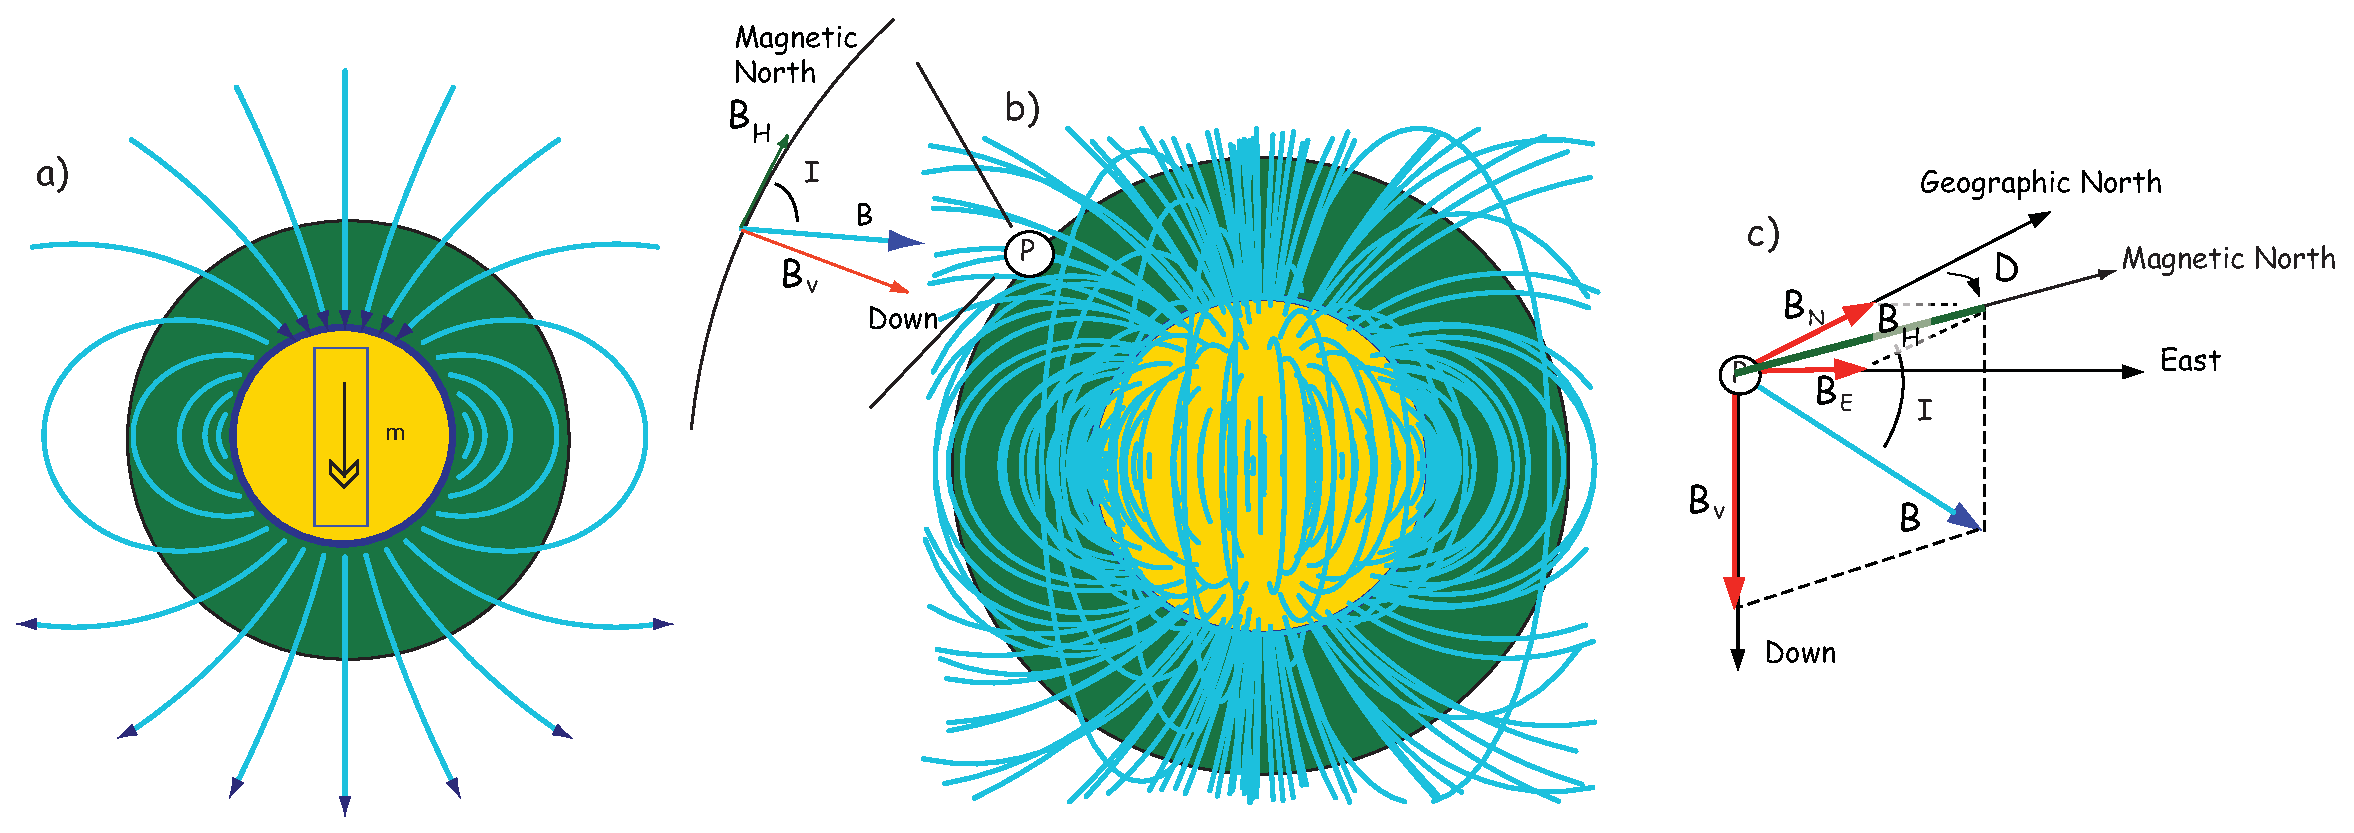
\includegraphics[width=14.5 cm]{EPSfiles/components.eps}
\caption{a) Lines of flux produced by  a geocentric axial dipole.  b) Lines of flux  of the geomagnetic field of 2005.   At point P the horizontal component of the  field $B_H$, is directed toward the magnetic north.  The vertical component $B_V$ is directed down and the field makes an angle $I$ with the horizontal, known as the
%\index{inclination}%
inclination.  c) Components of the geomagnetic field vector $\B$.  The angle between the horizontal component (directed toward magnetic north and geographic north is the 
declination $D$.) [Modified from Ben-Yosef et al., 2008b.] 
}
\label{fig:coord}
\end{figure}
\nocite{benyosef08b}

\index{magnetic!field!components}
Although dominantly dipolar, the  geomagnetic field is not perfectly modeled by a geocentric axial dipole, but is somewhat more complicated (see Figure~\ref{fig:coord}b).  At the point on the surface labeled `P', the geomagnetic field points nearly north and down at an angle of approximately 60$^{\circ}$.   
Vectors in three dimensions are described by three numbers and in many paleomagnetic applications, these are two angles ($D$ and $I$) and the  strength ($B$)  as shown in  Figure~\ref{fig:coord}b and c.  The angle from the horizontal plane  is  the
\index{inclination}%
 {\it inclination} $I$; it  is positive downward and ranges from +90$^{\circ}$ for straight down to -90$^{\circ}$ for straight up.   If the geomagnetic field were that of a perfect GAD field, the horizontal component of the magnetic field ($B_H$ in Figure~\ref{fig:coord}b)  would point directly toward geographic  north.  In most places on the Earth there is a deflection away from geographic north and  the angle between geographic and magnetic north is the
\index{magnetic!declination}%
 {\it declination}, $D$ (see Figure~\ref{fig:coord}c).  $D$ is measured positive clockwise from  North  and  ranges from $0 \rightarrow 360^\circ$.   [Westward declinations can also be expressed as negative numbers, i.e., 350$^{\circ}$ = -10$^{\circ}$.]   The vertical component ($B_V$  in Figure~\ref{fig:coord}b,c) of the geomagnetic field at P, is given by 

\begin{equation}
B_V = B \sin I,
\label{eq:Bv}
\end{equation}   
\noindent and the horizontal component $B_H$  (Figure~\ref{fig:coord}c) by
\begin{equation}
B_H = B \cos I.
\label{eq:Bh}
\end{equation}  

\noindent    $B_H$
can  be  further resolved into north and east components ($B_N$ and $B_E$ in Figure~\ref{fig:coord}c) by


\begin{equation}
 B_N=B \cos I \cos D \hskip 1em \hbox{ and } \hskip 1em B_E=B \cos I \sin D .
\label{eq:BnBe}
\end{equation}





Depending on
the particular problem, some 
\index{coordinate systems}%
coordinate systems are more suitable to
use because they have the symmetry of the problem built into them.    We have just defined a coordinate system using two angles and a length ($B,D,I$) and the equivalent 
\index{coordinate systems! Cartesian}%
Cartesian coordinates of  ($B_N, B_E, B_V$). We
will need to convert among them at will.  There are many names for the Cartesian coordinates. In addition to north, east and down, they  could also be $x,y,z$ or even
 $x_1, x_2$ and $x_3$. 
The convention used in
this book is that axes are denoted $\X_1, \X_2, \X_3$, while the components
along the axes are frequently designated $x_1, x_2, x_3$.  In the geographic frame of reference,
positive $\X_1$ is to the north, $\X_2$ is east and $\X_3$ is vertically 
down in keeping with the right-hand rule.    To convert from  Cartesian coordinates to angular coordinates ($B,D,I$):

\beq
B = \sqrt{x_1^2 +x_2^2 + x_3^2}, \hskip 1em
D=\tan^{-1} {x_2\over{x_1}}, \hbox{ and }
I=\sin^{-1} {x_3\over B}.
\label{eq:DI}
\eeq

\noindent Be careful of the sign ambiguity of the tangent function. You may well end up
in the wrong quadrant and have to add 180$^{\circ}$; this will happen if both $x_1$ and $x_2$ are negative.  In most computer languages, there is a function {\bf atan2} which takes care of this, but most hand calculators will not.     Remember that most computer languages expect angles to be given in radians, not degrees, so multiply degrees by $\pi/180$ to convert to radians.  Note also that in place of $\B$ for magnetic induction with units of tesla as  a measure of vector length, (see Chapter 1), we could also use $\H$,  $\M$ ( both Am$^{-1}$) or $\m$ (Am$^2)$ for magnetic  field, magnetization or magnetic moment respectively.  




\section {Reference magnetic field}
\label{sect:igrf}

We can measure 
\index{magnetic!declination}
\index{magnetic!inclination}
\index{magnetic!intensity}
declination, inclination and intensity at different places around the globe, but not everywhere all the time.  Yet it is often handy to be able to predict what these components are.  For example, it is extremely useful to know what the deviation is between true North and declination in order to find our way with maps and compasses.  
In principle,   magnetic field vectors can  be derived from the 
\index{magnetic!potential}
 magnetic potential $\psi_m$ as we showed in Chapter 1. For an axial dipolar field, there is but one scalar coefficient (the magnetic moment $\m$ of a dipole source).  For the geomagnetic field,  there are many more coefficients,  including not just an axial dipole aligned with the spin axis, but two orthogonal equatorial dipoles and a whole host of more complicated sources such as quadrupoles, octupoles and so on.  A list of coefficients associated with these sources   allows us to calculate the magnetic field vector anywhere outside of the source region.   In this section, we outline how this might be done.  


As we learned in Chapter 1, the magnetic field at the Earth's surface
can be calculated  from the gradient of a  scalar potential field ($\H=-\nabla \psi_m$), and this scalar potential field
satisfies
\index{Laplace's equation}
 Laplace's Equation:

\begin{equation}
 \nabla^2 \psi_m = 0.
 \label{eq:laplace}
\end{equation}


\noindent For the geomagnetic field (ignoring external sources of the magnetic field which are in any case small and transient), the potential equation can be written  as:
%\beq
%  \psi_m (r,\theta,\phi)={a \over {\mu_o}} \sum_{l=1}^\infty \sum_{m=0}^l P_l^m (\cos \theta)
%\Biggl[g_l^m \left({a \over
%r}\right)^{l+1} \cos m\phi  + h_l^m \left({a \over
%r}\right)^{l+1}\sin m\phi \Biggr],
%\label{eq:V}
% \end{equation}
\beq
  \psi_m (r,\theta,\phi)={a\over{ \mu_o} } \sum_{l=1}^\infty  \sum_{m=0}^l \left( {a \over
r}\right)^{l+1} P_l^m (\cos \theta)
\left(g_l^m  \cos m\phi  + h_l^m \sin m\phi\right),
\label{eq:V}
 \end{equation}


\noindent where $a$ is the radius of the
Earth ($6.371 \cross 10^6$ m).    In addition to the radial distance $r$ and the angle away from the pole $\theta$, there is $\phi$, the angle around the equator from some reference, say, the Greenwich meridian.  Here, $\theta$ is the co-latitude and $\phi$ is the longitude. 
The  $g_l^m$s and $h_l^m$s are the
\index{Gauss!coefficients}%
 {\it gauss coefficients} (degree $l$ and order $m$)   for hypothetical sources at radii less than $a$
calculated for a particular year. These are normally given in units of nT.  The
$P_l^m$s are  wiggly functions called partially normalized 
Schmidt polynomials of the argument $\cos \theta$. These are closely related to the associated
\index{Legendre polynomials}%
 Legendre polynomials.  [When $m=0$ the 
 \index{Schmidt polynomials}%
Schmidt and Legendre polynomials are identical.]  The first few of $P_l^m$s are: 
$$
P_1^0=\cos \theta, P_2^0 = {1\over 2}(3\cos^2\theta -1), \hbox{ and }	
P_3^0 = {1\over 2}\cos \theta(5\cos^3\theta -3\cos \theta ),
$$
\noindent and are shown in Figure~\ref{fig:schmidt}. 

\begin{figure}[htb]
%\epsfxsize 11cm
%\centering \epsffile{EPSfiles/schmidt.eps}
\centering  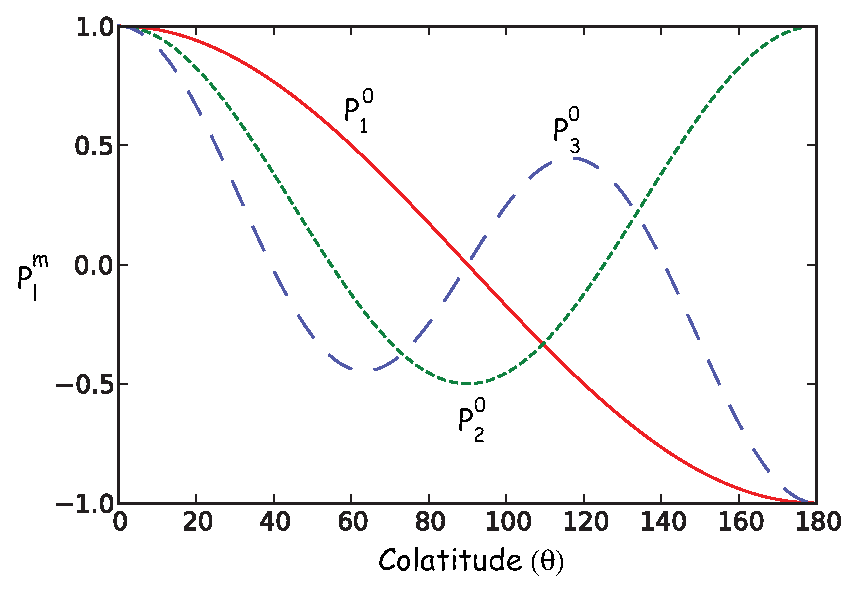
\includegraphics[width=11 cm]{EPSfiles/schmidt.eps}
\caption{Schmidt polynomials.}
\label{fig:schmidt}
\end{figure}


\index{spherical!harmonics}
To get an idea of how the  gauss coefficients in the potential relate to the associated magnetic fields, we show three examples 
 in  Figure~\ref{fig:harmonics}.  We plot the inclinations of the vector fields   that would be produced by the terms with $g_1^0, g_2^0$ and $g_3^0$ respectively.  
 \index{spherical!harmonics!dipole term}
 \index{spherical!harmonics!quadrupole term}
 \index{spherical!harmonics!octupole term}
 These are the axial ($m=0$)  dipole ($l=1$), quadrupole ($l=2$) and octupole ($l=3$) terms. 
The  associated potentials for each harmonic  are shown in the   insets.  
 
 \begin{figure}[htb]
%\epsfxsize 14.5cm
%\centering \epsffile{EPSfiles/harmonics.eps}
\centering  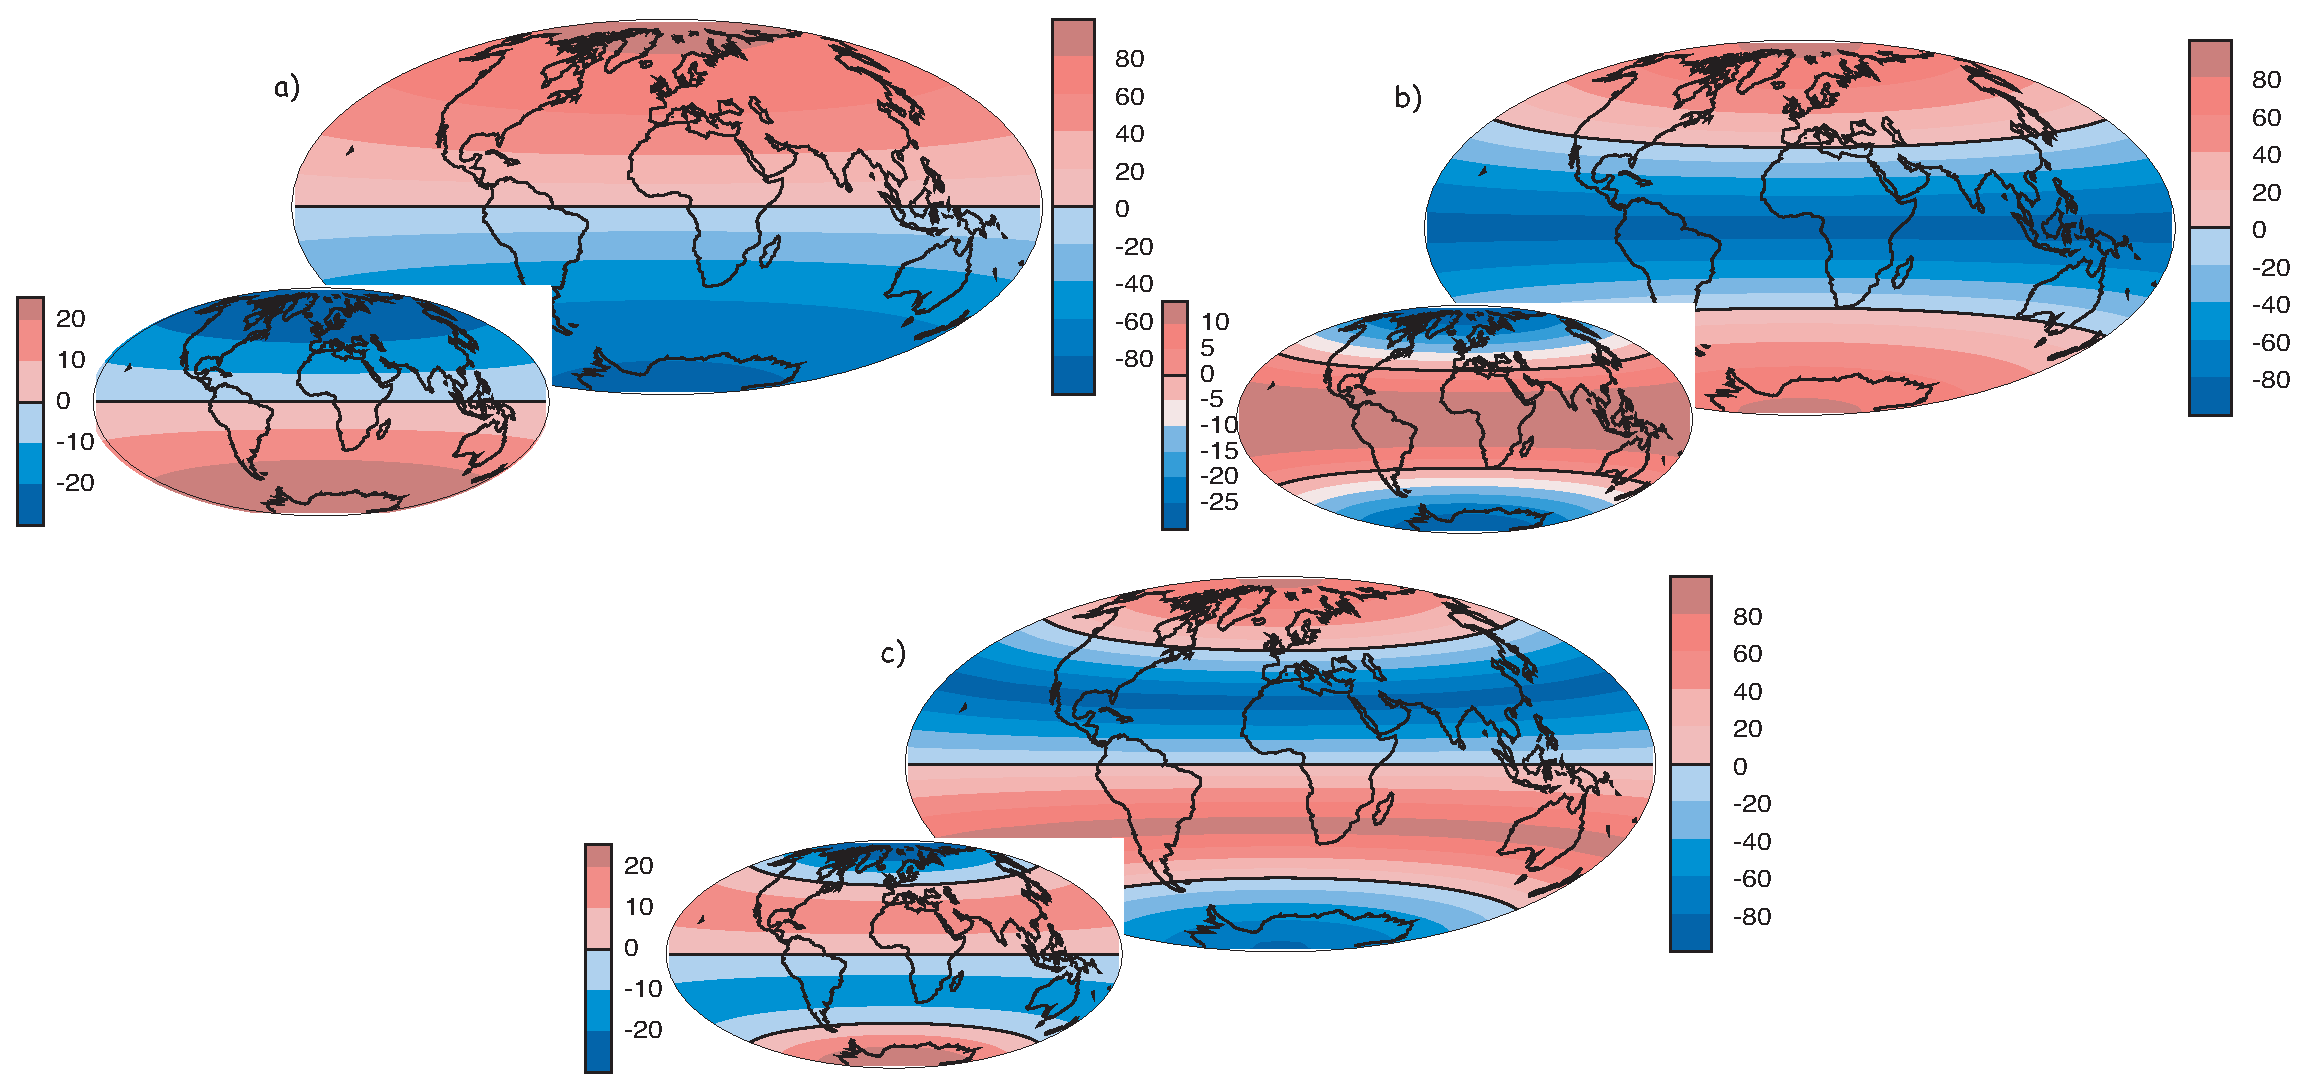
\includegraphics[width=14.5 cm]{EPSfiles/harmonics.eps}
\caption{Examples of potential fields (insets)  and maps of  the associated patterns for global inclinations.  Each coefficient is set to 30 $\mu$T.   a) Dipole ($g_1^0=30 \mu$T), b) Quadrupole ($g_2^0=30 \mu$T), c) Octupole ($g_3^0=30 \mu$T).    }
\label{fig:harmonics}
\end{figure}


  In general, terms for which the difference between the subscript ($l$) and the superscript ($m$) is odd (e.g., the axial dipole $g_1^0$ and octupole $g_3^0$)  produce magnetic fields that are antisymmetric about the equator, while those for which the difference is even (e.g., the axial quadrupole $g_2^0$) have symmetric fields.  In Figure~\ref{fig:harmonics}a we show the inclinations produced by a purely dipolar field of the same sign as the present day field.  The inclinations are all positive (down) in the northern hemisphere and negative (up) in the southern hemisphere.  In contrast, inclinations produced by a purely quadrupolar field (Figure~\ref{fig:harmonics}b) are down at the poles and up at the equator.    The map of inclinations produced by a purely axial octupolar field (Figure~\ref{fig:harmonics}c) are again asymmetric about the equator  with  vertical directions of opposite signs at the poles separated by bands with the opposite sign at mid-latitudes.    

As noted before, there is not one, but three dipole terms in Equation~\ref{eq:V},   the axial term ($g_1^0$) and two equatorial terms ($g_1^1$ and $h_1^1$).  
Therefore, the total dipole contribution is the vector sum of these three or $\sqrt{{g_1^0}^2+{g_1^1}^2+{h_1^1}^2}$.   The total quadrupole contribution ($l=2$) combines five coefficients and the total octupole ($l=3$)  contribution combines seven coefficients.  
 




So how do we get this marvelous list of gauss coefficients?  If you want to know the details, please refer Langel (1987). \nocite{langel87}  We will just give a brief introduction here.  
Recalling Chapter 1, once the scalar potential $\psi_m$ is known, 
the components of the magnetic field can
be calculated from it.  We solved this for the radial and tangential field components ($H_r$ and $H_{\theta}$)  in Chapter 1.   We will now change 
\index{coordinate systems}%
coordinate  and unit systems  and introduce a third dimension (because the field is not  perfectly dipolar).   The north, east, and vertically down components are related to the potential  $\psi_m$ by:

\begin{equation} 
B_N=-{\mu_o\over r}  {{\partial \psi_m} \over { \partial  \theta}},
 B_E=-{\mu_o\over {r \sin \theta }} {{\partial \psi_m} \over {\partial \phi}},
 B_V=-{\mu_o{\partial \psi_m} \over{ \partial r}}.
\label{eq:BnBeBv}
 \end{equation}


\noindent where $r$, $\theta$, $\phi$ are radius, co-latitude (degrees
away from the North pole) and longitude,
respectively. Here, $B_V$ is positive down, $B_E$ is positive east, and  $B_N$ is positive to the north, the opposite of
$H_r$ and $H_{\theta}$ as defined in Chapter 1. Note that
Equation~\ref{eq:BnBeBv} is in units of induction, not Am$^{-1}$ if the units for the gauss coefficients are in  nT, as is the current practice.     

Going backwards, 
the gauss coefficients  are determined by fitting 
Equations~\ref{eq:BnBeBv}
 and \ref{eq:V} to observations
of the magnetic field made by magnetic observatories or satellite for a particular time.
The {\it International (or Definitive) Geomagnetic Reference
Field}  or  I(D)GRF,  for a given time interval is an agreed upon set of values for a
number of gauss coefficients and their time derivatives.  
\index{Field models!IGRF}%
\index{Field models!IDGRF}%
IGRF (or DGRF) models and programs
for calculating various components of the magnetic field
are available on the internet from the 
National Geophysical Data Center; the address is \url{http://www.ngdc.noaa.gov}.  there is also a program {\bf igrf.py} included in the {\bf PmagPy} package (see \href{http://earthref.org/PmagPy/cookbook/#igrf.py}{igrf.py documentation}).   

In practice, the   gauss
coefficients for a particular reference field are estimated by least-squares fitting of  observations of the geomagnetic field.  You need a minimum of  48
observations to estimate the coefficients to $l=6$.  Nowadays, we have satellites which give us  thousands of measurements and the list of generation 10 of the IGRF for 2005 goes to $l=13$.  


\begin{table}[h!tb]
\begin{center}
\caption {IGRF,  12$^{th}$ generation (2015) to $l=6$. (Thebault et al., 2015)}
\label{tab:igrf15}
\begin{tabular}{r r r r|rrrr}
\hline
$l$&$m$&$g $( nT) &$h$ (nT) & $l$&$m$&$g $( nT) &$h$ (nT) \\
\hline
1 & 0 & -29442.0 & 0 & 5 & 0 & -232.6 & 0\\
1 & 1 & -1501.0 & 4797.1 & 5 & 1 & 360.1 & 47.3\\
2 & 0 & -2445.1 & 0 & 5 & 2 & 192.4 & 197.0\\
2 & 1 & 3012.9 & -2845.6 & 5 & 3 & -140.9 & -119.3\\
2 & 2 & 1676.7 & -641.9 & 5 & 4 & -157.5 & 16.0\\
3 & 0 & 1350.7 & 0 & 5 & 5 & 4.1 & 100.2\\
3 & 1 & -2352.3 & -115.3 & 6 & 0 & 70.0 & 0\\
3 & 2 & 1225.6 & 244.9 & 6 & 1 & 67.7 & -20.8\\
3 & 3 & 582.0 & -538.4 & 6 & 2 & 72.7 & 33.2\\ 
4 & 0 & 907.6 & 0 & 6 & 3 & -129.9 & 58.9\\
4 & 1 & 813.7 & 283.3 & 6 & 4 & -28.9 & -66.7\\
4 & 2 & 120.4 & -188.7 & 6 & 5 & 13.2 & 7.3\\
4 & 3 & -334.9 & 180.9 & 6 & 6 & -70.9 & 62.6\\ 
4 & 4 & 70.4 & -329.5 \\
 \hline
\end{tabular}
\end{center}
\end{table}
  \nocite{thebault15}


In order to get a feel for the importance of the various gauss coefficients, take a look at Table~\ref{tab:igrf15}, which has the Schmidt quasi-normalized gauss coefficients for the first six degrees from the IGRF for 2005.   
The power at each degree is the average squared field per spherical harmonic degree over the Earth's surface and is calculated by  $R_l=\sum_m (l+1)[(g_l^m)^2 + (h_l^m)^2]$
\index{Lowes, F.J.} \nocite{lowes74} 
(Lowes, 1974). 
The  so-called 
\index{Lowes spectrum}
{\it Lowes spectrum} is shown in 
Figure~\ref{fig:power}.  It is clear that the lowest order terms (degree one) totally
dominate,   constituting some 90\% of the field.    This is why the geomagnetic field is often assumed to be equivalent to a magnetic field created by a simple dipole at the center of the Earth.   



\begin{figure}[htb]
%\epsfxsize 11cm
%\centering \epsffile{EPSfiles/power.eps}
\centering  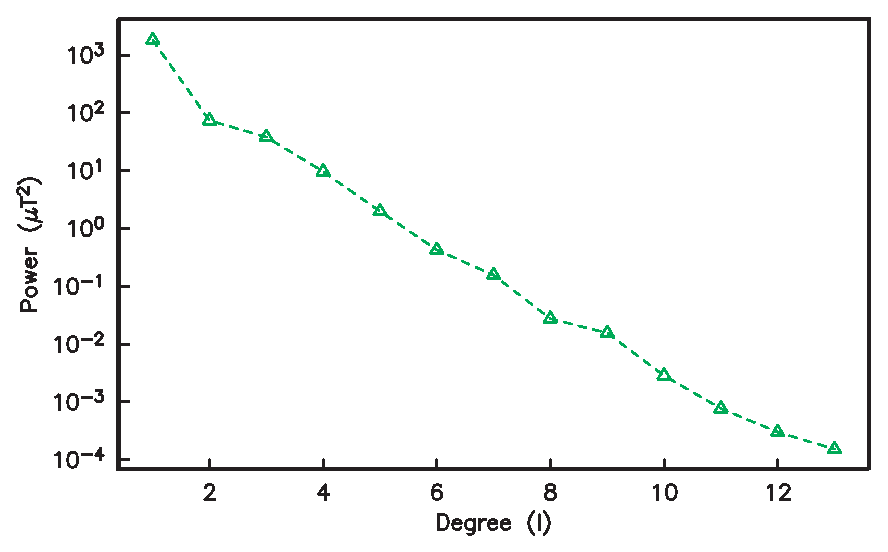
\includegraphics[width=11 cm]{EPSfiles/power.eps}
\caption{ Power at the Earth's surface of the geomagnetic field versus degree for the 2005 IGRF  (Table 2.1). }
\label{fig:power}
\end{figure}



\begin{figure}[htb]
 %\epsfxsize  14cm
%\centering \epsffile {EPSfiles/B.eps}
\centering  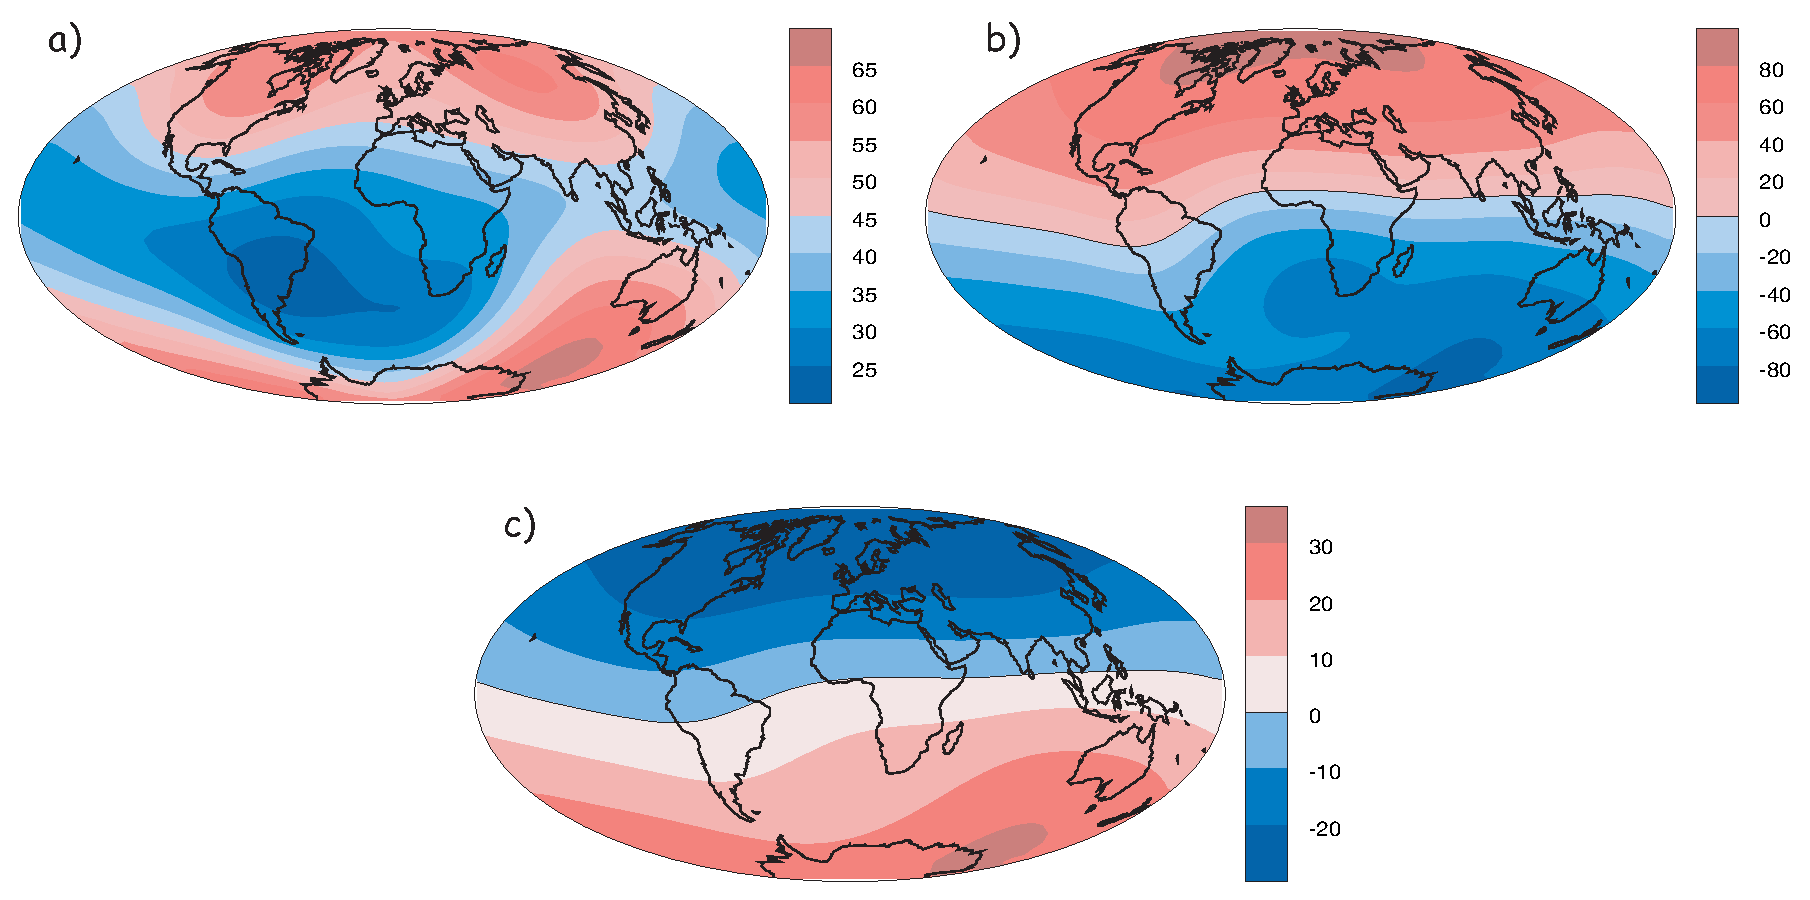
\includegraphics[width=14 cm]{EPSfiles/B.eps}
\caption {Maps of geomagnetic field of the IGRF for 2005.
a) Intensity (units of $\mu$T), b) inclination, c) potential (units of nT).}
\label{fig:B}
\end{figure}



\section{Geocentric axial dipole (GAD) and other poles}
\label{sect:gad}

The beauty of using the geomagnetic potential field is that the vector field can be evaluated anywhere outside the source region.      Using the 
values for a given reference field in   
  Equations~\ref{eq:V} and \ref{eq:BnBeBv}, we can   calculate
 values of $B, D$ and $I$ at any location on Earth.    Figure~\ref{fig:coord}b shows the lines of flux predicted from the 2005 IGRF from  the core-mantle boundary up.   We can see that the field becomes simpler and more dipolar as we move from the core mantle boundary to the surface.  Yet, there is still significant non-dipolar structure in the geomagnetic field even at the Earth's surface.  
 
   We can recast the vectors at the surface of the Earth into  maps of components as  shown in 
Figure~\ref{fig:B}a,b.   
We show the potential in Figure~\ref{fig:B}c for comparison with that of  a pure dipole (inset to Figure~\ref{fig:harmonics}a).      These maps illustrate the fact that
the field is a complicated function of position on the surface of the Earth.  
The intensity values in Figure~\ref{fig:B}a are, in
general,  highest near the poles ($\sim$ 60 $\mu$T) and lowest near the equator
($\sim$ 30 $\mu$T), but the contours are not straight lines parallel to latitude
as they would be for a field generated strictly by a 
\index{Field models!geocentric axial dipole}
geocentric axial dipole (GAD) (e.g, Figure~\ref{fig:coord}a).  
 Similarly, a GAD would produce lines of 
inclination that vary in a regular way from -90$^{\circ}$ to +90$^{\circ}$
at the poles, with 0$^{\circ}$ at the equator;  the contours
would parallel the lines of latitude.  Although the general trend in inclination
shown in Figure~\ref{fig:B}b is similar to the GAD model, the field lines are more complicated, which again suggests that the field is not perfectly
described by a geocentric bar magnet. 





\begin{figure}[htb]
%\epsfxsize 9cm
%\centering \epsffile{EPSfiles/poles.eps}
\centering  \includegraphics[width=9 cm]{EPSfiles/poles.eps}
\caption{Different poles.  
The square is the magnetic North Pole, where the magnetic field is straight
down $(I = +90^{\circ})$ (82.7$^{\circ}$N, 114.4$^{\circ}$W for  the IGRF 2005); the circle is the geomagnetic North Pole, where the axis of the
best fitting dipole pierces the surface (9.7$^{\circ}$N, 71.8$^{\circ}$W for the  IGRF 2005). 
 The star is the geographic North Pole.  [Figure made using Google Earth with seafloor topography of  D. Sandwell supplied to Google Earth by  D. Staudigel.]}
\label{fig:poles}
\end{figure}




Perhaps the most important result of
\index{spherical!harmonics}%
spherical harmonic analysis for our purposes is that the field at the Earth's surface is dominated
by the degree one terms ($l=1$) and the external contributions are very
small.
  The first order terms can be thought of as geocentric dipoles that are aligned
with three different axes: the spin axis ($g_1^0$) and two equatorial axes 
that intersect the equator at the Greenwich meridian 
($h_1^0$) and at 90$^{\circ}$ East ($h_1^1$).               
\index{pole!geomagnetic}%
\index{geomagnetic!pole}%
The vector sum of these geocentric dipoles  is a dipole that is currently
 inclined by about 10$^{\circ}$ to the spin axis.  The
axis of this {\it best-fitting dipole} pierces the surface of the Earth at the circle in
Figure~\ref{fig:poles}.  This point and its antipode are called
 {\it geomagnetic poles}.  Points at which the field
is vertical ($I = \pm 90^{\circ}$ shown by a square in Figure~\ref{fig:poles}) are called  
{\it magnetic poles}, or sometimes 
\index{pole!magnetic}%
\index{magnetic!pole}%
\index{pole!dip}%
\index{dip pole}%
{\it dip poles}.  These poles are distinguishable from the {\it geographic poles},
  where the spin axis of the Earth intersects its surface.
The northern geographic pole is shown by a star in Figure~\ref{fig:poles}.

\index{pole!geographic}%
\index{geographic pole}%
It turns out that when averaged over sufficient time, the geomagnetic field  actually does seem  to be  approximately  a GAD field, perhaps with a pinch of $g_2^0$ thrown in
\index{Merrill, R.T.} \nocite{merrill96}
 (see e.g., Merrill et al., 1996). 
The GAD model of the field will serve as a useful crutch 
throughout our discussions of
paleomagnetic data and applications. 
Averaging ancient magnetic poles over enough time to average out secular variation (thought to be  10$^4$ or 10$^5$ years)  gives what is known
as a 
\index{pole!paleomagnetic}%
{\it paleomagnetic pole}; this  is usually assumed to be co-axial with the Earth's geographic pole (the spin axis).  


Because the geomagnetic field is axially dipolar 
to a  first approximation, we can write:

\beq \psi_m= {a\over{\mu_o} }g_1^0 \left({a \over r} \right)^2 P_1^0 ( \cos \theta ) = {a\over{\mu_o} } g_1^0
\left( {a \over r} \right)^2 \cos \theta.
\label{eq:Vmdip}
\eeq

 Note that $g_1^0$ is given in nT in Table~\ref{tab:igrf15}.    Thus, from Equation~\ref{eq:Vmdip}, 

\begin{equation} 
{B_N}=\mu_o H_N= {g_1^0 a^3 \sin \theta \over r^3}, \hskip 1em B_E=0, \hskip 1em \hbox{and} \hskip 1em
 B_V=\mu_o H_V=  {2 g_1^0 a^3 \cos \theta
\over r^3}.
\label{eq:Bnevdip}
 \end{equation}

\noindent Given some latitude $\lambda$
 on the surface of the Earth 
 in  Figure~\ref{fig:coord}a
and using the equations for $B_V$ and $B_N$, we find that:

\begin{equation} \tan  I = {B_V \over B_N} = 2 \cot  
\theta = 2 \tan \lambda.
\label{eq:dipform}
 \end{equation} 

\index{dipole!formula}%
\index{dipole!equation}%
\noindent This equation is sometimes called the {\it dipole formula}  and
shows that the inclination of the magnetic field
 is directly related to the co-latitude  ($\theta$) for a
 field produced by a geocentric axial dipole (or $g_1^0$). The dipole formula allows us to
calculate the latitude of the measuring position from the inclination of the
(GAD) magnetic field, a result that is fundamental in plate tectonic reconstructions. 
The intensity of a dipolar magnetic 
field is also related to (co)latitude because:

\beq 
 B = (B_V^2 + B_N^2 )^\half
= {g_1^0 a^3 \over r^3} ( \sin^2 \theta + 4 \cos^2 \theta)^{1\over 2}
 = {g_1^0 a^3 \over r^3} ( 1 + 3 \cos^2 \theta)^\half.
\label{eq:Bvdip}
\eeq

\noindent The dipole field intensity has changed by more than an order of magnitude 
in the past and the dipole relationship of intensity to latitude
 turns out to be not useful for tectonic reconstructions.  

 

\section{Plotting magnetic directional data}
\label{sect:eqarea}


Magnetic field and magnetization directions 
can be visualized as unit vectors anchored at the center of
a unit sphere. Such a unit sphere is difficult to represent on a 2-D page.
There are several popular projections, including the
Lambert equal area projection which we will be making extensive use
of  in later chapters.  The principles of
construction of the equal area projection 
are covered in the Appendix~\ref{app:eqarea}.

In general, regions of equal area on the sphere project as equal
area regions on this projection, as the name implies.  
Plotting directional data in this way  enables rapid
assessment of data scatter.  A drawback
of this projection is that circles 
on the surface of a sphere project as ellipses.  Also, because we have
projected a vector onto a unit sphere, we have lost
information concerning the magnitude of the vector.
Finally, lower and upper hemisphere projections must be distinguished
with different symbols.  The paleomagnetic  convention is:
lower hemisphere projections (downward directions)  use solid
symbols, while upper hemisphere projections
are open. 

\begin{figure}[htb]
%\epsfxsize 11cm
%\centering \epsffile{EPSfiles/igrf.eps}
\centering  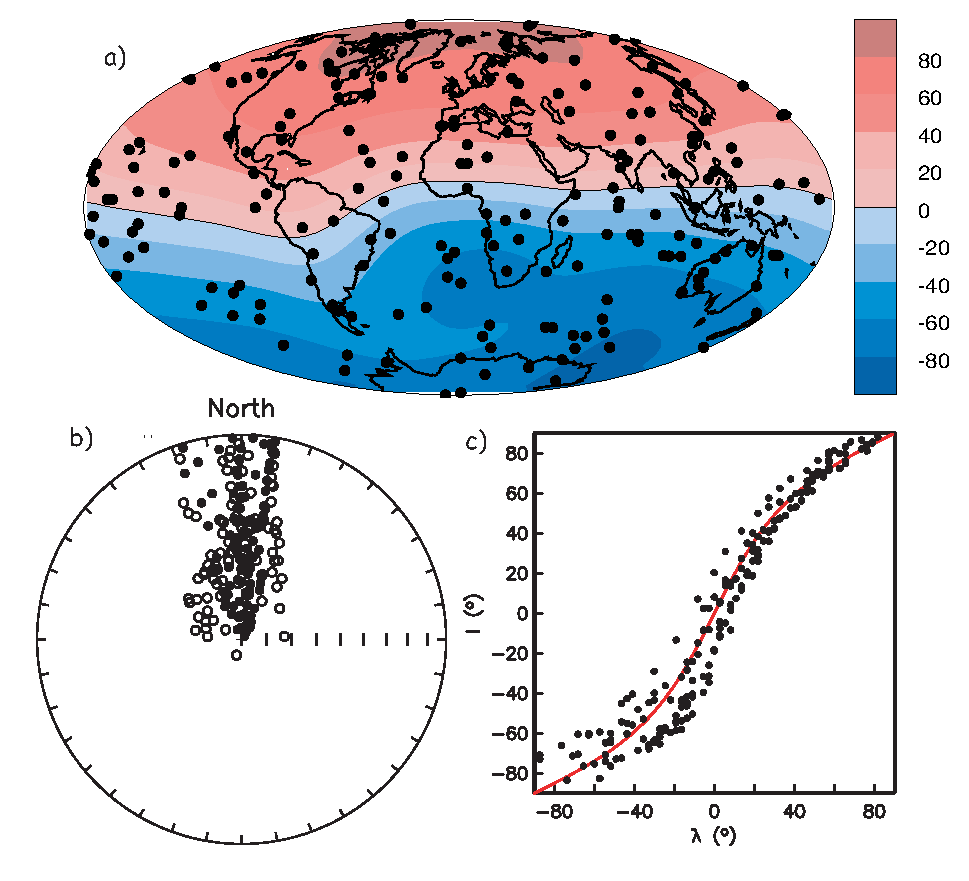
\includegraphics[width=11 cm]{EPSfiles/igrf.eps}
\caption{
a) Hammer projection of 200 randomly selected locations around the globe.
b) Equal area projection of directions of Earth's magnetic field as given 
by the
IGRF evaluated for the year 2005 at locations shown in a). Open (closed)
symbols indicate upper (lower) hemisphere. c) Inclinations
(I) plotted as a function of site latitude ($\lambda$). 
The solid line is the inclination
expected from the dipole formula (see text). Negative latitudes are
south and negative inclinations are up. [Figure redrawn from Tauxe, 1998.]}
\label{fig:igrf}
\end{figure}
\nocite{tauxe98}


The dipole formula allows us to convert a given measurement of $I$ to an equivalent
\index{magnetic!colatitude}
 {\it magnetic
co-latitude} $\theta_m$:

\beq
\cot \theta_m = \half \tan I.
\label{eq:mcolat}
\eeq

If the field were a simple GAD field,  $\theta_m$ would be a reasonable estimate of
$\theta$, but non-GAD terms can invalidate this assumption.   To get a feel for the effect of these non-GAD terms, we
consider first what would happen if we took random measurements of the
Earth's present field (see Figure \ref{fig:igrf}).  We evaluated the 
directions of the magnetic field  using the IGRF for 
2005 at   200 positions on the globe (shown in 
Figure~\ref{fig:igrf}a).  These directions are plotted in
Figure~\ref{fig:igrf}b using the paleomagnetic convention 
of open symbols pointing up and closed symbols pointing down.  
In
Figure~\ref{fig:igrf}c, we plot the inclinations as a function of latitude.
As expected from a predominantly dipolar field, 
inclinations cluster around the values for a geocentric axial
dipolar field but there is considerable scatter and interestingly the scatter is larger in the southern hemisphere than in the northern one.   This is related to the low intensities beneath South America and the Atlantic region seen in Figure~\ref{fig:B}a. 

\subsection{$D', I' $ transformation}  

Often we wish to compare directions from distant parts of the globe.  There is an inherent difficulty in doing so because of the large variability in inclination with latitude.  
In such cases it is appropriate to  consider the data relative to the expected direction (from GAD) at each sampling 
site.  For this purpose, it is useful to use a transformation   
whereby each direction is rotated such that the  direction expected from a
geocentric axial dipole field (GAD) at the sampling site is the center of the equal 
area projection.  This is accomplished as follows:

Each direction is converted to Cartesian coordinates ($x_{i}$) by:

\begin{equation}
x_{1}= \cos D \cos I; \hskip 1em
x_{2}= \sin D \cos I; \hskip 1em x_{3}= \sin I.
\label{eq:dir2cart}
\end{equation}

\noindent
These are rotated to the new coordinate system ($x'_{i}$, see Appendix~\ref{app:tensors}) by:
$$
x'_{1}= (x_{1}^{2}+x_{3}^{2})^{1/2} \sin (I_{d} - \alpha); \hskip 1em
x'_{2}=x_{2}; \hskip 1em
x'_{3}=(x_{1}^{2}+x_{3}^{2})^{1/2} \cos (I_{d} - \alpha),
$$

\noindent
where $I_{d}$ = the inclination expected from a GAD field ($\tan 
I_{d}=2\tan \lambda$),  $\lambda$ is the site latitude, and $\alpha $ 
is the inclination of the paleofield vector projected onto the N-S 
plane ($\alpha = \tan^{-1} (x_{3}/x_{1})$).   The $x'_{i}$ are then 
converted to $D',I'$ by Equation~\ref{eq:DI}. 

In Figure~\ref{fig:didip}a we show the geomagnetic field vectors evaluated at random longitudes along a latitude band of 45$^{\circ}$N.  The vectors are shown in their Cartesian coordinates of North, East and Down.  In Figure~\ref{fig:didip}b we show what happens when we rotate the coordinate system to peer down the direction expected from an axial dipolar field at 45$^{\circ}$N (which has an inclination of 63$^{\circ}$).    The vectors circle about the expected direction.    Finally,   
we see what happens to the directions shown in 
Figure~\ref{fig:igrf}b after the $D',I'$ transformation in Figure~\ref{fig:didip}.   These are unit vectors projected along the expected direction for each observation  in Figure~\ref{fig:igrf}a.   Comparing the equal area projection of the directions themselves (Figure~\ref{fig:igrf}b) to the transformed directions (Figure~\ref{fig:didip}c), we see that the latitudal dependence of the inclinations has been removed. 

\begin{figure}[htb]
%\epsfxsize 14cm
%\centering \epsffile{EPSfiles/igrf.dip.eps}
\centering  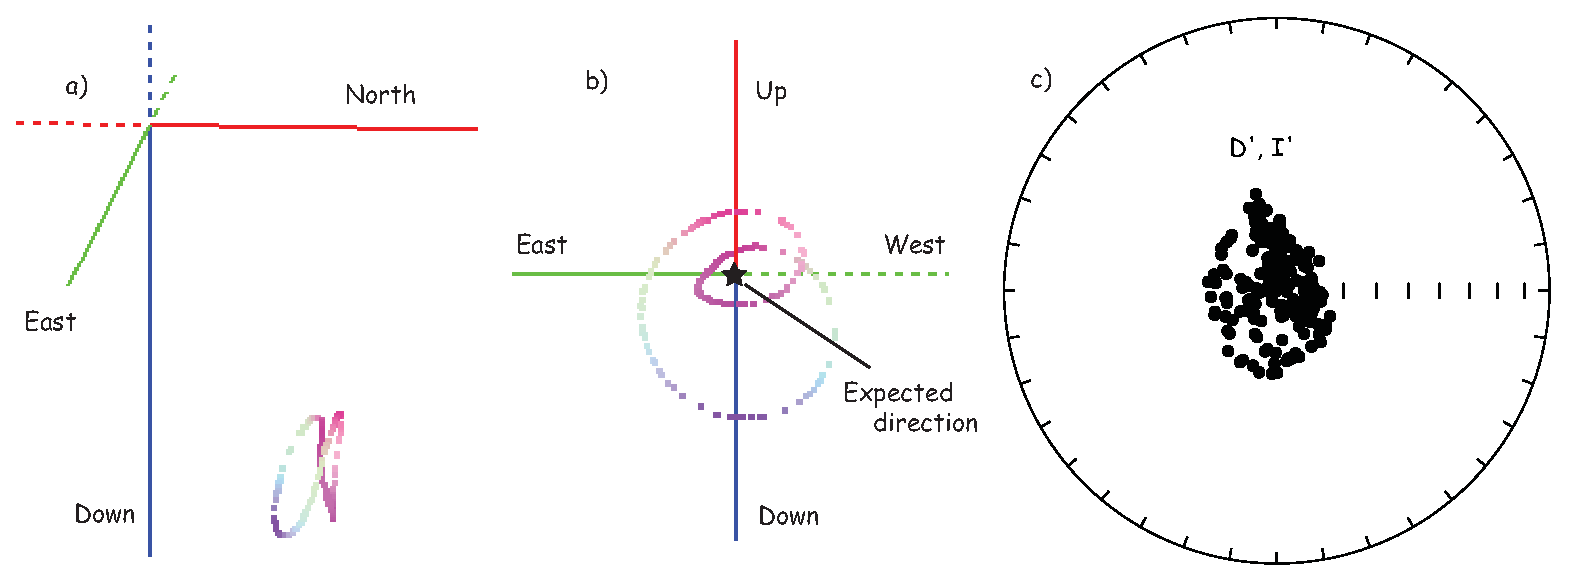
\includegraphics[width=14 cm]{EPSfiles/igrf_dip.eps}
\caption{a) Vectors evaluated around the globe at 45$^{\circ}$N.  Red/green/blue colors reflect the North, East and Down components respectively.  b) The unit vectors  (assuming unit length) from a).  c) Directions from Figure 2.7b transformed using the $D', I'$ transformation.}
\label{fig:didip}
\end{figure}


\begin{figure}[!htb]
%\epsfxsize 13cm
%\centering \epsffile{EPSfiles/mkvgp.eps }
\centering  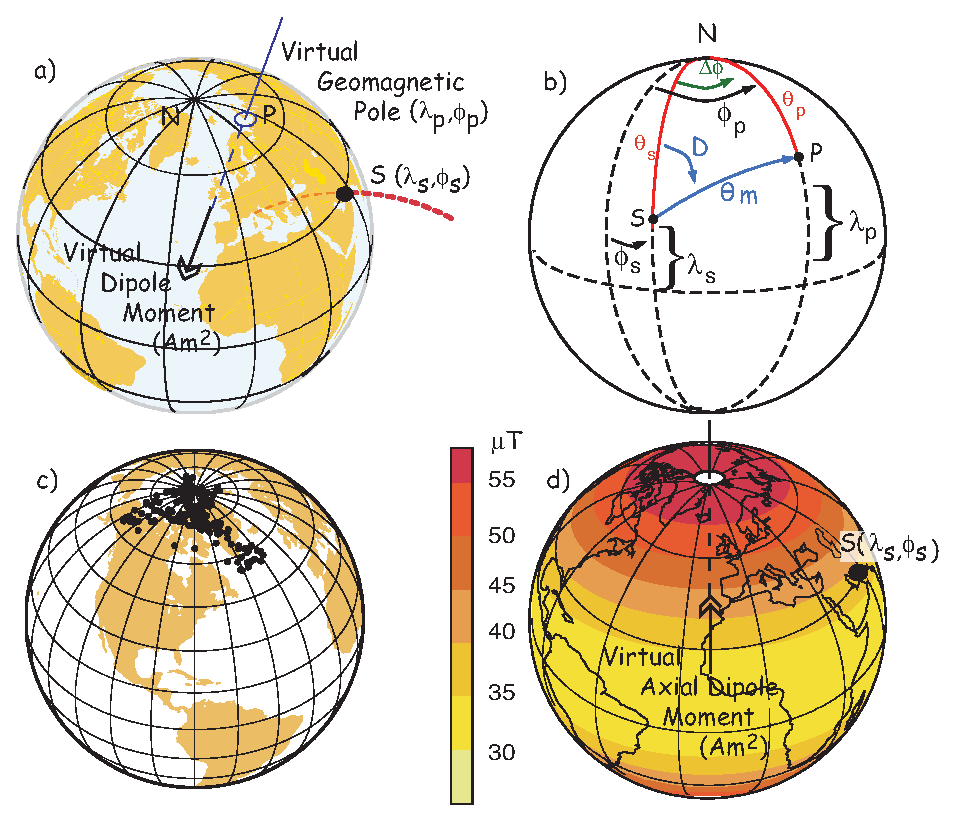
\includegraphics[width=13 cm]{EPSfiles/mkvgp.eps}
\caption {Transformation of a vector measured at S into a virtual
geomagnetic pole position (VGP) and virtual dipole moment (VDM),
using principles of spherical trigonometry and the dipole formula.  a) Red dashed line is the magnetic field line  observed at S (latitude of $\lambda_s$, longitude of $\phi_s$).  This field line is the  same as one produced by the VDM at the center of the Earth.  The point where the axis of the  VDM pierces the Earth's surface is the VGP.    b)  Observed declination (D) and inclination (converted to $\theta_m$ using the dipole formula (see text) defines angles $D$ and $\theta_m$.  $\theta_s$ is the colatitude of the observation site. N is the geographic North Pole (the spin axis of
the Earth). The position of the pole at P ($\theta_p,\phi_p$)  can be calculated with spherical trigonometry (see text).    c) VGP positions converted from directions shown in Figure 2.7b. d) The virtual axial dipole moment giving rise to the observed intensity at S.}
\label{fig:mkvgp}
\end{figure}

\customlink{Virtual_geomagnetic_poles}
\subsection{Virtual geomagnetic poles}
\label{sect:vgp}

 We are often interested in
whether the geomagnetic pole has changed, or whether a particular piece of crust
has rotated with respect to the geomagnetic pole.  Yet, what we
observe at a particular location is the local direction of the field
vector.  Thus, we need a way to transform an observed direction into the
equivalent geomagnetic pole. 

In order to remove the dependence of direction merely on position 
on the globe,  we imagine a geocentric dipole which would
give rise to the observed magnetic field direction
 at a given latitude ($\lambda$) and
longitude ($\phi$).  
\index{pole!virtual geomagnetic}%
\index{virtual!geomagnetic pole}%
The {\it virtual geomagnetic pole} (VGP) is the point
on the globe that corresponds to the geomagnetic pole of this imaginary dipole 
(Figure~\ref{fig:mkvgp}a).

Paleomagnetists use the following conventions:   $\phi$  is measured
positive eastward from the Greenwich meridian and
ranges from $0 \rightarrow 360^\circ$;  $\theta $  is measured  from
the North pole and goes from $0 \rightarrow 180^\circ$. Of course
$\theta $ relates
to latitude, $\lambda $ by $\theta = 90 - \lambda $.  $\theta_m$ is the
magnetic co-latitude and is given by Equation~\ref{eq:mcolat}. 
Be sure not to confuse latitudes and co-latitudes.
Also, be careful with 
\index{magnetic!declination}%
declination.  Declinations between 180$^\circ$
and 360$^{\circ}$ are equivalent to $D$ - 360 $^\circ$ which are
counter-clockwise with respect to North.  

The first step in the problem  of calculating a VGP is to determine the
\index{magnetic!colatitude}%
 magnetic co-latitude $\theta_m$ by Equation~\ref{eq:mcolat} which is defined in the dipole formula (Equation~\ref{eq:mcolat}).
The declination $D$ is the angle from the geographic
North Pole to the
great circle joining the observation site $S$ and the pole $P$, and $\Delta \phi$ is the difference
in longitudes between P and S, 
$\phi_p-\phi_s$.  Now we use some tricks from 
\index{spherical!trigonometry}%
spherical trigonometry as reviewed in Appendix~\ref{app:strig}.

 
We can  locate VGPs using the law of sines and the law of cosines. 
The 
\index{magnetic!declination}
declination $D$ is the angle from the geographic North Pole
to the
great circle joining $S$ and $P$ (see Figure~\ref{fig:mkvgp}) so:
 
\def\pih{{\pi \over 2}}
\beq \cos \theta_p = \cos \theta_s  \cos
\theta_m + \sin \theta_s \sin \theta_m \cos D, 
\label{eq:vgplat}
\eeq
 
\noindent which allows us to calculate the VGP co-latitude $\theta_p$. The
VGP latitude is given by:

$$
\lambda_p = 90 - \theta_p,
$$
\noindent so $90>\lambda_p>0$ in the northern hemisphere and
$0<\lambda_p<90$ in the southern hemisphere.
 
To determine $\phi_p$, we first calculate the angular difference between
the pole and site
longitude $\Delta \phi$.  
 
\beq {{\sin \Delta \phi}=  \sin \theta_m} \cdot { \sin D \over
\sin \theta_p } .
\label{eq:vgplong}
\eeq
 
\noindent  If $\cos \theta_m
\geq \cos \theta_s \cos \theta_p$, then $\phi_p = \phi_s+\Delta \phi$.
However, if $\cos \theta_m <
\cos \theta_s \cos \theta_p$ then
$\phi_p=\phi_s + 180 -\Delta \phi$.


Now we can convert the directions in
Figure~\ref{fig:igrf}b to 
\index{virtual!geomagnetic pole}%
VGPs (see Figure~\ref{fig:mkvgp}c).  The grouping 
of points is much tighter in Figure~\ref{fig:mkvgp}c than in the
equal area projection because the effect
of latitude variations in dipole fields has been removed.    
If a number of VGPs are averaged together, the average pole position is called a ``paleomagnetic pole''.  How to average poles and directions is the subject of Chapters 11 and 12.

The procedure for calculating a direction from a VGP is a similar procedure to that for calculating the VGP from the direction.    
\index{magnetic!colatitude}
Magnetic colatitude $\theta_m$ is calculated in exactly the same way as before and yields inclination from the dipole formula.   The declination can be calculated  by solving for $D$ in Equation~\ref{eq:vgplat} as:

$$
\cos D = { { \cos \theta_p - \cos \theta_s \cos \theta_m} \over { \sin \theta_s \sin \theta_m} }.
$$

\noindent
This equation works most of the time, but breaks down under some circumstances, for example, when the pole latitude is further to the south than the site latitude.   The following algorithm works in the more general case:



$$
D= - \tan^{-1} (  { { \cos D}\over { \sqrt{ C}  } }) + 90,
$$
\noindent where $C = |1- (\cos D)^2|$.     Also, if  $-90 < \Delta \phi <0$ or if $ \Delta \phi > 180$, then $D = 360 - D$.       
 
\index{virtual!dipole moment}%
\customlink{Virtual_dipole_moment}
\subsection {Virtual dipole moment}
\label{sect:vdm}

As pointed out earlier,  magnetic
intensity varies
 over the globe in a similar manner to inclination.   It is 
 often convenient to express
paleointensity values in terms of the equivalent geocentric dipole
moment
that would have produced the observed intensity at a specific  (paleo)latitude.
Such an equivalent  moment is called the {\it virtual dipole moment} (VDM) by
analogy to the VGP (see Figure~\ref{fig:mkvgp}a).  First, the magnetic
(paleo)co-latitude $\theta_m $ is calculated as before from the observed
inclination
and the dipole formula of Equation~\ref{eq:dipform}. Then, following the
derivation of Equation~\ref{eq:Bvdip}, we have

\beq \hbox {VDM} = {{4\pi r^3\over \mu_o} {{B}_{ancient}}
{{(1 + 3\cos^2 \theta_m)^{-{1\over 2}}}}}. 
\label{eq:vdm}
\eeq

\noindent Sometimes the site co-latitude as opposed to magnetic co-latitude
 is used in the above equation, giving a 
 \index{virtual!axial dipole moment}%
{\it virtual axial dipole moment} (VADM; see Figure~\ref{fig:mkvgp}d).

\vskip .5 in\noindent{SUPPLEMENTAL READINGS:} Merrill et al. (1996), Chapters 1 \& 2

\vskip 24pt
{\parindent 0pt \parskip 12pt 
\section{Problems}
 
For this and future problem sets, you will need the {\bf PmagPy}  package (see section in the Preface at the beginning of the book).  After you have installed this and properly set your path, you can import the functions from {\bf PmagPy} using these commands: 

\begin{verbatim}
import pmagpy.pmag as pmag
import pmagpy.ipmag as ipmag
import pmagpy.pmagplotlib as pmagplotlib
\end{verbatim}

Please consult the Jupyter notebook {\it PmagPy.ipynb} for more help  on using PmagPy functions within a notebook.  


{\bf Problem 1}


a) Write a python script in an Jupyter notebook
that converts
declination, inclination and intensity to North, East, and Down.   Read in the data in the file {\it Chapter\_2/ps2\_prob1\_data.txt}.  For this the {\bf loadtxt} function in the Numpy module will come in handy.   


b) Choose 10 random spots on the surface of the earth.  You can use the {\bf pmag.get\_unf} to generate a list for you.  Then 
use the {\bf ipmag.igrf} function   to  evaluate  the declination, inclination and intensity at each of these locations in January 2006.  As with all {\bf PmagPy} programs, and functions, you can find out what they do by printing out the doc string:
 you can find out what they do by getting the help message:

\begin{verbatim}
help(ipmag.igrf)
\end{verbatim}

\noindent  Calls like these generates  help messages which will help you to call the function properly.  



c) Take the vectors from the output of  Problem 1b and convert them to cartesian coordinates, using the  script you wrote in Problem 1a.  


{\bf Problem 2}

a) Plot the IGRF directions from Problem 1b  on an equal area projection by hand.    Use the equal area net provided in the Appendix.   Remember that the outer rim is  horizontal and the center of the diagram is vertical.  Azimuth goes around the rim with clockwise being positive.    Put a  thumbtack through the equal area (Schmidt) net and place a piece of tracing paper on the thumbtack. Mark the top of the stereonet with a tick mark on the tracing paper. 

To plot a direction,   rotate the tick mark of the tracing paper around  counter clockwise until the top of the paper is rotated by the declination of the direction. Then count tick marks toward the center from the outer rim (the horizontal) to the inclination angle, plot the point, and rotate back so that the tick is North again. Put all your points on the diagram.


b) Now use the {\bf ipmag} functions {\bf plot\_net } and {\bf plot\_di}.
 or write your own!  Both plots should look the same....


{\bf Problem 3}

You went to Wyoming (112$^{\circ}$ W and 36$^{\circ}$ N) to sample some Cretaceous rocks.  You measured a direction with a declination of 345$^{\circ}$ and an inclination of 47$^{\circ}$.  

a) What direction would you expect  from the present (GAD) field? 

b)  What is the virtual geomagnetic pole position corresponding to the direction you actually measured?  [Hint: Use the function {\bf pmag.dia\_vgp} in the {\bf PmagPy} module or for a challenge, write your own! ]



 


%
 %DONE 7/15/18
%\customlink{Induced_and_remanent_magnetism}



\chapter{Induced  and remanent magnetism}

{\parskip 0pt
\noindent BACKGROUND:   For a review of basic quantum mechanics and statistical mechanics, read relevant chapters from an introductory Chemistry text book.

\vskip 24pt


Scientists in the late 19th century thought that
it might be possible to exploit the magnetic record
retained in accidental records  to study the geomagnetic field in the past. 
Work in the mid 20th century provided  the theoretical and experimental basis
for presuming that such materials might retain a record of past geomagnetic
fields. There are
several books and articles that describe the subject in detail (see e.g.,
the supplemental readings).   We
present here a brief overview of theories on how rocks get and 
stay magnetized.  We will begin with magnetism at the atomic level caused by electronic orbits and spins giving rise to induced magnetizations.  Then we will see how electronic spins working in concert give rise to permanently magnetized substances (like magnetic minerals) making remanent magnetization possible.  

\section {Magnetism at the atomic level}
\label{sect:atomic}


We learned in Chapter 1  that magnetic fields are generated by electric currents.  Given that there are no wires leading into or out of permanent magnets, you may well  ask, ``Where are the currents?''  At the atomic level, the electric currents come from the motions of the electrons.  
From here quantum mechanics quickly gets esoteric, but  some rudimentary understanding is helpful.  In this chapter we will cover the bare minimum necessary to grasp the essentials of rock magnetism.   

In Chapter 1 we took the classical (pre-quantum mechanics) approach and suggested that the orbit of an electron about the nucleus could be considered a tiny electric current with a correspondingly tiny magnetic moment.  
\index{quantum!mechanics}
But quantum physics
tells us that this ``planetary'' view of the atom  cannot be true.  An electron zipping around a nucleus would generate radio waves,  losing energy and  eventually would  crash into the nucleus.  

\begin{figure}[htb]
%\epsfxsize 10cm
%\centering \epsffile{EPSfiles/1s.eps}
\centering  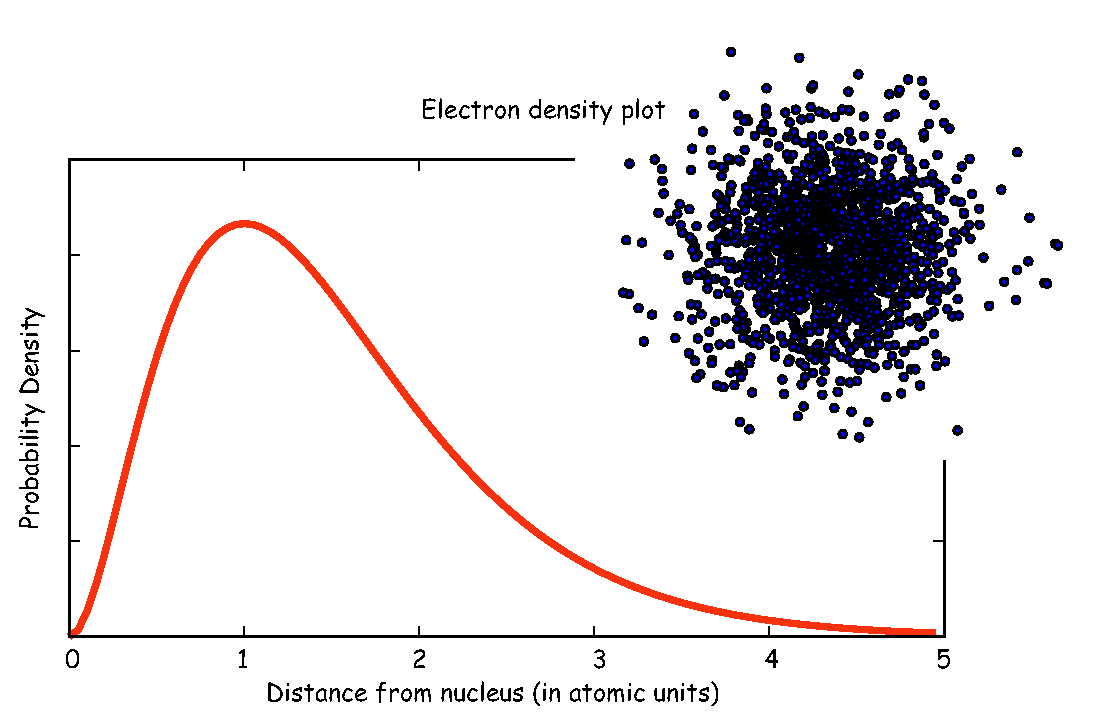
\includegraphics[width=10 cm]{EPSfiles/1s.eps}
\caption{Plot of radial distribution and ``dot-density'' for the 1s electron shell.}
\label{fig:1s}
\end{figure}

\noindent 
 Apparently, this  does not happen, so the classical approach is fatally flawed and we must turn to quantum mechanics.   


\index{quantum!mechanics}
In quantum mechanics,  electronic motion is stabilized  by the fact that electrons can only have certain energy states; they are quantized.   The energy of a given electron can be  described in terms of solutions, $\Psi$, to  something called  
\index{Schr\"odinger's wave equation}
Schr\"odinger's 
wave equation. The function $\Psi(r,\theta,\phi)$ gives the probability  of finding an electron at a given position.   [Remember from Chapter  2 that $r,\theta,\phi$ are the three spherical coordinates.]    It depend on three special
\index{quantum!numbers}
{\it quantum numbers} ($n,l,m$):

\beq
\Psi_{r,\theta,\phi} = R_n^l(r) Y_l^m(\phi,\theta),
\label{eq:wave}
\eeq

\noindent The number $n$ is the so-called ``principal'' quantum number. The $R_n^l(r)$ are functions specific to the element in question and the energy state of the electron $n$.  It is evaluated at an   effective radius $r$ in atomic units.  The $Y_l^m$ are a fully normalized complex representation of the spherical harmonics introduced in Section~\ref{sect:igrf}.     
For each level $n$, the  number $l$ ranges from 0 to $n$-1 and  $m$ from $l$ backwards to $-l$.  

 The lowest energy of the quantum wave equations is found by setting  $n$ equal to unity and both $l$ and $m$ to zero.   Under these conditions, the solution to the wave equation is given by:
 $$
R_{1,0} = 2  Z^{3\over 2}  e^{-\rho/2},
$$
\beq
Y_{0,0}=  ({1\over {4\pi}})^{1\over 2}
\eeq
\noindent where $Z$ is the atomic number and $\rho$ is $2Zr/n$.  Note that at this energy level, there is no dependence of $Y$ on $\phi$ or $\theta$.  Substituting these two equations into Equation~\ref{eq:wave} gives  the probability density  $\Psi$ for  an electron as a function of radius of $r$.  This  is sketched as the line in Figure~\ref{fig:1s}.   Another representation of the same idea is shown in the inset, whereby the density of dots at a given radius reflects the probability distribution shown by the solid curve.  The highest dot density is found at a radius of about one atomic unit, tapering off the farther away from the center of the atom.   Because there is no dependence on $\theta$ or $\phi$ the probability distribution  is a spherical 
\index{electronic!shells}
shell.    All the $l,m=0$ shells are spherical and are often referred to as the 1s, 2s, 3s shells, where the numbers are the energy levels $n$.   A surface with equal probability is a sphere and example of one such shell is shown in Figure~\ref{fig:shells}a.  

For $l=1$, $m$ will have values of -1, 0 and 1 and the $Y_l^m(\phi,\theta)$s are given by:

$$
Y_1^{-1}= {1\over2} \sqrt{{3\over {2\pi}}}\sin\theta e^{-i\phi}, \hskip 1em Y_1^{0}= {1\over2} \sqrt{{3\over {\pi}}}\cos\theta,  \hskip 1em  Y_1^{1}= {-1\over2} \sqrt{{3\over {2\pi}}}\sin\theta e^{i\phi}.
$$
\noindent Shells with $l=1$ depend not only on radial distance but also on the angles $\phi$ and $\theta$, so they are not spheres, but more complicated shapes.  A surface of equal probability for one such shell (the $m=1$ shell) is shown in Figure~\ref{fig:shells}b.  Shells with $l=1$ are called the  ``p'' shells.  

As might be expected,  the shells for  $l=2$ are even more complicated that for $l=1$.  These shells are called   ``d'' shells and two examples are shown in Figure~\ref{fig:shells}c and d.    




\begin{figure}[h!tb]
%\epsfxsize 13cm
%\centering \epsffile {EPSfiles/shells.eps}
\centering  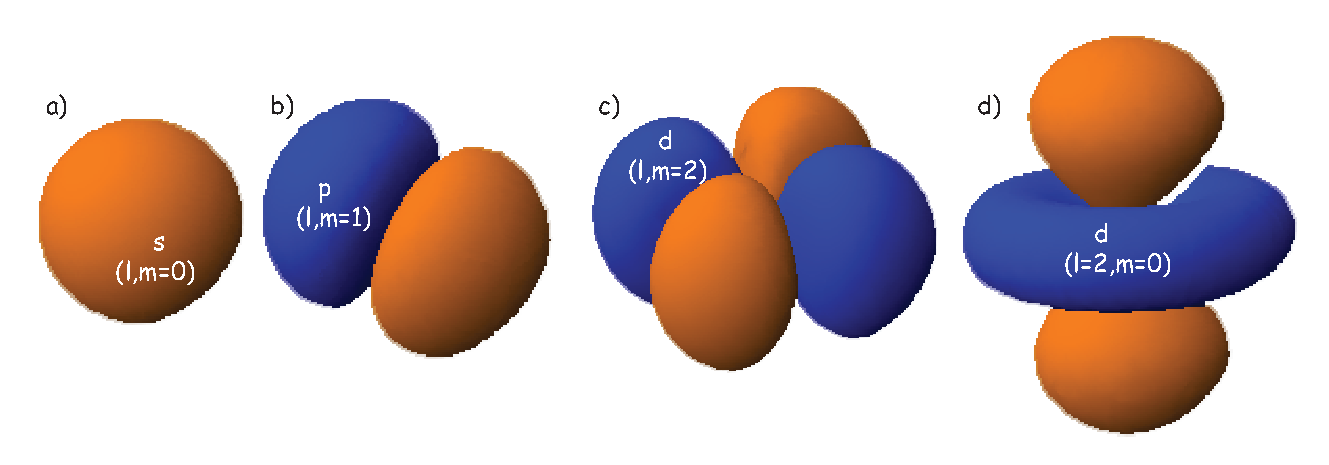
\includegraphics[width=13 cm]{EPSfiles/shells.eps}
\caption{Examples of surfaces of equal probability of the first three shells ($l=1,2,3$).   Surfaces created with Orbital Viewer.    }
\label{fig:shells}
\end{figure}


Returning to the tiny circuit idea,  somehow the motion of the electrons in their shells acts like an electronic circuit and creates a \index{magnetic!moment}
magnetic moment.  
In quantum mechanics,  the angular momentum vector of the electron ${\bf L}$  is quantized, for example as integer multiples of $\hbar$, the 
``reduced'' 
\index{Planck's constant}
Planck's constant (or ${h\over{2\pi}}$ where $h$ = 6.63 x 10$^{-34}$ Js).   The magnetic moment arising from the orbital angular momentum is given by:
$$
|\m| = -{ {q_e}\over {2\mu_e}}|{\bf L}|,
$$
\noindent
where $\mu_e$ is the mass of an electron (9.11 x 10$^{-31}$ kg), $q_e$= -1.69 x 10$^{-19}$C.   The smallest value of ${\bf L}$ is $\hbar$ so 
 the fundamental
unit of magnetic moment arising from the oribit of  electrons is given by:

\beq
|\m_b| = { \hbar 
{q_e}\over {2\mu_e}
} = 9.27 \cross 10^{-24} 
{{\hbox{kg  m}^2}\over {\hbox{s}}}
 \cdot
 {\hbox{C}\over {\hbox{kg}}}
 = 9.27 \cross 10^{-24} {\hbox{Am}^2}.
\label{eq:bohrmagneton}
\eeq

\noindent This is known as  the 
\index{Bohr magneton}
{\it Bohr magneton}.   

\begin{figure}[h!tb]
%\epsfxsize 9cm
%\centering \epsffile{EPSfiles/structure.eps}
\centering  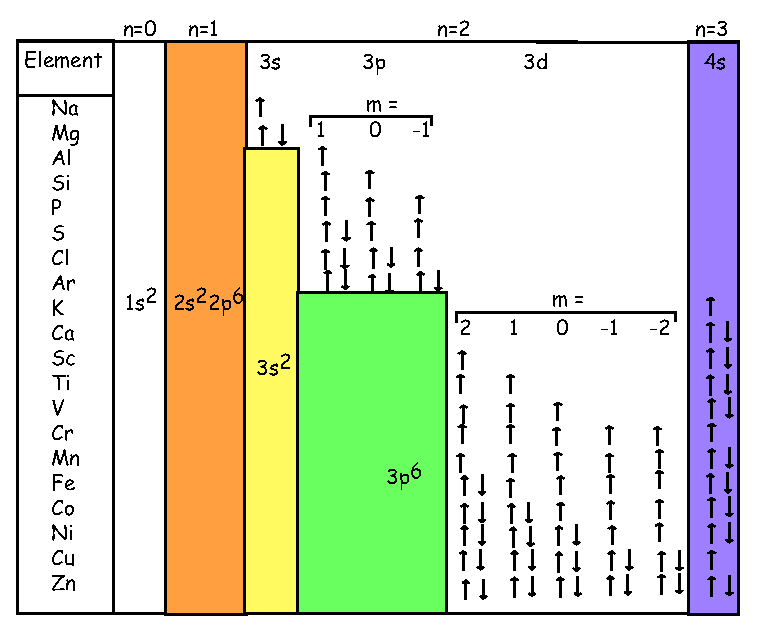
\includegraphics[width=9 cm]{EPSfiles/structure.eps}
\caption{Electronic structure of elements from Na to Zn. }
\label{fig:structure}
\end{figure}


So far we have not mentioned one last quantum number, $s$.  This is the 
\index{electronic!spin}
``spin'' of the electron and has a value of $\pm {1\over 2}$.   The spin itself produces a magnetic moment which is given by $2sm_b$, hence is numerically identical to that produced by the orbit.   

Atoms have the same number of electrons as protons in order to preserve charge balance.  Hydrogen has but one lonely electron which in its lowest energy state sits in the $1s$ electronic shell.  Helium has a happy pair, so where does the second electron go?  To fill in their electronic shells, atoms follow three rules:

\begin{enumerate}

\item No two electrons may have the same set of quantum numbers.  This is 
\index{Pauli's exclusion principle}
Pauli's exclusion principle.  Because spin ($s$) can be $\pm {1\over 2}$, two  electrons fit in one orbital.    When a single electron occupies a given orbital, it is called ``unpaired'' and has a magnetic moment of 1 $m_b$.  

\item Orbitals are filled in order of increasing energy.  The energy state of a given orbital is dependent on the context (whether the atom is bound to other atoms or not), but in general they will be filled according to the scheme shown in Figure~\ref{fig:structure}.  

\item Electrons are added so that the  spins remain as parallel as possible 
\index{Hund's rule}
(Hund's rule).   Notice in  Figure~\ref{fig:structure} that when filling the third energy level ($n=3$), all five $d$ shells  are filled with one kind of spin (say, all up, or +$1\over 2$), before the electrons begin to pair up.  Also, because the energies of the shells change somewhat according to the context they are in, the 4$s$ shell will actually give up an electron to a $d$ shell, before the $d$ shells begin to pair up.    Hund's rule gives the atoms with some $d$ shell electrons (the so-called ``transition elements'', e.g.,  Cr, Mn, Fe, Co and Ni)  the possibility of large magnetic moments.    

\end{enumerate}


Each unpaired spin has a moment of one 
\index{Bohr magneton}
Bohr magneton $m_b$. 
  The elements with the most unpaired spins are the transition elements which  are responsible for 
most of the paramagnetic behavior observed in rocks.     For example, in  Figure~\ref{fig:structure} we see that Mn has a structure of: ($1s^22s^22p^63s^23p^6) 3d^54s^2$, hence has five unpaired spins and a net moment of 5 $m_b$.   Fe  has a structure of ($1s^22s^22p^63s^23p^6) 3d^6 4s^2$ with a net moment of 4 $m_b$,  In minerals, the transition elements are in a variety of oxidation states.  Fe commonly occurs as Fe$^{2+}$ and Fe$^{3+}$.  When losing electrons to form ions, transition metals lose the 4s electrons first, so we have for example, Fe$^{3+}$ with a structure of ($1s^22s^22p^63s^23p^6) 3d^5$, or 5 $m_b$.  Similarly Fe$^{2+}$ has 4 $m_b$ and Ti$^{4+}$ has no unpaired spins.  Iron is the main magnetic species in geological materials, but Mn$^{2+}$ (5 $m_b$) and Cr$^{3+}$ (3 $m_b$) occur in trace amounts.  




\section{Induced magnetization}  

\index{magnetization!induced}
\index{induced magnetization}

We have learned that there are two sources of magnetic moments in electronic motions:  the orbits and the (unpaired)  spins.      These moments respond to external magnetic fields giving rise to an induced magnetization, a phenomenon alluded to briefly in Chapter 1.  We will consider first the contribution of the 
\index{electronic!orbit}
electronic orbits. 

\begin{figure}[htb]
%\epsfxsize 2in
%\centering \epsffile{EPSfiles/larmor.eps}
\centering  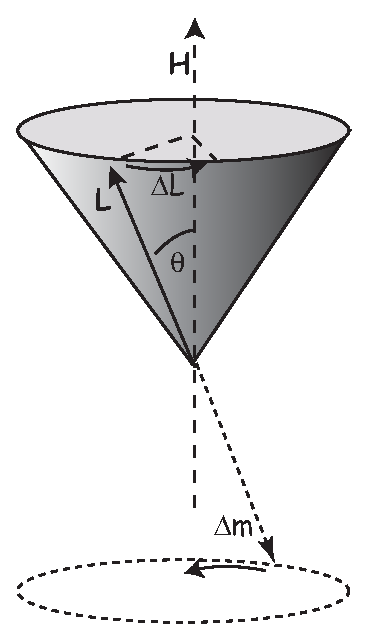
\includegraphics[width=2 in]{EPSfiles/larmor.eps}
\caption{Larmor precession.  The orbit of the electron has an angular momentum vector ${\bf L}$ which creates a magnetic moment.  In the presence of a magnetic field $\H$, the moment experiences a torque which causes a change in angular momentum $\Delta L$.  The precession of the electronic orbit about $\H$ creates an induced magnetic moment $\Delta m$ in a sense opposite to the applied field $\H$.}
\label{fig:larmor}
\end{figure}

\subsection{Orbital contribution and diamagnetism}
\label{sect:dia}


The   angular momentum of  electrons is quantized  in magnitude but also has direction (see  ${\bf L}$ in Figure~\ref{fig:larmor}).  The angular momentum  vector has an associated magnetic moment vector $\m_b$.  A magnetic field $\H$ exerts  a torque on the moment, which nudges it (and the momentum vector associated with it)  to the side ($\Delta L$).  ${\bf L}$  therefore will  precess around the magnetic field direction, much like a spinning top precesses around the direction of gravity.  The precession of ${\bf L}$ is called 
\index{Larmor precession}
{\it Larmor precession}.  

 The changed momentum vector from Larmor precession  in turn results in a   changed
magnetic moment vector $\Delta m$.   The sense of the change in net moment is always to oppose the applied field.
Therefore, the response of  the magnetic moments of electronic orbitals creates an induced magnetization $\M_I$ that is observable outside
the substance;  it is related to the applied field by: 

$$
\M_I=\chi_d \H.
$$

\noindent 
We learned in Chapter 1 that the proportionality between induced magnetization and the applied field    is known as the  
\index{magnetic!susceptibility}%
{\it magnetic susceptibility}.
The ratio $\M_I/\H $ for the response of the electronic orbitals is  termed the 
\index{magnetic!susceptibility!diamagnetic}
\index{diamagnetism}
{\it diamagnetic susceptibility\/} $\chi_d$;  it is negative, 
essentially temperature independent and quite small. This diamagnetic
response is a property of all matter, but for substances whose atoms possess atomic magnetic moments,
diamagnetism is swamped by effects of magnetic fields on the atomic magnetic moments.
  In the absence of unpaired electronic spins, diamagnetic susceptibility dominates the  magnetic response.  Common diamagnetic substances include quartz (SiO$_2$), calcite (CaCO$_3$) and water (H$_2$O).   The mass normalized susceptibility of  quartz is -0.62 x 10$^{-9}$ m$^3$kg$^{-1}$ to give you an idea of the magnitudes of  these things. 

\begin{figure}[htb]
%\epsfxsize 13.5cm
%\centering \epsffile{EPSfiles/para.eps}
\centering  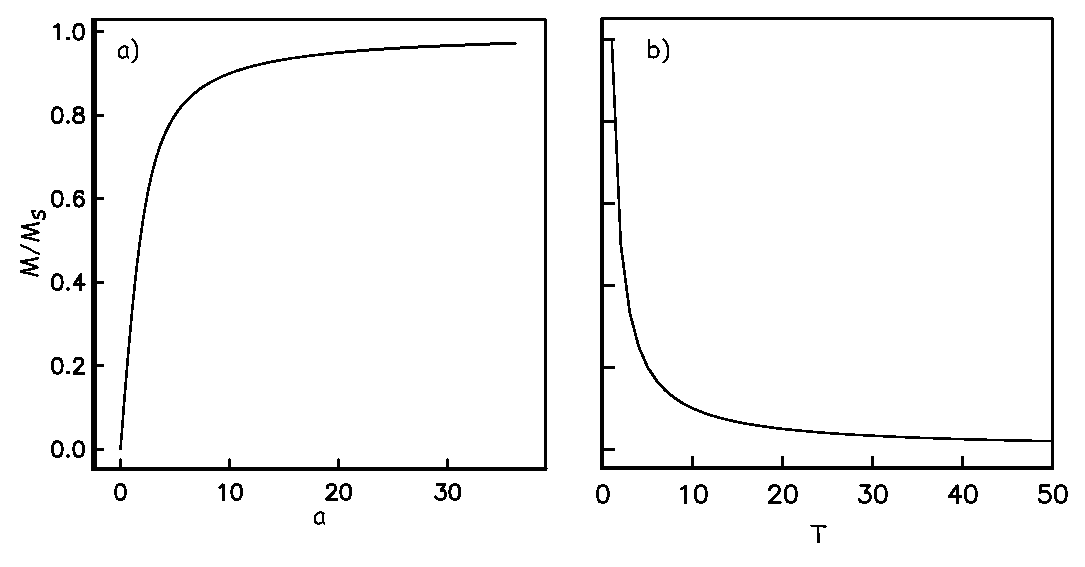
\includegraphics[width=13.5 cm]{EPSfiles/para.eps}
\caption{a) Paramagnetic magnetization (obtained from the Langevin function $\mathcal{L}(a)$ versus $a= mB/kT$.)  b) Paramagnetic magnetization as a function of temperature (Curie Law).}
\label{fig:para}
\end{figure}


\subsection {Role of electronic spins and paramagnetism}
\label{sect:para}

In many geological materials, the orbital contributions cancel out because they are randomly oriented with respect to one another and the magnetization arises from the electronic spins.    We mentioned that unpaired electronic spins  behave as magnetic dipoles with a moment of one 
\index{Bohr magneton}
Bohr magneton. 
In the absence of an applied field, or in  the absence of the  
ordering influence of neighboring
spins which are known as 
\index{exchange!interactions}%
{\it exchange interactions}, the electronic spins are essentially randomly oriented. 
An applied field acts to align the
spins which creates a net magnetization equal to $\chi_p H$ where  
\index{paramagnetism}%
\index{magnetic!susceptibility!paramagnetic}
$\chi_p$ is the {\it paramagnetic susceptibility}.  For
any geologically relevant conditions, the induced magnetization is linearly dependent on the applied field. In paramagnetic solids, atomic magnetic moments react independently to applied magnetic fields and to
thermal energy. At any temperature above absolute zero, thermal energy vibrates the crystal lattice, causing
atomic magnetic moments to oscillate rapidly in random in orientations. In the absence of an applied
magnetic field, atomic moments are equally distributed in all directions with  a resultant magnetization of zero.


A useful first order model for  paramagnetism was worked out by 
\index{Langevin!theory}
P. Langevin in 1905.   (Of course in messy reality things are a bit more complicated, but Langevin theory will work well enough for us at this stage.)
Langevin theory is based on a few simple
premises:


\begin{enumerate}

\item Each unpaired spin contributes a dipole moment. 

\item In the absence of an applied
field, the moments are essentially randomly oriented, \ie
all directions are equally likely to occur.

\item Application of a magnetic field exerts an aligning torque  on the atomic magnetic moments.  The 
\index{magnetic!energy}
magnetic energy $E_m$ (see also Section~\ref{sect:Me} in Chapter 1)  of a 
\index{magnetic!moment}
magnetic moment $\m$ at an angle $\theta$ with an external magnetic
 field $\B=\mu_o \H$ is given by:


\beq
E_m = -\m \cdot \B = -mB  \cos \theta.
\label{eq:Em}
\eeq



 Magnetic energy is at a minimum when the
magnetic moment is lined up with the magnetic field.  

\item There is  competition between the 
\index{magnetic!energy}
magnetic energy $E_m$ and the 
\index{energy!thermal}
 thermal energy $kT$ 
 where $k$ is 
\index{Boltzmann's!constant}
Boltzmann's constant (1.38 x 10$^{-23}$ m$^2$ kg s$^{-2}$ K$^{-1}$) and $T$ is
temperature in kelvin).
\end{enumerate}

Consider an atomic magnetic moment, ($m$ = 2$m_b$ = 1.85$\cross 10^{-23}$
Am$^2$), in a magnetic field of 10$^{-2}$ T, (for reference, the largest  geomagnetic field at the surface is about 65 $\mu$T -- see Chapter 2). The aligning energy is therefore 
$mB$ = 1.85 $\cross$ 10$^{-25}$ J). However, thermal energy at 300K
(traditionally chosen as a temperature close to room temperature providing easy arithmetic) is 
Boltzmann's constant  times the temperature,  or  about  4 x 10$^{-21}$ J.   So thermal energy is several orders of magnitude larger than the
aligning energy and  the net magnetization is small even in this rather large (compared to the Earth's field) magnetizing field.




Using the principles of 
\index{statistical mechanics}
statistical mechanics, we find that the
probability  density of a particular magnetic moment having a 
\index{magnetic!energy}
magnetic energy of  $E_m$ is given by:

\beq
P(E) \propto \exp (-E_m/kT).
\label{eq:PE}
\eeq

\noindent From this we see that the degree of alignment depends exponentially on the ratio of magnetic energy to thermal energy.  The degree of alignment with the magnetic field controls the net magnetization $M$.  When spins are completely aligned, the substance has a
\index{magnetization!saturation}
 {\it saturation magnetization} $M_s$.  The probability density function leads directly to the following relation (derived in  Appendix~\ref{app:langevin}): 

\beq
{M\over {M_s}} =
{ [\hbox{coth }a -
{
1\over{a}
}]=\mathcal{L}(a).
}
\label{eq:Lang} 
\eeq

\noindent where  $a=mB/kT$. The function enclosed in square brackets is known as the 
\index{Langevin!function}
{\it Langevin function} ($\mathcal{L}$).


Equation~\ref{eq:Lang} is plotted in   Figure~\ref{fig:para}a and predicts several intuitive results: 1) $M = 0$ when $B=0$ and 2) $M/M_s = 1$ when the applied  magnetic field is infinite. Furthermore,   $M$  is some 90\% 
of $M_s$ when $mB$ is some 10-20 times $kT$. 
When $kT>> mB, \mathcal{L}(a)$ is approximately linear with a slope of
$\sim 1/3$.  At room temperature and fields up to many tesla, 
$\mathcal{L}(a)$ is approximately $ mB/3kT$. 
\index{paramagnetic susceptibility!low-field}%
If the moments  are unpaired spins ($m=m_b$), then the maximum magnetization possible ($M_s$) is given by the number of moments $N$,  their magnitude ($m_b$) normalized by the volume of the material $v$ or  $M_s=Nm_b/v$,
and

$$
{M\over{M_s}} \simeq {
{ m_b \mu_o }\over
{3kT}
}
H .
$$

Please note that we have neglected all deviations from isotropy including quantum
mechanical effects as well as crystal shape, lattice defects, and state
of stress. These complicate things a little, but to first order the treatment followed here provides  a good approximation.  
We can rewrite the above equation as:


\beq
{M\over H} = {{m_b\mu_o}\over {3kT}}\cdot M_s =
{{Nm_b^2\mu_o}\over{3kv}}\cdot {1\over T} = \chi_p.
\eeq

 To first order,
 paramagnetic susceptibility $\chi_p$ is positive, 
larger than diamagnetism and inversely proportional to temperature.
This inverse T dependence (see Figure~\ref{fig:para}b)  is known as 
\index{Curie's Law}
Curie's law of
paramagnetism.  The paramagnetic susceptibility of, for example, biotite is 790 x 10$^{-9}$ m$^3$ kg$^{-1}$, or about three orders of magnitude larger than quartz (and of the opposite sign!).  


We have considered the simplest case here in which  $\chi$ can be treated as 
a scalar and is referred to as  the
\index{magnetic!susceptibility!bulk}%
{\it bulk magnetic susceptibility} $\chi_b$.
In detail, magnetic susceptibility can be quite complicated. 
The relationship
between induced magnetization and applied field can be
affected by crystal shape, lattice
structure, dislocation density, state of stress, etc., 
which give rise to possible anisotropy of the susceptibility.
Furthermore, there are only a finite number of electronic moments within
a given volume.  When these are fully aligned, the magnetization reaches
saturation.  Thus, magnetic susceptibility is both anisotropic and non-linear
with applied field.

\begin{figure}[htb]
%\epsfxsize 10cm
%\centering \epsffile{EPSfiles/exchange.eps}
\centering  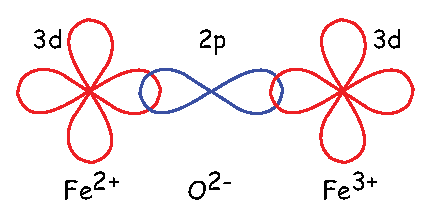
\includegraphics[width=10 cm]{EPSfiles/exchange.eps}
\caption{ Exchange energy associated with overlapping orbitals.  Example of super-exchange between the $3d$ orbitals of two iron cations through the $2p$ orbitals of the intervening oxygen anion.  The  two electrons in the $2p$ shells are, by necessity antiparallel.  These are shared by the $3d$ shells, hence the two cations have anti-parallel spins. [Figure redrawn from O'Reilly, 1984.]}
\label{fig:exchange}
\end{figure}


\section {Ferromagnetism}
\label{sect:ferro}

Some substances give rise to a magnetic field in the absence of an applied field. 
This magnetization  is called {\it remanent } or
\index{magnetization!spontaneous}%
 {\it spontaneous} magnetization, also   loosely known as
\index{ferromagnetism}%
{\it ferromagnetism (sensu lato)}. 
 Magnetic remanence is caused by
strong interactions between neighboring spins that occur in certain
crystals.  

The so-called
\index{exchange!energy}%
{\it exchange energy} is minimized when the spins
are aligned parallel or anti-parallel depending on the details of the crystal
structure.  
Exchange energy is a consequence of the Pauli exclusion principle (no two electrons can have the same set of quantum numbers).  
In the transition elements, the $3d$ orbital is particularly 
susceptible to exchange interactions because of
its shape and the prevalence of unpaired spins, 
 so remanence is characteristic of
certain crystals containing transition elements with unfilled {$ 3d$} orbitals.  

In oxides, oxygen can form a bridge between neighboring cations which are otherwise too far apart for direct overlap of the $3d$ orbitals in a phenomenon known as superexchange.  In Figure~\ref{fig:exchange} the $2p$ electrons of the oxygen are shared with the neighboring $3d$ shells of the iron ions.  Pauli's exclusion principle means that the shared electrons must be antiparallel to each of  the electrons in the $3d$ shells.  The result is that the two cations are coupled.  In the case shown in Figure~\ref{fig:exchange} there is an Fe$^{2+}$ ion coupled antiparallel to an Fe$^{3+}$ ion.  For two ions with the same charge, the coupling will be parallel.  Exchange energies are huge, equivalent to the energy associated with the same moment in  a field of the order of 1000 T.  [The largest field available in the Scripps paleomagnetic laboratory is about 2.5 T, and that only fleetingly.]
 

 
As temperature increases,  crystals expand and exchange  becomes weaker.
 Above a temperature characteristic of
 each crystal type (known as the
 \index{Curie temperature}
  {\it Curie temperature}
 $T_c$), cooperative spin  behavior disappears entirely and the material becomes 
paramagnetic.  

 
\begin{figure}[htb]
%\epsfxsize 12cm
%\centering \epsffile{EPSfiles/MsT.eps}
\centering  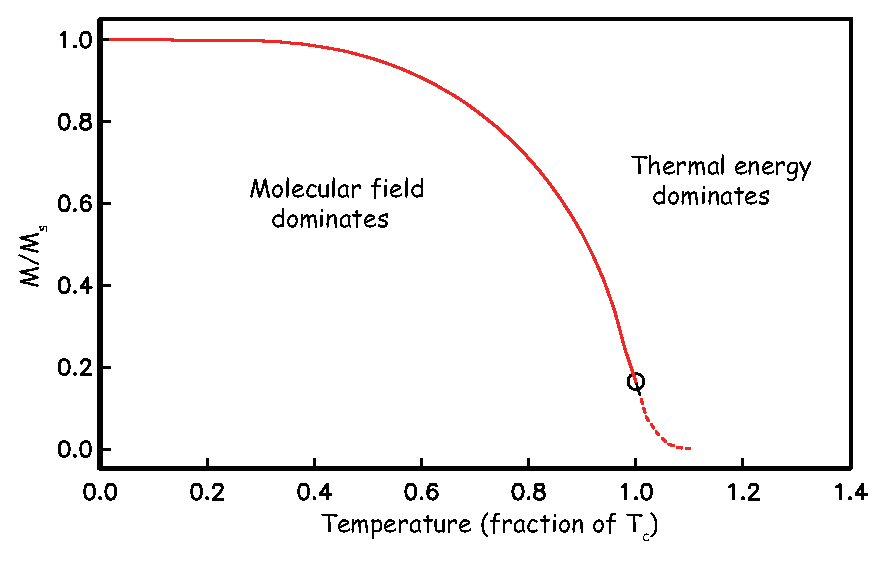
\includegraphics[width=12 cm]{EPSfiles/MsT.eps}
\caption{Behavior of magnetization versus temperature of a ferromagnetic
substance.  Below $T_c$, the magnetization follows Equation 3.9 and is the ferromagnetic magnetization.  Above $T_c$  the magnetization follows Equation 3.8 and is the induced magnetization. [Redrawn from Tauxe, 1998.]  }
\label{fig:MsT}
\end{figure}
\nocite{tauxe98}

While the phenomenon of ferromagnetism results from complicated
interactions of neighboring spins, it is useful to think of the
ferromagnetic moment as resulting from a quasi-paramagnetic response to
a huge internal field.  This imaginary field is termed the 
\index{Weiss molecular field}
{\it Weiss molecular field} $H_w$.  In 
Weiss theory, $H_w$ is proportional to the
magnetization of the substance, i.e., 

$$
H_w = \beta M,
$$

\noindent
where $\beta$ is the constant of proportionality.
The total magnetic field that the substance experiences is:

$$
H_{tot} = H + H_w = H + \beta M,
$$

\noindent where $H$ is the external field.  By analogy to paramagnetism,
we can substitute $a=\mu_om_b(H_{tot})/kT)$ for $H$ in
\index{Langevin!function}
 Langevin function:

\beq
{M  \over {M_s}} {= \mathcal{L} \left({ {\mu_o m_b(H+\beta M)}\over{kT} } \right)}.
\label{eq:Mweiss}
\eeq

\noindent For temperatures above the Curie temperature $T_c$ (i.e.
$T-T_c>0$) there is by definition no internal field, hence  $\beta M$  is zero.
Substituting $N m_b/v$ for $M_s$, and using the low-field approximation
for $\mathcal{L} (a)$, Equation~\ref{eq:Mweiss} can 
be rearranged to get:

\index{Curie-Weiss law}%
\beq
{M\over H} = { {\mu_o N m_b^2}\over {v3k(T-T_c)} } \equiv \chi_f.
\label{eq:curieweiss}
\eeq

\noindent
Equation~\ref{eq:curieweiss} is known as the Curie-Weiss law and governs
ferromagnetic susceptibility above the Curie temperature (dashed line in Figure~\ref{fig:MsT}). 

\begin{figure}[htb]
%\epsfxsize 11cm
%\centering \epsffile{EPSfiles/curie.eps}
\centering  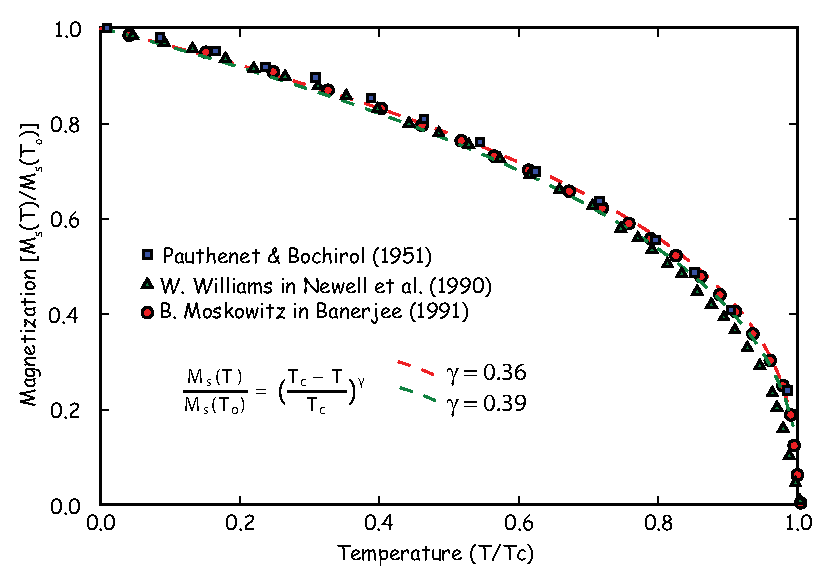
\includegraphics[width=11 cm]{EPSfiles/curie.eps}
\caption{Various data sets for  the behavior of $M_s(T)$ for magnetite.     }
\label{fig:curie}
\end{figure}
\nocite{pauthenet51,newell90,banerjee91}

Below the Curie temperature $H_w>>H$;  we can neglect the external field $H$  and 
get:


$$
{M\over {M_s}} = \mathcal{L}  \bigl( {{\mu_o m_b \beta M}\over{kT}}\bigr).
$$ 

\noindent Substituting again for $M_s$ and rearranging, we get:


\beq
{M\over M_s} = \mathcal{L} \bigl( {{Nm_b^2 \beta}\over{vkT}}\cdot {M\over M_s}
\bigr) =
\mathcal{L}  \bigl( {T_c \over T} \cdot {M\over M_s} \bigr),
\label{eq:Mferro}
\eeq
\index{Curie temperature}%
\noindent where $T_c$ is the Curie temperature and is given by:
$$T_c = { {Nm_b^2 \beta}\over{vk}}.$$
\noindent  
Equation~\ref{eq:Mferro} can be solved graphically or
numerically and is sketched (solid line)  in Figure~\ref{fig:MsT}.  Below the Curie
temperature, exchange interactions are strong relative to the
external field and  the magnetization is
governed by Equation~\ref{eq:Mferro}. Above the Curie temperature, it
follows the Curie-Weiss law (Equation~\ref{eq:curieweiss}).  




We have treated ferromagnetism from a classical point of view and this is strictly incorrect because ferromagnetism  results primarily from quantum mechanical phenomena.  The primary difference  between the classical derivation and the quantum mechanical one lies in the fact that in quantum mechanics, only certain angles of the magnetic moments are allowed, as opposed to all directions in Langevin theory.  In the end, the predictions of magnetization as a function of temperature are different in detail.   The end product of the quantum mechanical treatment 
\index{Dunlop, D.J.}
\index{\"Ozdemir, \"O.}
(see Dunlop and \"Ozdemir, 1997) \nocite{dunlop97} is that the variation of 
\index{magnetization!saturation}
saturation magnetization as a function of temperature can be reasonably well approximated (near the
\index{Curie temperature}
 Curie Temperature, $T_c$) by a normalized power law variation:
\begin{equation}
{M_s(T)\over {M_s(T_o)}} = \bigl[{  {T_c - T}\over{T_c-T_o}} \bigr]^{\gamma },
\label{eq:MsT}
\end{equation}

\noindent  where  $\gamma$ is 0.5 from simple molecular field theory and $T_o$ is absolute zero (in kelvin).   Dunlop and \"Ozdemir (1997) cite a value of around 0.43 for $\gamma$, but the  data sets cited by Dunlop and \"Ozdemir (1997; e.g., Figure 3.5 on page 52) are actually best-fit with values for $\gamma$ of about 0.36 -- 0.39 (see Figure~\ref{fig:curie}).   These curves have been normalized by their inferred curie Temperatures which are around 565$^{\circ}$C (data of B. Moskowitz, cited in
\index{Banerjee, S.K.}
 Banerjee, 1991).  \nocite{banerjee91} 

\begin{figure}[h!tb]
%\epsfxsize 14cm
%\centering \epsffile{EPSfiles/spins.eps}
\centering  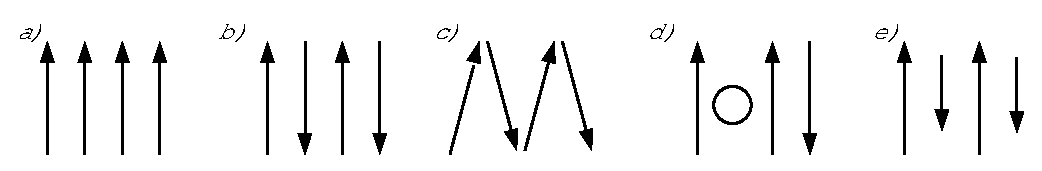
\includegraphics[width=14 cm]{EPSfiles/spins.eps}
\caption{Types of spin alignment in ferromagnetism {\it (sensu lato)}:
a) ferromagnetism ({\it sensu stricto}), b) antiferromagnetism, c)
spin-canted antiferromagnetism, d) defect anti-ferromagnetism, e)
ferrimagnetism.
}
\label{fig:spins}
\end{figure}



\index{ferromagnetism}%

As we have seen,
below the Curie temperature, certain crystals have a permanent
(remanent) magnetization resulting from the alignment of unpaired
electronic spins over a large area within the crystal.  Spins may be
 either parallel or anti-parallel;
the sense of spin alignment is controlled
entirely by crystal structure. The energy term associated with this
phenomenon is the 
\index{exchange!energy}%
{exchange energy}. 
\index{ferromagnetism}%
\index{ferrimagnetism}%
\index{antiferromagnetism}%
 There are three categories of spin alignment: ferromagnetism ({\it
sensu stricto}),  ferrimagnetism and antiferromagnetism (see
Figure~\ref{fig:spins}).  

 \begin{figure}[htb]
 %\epsfxsize 14cm
 %\centering \epsffile{EPSfiles/spinwave.eps}
 \centering  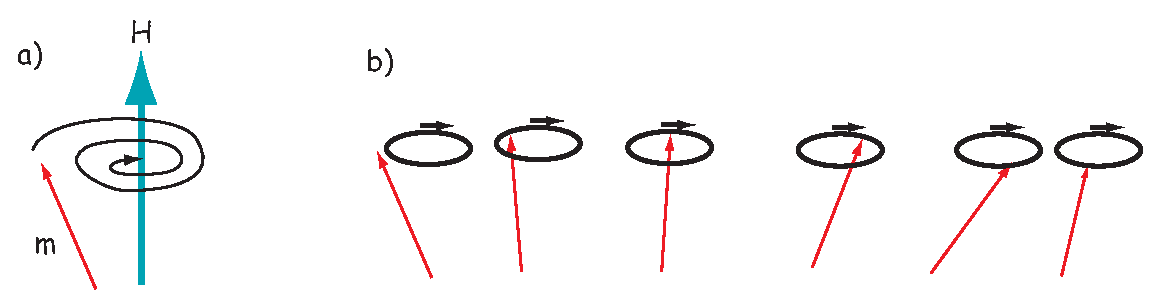
\includegraphics[width=14 cm]{EPSfiles/spinwave.eps}
 \caption{a) Response of a magnetic moment to the torque of an applied field for isolated moments.  b) Response of coupled moments to a perturbation. Neighboring spins produce an effect known as ``spin waves''.}
 \label{fig:spinwave}
 \end{figure}
 


\index{ferromagnetism}%
In {\it ferromagnetism} ({\it sensu stricto}, Figure~\ref{fig:spins}a), the
\index{exchange!energy}%
 exchange energy is minimized when all the spins
are  parallel, as occurs in  pure
\index{iron}%
iron.  When spins are perfectly
antiparallel 
\index{antiferromagnetism}%
({\it antiferromagnetism}, Figure~\ref{fig:spins}b), 
there is no net magnetic moment, as occurs
in 
\index{ilmenite}%
ilmenite.    Occasionally, the antiferromagnetic spins are not 
perfectly aligned in an  antiparallel orientation, but are canted by a 
few degrees.  This
\index{spin-canting}%
{\it spin-canting} (Figure~\ref{fig:spins}c) gives rise to
a weak net moment, as occurs in 
\index{hematite}%
hematite, a common magnetic mineral (see Chapter 6).  Also, antiferromagnetic materials can
have a net moment if spins are not perfectly compensated owing to
defects in the crystal structure, as occurs in fine-grained hematite.
The uncompensated spins result in a so-called {\it
defect} moment (Figure~\ref{fig:spins}d).   
We note in passing that the temperature at which spins become disordered
in antiferromagnetic substances is termed the 
\index{N\'eel!temperature}%
{\it N\'eel temperature}. In
\index{ferrimagnetism}%
 {\it ferrimagnetism},  spins are also aligned antiparallel, but the
magnitudes of the moments in each direction are unequal, resulting
in a net moment (Figure~\ref{fig:spins}e). 


In figures like Figure~\ref{fig:spins},  electronic spins are depicted as being simply aligned with some minimum energy  direction (aligned with the field, or along some easy axis).  Yet we already know about the paramagnetic effect of misalignment through  random thermal fluctuations.   We learned that an external magnetic field generates a torque  on the electronic spins, and in isolation, a magnetic moment will respond to the torque in a manner similar in some respects to  the way a spinning top responds to gravity: the magnetic moment will precess about the applied field direction, spiraling in  and come to a rest parallel to it (Figure~\ref{fig:spinwave}a). Because of the strong exchange coupling  in ferromagnetic phases, spins tend to be aligned parallel (or antiparallel) to one another and the spiralling is done in a coordinated fashion, with neighboring spins as parallel as possible to one another (Figure~\ref{fig:spinwave}b).   This phenomenon is known as a 
\index{spin waves}%
{\it spin wave}.  
 
 
\vskip .5 in\noindent{SUPPLEMENTAL READINGS:} O'Reilly (1984), Chapter 3.1;    \nocite{oreilly84}
Dunlop and \"Ozdemir (1997), Chapter 2.1 to 2.7.

\vskip 24pt
{{\parindent 0pt \parskip 12pt 







\section{Problems }


{\bf Problem 1}

a) Given one Bohr magneton ($m_b$) in the Earth's field (40 $\mu$T), write a program using python that calcuates magnetostatic interaction energy (-$m_bB\cos \theta$) for angles 0$\rightarrow$ 180$^{\circ}$.   Make a plot of this with the {\bf matplotlib} module in Python (see online \href{http://earthref.org/PmagPy/cookbook/#matplotlib}{PmagPy} documentation).  

b) Calculate the thermal energy at room temperature (300K).     How does this compare with the interaction energy? 

{\bf Problem 2}

Fayalite (Fe$_2$SiO$_4$) is a paramagnetic solid with magnetic susceptibility $\chi$ = 4.4 x 10$^{-4}$ (cgs units) at 0$^{\circ}$C (= 273K).  
A single crystal of fayalite has a volume of 2 cm$^{3}$.  This crystal is placed in a magnetic field, $H=10$ oe at 0$^{\circ}$C.  What is the resulting induced magnetic  moment $m$ of this crystal?  


a)  Do this problem first in cgs units.  Then convert your answer to SI using the conversion factors in Table~\ref{tab:units} in Chapter 1.

b)  Do the problem again  by first converting all the parameters into SI units.  Check your answer by converting the SI answer that you get back to cgs.  You should get the same answer (but you would be surprised how many people do this wrong).   

{\bf Problem 3}

If fayalite is placed in a magnetic field $H$= 100 oe at a temperature of 500$^{\circ}$C (= 773K), what is the resulting magnetization, $M$?   



{\bf Problem 4}

  MnS is a paramagnetic solid.  At 300K there are 4 x 10$^{28}$ molecules of MnS per m$^3$. Look up the number of unpaired spins for the cationic magnetic moment of Mn$^{2+}$  in the text and find  the paramagnetic susceptibility, $\chi$, of MnS at 300K?

{\bf Problem 5 } 

Try the examples for \href{http://earthref.org/PmagPy/cookbook/#curie.py}{\bf curie.py } in the {\bf PmagPy} software package.  What is the Curie temperature of the material?

}



%http://quantlab.bu.edu/acrosby/orbitals/dxy.html
 %DONE 7/15/18
%\customlink{Magnetic_anisotropy_and_domains}
\chapter {Magnetic anisotropy and domains}
\label{sect:anisintro}




Rocks often contain assemblages of  ferromagnetic minerals dispersed within a matrix of diamagnetic and paramagnetic minerals.  In later chapters we will be concerned with the magnetization of  these assemblages, but  here we continue our investigation of the behavior of individual particles.   
In Chapter 3 we learned that in some crystals electronic spins work in concert to create a spontaneous magnetization that remains in the absence of an external field.  The basis of paleomagnetism is that these ferromagnetic particles carry the record of ancient magnetic fields.  What allows the magnetic moments to come into equilibrium with the geomagnetic field and then what fixes that equilibrium magnetization into the rock so that we may measure it millions or even billions of years later?  We will begin to answer these questions over the next few chapters.  

We will start  with the second part of the question: what fixes magnetizations in particular directions?     A basic principle is that  ferromagnetic particles have various contributions to the magnetic energy which controls their magnetization.   No matter how simple or complex the combination of energies may become, the grain will seek the configuration of magnetization which minimizes its total energy.  The short answer to our question is that certain directions within magnetic crystals are at lower energy than others.  To shift the magnetization from one ``easy'' direction to another requires energy.  If the barrier is high enough, the particle will stay magnetized in the same direction for very long periods of time -- say billions of years.  In  this chapter we will address the causes and some of the consequences of  these energy barriers for the magnetization of rocks.  Note that in this chapter we will be dealing primarily with energy densities (volume normalized energies), as opposed to energy and will distinguish the two by the convention that energies are given with the symbol $E$ and energy densities with $\epsilon$.    

 In Chapter 6,  we will  discuss the behavior of common magnetic minerals, but to develop the general theory, it is easiest to focus on  a single mineral.  We choose here the most common one, magnetite.  It has a simple, cubic structure and has been the subject intensive study.  However, we will occasionally  introduce concepts appropriate for other magnetic minerals where appropriate.  
 
The simplest permanently magnetized  particles are quasi-uniformly magnetized.  These so-called
 \index{magnetic!domains}%
\index{single domain}%
 {\it single domain} (SD)
particles  have spins that act in concert,  staying as parallel (or anti-parallel) as possible.  As particles get larger, the external energy can be  minimized by allowing neighboring spins to diverge somewhat from strict parallelism; these particles are referred to as {\it pseudo-single domain} or PSD.
  \index{pseudo-single domain}
    Eventually, the spins organize themselves into regions with quasi-uniform magnetization (magnetic domains)
  \index{multi-domain}%
\index{magnetic!domains}%
separated by domain walls and are called {\it multi-domain} (MD)  particles.   These more complicated spin structures are very difficult to model and most paleomagnetic theory is based on the single domain approximation.  Therefore we begin with a  discussion of the energies of uniformly magnetized (single-domain) particles.  

\begin{figure}[htb]
%\epsfxsize 15cm
%\centering \epsffile{EPSfiles/magnetite.eps}
\centering  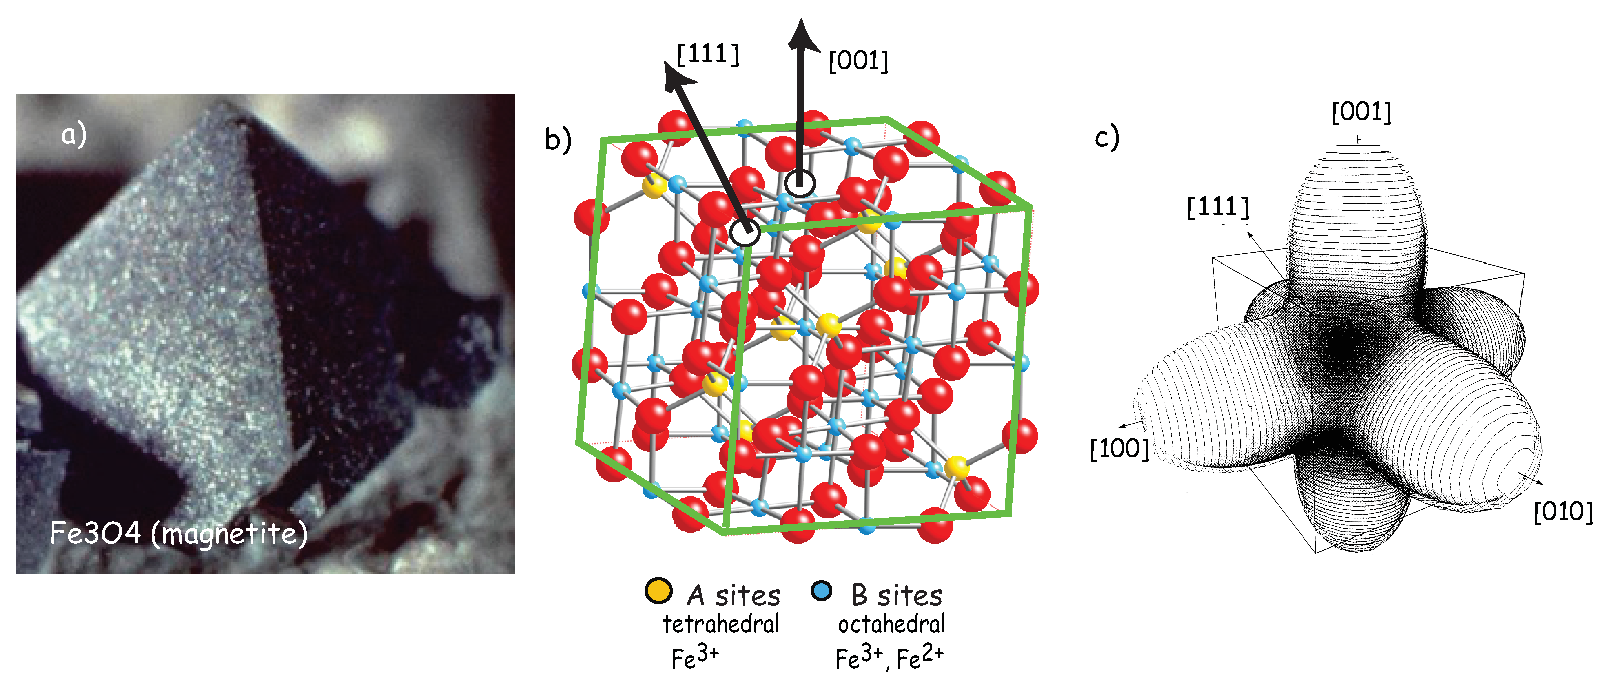
\includegraphics[width=15 cm]{EPSfiles/magnetite.eps}
\caption{a) A magnetite octahedron. [Photo of Lou Perloff in The Photo-Atlas of Minerals.]  b) Internal crystal structure.  Directions of the body diagonal ([111] direction) and orthogonal to the cubic faces ([001] direction)  are shown as arrows.   Big red dots are the oxygen anions.  The blue dots are iron cations in octahedral coordination and the yellow dots are in tetrahedral coordination.  Fe$^{3+}$ sits on the A sites and Fe$^{2+}$ and Fe$^{3+}$ sit on the B sites. c) Magnetocrystalline anisotropy energy as a function of direction within a  magnetite  crystal at room temperature.  The easiest direction to magnetize (the direction with the lowest energy -- note dimples in energy surface) is along the body diagonal (the [111] direction). [Figure from Williams and Dunlop, 1995.]    }
\label{fig:magnetite}
\end{figure}
\nocite{williams95}


 
\section{The magnetic energy of particles}


\index{magnetic!energy!exchange}
\subsection {Exchange energy}
\label{sect:exchange}

We learned in Chapter 3 that some crystalline states are capable of ferromagnetic behavior because of quantum mechanical considerations. Electrons in neighboring orbitals in certain crystals ``know" about each other's spin states.  In order to avoid  sharing the same orbital with the same spin (hence having the same quantum numbers -- not allowed by Pauli's exclusion principle), electronic spins in such crystals act in a coordinated fashion.  They will be either aligned parallel or antiparallel according to the details of the interaction.     This 
{\it exchange energy density} ($\epsilon_e$) is the source of spontaneous magnetization and is given for a pair of spins by:

$$\epsilon_e = -2J_e\S_i \cdot \S_j,
$$
\noindent where $J_e$ is the
\index{magnetic!energy!exchange!integral}
{\it exchange integral} and $\S_i$ and $\S_j$ are spin vectors.  Depending on the details of the crystal structure (which determines the size and sign of the exchange integral), exchange  energy is at a minimum when electronic spins are aligned parallel or anti-parallel.    

We define here a parameter that we will use later: the 
\index{magnetic!energy!exchange!constant}
{\it exchange constant} $A=J_eS^2/a$ where $a$ is the interatomic spacing. $A$ = 1.33 x 10$^{-11}$ Jm$^{-1}$ for magnetite, a common magnetic mineral.   

Recalling the discussion in Chapter 3, while $s$ orbitals which are spherical, the $3d$ electronic orbitals ``poke'' in certain directions.  Hence spins in  some directions within crystals  will be easier to coordinate than in others.   We can illustrate this using the example of magnetite, a common magnetic mineral (Figure~\ref{fig:magnetite}a).  
\index{magnetite}
Magnetite octahedra (Figure~\ref{fig:magnetite}a), when viewed at the atomic level (Figure~\ref{fig:magnetite}b) are composed of one ferrous (Fe$^{2+}$)  cation, two ferric (Fe$^{3+}$) cations  and four O$^{2-}$ anions.  Each oxygen anion shares an electron with two neighboring cations in a covalent bond.  

   In Chapter 3 we mentioned that in some crystals, spins are aligned anti-parallel, yet there is still a net magnetization, a phenomenon we called
   \index{ferrimagnetism}
ferrimagnetism.  This can arise from the fact that not all cations have the same number of unpaired spins.  Magnetite, with its  ferrous (4 $m_b$) and ferric (5 $m_b$) states is a good example.   There are three iron cations in a magnetite crystal giving a total of 14 $m_b$ to play with.    Magnetite is very magnetic, but not that magnetic!   From Figure~\ref{fig:magnetite}b we see that the ferric ions all sit on the tetrahedral (A) lattice sites and there are equal numbers of ferrous and ferric ions sitting on the octahedral (B) lattice sites.  The unpaired spins of the cations in the A and B lattice sites are aligned anti-parallel to one another because of \index{superexchange}
superexchange (Chapter  3)  so we have 9 $m_b$ on the B sites minus 5 $m_b$ on the A sites for a total of 4 $m_b$ per unit cell of magnetite.  




   
   \subsection {Magnetic moments and external fields}

We know from experience that there are energies associated with magnetic fields.  Just as a mass has a potential energy when it is placed in the gravitational field of another mass, a magnetic moment has an energy when it is placed in a magnetic field.  We have seen this energy briefly in Sections~\ref{sect:Me} and Equation~\ref{eq:Em}.  This energy has many names  (magnetic energy, magnetostatic energy, Zeeman energy, etc.).  Here we will work with  the  volume normalized  {\it magnetostatic interaction energy density} ($\epsilon_m$).  This energy density essentially represents the interaction between the magnetic lines of flux and the magnetic moments of the electronic spins.  It is  energy that aligns magnetic compass needles  with the ambient magnetic field.  We find the  volume normalized form (in units of Jm$^{-3}$) by  substituting  $|\M|=|\m|v^{1\over2}$ (see Chapter 1) into Equation~\ref{eq:Em}:

\begin{equation}
\epsilon_m = - \M \cdot \B.
\label{eq:Em1}
\end{equation}

\noindent 
 $\epsilon_m$  is at a minimum when the magnetization $\M$ is aligned with the field $\B$.    Single-domain particles have a quasi-uniform magnetization and the application of a magnetic field does not change the net magnetization, which remains at saturation ($M_s$).  The  direction of all the magnetic spins could swing coherently toward the applied field.    Yet the magnetizations in many particles do not rotate freely toward the magnetic field (or we would not have paleomagnetism!).  There is another contribution to the energy of the magnetic particle  associated with the  magnetic crystal itself.  This energy depends on the direction of magnetization in the crystal -- it is anisotropic -- and  is called
 \index{magnetic!anisotropy energy}
 {\it anisotropy energy}.  Anisotropy energy creates barriers to free rotation of the magnetization within the magnetic crystal, which  lead to energetically preferred directions for the magnetization within individual single-domain grains.  
 
 There are many causes of   anisotropy energy.
 The most important ones derive from the details of crystal structure 
 \index{magnetic!anisotropy energy!magnetocrystalline}
 {\it (magnetocrystalline anisotropy energy)},  the state of stress within the particle {\it (magnetostriction)}, and  the shape of the particle,
 \index{magnetic!anisotropy energy!shape}
  {\it (shape anisotropy)}.  We will consider these briefly in the following subsections. 

 \begin{figure}[htb]
%\epsfxsize 11cm
%\centering \epsffile{EPSfiles/K-T.eps}
\centering  \includegraphics[width=11 cm]{EPSfiles/K-T.eps}
\caption{Variation of $K_1$ and $K_2$ of magnetite as a function of temperature.  Solid lines are data from Syono and Ishikawa (1963). Dashed lines are data from Fletcher and O'Reilly (1974).}
\label{fig:K-T}
\end{figure}
\nocite{syono63} \nocite{fletcher74}

\subsection {Magnetocrystalline anisotropy energy}  
\label{sect:K1}

For equant single-domain particles or particles with low saturation magnetizations,  the crystal structure dominates the magnetic energy. 
\index{magnetic!anisotropy energy!magnetocrystalline}
\index{easy directions}
In such cases, the so-called  {\it easy directions} of magnetization are crystallographic directions along which magnetocrystalline energy is at a minimum.    
 The energy surface shown in Figure~\ref{fig:magnetite}c  represents  the magnetocrystalline anisotropy energy density, $\epsilon_a$ for magnetite at room temperature.   The highest energy bulges are in directions perpendicular to the cubic faces ([001,  010, 100]).  The lowest energy dimples are  along the body diagonals ([111]).    Magnetite (above about 120K) has a cubic structure   with direction cosines  $\alpha_1, \alpha_2, \alpha_3$.  These direction cosines are the angles between a given direction and  the crystallographic axes [100, 010, 001] -- see Appendix~\ref{app:dircosines} for review of direction cosines).  For such a crystal the magnetocrystalline anisotropy energy density is given by:

\begin{equation}
\epsilon_a = K_1(\alpha_1^2 \alpha_2^2 + \alpha_2^2\alpha^2_3 + \alpha_3^2\alpha_1^2) + K_2\alpha_1^2\alpha_2^2\alpha_3^2,
\label{eq:xtalline}
\end{equation}

\noindent where $K_1$ and $K_2$ are empirically determined {\it magnetocrystalline anisotropy constants}.    In the case of (room temperature) magnetite, $K_1$ is -1.35 x 10$^4$ Jm$^{-3}$.  Note that the units of the $K_i$ are in Jm$^{-3}$, so $\epsilon_a$ is in units of energy per unit volume (an energy density).  
If you work through the magnetocrystalline equation, you will find  $\epsilon_a$ is zero parallel to the [100] axis, $K_1/4$ parallel to the [110] and $K_1/3+K_2/27$ parallel to the [111] direction (the body diagonal).    So when $K_1$ is negative,  the [111] direction (body diagonal) has the minimum energy.     This is the reason that there is a dimple in the energy surface along that direction in Figure~\ref{fig:magnetite}c.  



As a consequence of the magnetocrystalline anisotropy energy,   once the magnetization is aligned with an easy direction, work must be done to change it.    In order to switch from one easy axis to another (e.g. from one direction along the body diagonal to the opposite), the magnetization has to traverse  a path over an energy barrier which is the difference between the energy in the easy direction and that in the intervening hard direction.  In the case of magnetite at room temperature, we have this energy barrier as $\epsilon$[111]-$\epsilon$[110] or to first order $K_1/3 - K_1/4 = K_1/12$.  

 \begin{figure}[htb]
%\epsfxsize 12cm
%\centering \epsffile{EPSfiles/verwey.eps}
\centering  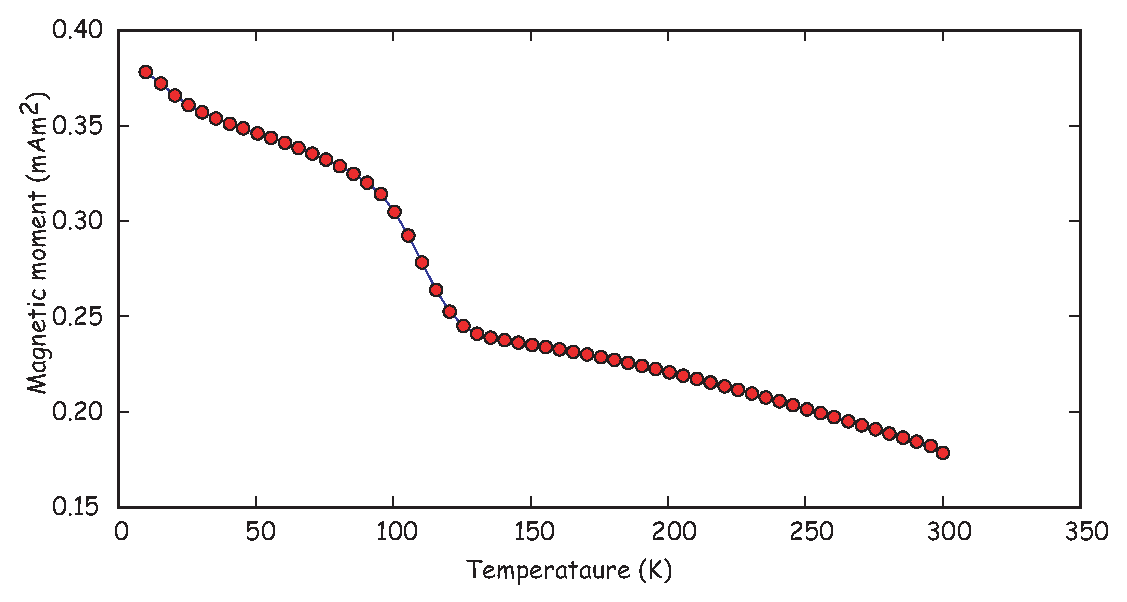
\includegraphics[width=12 cm]{EPSfiles/verwey.eps}
\caption{Magnetization curve for magnetite as a function of temperature.  The specimen was placed in a very large field, cooled to near absolute zero, then warmed up.  The magnetization was measured as it warmed.  When it goes through the Verwey transition ($\sim$110 K), a fraction of the magnetization is lost. Data downloaded from ``w5000'' in the  \href{http://www.irm.umn.edu/bestiary}{Rock magnetic Bestiary} collection at the Institute for Rock Magnetism.}
\label{fig:verwey}
\end{figure}



Because electronic interactions depend heavily on inter atomic spacing, 
\index{magnetic!anisotropy energy!magnetocrystalline}
magnetocrystalline anisotropy constants are a strong function of temperature (see Figure~\ref{fig:K-T}).    In magnetite, $K_1$ changes sign at a temperature known as the 
\index{isotropic point}
{\it isotropic point}.  At the isotropic point, there is no large magnetocrystalline anisotropy.  The large energy barriers that act to keep the magnetizations parallel to the body diagonal are gone and the spins can wander more freely through the crystal.  Below the isotropic point, the energy barriers rise again, but with a different topology in which the crystal axes are the energy minima and the body diagonals are the high energy states.    
 



At room temperature, electrons hop freely between the ferrous and ferric ions on the B lattice sites, so there is no order.  Below about 120 K, there is an ordered arrangement of the ferrous and ferric ions.  Because of the difference in size between the two, the lattice of the unit cell becomes slightly distorted  and becomes monoclinic instead of cubic.  This transition occurs at what is is known as the
\index{Verwey transition}
 {\it Verwey temperature} ($T_v$).   Although the isotropic point (measured magnetically) and the Verwey transition (measured electrically)  are separated in temperature by about 15$^{o}$, they are related phenomena (the ordering and electron hopping cause the change in $K_1$).   

The change in magnetocrystalline anisotropy at low temperature can have a profound effect on the magnetization.  In Figure~\ref{fig:verwey} we show a typical (de)magnetization curve for magnetite taken from the ``Rock magnetic bestiary'' web site maintained at  the Institute for Rock Magnetism: \url{http://irm.umn.edu/bestiary}.  There is a loss of magnetization at around 100 K.  This loss is the basis for 
\index{demagnetization!low-temperature}
{\it low-temperature demagnetization} (LTD).  However, some portion of the magnetization always remains after low temperature cycling (called the {\it low temperature memory}), so the general utility of LTD may be limited.



Cubic symmetry (as in the case of  magnetite) is just one of many types of crystal symmetries.    One other very important form is the uniaxial symmetry which can arise from crystal shape or structure.  The energy density for uniaxial magnetic anisotropy is:

\begin{equation}
\epsilon_a  = K_{u1} sin^2 \theta + K_{u2} \sin^4 \theta + ...
\label{eq:Ku}
\end{equation}

\noindent Here the magnetocrystalline constants have been designated $K_{u1}, K_{u2}$ to distinguish them from $K_1, K_2$ used before.  
In this equation, when the largest
\index{magnetic!anisotropy energy!uniaxial}
{\it uniaxial anisotropy constant},  $K_{_u1}$, is negative, the magnetization is constrained to lie perpendicular to the axis of symmetry.  When $K_{u1}>0$, the magnetization lies parallel to it. 

An example of a mineral dominated by uniaxial symmetry is hematite, a mineral with hexagonal crystal symmetry.  The magnetization of hematite is quite complicated, as we shall learn in Chapters 6 and 7, but one source is  magnetization is 
\index{spin-canting}
spin-canting (see Chapter 3) within the basal plane of the hexagonal crystal.  Within the basal plane, the anisotropy constant is very low and the magnetization wanders fairly freely.  However, the anisotropy energy away from the basal plane is strong, so the magnetization is constrained to lie within the basal plane.  


\subsection {Magnetostriction - stress anisotropy}

Exchange energy depends strongly on the details of the physical interaction between orbitals in neighboring atoms with respect to one another, hence  changing the positions of these atoms will affect that interaction.  Put another way, straining a crystal will alter its magnetic behavior.  Similarly, changes in the magnetization can change the shape of the crystal by altering the shapes of the orbitals.  This is the phenomenon of  
\index{magnetic!anisotropy energy!magnetostriction}
{\it magnetostriction}.    The magnetic energy density caused by the application of stress to a crystal be approximated  by:

$$
\epsilon_{\sigma} = {3\over 2} \bar \lambda \sigma \sin^2 \theta,
$$
\noindent where $\bar \lambda$ is an experimentally derived constant, $\sigma$ is the stress, and $\theta$ is the angle of the stress with with respect to the $c$ crystallographic axis.   Moskowitz (1993b)  \nocite{moskowitz93b} measured the magnetostriction constants parallel to [111] and [100] in magnetite and found $\lambda_{111}$ and  $\lambda_{100}$ to be 78.2x10$^{-6}$ and -21.8x10$^{-6}$  respectively.    $\bar \lambda$ is given by:

$$\bar \lambda = {2\over 5} \lambda_{100} + {3\over 5} \lambda_{111},
$$
so $\bar \lambda$  for magnetite is about 38 x 10$^{-6}$.   Stress has units of Nm$^{-2}$ which have the same fundamental units as Jm$^{-3}$, so $\bar \lambda$ is dimensionless.     Note the similarity in form of magnetostriction and uniaxial anisotropy giving rise to a single ``easy axis'' within the crystal. 


\begin{figure}[htb]
%\epsfxsize 14cm
%\centering \epsffile{EPSfiles/demagfield.eps}
\centering  \includegraphics[width=14 cm]{EPSfiles/demagfield.eps}
\caption{a) Internal magnetizations within a ferromagnetic crystal.  b) Generation of an identical external field from a series of surface monopoles.  c) The internal ``demagnetizing'' field resulting from the surface monopoles. [Redrawn from O'Reilly, 1984]. d) Surface monopoles on a sphere.  e) Surface monopoles on an ellipse, with the magnetization parallel to the elongation.  f) Demagnetizing field $\H_d$ resulting from magnetization $M$  at angle $\theta$ from $a$ axis in prolate ellipsoid.}
\label{fig:demagfield}
\end{figure}



\subsection {Magnetostatic (shape) anisotropy}
\label{sect:shape}

There is one more important source of 
\index{magnetic!anisotropy energy!shape}
magnetic anisotropy:  shape.    To understand how crystal shape controls magnetic energy, we need to understand the concept of the internal 
\index{demagnetizing!field (internal)}
{\it demagnetizing field}  of a magnetized body.   In Figure~\ref{fig:demagfield}a we show  the magnetic vectors within a ferromagnetic crystal.  These produce a magnetic field external to the crystal that is proportional to the magnetic moment (see Chapter 1).   This external field is identical to a field produced by a set of  {\it free poles} distributed over the surface of the crystal (Figure~\ref{fig:demagfield}b).    The surface poles do not just produce the external field, they also produce an internal field shown in Figure~\ref{fig:demagfield}c.  The internal field is known as the 
\index{demagnetizing!field}
{\it demagnetizing field} ($H_d$). $H_d$ is proportional to the magnetization of the body and is sensitive to the shape.   For a simple sphere in Figure~\ref{fig:demagfield}a and applied field condition shown in Figure~\ref{fig:demagfield}d, the demagnetizing field is given by:

$$
\H_d = -N \M,
$$

\noindent where $N$ is a
\index{demagnetizing!factor}
 {\it demagnetizing factor} determined by the shape.  In fact, the demagnetizing factor depends on the orientation of $\M$ within the crystal and therefore is a tensor (see Appendix~\ref{app:tensors} for review of tensors).  The more general equation is $\H_d = {\bf N} \cdot \M$ where $\H_d$ and $\M$ are vectors and $\bf N$ is a 3 x 3 tensor.  For now, we will simplify things by considering the isotropic case of a sphere in which ${\bf N}$ reduces to the single value scalar quantity $N$.  

 For a sphere,  the surface poles are distributed  over the surface such that there are none at the ``equator'' and most at the ``pole'' (see Figure~\ref{fig:demagfield}d).   Potential field theory shows that the external field of a uniformly magnetized body is identical to that of a centered dipole moment of magnitude $m=v M$ (where $v$ is volume).  At the equator of the sphere as elsewhere, $\H_d = -N\M$. But the  external field at the equator is equal to the demagnetizing field just inside the body because the field is continuous across the body.  We can find the equatorial (tangential) demagnetizing  field at the equator  by substituting in the equatorial colatitude $\theta=90^{\circ}$ into $H_{\theta}$ in  Equation~\ref{eq:HrHt} from Chapter 1), so:

$$
H_d   = -{m \over {4\pi r^3}}.
$$
\noindent   Using the fact that magnetization (in units of Am$^{-1}$) is the moment (in units of Am$^2$) per unit volume (in units of m$^3$) and the volume of a sphere is ${4\over 3} \pi r^3$, we have:

$$m={4\over 3} \pi r^3 M,
$$

\noindent
 so substituting and solving for $H_d$ we get $H_d=-{1\over 3} M$, hence $N={1\over 3}$.    

Different directions within a non-spherical crystal will have different distributions of free poles (see Figures~\ref{fig:demagfield}e,f).  In fact the surface density of free poles is given by $\sigma_m=\M\cdot \hat r$.  Because the surface pole density depends on the direction of magnetization, so too will  $N$.   In the case of a prolate ellipsoid magnetized parallel to the elongation axis $a$ (Figure~\ref{fig:demagfield}e), the free poles are farther apart than across the grain, hence, intuitively, the demagnetizing field, which depends on $1/r^2$, must be less than in the case of a sphere.  Thus, ${{N_a} < } {1\over 3}$.  Similarly, if  the ellipsoid is magnetized along $b$ (Figure~\ref{fig:demagfield}e), the demagnetizing field is stronger or $N_b>{1\over 3}$.     

Getting back to the magnetostatic energy density, $\epsilon_m = \M \cdot \B$,  remember that $\B$ includes both the external field $B_e = -\mu_o H_e$ and the internal demagnetizing field $\mu_o {\bf N}\cdot \M$.   Therefore, magnetostatic energy density from both the external and internal fields is given by:

\begin{equation}
\epsilon_{ms} = -\M \cdot  \mu_o  \H_e -{1\over 2} \mu_o \M \cdot {\bf N} \cdot \M. 
\label{eq:etot}
\end{equation}

\noindent  The two terms in Equation~\ref{eq:etot} are the by now familiar magnetostatic energy density $\epsilon_m$,  and the {\it magnetostatic self energy density} or the {\it demagnetizing energy density} $\epsilon_{d}$.  $\epsilon_d$  can be estimated by ``building'' a magnetic particle and considering the potential energy gained by each incremental volume $dv$ as it is brought in ($-\mu_o \M dv \cdot \H_d$) and integrating.  The $1\over 2$ appears in order to avoid counting each volume element   twice and the $v$ disappears because all the energies we have been discussing are energy densities -- the energy per unit volume.  


  For the case of a uniformly magnetized sphere, we get back to the relation $\H_d = -N\M$ and $\epsilon_d$ simplifies to:

\begin{equation}
\epsilon_d = -{1\over 2} \mu_o N M^2. 
\end{equation}

\noindent In the more general case of a prolate ellipsoid,  $\M$ can be represented by the two components parallel to the $a$ and $b$ axes (see Figure~\ref{fig:demagfield}f)  with unit vectors parallel to them $\hat a, \hat b$.  So,  $\M = M\cos \theta  \hat a + M\sin \theta \hat b$.   Each  component of $\M$ has an associated demagnetizing field $\H_d= -N_a M \cos  \theta \hat a - N_b M \sin \theta \hat b$ where $N_a, N_b$ are the eigenvalues of the tensor ${\bf N}$ (the values of  the 
\index{demagnetizing!tensor}
demagnetizing tensor along the principal axes $a$ and $b$).    In this case, the 
\index{demagnetizing!energy}
 demagnetizing energy can be written as: 

$$
\epsilon_d =-{1\over 2} \mu_o(N_a \cos^2 \theta + N_b \sin^2 \theta)M^2
 = -{1\over 2} \mu_o(N_a + (N_b-N_a)\sin^2 \theta)M^2
 $$
\begin{equation}
 = -{1\over 2} \mu_o(N_b\sin^2 \theta)M^2.
\label{eq:ed}
\end{equation}


In an ellipsoid with  three unequal axes $a,b,c$, $N_a+N_b+N_c =1$ (in SI; in cgs units  the sum is  4$\pi$).    For a  long needle-like particle, $N_a\simeq 0$ and ${N_b = N_c }\simeq {1\over 2}$.  
A useful approximation for nearly spherical particles is   $N_a = {1\over 3} [ 1 - {2\over 5}(2 - {b\over a} - {c\over a} )]$ 
\nocite{stacey74}
\index{Stacey, F.}
\index{Banerjee, S.K.}
(Stacey and Banerjee, 1974).     For more spheroids, see 
\nocite{nagata61}
\index{Nagata, T.}
Nagata (1961, p. 70)  and for the general case, see 
\index{Dunlop, D.J.}
\index{\"Ozdemir, \"O.}
\nocite{dunlop97}
Dunlop and \"Ozdemir (1997).   
In the absence of an external field, the magnetization will be parallel to the long axis ($\theta=0$) and the magnetostatic energy density (also known as the `self' energy is given by: 

\beq
\epsilon_{ms}= -{1\over 2} \mu_o N_c M^2.
\label{eq:self}
\eeq

\noindent  Note that the demagnetizing energy in Equation~\ref{eq:ed}  has a uniaxial form, directionally dependent only on $\theta$,  with the constant of uniaxial anisotropy $K_u = {1\over 2} \Delta N \mu_o M^2$. $\Delta N$ is the difference between the largest and smallest values of the demagnetizing tensor  $N_c-N_a$.  

For a prolate ellipsoid $N_c=N_b$ and  choosing for example  $c/a = 1.5$ we find that  $N_a-N_c = \sim 0.16$.   The magnetization of magnetite is 480 kAm$^{-1}$, so $K_u \simeq$ 2.7 x 10$^4$ Jm$^{-3}$.  This is somewhat larger than the absolute value of $K_1$  for magnetocrystalline anisotropy in magnetite ($K_1$= -1.35 x 10$^{4}$ Jm$^{-3}$), so the magnetization  for even slightly elongate grains will be dominated by uniaxial anistropy controlled by shape.     Minerals with low saturation magnetizations (like hematite) will not be prone to shape dominated magnetic anisotropy, however.

\begin{figure}[htb]
%\epsfxsize 12cm
%\centering \epsffile{EPSfiles/micromag.eps}
\centering  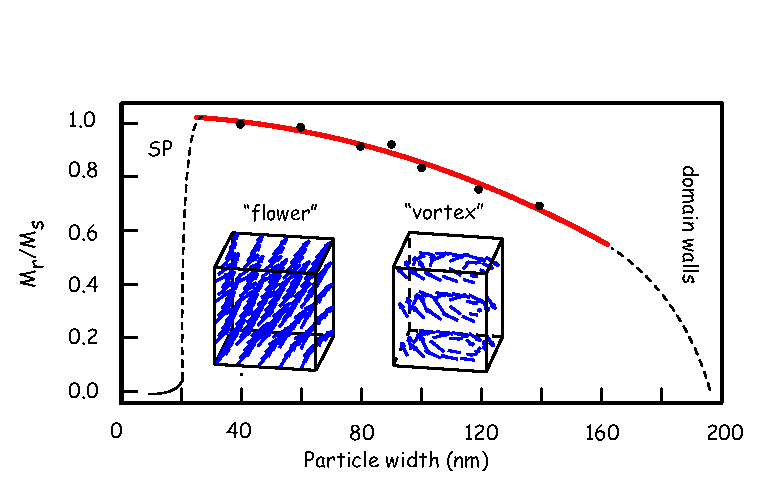
\includegraphics[width=12 cm]{EPSfiles/micromag.eps}
\caption{Possible non-uniform magnetization configurations that reduce self energy for magnetite with increasing particle widths.  The net remanent magnetization reduces with increasingly non-uniform spin configurations.    [Data from Tauxe et al., 2002.]}
\label{fig:nonuniform}
\end{figure}
\nocite{tauxe02}



\subsection{Magnetic energy and magnetic stability}
\label{sect:coercivity}

 Paleomagnetists worry about how long a magnetization can remain fixed within a particle and we will begin to discuss this issue later in the chapter.  It is worth pointing out here that any discussion of magnetic stability will involve magnetic anisotropy energy because this controls the energy required to change a magnetic moment from one easy axis to another.      One way to accomplish this change is to apply a magnetic field sufficiently large that its magnetic energy exceeds the  anisotropy energy.  The magnetic field  capable of flipping the magnetization of an individual uniformly magnetized particle (at saturation, or  $M_s$) over the magnetic anisotropy energy barrier  is the
 \index{coercivity!microscopic}
 \index{magnetic!anisotropy energy!cubic}
  {\it microscopic coercivity} $H_k$.  For uniaxial anisotropy ($K=K_u$) and for cubic magnetocrystalline  anisotropy ($K=K_1$), 
 microscopic coercivity is  given by:
 
\begin{equation}
 H_k = {{ 2 K_u}\over {\mu_oM}}   = { {4\over 3}}{ { |K_1|}\over {\mu_o M_s}}.  
\label{eq:Bk}
\end{equation}

\noindent  respectively (see
\index{Dunlop, D.J.}
\index{\"Ozdemir, \"O.}
\nocite{dunlop97}
Dunlop and \"Ozdemir, 1997 for a more complete derivation).   For elongate particles dominated by shape anisotropy,   $H_k$ reduces to  $  \Delta NM$.  [Note that the units for coercivity as derived here are in Am$^{-1}$, although they are often measured using instruments calibrated in tesla.   Technically,  because the field doing the flipping is inside the magnetic particle and $\B$ (measured in tesla) depends on the magnetization $\M$ as well as the field $\H$ (Equation~\ref{eq:B}), coercivity should be written as $\mu_o H_k$ if the units are quoted in tesla. Microscopic coercivity is another parameter with many names: 
\index{flipping!field}
\index{coercivity}
{\it flipping field}, {\it switching field}, {\it intrinsic coercivity} and also more loosely,   the  {\it coercive field} and {\it coercivity}. We will come back to the  topic of coercivity in Chapter 5.  ]


\begin{figure}[h!tb]
%\epsfxsize 14cm
%\centering \epsffile{EPSfiles/domains.eps}
\centering  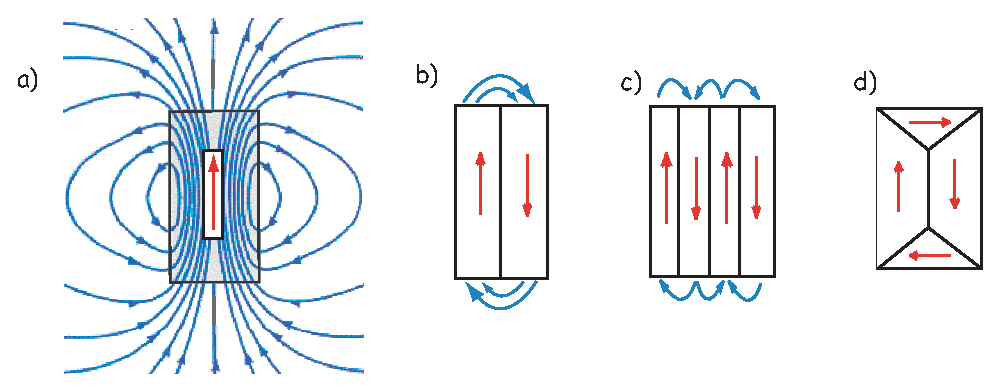
\includegraphics[width=14 cm]{EPSfiles/domains.eps}
\caption{A variety of domain structures of a given particle.  a) Uniformly magnetized (single domain).   [Adapted from Tipler, 1999.] b) Two domains.  c) Four domains in a lamellar pattern.  d) Essentially two domains with two closure domains.}
\label{fig:domains}
\end{figure}
\nocite{tipler99}



\section {Magnetic domains}


So far we have  been discussing hypothetical magnetic particles that are uniformly magnetized. Particles with strong magnetizations (like magnetite) have self energies that quickly become quite large because of the dependence on the square of the magnetization.   We have been learning about several mechanisms that tend to align magnetic spins. In fact in very small particles of magnetite ($<$ 40 nm), the  spins are essentially lined up.  The particle is uniformly magnetized  and we called it single domain (SD).  In larger particles  ($\sim$80 nm) the self energy exceeds the other exchange and magnetocrystalline energies and  crystals  have distinctly non-uniform states of magnetization.   


There are many strategies possible for magnetic particles to reduce self energy.    Numerical models (called {\it micromagnetic models}) can find internal magnetization configurations that minimize the energies discussed in the preceding sections.  
\index{micromagnetic modeling}
Micromagnetic simulations for magnetite particles 
\nocite{schabes88}
\index{Schabes, M.E.}
\index{Bertram, H.N.}
(e.g. Schabes and Bertram, 1988)  allow us to peer into the state of magnetization inside magnetic particles.  These simulations give a picture of increasing complexity from  so-called 
\index{flower remanent state}
\index{vortex remanent state}
{\it flower} to {\it vortex} (Figure~\ref{fig:nonuniform}) remanent states.  These particles share many properties of the uniformly magnetized single domain particles and are called 
\index{pseudo-single domain}
{\it pseudo-single domain} (PSD) particles.  




As particles grow larger ($>\sim$200 nm), they break into multiple 
\index{magnetic!domains}
magnetic domains,  separated by narrow zones of rapidly changing spin directions called
\index{magnetic!domain walls}
 {\it domain walls}.   Magnetic domains can take many forms.  We illustrate a few in Figure~\ref{fig:domains}. The uniform case (single domain) is shown in  Figure~\ref{fig:domains}a.  The external field is very large because the free poles are far apart (at opposite ends of the particle).   When the particle organizes itself into two domains (Figure~\ref{fig:domains}b), the external field is reduced by about a factor of two.  In the case of four lamellar domains (Figure~\ref{fig:domains}c), the external field is quite small.  The introduction of {\it closure domains} as in Figure~\ref{fig:domains}d reduces the external field to nothing.  

\begin{figure}[htb]
%\epsfxsize 14.5cm
%\centering \epsffile{EPSfiles/wall.eps}
\centering  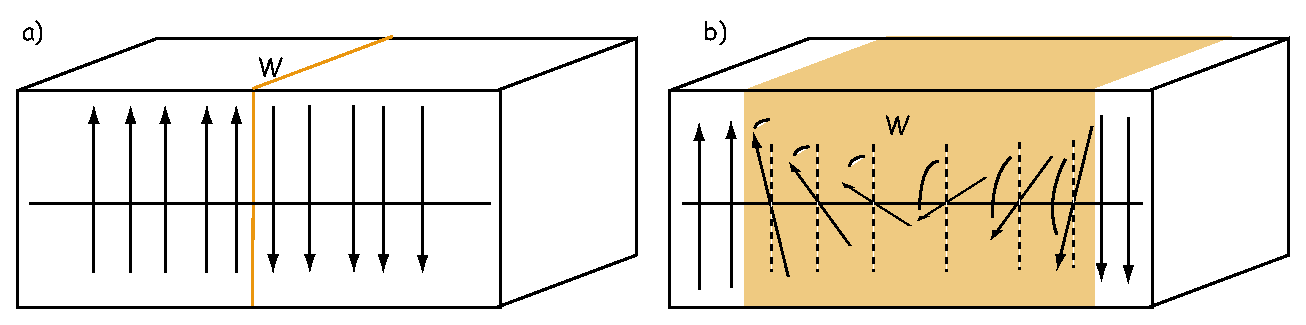
\includegraphics[width=14.5 cm]{EPSfiles/wall.eps}
\caption{Examples of possible domain walls.  a) There is a 180$^{\circ}$ switch from one atom to the next.  The domain wall is very thin, but the exchange price is very high.  b) There is a more gradual switch from one direction to the other [note: each arrow represents several 10's of unit cells].  The exchange energy price is lower, but there are more spins in unfavorable directions from a magnetocrystalline point of view.  }
\label{fig:wall}
\end{figure}
%\eject



As you might already suspect, domain walls are not  ``free'', energetically speaking.  If, as in Figure~\ref{fig:wall}a, the spins simply switch from one orientation to the other abruptly,  the exchange energy cost would be very high.  One way to get around this  to spread the change over several hundred atoms, as sketched in Figure~\ref{fig:wall}b.  The wall width $\delta$ is wider and the exchange energy price is much less.  However, there are now spins in unfavorable directions from a magnetocrystalline point of view (they are in ``hard'' directions).   Exchange energy therefore favors wider domain walls while magnetocrystalline anisotropy favors thin walls.    With some work (see e.g.,  \index{Dunlop, D.J.}
\index{\"Ozdemir, \"O.}
\nocite{dunlop97}
Dunlop and \"Ozdemir, 1997, pp. 117-118), it is possible to come up with the following analytical expressions for wall width ($\delta_w$) and 
\index{magnetic!domain walls!energy}
wall energy density  ($\epsilon_w$):

\beq
\delta_w = \pi {\bigl( {A\over K} \bigr)}^{1\over 2},  \epsilon_w = 2\pi (AK)^{1\over 2},
\label{eq:wall}
\eeq
\noindent where $A$ is the 
\index{magnetic!energy!exchange!constant}
exchange constant  (see Section~\ref{sect:exchange}) and $K$ is the magnetic anisotropy constant (e.g., $K_u$ or $K_1$).   Note that $\epsilon_w$ is the energy density per unit wall area, not per volume.    Plugging in values for magnetite given previously we get $\delta_w$ = 90 nm and $\epsilon_w$  = 3x 10$^{-3}$Jm$^{-2}$.    



In Figure~\ref{fig:energies} we plot the 
\index{magnetic!self energy}
self energy (Equation~\ref{eq:self})  and the wall energy ($\epsilon_w$ from Equation~\ref{eq:wall}) for spheres of magnetite.  We see that the wall energy in  particles with diameters of some 50 nm  is less than the self energy, yet the width of the walls about twice as wide as that.  So the smallest wall is really more like the vortex state and it is only for particles larger than a few tenths of a micron that true domains separated by discrete walls can form.   Interestingly, this is precisely what is predicted from micromagnetic modelling (e.g., Figure~\ref{fig:nonuniform}).   


\begin{figure}[htb]
%\epsfxsize 9.5cm
%\centering \epsffile{EPSfiles/energies.eps}
\centering  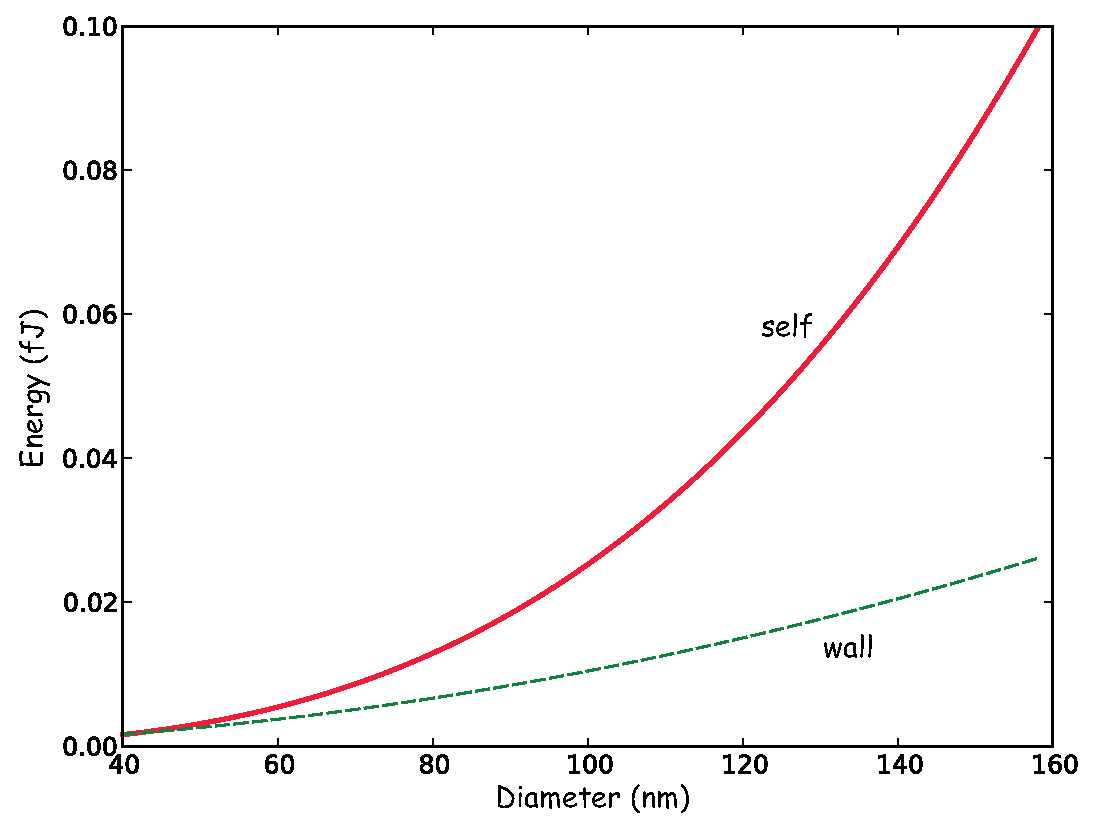
\includegraphics[width=9.5 cm]{EPSfiles/energies.eps}
\caption{Comparison of ``self'' energy versus the energy of the domain wall in magnetite spheres as a function of particle size.}
\label{fig:energies}
\end{figure}



How can we test the theoretical predictions of domain theory?  Do domains really exist?  Are they the size and shape we expect?  Are there as many as we would expect?    In order to address these questions we require a way  of imaging magnetic domains.  
\index{Bitter, F.}
Bitter (1931) \nocite{bitter31} devised a way for doing just that.  Magnetic domain walls are regions with large stray fields (as opposed to domains in which the spins are usually parallel to the sides of the crystals to minimize stray fields).  In the
\index{domain imaging!Bitter technique}
 {\it Bitter technique} magnetic colloid material is drawn to the regions of high field gradients on highly polished sections  allowing the domain walls to be observed (see Figure~\ref{fig:domain-images}a).  

\begin{figure}[h!tb]  
%\epsfxsize 11cm
%\centering \epsffile{EPSfiles/domain-images.eps}
\centering  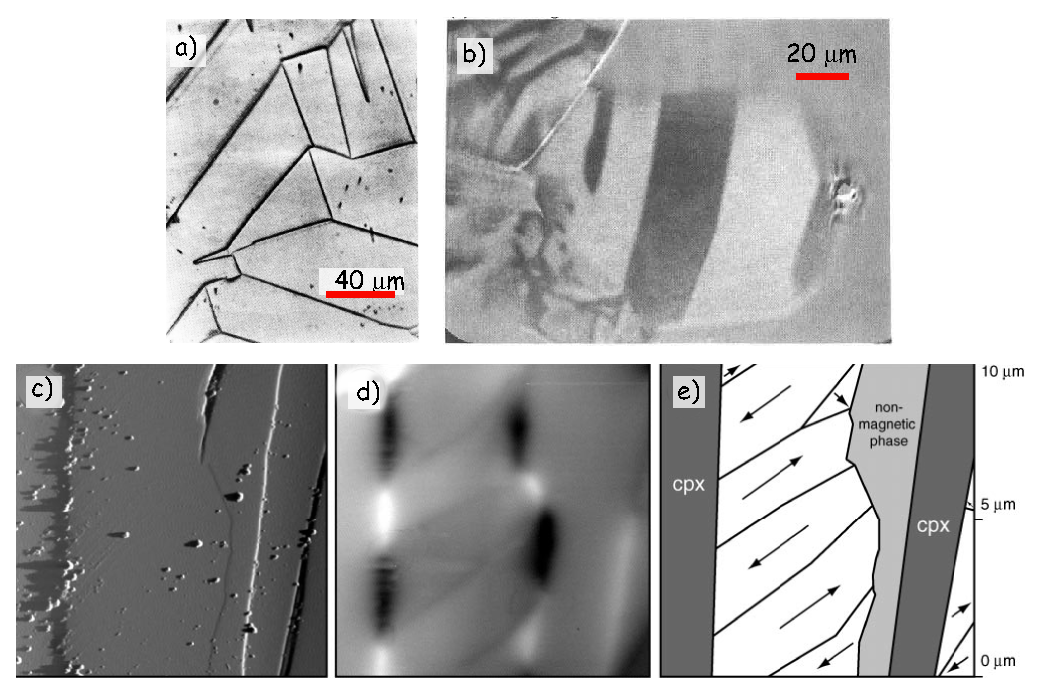
\includegraphics[width=11 cm]{EPSfiles/domain-images.eps}
\caption{a) Bitter patterns from an oriented polished section of magnetite. [Figure from \"Ozdemir et al., 1995]. b) Domains revealed by longitudinal magneto-optical Kerr effect. [Image from Heider and Hoffmann, 1992.]  c-e)  Magnetic force microscopy technique. [Images from Feinberg et al., 2005.] c) Image of topography of surface of a magnetite inclusion in a non-magnetic matrix.  d) Magnetic image from MFM techqnique.  e) Interpretation of magnetizations of magnetic domains.   }
\label{fig:domain-images}
\end{figure}
\nocite{feinberg05}  \nocite{heider92} \nocite{ozdemir95}

There are by now other ways of imaging magnetic domains.  We will not review them all here, but will just highlight the ways that are more commonly used in rock and paleomagnetism.  The
\index{domain imaging!magneto-optical Kerr effect} 
{\it magneto-optical Kerr effect}  or MOKE  uses the interaction between polarized light and the surface magnetic field of the target.   The light interacts with the magnetic field of the sample which causes a small change in the light's polarization and ellipticity.   The changes are detected by reflecting the light into nearly-crossed polarizers.   The longitudinal Kerr effect can show the alignment of magnetic moments in the surface plane of the sample. Domains with different magnetization directions show up as lighter or darker regions in the MOKE image (see Figure~\ref{fig:domain-images}b.) 


Another common method for imaging magnetic domains employs a technique known as 
\index{domain imaging!magnetic  force microscopy}
{\it magnetic force microscopy}.  
Magnetic force microscopy (MFM) uses a scanning probe microscope that maps out the vertical component of the magnetic fields produced by a highly polished section.   The measurements are made with a cantilevered magnetic tip that responds to the magnetic field of the sample.  In practice, the measurements are made in two passes.  The first establishes the topography of the sample (Figure~\ref{fig:domain-images}c).  Then in the second pass, the tip is raised slightly above the surface and by subtracting the �topographic only� signal the attraction of the magnetic surface can be mapped (Figure~\ref{fig:domain-images}d).   Figure~\ref{fig:domain-images}e shows an interpretation of the magnetic directions of different magnetic domains.  



\section{Thermal energy}
\label{sect:tau}

\index{thermal energy}
We have gone some way toward answering the questions posed at the beginning of the chapter. We see now that  anisotropy energy, with contributions from crystal structure, shape and stress, that inhibits changes in the magnetic direction thereby offering a possible mechanism whereby a given  magnetization could be preserved for posterity.  We also asked the question of what allows the magnetization to come into equilibrium with the applied magnetic field in the first place;  this question requires a little more work to answer.  The key to this question is to find some mechanism which allows the moments to ``jump over'' magnetic anisotropy energy barriers.   One such mechanism is  thermal energy $E_T$, which was given in Chapter 3 as:

$$
E_T = kT.
$$

We know from statistical mechanics that the probability $P$ of finding a grain with a given thermal energy  sufficient to overcome some anisotropy energy $E_a$ and change from one easy axis to another is $P=\exp (-E_a/E_T )$.   Depending on the temperature,  such grains may be quite rare, and we may have to wait some time $t$ for a particle to work itself up to jumping  over the energy barrier.  


\begin{figure}[htb]
%\epsfxsize 10cm
%\centering \epsffile{EPSfiles/tauvd.eps}
\centering  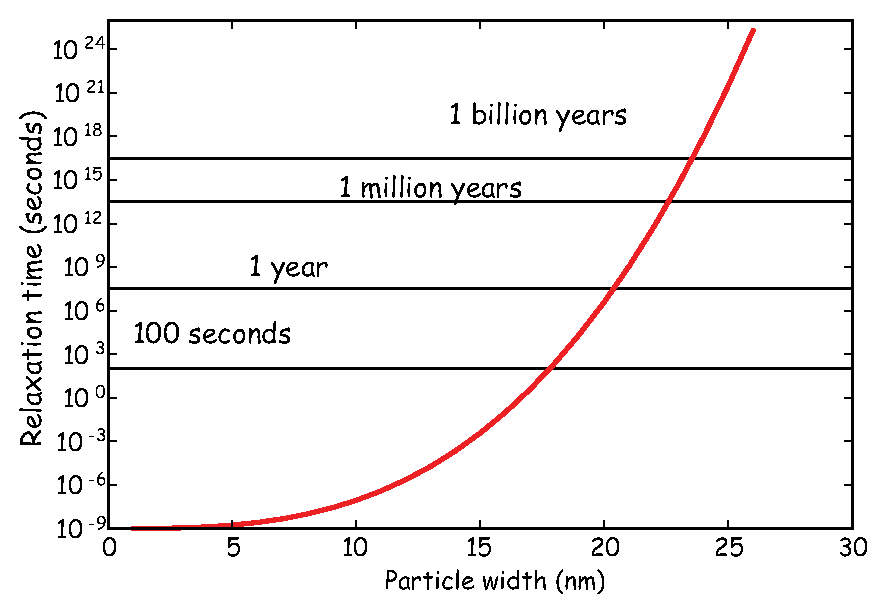
\includegraphics[width=9.5 cm]{EPSfiles/tauvd.eps}
\caption{Relaxation time in magnetite ellipsoids as a function of grain width in nanometers (all length to width ratios of 1.3:1.)  }
\label{fig:tauvd}
\end{figure}
 


Imagine a block of material containing a random assemblage of magnetic particles that are for simplicity uniformly magnetized  and dominated by uniaxial anisotropy.  Suppose that this block has some initial magnetization $M_o$ and is placed in an environment with no ambient magnetic field.  Anisotropy energy will tend to keep each tiny magnetic moment in its original direction and the magnetization will not change over time.  At some temperature,  certain grains will have sufficient energy to overcome the anisotropy energy and flip their moments to the other easy axis.   As the energy surface is spherical, with no dimples or protruberances, there is no preferred direction and, over time, the magnetic moments will become random.  
Therefore, the magnetization as a function of time in this simple scenario will decay to zero.  The equation governing this decay is:  

\begin{equation}
M(t) = M_o \exp ({-t\over {\tau}}),
\label{eq:MvT}
\end{equation}

\noindent where $t$ is time and $\tau$ is an empirical constant called the {\it relaxation time}.  Relaxation time is   the time required for the remanence to decay to $1/e$ of $M_o$.    This equation is the essence of what is called
\index{N\'eel!theory}
\index{N\'eel, L.}
{\it N\'eel theory}
  \nocite{neel55} 
  (see, e.g., N\'eel, 1955).
\index{relaxation time}
The value of $\tau $ depends on the  competition between 
magnetic anisotropy energy and 
thermal energy.  It is a measure of the probability that a grain will have
sufficient thermal energy to overcome the anisotropy energy and switch its
moment.  Therefore in zero external field:

\begin{equation}
{\tau } = {{1\over C} \exp
{[{\hbox{anisotropy}\hskip 1em \hbox{energy}}]\over
[{\hbox{thermal }\hskip 1em \hbox{energy}}]}} =
{{1\over C} \exp {[K v]\over [kT]}},
\label{eq:tau}
\end{equation}

\noindent where $C$ is a 
frequency factor with a value of something like
$10^{10}$ s$^{-1}$.  The anisotropy energy is given by the dominant 
anisotropy parameter $K$ (either $K_u, K_1$, or $\lambda$)
 times the grain volume $v$.  
 
\index{thermal energy}%

Thus,  the 
\index{relaxation time}%
relaxation time is proportional to anisotropy constant and 
volume, and is inversely related to
temperature.
\index{relaxation time}%
Relaxation time $\tau $ varies  rapidly with small changes in $v$ and $T$.
To see how this works, we can take $K_u$ for slightly elongate cuboids of  magnetite (length to width ratio of 1.3 to 1)  and evaluate relaxation time as a function of particle width (see Figure~\ref{fig:tauvd}).   There is a sharp transition between grains with virtually no stability
($\tau $ is on the order of seconds) and grains with stabilities of billions of years. 

Grains with $\tau \simeq 10^2 - 10^3$ seconds have sufficient thermal energy
to overcome the anisotropy energy frequently and are unstable on a laboratory
time scale.  In zero field, these grain moments will tend to rapidly
become random,  and
in an applied field, also tend to align  rapidly with the field.  
The net magnetization is related to the field by a
Langevin function (see Section~\ref{sect:para} in Chapter 3).  Therefore, this
 behavior is quite similar to paramagnetism, hence these grains are called 
\index{superparamagnetism}%
{\it superparamagnetic} (SP). Such grains can be distinguished from paramagnets,
however, because the field required to saturate the moments is typically much
less than a tesla, whereas that for paramagnets can exceed hundreds of
tesla. 

\begin{figure}[h!tb]
%\epsfxsize 9.5cm
%\centering \epsffile{EPSfiles/butban.eps}
\centering  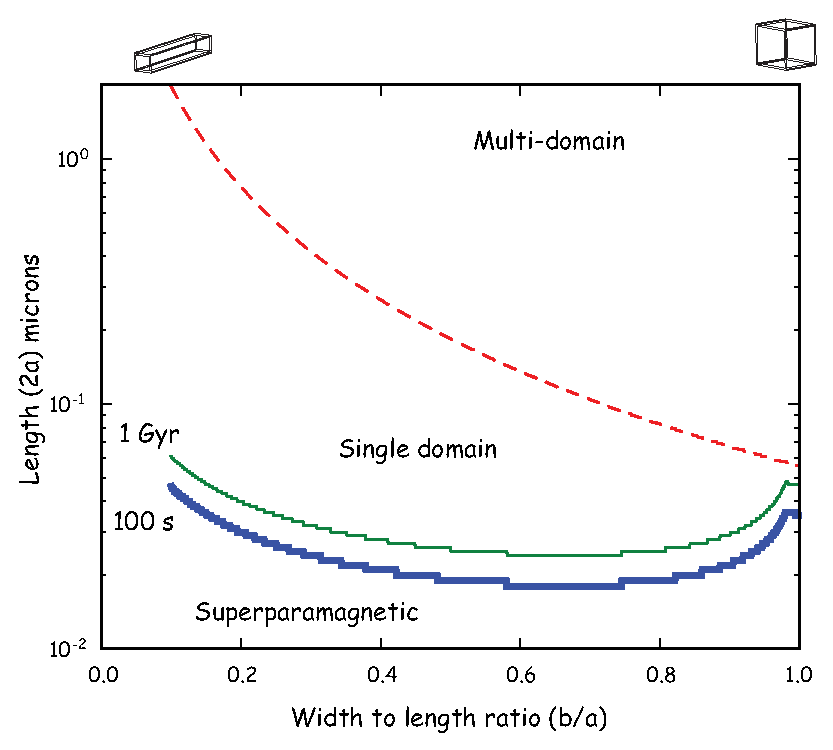
\includegraphics[width=9.5 cm]{EPSfiles/butban.eps}
\caption{ Expected domain states for various sizes and shapes of  parallelopipeds of magnetite at room temperature.  The parameters $a$ and $b$ are as in Figure 4.4e.  Heavy blue (thin green) line is the superparamagnetic threshold assuming a relaxation time of 100s (1 Gyr).   Dashed red line marks the SD/MD threshold size.  Calculations done using assumptions and parameters described in the text.  }
\label{fig:butban}
\end{figure}


\section{Putting it all together}


We are now in a position to pull together all the threads we have considered in this chapter and make a plot of what sort of magnetic particles behave as superparamagnets, which should be single domain and which should be multi-domain according to our simple theories.   We can estimate the superparamagnetic to single domain threshold for magnetite as a function of particle shape by finding for the length (2a) that gives a relaxation time of 100 seconds as a function of width to length ratio ($b/a$) for parallelopipeds of magnetite (heavy blue line in  Figure~\ref{fig:butban}).    To do this, we  follow the logic of  
\index{Evans, M.E.}
\index{McElhinny, M.W.}
Evans and McElhinny (1969) \nocite{evans69} and 
\nocite{butler75}  
\index{Butler, R.F.}
\index{Banerjee, S.K.}
 Butler and Banerjee (1975).   In this 
\index{diagrams!Evans}
{\it Evans diagram}, we estimated relaxation time using  Equation~\ref{eq:tau},  plugging in  values of $K$ as either the magnetocrystalline effective anisotropy constant (${1\over{12}}K_1$) or the shape anisotropy constant (${1\over 2} \Delta N \mu_o M^2$), whichever was less.   We also show the curve at which relaxation time is equal to 1 Gyr, reinforcing the point that very small changes in crystal size and shape make profound differences in relaxation time.     
The figure also predicts the boundary between the single domain field and the two domain field,  when the energy of a domain wall is less than the self energy of a particle that is uniformly magnetized.  This can be done by evaluating wall energy with Equation~\ref{eq:wall} for a wall along the length of a parallelopiped and area ($4ab$) as compared to the self energy (${1\over 2} \mu_o N_a M^2v$) for a given length and width to length ratio.  When the wall energy is less than the self energy, we  are in the two domain field.    




Figure~\ref{fig:butban} suggests that there is virtually no SD stability field for equant magnetite; particles are either SP or MD (multi-domain).  As the width to length decreases (the particle gets longer), the stability field for SD magnetite expands.  Of course micromagnetic modelling shows that there are several transitional states between uniform magnetization (SD) and MD, i.e. the flower and vortex remaent states (see 
\nocite{fabian96} 
\index{Fabian, K.L.}
Fabian et al., 1996), but Figure~\ref{fig:butban} has  enormous predictive power and the version of 
\nocite{butler75}  
\index{Butler, R.F.}
\index{Banerjee, S.K.}
Butler and Banerjee (1975), (which is slightly different in detail)  continues to be used extensively.    It is worth pointing out however, that the size at which domain walls appear in magnetite is poorly constrained because it depends critically on the exact shape of the particle,  its state of stress and even its history of exposure to past fields.  Estimates in the literature range from as small as 20 nm  to much larger (up to 100 nm) depending on how the estimates are made.   Nonetheless, it is probably true that truly single domain magnetite is quite rare in nature, yet more complicated states are difficult to treat theoretically.   Therefore most paleomagnetic studies rely on predictions made for single domain particles.


\noindent{SUPPLEMENTAL READING:} Dunlop and \"Ozdemir (1997), Chapters 2.8 and 5.



\section{Problems}

{\parindent 0pt \parskip 12pt 

{\bf Problem 1}

Assume that the magnetization of magnetite is about 480 mAm$^{-1}$ and using values for other parameters from the text,  write a Python program to calculate  the following:

a) Self energy (or magnetostatic energy) for a sphere 1, 10 and 100 $\mu$m in diameter. [Hint: see Equation~\ref{eq:self}  in the text for the `self' energy density. Also, remember the difference between energy and energy density!] 

b) Magnetostatic (shape) anisotropy energy for an ellipsoid whose principal semi-axis is 1 $\mu$m and whose major and minor semi-axes are each 0.25 $\mu$m.  You may use the ``nearly spherical'' approximation in the text.   

c) The critical radius of a sphere at which wall energy equals self energy.


{\bf Problem 2}

Calculate  grain diameter for magnetite spheres with $\tau$s of 10$^{-1}$, 10, 10$^2$, 10$^3$, 10$^5$, 10$^9$, 10$^{15}$ seconds.  Use values for Boltzmann's constant, $C$ (the frequency factor) and $|K_1|$ at room temperature (300K).    

{\bf Problem 3}

Consider a highly elongate rod (needle-shaped grain) of ferromagnetic material.

a) Explain why the demagnetizing factor along the long axis of the rod is about zero and about one half across the axis.

b)  For a needle shaped grain of magnetite ($M_s=4.8\cross 10^5$ Am$^{-1}$), what external magnetic field is required to magnetize the rod to saturation along the diameter (perpendicular to the long axis)?

c) What is the maximum microscopic coercivity of magnetite (assume an infinitely long grain)?  
}



%http://www-physique.u-strasbg.fr/~udp/articles/chimie/weblab.htm

%http://www.ontariominerals.com/magnetite.htm

%http://www.gly.uga.edu/schroeder/geol3010/magnetite.gif

%http://www.geo.umn.edu/orgs/irm/bestiary/index.html

 % DONE 7/19/18
%\customlink{Magnetic_hysteresis}
\chapter {Magnetic hysteresis}




In Chapter  4 we discussed the energies  that control the state of magnetization within ferromagnetic particles.    Particles will tend to find a configuration of internal magnetization directions that minimizes the energies (although meta-stable states with 
\index{local energy minima}
{\it local energy minima} or LEMs are a possibility).    The longevity of a particular magnetization state has to do with the depth of the energy well that the magnetization is in and the energy available for hopping over barriers.  

The ease with which particles can be coerced  into changing their magnetizations in response to external fields can tell us much about the overall stability of the particles and perhaps also something about their ability to carry a magnetic remanence over the long haul.   The concepts of long term stability, incorporated into the concept of relaxation time and the response of  the magnetic particles  to external magnetic fields are therefore linked through the anisotropy energy constant $K$ (see Chapter  4) which  dictates the magnetic response of particles to changes in the external field.   This chapter will focus on  the response of magnetic particles to changing external magnetic fields.  



\section{The ``flipping'' field}
\label{sect:flipping}

Magnetic remanence is the magnetization in the absence of an external magnetic field.   If we imagine a particle with a single ``easy'' axis --  a so-called ``uniaxial'' particle with magnetic anisotropy constant $K_u$, the  magnetic energy density (energy per unit volume) of a particle whose magnetic moment makes an angle $\theta$ to the easy axis direction (Figure~\ref{fig:mB}a)  can be expressed as: 

$$
\epsilon_a = K_u\sin^2\theta.
$$


\noindent  As the moment swings around with angle $\theta$ to the easy axis, the anisotropy energy density $\epsilon_a$ will change as sketched in Figure~\ref{fig:mB}b.  The energy minima are when $\theta$ is aligned parallel to  the easy axis (an axis means either direction along the axis, so we pick one direction as being  0 and the other as 180$^{\circ}$).  In the absence of a magnetic field, the moment will lie along one of these two directions.  [In reality, thermal energy will perturb this direction somewhat, depending on the balance of anisotropy to thermal energy, but for the present discussion, we are assuming that thermal energy can be neglected.]  

\begin{figure}[h!tb]
%\epsfxsize 14cm
%\centering \epsffile{EPSfiles/mB.eps}
\centering  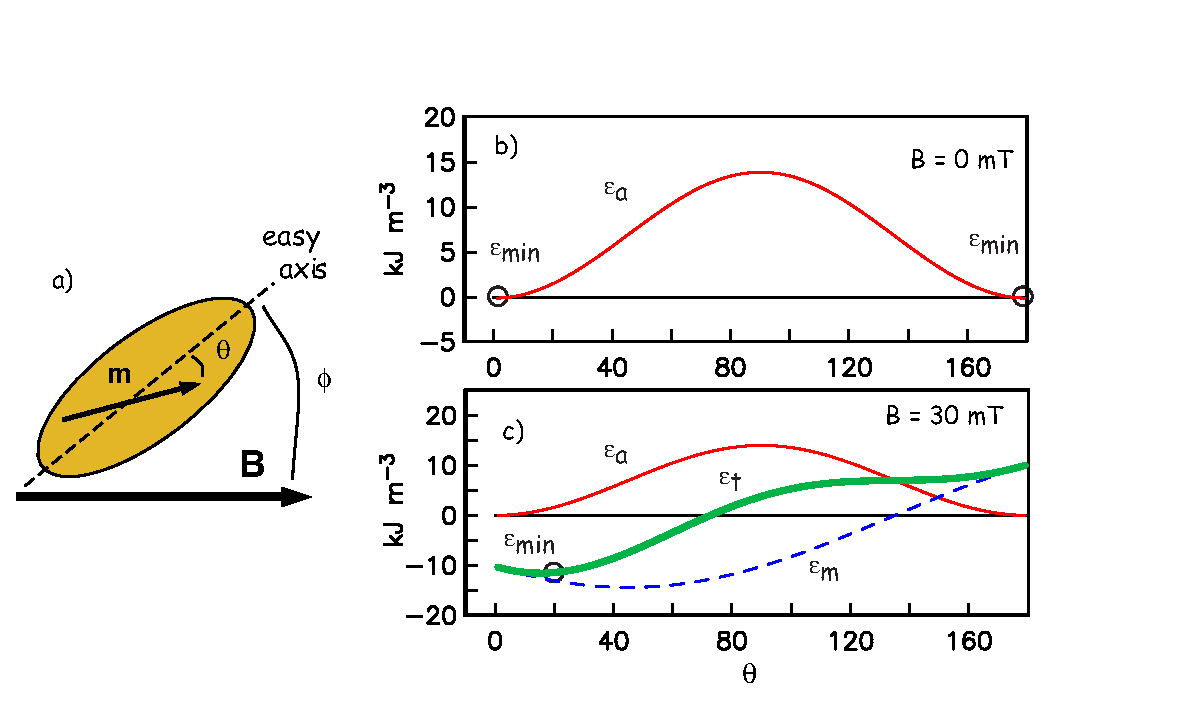
\includegraphics[width=14 cm]{EPSfiles/mB.eps}
\caption{a) Sketch of a magnetic particle with easy axis as shown.  In
response to a magnetic field $\B$, applied at an angle $\phi$ to the easy axis, the
particle moment $\m$ rotates, making an angle
$\theta$ with the easy axis. b) Variation of the anisotropy energy density  $\epsilon_a = K_u\sin^2\theta$ as a function of $\theta$ for the particle with $\phi=45^{\circ}$ as  shown in a). The $\theta$ associated with the minimum energy is indicated by $\epsilon_{min}$.  $B$ = 0 mT.  c) same as in b)  but for $B$ = 30 mT.  Also shown  the interaction energy density  $\epsilon_m=-M_s B\cos (\phi-\theta)$ and the total energy density $\epsilon_t=\epsilon_a+\epsilon_m$.}
\label{fig:mB}
\end{figure}



When an external field is applied at an angle $\phi$ to the easy axis (and an angle $\phi-\theta$ with the magnetic moment; see Figure~\ref{fig:mB}a), the magnetostatic  interaction energy  density $\epsilon_m$  given by the dot product of the magnetization and the applied field (Equation~\ref{eq:Em1}  in Chapter 4) or: 

  $$
\epsilon_m = -\M \cdot \B = -MB \cos(\phi-\theta).
 $$
 
 \noindent
The two energy densities  ($\epsilon_a$ and $\epsilon_m$) are shown as the thin solid and dashed lines  in Figure~\ref{fig:mB}c for an applied field of 30 mT aligned with an angle of 45$^{\circ}$ to the easy axis.   
There is a 
 competition between the anisotropy energy (tending to keep the magnetization parallel to the easy axis) and the interaction energy (tending to line the magnetization up with the external magnetic field).   Assuming that the magnetization is at saturation, we get the total energy density of the particle to be: 

 
\begin{equation}
\epsilon_t = K_u\sin^2\theta - M_s B \cos (\phi-\theta).
\label{eq:Et}
\end{equation}

\noindent  The total energy density $\epsilon_t$ is shown as the heavy solid line in Figure~\ref{fig:mB}c. 



The magnetic moment of a uniaxial single domain grain will find the angle $\theta$ that is associated with the minimum total energy density ($\epsilon_{min}$; see Figure~\ref{fig:mB}b,c).  For low external fields, $\theta$ will be closer to the easy axis  and for higher external fields (e.g., 30 mT; Figure~\ref{fig:mB}c), $\theta$ will be closer to the applied field direction ($\phi$).  



\begin{figure}[h!tb]
%\epsfxsize 14cm
%\centering \epsffile{EPSfiles/flip.eps}
\centering  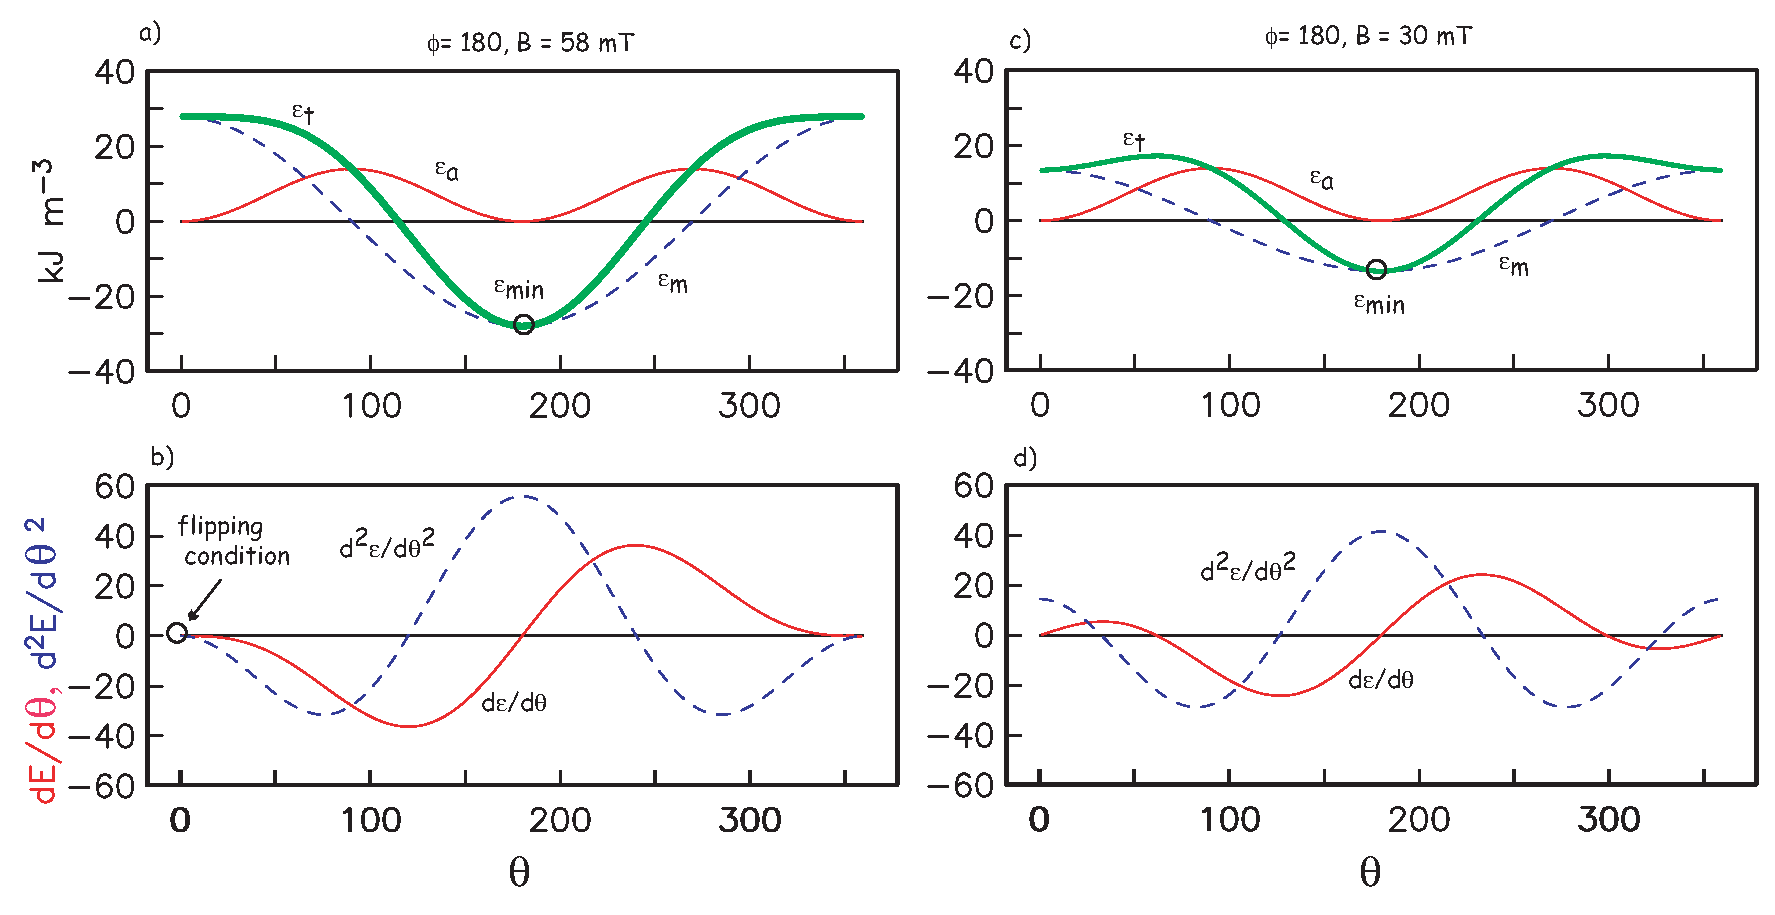
\includegraphics[width=14 cm]{EPSfiles/flip.eps}
\caption{a) Variation of the anisotropy energy density  $\epsilon_a = K_u\sin^2\theta$, the interaction energy density $\epsilon_m=-M_s B\cos \phi$ and the total energy density $\epsilon_t=\epsilon_a+\epsilon_m$ as a function of $\theta$ for the particle shown in Figure 5.1a.  The  field was applied with $\phi$ = 180$^{\circ}$ and was 58 mT in magnitude.  The $\theta$ associated with the minimum energy is indicated by $\epsilon_{min}$ and is 180$^{\circ}$.  b) Variation in first and second derivatives of the energy equation.  The flipping condition of both being zero simulaneously is met.  c) Same as a) but the field was only 30 mT.  d) Same as b but the flipping condition is not met.} 
\label{fig:flip}
\end{figure}


When a  magnetic field  that is large enough to overcome the anisotropy energy is applied in a direction opposite to the magnetization vector, the moment will jump over the energy barrier and stay in the opposite direction when the field is switched off.  The field necessary to accomplish this feat is called the 
\index{flipping!field}
\index{switching field}
{\it flipping field}  ($\mu_oH_f$)  (also sometimes the ``switching field'').    [Note the change to the use of $H$ for internal fields where $M$ cannot be considered  zero.)   \nocite{stoner48}   We introduced this parameter in Chapter 4 (see Equation~\ref{eq:Bk}) as the microscopic coercivity.   
\index{Stoner, C.}
\index{Wohlfarth, W.P.}
Stoner and Wohlfarth (1948)  showed that the flipping field can be found from the condition that $d\epsilon_t/d\theta = 0$ and $d^2\epsilon_t/d\theta^2$ = 0.  We will call this the 
\index{flipping!condition}
``flipping condition''.   The necessary equations can be found by differentiating Equation~\ref{eq:Et}:

\begin{equation}
{d\epsilon \over {d\theta}} = 2 K_u \sin \theta \cos \theta - M_s B \sin (\phi - \theta),
\label{eq:1stderiv}
\end{equation}
\noindent
and again

\begin{equation}
{d^2 \epsilon\over {d\theta^2}} = 2 K_u \cos (2\theta) + M_s B \cos (\phi - \theta ).
\label{eq:2ndderiv}
\end{equation}

\noindent Solving these two equations for $B$ and substituting $\mu_oH$ for $B$,  we get after some trigonometric trickery:

\begin{equation}
\mu_o H_f = { {2K_u \over {M_s} } 
{  {(1-t^2 + t^4)^{1\over 2} } \over {1 + t^2} } }=   {2K_u \over {M_s} }
{ 1 \over { (\cos ^{2\over 3}  \phi + \sin ^{2\over 3} \phi)^{3\over 2} }},
\label{eq:Bf}
\end{equation}

\noindent where $t= \tan^{1\over 3} \phi$.  In this equation, $\phi$ is the angle between the applied field and the easy axis direction opposite to $m$.    

Now we can derive  the so-called 
\index{coercivity!microscopic}
 ``microscopic coercivity'' ($H_k$)  introduced in  Section~\ref{sect:coercivity} in Chapter 4.  Microscopic coercivity is the maximum flipping field for a particle.    When  magnetic anisotropy  of a  particle is dominated by uniaxial anisotropy constant $K_u$ and $\phi$ is zero (antiparallel to the easy direction nearest the moment),   $\mu_o H_k = 2{ {K_u}\over {M_s} }$.     
Using the values appropriate for magnetite ($K_u$ = 1.4 x 10$^4$ Jm$^{-3}$ and $M_s$ = 480 mAm$^{-1}$ we get $\mu_o H_k$ = 58 mT.  To see why this would indeed result in a flipped moment, we plot the behavior of Equations~\ref{eq:Et} - \ref{eq:2ndderiv} in Figure~\ref{fig:flip}.  The minimum in total energy $\epsilon_t$ occurs at an angle of $\theta$ = 180$^{\circ}$ (Figure~\ref{fig:flip}a) and the first and second derivatives satisfy the flipping condition by having a common zero crossing ($\theta=0$ in Figure~\ref{fig:flip}b).   There is no other applied field value for which this is true (see, e.g., the case of  a 30 mT field in Figure~\ref{fig:flip}c,d). 

\begin{figure}[h!tb]
%\epsfxsize 7cm
%\centering \epsffile{EPSfiles/bf.eps}
\centering  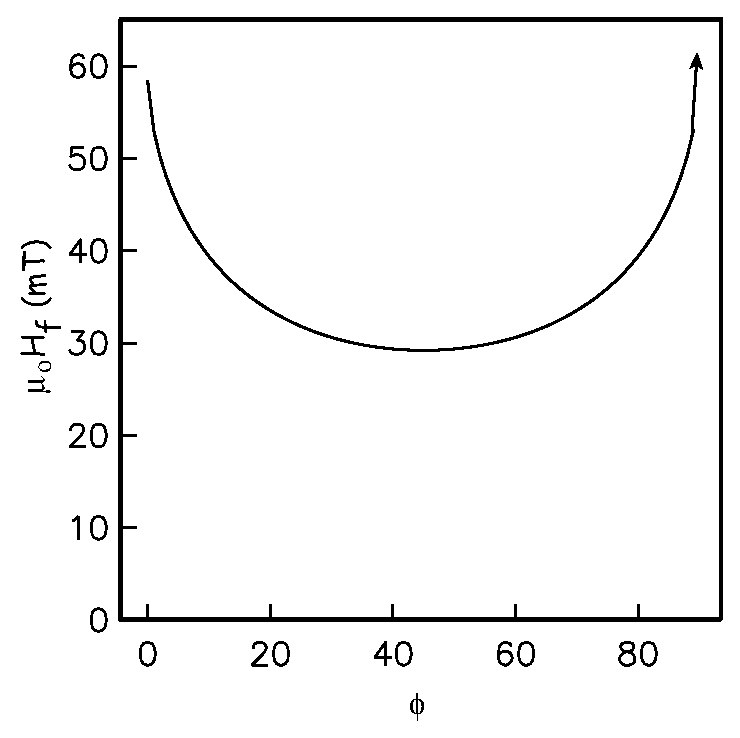
\includegraphics[width=7 cm]{EPSfiles/bf.eps}
\caption{The flipping field $\mu_oH_f$ required to irreversibly switch the magnetization vector from one easy direction to the other in a single domain particle dominated by uniaxial anisotropy. Note that $\phi$ is the angle with the easy axis, but must be the opposite direction from $\textbf{m}$.   }
\label{fig:bf}
\end{figure}


The flipping condition depends not only on the applied field magnitude but also on  the direction that it makes with the easy axis   (see $\mu_oH_f$ versus $\phi$ in Figure~\ref{fig:bf}).  When $\phi$ is parallel to the easy axis (zero) (and anti-parallel to $\textbf{m}$, $\mu_oH_f$ is  58 mT as we found before.  $\mu_oH_f$ drops steadily as the angle between the field and the easy axis increases until an angle of 45$^{\circ}$ when $\mu_oH_f$ starts to increase again.   According to Equation~\ref{eq:Bf}, $\mu_oH_f$ is undefined when $\phi$ = 90$^{\circ}$, so when the field is applied at right angles to the easy axis, there is no field sufficient to flip the moment. 


\section{Hysteresis loops}

In this section we will develop the theory for predicting  the response of substances to the application of external fields, in experiments that generate hysteresis loops.  We will define a number of parameters which are useful in rock and paleomagnetism.   For computational details in estimating these parameters from hysteresis data, see Appendix~\ref{app:hyst}.

Let us begin by considering  what happens to single particles when subjected to applied fields in the cycle known as the
\index{hysteresis!loops}
{\it hysteresis loop}.   From the last section,  we know that when a single domain, uniaxial particle is subjected to an increasing magnetic field the magnetization is gradually drawn into the direction of the applied field.  If the flipping condition is not  met, then the magnetization will return to the original direction when the magnetic field is removed.  If the flipping condition is met, then the magnetization undergoes an irreversible change and will be  in the opposite direction when the magnetic field is removed.       




\subsection{Uniaxial anisotropy}
\label{sect:uniaxial}

Imagine a single domain particle with 
\index{anisotropy!uniaxial}
uniaxial anisotropy.   Because the particle is single domain, the magnetization is at saturation and, in  the absence of an applied field is constrained to lie along the easy axis.  Now suppose we apply a magnetic field in the opposite direction (see track \# 1 in  Figure~\ref{fig:outerloop}a).  When $B$ reaches $\mu_oH_f$ in magnitude, the magnetization flips to the opposite direction (track \#2 in  Figure~\ref{fig:outerloop}) and will not change further regardless of how high the field goes.  The field then is decreased to zero and then increased along track \#3 in  Figure~\ref{fig:outerloop} until $\mu_oH_f$ is reached again.  The magnetization then flips back to the original direction (track \#4 in  Figure~\ref{fig:outerloop}a).    




Applying fields at arbitrary angles to the easy axis results in loops of various shapes (see Figure~\ref{fig:outerloop}b).   As $\phi$ approaches 90$^{\circ}$, the loops become thinner.  Remember that the flipping fields for $\phi$ = 22$^{\circ}$ and $\phi = 70^{\circ}$ are similar (see Figure~\ref{fig:bf}) and are lower than that when $\phi=0^{\circ}$, but the flipping field for $\phi = 90^{\circ}$ is infinite, so that ``loop'' is closed and completely reversible.  


\begin{figure}[h!tb]
%\epsfxsize 14cm
%\centering \epsffile{EPSfiles/outerloop.eps}
\centering  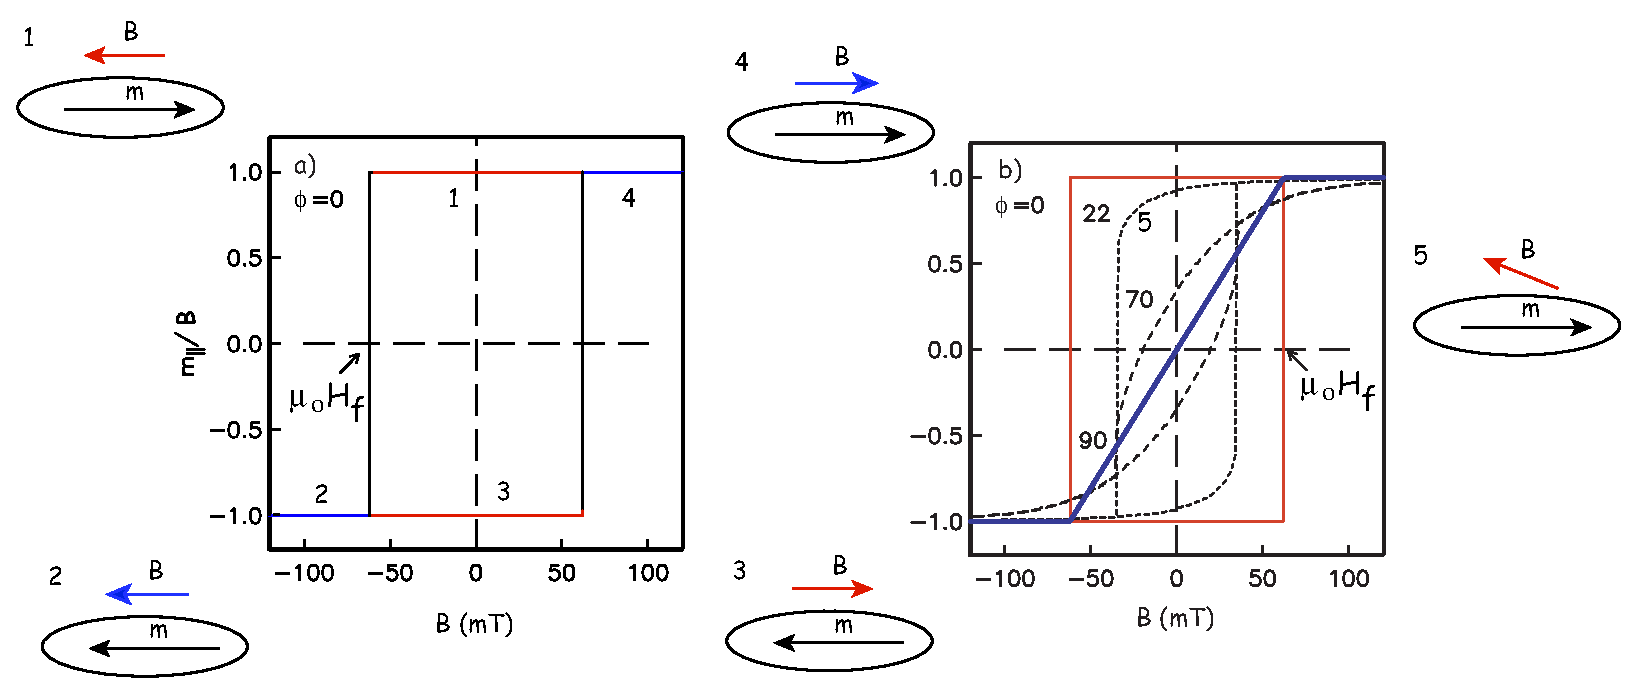
\includegraphics[width=14 cm]{EPSfiles/outerloop.eps}
\caption{ Moment measured for the particle ($\phi=0^{\circ}$) with applied field starting at 0 mT and increasing in the opposite directions along track \#1.  When the flipping field $\mu_oH_f$ is reached, the moment switches to the other direction along track \#2.  The field then switches sign and decreases along track \#3 to zero, then increases again to the flipping field.  The moment flips and the the field increases along track \#4. b) The component of magnetization  parallel to +B$_{max}$ versus $B$ for field applied with various angles $\phi$.  }
\label{fig:outerloop}
\end{figure}




Before we go on, it is useful to consider for a moment how 
\index{hysteresis!measurement of}
hysteresis measurements are made in practice.  
Measurements of magnetic moment $m$ as a function of applied field $B$ are made on a variety of instruments, such as a 
\index{magnetometer!vibrating sample}
\index{magnetometer!alternating gradient force}
vibrating sample magnetometer (VSM) or alternating gradient force magnetometer (AGFM).  In the latter, a specimen is placed on a thin stalk between pole pieces of a large magnet.  There is a probe mounted  behind the specimen that measures the applied magnetic field.  There are small coils on the pole pieces that modulate the gradient of the applied magnetic field (hence alternating gradient force).   The specimen vibrates in response to changing magnetic fields and the amplitude of the vibration is proportional to the moment in the axis of the applied field direction.   The vibration of the specimen stalk is measured and calibrated in terms of magnetic moment.  The magnetometer is only sensitive to the
induced 
component of $\m$ parallel to the applied field $\B_o$, which is  $m_{||}= m \cos \phi$ (because the off axis terms are squared and very small, hence can be neglected.) 
In the hysteresis experiment, therefore,  the moment parallel to the field $m_{||}$ is measured as a function of applied field $B$.  


\begin{figure}[h!tb]
%\epsfxsize 14cm
%\centering \epsffile{EPSfiles/sdloops.eps}
\centering  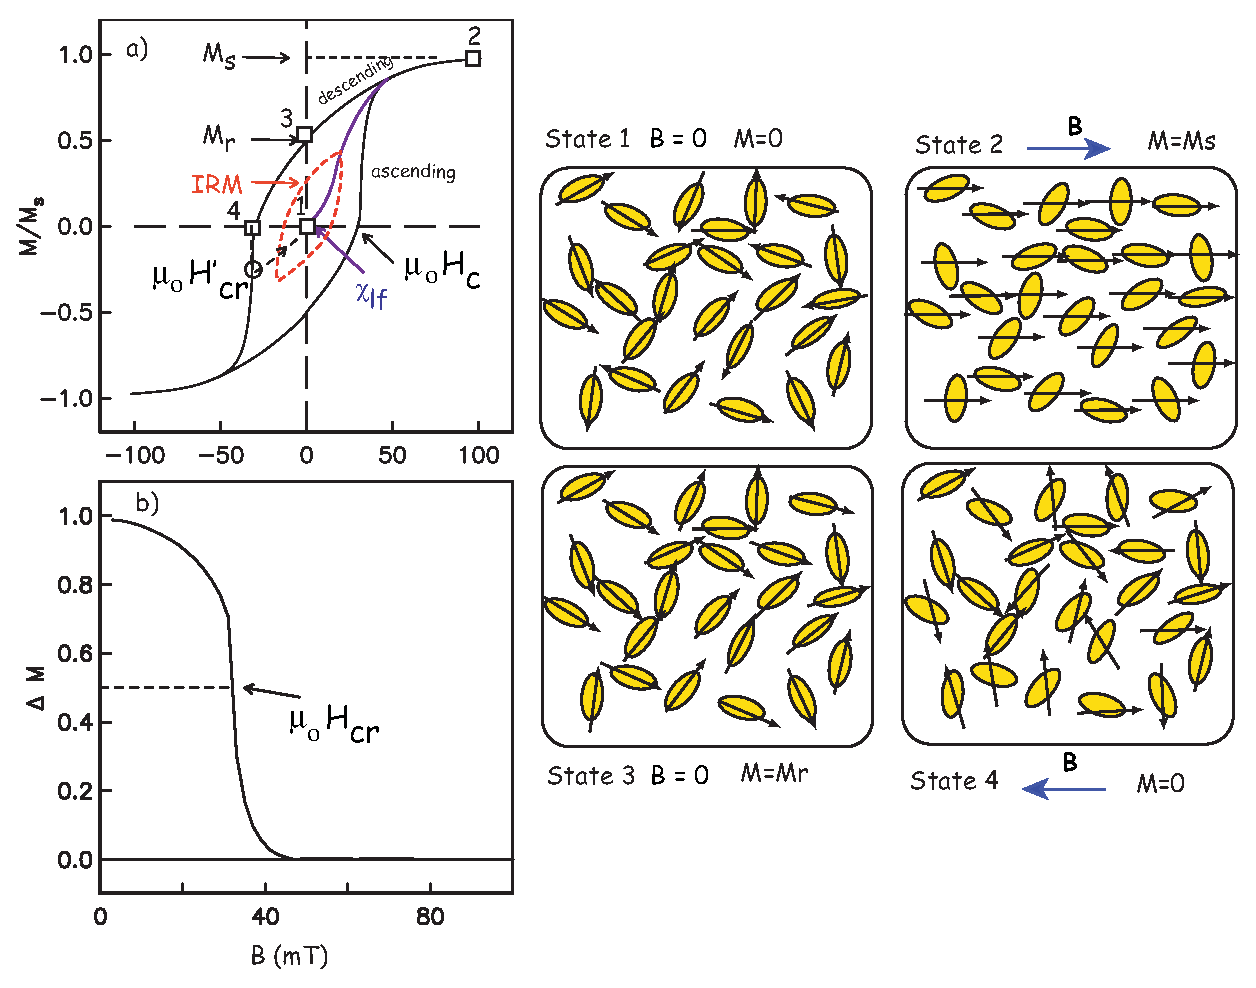
\includegraphics[width=14 cm]{EPSfiles/sdloops.eps}
\caption{a)  Net response of a random assemblage of  uniaxial single domain particles.  Snap shots of magnetization states (squares labelled 1 to 4)  for representative particles  are shown in the balloons labelled State 1- 4.   The initial demagnetized state is ``State 1''.  The initial slope as the field is increased from zero is the low-field susceptibility $\chi_{lf}$.      If the field returns to zero after some flipping fields have been exceeded, there is a net 
\index{magnetization!remanent!isothermal}
isothermal remanence (IRM).   When all the moments are parallel to the applied field (State 2), the magnetization is at saturation $M_s$. When the field is returned to zero, the magnetization is a saturation remanence ($M_r$; State 3).    When the field is applied in the opposite direction and has remagnetized half the moments (State 4), the field is the  bulk coercive field $\mu_oH_c$.   When a field is reached that when reduced to zero leaves zero net remanence, that field is  the coercivity of remanence (here labelled $\mu_oH_{cr}'$).    b)  Curve obtained by subtracting the ascending curve in a)  from the descending curve.  The field at which half the moments have flipped, leaving a magnetization of one half of saturation is another measure of the coercivity of remanence, here labelled $\mu_oH_{cr}$.}
\label{fig:sdloops}
\end{figure}


In rocks with an assemblage of randomly oriented particles with uniaxial anisotropy, we would measure the sum of all the millions of tiny individual loops.  A specimen from such a rock would yield a loop similar to that shown in Figure~\ref{fig:sdloops}a.  If the field is first applied to a demagnetized specimen, the initial slope is the (low field) 
\index{magnetic!susceptibility!low field}
magnetic susceptibility ($\chi_{lf}$) first introduced in  Chapter 1.   From the treatment in Section~\ref{sect:flipping} it is possible to derive the equation $\chi_{lf} = \mu_o M_s^2/3K_u$ for this initial (ferromagnetic) susceptibility (for more, see
\nocite{oreilly84}
\index{O'Reilly,  O.}
O'Reilly 1984). 



 If the field is increased beyond the flipping field of some of the magnetic grains and returned to zero, the net remanence is called an 
 \index{magnetization!remanent!isothermal}
{\it isothermal remanent magnetization} (IRM).  If the field is increased to $+B_{max}$, all the magnetizations are drawn into the field direction and the net magnetization is equal to the sum of all the individual magnetizations and is the {\it saturation magnetization} $M_s$.    When the field is reduced to zero, the moments relax back to their individual easy axes, many of which are at a high angle to the direction of the saturating field and cancel each other out.   A loop that does not achieve a saturating field (red in Figure~\ref{fig:sdloops}a is called a {\it minor hysteresis loop}, while one that does is called the {\it outer loop}. 
 
 
\begin{figure}[htb]
%\epsfxsize 7.75cm
%\centering \epsffile{EPSfiles/Bcr.eps}
\centering  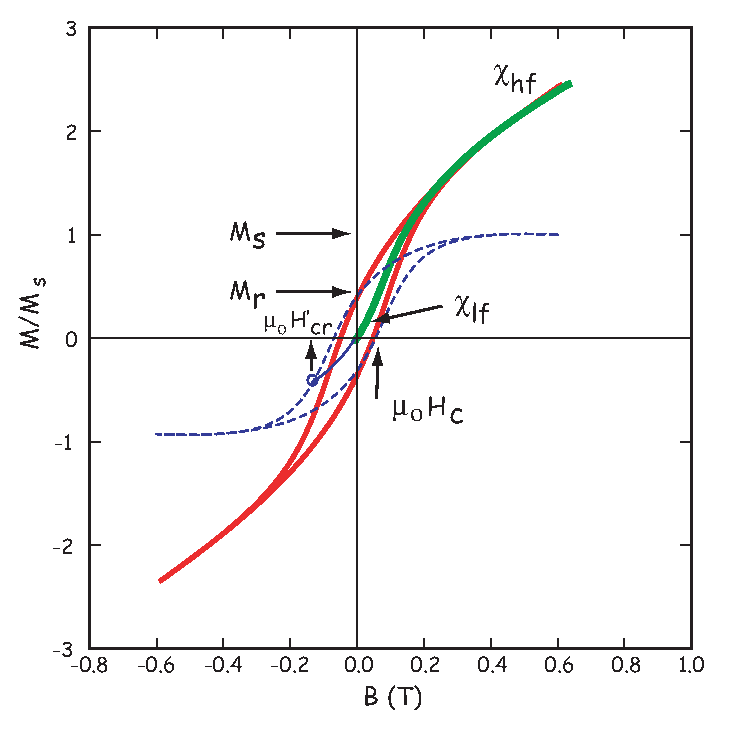
\includegraphics[width=7.75 cm]{EPSfiles/Bcr.eps}
\caption{Heavy green line: initial behavior of demagnetized specimen as applied field ramps up from zero field to a saturating field.  The initial slope is the initial or low-field susceptibility $\chi_{lf}$.  After saturation is achieved the slope is the high-field susceptibility $\chi_{hf}$ which is the non-ferromagnetic contribution, in this case the paramagnetic susceptibility (because $\chi_{hf}$ is positive.) The dashed blue line is the hysteresis loop after the paramagnetic slope has been subtracted.  Saturation magnetization $M_s$ is the maximum value of magnetization after slope correction.  Saturation remanence $M_r$ is the value of the magnetization remaining in zero applied field.  Coercivity ($\mu_o H_c$) and coercivity of remanence $\mu_oH_{cr}'$ are as in Figure 5.5a. }
 \label{fig:Bcr}
\end{figure}

%\clearpage

The net remanence after saturation is termed the 
 \index{magnetization!remanent!saturation}
{\it saturation remanent magnetization} $M_r$ (and sometimes the saturation isothermal remanence sIRM).  For a random assemblage of single domain uniaxial particles, $M_r/M_s$ = 0.5.   The field necessary to reduce the net moment to zero is defined as the 
\index{coercive field}
{\it coercive field} ($\mu_oH_c$) (or coercivity).  




The 
\index{coercivity!of remanence}
coercivity of remanence $\mu_o H_{cr}$ is defined as the magnetic field required to irreversibly flip half the magnetic moments (so the net remanence after application of a field equal to $-\mu_oH_{cr}$ to a saturation remanence is 0).  The coercivity of remanence is always greater than or equal to the coercivity and the ratio $H_{cr}/H_c$ for our random assemblage of uniaxial SD particles is 1.09
 \nocite{wohlfarth58}    
 \index{Wohlfarth, W.P.}
 (Wohlfarth, 1958).   Here we introduce two ways of estimating coercivity of remanence, illustrated in Figure~\ref{fig:sdloops}.  
 \index{coercivity!of remanence!estimation!ascending loop intercept method}
  If, after taking the field up to some saturating field $+B_{max}$, one first turned the field off (the descending curve), then increased the field in the opposite direction to the point labeled $\mu_oH'_{cr}$, 
and one were to then switch the field off again, the magnetization would follow the dashed curve up to the origin.   For single domain grains, the dashed curve would be  parallel to the lower curve (the ascending curve).  So, if one only measured the outer loop, one could estimate the coercivity of remanence by simply tracing the curve parallel to the lower curve (dashed line) from the origin to the point of intersection with the upper curve (circled in Figure~\ref{fig:sdloops}a).    This estimate is only valid for single domain grains, hence the prime in $\mu_oH_{cr}'$.   



 

 An alternative means of estimating coercivity of remanence  is to use  a so-called 
 \index{coercivity!of remanence!estimation!$\Delta M$ method}
 $\Delta M$ curve 
 \nocite{jackson90} 
 \index{Jackson, M.J.}
 (Jackson et al., 1990) which is obtained by subtracting the  ascending loop  from the descending loop (see  Figure~\ref{fig:sdloops}b).  When all the moments are flipped into the new field, the ascending and descending loops join together and $\Delta M$ is 0.  $\Delta M$ is at 50\% of its initial value at the field at which  half the  moments are flipped (the definition of coercivity of remanence); this field is here termed $\mu_oH_{cr}$.   
 



\subsection{Magnetic susceptibility}
\label{sect:chi}

Figure~\ref{fig:sdloops}a is the loop created in the  idealized case in which only uniaxial ferromagnetic particles participated in the hysteresis measurements; in fact the curve is entirely theoretical.  In ``real'' specimens there can be  paramagnetic, diamagnetic AND ferromagnetic particles and the loop may well look like that shown in Figure~\ref{fig:Bcr}.   The initial slope of a hysteresis experiment starting from a demagnetized state in which the field is ramped from zero up to higher values is the low field magnetic susceptibility or $\chi_{lf}$ (see Figure~\ref{fig:Bcr}).   If the field is then turned off, the magnetization will return again to zero.  But as the field increases passed the lowest flipping field, the remanence will no longer be zero but some isothermal remanence.    Once all particle moments have flipped and saturation magnetization has been achieved, the slope relating magnetization and applied field  reflects only the non-ferromagnetic (paramagnetic and/or diamagnetic)  susceptibility, here called
\index{magnetic!susceptibility!high field}
 {\it high field susceptibility}, $\chi_{hf}$.   In order to estimate the 
 \index{magnetization!saturation}
 saturation magnetization and the 
 \index{magnetization!remanent!saturation}
 saturation remanence, we must first subtract the high field slope.  So doing gives us the blue dashed line in Figure~\ref{fig:Bcr} from which we may read the various hysteresis parameters illustrated in Figure~\ref{fig:sdloops}b.  



\subsection{Cubic anisotropy}

In the case of  equant grains of magnetite for which magnetocrystalline anisotropy dominates, there are four easy axes, instead of two as in the uniaxial case (see Chapter 4).    The maximum angle $\phi$ between an easy axis and an applied field direction is 55$^{\circ}$.  Hence there is no individual loop that goes through the origin (see Figure~\ref{fig:cubic}).    A random assemblage of particles with 
\index{anisotropy!cubic}
cubic anisotropy will therefore have a much higher saturation remanence.  In fact, the theoretical ratio of $M_r/M_s$  for such an assemblage is 0.87, as opposed to 0.5 for the uniaxial case 
\nocite{joffe74}
\index{Joffe, I.}
\index{Heuberger, R.}
(Joffe and Heuberger, 1974).      
\begin{figure}[h!tb]
%\epsfxsize 6cm
%\centering \epsffile{EPSfiles/cubicloops.eps}
\centering  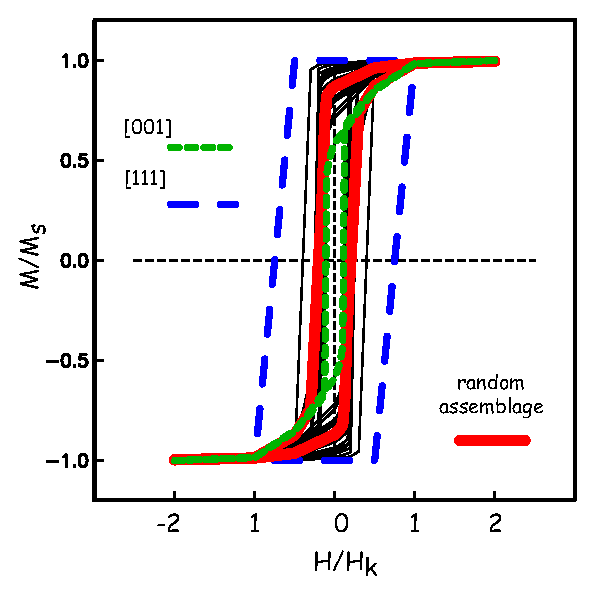
\includegraphics[width=6 cm]{EPSfiles/cubicloops.eps}
\caption{Heavy lines: theoretical behavior of cubic grains of magnetite.  Dashed lines are the responses along particular directions.  Light grey lines: hysteresis response for single particles with various orientations with respect to the applied field. [Figure from Tauxe et al., 2002.]}
\label{fig:cubic}
\end{figure}  
\nocite{tauxe02}


\begin{figure}[htb]
%\epsfxsize 12cm
%\centering \epsffile{EPSfiles/loops.eps}
\centering  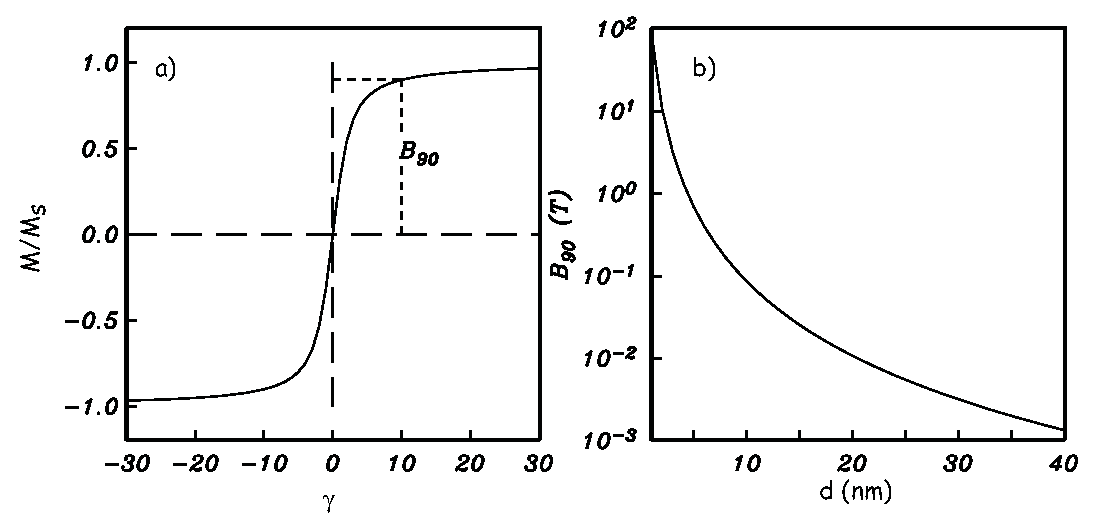
\includegraphics[width=12 cm]{EPSfiles/loops.eps}
\caption{a) The contribution of SP particles with saturation magnetization $M_s$ and cubic edge length $d$.  $\gamma = BM_s d^3/kT$.  There is no hysteresis.  b) The field at which the magnetization reaches 90\% of the maximum $B_{90}$ is when $ M_s d^3/kT\simeq 10$. [Figure from Tauxe et al.,  1996.] }
\label{fig:loops}
\end{figure}
\nocite{tauxe96}

\subsection {Superparamagnetic particles}
\label{sect:SP}

In 
\index{superparamagnetism}
superparamagnetic (SP) particles, the total magnetic energy $E_t=\epsilon_tv$ (where $v$ is volume) is balanced by thermal energy $kT$.  This behavior can be modeled using statistical mechanics  in a manner similar to that derived for paramagnetic grains in Section~\ref{sect:para} in Chapter 3 and summarized in Appendix~\ref{app:superparamagnetism}.  In fact, 


\begin{equation}
{M\over {M_s}} =
{ N(\hbox{coth }\gamma -
{
1\over{\gamma}
}), 
}
\label{eq:Lang1} 
\end{equation}
\noindent where $\gamma = { {M_sBv}\over {kT}} $ and $N$ is the number of particles of volume $v$, 
 is a reasonable approximation. 
The end result, Equation~\ref{eq:Lang1}, is the familiar 
\index{Langevin!function}
Langevin function from our discussion of  paramagnetic behavior (see Chapter  3); hence
the   term ``superparamagnetic'' for such particles.

 



The
contribution of SP particles for which the Langevin function is valid with given $M_s$ and $d$ is shown in Figure~\ref{fig:loops}a.
The field at which the population reaches 90\%
saturation $B_{90}$ occurs at $\gamma \sim 10$.  
Assuming particles of magnetite ($M_s$ = 480 mAm$^{-1}$) and room temperature 
($T=300$\deg K), $B_{90}$ can
be evaluated as a function of $d$ (see Figure~\ref{fig:loops}b). 
Because of its inverse cubic dependence on $d$, $B_{90}$ rises sharply with decreasing $d$ and is
hundreds of tesla for particles a few nanometers in size, approaching paramagnetic
values.    $B_{90}$ is a quick guide to the  SP slope (the SP susceptibility $\chi_{sp}$) contributing to the hysteresis response and was  used by Tauxe et al. (1996) \nocite{tauxe96} as a means of explaining distorted loops sometimes observed for populations of SD/SP mixtures.   $B_{90}$ (and $\chi{sp}$) is  very sensitive to particle size with very steep slopes for the particles at the SP/SD threshold.   The exact threshold size 
is still rather controversial, but Tauxe et al. (1996) argue that it is $\sim $ 20 nm. 
\eject

\begin{figure}[htb]
%\epsfxsize 14cm
%\centering \epsffile{EPSfiles/mdloop.eps}
\centering  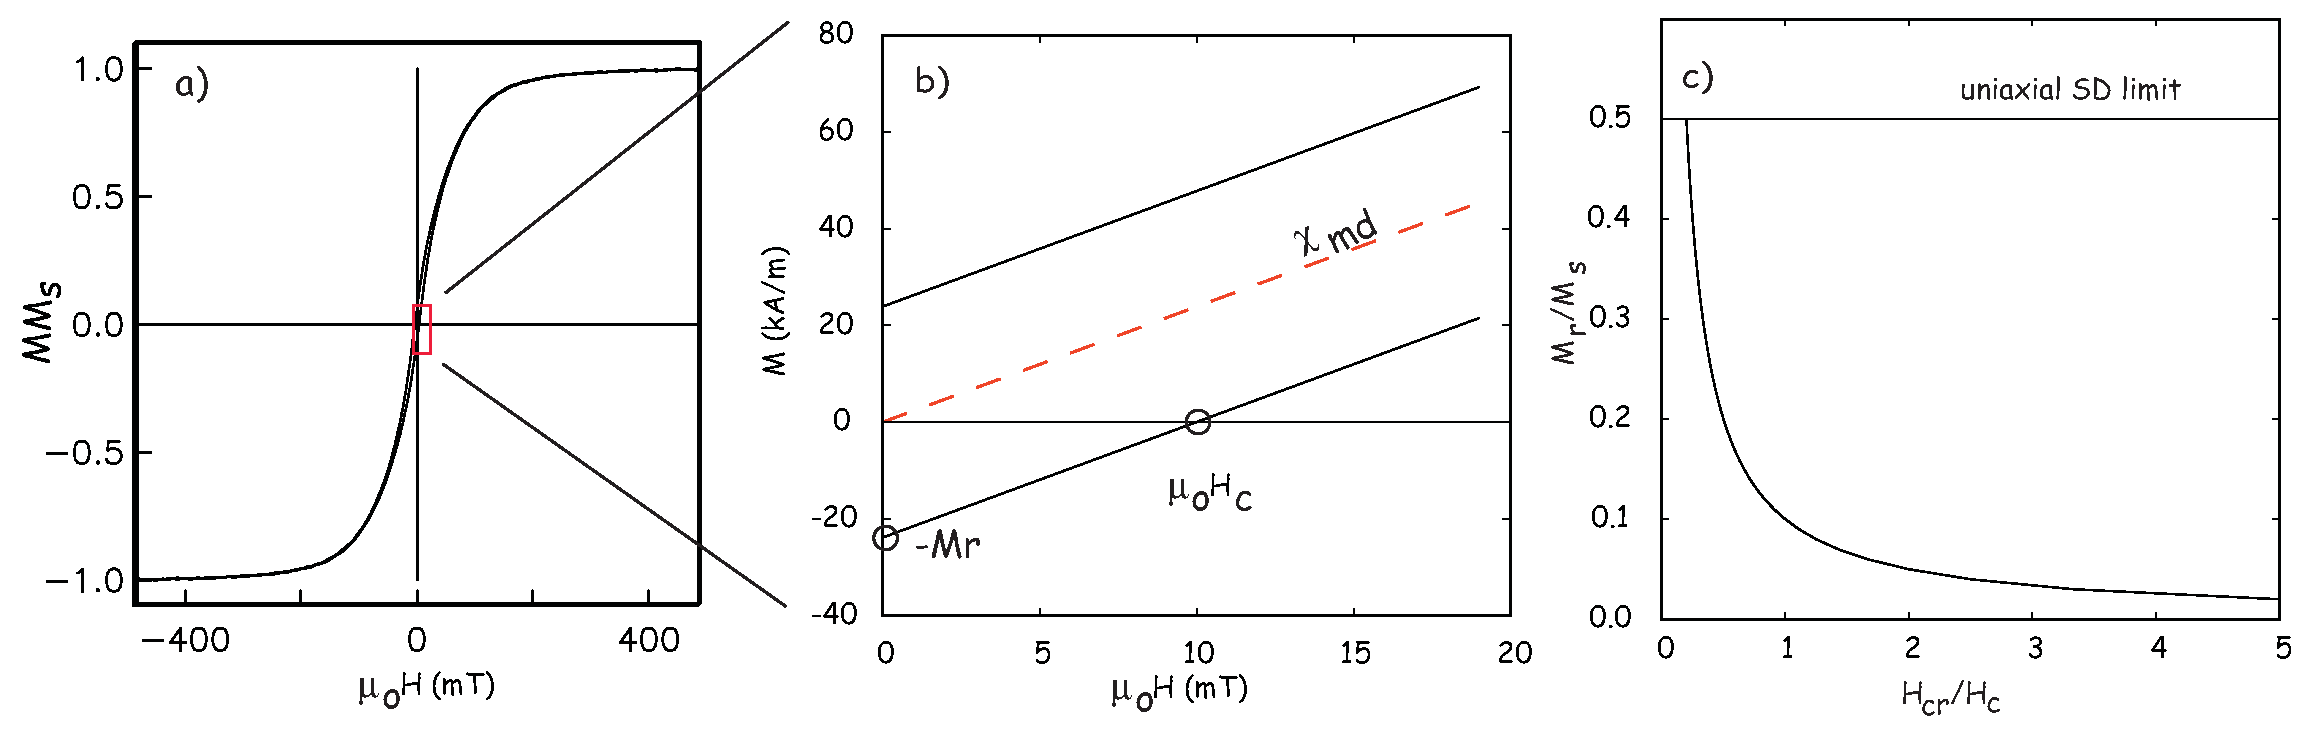
\includegraphics[width=14 cm]{EPSfiles/mdloop.eps}
\caption{a) Typical hysteresis loop from a multi-domain assemblage.   b) Theoretical behavior for the region in the inset to a).  c) Theoretical relationship between $M_r/M_s$ and $H_{cr}/H_c$ for constant $\chi_iH_c/M_s = 0.1$.   Heavy red line is the theoretical linear mixing curve of SD/MD end-members.  (see text) }
\label{fig:md}
\end{figure}


For low magnetic fields, the Langevin function can be approximated as $\sim 1\over 3 \gamma$.  So we have:
$$
{M\over {M_s}} = {1\over 3}  { {M_sBv}\over {kT}}.
$$
\noindent   If we substitute $\mu_o H$ for $B$ and rearrange this equation, we can get the superparamagnetic susceptibility $\chi_{sp}$ as:
\beq
{M\over H} =   { {\mu_o M_sv}\over {3kT}}.
\label{eq:chiSP}
\eeq

\noindent We can rearrange  Equation~\ref{eq:tau} in Chapter 4 to solve for the volume at which a uniaxial grain passes through the superparamagnetic threshold we find:  

$$
{v_b } ={{ \ln (C\tau)}\over{K_u}}.
$$
\noindent Finally, we  can substitute this volume into Equation~\ref{eq:chiSP} as the maximum volume of an SP grain, giving us:

\beq
\chi_{sp} = { {\mu_o M_s^2 \ln (C\tau)}\over {3K_u} }.
\label{eq:chiSP1}
\eeq

\noindent Comparing this expression with that derived for ferromagnetic susceptibility in Section~\ref{sect:uniaxial}, we find that $\chi_{sp}$ is a factor of $\ln(C\tau)\simeq 27$ larger than the equivalent single domain particle.  



 \begin{figure}[htb]
%\epsfxsize 12cm
%\centering \epsffile{EPSfiles/void.eps}
\centering  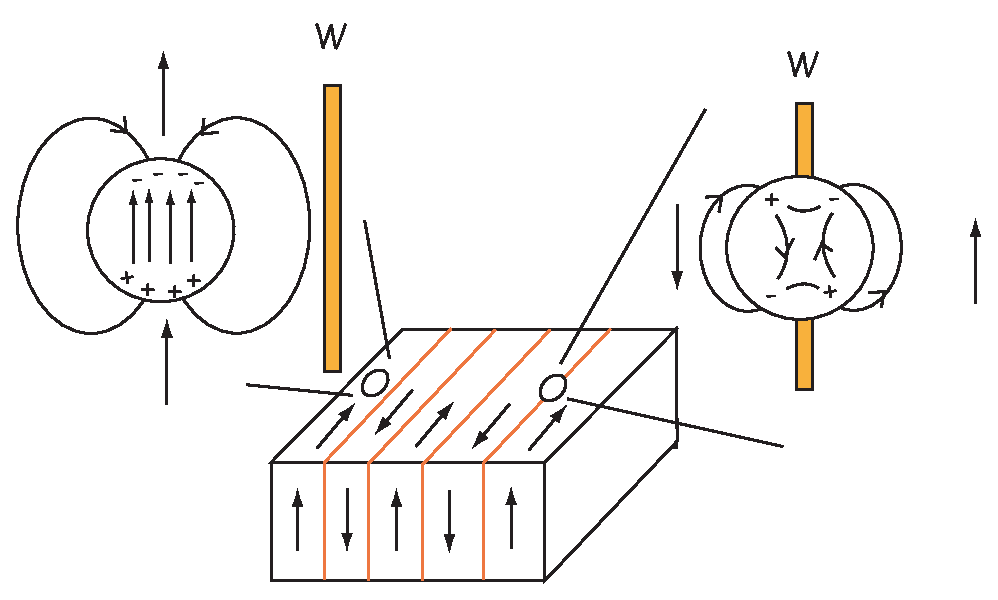
\includegraphics[width=12 cm]{EPSfiles/void.eps}
\caption{ Interaction of a domain wall and a void.  When the void is within a domain, free poles create a magnetic field which creates a self energy (Chapter 4).  When a domain wall intersects the void, the self-energy is reduced.  There are no exchange or magnetocrystalline anisotropy energy terms within the void, so the wall energy is reduced.}
\label{fig:void}
\end{figure}




\subsection{Particles with domain walls}
\label{sect:day}


Moving domain walls around is much easier than flipping the magnetization of an entire particle coherently.   The reason for this is the same as the reason that it is easier to move a rug by lifting up a small wrinkle and pushing that through the rug, than to drag the whole rug by the same amount.  Because of the greater ease of changing magnetic moments in multidomain (MD) grains, they have lower coercive fields and saturation remanence is also much lower than for uniformly magnetized particles (see typical MD hysteresis loop in Figure~\ref{fig:md}a.)

The key to understanding multi-domain hysteresis is the reduction in multi-domain magnetic susceptibility  $\chi_{md}$ from ``true'' magnetic susceptibility ($\chi_i$) because of self-demagnetization.  The true susceptibility would be that obtained by measuring the magnetic response of a particle to the internal field $\H_i$ (applied field minus the demagnetizing field $-N\M$ -- see Section~ \ref{sect:shape}; see 
\index{Dunlop, D.J.}
Dunlop 2002a).  \nocite{dunlop02a}
  Recalling that the demagnetizing factor is $N$, the so-called {\it screening factor} $f_s$ is $(1 + N\chi_i)^{-1}$ and $\chi_{md} = f_s \chi_i $.
If we assume that $\chi_{md}$ is linear for fields less than the coercivity, then by definition $\chi_{md} = {{ M_r}\over{H_c} }$ (see Figure~\ref{fig:md}b).  From this, we get:

$$
{{M_r}\over{M_s}} = \chi_{md} { H_c\over{M_s}} = f_s \chi_i { H_c\over{M_s}}.
$$
\noindent In the case of multi-domain susceptibility,  $\chi_i$ is much larger than $\chi_{md}$ and $M_r = { {H_c}\over{N}}$.    

By a similar argument,
\index{coercivity!of remanence}
coercivity of remanence ($H_{cr}$) is suppressed by the  screening factor which gives coercivity so:

$$
H_c =  f_s H_{cr}, 
$$
\noindent    from which we get the ratio:

$$
{H_{cr}\over{H_c}} = f_s. 
$$
\noindent  

\noindent Putting all this together leads us to the remarkable relationship noted by 
\index{Day, R.}
Day et al. (1977; see also 
\index{Dunlop, D.J.}
Dunlop 2002a): \nocite{day77,dunlop02a} 

\begin{equation}
{ M_r\over{M_s}} \cdot { H_{cr}\over{H_c}} = \chi_i { H_c\over {M_s}}.
\label{eq:day}
\end{equation} 

When  $\chi_i { H_c\over {M_s}}$ is constant, Equation~\ref{eq:day} is a hyperbola.   
For a single mineralogy, we can expect $M_s$ to be constant, but $H_c$ depends on grain size and the state of stress which are unlikely to be constant for any natural population of magnetic grains.   
\index{Dunlop, D.J.}
Dunlop (2002a) \nocite{dunlop02a} argues that if the main control on susceptibility and coercivity is domain wall motion through a terrain of variable wall energies, then $\chi_i$ and $H_c$ would be inversely related and gives a tentative theoretical value for $\chi_iH_c$  in magnetite of  about 45 kAm$^{-1}$.   This, combined with the value of $M_s$ for magnetite of 480  kAm$^{-1}$  gives a value for $\chi_i { H_c\over {M_s}} \sim 0.1$.  
When anchored by the theoretical maximum for uniaxial single domain ratio of $M_r/M_s = 0.5$, we get the curve shown in Figure~\ref{fig:md}c.   The major control on coercivity is grain size, so the trend from the SD limit down toward low $M_r/M_s$ ratios is increasing grain size.  

   
  

There are several possible causes of variability in wall energy within a magnetic grain, for example, voids, lattice dislocations, stress, etc.  The effect of voids is perhaps the easiest to visualize, so we will consider voids as an example of why wall energy varies as a function of position within the grain.   We show a particle with lamellar domain structure and several voids in Figure~\ref{fig:void}.  When the void occurs within a uniformly magnetized domain (left of figure), the void sets up a demagnetizing field as a result of the free poles on the surface of the void.  There is therefore, a self-energy associated with the void.   When the void is traversed by a wall, the free pole area is reduced, reducing the demagnetizing field and the associated self-energy.  Therefore, the energy of the void is reduced by having a wall bisect it.  Furthermore, the energy of the wall is also reduced, because the area of the wall in which magnetization vectors are tormented by exchange and magnetocrystalline energies is reduced.  The wall gets a ``free'' spot if it bisects a void.  The wall energy $E_w$ therefore is lower as a result of the void.  




\begin{figure}[htb]
%\epsfxsize 14cm
%\centering \epsffile{EPSfiles/wallenergy.eps}
\centering  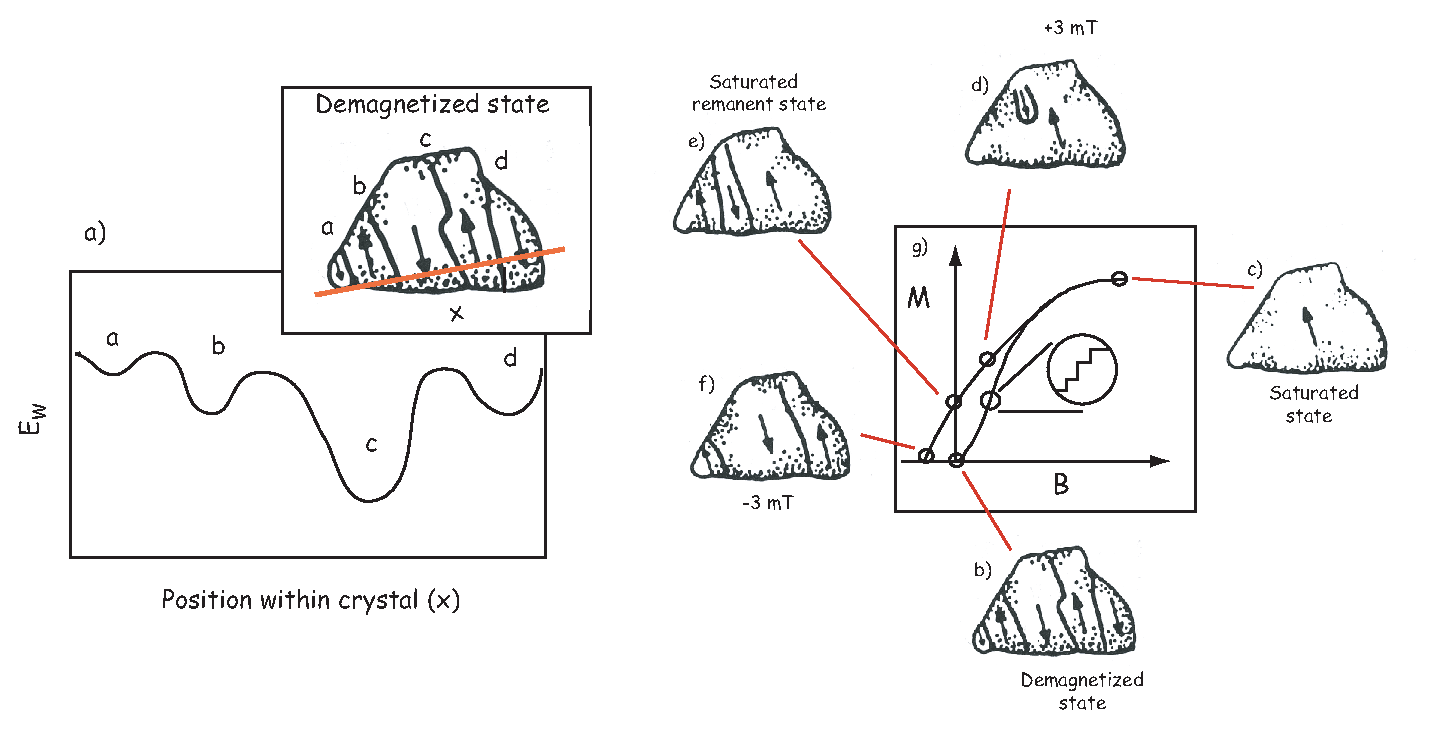
\includegraphics[width=14 cm]{EPSfiles/wallenergy.eps}
\caption{a) Schematic view of wall energy across a transect of a multi-domain grain.  Inset: Placement of domain walls in the demagnetized state.  [Domain observations from Halgedahl and Fuller,  1983.] b-g) Schematic view of the magnetization process in MD grain shown in previous figure.  b) Demagnetized state, c) in the  presence of a saturating field, d) field lowered to +3 mT, e) remanent state, f) backfield of -3 mT, g) resulting loop.  Inset shows detail of domain walls moving by small increments called Barkhausen jumps.  [Domain wall observations from Halgedahl and Fuller, 1983; schematic loop after O'Reilly, 1984.]}
\label{fig:wallenergy}
\end{figure}
\nocite{oreilly84}\nocite{halgedahl83}



In  Figure~\ref{fig:wallenergy}, we show a sketch of a hypothetical transect of  $E_w$ across a particle.  There are four LEMs labelled a-d.   Domain walls will distribute themselves through out the grain in order to minimize the net magnetization of the grain and also to try to take advantage of LEMs in wall energy.   

Domain walls move in response to external magnetic fields (see Figure~\ref{fig:wallenergy}b-g).   Starting in the demagnetized state  (Figure~\ref{fig:wallenergy}b), we apply a magnetic field that increases to saturation (Figure~\ref{fig:wallenergy}c).    As the field increases, the domain walls move in sudden jerks as each successive local wall energy high is overcome.  This process, known as {\it Barkhausen jumps},  leads to the stair-step like increases in magnetization (shown in the inset of  Figure~\ref{fig:wallenergy}g).  At saturation, all the walls have been flushed out of the crystal and it is uniformly magnetized.  When the field decreases again, to say +3 mT (Figure~\ref{fig:wallenergy}d), domain walls begin to nucleate, but because the energy of nucleation is larger than the energy of denucleation, the grain is not as effective in cancelling out the net magnetization, hence there is a net saturation remanence (Figure~\ref{fig:wallenergy}e).  The  walls migrate around as a magnetic field is applied in the opposite direction (Figure~\ref{fig:wallenergy}f) until there is no net magnetization.  The difference in nucleation and denucleation energies was called on by \nocite{halgedahl83}
\index{Halgedahl, S.}
\index{Fuller, M.}
Halgedahl and Fuller (1983) to explain the high stability observed in some large magnetic grains. 

\section{Hysteresis of mixtures of SP, SD and MD grains}
\label{sect:mixtures}

\index{Day, R.}
Day et al. (1977) \nocite{day77}  popularized the use of diagrams like that shown in Figure~\ref{fig:md}c which are known as
\index{diagrams!Day}
{\it Day diagrams}.   They placed quasi-theoretical bounds on the plot whereby points with $M_r/M_s$ ratios above 0.5 were labelled  single domain  (SD), and points falling in the box bounded by $0.5>M_r/M_s>0.05$ and $1.5<H_{cr}/H_c < 5$ were labelled
 \index{pseudo-single domain}
{\it pseudo-single domain}  (PSD).  Points with $M_r/Ms$ below 0.05 were labelled multi-domain (MD).    This paper has been cited over 800 times in the literature and the Day plot still serves as the principle way that rock and paleomagnetists determined domain state and grain size.  

The problem with the Day diagram is that virtually all paleomagnetically useful specimens yield hysteresis ratios that fall within the PSD box.  In the early 90s, paleomagnetists began to realize that many  things besides the trend from SD to MD behavior that  control where points fall on the Day diagram.   
\index{Pick, T.}
\index{Tauxe, L.}
Pick and Tauxe (1994) \nocite{pick94} pointed out that mixtures of SP and SD grains would have reduced $M_r/M_s$ ratios and enhanced $H_{cr}/H_c$ ratios. 
\index{Tauxe, L.}
 Tauxe et al. (1996) \nocite{tauxe96} modelled distributions of SP/SD particles and showed that the SP-SD trends always fall above those observed from MD particles (modelled in Figure~\ref{fig:md}c).  

\index{Dunlop, D.J.}
Dunlop (2002a)  \nocite{dunlop02a} argued  that because $M_r$ for SP grains is zero, the  suppression of the ratio $M_r/M_s$ is directly proportional to the volume fraction of the SP particles.  Moreover, 
\index{coercivity!of remanence}
coercivity of remanence remains unchanged, as it is entirely due to the non-SP fraction.    Deriving the relationship of coercivity, however, is not so simple.   It depends on the superparamagnetic susceptibility ($\chi_{sp}$), which in turn depends on the size of the particle and also the applied field  (see Section~\ref{sect:SP}).    In his simplified approach, Dunlop could only use a single (small) grain size, whereas in natural samples,  there will always be a distribution of grain sizes.     It is also important to remember that  volume goes as the cube of the radius and for a mixture to display any SP suppression of $M_r/M_s$ almost all of the particles must be SP.  It is impossible that these would all be of a single radius (say 10 or 15 nm); there must be a distribution of sizes.  Moreover, Dunlop (2002a) neglected the complication in SP behavior as the particles reach the SD threshold size, whereas it is expected that many (if not most) natural samples containing  both SP and SD grain sizes will have a large volume fraction of the larges SP sizes, making their neglect problematic. 

\begin{figure}[h!tb]
%\epsfxsize 14cm
%\centering \epsffile{EPSfiles/forcprinc.eps}
\centering  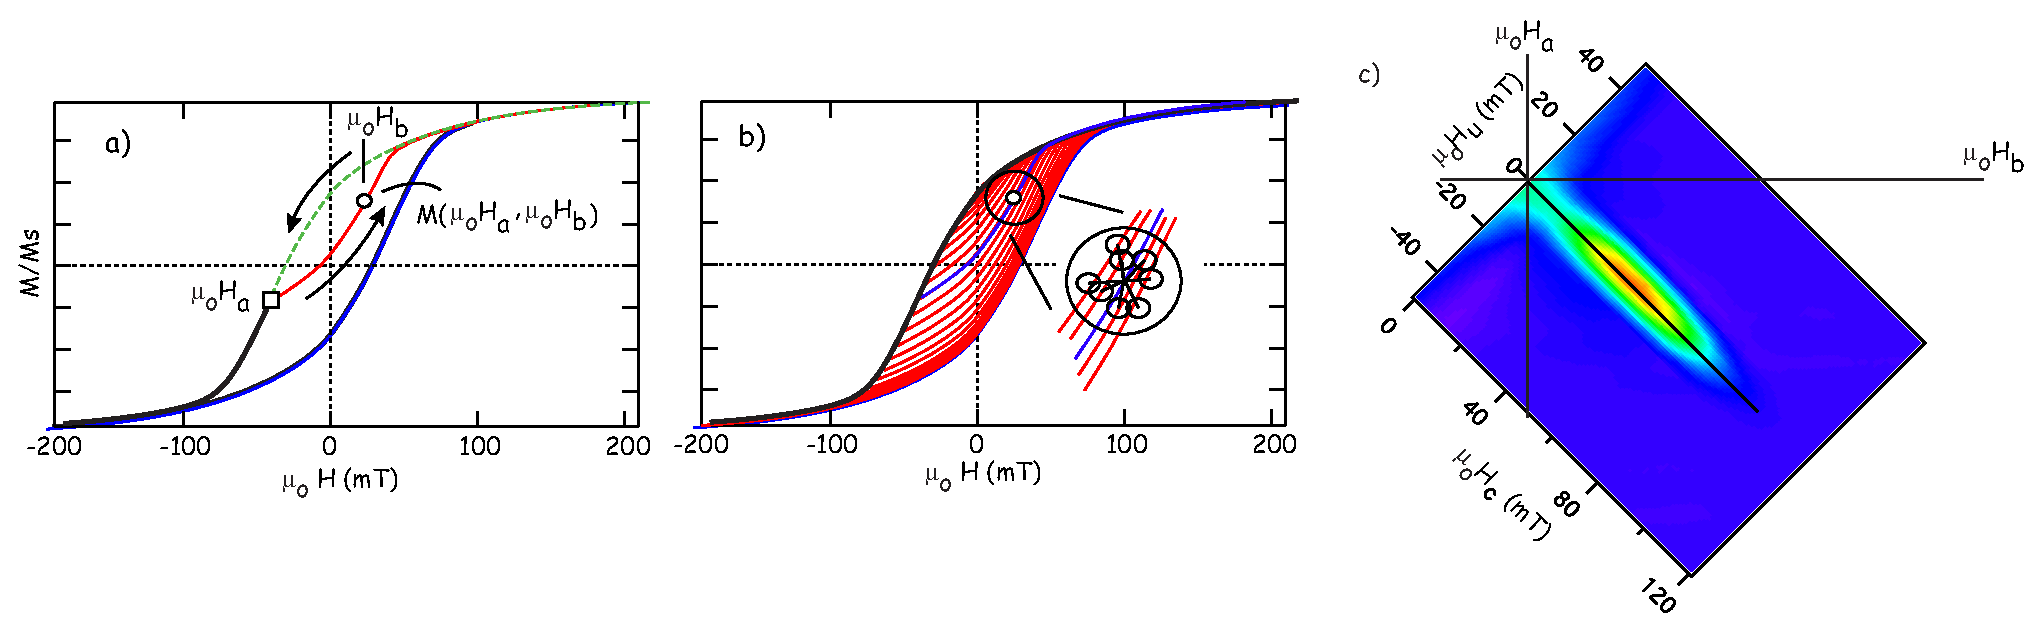
\includegraphics[width=14 cm]{EPSfiles/forcprinc.eps}
\caption{a) Dashed line is the descending magnetization curve taken from a saturating field to some field $H_a$.  Red line is the first order reversal curve (FORC) from $H_a$ returning to saturation.   At any field $H_b>H_a$ there is a value for the magnetization $M(H_a,H_b)$.  b) A series of FORCs for a single domain assemblage of particles.  At any point  there are a set of related ``nearest neighbor'' measurements (circles in inset).  A least-squares fit to Equation 5.8 can be determined for each point.    c) A contour plot of the FORC density surface for data in b).   Specimen is  of the Tiva Canyon Tuff, courtesy of the Institute for Rock Magnetism.   }
\label{fig:forcprinc}
\end{figure}


Hysteresis ratios of mixtures of SD and MD particles will also plot in the ``PSD'' box.  Dunlop (2002a) derived the theoretical behavior of such mixtures on the Day diagram.    The key equations are 1) Equation 9 from Dunlop (2002) which governs the behavior of the ratio $M_r/M_s$ as a function of the volume fraction of single domain material ($f_{SD}$) and multi-domain material ($f_{MD}$): 

$$
{M_r/M_s} = f_{SD} (M_r/Ms)_{SD} + f_{MD} (M_r/M_s)_{MD}, 
$$

\noindent   2) Equation 10 from Dunlop (2002a) which governs the behavior of coercivity:

$$
H_c = [f_{SD} \chi_{SD} (H_c)_{SD} + f_{MD} \chi_{SD} \chi_{MD} (H_c)_{MD}] / (f_{SD} \chi_{SD} + f_{MD} \chi_{MD}), 
$$

\noindent and 3) Equation 11 from Dunlop (2002a) which governs the behavior of coercivity of remanence in SD/MD mixtures:

$$
{H_{cr} =}  {  f_{SD}( \chi_r)_{SD} (H_{cr})_{SD} +  f_{MD}( \chi_r)_{MD} (H_{cr})_{MD} } \over { f_{SD} (\chi_r)_{SD} + f_{MD} (\chi_r)_{MD} }
$$

\noindent where $\chi_{SD}$ and $\chi_{MD}$ are the susceptibilities of the SD and MD fractions respectively and $(\chi_r)_{SD}$  and $(\chi_r)_{MD}$ are the $M_r$ vs $H_{cr}$ slopes of the SD and MD remanences respectively.   What we need to calculate the SD/MD mixing curve are values for the  various parameters  for single domain and multi domain end-members.   These were measured empirically for the MV1H bacterial magnetosomes (see Chapter 6) and  commercial magnetite (041183 of Wright Company) by    Dunlop and Carter-Stiglitz (2006) \nocite{dunlop06}  and shown in Table~\ref{tab:end members}.    Using the linear mixing model of Dunlop (2002a), we  plot the theoretical mixing curve predicted for these empirically constrained  end-members as the heavy red line in Figure~\ref{fig:md}c.    

\begin{table}
\caption{Empirical values for hysteresis parameters measured for single domain (SD) and multi-domain (MD) end-members of  Dunlop and Carter-Stiglitz (2006).}
\label{tab:endmembers}
\begin{tabular}{ llllll   }
\hline
SD/MD& $M_r/M_s$ & $\chi$ (A m$^{-1}$T$^{-1}$) & $\chi_r$ (MA m$^{-1}$T$^{-1}$)&$ \mu_o H_c$ (mT) &$ \mu_o H_{cr}$ (mT)\\
\hline
SD & 0.5 &  5.2&  4.55&46 & 52.5\\
MD & 0.02 & 4.14 & 0.88 &5.56 &26.1\\
\hline
\end{tabular}
\end{table}



% but the relationships are highly non-linear and are solved by trial and error.    Moreover, there are many embedded (and untestable) assumptions involved in these curves.      

If a population of SD particles are so closely packed as to influence one another, there will be an effect of particle interaction.  This will also tend to suppress the $M_r/M_s$ ratio, drawing the hysteresis ratios down into the PSD box.  
Finally, the PSD box could be populated by pseudo-single domain grains themselves.  Here we will dwell for a moment on  the meaning of the term ``pseudo-single domain'', which  has evolved from the original posed by 
\index{Stacey, F.}
Stacey (1961; see  discussion in 
\nocite{tauxe02}
\index{Tauxe, L.}
Tauxe et al. 2002). \nocite{stacey61,tauxe02}  In an attempt to explain trends in TRM acquisition Stacey envisioned that irregular shapes caused unequal domain sizes, which would give rise to a net moment that was less than the single domain value, but considerably higher than the very low efficiency expected for large MD grains.    The modern interpretation of PSD behavior is complicated micromagnetic structures that form between classic SD (uniformly magnetized grains) and MD (domain walls) such as the flower or vortex remanent states (see, e.g., Figure~\ref{fig:nonuniform} in Chapter 4).   
Taking all these factors into account means that interpretation of the Day diagram is far from unique.   The simple calculations of Dunlop (2002a) are likely to be  inappropriate for almost all natural samples.  






\section{First order reversal curves}


Hysteresis loops can yield a tremendous amount of  information yet much of this is lost by simply estimating the set of parameters $M_r, M_s,  H_{cr}, H_c, \chi_i, \chi_{hf}$, etc.   
\nocite{mayergoyz86}
\index{Mayergoyz, I.D.}
Mayergoyz (1986)    developed a method using  what are known as   {\it First Order Reversal Curves} or FORCs to represent hysteresis data.  The most recent way of dealing with
\index{diagrams!FORC}
 FORCs is that of
 \nocite{harrison08}
 \index{Harrison, R.J.}
 \index{Feinberg, J.M.}
  Harrison and Feinberg (2008)  which is illustrated in Figure~\ref{fig:forcprinc}.  In the FORC experiment,  a specimen is subjected to a saturating field,  as in most hysteresis experiments.  The field is lowered to some field $\mu_oH_a$, then increased again through some value $\mu_oH_b$  to saturation (see Figure~\ref{fig:forcprinc}a).   The magnetization curve between $\mu_o H_a$ and $\mu_oH_b$ is a ``FORC''.  A series of FORCs (see Figure~\ref{fig:forcprinc}b) can be generated to the desired resolution.  


 
 \begin{figure}[h!b]
%\epsfxsize 14cm
%\centering \epsffile{EPSfiles/m428.eps}
\centering  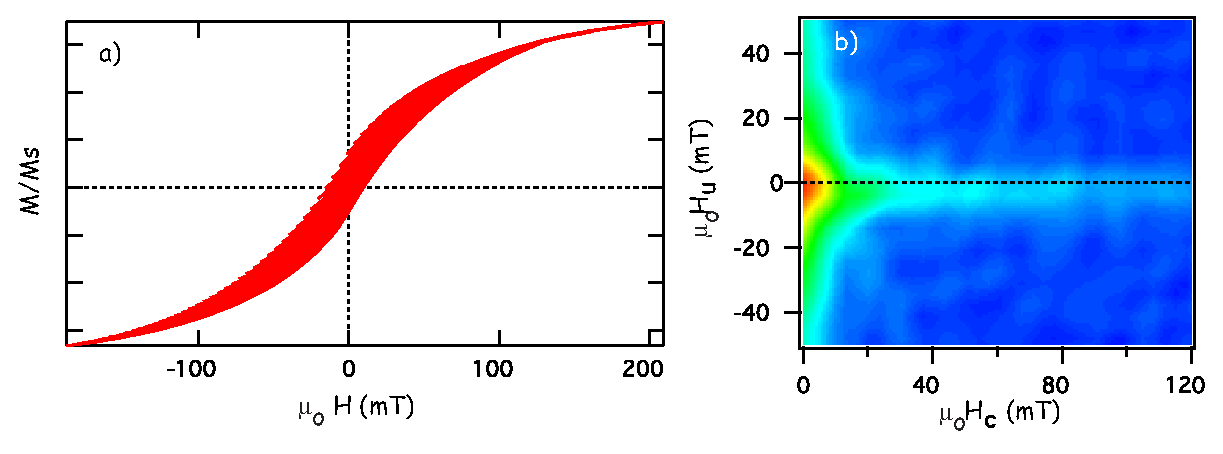
\includegraphics[width=14 cm]{EPSfiles/m428.eps}
\caption{a)  A series of FORCs for a ``pseudo-single domain'' specimen.  b) FORC diagram for data in a).   Specimen  is  of the Stillwater Layered Intrusion, courtesy of J.S. Gee.   }
\label{fig:forcpsd}
\end{figure}


To transform FORC data into some useful form, Harrison and Feinberg (2008) use a locally-weighted regression smoothing technique (LOESS).   For a given measurement point $P$ LOESS fits a second-order polynomial function of the form

\begin{equation}
M(H_a,H_b)= a_1 + a_2H_a + a_3H_a^2 + a_4H_b +a_5H_b^2 +a_6H_aH_b,
\label{eq:forc}
\end{equation}

\noindent  to the measured magnetization surface in a specified region (for example the circle shown in Figure~\ref{fig:forcprinc}b) where the $a_i$ are fitted coefficients.     The LOESS technique takes a user defined number of  the nearest neighbors (see inset to Figure~\ref{fig:forcprinc}b) for an arbitrary shaped region over which the data are smoothed.    
The coefficient $-a_6(H_a,H_b)$ is  the FORC density at the point.    A FORC diagram is the contour plot  of the FORC densities, rotated such that $\mu_oH_c = \mu_o(H_b-H_a)/2$ and $\mu_oH_u = \mu_o(H_a+H_b)/2$.    Please note that because $H_a<H_b$, data are only possible for positive $H_c$.  
 

\begin{figure}[htb]
%\epsfxsize 10cm
%\centering \epsffile{EPSfiles/ZFORC.eps}
\centering  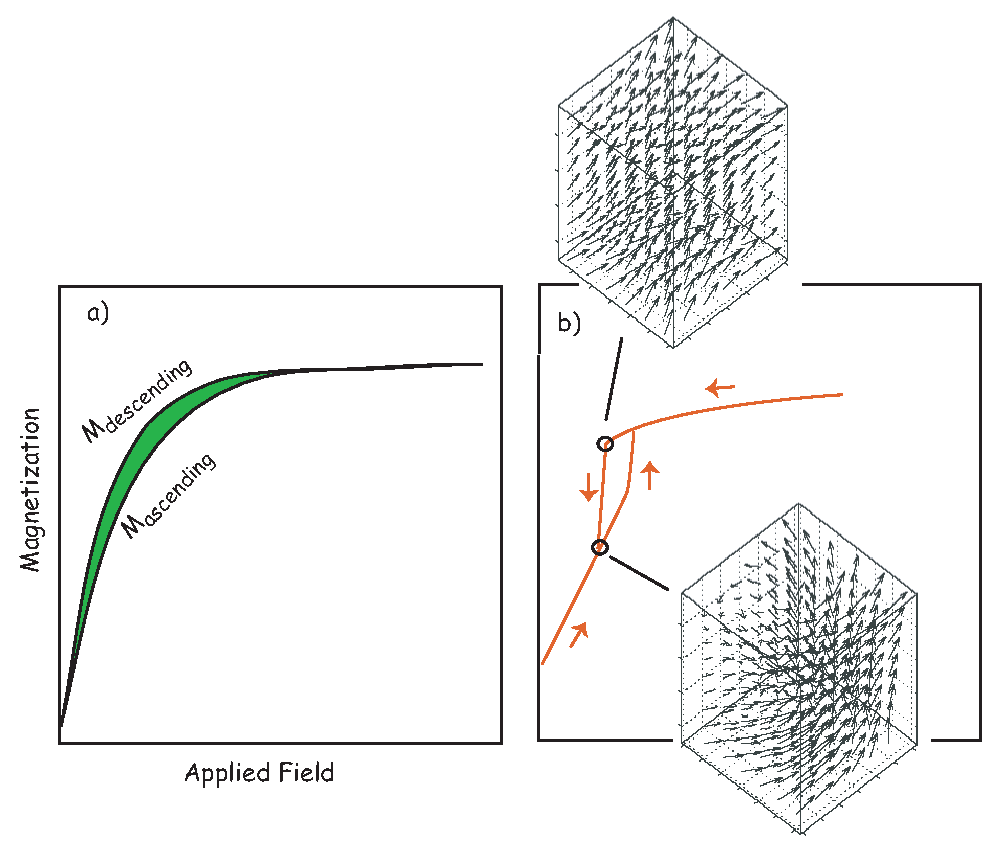
\includegraphics[width=10 cm]{EPSfiles/ZFORC.eps}
\caption{a) Illustration of a Zero FORC (ZFORC) whereby the descending loop from saturation is terminated at zero field and the field is then ramped back up to saturation.  The  transient hysteresis (TH) of 
Fabian (2003) is the shaded area between the two curves.  b) Micromagnetic model of a ZFORC for a 100 nm cube of magnetite.  Two snap shots of the internal magnetization on the descending and ascending loops are shown in the insets.  [Figure redrawn from Yu and Tauxe, 2005.] }
\label{fig:ZFORC}
\end{figure}
\nocite{yu05b}
\nocite{fabian03} 

 Imagine we travel down the descending magnetization curve (dashed line in Figure~\ref{fig:forcprinc}a) to a particular field $\mu_o H_a $ less than the smallest flipping field in the assemblage.   If the particles are single domain, the behavior is reversible and the first  FORC will travel back up the descending curve.  It is only when $|\mu_o H_a|$ exceeds the flipping field of some of the particles that the FORC will trace a new curve on the inside of the hysteresis loop.  In the simple single domain, non-interacting,  uniaxial magnetite case, the FORC density in the quadrants where $H_a$ and $H_b$ are of the same sign must be zero. Indeed, FORC densities will only be non-zero for the range of flipping fields  because these are the bounds of the flipping field distribution.      So the diagram in Figure~\ref{fig:forcprinc}c is nearly that of an ideal uniaxial SD distribution.  
 
 Consider  now the case in which a specimen has magnetic grains with non-uniform magnetizations such as vortex structures or domain walls.   Walls and vortices can move much more easily than flipping the moment of an entire grain coherently.  In fact,  they begin to move in small jumps (from LEM to LEM) as soon as the applied field changes.  If a structure nucleates while the field is decreasing and  the field is then ramped back up, the magnetization curve will not be reversible, even though the field never changed sign or approached the flipping field for coherent rotation.   The resulting FORC for such behavior would have much of the ``action'' in the region where $H_a$ is  positive.   When transformed to $H_u$ and $H_c$, the diagram will have the high densities for small $H_c$ but over a range of  $\pm H_u$.  The example shown in   Figure~\ref{fig:forcpsd} is of a specimen that has been characterized as ``pseudo-single domain''.  The FORC diagram in Figure~\ref{fig:forcpsd}b has some of the FORC densities concentrated along the $H_c$ axis characteristic  of single domain specimens (e.g., Figure~\ref{fig:forcprinc}c), but there is also concentration along the $H_u$ axis characteristic of PSD and MD specimens.       
 



  In many cases the the most interesting thing one learns from FORC diagrams is the degree to which there is irreversible behavior  when the field is reduced to zero then ramped back up to saturation (see Figure~\ref{fig:ZFORC}).  Such irreversible behavior in what 
  \nocite{yu05b} 
  \index{Yu, Y.}
  \index{Tauxe, L.}
  Yu and Tauxe (2005) call the ``Zero FORC'' or ZFORC  can arise from particle interactions, domain wall jumps or from the formation and destruction of vortex structures in the magnetic grains.   

\nocite{fabian03} 
\index{Fabian, K.L.}
Fabian (2003) defined a parameter called ``transient hysteresis''  which is the area between the ascending and descending loops of a ZFORC (shaded area in Figure~\ref{fig:ZFORC}).    This is defined as:

$$
TH= \mu_o\sum_0^{H_s} [M_{descending} - M_{ascending}] \cdot \Delta H.
$$
\noindent  where $\Delta H$ is the field increment used in the hysteresis measurement.   When normalized by $M_s$, TH has units of tesla.    
Transient hysteresis is thought to result  from self demagnetization, for example  shifting of domain walls or the formation and destruction of vortex structures.  An example of what might be causing transient hysteresis at the macro scale is shown for micromagnetic modelling of a  single particle in Figure~\ref{fig:ZFORC}b 
\nocite{yu05b}
\index{Yu, Y.}
\index{Tauxe, L.}
(Yu and Tauxe, 2005).   The ZFORC starts and ends at saturation.  On the descending loop, a vortex structure suddenly forms, at the point on the hysteresis loop labelled a), sharply reducing the magnetization.  The magnetization state just before the jump is shown as snapshot labelled ``descending branch''.  The vortex remains along the  ascending branch until much higher fields (see snapshot labelled ``ascending branch'').  The irreversible behavior of millions of particles with different sizes and shapes leads to the total transient hysteresis of the macro specimen.    
In general,  Yu and Tauxe  (2005) showed that the larger the particle, the greater the transient hysteresis, until truly multi-domain behavior essentially closed the loop, precluding the observation of TH (or of a FORC diagram for that matter). 

\vskip .5 in\noindent{SUPPLEMENTAL READING:} Dunlop and \"Ozdemir (1997), chapters 5 and 11;  O'Reilly (1984), pp 69-87;  \nocite{oreilly84}
 Dunlop (2002a,b) \nocite{dunlop02b,dunlop02a}

\vskip 24pt

\section{Problems}

In this set of problems, we will begin to use REAL data.  The data files used with this book are part of the {\bf PmagPy} distribution, which you should have already downloaded and installed.  Look in the Datafile directory under `Essentals\_Examples' and you will find what you need.  
%LJ  replaced .http://magician.ucsd.edu/~ltauxe/RockNPmag/Datafiles.zip with above for less confusion

{\parindent 0pt \parskip 12pt 


{\bf Problem 1}

For a grain with uniaxial anisotropy in an external field, the direction of magnetization in this grain will be controlled entirely by the uniaxial anisotropy energy density  $\epsilon_a$ and the magnetic interaction energy $\epsilon_m$.  The total energy can be written:

$$
\epsilon_{tot} = \epsilon_a + \epsilon_m = K_u \sin^2 \theta - \mu_o H M_s \cos (\phi -\theta),
$$
\noindent where $\phi$ is the angle of the applied field relative to the easy axis of magnetization and $\theta$ is the angle of the moment relative to the easy direction.  Show that the flipping field of  a grain whose moment is initially antiparallel to the field, i.e. $\phi$ = 180$^{\circ}$,  is given by:
$$
{H_c =} { {2K_u}\over {\mu_o M_s}}.
$$


\begin{figure}[htb]
%\epsfxsize 13.5cm
%\centering \epsffile{EPSfiles/gui-3.eps}
\centering  \includegraphics[width=13.5 cm]{EPSfiles/gui-3.eps}
\caption{Various hysteresis plots.}   
\label{fig:gui}
\end{figure}


{\bf Problem 2}

In this problem, you will become familiar with the {\bf  QuickMagIC.py} graphical user interface (GUI) for some of the {\bf PmagPy}  programs most useful to the working paleomagnetist.   These programs are designed to work with the Magnetics Information Consortium (MagIC)  database (see \url{http://earthref.org/MAGIC}; see also  \href{http://earthref.org/PmagPy/cookbook}{PmagPy} documentation) -- a database designed for paleomagnetic and rock magnetic measurements.  For now we are just using a few of the  programs.   

  Someone has measured  hysteresis loops  on a mysterious set of specimens using an alternating gradient force magnetometer.     These are contained in the Chapter\_5 directory of the Datafiles package you downloaded.  

{\bf QuickMagIC.py} wants its own directory to store and manipulate files, so create a new directory (inside the Chapter\_5 directory for convenience).  From the command line, type {QuickMagIC.py}.    Choose your new directory by clicking on the `change dir' button.     DO NOT use directories with spaces in the path name (this is common on PCs).    


On the menu bar of the {\bf QuickMagIC.py} GUI you will find a pull down menu labelled ``Import''.  Select ``Hysteresis Files'' and choose the `Import entire directory'' option.  Choose the Chapter\_5 datafile directory.    When prompted, select the cgs units option.  These data are hysteresis loops that were measured with the ``old'' file format, so do not select ``new format''.   If you were really uploading a data  into the database, you would  fill out the location and other helpful information but for now, just click on the ``OK'' button to accept the specimen name.  {\bf QuickMagIC.py} copies  each datafile to the project directory and converts it to the MagIC format.  Repeat the file importation procedure for all the files in the Chapter\_5 directory.    When you have finished importing the files, click on the  ``convert magnetometer files...'' on the main panel and select the `Next step' button.  This finds all the individual measurement files and clicking 'OK' will combine them into a single file called {\it magic\_measurements.txt}.   




a) On your command line, change directories into the Project Directory you just created and type `hysteresis\_magic.py -f magic\_measurements.txt'.  This will  read in your datafile specimen by specimen, making plots and collecting hysteresis parameters.   To advance through the plots, just press return after each plot until finished.   Your terminal may look something like Figure~\ref{fig:gui}.    
Write a detailed figure caption for the three non-blank figures for specimen IS06a-2.   What is the difference between the red and blue lines?   What are the blue squares?  What is the ``DeltaM'' curve. 

b)  Stepping through all the plots in the last problem created a file that stored the hysteresis parameters like saturation remanence, coercivity, etc. in a file called \newline  {\it  rmag\_hysteresis.txt} in the project directory.    Now type `dayplot\_magic.py'     Write a caption for these plots.  How would you interpret them?  


}
  % DONE 7/19/18
%\customlink{magnetic_mineralogy}%Lori don't change this
\chapter{Magnetic mineralogy}


\noindent
BACKGROUND: Evans and Heller (2003), Chapter 3.  \nocite{evans03}
\vskip 24pt

An essential part of every paleomagnetic study is a discussion of what is
carrying the magnetic remanence and how the rocks got magnetized.  For this, we
need some knowledge of what the important natural magnetic phases are, how to
identify them,  how they formed, and what their magnetic behavior is. 
In this chapter, we will  cover a brief description of geologically important magnetic
phases. Useful magnetic characteristics of important minerals
can be found in Table~\ref{tab:rockpars} at the end of this chapter.

Iron is by far the most abundant transition element in the solar system, so most
paleomagnetic studies depend on the magnetic iron bearing minerals: the iron-nickels
(which are particularly important for extra-terrestrial magnetic studies), the 
iron-oxides such as magnetite, maghemite  and hematite, the  iron-oxyhydroxides such as goethite and ferrihydrite, and the iron-sulfides such as greigite and pyrrhotite. 
 We are concerned here with the latter three as iron-nickel is very rare in terrestrial paleomagnetic studies.  

 
 
 \section {Iron-oxides}
 
 The minerals we will be discussing are mostly
 \index{solid solutions}
{\it solid solutions} which the American Heritage dictionary defines  as:
 
 \begin{quote}
A homogeneous crystalline structure in which one or more types of atoms or molecules may be partly substituted for the original atoms and molecules without changing the structure.
\end{quote}

In  iron oxides, titanium commonly substitutes for iron in the crystal structure.  Because the titanium ion Ti$^{4+}$ has no unpaired spins (see Chapter 3) and is a different size, the magnetic properties of titano-magnetite are different from magnetite with no titanium.   




 Two solid solution series are particularly important in paleomagnetism: the
 \index{ulv\"ospinel}
 \index{magnetite}
 \index{ilmenite}
 \index{hematite}
 \index{titanomagnetite}
 \index{hemoilmenite}
ulv\" ospinel-magnetite and ilmenite-hematite series.    Both titanomagnetites and hemoilmenites crystallize at about 1300$^{\circ}$C.   
 Above about 600$^{\circ}$C, there is complete solid solution between magnetite and ulv\"ospinel and above about 800$^{\circ}$C between hematite and ilmenite.   This means that all compositions are ``allowed'' in the crystal structure at the crystallization temperature.  As the temperature decreases, the thermodynamic stability of the crystals changes.   If a mineral has a given composition, say 60\% titanium substitution (green dot in Figure~\ref{fig:solidsolution}a), when the temperature cools to intersect the red line, that composition is no longer thermodynamically stable and the two phases to either side are the equilibrium compositions.   By 400$^{\circ}$C the two equilibrium phases are $\sim$0.25 and $\sim$0.9 Ti substitution.   To achieve the separation, the  cations diffuse through the crystal leaving titanium richer and titanium poorer bands called {\it lamellae}  (see Figure~\ref{fig:exsolution}).   Exsolution is inhibited if the crystals cool rapidly so there are many metastable crystals with non-equilibrium values of titanium substitution in nature.
 
\begin{figure}[htb]
%\epsfxsize 13cm
%\centering \epsffile{EPSfiles/solidsolution.eps}
\centering  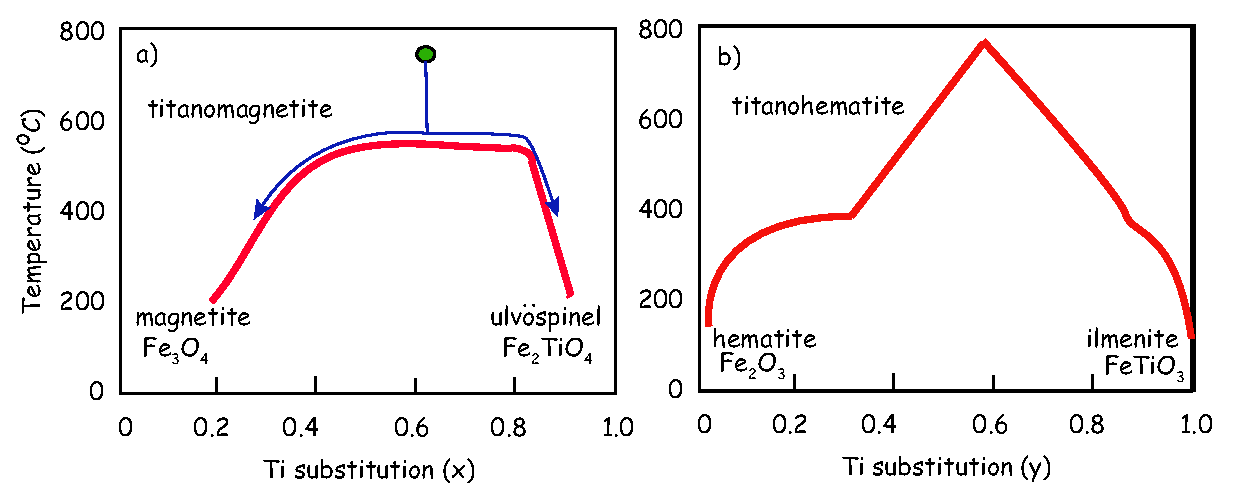
\includegraphics[width=13 cm]{EPSfiles/solidsolution.eps}
\caption{Phase diagrams for FeTi oxides.  The composition is indicated by $x$ or $y$. 
There is complete solid solution above the solid lines.  Exolution begins as the temperature cools below the solid curves.  a) Titanomagnetite series. [Redrawn from Nagata, 1961.] b) Titanohematite series.  [Redrawn from Robinson et al. 2004.]}
\label{fig:solidsolution}
\end{figure}
 \nocite{robinson04} \nocite{nagata61}


\index{exsolution} 
 Exsolution is important in paleomagnetism for two reasons.  First, the different compositions have very different magnetic properties.  Second,  the lamellae effectively reduce the magnetic crystal size which we already know has a profound influence on the magnetic stability of the mineral.   An example of this is shown in Figure~\ref{fig:exsolution}b in which the larger crystal is  several microns in width, too large to have single domain-like magnetization, yet the smaller magnetite lamellae are indeed small enough and carry a strong stable magnetization 
 \index{Feinberg, J.M.}
 (Feinberg et al. 2005). \nocite{feinberg05}


\begin{figure}[htb]
%\epsfxsize 12cm
%\centering \epsffile{EPSfiles/exsolution.eps}
\centering  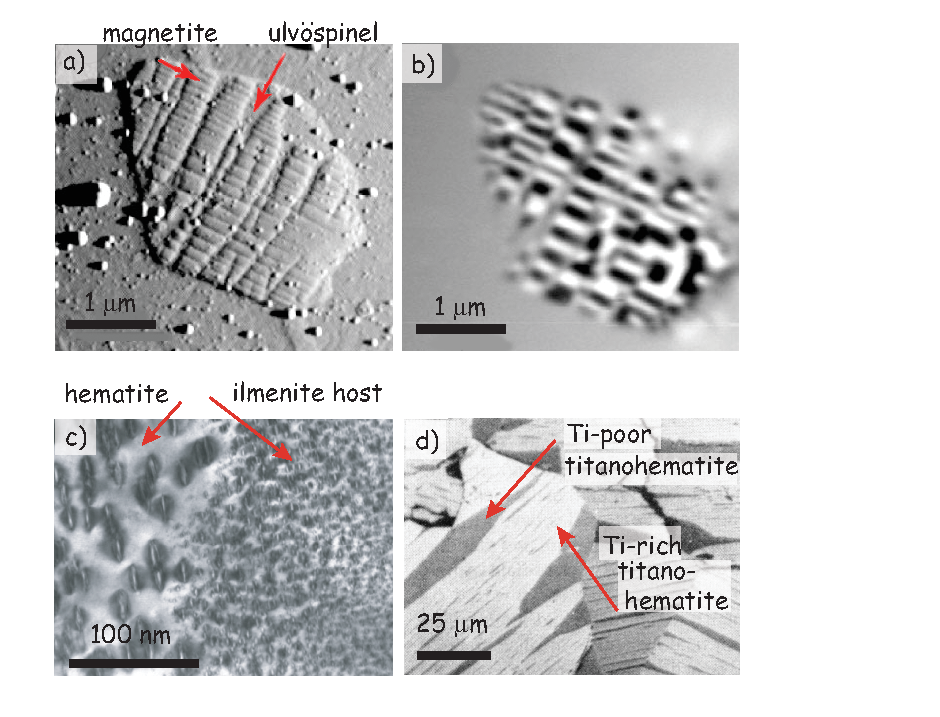
\includegraphics[width=12 cm]{EPSfiles/exsolution.eps}
\caption{a) Atomic force micrograph image of magnetite inclusion in clinopyroxene.  The topographically low areas are ulv\"ospinel while the higher areas are magnetite.  b) Magnetic force micrograph of magnetic domains (black and white are oppositely magnetized).  The ulv\"ospinel lamellae are essentially non-magnetic and are gray    c) Tranmission electron micrograph of ilmenite host with hematite exolution lamellae.  Lamellar size gets smaller  with proximity to edge.   d) Photomicrograph of  titanohematite exolution lamellae. Dark bands are Ti-rich (high  magnetization, low $T_c$), light grey bands are Ti-poor (low magnetization, high $T_c$).  [a and b are from Feinberg et al., 2005, c) from Robinson et al., 2002., d) is modified from S. Haggerty in Butler (1992).]}
\label{fig:exsolution}
\end{figure}
\nocite{feinberg05,robinson02,butler92}

 
 
\begin{figure}[htb]
%\epsfysize 3in
 %\centering \epsffile {EPSfiles/tern.eps}
\centering  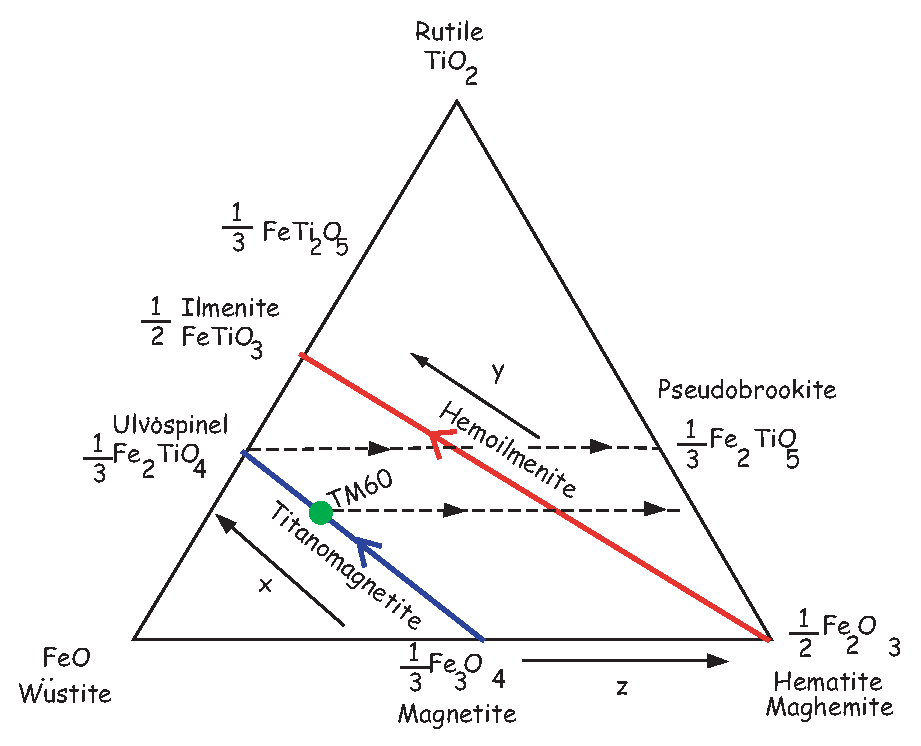
\includegraphics[width=3 in]{EPSfiles/tern.eps}
\caption{Ternary diagram for iron-oxides.
The solid lines are solid solution series with increasing titanium concentration ($x$). 
The dashed lines with arrows indicate the direction of increasing
oxidation ($z$). [Figure redrawn from  Butler, 1992.] }
\label{fig:tern}
\end{figure}
 \nocite{oreilly84}

Compositions of minerals are frequently plotted on 
\index{diagrams!ernary}
ternary diagrams like the one shown in Figure~\ref{fig:tern}.  [For help in reading ternary diagrams, please see the Appendix~\ref{app:ternary}]  
The apices of the ternary diagram are Fe$^{2+}$ on the lower left, Fe$^{3+}$ on the lower right and Ti$^{4+}$ on the top.   The oxides with these species are FeO (w\"ustite),  Fe$_2$O$_3$ (hematite or maghemite depending on structure) and TiO (rutile).  Every point on the triangle represents a cation mixture or solution that adds up to one cation (hence the fractional formulae).  

Each of the solid arrows in Figure~\ref{fig:tern} (labelled titanomagnetite and hemoilmenite) represent
increasing substitution of titanium into the crystal lattices of magnetite and
hematite respectively.
  The amount of Ti substitution in
titanomagnetites is denoted by ``$x$'', while substitution in the
hemoilmenites is denoted by ``y''.
Values for $x$ and $y$  range from 0 (magnetite or hematite) to 1 
(ulv\"ospinel or ilmenite).    






\subsection {Titanomagnetites Fe$_{3-x}$Ti$_x$O$_4$} 
\label{sect:titano}

\index{magnetite}%
\index{inverse spinel}%
\index{titanomagnetite}
In earlier chapters on rock magnetism, we learned a few things about magnetite.  As mentioned in Chapter 4, magnetite (Fe$_3$O$_4$) has an
inverse spinel structure (AB$_2$O$_4$).  The oxygen atoms form a face-centered cubic
lattice into which cations fit in either octahedral or tetrahedral symmetry. 
 For each
unit cell there are four tetrahedral sites (A) and eight octahedral sites (B). 
To maintain charge balance with the four oxygen ions (O$^{2-}$), 
there are two Fe$^{3+}$ ions
and one Fe$^{2+}$ ion. 
Fe$^{3+}$ has five unpaired spins, while Fe$^{2+}$ has four.  As
discussed in Chapter  3, each unpaired spin contributes a moment of one 
\index{Bohr magneton}% 
Bohr magneton ($m_b$). 
The divalent iron ions all reside in the octahedral lattice
sites, whereas  the trivalent iron ions are split evenly between octahedral and
tetrahedral sites: Fe$^{3+}|$Fe$^{3+}$Fe$^{2+}|$O$_4$.  The A and B lattice sites are
coupled with antiparallel spins and magnetite is ferrimagnetic.
Therefore, the net moment of  magnetite is (9-5=4)  $m_b $ per molecule
(at 0 K).

 \begin{figure}[htb]
%\epsfxsize 14cm
%\centering \epsffile{EPSfiles/X.eps}
\centering  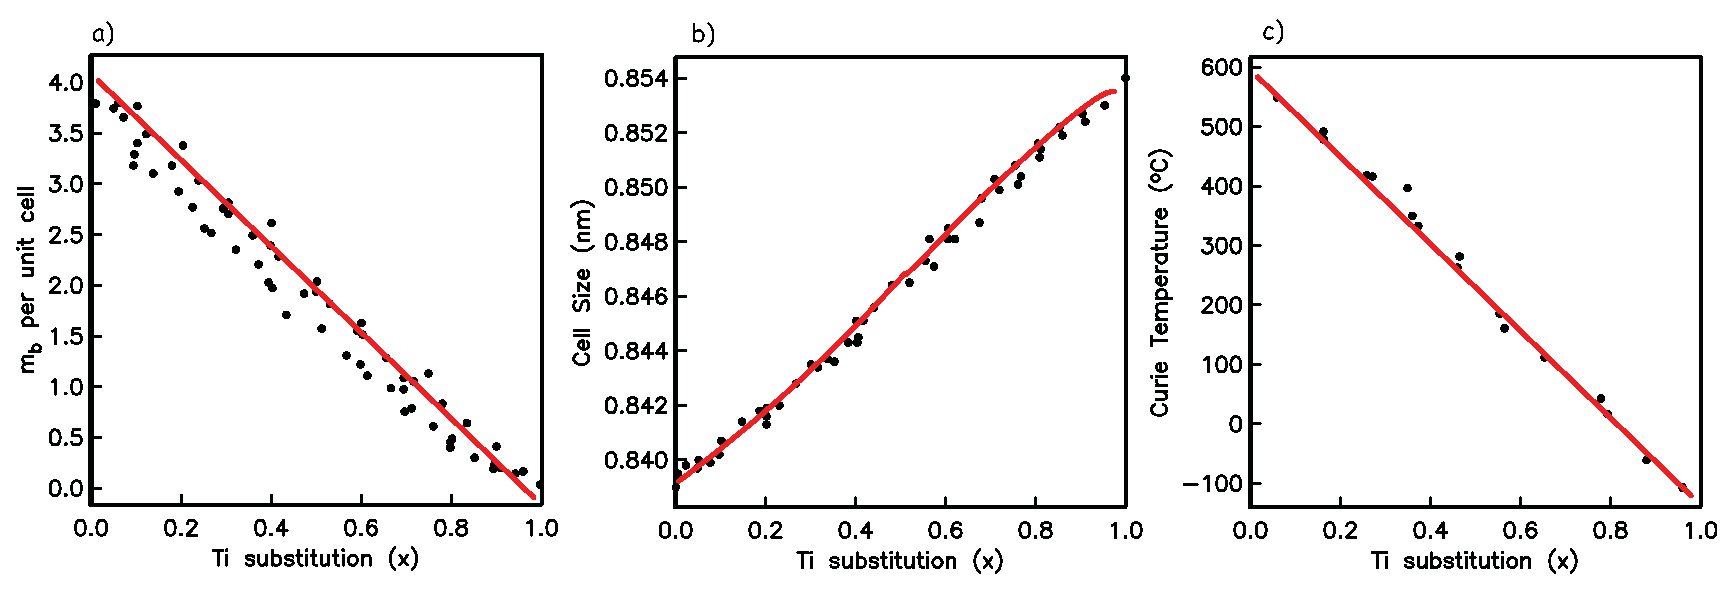
\includegraphics[width=14 cm]{EPSfiles/X.eps}
\caption{Variation of intrinsic parameters with titanium substitution in the titanomagnetite lattice.  X is the degree of substitution from 0 (no Ti) to 1 (100\% substitution).  a) Variation of the magnetization expressed as Bohr magnetons per unit cell.  b) Variation of cell lattice size.  c) Variation of Curie temperature. [Data compiled by O'Reilly, 1984.])}
\label{fig:X}
\end{figure} \nocite{oreilly84}


Titanomagnetites can occur 
as  primary minerals in igneous rocks.  Magnetite, as well as various
members of the hemoilmenite series, can also form as a
result of high temperature 
oxidation.  In sediments, magnetite often occurs as a 
detrital component.  It can
also be produced by bacteria or authigenically during diagenesis.

Substitution of Ti$^{4+}$, which has no unpaired spins (see Chapter 3),
 has a profound effect on the magnetic properties of the
resulting titanomagnetite.  Ti$^{4+}$ substitutes for a trivalent iron ion.
In order to maintain charge balance, another trivalent iron ion turns into a divalent iron
ion.  The end members of the solid solution series are:

\begin{center}
\begin{tabular}{cc}
\hline
 magnetite  &  ulv\"ospinel \\
 Fe$^{3+}|$Fe$^{3+}$Fe$^{2+}|$O$_4$  &  Fe$^{2+}|$Fe$^{2+}$Ti$^{4+}|$O$_4$ \\
 $x = 0 $ &  $x=1$  \\
\hline
\end{tabular}
\end{center}

\begin{figure}[htb]
%\epsfxsize 14cm
%\centering \epsffile{EPSfiles/hematite.eps}
\centering  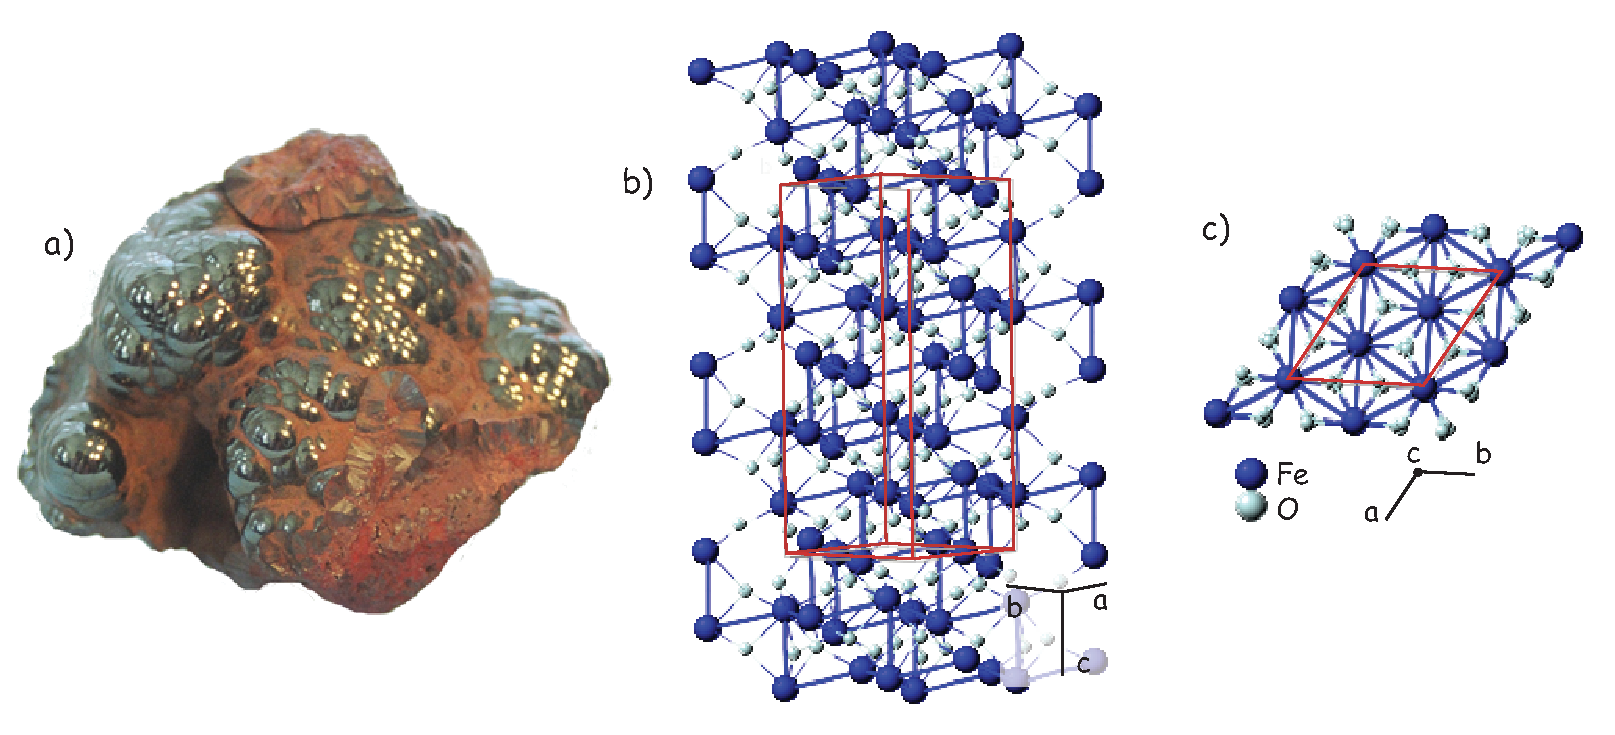
\includegraphics[width=14 cm]{EPSfiles/hematite.eps}
\caption{Hematite. a) Photograph of Kidney ore hematite from Michigan by DanielCD. [From commons.wikimedia.org/wiki/File:Hematite.jpg.]   b-c) Two views of the crystal structure of hematite.  c-axis is perpendicular to the basal plane. [From \url{http://www.webmineral.com}.] }
\label{fig:hematite}
\end{figure} 


\index{antiferromagnetism}%
\index{ulv\"ospinel}%
Ulv\" ospinel is antiferromagnetic because the A and B lattice sites have the
same net moment.  When $x$ is between 0 and 1, the mineral is called a
titanomagnetite.  If $x$ is 0.6,  for example, the mineral
is called TM60 (green dot in Figure~\ref{fig:tern}).  

\index{titanium substitution}%
The profound effect of titanium substitution on the intrinsic properties of titanomagnetite is illustrated in Figure~\ref{fig:X}.  Because Ti$^{4+}$ has no unpaired spins, the saturation magnetization decreases with increasing $x$ (Figure~\ref{fig:X}a).   The cell dimensions increase with increasing $x$ (Figure~\ref{fig:X}b).  As a result of the increased cell dimension, there is a decrease in
\index{Curie temperature}
 Curie Temperature (Figure~\ref{fig:X}c).  There is also a    slight increase in  coercivity (not shown).  

The large $M_s$ of magnetite (see Table~\ref{tab:rockpars}) means that
for deviations from equant grains as small as 10\%, 
\index{magnetic!anisotropy energy}%
the magnetic anisotropy energy becomes dominated by shape. 
Nonetheless, aspects of the
\index{magnetic!anisotropy!energy!magnetocrystalline}%
magnetocrystalline anisotropy provide useful diagnostic tests.  The
magnetocrystalline anisotropy constants are a strong function of
temperature. On warming to $\sim$-100$^{\circ}$C from
near absolute zero, changes in
these constants can lead to an abrupt loss of magnetization, which is
known loosely as the 
\index{Verwey transition}%
{\it Verwey transition} (see Chapter 4).  Identification of the Verwey
transition suggests a remanence that is dominated by magnetocrystalline
anisotropy.  As we shall see, 
the temperature at which it occurs is sensitive to oxidation and the
transition can be
completely supressed by maghemitization (see 
Dunlop and \"Ozdemir [1997]). 

It should be noted that natural titanomagnetites often contain impurities (usually Al, Mg, Cr).  These impurities also affect the magnetic properties.   Substitution of 0.1 Al$^{3+}$ into the unit cell of titanomagnetite results in a 25\% reduction in $M_s$ and a reduction of the Curie temperature by some 50$^{\circ}$C.  Substitution of Mg$^{2+}$ into TM60 also results in a lower saturation magnetization with a reduction of some 15\%. 

\begin{figure}
%\epsfxsize 14cm
%\centering \epsffile{EPSfiles/hemY.eps}
\centering  \includegraphics[width=14 cm]{EPSfiles/hemY.eps}
\caption{Variation of properties with Ti substitution in the titanohematite series.  a) Variation of saturation magnetization.  b) Variation of N\'eel Temperature.  [Modified from Nagata, 1961 and Stacey and Banerjee, 1974.]}
\label{fig:hemY}
\end{figure}
\nocite{nagata61,stacey74}



\subsection {Hematite-Ilmenite Fe$_{2-y}$Ti$_y$O$_3$}
\label{sect:hemo}

\index{hematite}%
Hematite has a corundum  structure (see Figure~\ref{fig:hematite}).  It is rhombohedral with a pseudocleavage
(perpendicular to the $c$ axis) and  tends to break into flakes.  
It is
antiferromagnetic, with a weak 
parasitic ferromagnetism  resulting from either 
spin-canting or 
defect ferromagnetism (see Chapter 3).
 Because the magnetization is a spin canted antiferromagnetism, the temperature at which this magnetization disappears is called the 
 \index{N\'eel!temperature}
 N\'eel Temperature instead of the Curie Temperature which is {\it sensu strictu} only for ferromagnetic minerals.  
The N\'eel temperature for hematite is approximately 685$^{\circ}$C.  


  Above about -10$^{\circ}$C (the 
\index{Morin transition}%
{\it Morin
transition}), the magnetization is constrained by aspects of the crystal
structure to lie
perpendicular to the $c$ axis or within the basal plane.  Below the Morin transition, 
\index{spin-canting}
spin-canting all but disappears
and the magnetization is parallel to the $c$ axis.  This effect could be used to
demagnetize the grains dominated by spin-canting: it 
does not affect those dominated by defect
moments.   Most hematites  formed at  low-temperatures have magnetizations dominated by defect moments, so the remanence of many rocks will not display a Morin transition.


 \begin{figure}[h!tb]
%\epsfxsize 14cm
%\centering \epsffile{EPSfiles/Z.eps}
\centering  \includegraphics[width=14 cm]{EPSfiles/Z.eps}
\caption{Variation of intrinsic parameters with oxidation in TM60.  $z$ is the degree of oxidation.  a) Variation of the magnetization.   b) Variation of cell lattice size.  c) Variation of Curie temperature. [Data compiled by Dunlop and \"Ozdemir, 1997.]  inset: A magnetite crystal ($\sim$ 30 $\mu$m) undergoing maghemitization.  Because of the change in volume, the crystal begins to crack. [From Gapeyev and Tsel'movich, 1988 in Dunlop and \"Ozdemir, 1997.]}
\label{fig:Z}
\end{figure}\nocite{gapeyev88}


Hematite occurs widely in oxidized sediments and dominates the magnetic
properties of red beds.  It occurs as a high temperature oxidation product 
in certain igneous rocks.  Depending on grain size, among
other things, it is either
black (specularite) or red (pigmentary).  Diagnostic properties of hematite are listed in Table~\ref{tab:rockpars}.



The substitution of Ti into the lattice structure of $\alpha$Fe$_2$O$_3$ has an even more profound influence on magnetic properties  than for magnetite.  For $y=0$ the magnetization is spin-canted antiferromagnetic, but when $y=0.45$, the magnetization becomes ferrimagnetic (see Figure~\ref{fig:hemY}a).   For small amounts of substitution, the Ti and Fe cations are distributed equally among the cation layers.  For $y>0.45$, however, the Ti cations preferentially occupy alternate cation layers.  Remembering that the Ti$^{4+}$  ions have no net moment, we can imagine  that antiparallel coupling between the two sub-lattices results in ferrimagnetic behavior, as opposed to the equal and opposite style of anti-ferromagnetism.  



\index{titanohematite}
Titanohematite particles with intermediate values of $y$ have interesting properties from a paleomagnetic point of view.   There is a solid solution at high temperatures, but as the temperatures drop the crystals exsolve into titanium rich  and poor  lamellae (see Figure~\ref{fig:exsolution}d).  Figure~\ref{fig:hemY} shows the variation in saturation magnetization and N\'eel  temperature with Ti substitution.   For certain initial liquid compositions, the exolution lamellae could have Ti-rich bands alternating with Ti-poor bands.  If the Ti-rich bands have higher magnetizations, yet lower Curie temperatures than the Ti-poor bands, the Ti-poor bands will become magnetized first.  When the Curie temperature of the Ti-rich bands is reached, they will become magnetized in the presence of the demagnetizing field of the Ti-poor bands, hence they will acquire a remanence that is antiparallel to the applied field.  Because these bands have higher magnetizations, the net NRM will also be anti-parallel to the applied field and the rock will be {\it self-reversed}.   This is fortunately very rare in nature.


 \begin{figure}[htb]
%\epsfxsize 11cm
%\centering \epsffile{EPSfiles/suppress.eps}
\centering  \includegraphics[width=11 cm]{EPSfiles/suppress.eps}
\caption{Effect of maghemitization on Verwey transition.  a) Saturation remanence acquired at 10 K observed as it warms up for 37 nm stoichiometric magnetite.  b) Same but for partially oxidized magnetite. [Data from \"Ozdemir et al., 1993.]  }
\label{fig:suppress}
\end{figure}
\nocite{ozdemir93}


\subsection {Oxidation of (titano)magnetites to (titano)maghemites}

Many minerals form under one set of equilibrium conditions (say within a cooling lava flow) and are later subjected to a different set of conditions (sea-floor alteration or surface weathering).  They will tend to alter in order to come into equilibrium with the new set of conditions.   The new conditions are often more oxidizing than the original conditions and compositions tend to move along the dashed lines in Figure~\ref{fig:tern}.    The degree of oxidation is represented by the parameter $z$. 

While the solid solution between magnetite and ulv\"ospinel exists in principle, intergrowths of these two minerals are actually quite rare in nature because the titanomagnetites interact with oxygen in the melt to form intergrowths of low Ti magnetite with ilmenite.  This form of oxidation is known as 
\index{deuteric oxidation}
{\it deuteric} oxidation.  


 

Low temperature oxidation will tend to transform a single phase spinel (titanomagnetite) into a new single phase spinel (titanomaghemite) by diffusion of  Fe$^{2+}$ from the lattice structure of the (titano)magnetite to the surface where it is converted to Fe$^{3+}$;  
\index{titanomaghemite}
titanomaghemite   is a ``cation-deficient''  inverse  spinel.     The inset to  Figure~\ref{fig:Z}c shows a magnetite crystal in the process of becoming maghemite.  The conversion of the Fe$^{2+}$ ion means a loss in volume which results in characteristic cracking of the surface.   There is also a loss in magnetization, a shrinkage of cell size and, along with the tightening unit cell, an increase in Curie Temperature.  These trends are shown for TM60 in Figure~\ref{fig:Z}.  Maghematization results in a much reduced Verwey transition (see Figure~\ref{fig:suppress}).  


 


 The (titano)maghemite  structure is metastable and can invert to form the isochemical, but more stable structure of (titano)hematite, or it can be reduced to form magnetite.    The two forms of Fe$_2$O$_3$ are distinguished by the symbols $\gamma$ for maghemite and $\alpha$ for hematite.    Inversion of natural maghemite is usually complete by about 350$^{\circ}$C,
but it can survive until much higher temperatures (for more details, see
\index{Dunlop, D.J.}
\index{\"Ozdemir, \"O.}
\nocite{dunlop97}
 Dunlop and \"Ozdemir, 1997).     Also, it is common that the outer rim of the magnetite will be oxidized to maghemite, while the inner core remains magnetite.    


 
\begin{figure}[htb]
%\epsfxsize 14cm
%\centering \epsffile{EPSfiles/minerals.eps}
\centering  \includegraphics[width=14 cm]{EPSfiles/minerals.eps}
\caption{  a) Photograph of goethite. [From  en.wikipedia.org/wiki/Image:Goethite3.jpg; photo of  Eurico Zimbres.]   b) Goethite crystal structure. 
c) Photograph of greigite.  [Photo of William P\'eraud.]   d) Greigite crystal structure. 
e) Photograph of single crystal of pyrrhotite. [Photo of Dan Weinrich.]  f) Pyrrhotite crystal structure.  [All crystal structure images from \url{http://www.webminerals.com}.]}
\label{fig:minerals}
\end{figure}


\section {Iron-oxyhydroxides and iron-sulfides}
\label{sect:pyrrho}

\index{iron-oxyhydroxides}%
Of the many  iron oxyhydroxides that occur in any abundance
in nature, 
\index{goethite}%
goethite ($\alpha$FeOOH; Figure~\ref{fig:minerals}a,b) is the most common magnetic phase. It is
\index{antiferromagnetism}%
\index{defect ferromagnetism}%
antiferromagnetic with what is 
most likely a defect magnetization.  It occurs
widely as a weathering product of iron-bearing minerals and as a direct
precipitate from iron-bearing solutions.  It is metastable  under
many conditions and dehydrates to
hematite with time or elevated temperature.  Dehydration is usually complete by
about 325$^{\circ}$C.  It is characterized by a very high coercivity but a low 
\index{N\'eel!temperature}
N\'eel
temperature of about 100--150$^{\circ}$C.
 Diagnostic properties of goethite are listed in Table~\ref{tab:rockpars}.
 


There are two 
\index{iron-sulfides}%
iron-sulfides that are important to paleomagnetism: 
\index{greigite}%
greigite (Fe$_3$S$_4$; Figure~\ref{fig:minerals}c,d) and
\index{pyrrhotite}%
pyrrhotite (Fe$_7$S$_8$-Fe$_{11}$S$_{12}$; Figure~\ref{fig:minerals}e,f).  These are ferrimagnetic and occur in reducing environments.  They 
both  tend to oxidize to various iron oxides leaving paramagnetic 
\index{pyrite}%
pyrite as the
sulfide component.  


The Curie temperature of 
\index{pyrrhotite!monoclinic}
monoclinic pyrrhotite (Fe$_7$S$_8$)
is about 325$^{\circ}$C (see Figure~\ref{fig:pyrrhotiteT}b; Table~\ref{tab:rockpars}). Monoclinic pyrrhotite undergoes a transition 
at $\sim$ 35 K, so low temperature measurements can be diagnostic for this phase (see Figure~\ref{fig:pyrrhotiteT}a).   
\index{pyrrhotite!hexagonal}
Hexagonal pyrrhotite undergoes a structural transition from an imperfect antiferromagnet to a ferromagnet with much higher saturation magnetization at about 200$^{\circ}$C.  During a thermomagnetic experiment, the expansion of the crystal results in a large peak  in magnetization just below the Curie Temperature (see Figure~\ref{fig:pyrrhotiteT}c).    Mixtures of monoclinic and hexagonal pyrrhotite result in the behavior sketched in Figure~\ref{fig:pyrrhotiteT}d.   
The maximum unblocking temperature of
\index{greigite}
 greigite is approximately
330$^{\circ}$C. 
 Other diagnostic properties of greigite and pyrrhotite are listed in 
Table~\ref{tab:rockpars}.




\begin{figure}[htb]
\centering
%\epsfxsize 14cm
% \epsffile{EPSfiles/pyrrhotiteT.eps}
 \includegraphics[width=13 cm]{EPSfiles/pyrrhotiteT.eps}
\caption{a) Low-temperature transition in monoclinic pyrhotite. [Data from Snowball and Torrii, 1999.]
 Thermomagnetic curves for b) monoclinic c) hexagonal and d) mixture of b) and c) pyrrhotite.  [Data from Dekkers, 1988.]}
\label{fig:pyrrhotiteT}
\end{figure}
\nocite{dekkers88}


\nocite{snowball99}





\section{FeTi oxides in igneous rocks}

The composition and relative proportions of FeTi oxides, crystallizing from a silicate melt depend on a number of factors, including the bulk chemistry of the melt, oxygen fugacity and the cooling rate. The final assemblage may be altered after cooling.  FeTi oxides are generally more abundant in mafic volcanic rocks (e.g. basalts) than silicic lavas (e.g., rhyolites).  FeTi oxides can be among the first liquidus phases ($\sim$ 1000$^{\circ}$C) in silicic melts, but in mafic lavas they generally are among the last phases to form ($\sim$1050$^{\circ}$C), often with plagioclase and pyroxene.  

Although there is considerable variability, the Ti (ulv\"ospinel) content of the titanomagnetite crystallizing from a melt generally is lower in more silicic melts (see solid black lines in Figure~\ref{fig:igneous}).   Titanomagnetites in tholeiitic lavas generally have 0.5 $<x<$ 0.8 with an initial composition near TM60 ($x$=0.6) characteristic for much of the oceanic crust.  The range of rhombohedral phases (dashed red lines)  crystallizing from silicate melts is more limited, $0.05<y<0.3$ for most lavas.   




\begin{figure}[htb]
%\centering \epsffile{EPSfiles/igneous.eps}
\includegraphics[width=13 cm]{EPSfiles/igneous.eps}
\caption{Occurrence of FeTi oxides in igneous rocks.  [Data from Frost and Lindsley, 1991.]}
\label{fig:igneous}
\end{figure}\nocite{frost91}


The final magnetic mineral assemblage in a rock is often strongly influenced by the cooling rate and oxygen fugacity during initial crystallization.  As a first approximation, we distinguish slowly cooled rocks (which may undergo solid state exsolution and/or deuteric oxidation) from those in which the oxide minerals were rapidly quenched.  As mentioned before, FeTi oxides in slowly cooled igneous rocks can exhibit exolution lamellae with bands of low and high titanium magnetites if the oxygen fugacity remains unoxidizing.   This reaction is very slow, so its effects are rarely seen in nature. 

The typical case in slowly cooled rocks is that the system becomes more oxidizing with increasing differentiation during cooling and crystallization.  For example, both the dissociation of magmatic water and the crystallization of silicate phases rich in Fe will act to increase the oxidation state.  This will drive compositions to higher $z$ values (see Figure~\ref{fig:tern}).  The final assemblage typically consists of ilmenite lamellae and a nearly pure magnetite host because adding $O_2$ drives the reaction 
$
Fe_2TiO_4 + O_2 \rightleftharpoons Fe_3O_4$
to the right.  This process is known as {\it oxyexsolution}.  Under even more oxidizing conditions, these phases may ultimately be replaced by their more oxidized counterparts (e.g., hematite, pseudobrookite).  

Weathering at ambient surface conditions or mild hydrothermal alteration may lead to the development of cation deficient (titano)maghemites.  This can either occur by addition of oxygen to the spinel phase with a corresponding oxidation of the Fe$^{2+}$ to Fe$^{3+}$ to maintain charge balance, or by the removal of some of the octahedral iron from the crystal structure.  


\begin{figure}[htb]
%\epsfxsize 14cm
%\centering \epsffile{EPSfiles/bacteria.eps}
\includegraphics[width=13 cm]{EPSfiles/bacteria.eps}
\caption{Photomicrographs of bacterial magnetites produced by magnetotactic bacteria.  a) Intact magnetosome in living bacterium. [False color image from H. Vali in Maher and Thompson, 1999.]  b) Chains recovered from ODP Site 1006D in the Bahamas [From M. Hounslow in Maher and Thompson, 1999.]}
\label{fig:bacteria}
\end{figure}
\nocite{maher99}
%\nocite{fassbinder90}



\section{Magnetic mineralogy of soils and sediments}

Igneous (and metamorphic) rocks are the ultimate source for the components of sedimentary rocks, but biological and low-temperature diagenetic agents work to modify these components and have a significant effect on magnetic mineralogy in sediments.  As a result there is a virtual rainbow of magnetic mineralogies found in sediments.     (Titano)magnetite coming into the sedimentary environment from an igneous source may experience a change in pH and redox conditions that make it no longer the stable phase, hence it may alter.   
Also,   although the geochemistry of seawater is generally oxidizing with respect to the stability field of magnetite, pronounced changes in the redox state of sediments often occur with increasing depth as a function of the breakdown of organic carbon.  Such changes may result in locally strongly reducing environments where magnetite may be dissolved and authigenic sulfides produced.  Indeed,  changes down sediment cores  in the ferrimagnetic mineral content and porewater geochemistry suggest that this process is active in some (most?) marine sedimentary sequences. For example, dissolution of magnetite and/or production of non-magnetic sulfides may be responsible for the oft-seen decrease in various bulk magnetic parameters (e.g., magnetic susceptibility, IRM, ARM, etc.) with depth.   




Some of the more spectacular magnetic minerals found in sediments are biogenic magnetites produced by magnetotactic bacteria (see recent review by Kopp and Kirsch- vink, 2008 and Figure~\ref{fig:bacteria}).   The sizes and shapes of
\index{magnetite!bacterial}
 bacterial magnetite, when plotted on the 
\index{diagrams!Evans}
 Evans diagram from Chapter 4, suggest that magnetotactic bacteria form magnetite in the single domain grain size range -- otherwise extremely rare in nature.    It appears that  bacterial magnetites are common in sediments, but their role in contributing to the  natural remanence is still poorly understood. 



 \nocite{oreilly84,dunlop97}
 \nocite{snowball90}\nocite{dekkers88}\nocite{dekkers89}\nocite{dekkers89b} \nocite{ozdemir93}\nocite{banerjee71}\nocite{worm93}\nocite{collinson83}\nocite{rochette90}\nocite{spender72}\nocite{snowball90}\nocite{roberts95}
\nocite{dunlop97}\nocite{dekkers89c}
 \begin{center}
\begin{longtable}{ll}
\caption [Physical properties of magnetic minerals.] {Physical properties of magnetic minerals.}
\label{tab:rockpars}\\

\hline
{Magnetite:}&Fe$_3$O$_4$\\
\endfirsthead

\multicolumn{2}{l}%
{\tablename\ \it  -- continued from previous page} \\
\hline
\endhead

\hline \multicolumn{2}{r}{{\it Continued on next page --}} \\
\endfoot
\hline
\endlastfoot

Density = 5197 kg m$^{-3}$& Dunlop and \"Ozdemir [1997]\\
{Curie temperature}  = 580$^{\circ}$C & Dunlop and \"Ozdemir [1997]\\
{Saturation Magnetization}  = 92 Am$^2$kg$^{-1}$&O'Reilly [1984]\\
{Anisotropy Constant} = -2.6 {Jkg}$^{-1}$&  Dunlop and \"Ozdemir [1997]\\
{Volume susceptibility} = $\sim$ 1 SI& O'Reilly [1984]\\
 {Typical coercivities are 10's of mT}& O'Reilly [1984] \\
 Verwey transition: 110-120 K& \" Ozdemir and Dunlop [1993]\\
Cell edge = 0.8396 nm & Dunlop and \"Ozdemir [1997]\\
\hline
Maghemite:&$\gamma$Fe$_2$O$_3$\\
Density = 5074 kg m$^{-3}$& Dunlop and \"Ozdemir [1997]\\
{Curie temperature}  = 590-675$^{\circ}$C & Dunlop and \"Ozdemir [1997]\\
{Saturation Magnetization}  = 74 Am$^2$kg$^{-1}$& Dunlop and \"Ozdemir
[1997]\\
{Anisotropy Constant} = 0.92 {Jkg}$^{-1}$&  Dunlop and \"Ozdemir [1997]\\
 Verwey transition: suppressed& Dunlop and \"Ozdemir [1997]\\ 
Breaks down to $\alpha$Fe$_2$O$_3$: between 250$\rightarrow$ 
750$^{\circ}$C &
Dunlop and \"Ozdemir [1997]\\
\hline
TM60:&Fe$_{2.4}$Ti$_{0.6}$O$_4$\\
Density = 4939 kg m$^{-3}$& Dunlop and \"Ozdemir [1997]\\
{Curie temperature}  = 150$^{\circ}$C & Dunlop and \"Ozdemir [1997]\\
{Saturation Magnetization}  = 24 Am$^2$kg$^{-1}$& Dunlop and \"Ozdemir
[1997]\\
{Anisotropy Constant} = 0.41 {Jkg}$^{-1}$&  Dunlop and \"Ozdemir [1997]\\
 {Coercivity $\sim$ 8 mT}& Dunlop and \"Ozdemir [1997]\\
Verwey transition: suppressed&Dunlop and \"Ozdemir [1997]\\
Cell edge = 0.8482 nm &Dunlop and \"Ozdemir [1997]\\
\hline
{Hematite:}&$\alpha$Fe$_2$O$_3$\\
Density = 5271 kg m$^{-3}$& Dunlop and \"Ozdemir [1997]\\
{N\' eel temperature} = 675$^{\circ}$C&O'Reilly [1984]\\
{Saturation Magnetization} = 0.4 Am$^2$kg$^{-1}$&O'Reilly [1984]\\
{Anisotropy Constant }  = 228 {Jkg}$^{-1}$&Dunlop and \"Ozdemir [1997]\\
{Volume susceptibility} = $\sim$ 1.3 x 10$^{-3}$ SI& O'Reilly [1984]\\
 {Coercivities vary widely and can be 10's of teslas}& 
Banerjee [1971]\\
Morin Transition: $\sim$ 250-260 K (for $>$ 0.2 $\mu$m)&O'Reilly [1984]\\
{Goethite:} & $\alpha$FeOOH\\
Density = 4264 kg m$^{-3}$& Dunlop and \"Ozdemir [1997]\\
{N\' eel temperature}: 70 $\rightarrow$ 125$^{\circ}$C & O'Reilly [1984]\\
{Saturation Magnetization} = 10$^{-3}\rightarrow$ 1 Am$^2$kg$^{-1}$ & O'Reilly [1984]\\
{Anisotropy Constant}  = 0.25 $\rightarrow $ 2 {Jkg}$^{-1}$&Dekkers [1989]\\
{Volume susceptibility} = $\sim$ 1 x 10$^{-3}$ SI& Dekkers [1989a]\\
 {Coercivities can be 10's of teslas}\\
Breaks down to hematite: 250 $\rightarrow$ 400$^{\circ}$C\\
\hline
{Pyrrhotite:} &Fe$_7$S$_8$\\
Density = 4662 kg m$^{-3}$& Dunlop and \"Ozdemir [1997]\\
Monoclinic:\\
{Curie temperature } = $\sim$ 325$^{\circ}$C&Dekkers [1989]\\
Hexagonal:\\
{Curie temperature } = $\sim$270$^{\circ}$C&Dekkers [1988]\\
{Saturation Magnetization} = 0.4 -$\sim$ 20 Am$^2$kg$^{-1}$&Worm et al. [1993]\\
{Volume susceptibility} = $\sim$ 1 x 10$^{-3}\rightarrow 1$ SI& Collinson [1983];O'Reilly [1984]\\
{Anisotropy Constant}  = 20 {Jkg}$^{-1}$&O'Reilly [1984]\\
 {Coercivities vary widely and can be 100's of mT}&O'Reilly [1984]\\
Has a transition at $\sim$ 34  K &Dekkers et al. [1989]\\
&Rochette et al. [1990] \\
Hexagonal pyrrotite:  transition near 200$^{\circ}$\\
Breaks down to magnetite: $\sim$ 500$^{\circ}$C&Dunlop and \"Ozdemir
[1997]\\
\hline
{Greigite:}&Fe$_3$S$_4$\\
Density = 4079 kg m$^{-3}$& Dunlop and \"Ozdemir [1997]\\
Maximum unblocking temperature = $\sim$ 330$^{\circ}$C&Roberts [1995]\\
{Saturation Magnetization} = $\sim$ 25 Am$^2$kg$^{-1}$&Spender et al. [1972]\\
{Anisotropy Constant}  = -0.25 {Jkg}$^{-1}$&Dunlop and \"Ozdemir
[1997]\\
{Coercivity 60$\rightarrow >$ 100 mT}& Roberts [1995]\\
Has high $M_r/\chi$ ratios $\sim$ 70 x 10$^3$ Am$^{-1}$& Snowball and Thompson
[1990]\\ 
{Breaks down to magnetite:}
 $\sim$ 270-350$^{\circ}$C&Roberts [1995]\\
\end{longtable}
\end{center}

\noindent{SUPPLEMENTAL READINGS:} Dunlop and \"Ozdemir (1997), Chapter 3;  
 Kopp and Kirschvink (2008). \nocite{kopp08}


\begin{figure}[htb]
%\epsfxsize 3in
%\centering \epsffile{EPSfiles/problem1.eps}
\includegraphics[width=3 cm]{EPSfiles/problem1.eps}
\caption{Curie Temperature curves for two samples, A and B. [Figure redrawn from Butler, 1992.]}
\label{fig:prob1}
\end{figure}

\clearpage

\nocite{butler92}
\section{Problems}




{{\parindent 0pt \parskip 12pt 

{\bf Problem 1}

You measured Curie Temperature curves for two samples A and B as shown in Figure~\ref{fig:prob1}.  Based on your knowledge of Curie Temperatures,  what is the likely magnetic mineralogy for each sample?  



{\bf Problem 2}

The data in {\it demag.dat} in the Chapter\_6 data directory (see Problems for  Chapter 5 for downloading instructions) are thermal demagnetization data for a 
specimen that had a 2 T field exposed along $x$, a 0.4 T field
exposed along $y$ and a 0.12 T field exposed along $z$.    The sample was then heated to a particular temperature
step ($^{\circ}$C) and cooled in zero magnetic field, allowing all grains that become superparamagnetic at temperatures lower than the treatment temperature to become randomized.  After each treatment step, the magnetic vector was measured.    The column headings are:  Treatment temperature (C), Intensity, Declination, Inclination.  


a) Write a python program to read the data in and convert the declination, inclination and intensity to cartesian components.  

b) Modify your program to normalize the intensity to the 20$^{\circ}$C  measurement. 

c)  Extend the program to plot  the $x$ and $y$ components as a function of temperature.   

d)  Based on your understanding of coercivity and Curie temperatures, what is carrying the $x$ and $y$ components?  

\begin{figure}[h!tb]
%\epsfxsize 12cm
%\centering \epsffile{EPSfiles/microprobe.eps}
\includegraphics[width=13 cm]{EPSfiles/microprobe.eps}
\caption{a) Thermomagnetic run of mineral whereby magnetization (normalized by the initial value) is measured as a function of temperature.  The red line is the heating curve and the blue line is the cooling curve.  b) Electron microprobe data  from FeTi oxides (dots in yellow field) plotted on TiO$_2$-FeO-Fe$_2$O$_3$.
ternary diagram. [Figure redrawn from Butler, 1992.]}
\label{fig:microprobe}
\end{figure}



{\bf Problem 3}

Ferromagnetic minerals in two rock samples are known to be FeTi oxides and are found to have the
properties described below. Using this information and looking up the properties of FeTi oxides described
in the text, identify the ferromagnetic minerals. For titanomagnetite or titanohematite,
approximate the compositional parameter $x.$

a.) Strong-field thermomagnetic analysis indicates a dominant Curie temperature $T_c = 420^{\circ}$C. Subjecting the specimen to increasingly larger fields to measure successive isothermal remanences (see Chapter 5) 
reveals a coercivity spectrum with a coercivity of less than 300 mT. What is this ferromagnetic mineral?

b) Strong-field thermomagnetic analysis (used for measuring the Curie temperature)  shows the behavior in Figure~\ref{fig:microprobe}a  with Curie
temperature $T_c$ = 200$^{\circ}$C. In addition, electron microprobe data indicates abundances of FeO,
Fe$_2$O$_3$, and TiO shown in Figure~\ref{fig:microprobe}b. Unfortunately, electron microprobe data are not very
effective in determining the Fe$_2$O$_3$:FeO ratio (placement from left to right in the TiO-FeO-Fe$_2$O$_3$
ternary diagram). Accordingly, there is much uncertainty in the Fe$_2$O$_3$:FeO ratio indicated by
the microprobe data. But microprobe data are effective in determining the TiO:(Fe$_2$O$_3$ + FeO)
ratio (placement from bottom to top in the TiO-FeO-Fe$_2$O$_3$ ternary diagram). With this information,
identify the ferromagnetic mineral.



}

 % NEED  JEFF'S QUESTION 5 FROM ASSIGNMENT 3 someday and need revisions from Jeff for ternary diagrams
%\customlink{How_rocks_get_and_stay_magnetized}
\chapter{How rocks get and stay magnetized}
\label{sect:nrmintro}

\noindent
BACKGROUND:  read Widom  (2002), Chapter 1. \nocite{widom02}
\vskip 24pt

The key to the acquisition of magnetic remanence is magnetic anisotropy energy,  the dependence of  magnetic energy on  direction of magnetization within the crystal ( see Chapter 4).  It is magnetic anistotropy energy that  controls the probability of magnetic grains changing their moments from one easy direction to another.   Without it,
the magnetic moments of individual grains would swing freely and could not retain
a ``memory'' of the ancient field direction.   

Anisotropy energy controls relaxation time, a concept briefly introduced in Chapter 4 where  we defined it as a time constant for decay of the magnetization of an assemblage of magnetic grains when placed in a null field.  Equation~\ref{eq:MvT} predicted exponential decay with   relaxation time $\tau$ being the  time it takes for the initial magnetization to decay to $1/e$ of its initial value.     Relaxation time reflects the probability of magnetic moments jumping over  the anisotropy energy barrier between easy axes. 
Therefore, to preserve a record of an ancient geomagnetic field, 
there must be a way that  the relaxation time changes from short (such that the magnetization is in  equilibrium with the ambient geomagnetic field)
to long (such that the magnetization is ``frozen'', or blocked,  for geologically significant periods of time).  



Before we begin a more detailed look at the processes governing remanence acquisition, it is helpful to review briefly what is meant by
\index{equilibrium}
``equilibrium'' in physics and chemistry.  Eager students are encouraged to read the background material recommended in the ``BACKGROUND'' list at the beginning of the chapter.  In the following,  we will go through the bare bones of statistical mechanics necessary to understand natural remanence.


\section{The concept of dynamic equilibrium}
\index{equilibrium!dynamic}

We live in a world that is  in constant motion  down to the atomic level. The state of the things is constantly changing, but, looking at the big picture, things often seem to stay the same.  Imagine for a moment a grassy field full of sheep and  a fence running down the middle.  The sheep can jump over the fence at will to get flowers on the other side and occasionally they do so.   Over time, because the two sides of the fence  are pretty much the same, the same number of sheep jump over in both directions, so if you were to count sheep on either side, the numbers would stay about the same.



\begin{figure}[htb]
%\epsfxsize 10cm
%\centering \epsffile{EPSfiles/equilibrium.eps}
\centering  \includegraphics[width=10 cm]{EPSfiles/equilibrium.eps}
\caption{Illustration of dynamic equilibrium.  If conditions on either side of the fence are equally pleasant, an equal number of sheep will be on either side of the fence, despite the fact that sheep are constantly jumping over the fence.  If one side is preferable (sunny rather than rainy), there will tend to be more sheep on the nicer side.  [Drawing by Genevieve Tauxe modified from animation  available at: \newline \href{http://magician.ucsd.edu/Lab_tour/movs/equilibrium.mov}{http://magician.ucsd.edu/Lab_tour/movs/equilibrium.mov}.]}
\label{fig:equilibrium}
\end{figure}

Now think about what would happen if it were raining on one side of the fence.   The sheep would jump more quickly back over the fence from the rainy side to the sunny side than the other way around. You might find that over time, there were more sheep on the sunny side than on the rainy side (see Figure~\ref{fig:equilibrium}).   If you are still awake after all this sheep counting, you have begun to understand the concept of dynamic equilibrium.



Returning to magnetism, a magnet with uniaxial anisotropy in the absence of a magnetic field will tend to be magnetized in one of several possible ``easy'' directions (see Chapter 4).  For the purpose of this discussion, let us consider the case of uniaxial anisotropy, in which there are only two easy directions in each magnetic grain.   In order to ``jump over the fence''  (the 
\index{anisotropy!energy}
anisotropy energy) and get from one easy axis to another, a magnetic particle must have thermal energy in excess of the anisotropy energy.  According to the 
\index{Boltzmann's!distribution law}
Boltzmann distribution law, the probability of a given particle having an energy $E$ is proportional to $e^{ -E/kT}$ where $kT$ is the 
\index{thermal energy}
thermal energy (see Chapter 4).   Therefore, it may be that at a certain time, a particular magnetic grain has enough thermal energy for the electronic spins to overcome the energy barrier and flip the sense of magnetization from one easy axis to another.  

If we had a collection of magnetized particles with some initial statistical alignment of moments giving a net remanence $M_o$, (more sheep on one side than the other),  the random ``fence jumping'' by magnetic moments from one easy axis to another over time will eventually lead to the case where there is no preference and the net  moment will have decayed to zero (although the individual grain moments remain at saturation).    This approach to 
\index{magnetization!equilibrium}
{\it equilibrium  magnetization} ($M_e$)  is the theoretical underpinning of Equation~\ref{eq:MvT} 
 (plotted in Figure~\ref{fig:neel}a) and is the essence of what is known as
 \index{N\'eel!theory}
  N\'eel Theory.
  
\begin{figure}[h!tb]
%\epsfxsize 14cm
%\centering \epsffile{EPSfiles/neel.eps}
\centering  \includegraphics[width=14 cm]{EPSfiles/neel.eps}
\caption{ a) Magnetic relaxation in an assemblage of single domain ferromagnetic grains.  The initial magnetization  $M_o$ decays to $1\over e$ of its original strength in time $\tau$. b) Relaxation times of single domain grains on a plot of  grain
volume, $v$, against an anisotropy energy constant ($K$), for a  given temperature.  Grains with short relaxation times plot toward the lower left and are in equilibrium with the magnetic field (they are superparamagnetic). Grains with long relaxation times plot toward the upper right;  their moments are blocked, preserving the magnetization for geologically significant times.  Inset shows the effect of temperature on the relaxation time curves which move toward the right and up with increasing temperature, changing ``blocked'' remanences to unblocked ones.  }
\label{fig:neel}
\end{figure}
 


\section {Essential  N\'eel theory}


The theoretical basis for how ancient magnetic fields might be preserved was established over fifty years ago with the  work of Nobel prize winner  
\index{N\'eel, L.}
Louis N\'eel (1949, 1955). \nocite{neel49} \nocite{neel55}
In the introduction to this chapter, we suggested that the  mechanism which controls the approach to magnetic
\index{equilibrium!magnetic}
 equilibrium is   relaxation time.  In the sheep analogy this would be  the frequency of fence jumping. We defined relaxation time  by Equation~\ref{eq:tau} in  Chapter 4, sometimes called  the 
 \index{N\'eel!equation}
  {\it N\'eel equation},  which  relates  $\tau$ to volume $v$, the anisotropy constant ($K$) and  absolute temperature ($T$). 
     
 Relaxation time is controlled by the competition between anisotropy energy $Kv$ and thermal energy, so will be constant at a given temperature with constant $Kv$.  Iso-$\tau$s of equal relaxation time are curves in $v-K$ space. Figure~\ref{fig:neel}b shows the family of curves with $\tau$s ranging from $\sim$100 seconds to  the age of the Earth.     The inset to Figure~\ref{fig:neel}b illustrates the effect of temperature on the iso-$\tau$s,  which move up and to the right with increasing temperature.  This  behavior gives us a clue as to how a rise in temperature could change a  ``blocked'' remanence at 0$^{\circ}$C (273K) (one that is stable for long periods of time) to an unblocked  one.    In fact, Figure~\ref{fig:neel}b (and the inset) suggests two other ways of manipulating the approach to equilibrium besides temperature:  by changing the time span of observation  and by changing grain volume.  Each of these mechanisms represents a different mode of remanence acquisition  (thermal, viscous, and chemical remanences respectively).   Naturally acquired remanences are generally referred to as 
 \index{magnetization!remanent!natural}
{\it natural remanent magnetizations}  or NRMs.  In this chapter we will introduce these and other forms of NRM and how they are acquired.   We will also introduce useful unnatural remanences where appropriate.  
  
  
  
  
  
  
  In the ``sheep in the rain'' scenario, jumping over the fence into the sun would  occur more frequently  than jumping into the rain.  It is also true that the energy barrier for magnetic particles to flip into the direction of the applied field $\H$ requires less energy than to flip the other way, so relaxation time must also be a function of the applied field.    This tendency is reflected in the more general form of the N\'eel equation:

\begin{equation}
{\tau} = { { 1\over C} \exp { [Kv] \over [kT]}}{  \bigl[ 1 -  { H\over H_c}\bigr] ^2 }.
\label{eq:tau2}
\end{equation}

\noindent  
In this chapter we are concerned mainly with magnetic remanences acquired in the presence of the Earth's magnetic field, which is tiny compared to the coercivity of the minerals in question and so we can neglect the effect of $H$ on $\tau$ in  the next few sections.  

In Equation~\ref{eq:tau2},   the product $K v$ is an energy barrier to the rotation of $\m$ and we will call it  the
\index{energy!blocking}
{\it  blocking energy}.   High blocking energies will promote more stable magnetizations.    We  learned  in Chapter 4 that $K$ for uniaxial shape anisotropy, $K_u $, is related to the   
 \index{coercivity}
 coercivity $H_c$ (the field required to flip the magnetization)  by:
 
 $$H_c= {{2 K_u}\over{\mu_o M_s}},$$
 
 \noindent where $M_s$ is the saturation magnetization.  Substituting for $K_u$ in Equation~\ref{eq:tau} from Chapter 4  we get:

\begin{equation}
{\tau } =
{{1\over C} \exp {{[\mu_o H_c M_s v]}\over {[2kT]}}},
\label{eq:tau3}
\end{equation}

\noindent  where  $M_s$ is itself a  strong function of temperature (see, e.g., Figure~\ref{fig:curie} in Chapter 3).  
We can see from Equation~\ref{eq:tau3} that relaxation time is a function of  magnetization, as well as volume, coercivity and temperature, properties that we will return to later in the chapter and in future chapters through out the course.  

\begin{figure}[h!tb]
%\epsfxsize 8cm
%\centering \epsffile{EPSfiles/neel-vrm.eps}
\centering  \includegraphics[width=8 cm]{EPSfiles/neel-vrm.eps}
\caption{Lines of equal blocking energy in plot of   grain
volume, $v$, against the anisotropy energy density, $K$. Lines of equal blocking energy (product $Kv$) are also lines of equal relaxation time, $\tau$, at a given temperature (here assumed to be room temperature).  Contours are for a hypothetical population of magnetic grains.  Grains with short $\tau$ plot toward the lower left. Grains with long $\tau$  plot toward the upper right; superparamagnetic grains with $\tau < 100$s  plot to the left or below the ``superparamagnetic line'' when $\tau \simeq$ 100s . Stable single domain grains
with $\tau > $100s plot above or to  right of  superparamagnetic line. }
\label{fig:neel-vrm}
\end{figure}



It is instructive to plot distributions of grains on the 
\index{diagrams!$v-K$}
$v-K$ diagrams as shown in Figure~\ref{fig:neel-vrm}b.    
By definition, superparamagnetic grains are those grains whose remanence relaxes quickly. A convenient
critical relaxation time,  for purposes of laboratory experiments may be taken as $\sim$100 s.  Effective paleomagnetic recorders must have relaxation times on the order of geological time. So it
might be more appropriate to choose $\tau$s of the age of the Earth (4.5 Gyr)  as the relevant relaxation for geological time scales. 




We will now consider various mechanisms by which rocks can become magnetized.  The first mechanism, 
 \index{magnetization!remanent!viscous}
viscous remanent magnetization,  is  simply a consequence of Equation ~\ref{eq:tau}  in Chapter 4 and Figure~\ref{fig:neel}a.    Later, we will explore the role of temperature and grain volume in blocking of thermal and chemical  remanences.    We will finish this chapter with other remanences which are either rare or non-existent in nature but are nonetheless useful in paleomagnetism.  


\section {Viscous remanent magnetization}
\label{sect:vrm}


 Placing a magnetic particle at an angle $\theta$ to an external magnetic field results in a magnetostatic energy $E_m$ of $-\m \cdot \B = -mB\cos \theta$, which is at a minimum when the moment is aligned with the field (see Chapters 1 and 5).      Given an arbitrary $\theta$, the difference in $E_m$ between the two easy directions is given by: 

\begin{equation}
\Delta E = 2(\m \cdot \B) = 2mB \cos \theta.
\label{eq:deltaE}
\end{equation}



Because of the energy of the applied field $E_m$, the energy necessary to flip the moment from a direction with a high angle to the external field to the other direction with a lower angle is less than the energy necessary to flip the other way around.   Therefore, a given particle will tend to spend more time with its moment at a favorable angle to the applied field than in the other direction.  
Moreover,  the 
\index{Boltzmann's!distribution law}
Boltzmann distribution law tells us that the longer we wait, the more likely it is  for a given magnetic grain to have the energy to overcome the barrier and flip its moment.   That is why over time the net magnetization of assemblages of magnetic particles  will tend to grow (or decay) to some \index{magnetization!equilibrium}
equilibrium magnetization $M_e$.  

We can visualize what happens in Figure~\ref{fig:neel-vrm}b.  Let us place an assemblage of magnetic grains with some initial magnetization $M_o$ in a magnetic field.   At a given time span of observation ($\tau$),  particles with that relaxation time are likely to have sufficient energy to overcome the energy barriers.   In a given assemblage of 
\index{blocking!energy}
 blocking energies (shown as the contours),  some grains will be tending toward equilibrium with the external field (those to the left and below the blocking energy line) while some will tend to remain fixed (those to the right of the line).  As the time span of observation increases,  the critical blocking energy line migrates  up and to the right (moving from 100 s, to 1 Myr,  and so on) and whatever initial magnetic state the population was in will be progressively re-magnetized in the external field.  


\begin{figure}[h!tb]
%\epsfxsize 14cm
%\centering \epsffile{EPSfiles/vrm1.eps}
\centering  \includegraphics[width=14 cm]{EPSfiles/vrm1.eps}
\caption{Magnetization versus time for  a) Saturation remanence placed in zero field.   b) Zero initial magnetization placed in a field.  c) Magnetization placed in an antiparallel field.  }
\label{fig:vrm1}
\end{figure}
\eject

In Figure~\ref{fig:vrm1} we consider a few different  scenarios for $M_o$ and the applied field.  First,  the already familiar case when  a specimen with a net magnetization ($M_o$) is placed in zero external field; the magnetization will decay to zero as in Figure~\ref{fig:vrm1}a.  Conversely, if a specimen with zero initial remanence is put into a
magnetic field,
the magnetization $M(t)$ will grow to 
 $M_e$ by the complement of the decay equation:

\begin{equation}
M(t)=M_e(1-e^{-t/\tau}),
\label{eq:vgrow}
\end{equation}
 
\noindent as shown in Figure~\ref{fig:vrm1}b.  
The magnetization that is acquired in this isochemical, isothermal fashion is termed
 \index{magnetization!remanent!viscous}
{\it viscous remanent magnetization} or VRM and the equilibrium magnetization $M_e$ is a function of the external field $B$.

The general case, in which the initial magnetization of a  specimen is
nonzero and the 
\index{equilibrium!magnetization}
equilibrium magnetization is of arbitrary orientation to the initial remanence, the equation can  be written as:

\begin{equation}
\M(t)=\M_o + (\M_e-\M_o)(1-e^{-t/\tau}) = \M_e + (\M_o-\M_e)\cdot
e^{-t/\tau},
\label{eq:vrm}
\end{equation}

\noindent which grows (or decays) exponentially from $\M_o \rightarrow \M_e$ as
$t \rightarrow
\infty $. The rate is not only controlled by $\tau$,
but also  by the degree
to which the magnetization is out of equilibrium (see Figure~\ref{fig:vrm1}c). 

\begin{figure}[htb]
%\epsfxsize 14cm
%\centering \epsffile{EPSfiles/neel-trm.eps}
\centering  \includegraphics[width=14 cm]{EPSfiles/neel-trm.eps}
\caption{Migration of the relaxation times of a population of magnetic grains from a) low anisotropy energy at high temperature  to b) high anisotropy energy at lower temperatures and the resulting change in relaxation times.   The relaxation time curves also migrate up and to the right with lower thermal energy.   Any particle initially to the right or above the superparamagnetic line would acquire a TRM its anisotropy energy density  migrated across the line by cooling.  Note that the anisotropy energy density ($K$ from Chapter 4) itself is a function of temperature through its dependence on magnetization, so a given population of grains will change with changing temperature, migrating to the left with higher temperature as magnetization goes down .  }
\label{fig:trm-neel}
\end{figure}


Some temporally short data sets appear to follow the relation $M(t)\propto \log(t)$ and
\index{N\'eel, L.}
 N\'eel (1949, 1955)  suggested that VRM = S  log $t$.  Such a relationship
suggests infinite remanence as $t \rightarrow \infty $, so cannot be
true over a long period of time.
S log $t$  behavior can generally only be observed over a restricted
time interval and closely spaced, long-term observations do not show
linear  $\log(t)$-behavior, but are all curved in $\log(t)$ space.   When under-sampled, these time series can appear segmented, leading to interpretations of several quasi-linear features (multiple values of $S$), when in fact the time series are not linear at all.  



 VRM is a function of time and the relationship between the remanence vector and the applied field.  When the relaxation time is short (say a few hundred seconds), the magnetization is essentially in equilibrium with the applied magnetic field hence is superparamagnetic.  
  Because relaxation time  is also a strong function of temperature, VRM will grow more rapidly at higher temperature.    As noted in Chapter 4 there is a very sharply
defined range of temperatures over which $\tau $ increases from geologically
short to geologically long time scales.    In the next section, we consider the magnetization acquired by manipulating relaxation time by changing temperature: 
 \index{magnetization!remanent!thermal}
thermal remanent magnetization (TRM).    


\begin{figure}[h!tb]
%\epsfxsize 10cm
%\centering \epsffile{EPSfiles/tauT.eps}
\centering  \includegraphics[width=10 cm]{EPSfiles/tauT.eps}
\caption{Variation of relaxation time versus temperature for magnetite ellipsoids of different widths (all with length to width ratios of 1.3:1).  }
\label{fig:tauT}
\end{figure}

 
\section {Thermal remanent magnetization}
\label{sect:trm}


The
\index{blocking!energy}
 $v-K$ diagram shown in Figure~\ref{fig:trm-neel} illustrates how TRM can be blocked.  In Figure~\ref{fig:trm-neel}a we have a population of magnetic grains with varying volumes and anisotropies.   Raising temperature works in two ways on these grains.  First,  the
 \index{relaxation time}
  relaxation time depends on thermal energy, so higher temperatures will result in lower blocking temperatures.  Second,  anisotropy energy depends on the square of magnetization (Chapter 4).  Elevated temperature reduces magnetization,   so  the anisotropy energy will be depressed  relative to lower temperatures.   In the diagram, this means that not only do the relaxation time curves move with changing temperature, but the anisotropy energies of the population of grains change as well.    This means that a population of grains that are superparamagnetic at high temperature (Figure~\ref{fig:trm-neel}a) could be ``blocked'' as cooling causes the grains to ``walk'' through the superparamagnetic threshold into a region of magnetic stability (Figure~\ref{fig:trm-neel}b).   



The key to 
\index{N\'eel!theory}
N\'eel theory is that very small changes in conditions (temperature, volume, anisotropy energy) can result in enormous changes in relaxation time.   In order to work out how relaxation time varies with temperature, we need to know how saturation magnetization varies with temperature.   We found  in Chapter 3 that calculating $M_s (T)$  exactly is a rather messy process.    If we take a reasonable value for   $\gamma$  in Equation~\ref{eq:MsT} from the data in Figure~\ref{fig:curie} in Chapter 3   or  $\gamma \simeq$ 0.38     and  $M_s$ = 480 mAm$^{-1}$ (from Chapter 6)  we can calculate the variation of relaxation time as a function of temperature for  elllipsoidal grains of various widths using Equation~\ref{eq:tau3} (see  Figure~\ref{fig:tauT}).  At room temperature, a 25 nm ellipsoid of magnetite (length to width ratio of 1.3:1)  would have a relaxation time of billions of years, while at 300$^{\circ}$C, the grain would be   superparamagnetic.  




The sharpness of the relationship between relaxation time and temperature allows us to define a  temperature  above which a grain is 
\index{superparamagnetism}
superparamagnetic and able to come into
\index{equilibrium!magnetic}
 magnetic equilibrium with an applied field and below which it is effectively blocked.  The temperature at which $\tau $ is
equal to a few hundred seconds  is defined as the 
\index{blocking!temperature}
{\it blocking temperature} or $T_b$.  At or above the blocking temperature, but  below the Curie
Temperature, a grain will be 
superparamagnetic.  Cooling  below $T_b$  increases 
the relaxation time sharply, so the magnetization is effectively blocked and the rock acquires a
 \index{magnetization!remanent!thermal}
 {\it thermal remanent magnetization} or TRM.

\begin{figure}[h!tb]
%\epsfxsize 14cm
%\centering \epsffile{EPSfiles/lava.eps}
\centering  \includegraphics[width=14 cm]{EPSfiles/lava.eps}
\caption{a) 
Picture of lava flow courtesy of Daniel Staudigel.  b) While the lava is still well above the Curie temperature, crystals start to form, but are non-magnetic.  c) Below the Curie temperature but above the blocking temperature,  certain minerals become magnetic, but their moments continually flip among the easy axes with a statistical preference for the applied magnetic field.  As the lava cools down, the moments become fixed, preserving a thermal remanence.  [b) and c) modified from animation of Genevieve Tauxe available at:  \newline \href{http://magician.ucsd.edu/Lab_tour/movs/TRM.mov}{http://magician.ucsd.edu/Lab_tour/movs/TRM.mov}.] [Figure from Tauxe and Yamazaki, 2007.]
 }
\label{fig:lava}
\end{figure}


Now let us put some of these concepts into practice.  
Consider a lava flow which has just been extruded (Figure~\ref{fig:lava}a).
Upon meeting the chilly air (or water),  molten lava  solidifies quickly into rock.  While the rock is above the 
\index{Curie temperature}
Curie
Temperature,  there is no  remanent magnetization; 
thermal energy dominates the
system and the system behaves as a paramagnet.  As the rock cools through the Curie Temperature of its magnetic phase,
\index{exchange!energy}
exchange energy becomes more important and the magnetic minerals  become ferromagnetic.    The magnetization, however, is free to track the
prevailing magnetic field  because 
\index{anisotropy!energy}
anisotropy energy is still  less important
than the magnetostatic energy.  The magnetic grains are  
\index{superparamagnetism}
superparamagnetic and the magnetization is in 
\index{equilibrium!magnetic}
magnetic equilibrium with the ambient field.


\index{magnetic!moment}
The magnetic moments in the lava flow  tend to flop from one  easy
direction to another,
with a slight statistical bias toward the direction with 
the minimum angle to the applied field (Figure~\ref{fig:lava}c).  Thus, the 
\index{equilibrium!magnetization}
equilibrium magnetization of superparamagnetic grains is not fully
aligned,   but only slightly aligned, and the degree of alignment is a linear function of the applied field for low fields like the Earth's.  The magnetization approaches saturation at higher
fields (from $\sim$ 0.2 T to several tesla, depending on the details of
the source of anisotropy energy).  



Recalling the energy difference between the two easy axes of a magnetic
particle in the presence of a magnetic field (Equation~\ref{eq:deltaE}), 
we can estimate the fraction of saturation for an equilibrium magnetization
at a given temperature.
 Applying the 
 \index{Boltzmann's!distribution law}
 Boltzmann distribution law to 
the theory of thermal remanence, we take $\Delta E$ from Equation~\ref{eq:deltaE} to be $2mB\cos \theta$, and the two states to be the two directions along the easy axis, one maximally parallel to and the other antiparallel to the applied field $B$.  
The total number of particles $N$ equals the sum of those aligned maximally parallel
$n_+$ and those aligned maximally antiparallel $n_-$.   So from the Boltzmann distribution we have:

$$
{ {n_+}\over{n_-} } = e^ {\-2mB\cos \theta/kT}.
$$

\noindent The magnetization of such a
population, with the moments fully aligned is at saturation, or $M_s$.  The strength of  magnetization
at a given temperature $M (T)$  would be the net moment or $n_+-n_-$.  So it follows that:

$$
{{M(T)} \over {M_s}}  = {{n_+ -n_-}\over {n_+ +n_-}},
$$
\noindent
With a little work this can be transformed into:

$$
{{1- \exp [-2mB\cos \theta / kT]} \over {1 + \exp [-2mB \cos \theta / kT]}},
$$
which in turn can be boiled down to:

$$
{{M(T)} \over {M_s}} = \tanh {{[mB \cos \theta]}\over {[kT]}}.
$$

 Now imagine that the process of cooling in the lava continues.
  The thermal energy
will continue to decrease until the magnetic
  anisotropy energy becomes important enough to  ``freeze in''
the magnetic moment wherever it happens to be.     Thus, as the particles cool through their
\index{blocking!temperature}
 ``blocking'' temperatures ($T_b$), the moments become fixed with respect to further changes in field and to get the final magnetization for randomly oriented grains, we integrate over $\theta$ or:

\begin{equation}
{{M_{TRM}} \over {M_s}} = \int_0^{90} \tanh {{[m_oB\cos
\theta]}\over{[kT]}} \cos \theta \sin
\theta d\theta,
\label{eq:trm}
\end{equation} 

\noindent where $m_o$ is the grain moment at the blocking temperature.  


\begin{figure}[htb]
%\epsfxsize 14cm
%\centering \epsffile{EPSfiles/trm.eps}
\centering  \includegraphics[width=14 cm]{EPSfiles/trm.eps}
\caption{Relationship of TRM with respect to the applied field for different assemblages of magnetite grains.  a) Theoretical calculations of TRM acquisition for different assemblages of randomly oriented non-interacting single domain ellipsoids of magnetite.  b) Experimentally determined TRM acquisition in three natural specimens. [Redrawn from Selkin et al., 2007.]}
\label{fig:trm}
\end{figure}  \nocite{selkin07}


We show the theoretical behavior of TRM as a function of applied field for different assemblages of particles in Figure~\ref{fig:trm}a.  This plot was constructed assuming ellipsoidal particles whose saturation magnetization varied according to Equation~\ref{eq:MsT} from Chapter 3 with $\gamma=0.38$.  For small, equant particles,  TRM is approximately linear with applied field for values of $B$ as small
as the Earth's ($\sim$ 20-65 $\mu$T).   However, the more elongate and the larger the particle, the more non-linear the theoretically predicted TRM behaves.  This non-linear behavior has been experimentally verified by 
\nocite{selkin07}
\index{Selkin, P.}
Selkin et al. (2007)  for geologically important materials (see Figure~\ref{fig:trm}b).  


\begin{figure}[htb]
%\epsfxsize 9cm
%\centering \epsffile{EPSfiles/pTRM.eps}
\centering  \includegraphics[width=9 cm]{EPSfiles/pTRM.eps}
\caption{Distribution of blocking temperatures
 of a typical basaltic specimen.
The solid line labeled TRM indicates
the amount of TRM remaining after
step heating to increasingly higher
temperature.   The colored blocks
 labeled PTRM
shows the amount of TRM blocked within
corresponding temperature intervals.  }
\label{fig:ptrm}
\end{figure}

The exact distribution of  blocking temperatures depends on the distribution of grain sizes and shapes in the rock and is
routinely determined in paleomagnetic studies.  By heating a rock in zero field to some temperature $T$,  grains with relaxation times that are superparamagnetic at that temperature become randomized, a process used in so-called 
\index{demagnetization!thermal}
{\it thermal demagnetization} which will be discussed further in Chapter 9.   Thermal demagnetization allows us to determine the portion of TRM that is blocked within successive blocking temperature intervals. A
typical example is shown in Figure~\ref{fig:ptrm}.   
The total TRM can be broken into portions acquired in distinct temperature intervals.   The portion of TRM
blocked in any particular blocking temperature window is referred to as
 \index{magnetization!remanent!thermal!partial}
{\it partial TRM},  often abbreviated pTRM. Each pTRM is a
vector quantity, and for single domain remanences,  the total TRM is the vector sum of the pTRMs contributed by all blocking temperature windows:
$$
\hbox{TRM}  = \sum_i^n \hbox{pTRM} (T_{bi}).
$$

According to
\index{N\'eel!theory}
 N\'eel theory for single domains, individual pTRMs depend only on the magnetic field during cooling through their respective blocking temperature  intervals and
are not affected by magnetic fields applied during cooling through lower temperature intervals. This is the
\index{Law of!additivity}
law of additivity of pTRM.  Another useful feature of pTRMs in single domain grains is that their blocking temperatures are the same as the temperature at which the remanence is unblocked, the so-called
\index{unblocking temperature}
 {\it unblocking temperature}  ($T_{ub}$).   This is the 
 \index{Law of!reciprocity}
 law of reciprocity.   While it may seem intuitively obvious that $T_b$ would be the same as $T_{ub}$, it is actually only true for single domain grains and fails spectacularly for multi-domain grains and even grains whose remanences are in the vortex state.  


As an example of the
\index{Law of!additivity}
 laws of additivity and reciprocity of pTRM, again consider our lava flow.  It originally cooled to produce a TRM that is the vector sum of all pTRMs with
$T_b$  distributed from $T_c$ to room temperature.  If the magnetic field was constant during the original cooling, all
pTRMs would be in the same direction. Now consider that this rock is subsequently reheated for even a short
time to a temperature, $T_r$,  intermediate between room temperature and the Curie temperature and then
cooled in a different magnetizing field. All pTRMs with $T_{ub} < T_r$ will record the new magnetic field direction.
However, neglecting time-temperature effects to be considered later, the pTRMs with $T_{ub} > T_r$ will retain the
TRM record of the original magnetizing field. This ability to strip away components of magnetization held by
grains with low unblocking temperatures while leaving the higher $T_{ub}$  grains unaffected is a fundamental element of the thermal
demagnetization technique to be discussed in later chapters.


\begin{figure}[htb]
%\epsfxsize 10cm
%\centering \epsffile{EPSfiles/trm-d.eps}
\centering  \includegraphics[width=10 cm]{EPSfiles/trm-d.eps}
\caption{Dependence of intensity of TRM on particle diameter of magnetite. Magnetite particles were
dispersed in a non-magnetic matrix; the intensity of TRM is determined per unit volume of magnetite and normalized to the maximum TRM observed to allow
comparison between experiments that used varying concentrations of dispersed magnetite; the
magnetizing field was 100 $\mu$T. [Data compiled by Dunlop and \"Ozdemir, 1997.]   }
\label{fig:trm-d}
\end{figure}\nocite{dunlop97}

Perhaps the most severe simplification in the above model of TRM acquisition is that it considers only
single-domain grains. Given the restricted range of grain size and shape distributions for stable SD grains
of magnetite or titanomagnetite (see Chapter 4), at most a small percentage of grains in a typical igneous rock are truly SD. The question then arises as to whether larger  grains can acquire TRM.

Figure~\ref{fig:trm-d}  shows the particle size dependence of TRM acquired by magnetite in a magnetizing field 100 $\mu$T.  Note that it is a log-log plot and efficiency of TRM acquisition very low
in the grain-size range from 1 $\mu$m to about 10 $\mu$m. However,  grains in 1-2 $\mu$m range do acquire TRM that can
be stable against time decay and against demagnetization by later magnetic fields.  This observation is the source of the term 
\index{pseudo-single domain}
 pseudo-single domain (PSD; see also Chapter 5) which characterizes the behavior of grains that are too large to be truly single domain, yet  do exhibit stability  unexpected for grains with domain walls (MD grains).  
The physics of PSD
grains is much more complicated than for SD grains and is not fully understood (see Section~\ref{sect:mixtures}  for a brief discussion.)
 
For grains larger than a few microns, the acquisition of TRM is very inefficient.  In addition, TRM in these larger
grains can be quite unstable; they are prone to acquire viscous magnetization.   SD and PSD grains are the effective carriers of TRM, while larger MD grains are likely
to carry a component of magnetization acquired long after original cooling.

Rapidly cooled volcanic rocks generally have grain-size distributions
with a major portion of the distribution within SD and PSD ranges. Also deuteric
oxidation of volcanic rocks can produce intergrowth grains with effective magnetic grain size less than the
magnetic grains that crystallized from the igneous melt. Thus, volcanic rocks are commonly observed to
possess fairly strong and stable TRM. A typical intensity of TRM in a basalt flow is 1 Am$^{-1}$. Because grain size depends in part on cooling rate of the igneous body,  rapidly cooled extrusive rocks are frequently preferable to slowly cooled intrusive rocks.   However, exsolution processes can break what would have been unsuitable MD magnetic grains into ideal strips of SD-like particles (see Chapter 6) so there is no universal rule as to which rocks will behave in the ideal single domain manner.     

\begin{figure}[htb]
%\epsfxsize 14cm
%\centering \epsffile{EPSfiles/neel-crm.eps}
\centering  \includegraphics[width=14 cm]{EPSfiles/neel-crm.eps}
\caption{Migration of  the blocking energy of grains by increasing volume.  The relaxation times of a population of magnetic grains from a) short relaxation times when the particles are small  to b) long relaxation times when the grains have grown through their blocking volumes.    }
\label{fig:neel-crm}
\end{figure}


\section {Chemical remanent magnetization}
\label{sect:crm}

Equation~\ref{eq:tau3} shows that blocking energy depends on volume.  This means that relaxation time could change from very short to very long by increasing the size of the grain (see Figure~\ref{fig:neel-crm}).    
Chemical changes that form ferromagnetic minerals below their blocking temperatures which then grow  in a magnetizing field result in  acquisition of a {\it chemical remanent magnetization} or 
 \index{magnetization!remanent!chemical}
 Chemical reactions involving  ferromagnetic minerals include a) alteration of a pre-existing mineral (possibly also ferromagnetic) to a ferromagnetic mineral CRM. 
 \index{magnetization!remanent!chemical!alteration}
{\it alteration chemical remanence} aCRM or b) precipitation of a ferromagnetic mineral from solution.  This section outlines a model of CRM acquisition that explains the basic attributes of this type of
 \index{magnetization!remanent!chemical!grain-growth}
{\it grain-growth} CRM (gCRM).



\begin{figure}[htb]
%\epsfxsize 14cm
%\centering \epsffile{EPSfiles/crm.eps}
\centering  \includegraphics[width=14 cm]{EPSfiles/crm.eps}
\caption{Grain growth CRM. a) Red beds of the Chinji Formation, Siwaliks, Pakistan.  The red soil horizons have a CRM carried by pigmentary hematite.  b) Initial state of non-magnetic matrix.  c) Formation of superparamagnetic minerals with a statistical alignment with the ambient magnetic field (shown in blue). }
\label{fig:chinji}
\end{figure}

Magnetic mineralogy can change after a rock is formed in response to changing chemical environments.   Red beds (see Figure~\ref{fig:chinji}a), a dominant sedimentary facies in earlier times, are red because pigmentary hematite  grew at some point after deposition.  Hematite is a magnetic phase and the magnetic remanence it carries when grown at low temperatures is an example of gCRM.    

Magnetite is an example of a magnetic phase which is generally out of chemical equilibrium in many environments on the Earth's surface.  It tends to oxidize to another magnetic phase (maghemite) during weathering.  As it changes state, the iron oxide may change its magnetic moment, acquiring an 
 \index{magnetization!remanent!chemical!alteration}
aCRM.  

The relationship of the new born CRM to the ambient magnetic field can be complicated.  It may be largely controlled by the prior magnetic phase whence it came, it may be strongly influenced by the external magnetic field, or it may be some combination of these factors.  We will begin with the simplest form of CRM -- the gCRM.  

Inspection of Equation~\ref{eq:tau3}
 for relaxation time reveals that it is a strong function
of grain volume.  A similar theoretical framework can be built for remanence
acquired by grains growing in a magnetic field as for those cooling in a
magnetic field.   
As a starting point for our  treatment, consider a non-magnetic
porous matrix, say a sandstone.  As ground water percolates through the
sandstone, it begins to precipitate tiny grains of a magnetic mineral (Figure~\ref{fig:chinji}c). 
  Each crystal is completely isolated from its neighbors.  For very
small grains, the thermal energy dominates the system  and they are superparamagnetic. 
When  volume becomes sufficient for
magnetic anisotropy energy to overcome the 
thermal energy, the grain moment is
blocked and can remain out of equilibrium with the magnetic field 
for geologically
significant time periods.    Keeping temperature constant, there is
a critical 
\index{blocking!volume}
 {\it blocking volume} $v_b$ below which a grain maintains
equilibrium with the applied field and above which it does not.     We can find this blocking volume by solving for $v$ in the 
\index{N\'eel!equation}
N\'eel equation:   

\beq
v_b = { {kT\ln (C\tau)} \over {K_u} }.
\label{eq:vb}
\eeq


\noindent  The
magnetization acquired during grain growth is controlled by the alignment of
grain moments at the time that they grow through the blocking volume.      
Based on these principles, 
CRM should behave very similarly to TRM.

 There have been a few experiments carried out with an eye to testing
the grain growth CRM model  and although the theory predicts the zeroth order results quite well
(that a simple CRM parallels the field and is proportional to it in intensity), the
details are not well explained, primarily because the magnetic field affects the growth
of magnetic crystals and the results are not exactly analogous to TRM conditions
\index{Stokking, L.}
\index{Tauxe, L.}
(see e.g. Stokking and Tauxe, 1990a.)
\nocite{stokking90}
  Moreover, gCRMs acquired in  changing fields can be much more complicated than a simple single generation, single field gCRM (Stokking and Tauxe, 1990b). \nocite{stokking90b}    

Alteration CRM can also be much more complicated than simple gCRM in a single field.  Suffice it to say that the reliability of CRM for recording the external field must be verified (as with any magnetic remenance) with geological field tests  and other techniques as described in future chapters.  


\begin{figure}[h!tb]
%\epsfxsize 6.5cm
%\centering \epsffile{EPSfiles/lit-redep.eps}
\centering  \includegraphics[width=6.5 cm]{EPSfiles/lit-redep.eps}
\caption{Depositional remanence versus applied field for redeposited glacial varves.  $B_o$ was the field in the lab.  [Data from Johnson et al., 1948; figure from Tauxe, 1993.]}
\label{fig:lit-redep}
\end{figure}
\nocite{johnson48,tauxe93}



\section {Detrital remanent magnetization}
\label{sect:drm}

Sediments become magnetized in quite a different
manner from igneous bodies.  Detrital grains are already magnetized, unlike
igneous rocks which crystallize above their 
Curie temperatures. Magnetic  particles that can rotate freely will turn into the direction of the applied field just as compass needles do.  The net magnetization of such particles, if locked in place can result in a 
 \index{magnetization!remanent!detrital}
{\it depositional remanent magnetization} (DRM).    Sediments are also subject to post-depositional modification through the action of organisms, compaction,  diagenesis  and the aquisition of VRM all of which will affect the magnetization.  This magnetization is usually called 
 \index{magnetization!remanent!post-depositional}
{\it post-depositional remanent magnetization} or pDRM.    In the following, we will consider the syn-depositional processes of physical alignment of magnetic particles in viscous fluids (giving rise to the primary DRM).


\subsection{Physical alignment of magnetic moments in viscous fluids}

 The theoretical  and experimental  foundation for DRM  is less complete than for TRM.     Placing a magnetic moment $\bf m$  in an applied field  $\bf B$ results in a torque  $\Gamma$ on the particle ${\bf \Gamma} = {\bf m} \times {\bf B} = mB\sin \theta$, where $\theta$ is the angle between the moment and the magnetic field vector.   In a fluid like water, the torque is opposed by the viscous drag and inertia so  the  equation of motion governing the approach to alignment  is: 
  
  \begin{equation}
 I  {{d^2 \theta}\over {dt^2}}  =- \lambda {{d \theta}\over {dt}} - m B \sin \theta, 
 \label{eq:motion}
\end{equation}
 
 \noindent where $\lambda$ is the viscosity coefficient opposing the motion of the particle through the fluid and $I$ is the moment of inertia.  Neglecting the inertial term (which is orders of magnitude less important that the other terms) we have:
 
 \begin{equation}
\tan {\theta \over 2} = \tan {\theta_o \over 2}{e}^{(-m B t/\lambda )},
\label{eq:nagata}
\end{equation}


\noindent where $\theta_o$ is the initial angle between ${\bf m}$ and ${\bf B}$ 
\nocite{nagata61} 
\index{Nagata, T.}
(Nagata, 1961).   By  setting  $\lambda=8\pi  r^3 \eta$ where $r$ is the particle radius and $\eta$ to the viscosity of water ($\sim  10^{-3}$ kg m$^{-1}$s$^{-1}$), the time constant $\Upsilon$ of Equation~\ref{eq:nagata} over which an inital $\theta_o$ reduces to $1/e$ of its value would be:
\begin{equation}
\Upsilon = {{\lambda}\over {mB}} = {  {6 \eta}\over {MB}},
\label{eq:Upsilon}
\end{equation}


\noindent where $M$ is the volume normalized magnetization. 


Plugging in reasonable values for $\eta, M$ and $B$ and assuming isolated magnetic particles yields a  time constant that  is extremely short (microseconds).    
The simple theory of unconstrained rotation of magnetic particles in water as developed by 
\nocite{nagata61}
\index{Nagata, T.}
Nagata (1961) predicts that sediments with isolated magnetic particles should have magnetic moments that are fully aligned and   insensitive to changes in magnetic field strength; DRM should be at saturation.    Yet even from the earliest days of laboratory redeposition experiments  (e.g., 
\nocite{johnson48}
\index{Johnson, E.A.}
Johnson et al., 1948; see Figure~\ref{fig:lit-redep}a) we have known that  depositional remanence (DRM) can have a strong field dependence and that DRMs are generally far less than saturation remanences  ($\sim$0.1\%).     Much of the research on DRM has focussed on explaining the strong  field dependence observed for laboratory redepositional DRM.    

\begin{figure}[htb]
%\epsfxsize 14cm
%\centering \epsffile{EPSfiles/drmprocesses.eps}
\centering  \includegraphics[width=14 cm]{EPSfiles/drmprocesses.eps}
\caption{a) Schematic drawing of traditional view of the journey of magnetic particles from the water column to burial in a non-flocculating (freshwater) environment. Magnetic particles are black.  b) View of depositional remanence in a flocculating (marine) environment.  [Figure from Tauxe and Yamazaki, 2007.] }
\label{fig:drmprocesses}
\end{figure}\nocite{tauxe07}



The observation that DRM is usually orders of magnitude less than saturation and that it appears to be sensitive to changing geomagnetic field strengths implies that the time constant of alignment is much longer than predicted by Equation~\ref{eq:Upsilon}.   Either there is a disruption of alignment by some mechanism, or we have underestimated $\Upsilon$ somehow.  

Collinson (1965) \nocite{collinson65} invoked Brownian motion to disrupt alignment.  Reasonable parameter assumptions suggest that particles smaller than about 100 nm could be affected by Brownian motion suggesting a possible role in DRM of isolated magnetite grains free to rotate in water.   The problem with this suggestion is that such small particles take an extremely long time to settle.  Also, in almost all natural waters, magnetite particles will adhere to clay particles making isolated magnetic particles  in nature unlikely (see, e.g., Katari et al., 2000). \nocite{katari00}     

To increase $\Upsilon$, one can either assume a larger viscosity than that of pure water, or decrease magnetization. by for example, using values   for $M$ much lower than the saturation magnetizations of common magnetic minerals (e.g.,  \nocite{collinson65}
\index{Collinson, D.W.}
Collinson, 1965) or padding the magnetic particles with non-magnetic ``fluff'' through the process of flocculation 
\index{Shcherbakov, V.P.}
\index{Shcherbakova, V.V.}
(Shcherbakov and Shcherbakova, 1983).    \nocite{shcherbakov83}
Using the viscosity in the sediment itself  in Equation~\ref{eq:Upsilon} fails to explain laboratory remanences that are demonstrably ``fixed'' after settling -- the viscosity of the mud appears to be too high to allow post-depositional  re-alignment, yet these sediments exhibit field dependence (e.g., Tauxe et al., 2006).   \nocite{tauxe06}
Alternatively, one could increase  $\Upsilon$ by  assuming a reduce value for $M$.  However, even using the magnetization of hematite, which is two orders of magnitude lower than magnetite, results in values for $\Upsilon$ that are still less than a second.  

  In  saline environments, sedimentary particles tend to flocculate.    For magnetic particles embedded in a non-magnetic matrix,   the magnetic field must turn the entire particle and the net magnetization of the floc  must be used in Equation~\ref{eq:Upsilon}.    



\begin{figure}[htb]
%\epsfxsize 14cm
%\centering \epsffile{EPSfiles/brownian.eps}
\centering  \includegraphics[width=14 cm]{EPSfiles/brownian.eps}
\caption{a) Numerical simulations of Brownian remanent magnetization (BRM) for various sizes of magnetite.  b) BRM simulated for distribution of particle sizes of magnetite shown in inset.  [Figure from Tauxe and Yamazaki, 2007.]}
\label{fig:brownian}
\end{figure}

 The tendency to flocculate 
 increases with increasing salinity. 
There are therefore  two completely different systems when discussing DRM: ones in which magnetic particles remain essentially isolated  or embedded in very small flocs (e.g., in freshwater lakes; see Figure~\ref{fig:drmprocesses}a) and 
ones in which flocculation plays a role (e.g., marine environments; see Figure~\ref{fig:drmprocesses}b).   
For the case of magnetite in freshwater, Brownian motion may reduce DRM efficiency and give rise to the dependence on $B$.   In saline waters,  however, the most important control on DRM  is the size of the flocs in which the magnetic particles are embedded.      In the following we briefly explore these two very different environments.


\subsubsection{Non-flocculating environments}

In freshwater we expect to have relatively unflocculated particles whose magnetic moments are presumably a saturation remanence.    Although, even in fresh water, the magnetic particles are likely to be attached to clays through van der Waals attraction  the clays themselves have no great mutual attraction.    It is possible, therefore that magnetic particles could be subject to Brownian motion.   Here we outline the theory to investigate the behavior of DRM that would be expected from a Brownian motion mechanism (henceforth a
 \index{magnetization!remanent!Brownian}
{\it  Brownian remanent magnetization}  or BRM).   

To estimate the size of particles affected by Brownian motion, 
\nocite{collinson65}
\index{Collinson, D.W.}
Collinson  (1965) used the equation:

\begin{equation}
{1\over 2} mB\phi^2 = {1\over 2} kT,
\label{eq:collinson}
\end{equation}

\noindent where $\phi$ is the Brownian deflection about the applied field direction (in radians), $k$ is Boltzmann's constant (1.38 x 10$^{-23}$JK$^{-1}$) and $T$ is the temperature in kelvin.    The effect of viscous drag on particles may also be important  when the magnetic moments of the particles are low  (see 
 \nocite{coffey96}
\index{Coffey, W.T.}
 Coffey et al., 1996 for a complete derivation), for which we have:

$$
{ {\phi^2}\over{\delta}}= {{kT}\over {4\pi \eta r^3}},
$$

\noindent where $\delta$ is the time span of observation (say, 1 second).  According to this relationship, weakly magnetized particles smaller than about a micron will  be strongly affected by Brownian motion.   Particles that have a substantial magnetic moment however, will be partially stabilized (according to Equation~\ref{eq:collinson}) and might remain unaffected by Brownian motion to smaller particle sizes (e.g., 0.1 $\mu$m).    In the case of isolated particles of magnetite, therefore, we should use Equation~\ref{eq:collinson} and BRM should follow the Langevin equation   for paramagnetic gases, i.e.:  

\begin{equation}
{ BRM\over{sIRM} } = { \hbox{coth} \bigl( {mB \over {kT}}\bigr)  - { kT \over {mB} }}.
\label{eq:brm}
\end{equation}

\noindent Here the quantity sIRM is a saturation isothermal remanence ($M_r$ in Chapter 5) and is the moment acquired when all the magnetic particles are aligned to the maximum extent possible.  To get an idea of how BRMs would behave, we first find $m$ from $M(r)$ [here we use the results from micromagnetic modeling (see Chapter 4)].     Then, we  evaluate Equation~\ref{eq:brm} as a function of $B$ for a given  particle size (see Figure~\ref{fig:brownian}a).     We can also assume any  distribution of particle sizes (e.g, that shown as the inset to Figure~\ref{fig:brownian}b), and  predict BRM/sIRM for the distribution (blue line in Figure~\ref{fig:brownian}b).   It is interesting to note that BRMs  are almost never linear with the applied field unless the particle sizes are very small.    




BRMs are   fixed when the particles are no longer free to move.  The fixing of this magnetization presumably occurs during consolidation, at a depth (known as the lock-in depth) where the porosity of the sediment reduces to the point that the particles are pinned (see Figure~\ref{fig:drmprocesses}a).  Below that, the magnetization may be further affected by 
\index{compaction}
compaction (e.g., 
\nocite{deamer90}
\index{Deamer, G.A.}
\index{Kodama, K.P.}
Deamer and Kodama, 1990)  and diagenesis (e.g., 
\nocite{roberts95}
\index{Roberts, A.P.}
Roberts, 1995).


\begin{figure}[htb]
%\epsfxsize 13cm
%\centering \epsffile{EPSfiles/flocs.eps}
\centering  \includegraphics[width=13 cm]{EPSfiles/flocs.eps}
\caption{a)  Results of numerical experiments of the flocculation model using the parameters: $l=0.2$ m and the viscosity of water.  $M/M_o$ is the DRM expressed as a fraction of saturation, holding $\bar m$ constant and varying $B$.  For a given field strength, particles are either at saturation or randomly oriented, except for within a very narrow size range.  b) Same as a) but plotted versus applied field ($B$). [Figures  from Tauxe et al., 2006.]   }
\label{fig:flocs}
\end{figure}\nocite{tauxe06}
\subsubsection{Flocculating environments}
\label{sect:flocs}


  Equation~\ref{eq:nagata} predicts that a  magnetic moment $\bf m$ making an initial angle $\theta_o$ with the applied field  $\bf B$  will make an angle $\theta$ with the field after time $t$.  From this, we can make a simple numerical model to predict the DRM for an initially randomly oriented assemblage of magnetic moments, after time $t$ [or the equivalent settling length $l$ using some settling law (e.g.,
   \nocite{gibbs85} 
   \index{Gibbs,  R.}
   Gibbs  1985; see \nocite{katari01}
   \index{Katari, K.}
   \index{Bloxham, J.}
   Katari and Bloxham 2001)].  In Figure~\ref{fig:flocs}a and b, we show the DRM curves predicted by 
   \nocite{tauxe06}
   \index{Tauxe, L.}
   Tauxe et al. (2006) for simple flocs with a single magnetite grain in each  as a function of magnetic field and radius. 
  
   In general, the magnetic flocs are either nearly aligned with the magnetic field, or nearly random with only a narrow band of floc sizes in between the two states for a given value of $B$.  Increasing $B$ increases the size for which particles can rotate into the field, giving rise to the dependence of DRM intensity on applied field strength.   Taking a given particle size and evaluating DRM as a function of the applied field (Figure~\ref{fig:flocs}b)  predicts  the opposite behavior for DRM than the Brownian motion approach (Figure~\ref{fig:brownian}) in that the larger the floc size, the weaker the DRM and also the more linear with respect to the applied field.     Brownian motion, therefore, predicts low DRM efficiency for the smallest particles  increasing to near saturation values for particles around 0.1 $\mu$m while composite floc theory  predicts decreased  DRM efficiency for larger floc sizes.   

\begin{figure}[htb]
%\epsfxsize 8cm
%\centering \epsffile{EPSfiles/drm-exp.eps}
\centering  \includegraphics[width=8 cm]{EPSfiles/drm-exp.eps}
\caption{
Results of settling  experiments as a function of field ($B$) in a flocculating environment.    The assumed mean and standard deviations of truncated log-normal distributions for floc radii are shown in the legends  and are indicated using the different line styles in the figure.    [Figure from  Tauxe and Yamazaki, 2007 after Tauxe et al. 2006.]}
\label{fig:drm-exp}
\end{figure}

The flocculation model of DRM  makes specific predictions which can in principle be tested if the model parameters can be estimated or controlled.  Tauxe et al. (2006)  tested the flocculation hypothesis by dispersing  natural sediments in settling tubes to which varying amounts of NaCl had been introduced.   Prior to dispersal, each specimen of mud was given a saturation remanence.  They measured DRM as a function of salinity (and therefore floc size) and the applied field (see Figure~\ref{fig:drm-exp}).    In general their results suggested the following:
1)  the higher the salinity,  the lower the net moment and the   faster the particles settled,  2) the higher the applied field, the  higher the net moment, although a saturation DRM appeared to be nearly achieved in the 1 ppt NaCl set of tubes by 30 $\mu$T (Figure~\ref{fig:drm-exp}),  3)  the relationship of DRM to $B$ was far from linear with applied field in all cases, and 4) the saturation DRM was less than the saturation IRM so the simplest idea of one floc/one magnetic particle failed to explain the data.  

 In nature, flocs are formed by coalescing of ``fundamental flocs'' into composite flocs.  Each fundamental floc would have tiny magnetic particles adhering to them and would have the sIRM imparted prior to settling.  As the composite flocs grow by chance encounters with other flocs, the net moment of the composite floc will be the vector sum of the moments of the fundamental flocs.  Tauxe et al. (2006) used the composite floc hypothesis to  model  experimental DRMs (see examples in Figure~\ref{fig:drm-exp}); model predictions were  in excellent agreement with the redeposition data.  


\begin{figure}[htb]
%\epsfxsize 7cm
%\centering \epsffile{EPSfiles/ifio.eps}
\centering  \includegraphics[width=7 cm]{EPSfiles/ifio.eps}
\caption{Applied field inclination versus remanent inclination for redeposited river sediments.  Best fit line is with $f=0.55$.   [Data from Tauxe and Kent, 1984.]   }
\label{fig:incerror}
\end{figure}
\nocite{tauxe84}



\subsection{Post-depositional processes}

It appears that by combining the effects of Brownian motion for non-flocculating environments and a composite floc model for flocculating environments  we are on the verge of a quantitative physical theory that can account for the acquisition of depositional remanence near the sediment/water interface.  The DRM will be fixed when no further physical rotation of the magnetic particles in response to the geomagnetic field is possible.  The depth at which moments are pinned is called the lock-in depth.    In the ``standard model'' of depositional  remanence (DRM) acquisition (see, e.g., 
 \nocite{verosub77} 
 \index{Verosub, K.}
 Verosub, 1977) detrital remanence is acquired by locking in different grains over a range of depths.  This phased lock-in  leads to  both  significant smoothing and to an offset between the sediment/water interface and the fixing of the DRM.   Many practitioners of paleomagnetism still adhere to this concept of DRM which stems from the early laboratory redeposition experiments which were carried out under non-flocculating conditions, however.    As summarized by 
 \nocite{tauxe06}
 \index{Tauxe, L.}
 Tauxe et al. (2006), the evidence for substantial smoothing and a deep ($>$10 cm)  lock in remains weak.  



Physical rotation of particles in response to compaction can also change the magnetic remanence.    
As sediments lose water and consolidate, compaction can have a strong effect on DRM intensity (e.g., \nocite{anson87} 
\index{Anson, G.L.}
\index{Kodama, K.P.}
Anson and Kodama, 1987).    Consolidation is a continuous process starting from the sediment water interface when sedimentary particles first gel (see, e.g., Figure~\ref{fig:drmprocesses}b) and continuing until the sediment is completely compacted, perhaps as deep as hundreds of meters.     The effect on magnetic remanence depends on volume loss during compaction which depends largely on clay content, so clay rich sediments will have the largest effect.     

Other processes not involving post-depositional physical rotation of magnetic particles including ``viscous'' (in the sense of magnetic viscosity) remagnetization and diagenetic alteration resulting in a chemical remanence may also modify the DRM.  All of these processes influence the  intensity of remanence and hamper our efforts to decipher  the original geomagnetic  signal.    


 
\subsection{Inclination Error}

Some sedimentary remanences  show a remanence vector that is
generally shallower than the applied field,
 a phenomenon known as
 \index{inclination!error}
{\it inclination error}.  We show the results of a typical laboratory redeposition experiment 
\index{Tauxe, L.}
\index{Kent, D.V.}
(Tauxe and Kent, 1984) \nocite{tauxe84}  in Figure~\ref{fig:incerror}.  The tangent of the observed inclination is usually
some fraction ($\sim$ 0.4-0.6) of the tangent of the applied field 
\index{King, R.F.}
(King 1955).   \nocite{king55} 
 Thus, inclination error is at a
maximum at 45$^{\circ}$ and is negligible at high and low inclinations.   Tauxe and Kent (1984) also demonstrated a strong link between DRM efficiency and inclination error.  Sediments exhibiting inclination error have the strongest remanences in horizontal fields and the weakest in vertical fields.   

Interestingly,  many natural sediments (e.g.
 deep sea or slowly deposited lake sediments) display no
inclination error.   The worst culprits appear to be sediments whose NRM is carried by detrital hematite, a flakey particle with a small saturation remanence.  


 \begin{figure}[htb]
 %\epsfxsize 14cm
 %\centering \epsffile{EPSfiles/lightning.eps}
 \centering  \includegraphics[width=14 cm]{EPSfiles/lightning.eps}
 \caption{Outcrop photo showing sampling locations and charred stump of tree that was hit by lightning in foreground.  b) Impulse field required to reproduce the NRM intensity as an IRM, plotted as a function of distance from the tree shown in
a). Dashed line is best-fit to the data assuming that the tree at the center of the photo was the site of a remagnetizing
line current (lightning bolt) of 300,000 Amps. [Figures from Tauxe et al., 2003.]}
 \label{fig:lightning}
 \end{figure} \nocite{tauxe03b}

 
\section {Isothermal remanent magnetization}
\label{sect:irm}

 Examination of the Equations~\ref{eq:tau2} and ~\ref{eq:tau3}  reveals an interesting dependence of relaxation time on the coercivity  of magnetic particles.  We can coax the magnetization of otherwise  firmly entrenched particles to follow an applied field, if that field is larger than the coercivity.  Exposing a particle to a large magnetic field, will allow magnetic particles whose coercivity is below that field to flip their magnetic moments to a direction at a more favorable angle to the applied field, resulting in a gain in magnetic remanence in that direction. This type of magnetic remanence is called an
 \index{magnetization!remanent!isothermal}
  {\it isothermal remanent magnetization} or IRM (see Chapters 4 and 5). 
  
 IRM is unfortunately a naturally occurring remanence.  When 
 lightning strikes in the neighborhood,  rocks can  become either partially or entirely remagnetized (see Figure~\ref{fig:lightning}).    These magnetizations often mask the primary magnetization (TRM or DRM), but can sometimes be removed.   
 
 IRMs can also be useful.  The magnitude is sensitive to the magnetic mineralogy, concentration and grain size and properties of IRMs are used for a variety of purposes, some of which we will discuss in Chapters 8 and 10.  
In anticipation of those chapters, we will briefly introduce some of properties of laboratory acquired IRMs.


\begin{figure}[htb]
%\centering \epsffile{EPSfiles/irm.eps}
\centering  \includegraphics{EPSfiles/irm.eps}
\caption{Acquisition of IRM by exposure to large magnetic fields.  After saturation, the remanence remaining is $M_r$.  One can then turn the sample around and applied smaller fields in the opposite direction to determine the field necessary to reduce the net remanence to zero.   Also shown are two methods of estimating coercivity of remanence ($H_{cr}''$ and $H_{cr}'''$; see Appendix C for summary).
 }
\label{fig:irm}
\end{figure}


 In Figure~\ref{fig:irm} we illustrate the behavior of an initially demagnetized specimen as it is subjected to increasing impulse fields.  The maximum IRM achieved is known as 
 \index{magnetization!remanent!isothermal!saturation}
 sIRM (saturation IRM) or $M_r$ (and sometimes $M_{rs}$).  After saturation, the specimen can be turned around and subjected to increasingly large  
\index{coercivity!of remanence!estimation!back-field method}
 {\it back-fields}.  The back-field field sufficient to remagnetize half of the moments (resulting in a net remanence of zero) is the coercivity of remanence ($H_{cr}$ or $\mu_o H_{cr}$ depending on the magnetic units).    Alternatively, we  could use the magnetic field required to impart an IRM that is half the intensity of the saturation remanence ($H'''_{cr}$).   We call this the $H_{1/2}$ method.  
 
 
  
  

  
  By now we have encountered four different methods for estimating the coercivity of remanence (see Table~\ref{tab:hystpars}).  Each of these requires a monogenetic populations of grains and will give meaningless numbers if there are several different minerals or grain size populations in the specimen.  The ``ascending loop intercept method'' also assumes uniaxial single domain particles.  So differences between, for example the $H_{cr}$ estimate and $H_{cr}'$ could provide clues about departures from that  assumption.    
  


\section{Thermo-viscous remanent magnetization}

Sometimes rocks are exposed to elevated temperatures for long periods of 
time (for example during deep burial). The grains with relaxation times
(at the elevated temperature) shorter than the exposure time may have
acquired a so-called 
 \index{magnetization!remanent!thermo-viscous}
{\it thermo-viscous remanent magnetization} (TVRM).  To erase this remanence, the rock must be heated in the laboratory (in zero field) hot enough and long enough.  We cannot wait for geologically meaningful periods of time, so we must estimate what the effective blocking temperature of the TVRM component will be on laboratory time scales.   To do this,  we follow the logic of 
\index{Pullaiah, G.}
 Pullaiah et al. (1975).    \nocite{pullaiah75} If we hold $H_c, M_s$ and $v$ constant in Equation~\ref{eq:tau3}, we could calculate the
relationship of $\tau$ to temperature by:


$$
T_1 \ln C \tau_1 = T_2 \ln C \tau_2.
$$
But
$H_c$  and $M_s$  are also functions of temperature and  a more appropriate equation would be:
\beq
{{T_1 \ln C \tau_1} \over {M_s(T_1) H_c (T_1)}} = {{ T_2 \ln C \tau_2}
\over {M_s(T_2) H_c (T_2)}}.
\label{eq:pullaiah1}
\eeq


\noindent
For uniaxial anisotropy,  $H_c(T)\simeq \Delta N M_s$ for magnetite,  so  $H_c$ varies linearly with $M_s$.  
Exploiting this property, we can simplify Equation~\ref{eq:pullaiah1} to:

\beq
{{T_1 \ln C \tau_1} \over {M_s^2(T_1) }} = {{ T_2 \ln C \tau_2}
\over {M_s^2(T_2) }}.
\label{eq:pullaiahM}
\eeq


Now all we need is the variation of saturation magnetiztation with temperature.  As previously noted, this is not perfectly known.  However, using the approximate relationship from Chapter 3 of $M_s(T)$ ($\gamma$=0.38  in Equation ~\ref{eq:MsT} and assuming $T_c=580^{\circ}$C  as in Chapter 6), we  can draw the plot shown in Figure~\ref{fig:pullaiah}a   for
$\tau$ versus  $T_b$.   This plot is different in detail from that of 
\index{Pullaiah, G.}
\nocite{pullaiah75}
Pullaiah et al. (1975) because of the difference in assumed $M_s(T)$ behavior.  

The theoretical treatment for hematite is different than for magnetite because the dominant source of anisotropy is either a defect moment or magnetocrystalline anisotropy, and the relationship of coercivity with temperture is different than for shape anisotropy.  In fact, this relationship for hematite is very poorly constrained.  \index{Pullaiah, G.}
Pullaiah et al. (1975) assumed  $H_c(T)\propto M_s^3(T) $ from which they derived:

\beq
{{T_1 \ln C \tau_1} \over {M_s^4(T_1) }} = {{ T_2 \ln C \tau_2}
\over {M_s^4(T_2) }}.
\label{eq:pullaiahH}
\eeq

\noindent Using experimental values of blocking temperature for hematite, they calculated  nomograms for hematite similar to that shown in Figure~\ref{fig:pullaiah}b.   


\begin{figure}[htb]
%\epsfxsize 14cm
%\centering \epsffile{EPSfiles/pullaiah.eps}
\centering  \includegraphics[width=14 cm]{EPSfiles/pullaiah.eps}
\caption{Theoretical nomogram relating relaxation time and blocking temperature.  a)   magnetite and b) hematite. }
\label{fig:pullaiah}
\end{figure}




Curves like those shown in Figure~\ref{fig:pullaiah} allow us to predict what the blocking temperature of a viscous magnetization acquired over many years will be under laboratory conditions (relaxation times of hundreds of seconds).   There are many assumptions built into the plot shown in Figure~\ref{fig:pullaiah} and some discussion in the literature (see 
\index{Dunlop, D.J.}
\index{\"Ozdemir, \"O.}
Dunlop and \"Ozdemir, 1997 \nocite{dunlop97} for a good summary).    Because of the sensitivity to the $M_s(T)$ behavior and the even more poorly constrained (at least for hematite) $H_c(T)$ behavior, these plots should be used with caution.    





\section {Natural remanent magnetization}

A rock collected from a geological formation has a magnetic remanence which may have been
acquired by a variety of mechanisms some of which we have described.  The remanence of
this rock is called 
simply a 
 \index{magnetization!remanent!natural}
 natural remanent magnetization  in order to avoid a
genetic connotation in the absence of other compelling evidence.  The NRM is often a
combination of several components, each with its own history.  The NRM must be picked
apart and the various components carefully 
analyzed before origin can be ascribed. The procedures for doing this
are described in later chapters.  


\begin{figure}[htb]
%\epsfxsize 9cm
%\centering \epsffile{EPSfiles/ARM.eps}
\centering  \includegraphics[width=9 cm]{EPSfiles/ARM.eps}
\caption{Acquisition of ARM in alternating magnetic field.  A total ARM is acquired if the DC field is switched on throughout the experiment (red dashed  line)  and a partial ARM (pARM) is acquired if the field is switched on only for part of the experiment (blue dash-dot line).  }
\label{fig:arm}
\end{figure}


\section{Artificial remanences }
\label{sect:arm}

Another way to magnetize rocks (although not in nature) is to subject a sample to 
an alternating field  (see Figure~\ref{fig:arm}).   Particles whose coercivity is lower than the peak oscillating field will flip and flop along with the field.   These entrained moments
will become stuck as the peak field gradually decays below the
coercivities of individual grains.   Assuming that there is a range of
coercivities in the sample, the low stability grains will be stuck half along
one direction of the alternating field and half along the other direction; the net
contribution to the remanence will be zero.  This is the principle of so-called
\index{demagnetization!alternating field}
 {\it alternating field (AF) demagnetization} which we will discuss in later chapters.   

If there is a small DC bias field superposed on the alternating field, then there will be a statistical
preference in the remagnetized grains for the direction of the bias field,   analogous to
TRM acquired during cooling.  This net magnetization is termed the {\it anhysteretic remanent magnetization} or ARM. 
\index{magnetization!remanent!anhysteretic}
 By analogy to partial thermal remanence, one can impart a partial anhysteretic remanence (pARM) by only turning on the DC field for part of the AF cycle (solid blue line in Figure~\ref{fig:arm}).    Also, by normalizing the magnetization (volume normalized with units of Am$^{-1}$) by the DC field (also converted to Am$^{-1}$), one has the dimensionless parameter known as ARM susceptibility ($\chi_{ARM}$).   This parameter assumes that ARM is linearly related to the inducing field so that $\chi_{ARM}$ is independent of the applied field.  This is of course only true for small DC fields and may not be true for the fields used in most laboratories (50-100 $\mu$T).    


A related remanence known as the
 \index{magnetization!remanent!gyro-}%
 {\it gyromagnetic remanent magnetization} or  GRM is a somewhat mysterious remanence that is acquired by stationary specimens in moving fields or by rotating specimens in either steady or moving fields.    It is most frequently observed as a component of magnetization acquired during alternating field demagnetization that is perpendicular to the last axis of demagnetization.   
  It was originally thought to arise from the gyroscopic response of SD moments to the torque of an applied field which, in anisotropic distributions of SD moments resulted in a net moment perpendicular to the applied field
   \index{Stephenson, A.}
 (Stephenson, 1981). \nocite{stephenson81}  But, truly uniaxial single domain particles will have no net remanence if demagnetized along all three axes, no matter how anisotropic the distribution of easy axes is.  More recently, 
\index{Potter, D.K.}
 \index{Stephenson, A.}
 Potter and Stephenson (2005) \nocite{potter05} hypothesized that small deviations from the uniaxial constraint for small acicular magnetic particles could explain the behavior.  They  performed experiments on elongate particles of maghemite (1 $\mu$m in length and 0.22 $\mu$m in diameter) and confirmed that the  non-ideal (not strictly uniaxial) behavior could explain the GRM.   They referred to these particles as being single domain, and while they may not have had domain walls, it is likely that such large particles were in fact in the size range that exhibit vortex remanent states (see Chapter 4).  It is therefore likely that anisotropic distributions of  vortex state particles is the cause of GRM.  

\vskip 6pt

\noindent{SUPPLEMENTAL READINGS:} Dunlop and \"Ozdemir (1997), Chapters 8, 10,11, 13. \nocite{dunlop97}
\vskip 6pt

\section{Problems}

{{\parindent 0pt \parskip 12pt 
\vskip -12pt
{\bf Problem 1 }

SD grains of hematite ($\alpha$Fe$_2$O$_3$) are precipitating from solution at a temperature of 280K.  The coercivity  is $\mu_o H_c$= 1 T.  Use what you need from Table~\ref{tab:rockpars} at the end of Chapter 6 and  find  the diameter of a spherical hematite particle with a relaxation time of 100 seconds. 


{\bf Problem 2 }

In the text, you were given  a brief discussion of the
time required for a magnetic grain to become substantially aligned with
the magnetic field in a viscous fluid.    For water at room temperature, $\eta$ is
approximately $10^{-3}$ m$^{-1}$ kg s$^{-1}$.  
Calculate the time constant of alignment for saturation values of magnetization for both magnetite and hematite in
water.     [HINT:   use values listed in Table~\ref{tab:rockpars} in Chapter 6.]

{\bf Problem 3 }

Sometimes rocks are exposed to elevated temperatures for long periods of 
time (for example during deep burial). The grains with relaxation times
(at the elevated temperature) shorter than the exposure time will have
acquired a so-called thermo-viscous remanence. In order to demagnetize
this remanence  on laboratory time scales of, say, 100 seconds, we need to know the blocking temperature on laboratory
time scales.


a) Use the curves in Figure~\ref{fig:pullaiah}a   to determine the laboratory blocking temperature of a 
VRM acquired since the last reversal (0.78 Ma) by a rock remaining at 20$^{\circ}$
C for magnetite. Do the same for a rock buried for 30 Ma to
a depth at temperature 250$^{\circ}$C.

b) Hydrothermal activity elevates the temperature of a red sandstone to 225$^{\circ}$C for a time interval of
1000 yr and results in formation of thermoviscous remanent magnetization (TVRM). If hematite is
the exclusive ferromagnetic mineral in this red sandstone, approximately what temperature of thermal
demagnetization is required to unblock (remove) this TVRM? The time at maximum temperature
during thermal demagnetization is approximately 30 min.


{\bf Problem 4}

Relaxation time is controlled by saturation magnetization, coercivity, volume and temperature.  Write a program that will draw curves for a given relaxation time for coercivity (on the X axis) versus grain volume (on the y axis).  Plot out curves for 100 sec, 1 Myr and 1 Gyr   for magnetite and for hematite.   Use coercivities from 1 mT to 100 mT.  
%LJ Deleted curly brackets here....
 % DONE 7/15/18
\customlink{Applied_rock_(environmental)_magnetism}
\chapter{Applied rock (environmental) magnetism}

\noindent
BACKGROUND: read Maher and Thompson (1999), chapter 1; \nocite{maher99}
Evans and Heller (2003), chapter 4. \nocite{evans03}

\vskip 24pt



There is a lively field within rock magnetism that exploits the dependence of  rock magnetic parameters on concentration, grain size and mineralogy for gleaning information about past (and present) environments.  Examples of applied rock magnetism 
\index{environmental magnetism}
 {\it (environmental magnetism)} run from detection of industrial pollution to characterizing changes across major  climatic events    In this chapter we will review the basic tool-kit used by environmental magnetists and illustrate various applications with examples.   

Applied rock magnetism relies on imaging techniques and magnetic measurements.  Images come from optical microscopes, magnetic force microscopes,  scanning electron and transmission electron microscopes   using magnetic separates, polished sections or thin sections.   Magnetic measurements include magnetic susceptibility,  magnetic remanence  and hysteresis, all as a function of temperature.  All of these measurements can also be done as a function of orientation, but orientation is not  usually important  in environmental applications;   anisotropy of rock magnetic measurements will be the topic of a later chapter.    A list of the most frequently used parameters is included in Table~\ref{tab:params}.  


\section{Images}


Images of magnetic phases are used to shed light on  the origin of the magnetic phases.    Scanning electron microscope images of igneous (Figure~\ref{fig:images}a), detrital or aeolian (Figure~\ref{fig:images}b), authigenic (Figure~\ref{fig:images}c), biogenic (Chapter 6),  anthropogenic (Figure~\ref{fig:images}d)  and cosmic (Figure~\ref{fig:images}e) sources all have distinctive ear-marks, so actually looking at the particles in question can provide invaluable information.



\begin{figure}[h!tb]
%\epsfxsize 14.5cm
%\centering \epsffile{EPSfiles/images.eps}
\centering  \includegraphics[width=14.5 cm]{EPSfiles/images.eps}
\caption{Images of various magnetic phases.  a) 300 $\mu$m titanomagnetite grain of igneous origin showing high temperature exsolution lamellae  [Photo from R. Reynolds in Maher and Thompson, 1999.]. b) Detrital and aeolian (titano)magnetites from Chinese Loess.  [Photo from Maher and Thompson, 1999.]  c) Hematite rosettes on a smectite surface.  [Photo from Reynolds et al., 1985.]  d) Backscatter SEM image of fly-ash spherule. [Photo of J. Matzka, in Maher and Thompson, 1999.]  The bright grains are iron rich particles embedded in a silicate matrix.  e) Silicate spherule with dendrites of Fe-rich material of cosmic origin, showing characteristic pitting of the surface. [Photo from M. Hounslow in Maher and Thompson, 1999.]   }
\label{fig:images}
\end{figure}
 \nocite{maher99}
\nocite{reynolds85}

\begin{table}
\caption{Summary of environmental magnetic parameters.}
\label{tab:params}
\begin{tabular}{llll}
\hline
Parameter name & Symbol & Units & Section\\
\hline
Critical temperatures:\\
\hskip 1em median destructive temperature& MDT & $^{\circ}$C or K & \ref{sect:crittemp}\\
\hskip 1em Curie (N\'eel) Temperature & $T_c$ & $^{\circ}$C or K & \ref{sect:ferro}, \ref{sect:crittemp}\\\
\hskip 1em Hopkinson Effect & $T_h$ & $^{\circ}$C or K & \ref{sect:crittemp}\\
\hskip 1em Verwey transition & $T_v$ & $^{\circ}$C or K & \ref{sect:K1},\ref{sect:titano}\\
\hskip 1em Morin transition & $T_m$ & $^{\circ}$C or K & \ref{sect:hemo}\\
\hskip 1em Pyrrhotite transition&$T_p$& $^{\circ}$C or K & \ref{sect:pyrrho}\\
\hline
Magnetic susceptibility: \\
\hskip 1em \hskip 1em volume normalized & $\chi$ &dimensionless &\ref{sect:mag}\\
\hskip 1em mass normalized & $\kappa$ & m$^3$kg$^{-1}$&\ref{sect:mag}\\
\hskip 1em low field (initial) & $\chi_{lf}$\& \ref{sect:chi}\
\hskip 1em high field & $\chi_{hf}$&\ref{sect:chi},\ref{sect:hyst}\\
\hskip 1em frequency dependent & $\chi_{fd}$&\ref{sect:chifd}\\
\hline
Magnetization: \\
\hskip 1em volume normalized &$M$ &Am$^{-1}$&\ref{sect:mag}\\
\hskip 1em mass normalized &$\Omega$ & Am$^2$kg$^{-1}$&\ref{sect:mag}\\
\hskip 1em saturation & $M_s$ &&\ref{sect:para},\ref{app:hyst}\\
\hskip 1em saturation remanence &$M_{r}$ or sIRM&& \ref{sect:uniaxial},\ref{sect:irm},\ref{app:hyst}\\
\hskip 1em isothermal remanence & IRM&& \ref{sect:uniaxial},\ref{sect:irm} \\

\hskip 1em anhysteretic remanence & ARM&&\ref{sect:arm}\\
\hskip 1em partial anhysteretic remanence & pARM&&\ref{sect:arm}\\
\hskip 1em ARM susceptibility & $\chi_{ARM}$&dimensionless&8\\
\hline
Critical fields:\\
\hskip 1em Coercivity & $H_{c}$ or $\mu_oH_{c}$  & Am$^{-1}$ or T & \ref{sect:K1},\ref{sect:uniaxial},\ref{app:hyst}\\
\hskip 1em Coercivity of remanence & $H_{cr}$ or $\mu_oH_{cr}$  & Am$^{-1}$ or T & \ref{sect:uniaxial},7,\ref{app:hyst}\\
\hskip 1em median destructive field& MDF & Am$^{-1}$ or T& \ref{sect:crittemp}\\
\hline
Ratios:\\
\hskip 1em Squareness & $M_r/M_s$ && \ref{sect:uniaxial}\\
 & $H_{cr}/H_{c}$ &&\ref{sect:day}\\
\hskip 1em S-ratio & IRM$_x$/$M_r$ & & \ref{sect:ratios}\\
\hskip 1em HIRM  & $M_r$ - IRM$_x$ & &\ref{sect:ratios}\\
\hskip 1em &$M_r$/$\chi$&&\ref{sect:ratios}\\
& $\chi_{ARM}/\chi$&&\ref{sect:ratios}\\
& ARM/$M_r$&&\ref{sect:ratios}\\
\hskip 1em K\"onigsberger ratios& $Q_n, Q_t$  &dimensionless&\ref{sect:ratios}\\
\hskip 1em $\delta-\delta$ & $\delta_{FC}/\delta_{ZFC}$ &dimensionless&\ref{sect:delta}\\
\hskip 1em  IRM crossover&$R_{x}$ &dimensionless&\ref{sect:crossover}\\
\hline
\end{tabular}
\end{table}
\nocite{koenigsberger38}




\section{Critical temperatures}
\label{sect:crittemp}

In Table~\ref{tab:params} we list  several 
\index{critical temperatures}
{\it critical temperatures}  useful for characterizing the magnetic mineralogy of specimens  
that are observed in  magnetic systems.  The 
\index{Curie temperature}
\index{N\'eel!temperature}
Curie (and N\'eel) temperatures above which spontaneous magnetization  ceases, the 
\index{Verwey transition}
\index{Morin transition}
Verwey and    Morin transitions in magnetite and hematite respectively and the 
\index{pyrrhotite!transition}
pyrrhotite transition at which the magnetic  anisotropy energies change character resulting in an observable effect in the magnetization  were all encountered  in previous chapters.  However, there are several critical temperatures  that are new, or require additional clarification.   The so-called
\index{Hopkinson effect}
 {\it Hopkinson effect}  listed in Table~\ref{tab:params}  is discussed in Section~\ref{sect:chiT} under magnetic susceptibility measurements.    The 
 \index{median destructive!temperature}
 {\it median destructive temperature} is simply the temperature at which 50\% of the NRM is destroyed when a specimen is heated to that temperature and cooled in zero field.  It is a measure of stability, only rarely used and only mentioned here for completeness.    [An analogous parameter for stability against alternating fields is the 
 \index{median destructive!field}
 {\it median destructive field}  (MDF), which is the alternating field required to reduce a remanence to 50\% of its initial value.]
 



Although we defined the Curie temperature in Chapter 3, we did not really describe how the measurements were made or how the temperature can be estimated.   The principles are illustrated in Figure~\ref{fig:curiebalance}.  A specimen is placed near the pole pieces of a strong electromagnet.   The field gradient will pull a magnetic specimen in.  A pick-up coil counteracts this force with  a restoring force of equal magnitude.  The current required to keep the specimen stationary is proportional to the magnetization.    A thermocouple monitors the temperature as the specimen heats in a water cooled oven.  Both the output of the pickup coil and the thermocouple can be put into a computer to make a graph of saturation magnetization versus temperature an example of which is shown as the solid line in Figure~\ref{fig:curie1}a.  

 \begin{figure}[htb]
%\epsfxsize 12.5cm
%\centering \epsffile{EPSfiles/curiebalance.eps}
\centering  \includegraphics[width=12.5 cm]{EPSfiles/curiebalance.eps}
\caption{a) Translation curie balance in the Scripps Laboratory.  b) Schematic drawing of the key elements of a) (top view). }
\label{fig:curiebalance}
\end{figure}



Estimating the 
\index{Curie temperature!estimation}%
Curie temperature is not as simple as it seems at first
glance.  \nocite{gromme69}
\index{Gromm\'e, C.S.}
Gromm\'e et al. (1969)  used the  
the intersection point of the two tangents to the
thermomagnetic curve that bounds the Curie temperature, as shown in the inset to 
Figure~\ref{fig:curie1}a.  The 
\index{Curie temperature!estimation!intersecting tangents method}
{\it intersecting tangents method} is 
straightforward to do by hand, but is rather subjective and 
is difficult to automate. 
\index{Curie temperature!estimation!Moskowitz method}
\nocite{moskowitz81}
\index{Moskowitz, B.M.}
Moskowitz (1981) applied a method based on statistical physics for extrapolating
the ferromagnetic behavior expected from experimental data
 through the Curie temperature to determine the point at which the
ferromagnetic contribution reaches zero.  


\begin{figure}[htb]
%\epsfxsize 14cm
%\centering \epsffile{EPSfiles/curie1.eps}
\centering  \includegraphics[width=14 cm]{EPSfiles/curie1.eps}
\caption{a) $M_s-T$  data for magnetite.  Inset illustrates intersecting tangent method of Curie temperature estimation.  b) Data from a) differentiated once.  c) Data from a) differentiated twice.  Peak shows temperature of maximum curvature, interpreted as the Curie temperature for this specimen. }
\label{fig:curie1}
\end{figure}


A third method
 for estimating Curie temperatures from thermomagnetic data, 
 the
 \index{Curie temperature!estimation!differential method}
  {\it differential method} of 
  \index{Tauxe, L.}
  Tauxe (1998),   \nocite{tauxe98}
seeks the maximum curvature in the thermomagnetic
curve.
 This method is shown in Figure~\ref{fig:curie1}b,c. First, we calculate the
derivative ($dM/dT$) of the data in Figure~\ref{fig:curie1}a (see
Figure~\ref{fig:curie1}b). Then, these data are differentiated once again to
produce $d^2M/dT^2$ (Figure~\ref{fig:curie1}c).  The maximum in the second derivative
occurs at the point of maximum curvature in the thermomagnetic curve and is a
reasonable estimate of the Curie temperature.


The principal drawback of the
differential method of Curie temperature estimation
 is  that noise in the data is greatly
amplified by differentiation, which  makes identification of the Curie temperature
difficult. 
These drawbacks  can often be
overcome  by smoothing the data either by calculating three or more point running
means, or using some filter either by Fourier methods or in the
temperature domain.

  There are a host of other measurements of remanent magnetization as a function of  temperature.  These can contribute significantly to the discussion of degree of alteration, degree of particle interaction and  grain size of the magnetic phases in  a specimen.    A complete discussion of these are beyond the scope of this chapter, but the student should be aware of the rich possibilities of low and high temperature measurements of remanence.  For interesting examples,  peruse the various issues of the IRM Quarterly at: \href{http://www.irm.umn.edu/IRM/quarterly.html}{http://www.irm.umn.edu/IRM/quarterly.html}.  

\vskip -12pt
\index{magnetic!susceptibility}
\section{Magnetic susceptibility}



We first encountered the  concept of magnetic susceptibility  in Chapter  1  and again in more detail  in Chapters 3 and 5. 
We defined it as the ratio of  the  induced magnetization to an inducing magnetic field or $M_I/H$.  Because everything in a rock or mineral separate contributes to the magnetic susceptibility, it can be a fertile source of information on the composition of the sample.  [For the same reasons, it can also be somewhat nightmarish to interpret on its own.]   It is quick and easy to measure both in the field and in the laboratory;  hence, magnetic susceptibility is used in  a variety of ways in applied rock magnetism, including lithologic correlation,   magnetic fabric,  magnetic grain size/domain state, mineralogy and so on.  

\begin{figure}[htb]
%\epsfxsize 13cm
%\centering \epsffile{EPSfiles/kappa.eps}
\centering  \includegraphics[width=13 cm]{EPSfiles/kappa.eps}
\caption{Measuring magnetic susceptibility.  a)  An alternating current applied in the coil on the right induces a current in the left-hand coil.  This induces a magnetization in the specimen shown in b), which in turn offsets the current in the coil to the right.  The offset is proportional to the magnetic susceptibility of the specimen. [Modified from Genevieve Tauxe animation at: {http://magician.ucsd.edu/Lab\_tour/movs/isosuscp.mov}.] }

\label{fig:kappa}
\end{figure}
%
%
%
It is worth thinking briefly about what controls magnetic susceptibility and what the data might mean.  At an atomic level, magnetic susceptibility results from the response of electronic orbits and/or unpaired spins to an applied field (Chapter 3).    The diamagnetic response (orbits) is extremely weak and unless a specimen, e.g., from some ocean sediments,  is nearly pure carbonate or quartz, it can be neglected.  The paramagnetic response of, say, biotite, is much stronger, but if there is any appreciable ferromagnetic material in the specimen, the response will be dominated by that.    In highly magnetic minerals such as  magnetite, the susceptibility is dominated by the shape anisotropy.   For a uniformly magnetized  particle (e.g., small SD magnetite), the maximum susceptibility is at a high angle to the easy axis, because the moments are already at saturation along the easy direction.  So we have the somewhat paradoxical result that uniformly magnetized particles have maximum susceptibilities along the short axis of elongate grains.   For  vortex remanent state, or multi-domain particles and perhaps for strongly flowered grains, this would not be the case and the maximum susceptibility is along the particle length. Another perhaps non-intuitive behavior is for superparamagnetic particles whose response is quite large.  We learned in Chapter 7 that it can be as much as 27 times  larger than a single domain particle of the same size!   Chains of particles may also have magnetic responses arising from  inter-particle interaction.   Therefore, although magnetic susceptibility is quick to measure, its interpretation may not be straight-forward.   


\index{magnetic!susceptibility!measurement of }
\subsection{Measurement of magnetic susceptibility}

Many laboratories use equipment that works on the principle illustrated in Figure~\ref{fig:kappa} whereby an alternating current is driven through the coil on the right inducing a current in the coil on the left.  This alternating current generates a small alternating field (generally less than 1 mT) along the axis of the coil.  When a specimen is placed in the coil (Figure~\ref{fig:kappa}b), the alternating current induces an alternating magnetic field in the specimen.  This causes an offset in the alternating current in the coil on the right which is proportional to the induced magnetization.  After calibration, this offset can then be cast in terms of magnetic susceptibility.   If the specimen is placed in the solenoid in different orientations  the anisotropy of the magnetic susceptibility can be determined, a topic which we defer to Chapter  13.  

\begin{figure}[htb]
%\epsfxsize 14cm
%\centering \epsffile{EPSfiles/chiT.eps}
\centering  \includegraphics[width=14 cm]{EPSfiles/chiT.eps}
\caption{a) Schematic drawings of paramagnetic (solid line) and diamagnetic (dashed line) magnetic susceptibility as a function of temperature.  b) Behavior of ferromagnetic susceptibility (solid line) as the material approaches its Curie temperature ($M_s-T$ data shown as dashed line).  }
\label{fig:chiT}
\end{figure}

\subsection{Temperature dependence}
\label{sect:chiT}

 Susceptibility can be measured as a function of temperature by placing the specimen in a heating coil (see examples in Figure~\ref{fig:chiT}).  
 We know from Chapter 3 that diamagnetism is negative and  independent of temperature (dashed line in Figure~\ref{fig:chiT}a) and that  paramagnetism is inversely proportional to temperature (solid line in Figure~\ref{fig:chiT}a).      There is a difference of a factor of $\ln(C\tau)$ or about 27 between the superparamagnetic and the stable single domain magnetic susceptibility for a given grain.  This means that as the blocking temperatures of the magnetic grains in a particular specimen are reached, the susceptibility of the grain will increase by this factor until the Curie temperature is reached, at which point only paramagnetic susceptibility is exhibited and the susceptibility will drop inversely with temperature (solid line in  Figure~\ref{fig:chiT}b).    An SP peak in susceptibility below the Curie temperarure could explain the so-called 
 \index{Hopkinson effect}
 {\it Hopkinson effect}  which is a peak in magnetic susceptibility associated with the Curie temperature.   The Hopkinson effect is frequently used to approximate Curie temperatures but may  actually be related to unblocking in some specimens.  



\begin{figure}[htb]
%\epsfxsize 14.5cm
%\centering \epsffile{EPSfiles/chifd.eps}
\centering  \includegraphics[width=14.5 cm]{EPSfiles/chifd.eps}
\caption{a)  Magnetic susceptibility as a function of frequency.  The decrease in frequency dependence of susceptibility  with increasing frequency is caused by the superparamagnetic particles in the specimen.  b)   Plot showing temperature and frequency dependence of the same specimen as in a).  [Data from Tiva Canyon Tuff, Carter-Stiglitz et al. 2006.] }
\label{fig:chifd}
\end{figure}
 \nocite{carterstiglitz06}

 
 \index{magnetic!susceptibility!frequency dependence}
\subsection{Frequency dependence}  
\label{sect:chifd}

 Susceptibility can also be measured as a function frequency of the applied oscillating field.   
 \index{superparamagnetism}
Superparamagnetic  behavior depends on the time scale of observation (the choice of $\tau$) so grains may behave superparamagnetically at one frequency, but not at another.   Frequency dependent susceptibility $\chi_{fd}$ can therefore  be used to constrain grain size/ domain state of magnetic materials.   We illustrate this effect in Figure~\ref{fig:chifd} which shows data gathered at the Institute for Rock Magnetism (IRM) on samples of the Tiva Canyon Tuff which are well known for their superparamagnetic/single domain grain size range 
\index{Schlinger, C.M.}   \nocite{schlinger91}
(e.g., Schlinger et al., 1991). 

In Figure~\ref{fig:chifd}a we show measurements made at room temperature. Because of the far greater magnetic susceptibility of superparamagnetic particles, $\chi$ drops with the loss of SP behavior.  Magnetic grains that act superparamagnetically at 1 Hz, may behave as stable single domains at higher frequencies (remember that SP behavior depends on time scale of observation), hence the loss of magnetic susceptibility with increasing frequency in the Tiva Canyon Tuff specimens.    While the magnetization drops with increasing frequency, it can rise with increasing temperature as described in Section~\ref{sect:chiT}.    This behavior is shown in Figure~\ref{fig:chifd}b.  

\begin{figure}[htb]
%\epsfxsize 12cm
%\centering \epsffile{EPSfiles/chimap.eps}
\centering  \includegraphics[width=12 cm]{EPSfiles/chimap.eps}
\caption{Map of magnetic susceptibility as a function of distance from the road.  [Data from Hoffmann et al., 1999;  Figure of M. Knab.]}
\label{fig:chimap}
\end{figure}  \nocite{hoffmann99}

\subsection{Outcrop measurements}

Although most laboratories make magnetic susceptibility measurements on small specimens, it is also possible to make measurements on core sections or even at the outcrop.   The latter can be done with hand held susceptometers various shapes and sizes, depending on the application.      We show a map made with a field device  in Figure~\ref{fig:chimap}.  Magnetic susceptibility is enhanced where magnetite spheres produced in the combustion of petroleum products are present as pollutants in dust particles.  Therefore, magnetic susceptibility can be used as a tracer of industrial pollution (see, e.g., 
\index{Petrovsky, E.}
Petrovsky et al. 2000).       \nocite{petrovsky00}

\section{Magnetization}
\label{sect:rmrm}


Table~\ref{tab:params} lists various magnetizations that are useful in applied rock magnetism.  These were all introduced  in previous chapters but several deserve additional discussion.  We  will discuss the hysteresis parameters, $M_r$ and $M_s$ together with their critical field counterparts $H_c$ and $H_{cr}$ in  Section~\ref{sect:hyst}.   In this section we will flesh out our understanding of IRM with particular attention to its uses in applied rock magnetism.  

\begin{figure}[htb]
%\epsfxsize 14cm
%\centering \epsffile{EPSfiles/crossover.eps}
\centering  \includegraphics[width=14 cm]{EPSfiles/crossover.eps}
\caption{a) IRM acquisition (solid lines) versus progressive demagnetization of IRM with alternating fields (dashed lines) for two specimens.  Circles are the Lambert plagioclase (non-interacting uniaxial single domain magnetite particles) and squares are chiton teeth (interacting magnetite particles).  The field at which the demagnetization and acquisition curves cross (the cross-over point $R_x$) is sensitive to particle interaction.  [Data of Cisowski, 1981.]  b) ARM acquisition as a function of DC bias field for two specimens with different concentrations of magnetite.  The squares are for a low concentration of 2.6 x 10$^{-4}$ volume percent magnetite while the circles are for a high concentration of 2.33 volume percent.  [Data of Sugiura, 1979.]  }
\label{fig:crossover}
\end{figure}



\subsection{Magnetic interactions: IRM and ARM techniques}
\label{sect:interaction}


 \index{magnetization!remanent!isothermal!crossover}
Cisowski (1981) \nocite{cisowski81}  suggested that by comparing IRM acquisition curves like that shown in Figure~\ref{fig:irm} in Chapter 7 with the curves obtained by progressively demagnetizing the sIRM in alternating fields, one might be able to detect the effect of particle interaction.   He collected data from a specimen thought to be dominated by uniaxial single domain particles (the Lambert plagioclase) and from a specimen of chiton teeth, thought to be dominated by interacting particles of magnetite.   The IRM acquisition  data for the two specimens are shown as the solid lines in Figure~\ref{fig:crossover}a and the demagnetization of the saturation IRMs are shown as dashed lines.  The field at which the demagnetization curve crosses the acquisition curve is called the crossover point, here designated $R_x$.  This point should theoretically by reached when the IRM is half the saturation valued for uniaxial single domain particles.  The value of nearly 0.5 for the Lambert plagioglase ($R_{x(LP)}$ in Figure~\ref{fig:crossover}a) supports the claim of uniaxial single domain behavior for this specimen.  The much depressed value of $R_{x(C)}\simeq$ 0.25 for the chiton teeth  also supports the interpretation of significant inter-particle interaction for that specimen.  Magnetic interactions are nowadays more frequently assessed using the FORC diagrams discussed in Chapter 5, but the cross-over technique has been used extensively in the past.  

Another method for detecting magnetic interactions was developed by Sugiura (1979).   \nocite{sugiura79}  He showed that the ARM acquired as a function of DC bias field ($B_{DC}$) is a strong function of magnetite concentration.  We show examples of two ARM acquisition curves in Figure~\ref{fig:crossover}b, one with high magnetite concentration (2.33 volume percent, circles) and one with low magnetite concentration (2.5 x 10$^{-4}$ volume percent, squares).  The ARM acquisition curve for the low concentration  is highly non-linear and achieves a substantially higher fraction of the saturation IRM as opposed to the curve for the high concentration, which is linear and much less efficient.  


\begin{figure}[h!tb]
%\epsfxsize 9cm
%\centering \epsffile{EPSfiles/unmixing.eps}
\centering  \includegraphics[width=9 cm]{EPSfiles/unmixing.eps}
\caption{Theoretical curve for the acquisition of IRM with two magnetic components with different coercivity spectra (see insert).  The acquisition curve can be differentiated to get the heavy solid line in the insert and then decomposed into the different components assuming some distribution of coercivity (in this case log-normal). The main plot is a ``linear acquisition plot'' (LAP) and the heavy solid line in the  inset is a ``gradient of acquisition plot'' (GAP) in the terminology of Kruiver et al. (2001).  $H_{1/2}$ and $DP$ are the fields required to magnetize half the population and the ``dispersion parameter'' of 
Robertson and France (1994) respectively.  Note that $H_{1/2}$ is a measure of  $H_{cr}  (H'''_{cr}$ in Table C.1)  if there is only one population of coercivities. }
\label{fig:unmixing}
\end{figure}
\nocite{robertson94} \nocite{kruiver01}

\subsection{IRM ``unmixing''}
\label{sect:unmixing}
\index{Robertson, D.J.}
\index{France, D.E.}\nocite{robertson94}
\index{isothermal remanenent magnetization!unmixing}
Robertson and France (1994)  suggested that if populations of magnetic materials have generally log-normally distributed coercivity spectra and if the IRM is the linear sum of all the contributing grains, then an IRM acquisition curve could be ``unmixed'' into the contributing components.  The basic idea is illustrated in Figure~\ref{fig:unmixing} whereby two components each with log normally distributed coercivity spectra (see dashed and dashed-dotted lines in the inset) create the IRM acquisition curve shown.  By obtaining a very well determined IRM acquisition plot (the ``linear acquisition plot'' or LAP in Figure~\ref{fig:unmixing} using the terminology of \nocite{kruiver01}
\index{Kruiver, P.}
Kruiver et al., 2001), one could first differentiate it   to get the ``gradient acquisition plot''  or GAP (heavy solid line in the inset to Figure~\ref{fig:unmixing}).   This then can be ``unmixed'' to get the parameters of the contributing components such as the mean and standard deviation of the log-normal distribution (called $B_{1/2}$ and $DP$ respectively by 
\index{Robertson, D.J.}
\index{France, D.E.}
Robertson and France, 1994).  For consistency with prior usage in this book, we use the $\mu_oH$ and $H$ terminology for coercivity depending on unit choice.   
  \index{coercivity!of remanence!estimation!$H_{1/2}$ method}
  Note that $H_{1/2}$ is a measure of  $H_{cr}$ if there is only one population of coercivities (see Table~\ref{tab:hystpars} and Appendix{app:hyst} for summary of coercivity of remanence).  Also,   unmixing of other  forms of magnetic remanence (e.g., ARM), demagnetization as well as acquisition, and other distributions are also possible as are  more complex methods of inversion  (see e.g.,
\index{Egli, R.}
 Egli, 2003).   \nocite{egli03}


\subsection{Combining thermal and isothermal information for rock magnetic characterization}


Another very useful technique for characterizing the magnetic mineralogy in a sample is the 
\index{isothermal remanenent magnetization!3D unblocking}
{\it 3D IRM  unblocking technique} of
\index{Lowrie, W.}
 Lowrie (1990). \nocite{lowrie90}
Some important magnetic phases in geological materials  (Table~\ref{tab:rockpars}; Chapter 6)
are magnetite
(maximum blocking temperature of $\sim$580$^{\circ}$C, maximum coercivity of about
0.3 T), hematite (maximum blocking temperature of 
$\sim$ 675$^{\circ}$C and maximum
coercivity larger than several tesla), goethite (maximum blocking temperature of
$\sim$ 125$^{\circ}$C and maximum coercivity of  much larger than 5 T), and
various sulfides.  The relative importance of these minerals in 
bulk samples can be constrained by  a simple trick that exploits
 both differences in
coercivity and unblocking temperature
\index{Lowrie, W.}
 (Lowrie, 1990).  
 
 This technique anticipates somewhat the chapter on demagnetization techniques.  It also should remind you of Problem 2 in Chapter 6.   In order to partially demagnetize a fraction of the magnetic remanence, a specimen is heated to a given temperature $T_i$ at which all those grains whose blocking temperatures have been exceeded are by definition superparamagnetic.  If the heating is done in zero applied field, the net magnetization of those grains will average to zero (because the SP particles are in equilibrium with a null field).  Therefore, the contribution of those grains with a blocking temperature of $T_i$ will be erased.   


\begin{figure}[htb]
%\epsfxsize 10cm
%\centering \epsffile{EPSfiles/3dirm.eps}
\centering  \includegraphics[width=10 cm]{EPSfiles/3dirm.eps}
\caption{a) Acquisition of IRM ($M_r$).  After applying a field of 2 T, the
specimen was subjected to two additional IRMs: 0.4 T and 0.12 T along
orthogonal axes.  b) Thermal demagnetization of a 3-axis IRM.  Each
component is plotted separately. [Figure from Tauxe, 1998.] }
\label{fig:3dirm}
\end{figure}
\nocite{tauxe98}

The ``3D IRM''  technique of Lowrie (1990) \nocite{lowrie90} proceeds as follows:

\begin{enumerate}
\item Apply an IRM along three orthogonal directions in three different
fields.  The  first field, applied along $\X_1$,
 should be sufficient to saturate all the
minerals within the specimen and is usually the largest field
achievable in the laboratory (say 2 T).  The second field, applied
along $\X_2$,  should be
sufficient to saturate magnetite, but not to realign high
coercivity phases, such as goethite or fine-grained hematite (say 0.4
T). The third IRM, applied along $\X_3$, 
should target low coercivity minerals and the
field chosen is typically something like 0.12 T.   

\item The composite magnetization can be characterized by determining
the blocking temperature spectra for each component.   This is done by
heating the specimen in zero field to successively larger temperatures, cooling then measuring the remaining
magnetization.  The magnitude of  
the three cartesian  components ($x_1, x_2, x_3$) of the remaining remanence is then plotted versus demagnetizing temperature.
\end{enumerate}


An example of 3D IRM data are shown in Figure~\ref{fig:3dirm}.
 The curve is dominated by a mineral
with a maximum blocking temperature of between 550$^\circ$ and 600$^{\circ}$C and has a
coercivity less than 0.12 T. These properties 
are typical
of magnetite (Table~\ref{tab:rockpars}; Chapter 6).  There is a small  fraction 
of a high coercivity ($>$0.4 T) 
mineral with a maximum unblocking temperature $>$ 650$^{\circ}$C,
which is consistent with the presence of hematite (Table~\ref{tab:rockpars}; Chapter 6).  








\section{Hysteresis parameters}
\label{sect:hyst}

IRM and ARM acquisition and demagnetization curves  can be a fecund source of information about the magnetic phases in rocks.  However, these are extremely time consuming to measure taking hours for each one.  Hysteresis loops on the other hand are quick, taking about 10 minutes to measure the outer loop.    In principle,  some of the same information could be obtained from  hysteresis loops as from  the IRM acquisition curves.   [For computational details, see Appendix~\ref{app:hyst}.]  

\subsection{The building blocks of hysteresis loops}

\index{hysteresis!loops}
Hysteresis loops, like IRM acquisition curves are the sum of all the contributing particles in the specimen.  There are several basic types of loops which are recognized as  the ``building blocks'' of the hysteresis loops we measure on geological materials.  
We illustrate some of  the building blocks  of possible hysteresis
loops in Figure~\ref{fig:bblocks}. Figure~\ref{fig:bblocks}a shows the negative slope typical of 
diamagnetic material such as carbonate or
quartz, while Figure~\ref{fig:bblocks}b shows a paramagnetic slope.  Such
slopes are common when the specimen has little ferromagnetic material and
is rich in  iron-bearing phases such as biotite or clay minerals.

 
\begin{figure}[h!tb]
%\epsfxsize 14.5cm
%\centering \epsffile{EPSfiles/bblocks.eps}
\centering  \includegraphics[width=14.5 cm]{EPSfiles/bblocks.eps}
\caption{Hysteresis loops of end-member behaviors: a)
diamagnetic, b) paramagnetic, c) superparamagnetic (data
for  submarine basaltic glass), d)
uniaxial, single domain, e) magnetocrystalline, single
domain, f) ``pseudo-single domain''. Hysteresis behavior of various mixtures:
g) magnetite, and hematite, h)
SD/SP magnetite (data from 
Tauxe et al.  1996), i) another example of SD/SP magnetite with a finer grained SP distribution.  [Figures redrawn from Tauxe, 1998.]}
\label{fig:bblocks}
\end{figure}\nocite{tauxe96b}
%\clearpage



When grain sizes are very small ($\sim$10 nm), a specimen
can display superparamagnetic ``hysteresis'' behavior
(Figure~\ref{fig:bblocks}c).  The SP curve follows a 
Langevin function $L(\gamma)$ (see Chapter 5) where $\gamma$ is
$M_svB/kT$, but integrates over the distribution of $v$ in the specimen.   



Above some critical volume, grains will have relaxation times that are
sufficient
to retain a stable remanence (Chpater 7).   Populations of  randomly oriented stable grains can produce hysteresis
loops with a variety of
shapes (see Chapter 5), depending on the origin of magnetic anisotropy and domain state.
We show loops from specimens that illustrate representative
styles of hysteresis behavior in Figure~\ref{fig:bblocks}d-f.  
Figure~\ref{fig:bblocks}d shows a loop characteristic of specimens whose
remanence stems from SD magnetite with uniaxial anisotropy.  In
Figure~\ref{fig:bblocks}e, we show data from specular hematite whose
anisotropy ought to be  magnetocrystalline in origin (hexagonal within the basal
plane).  Note the very high $M_r/M_s$ ratio of nearly one.  
 Finally, we show a loop 
that has lower $M_r/M_s$ ratios than single domain, yet some stability.  Loops of this type have been characterized as {\it pseudo-single domain}
 or PSD (Figure~\ref{fig:bblocks}f).  


\begin{figure}[htb]
%\epsfxsize 14.5cm
%\centering \epsffile{EPSfiles/interp.eps}
\centering  \includegraphics[width=14.5 cm]{EPSfiles/interp.eps}
\caption{ a-d) Hysteresis curves, e-h: $\Delta M$
curves and i-l) $d\Delta M/dH$ curves. Columns from the left to right:
hematite, SD magnetite, hematite plus magnetite, and SD plus SP
magnetite.  [Redrawn from Tauxe, 1998.]}
\label{fig:interp}
\end{figure}
\nocite{tauxe98}

\subsection {Hysteresis behavior of mixtures}

In the messy reality of geological materials, we often encounter
mixtures of several magnetic phases and/or domain states.  Such mixtures
can lead to distorted loops, such as those shown in
Figure~\ref{fig:bblocks}g-i.  In Figure~\ref{fig:bblocks}g, we show a
mixture of hematite plus SD-magnetite.  The loop is distorted in a
manner that we refer to as
{\it goose-necked}.  Another commonly observed mixture is SD plus SP
magnetite  which can result in loops that are
either 
{\it wasp-waisted} (see Figure~\ref{fig:bblocks}h) or 
{\it pot-bellied} (see Figure~\ref{fig:bblocks}i). 

Considering the loops shown in Figure~\ref{fig:bblocks}g-i, we immediately
notice that there are two distinct causes of loop distortion: mixing two
phases with different coercivities  and mixing SD and SP domain states.  Tauxe et al. (1996)  differentiated the two types of distortion
 as ``goose-necked'' and ``wasp-waisted'' (see
Figure~\ref{fig:bblocks}g,h) because they look different and they mean 
different things.    

\index{Jackson, M.J.}\nocite{jackson90} 
Jackson et al. (1990) suggested that the
\index{coercivity!of remanence!estimation!$\Delta M$ method}
 $\Delta M$ curve (see Figure~\ref{fig:sdloops}b in Chapter 5) could be differentiated to reveal different coercivity spectra contained in the hysteresis loop.   The $\Delta  M $ curve and its derivative ($d\Delta M/dH$) are sensitive only to the remanence
carrying phases, and not, for example, to the 
SP fraction. We can use these curves to distinguish the two sources of
distortion.  Hence, in Figure~\ref{fig:interp}, we show several representative
loops, along with  the $\Delta M$ and
$d\Delta M/dH$ curves. 
Distortion resulting from two phases with different coercivities (e.g., hematite plus
magnetite or two distinct grain sizes of the same mineral) results in a ``two humped'' $d\Delta M/dH$ curve, whereas
wasp-waisting which results from mixtures of SD + SP populations have only
one ``hump''.

\section{Trends in parameters with grain size} 
\label{sect:trends}

One quest of  applied rock magnetism is a diagnostic set of measurements that will yield unambiguous grain size  information.   To this end, large amounts of rock magnetic data have been collected on a variety of minerals that have been graded according to size and mode of formation.  The most complete set of data are available for magnetite, as this is the most abundant crustal magnetic phase in the world.   There are three sources for magnetite typically used in these experiments:  natural crystals that have been crushed and sieved into grain size populations, crystals that were grown by a glass ceramic technique and crystals grown from hydrothermal solution.    In Figure~\ref{fig:trends}a-c we show a compilation of grain size dependence of coercive force, remanence ratio,  and  coercivity of remanence respectively.    There is a profound dependence not only on grain size, but on mode of  formation as well.  Crushed particles tend to have much higher coercivities and remanence ratios  than grown crystals, presumably because of the increased dislocation density which stabilizes domain walls due to a minimum in interaction energy between internal stress and magnetostriction constants of the mineral.    These abnormally high values disappear to a large extent when the particles are annealed at high temperature -- a procedure which allows the dislocations to ``relax'' away (see, e.g., 
\index{Dunlop, D.J.}
\index{\"Ozdemir, \"O.}
Dunlop and \"Ozdemir, 1997). \nocite{dunlop97}     The behavior of low-field magnetic susceptibility is shown in Figure~\ref{fig:trends}d.  There is no strong trend with grain size over the entire range of grain sizes from single domain to multi-domain magnetite.    However, 
as already mentioned, susceptibility is predicted to be sensitive to the SD/SP domain state transition.  

Grain size trends in ARM are shown in Figure~\ref{fig:trends}e.   ARM has been converted to what is known as the ``susceptibility of ARM'' or $\chi_{ARM}$ (see Chapter 7).  This is done by assuming that ARM is linearly related to the applied DC field  and calculating the ratio of ARM (in for example, units of Am$^{2}$ to the DC field  (usually 50-100$\mu$T).  To do this, the DC field units must first be converted to units of $H$ by dividing by $\mu_o$ and the ARM must be a volume normalized remanence in units of $M$.  Because $H$ and $M$ are both in units of Am$^{-1}$, $\chi_{ARM}$ is dimensionless.   The  trend in $\chi_{ARM}$ shown in Figure~\ref{fig:trends}e is very poorly constrained because ARM is also a strong function of concentration and the method by which the particles were prepared.  


\begin{figure}[h!tb]
%\epsfxsize 13cm
%\centering \epsffile{EPSfiles/trends.eps}
\centering  \includegraphics[width=13 cm]{EPSfiles/trends.eps}
\caption{ Grain size dependence in hysteresis parameters.  Crushed grains (red) indicated by ``C'',  glass ceramic grains (blue) indicated by GC; hydrothermal grains (green) indicated by ``H''.  a) Variation of coercivity ($\mu_oH_c$).  b) Variation of $M_r/M_s$. c) Variation of coercivity of remanence $\mu_oH_{cr}$. [Data compiled by Hunt et al., 1995.] d) Variation of susceptibility with grain size.  [Data compiled by Heider et al.,  1996.] e) Variation in $\chi_{ARM}$ with grain size.  [Data compiled by Dunlop and Argyle,  1997.]  }
\label{fig:trends}
\end{figure}

\nocite{heider96}\nocite{dunlop97b}


\begin{figure}[htb]
%\epsfxsize 13cm
%\centering \epsffile{EPSfiles/slag.eps}
\centering  \includegraphics[width=13 cm]{EPSfiles/slag.eps}
\caption{Plots of hysteresis parameters from a collection of related specimens. a) Plot of $M_r/M_s$ versus $H_{cr}/H_c$.  Inset shows typical loop from which the ratios were derived.  b) Plot of $M_r/M_s$ versus $\mu_oH_c$.  [Data from Ben-Yosef et al., 2008.]}
\label{fig:slag}
\end{figure} \nocite{benyosef08}


\section{Ratios}
\label{sect:ratios}

A bewildering array of parameter ratios are in popular use in the applied rock and mineral magnetism literature.   The most commonly used ratios are listed in Table~\ref{tab:params}.    Most of these are new to us in this chapter and deserve some discussion.      Two of the most popular ratios are the hysteresis ratios $M_r/M_s$ and $H_{cr}/H_c$.   These are sensitive to remanence state (SP, SD, flower, vortex,  MD) and the source of magetic anisotropy (cubic,  uniaxial, defects), hence reveal something about grain size and shape.   Both of these ratios can be estimated from a typical hysteresis experiment (Chapter 5) and the results of many such experiments can be compiled onto a single diagram as in  Figure~\ref{fig:slag}.  

 Figure~\ref{fig:slag}a is known as the
 \index{Day, R.}
\index{diagrams!Day} \nocite{day77}
  {\it Day diagram} (Day et al. 1977; see Section~\ref{sect:mixtures} in Chapter 5).  Day diagrams are divided into regions of nominally SD, PSD and MD behavior using some theoretical bounds as guides.  The designation PSD stands for {\it pseudo-single domain} and has $M_r/M_s$ ratios in between those characteristic of SD behavior (0.5 or higher) and MD (0.05 or lower).  In practice  nearly all geological materials plot in the PSD box which comprises the entire flower and vortex state range. The PSD designation should really be split into the truly pseudo-single domain behavior of the flower state and what would better be described as {\it pseudo-multi-domain}  (PMD) behavior of the vortex state.    Nonetheless,    data such as those shown in Figure~\ref{fig:slag} are often interpreted in terms of grain size using the  crushed data shown in Figure~\ref{fig:trends} as calibration.  The problem arises however that the trends strongly depend on sample preparation and the absolute grain size interpretations are therefore usually wrong in the literature.  
 
 Part of the problem is that the hysteresis behavior of  multi-domain assemblages is similar to that of superparamagnetic particles (Chapter 5) and more information (such as behavior as a function of temperature) is necessary for a correct interpretation.  Moreover, by taking the ratio $H_{cr}/H_c$ we lose information.  For this reason, \nocite{tauxe02}
 \index{Tauxe, L.}
 Tauxe et al. (2002) argued for the much older practice of plotting $M_r/M_s$ versus $H_{cr}$ and $H_c$ separately 
 \index{N\'eel, L.}
 \nocite{neel55}
 (N\'eel, 1955).  This type of plot, known as the 
\index{diagrams!squareness-coercivity}
 squareness-coercivity diagram is shown in Figure~\ref{fig:slag}.  The ``F'' and ``V'' designations for flower and vortex respectively were approximated by micromagnetic modelling (Tauxe et al. 2002).   


\index{S-ratio}
The S-ratio is the ratio of the IRM acquired in a back field of  magnitude $x$ to the saturation IRM, $M_r$, (see Table~\ref{tab:params}).   
\index{HIRM}
$HIRM$ is not really a ratio, but  is the difference between the saturation IRM remaining after application of a backfield of magnitude $x$ and the sIRM (the fraction of $M_r$ ``harder'' than field $x$).   These parameters are frequently used in paleoceanographic and environmental applications because they are sensitive to changes in magnetic mineralogy.  

A ratio of saturation IRM to magnetic susceptibility ($M_r/\chi$ in Table~\ref{tab:params}) of greater than 20 kAm$^{-1}$ can indicate the presence of minerals other than magnetite (e.g, sulfides).   However,  identification of exactly which minerals is a rather complicated affair   (see 
\index{Maher, B.}
Maher et al., 1999).   \nocite{maher99}




Finally,  based on data similar to those shown in Figure~\ref{fig:trends},    \nocite{banerjee81}
\index{Banerjee, S.K.}
Banerjee et al.  (1981) argued that $\chi_{ARM}$ to $\chi$   can be used as a proxy for grain size changes in  magnetite (see e.g., Figure~\ref{fig:banerjee}).    
\index{King, J.}
King et al. (1982)  \nocite{king82}   went further  and suggested  specific grain sizes for a given ratio, but these were based partly  on crushed  magnetites whose behavior differs substantially from most naturally occurring magnetite.   Furthermore, as pointed out by 
\index{King, J.}\nocite{king83}
King et al. (1983), $\chi_{ARM}$ is a strong function of concentration, so  caution is warranted.  Finally,  the cgs units used in 
\index{King, J.}
King et al. (1982) have been translated into SI incorrectly in many applications (e.g., error in table in King et al., 1983).   Nonetheless, what is clear from Figure~\ref{fig:trends} is that susceptibility (away from the SP grain sizes) is virtually independent of grain size while $\chi_{ARM}$ is a strong function of grain size, so changes in $\chi_{ARM}$ normalized by $\chi_{lf}$ should in fact reflect changes in grain size.   


Three other ratios are listed in Table~\ref{tab:params},  ARM/$M_r$, and the two \nocite{koenigsberger38}
\index{K\"onigsberger, J.G.}
\index{K\"onigsberger ratios}
K\"onigsberger (1938) ratios $Q_n,Q_t$.     \nocite{maher99,koenigsberger38}
\index{Maher, B.}
Maher et al. (1999) suggest that the former be used to characterize particle interactions because particle interaction suppresses ARM acquisition, but not IRM acquisition.  The first K\"onigsberger ratio is  the ratio of the induced magnetization to remanent magnetization in a given field, a parameter useful for interpreting the origin of magnetic anomalies (whether from the rock's remanent magnetization or induced by the Earth's field).   The second is the ratio of the NRM (presumed to be thermal in origin) to a laboratory induced TRM.  This ratio is nowadays interpreted in terms of changes in the strength of the ancient magnetic field (to be discussed in later chapters), but
\index{K\"onigsberger, J.G.}
 K\"onigsberger himself believed the ratio to  reflect the age of the rock.   He envisioned a type of viscous decay of the remanence over time, so older rocks would have a lower value of $Q_t$ than younger ones, a trend that he observed in his own data spanning the last few hundred million years.   


\section{Applications of rock magnetism}
\subsection{Paleoclimatic information from lake sediments}


Although we have encountered numerous practical applications in this chapter already, there are 
many more.  Rock magnetic parameters are relatively quick and easy to measure, compared to geochemical, sedimentological and paleontological data.  When used judiciously, they can be enormously helpful in constraining a wide variety of climatic and environmental changes.  
There are three basic types of plots of the rock and mineral magnetic parameters discussed in this chapter:  maps,   bi-plots and depth plots.      

\begin{figure}[htb]
%\epsfxsize 7cm
%\centering \epsffile{EPSfiles/banerjee.eps}
\centering  \includegraphics[width=7 cm]{EPSfiles/banerjee.eps}
\caption{Plot of ARM versus magnetic susceptibility for a core from Minnesota.  The different slopes are correlated with major climatic and anthropogenic events during the Holocene.  [Redrawn from Banerjee et al., 1981.]}
\label{fig:banerjee}
\end{figure} \nocite{banerjee81}


Because combustion related magnetic particles  (see, e.g.,  fly ash particle in Figure~\ref{fig:images}d), the extent  of anthropogenic pollution  can be visualized by mapping magnetic susceptibility.  
Biplots, for example ARM versus $\chi$ have been in use since 
 \nocite{banerjee81}
 \index{Banerjee, S.K.}
 Banerjee et al. (1981) (see e.g., Figure~\ref{fig:banerjee}).  They can be useful for detecting changes in grain size, concentration, mineralogy, etc.  If, for example, the data in a plot of $M_r$ versus  $\chi$ plot on a line, it may be appropriate to interpret the dominant control on the rock magnetic parameters as changes in concentration alone.

Depth plots are useful for core correlation,  variations in concentration, mineralogy and grain size as a function of depth.   An elegant example of the use of depth plots is the work of Rosenbaum et al. (1996).  \nocite{rosenbaum96}   Figure~\ref{fig:bucklake-1} shows depth variations of selected rock magnetic and major (Ti) and trace (Zr) element data along with the  pollen zones in sediment cores taken from Buck Lake, Oregon.  A simple (first order) interpretation of susceptibility would be that glacial (cold) and interglacial (warm) periods tapped different source areas in the drainage basin to deliver magnetite (higher susceptibility) and hematite (lower susceptibility) during different climatic periods. However, much more complexity emerges when (a) chemical analyses for concentration variation of certain key elements (Fe, Ti, Zr) and (b) petrographic observations of the magnetic fractions are considered. In Figure~\ref{fig:bucklake-2}a we observe that two elements, Ti and Zr, both derived from detrital heavy minerals are strongly correlated ($R^2$ = 0.82) and the regression line passing (nearly) through the origin confirms that neither element shows anomalous addition or subtraction.  In Figure~\ref{fig:bucklake-2}b and \ref{fig:bucklake-2}c,  Ti concentration is used as a measure of detrital input variations. Figure~\ref{fig:bucklake-2}b  shows that there has been post-depositional loss (vertical distance between the dashed and solid lines) of Fe, which is evidence that fluctuations in either iron or the magnetic parameters with depth cannot be a simple reflection of changes in detrital material delivery.


\begin{figure}[h!tb]
%\epsfxsize 14cm
%\centering \epsffile{EPSfiles/rosenbaum-1.eps}
\centering  \includegraphics[width=14 cm]{EPSfiles/rosenbaum-1.eps}
\caption{Rock magnetic and trace element data  from Buck Lake [Data downloaded from \href{http://pubs.usgs.gov/of/1995/of95-673/of95-673.html}{http://pubs.usgs.gov/of/1995/of95-673/of95-673.html} and interpreted as in Rosenbaum et al., 1996].}
\label{fig:bucklake-1}
\end{figure}
\nocite{rosenbaum96}



In Figures~\ref{fig:bucklake-2}c and ~\ref{fig:bucklake-2}d, we get further information that hematite (proportional to HIRM) and magnetite (main contributor to susceptibility) both show negative intercepts when plotted against Ti. In both plots, HIRM and $\chi$ corresponding to the higher values of Ti are scattered, generally suggesting wide variations in detrital input, perhaps reflecting true changes in the types of detrital material delivered at different times.


But petrographic observations showed that the specimens with high scatter in HIRM (hematite) and $\chi$ (magnetite) contain fresh, relatively unweathered volcanic fragments with a wide variation of hematite and magnetite grains reflecting heterogeneity at source (volcano). Other samples of hematite and magnetite show pitting and evidence of wholesale mineral dissolution coinciding with offsets observed in HIRM and $\chi$. Taken together, the data from Figure~\ref{fig:bucklake-2} and petrographic evidence provide a more nuanced understanding of the past climate record at Buck Lake. Although the pollen data could mean variations in the temperature alone (glacial/interglacial), magnetic analyses and petrographic observations lead us to a further climatic/environmental clue: sections with wide scatter in susceptibility are heterogeneous and have large chunks of fresh, unaltered material.  This was  deposited during rapid high velocity water flows in the drainage basin. While the hydrologic conditions were much different (low rainfall and iron dissolution), then both HIRM and $\chi$  values are offset from the ideal dashed lines going through the origin at 45$^{\circ}$ to either axis. The lesson for us is that a multiparameter investigation enriches our understanding based on environmental magnetic data alone, and can provide additional information.

\begin{figure}[h!tb]
%\epsfxsize 11cm
%\centering \epsffile{EPSfiles/rosenbaum-2.eps}
\centering  \includegraphics[width=11 cm]{EPSfiles/rosenbaum-2.eps}
\caption{Biplots of various trace elements and rock magnetic parameters. Solid lines are best-fit lines.  Dashed lines are theoretical lines with no Fe-loss.  Open symbols were excluded from best-fit line.  Note that many data are off the plot.   a) Zr against Ti.  b) Fe against Ti.  c) HIRM (hematite component) against Ti (proxy for detrital input).  d) $\chi$ (magnetite component) against Ti.   [Figures re-drawn from Rosenbaum et al. (1996) using data in Figure 8.15.]}  
\label{fig:bucklake-2}
\end{figure}




\subsection{Paramagnetic contributions to magnetic susceptibility}
\label{sect:rosenbaum}

Earlier in this chapter, we showed an early example 
\index{Banerjee, S.K.}
(Banerjee et al., 1981)\nocite{banerjee81}  of the utility of ARM-$\chi$ plots for detecting environmental and anthropogenic changes in a lake sediment archive. 
\index{King, J.}
King et al. (1982) \nocite{king82} rationalized such plots with $\chi_{ARM}$ on the y-axis instead of ARM so that  both axes are dimensionless. 
\index{Yamazaki, T.}
\index{Ioka, N.}
Yamazaki and Ioka (1997) \nocite{yamazaki97} %(Paleoceanography, 1997) 
used magnetic data from pelagic clay sediments to show that errors occur when the implicit assumption of identical sources contributing to x- and y-axis values breaks down.  In their pelagic clay sediments, as much as 25\% of the observed magnetic susceptibility ($\chi$) came from paramagnetic clays rather than iron oxides alone.






\begin{figure}[htb]
%\epsfxsize 14cm
%\centering \epsffile{EPSfiles/np21.eps}
\centering  \includegraphics[width=14 cm]{EPSfiles/np21.eps}
\caption{a) Frequency dependence of magnetic susceptibility ($\chi_{fd}$) versus age for NP21, a pelagic clay core.   b)   Low-frequency magnetic susceptiblity ($\chi_{l}$) versus the difference between the low and high-frequency magnetic susceptibilities ($\chi_l-\chi_h$) for core NP21.  The value at the intersection of a linear regression line with the $\chi_l$ axis is interpreted as the frequency-independent fraction.     c)   Ratio of ARM to $\chi$ versus age for the uncorrected (U: open symbols) and corrected (C: solid symbols) data using the paramagnetic fraction of the susceptibility for core NP21.
[Data of  Yamazaki and Ioka, 1997.]}
\label{fig:yamazaki}
\end{figure}\nocite{yamazaki97}
Figure~\ref{fig:yamazaki}a shows two sets of frequency dependence of susceptibility measurements ($\chi_{fd}$).   In one (uncorrected) there is an increase from 10\% to 12\% with increasing age. This could be explained by a postulated increase in superparamagnetic (SP) particles at depth.  Frequency dependence is calculated by:

$$ \chi_{fd} ={ {\chi_{l} - \chi_{h}}\over {\chi_{l}}  }\cdot 100\%,$$

\noindent where $\chi_{l}$ and $\chi_h$ are the low and high frequency magnetic susceptibilities.   So the same frequency dependence would not result if $\chi_{l} $ had a frequency-independent contribution from paramagnetic clay.  In Figure~\ref{fig:yamazaki}b, the �corrected� values of $\chi_{l} $ are gotten by subtracting the paramagnetic or �high-field� susceptibility contributions ($\chi_{hf}$) obtained from the high field part of hysteresis loops (Chapter 5). As Figure~\ref{fig:yamazaki}a shows, the apparent increase in frequency dependence then disappears.

A similar error would occur if uncorrected $\chi_{l}$  values are used to derive the ratio ARM/$\chi_{l}$, which is inversely proportional to particle size (see Section~\ref{sect:trends}).  In Figure~\ref{fig:yamazaki}c where this ratio is plotted before and after high-field susceptibility correction, the slow variation between 1 and 2.8 Ma disappears, leaving a true increase in ARM/$\chi_{l} $ below 2.8 Ma and not at 1 Ma.

The parameters $\chi_{fd} $ (ultrafine or SP fraction) and ARM/$\chi_{l} $ (slightly larger single or pseudo-single domain fraction) are extensively used in paleoceanographic studies where contributions from paramagnetic clay can be substantial. For such ocean sediments, and some terrestrial sediments, a routine check for strong paramagnetism through high field susceptibility measurements is highly valuable.


\begin{figure}[htb]
%\centering \epsfxsize 14.5cm \epsffile{EPSfiles/jackson-1.eps}
 \centering \includegraphics[width=11.5 cm]{EPSfiles/jackson-1.eps}
\caption{ a) Calculated grain distribution for the mixture of two Tiva Canyon Tuff specimens with different mean grain sizes and aspect ratios (contour interval = f$_{max}$/10). b) Calculated back-field spectra. [Redrawn from Figure 18 in  Jackson et al. 2006.]}
\label{fig:jackson-1}
\end{figure}\nocite{jackson06} 



\subsection{Separation of two superparamagnetic particle size distributions}

Particle sizes below 20-30 nm for magnetite are superparamagnetic at 300 K. Conventionally, parameters such as frequency dependence of susceptibility ($\chi_{fd} $) measure the relative amount of the SP particles and can distinguish them from thermally stable and larger single domain, pseudo-single domain and multidomain particles in a natural mixture, for example, loess/paleosol. However, we have recently seen that sometimes there is valuable information to be gleaned from identifiable mixtures of two modes of SP size distributions. In environmental magnetism studies, such mixtures may represent records of two diagenetic or chemical change events, or of two types distinguished by their origin: biogenic and inorganic. 

\index{superparamagnetism}
Superparamagnetic or thermal relaxation time for  magnetization of a uniaxial particle is defined by 
\index{N\'eel!equation}
N\'eel's equation (see Chapter 7):

$$
\tau = {1\over C}  \exp( { {M_sv\mu_oH_{k}}\over{2kT}}).
$$


\noindent  The particle volume distribution $f(v)$ can be estimated if the distribution of microscopic coercivity, $f(H_{k}$), is independently known or its approximate form can be assumed. 
\index{Jackson, M.J.}
Jackson et al. (2006) \nocite{jackson06} have formulated a general method to determine the joint distribution $f(v, H_{k})$ when both thermally stable single domain (SD, at 300 K) and thermally unstable smaller particles (SP) are present in a mixure. The raw data for applying the method utilizes the low temperature dependence of back field  demagnetization curves of isothermal remanent magnetizations acquired at different back fields at 300 K. 
To reduce the large amount of data thus acquired, 
\index{Jackson, M.J.}
Jackson et al. (2006) apply a ``tomographic''	reconstruction method that results in $ f(v, H_{k})$.  These are plotted on a 
\index{diagrams!N\'eel!tomographic reconstruction}
{\it N\'eel diagram} as shown in Figure~\ref{fig:jackson-1}a  for a laboratory-prepared SP + SSD mixture  of titanomagnetites obtained from different heights in Tiva mountain volcanic tuff deposit 
\index{Schlinger, C.M.}
(Schlinger et al., 1991). \nocite{schlinger91} Note that
\index{diagrams!N\'eel}
\index{N\'eel, L.}
N\'eel diagrams (after N\'eel, 1949) \nocite{neel49} 
are similar to the $K-v$  diagrams of Chapter 7, but show volume against coercivity instead of  the magnetic anisotropy constant.    The modes of both size distributions are close to 10 nm and yet the size/coercivity clusters are easily discernible. Direct size variations from Transmission Electron Microscopy (TEM) \index{Schlinger, C.M.}   \nocite{schlinger91}
(Schlinger et al., 1991) confirm the thermal fluctuation tomographic distributions in Figure~\ref{fig:jackson-1}a. The advantage of the magnetic method over TEM determination lies in the speed of measurement and in deriving distributions that represent a much larger spread of sizes.  Theoretical $dM/dH$ curves for the tomographic reconstruction underscore the distinction between the two grain size modes and are shown in Figure~\ref{fig:jackson-1}b.   


Figure~\ref{fig:jackson-2} shows another N\'eel diagram  obtained this time for a natural paleosol specimen from the Chinese loess plateau where the derived, and much wider, volume (10-100 nm) and coercivities are consistent with continuous pedogenic particle formation over tens of thousands of years. As 
\index{Jackson, M.J.}
Jackson et al. (2006) point out, however, back field remanence demagnetization curves spread over $\sim$30 discrete values of temperature from 300 down to 10 K can take 4-6 hours and much liquid helium expenditure.



\begin{figure}[htb]
%\centering \epsfxsize 14.5cm \epsffile{EPSfiles/jackson-2.eps}
 \centering \includegraphics[width=14.5 cm]{EPSfiles/jackson-2.eps}
\caption{ a) Reconstructed grain distribution (contour interval of fmax/10) and b) best fit back-field spectra for a  paleosol specimen. The RMS misfit is $<5$\%. [Redrawn from Figure 21 in  Jackson et al. 2006.]}
\label{fig:jackson-2}
\end{figure}




\subsection{Identification of biogenic magnetite  in natural samples}
\label{sect:delta}

Here we provide a �real life� example of recognition of magnetite  produced by
\index{magnetotactic bacteria}
 magnetotactic bacteria in coastal pond sediments.   Magnetotactic bacteria  produce  chains of magnetic particles (see Chapter 6)  whose magnetocrystalline easy axes appear to be aligned.     
 \index{Moskowitz, B.M.}
 Moskowitz et al. (1993)  \nocite{moskowitz93}  developed a test   to detect the presence of aligned chains of magnetite.  
As was described in Chapter 4, magnetite undergoes a transition from cubic to monoclinic crystal structure as it cools through a temperature near 100-110 K known as the 
\index{Verwey transition}
Verwey transition temperature ($T_v$).    This transition results in a loss of magnetization (see Figure~\ref{fig:verwey} in Chapter 4).   This loss is quantified by:

\begin{equation}
\delta  = {  {M_{rs}(80) - M_{rs} (150)} \over {M_{rs} (80)} },
\label{eq:delta}
\end{equation}

\noindent where $M_{rs}$ is the saturation IRM remaining at 80 or 150 K while warming from $\sim$ 20 K.  
Specimens with intact chains of magnetite (magnetosomes) that are cooled from room temperature in the presence of a saturating field behave differently on warming through the Verwey transition than those cooled in low fields.   In other words,  the $\delta$ for field-cooled specimens ($\delta_{FC}$) is larger than that for low (essentially zero) field cooled specimens $\delta_{ZFC}$.    Extracted, and thus disturbed and disordered,  magnetosomes and inorganic SD and MD magnetites do not show a difference between $\delta_{FC}$ and $\delta_{ZFC}$.    
\index{Moskowitz, B.M.}
Moskowitz et al. (1993) \nocite{moskowitz93} explain this behavior by calling on intact magnetosomes to have [111] easy axes aligned  along the length of the chain.  
This makes the entire chain act as a uniaxial particle.   Near the Verwey transition is the isotropic point (see Figure~\ref{fig:K-T} in Chapter 4) at which the magnetocrystalline 
 anisotropy constant ($K_1$) goes through zero and the easy axis changes orientation from the [111] direction above it to the [100] below the isotropic point.  
 When intact magnetosomes  are cooled through $T_v$ 
in zero field, the new easy  axes are chosen at random from one of the three [100] directions.  When they cool through $T_v$ in a strong magnetic field, the [100] direction most closely aligned with the direction of the applied field will be chosen, instead of a random choice.  Therefore, the magnetization of these field cooled chains is not the sum of randomly selected [100] directions, but the sum of partially aligned [100] directions, hence the saturation remanence is enhanced relative to the random case.   Warming back through $T_v$, the ZFC curve joins the FC curve because both are warmed in the absence of a field.   Experimentally, the ratio of 
\index{paleomagnetic tests!$\delta-\delta$}
$\delta_{FC}/\delta_{ZFC}$ is about 2 for intact magnetosomes and nearly unity for extracted chains or inorganic magnetite.   This is known as the {\it $\delta-\delta$ test} for intact magnetosomes. 

\index{Moskowitz, B.M.}
Moskowitz et al.  (2008) applied the  $\delta-\delta$ test to  sediments from a salt water pond to locate the oxic-anoxic interface.  \nocite{moskowitz08} The presence of an oxic-anoxic interface (OAI) in lake waters and its environmental effects is usually discovered and studied using a combination of standard microbiological, geochemical and transmission electron microscopic techniques. Magnetic tests can be added to the tool-kit and have the  advantages   that  `bulk', i.e., unseparated material can be analyzed, they are highly sensitive, quick to make and are relatively inexpensive.    


\begin{figure}[htb]
%\epsfxsize 14cm
%\centering \epsffile{EPSfiles/moskowitz08-1.eps}
 \centering \includegraphics[width=14 cm]{EPSfiles/moskowitz08-1.eps}
\caption{Low-temperature FC (dashed line) and ZFC (solid line) demagnetization curves for selected water depths corresponding to a) above the oxic-anoxic interface (OAI;2.7 m), b)  bottom of OAI (3.5 m) , and c) below the OAI (4.0 m).   [Redrawn from Figure 9 in Moskowitz et al. (2008).]}
\label{fig:moskowitz-1}
\end{figure}



Moskowitz et al. (2008)  studied the  oxic-anoxic interface (OAI) in a salt water pond  in Falmouth, Masschusetts.  The OAI was between $\sim$3.1 m and $\sim$3.5 m below the sediment/water interface. Without knowing its exact location, water samples were collected from 2.5 m to 4.5 m depths and their solid contents filtered out for magnetic measurements. The immediate goal was to discover the presence of highest concentration of magnetite-producing magnetotactic bacteria that preferentially populate OAI. Magnetite (Fe$_3$O$_4$) has both ferric (Fe$^{3+}$) and ferrous  (Fe$^{2+}$) ions in its structure (see Chapter 3). Thus it is less common either in the fully oxic zone above OAI or in the fully anoxic zone (because of the presence of the reducing compound H$_2$S) below OAI.

\begin{figure}[htb]
%\epsfxsize 6cm
%\centering \epsffile{EPSfiles/moskowitz08-2.eps}
 \centering \includegraphics[width=6 cm]{EPSfiles/moskowitz08-2.eps}
\caption{$\delta_{FC}/\delta_{ZFC}$ ratios as a function of water depth. Shaded zone is the location of the
OAI based on chemical profiles.  sr:  short-rod shaped magnetotactic bacteria.   Values of $\delta_{FC}/\delta_{ZFC} > 2.0$  are characteristic of MMB and MRP bacteria  that have magnetite magnetosomes organized in chains. [Redrawn from Figure 10b in Moskowitz et al., 2008.]}
\label{fig:moskowitz-2}
\end{figure}



Figures~\ref{fig:moskowitz-1}a, b and c show the magnetic data acquired by warming from $\sim$15 K.  sIRM is applied  at this temperature to specimens initially cooled from 300 K using two different pre-treatments: the specimen is either  cooled in zero field (ZFC), or it is cooled in a large applied field (FC). The thermal demagnetization curves of specimens from above OAI (Figure~\ref{fig:moskowitz-1}a at 2.7 m) and below OAI (Figure~\ref{fig:moskowitz-1}c at 4.0 m) appear to be very similar. Both could be interpreted to contain a weak signature of the presence of very small amounts of magnetite in the form of small drops in sIRM around 95 K. However, the specimen shown in  Figure~\ref{fig:moskowitz-1}b from 3.5 m shows incontrovertible evidence for magnetite: the sharp drops in ZFC and FC sIRMs near the Verwey transition temperature. 

As defined earlier in this section, the magnitudes of the drops in sIRM can be expressed as $\delta_{FC}$ and $\delta_{ZFC}$.   Figure~\ref{fig:moskowitz-2} shows the depth variation of $\delta_{FC}/\delta_{ZFC}$ ratio which is known to be equal to 2.0 or higher for live bacteria with chains of magnetite magnetosomes inside (e.g.,
\index{Moskowitz, B.M.}
 Moskowitz et al. 1993). \nocite{moskowitz93}    As shown here, the ratio is 2.0 or higher for specimens within the chemically determined OAI (shaded zone). The symbol �sr� refers to short rod-shaped magnetite as discovered by electron microscopy. Taken together, the chemical and microscopic evidence help locate the extent of OAI, important for environmental condition study of this salt pond. But the $\delta_{FC}/\delta_{ZFC}$ ratio provides the same information, accurately and with speed, when the ratio rises above 2.0 in a given zone. The speed of analysis is crucial for environmental studies if one wants to survey the height variation of OAI at a dense network of points in the lake leading to information about organic productivity.

     


\section{Concluding remarks}

There are many other excellent examples of applications of rock magnetic data to solving thorny environmental problems.  Papers range from the highly useful to the frankly lunatic.  However, the field is alive and new imaginative and extremely clever applications are being published every month.  

\vskip .25 in\noindent SUPPLEMENTAL READINGS:Verosub and Roberts (1995).
 \nocite{verosub95}

\vskip 6pt

\section{Problems}

{\parindent 0pt \parskip 6pt 


\vskip -6pt
{\bf Problem 1}


a) Use the function {\bf ipmag.curie.} 
to calculate the Curie temperature of the data
contained in the two data files  {\it curie\_example.dat} and {\it curie\_example2.dat}  in the Chapter\_8 directory of the data  folder (see Preface instructions).    This funtion is designed to run in  a Jupyter notebook.

b) The way {\bf ipmag.curie}  works is to use a triangular sliding window and average over a range of temperature steps.   Then it calculates the first and second derivatives of the data and uses the maximum curvature (maximum in the second derivative) to estimate the Curie Temperature.   It can be tricky to get the ``right'' temperature, especially if there are two inflections and/or the data are noisy.  Therefore, the program will scan through a range of smoothing intervals. You can truncate the interval over which you want to look (see the help message for the {\bf ipmag.curie}) and set the smoothing interval.  
The program has a default smoothing window width of 3$^{\circ}$, which is usually too small to get an accurate Curie Temperature.  
The first data file is not very noisy and the second is noisier.   



 First  look at each data file using the defaults. Then, choose the optimal smoothing interval (the smallest
interval necessary
to isolate the correct peak in the second derivative). Finally, repeat
this, but  truncate
the data set to between 400$^{\circ}$ to 600$^{\circ}$.

  What is the Curie Temperature of the two specimens?   


{\bf Problem 2}

Rock magnetic parameters have been used extensively to study the Chinese sequences of loess.  Data from one such study (Hunt et al., 1995) \nocite{hunt95} is saved in the file loess\_rockmag.dat in the Chapter\_8 directory.   The data columns are:  stratigraphic position in meters below reference horizon,   total mass normalized magnetic susceptibility ($\kappa_{total}$) in ($\mu $m)$^3$kg$^{-1}$,   and sIRM in (mAm)$^2$kg$^{-1}$.   The paramagnetic susceptibility  ($\kappa_p$) for the section was relatively constant at about 60 nm$^3$kg$^{-1}$.   

Make plots of total susceptibility, ferromagnetic susceptibility ($\kappa_f = \kappa_{total} - \kappa_p$), sIRM and the ratio $\kappa_f/$sIRM/ versus stratigraphic position.     The reference horizon was the top of the modern soil, $S_0$.  

Magnetic susceptibility is closely linked to lithology, with peaks associated with soil horizons.  The triplet of peaks between about 20 and 27 meters are three units in soil $S_1$, which spans the interval 75 ka to 128 ka.  The material in between $S_0$ and $S_1$ is the top-most loess horizon $L_1$.  The interval below $S_1$ is $L_2$.    

 The explanation for the high magnetic susceptibility in the soils has been that there is magnetic enhancement caused by growth of superparamagnetic magnetite in the soil horizons.    Susceptibility, sIRM and their ratio have all  been used as magnetic proxies of past climate changes (mainly rainfall/year). But,  only one of them represents best the concentration of the superparamagnetic particle fraction created  from iron silicates by rainfall. Which of the profiles you plotted would be the best proxy for the superparamagnetic fraction and why?
 % use the IRM normalized susceptibitliy. Data from Hunt et al. 1995.
 }
 
 
 \begin{table}[h!tb]
 \begin{center}
\caption{Data for beach project.}
\label{tab:beach}
\begin{tabular}{ccc}
\hline
Specimen  &   $\chi$ (10$^{-5}$ SI)  &  Mass (gm) \\
\hline
\# 1 & 0.05 & 9.92\\
\# 2 & 0.2 & 10.00\\
\# 3 & 0.4 & 11.03 \\
\# 4 & 1.94 & 11.29 \\
\# 5 & 3.3 & 11.31 \\
\hline
\end{tabular}
\end{center}
\end{table}

 {\parindent 0pt \parskip 12pt 
 
 {\bf Problem 3}
 
 The sand on Scripps beach accumulates in the summer when gentle waves drop their load high up on the beach and erodes in the winter when high energy waves strip the sand away, leaving bare rock.  Sand accumulation and preservation therefore depends critically on density.  The sand can be crudely divided into a light colored fraction, composed of quartz, plagioclase, and feldspar and  a darker fraction, composed of  magnetite, pyroxene, amphibole, and biotite.    Wave action on the beach separates the sand into light and dark stripes with the darker sand being deposited at points when the water velocity slows down (over ripples or around stones, for example).     Average density measurements would help sedimentologists predict which beaches are more resistant to erosion during winter storms, but accurate density measurements are time consuming.   

As part of a class project,  students investigated whether magnetic susceptibility could be used as a proxy for density because it is much quicker and easier to measure.   Students collected  five test samples of sand ranging from light (\#1) to dark (\#5).  They dried and weighed out sand into 7 cc plastic boxes.    The specimens were measured on a Bartington susceptibility meter with units of 10$^{-5}$ SI, assuming a 10cc specimen.   
a)  Convert the susceptibility in Table~\ref{tab:beach}  (also in {\it beach\_sand.dat}  in the Chapter\_8 Datafiles folder)  into mass normalized units in m$^3$kg$^{-1}$.    Make plots of susceptibility against color (specimen number) and  density.   
b) Is there a relationship?  Pose a plausible hypothesis that explains your observations.   How would you test it?   

}



  % DONE 7/15/18 
%\customlink{Getting_a_paleomagnetic_direction}
\chapter{ Getting a paleomagnetic direction}

Rocks become magnetized in a variety
of ways (see Chapter 7).  Both igneous and sedimentary rocks can be affected by chemical
change, thereby acquiring a secondary magnetization.  Many magnetic materials are
affected by viscous remanent magnetization.  The various
components of magnetization sum together to constitute the 
NRM which is the ``raw'' remanence of the sample after extraction. 
The goal of paleomagnetic laboratory work is to isolate the various components
of remanence and to ascribe origin, age and reliability to these
components. But before the
laboratory work can begin, samples must be collected. Sampling
strategy is crucial to a successful study.  In this chapter, we will briefly describe techniques
for sampling, methods of orientation and
overall philosophy.  We will then turn to an overview of some of the more
 useful field and laboratory techniques that wind up with an estimate of a paleomagnetic direction.


\section {Paleomagnetic sampling}

\index{paleomagnetic!sampling}
There are several goals in paleomagnetic sampling:  one is to average out
the errors involved in the sampling process itself, and  to
assess the reliability of the recording medium (recording noise).  In addition, we
often wish  to  sample the range of  secular variation of the geomagnetic
 field in order to average it out or characterize its statistical properties.
The objectives of averaging recording and sampling
``noise'' are achieved by taking a number $N$ of individually oriented 
\index{paleomagnetic!sample}
{\it samples} from a
single unit 
\index{paleomagnetic!site}
(called a {\it site}).   Samples should be taken such that they represent a single time horizon, that is, they are from a single cooling unit or   the same sedimentary horizon. 
The most careful sample orientation procedure has an uncertainty of several degrees.
Precision is gained proportional to $\sqrt{N}$, so to improve the precision, multiple individually oriented samples are required.  The number of samples taken should be tailored to the
particular project at hand.  If one wishes to know polarity, perhaps three samples would be sufficient
(these would be taken primarily to assess recording noise). If, on
the other hand, one wished to make inferences about secular variation of
the geomagnetic field, more samples would be necessary to suppress sampling
noise.


Some applications in paleomagnetism require that  
the secular variation of the geomagnetic field (the paleomagnetic ``noise'')
be averaged in order to determine the
 time-averaged field direction.  The geomagnetic field varies with
time constants ranging from milliseconds to millions of years.  It is a
reasonable first order approximation to assume that, when averaged 
over, say,
10$^4$ or 10$^5$  years, the geomagnetic field is similar to that of  a geocentric axial dipole 
(equivalent to the field that would be produced by 
a bar magnet at the center of the Earth, aligned with the spin axis;
see Chapter 2).
Thus, when a time-averaged field direction 
is required, enough sites must be sampled
to span sufficient time to achieve this goal.  A general rule of thumb would be to aim for  about ten
sites (each with nine to ten samples), spanning 100,000 years.   If the distribution of  geomagnetic field vectors is desired, then more like 100 sites are necessary.  

\begin{figure}[h!tb]
%\epsfxsize 11cm
%\centering \epsffile {EPSfiles/drill.eps}
\centering  \includegraphics[width=11 cm]{EPSfiles/drill.eps}
\caption {Sampling technique with a water-cooled drill. [Photos of Daniel Staudigel.] a) Drill the
sample. b) Insert a non-magnetic slotted tube with an adjustable
 platform around the sample.  Rotate the slot to the upper side of the sample.
Note the azimuth and plunge of the drill direction (into the outcrop)
 with a sun and/or  magnetic compass 
and inclinometer.
 Mark the sample through the slot with a brass or copper wire.
c) Extract the sample.  d) Make a permanent arrow on the upper side of the
sample in the direction of
drilling and label the sample with the sample name. Make a note of the name
and orientation of the arrow in a field notebook. 
}
\label{fig:drill} 
\end{figure}


\begin{figure}[h!tb]
%\epsfxsize 11cm
%\centering \epsffile {EPSfiles/hand.eps }
\centering  \includegraphics[width=11 cm]{EPSfiles/hand.eps}
\caption {Hand sampling technique for soft sediment:  a) Dig down to fresh material.  b)
Rasp off a flat surface. c) Mark the strike and dip on the sample. d)
Extract the sample and label it.}
\label{fig:hand}
\end{figure}


\subsection{Types of samples}

 Samples can be taken  using a gasoline or electric
powered drill,  as  ``hand samples'' (also known as ``block samples'' or as ``sub-samples'')  from a piston core.  

\begin{enumerate}  
\item {\it Samples cored with portable drill. }  The most common type of paleomagnetic sample is collected by
using a gasoline-powered portable drilling apparatus with a water-cooled diamond bit (Figure~\ref{fig:drill}a).
The diameter of cores is usually $\sim$2.5 cm. After drilling into the outcrop to a depth of 6 to 12 cm, 
an orientation device is slipped over the sample while it is still attached to the outcrop at its
base  (Figure~\ref{fig:drill}b and Figure~\ref{fig:orientation}).   Orientation devices have an inclinometer for determining dip (angle from the horizontal down or up) or the hade (angle from the vertical down direction)  of the
core axis.  They also have  a magnetic and/or sun compass  for determining azimuth of core axis. The accuracy
of orientation by such methods is about $\pm 3^{\circ}$. A fiducial mark is scratched on to the core with a brass wire (Figure~\ref{fig:drill}b), or if the core has broken free, a mark is made on the outcrop and transferred to the core (with a degradation of accuracy in orientation). 
After orientation, the core is broken from the
outcrop (Figure~\ref{fig:drill}c), marked for orientation and identification (Figure~\ref{fig:drill}d), and returned to the laboratory. Advantages
of the coring technique are the ability to obtain samples from a wide variety of natural or
artificial exposures and accurate orientation. Disadvantages include the necessity of transporting
heavy fluids (water and gasoline) to the sampling site, dependence on performance of the drilling
apparatus (often in remote locations), and herniated disks,  damaged shoulders  and hearing loss suffered by inveterate drillers.


\item {\it Block samples.}   In some locations or with particular lithologies that are not easily drilled, logistics (or
laws) might demand collection of oriented block samples. Some samples can be shaved with a hand rasp to create a flat surface which can be oriented (e.g., Figure~\ref{fig:hand}).  Joint blocks are often oriented (generally
by determining the strike and dip of a surface) and then removed from the outcrop.  For unlithified
sediments, samples may be carved from the outcrop (see also 
\index{Schnepp, E.}
Schnepp et al., 2008). \nocite{schnepp08}   Advantages of block sampling are freedom
from reliance on coring apparatus and the ability to collect lithologies that are unsuitable for coring.
There are, however, conspicuous disadvantages: limited accuracy of orientation, the need to collect
joint blocks (likely more weathered than massive portions of outcrops), and the need to transport
large numbers of cumbersome block samples out of the field and later subsample or sand these to
obtain specimens.


\begin{figure}[h!tb]
%\epsfxsize 11cm
%\centering \epsffile{EPSfiles/core.eps}
\centering  \includegraphics[width=11 cm]{EPSfiles/core.eps}
\caption{Sampling of a sediment core.  A plastic cube with a hole in it to let the air escape is pressed into the split surface of  a core.  The orientation arrow points ``up core''.  After extraction, a label with the sample name is put on. [Photo from Kurt Schwehr.] }
\label{fig:core}
\end{figure}



\item {\it Lake-bottom or sea-bottom core samples.} Numerous devices have been developed to obtain columns
of sediment from lake or sea bottom. Diameters of these coring devices are typically $\sim$10 cm
and they may be of circular or square cross section. Most such cores are azimuthally unoriented and are
assumed to penetrate the sediment vertically. Depth of penetration for ordinary piston cores is usually $<$ 20 m. 
Deep sea coring by the Deep Sea Drilling Program and its successors, the Ocean Drilling Program and the Integrated Ocean Drilling Program allow collection of 100s of meters of overlapping cores with virtually 100\% recovery. Samples for laboratory measurement are subsampled from
the sediment core (Figure~\ref{fig:core}.)

\end{enumerate} 

\begin{figure}[htb]
%\epsfxsize 12cm
%\centering \epsffile{EPSfiles/orientation.eps}
\centering  \includegraphics[width=12 cm]{EPSfiles/orientation.eps}
\caption{Orientation system for sample collected by portable core drill. a)  Schematic
representation of core sample in situ. The $Z$ axis points into outcrop; the $X $axis is perpendicular to $Z$ and is in the vertical
plane; the $Y$ axis in the  horizontal plane and is positive to the right of $X$.  b) Orientation angles for core samples. The
angles measured are the hade of the $Z$ axis (angle of $Z$ from vertical) and geographic azimuth of the
horizontal projection of the +$X$ axis measured clockwise from geographic north.   }
\label{fig:orientation}
\end{figure}



The diversity of paleomagnetic investigations and applications makes it hard to generalize about sample
collection, but there are some time-honored recommendations. One obvious recommendation is to collect
fresh, unweathered samples. Surface weathering oxidizes magnetite to hematite or iron-oxyhydroxides,
with attendant deterioration of NRM carried by magnetite and possible formation of modern CRM. Artificial
outcrops (such as road cuts) thus are preferred locations, and rapidly incising gorges provide the best
natural exposures.

Lightning strikes can produce significant secondary IRM, which can mask the primary remanence. Although partial
demagnetization in the laboratory can often erase lightning-induced IRM, the best policy is to avoid lightning-prone areas. When possible, avoid  topographic highs, especially in tropical regions. If samples
must be collected in lightning-prone areas, effects of lightning can be minimized by surveying the outcrop prior to sample collection to
find areas that have probably been struck by lightning. This is done by ``mapping'' the areas where
significant ($>5^{\circ}$) deflections of the magnetic compass occur. If a magnetic compass is passed over
an outcrop at a distance of $\sim$15 cm from the rock face while the compass is held in fixed azimuth, the
strong and inhomogeneous IRM produced by a lightning strike will cause detectable deflections of
the compass. These regions then can be avoided during sample collection.
 
\begin{figure}[htb]
%\epsfxsize 11cm
%\centering \epsffile{EPSfiles/orient.eps}
\centering  \includegraphics[width=11 cm]{EPSfiles/orient.eps}
%\centering \epsffile{EPSfiles/suncomp.eps}
\centering  \includegraphics{EPSfiles/suncomp.eps}
\caption{a) Pomeroy orientation device in use as a sun compass.  b) Schematic of the principles of sun compass orientation.}
\label{fig:suncomp}
\end{figure}


 \subsection{Orientation in the field}
 
 In general, some direction (drill direction, strike and dip, direction of a horizontal line or even just the ``up'' direction) is measured on the sample.  This direction is here called the {\it field arrow}.  When samples are prepared into specimens for measurement, the field arrow is often replaced by a {\it lab arrow} which is frequently in some other direction.     Procedures for orienting the field arrow are varied, and no standard convention exists. However, all orientation
schemes are designed to provide an unambiguous {\it in situ} geographic orientation of each sample.    A variety of tools are used including orientation devices with magnetic and sun compasses, levels for measuring angles from the horizontal and even differential GPS devices for establishing the azimuth of a local baseline without the need for magnetic or sun compasses.  
 
If a magnetic compass is used to orient samples in the field, the preferred practice is to set the compass declination to zero.  Then, in post-processing,  the
measured azimuth must be adjusted by the local magnetic declination,
which can be calculated from a known reference 
field (IGRF or DGRF; see Chapter 2). The hade (angle from vertical down) or plunge (angle down [positive] or up [negative] from horizontal) of the sample can also be gotten using an inclinometer (either with a Pomeroy orientation device as shown in Figure~\ref{fig:drill} or with some other inclinometer, such as that on a Brunton Compass.)


Sometimes large local magnetic anomalies, for example from a strongly magnetized rock unit,  can lead to a bias in the magnetic direction that is not compensated for by the IGRF magnetic declination.  In such cases, some other means of sample orientation is required.  One relatively straightforward way is to use a 
\index{sun compass}
{\it sun compass}.  Calculation of a direction using a 
sun compass is 
more involved than for magnetic compass, however.  A dial with a vertical needle (a {\it gnomon}) is placed on the
horizontal platform shown in Figure~\ref{fig:suncomp}.  The angle ($\alpha$) that the
sun's shadow makes with the drilling direction is noted as well as the
exact time of sampling and the location of the sampling site. 
 With this information and
the aid of the Astronomical Almanac or a simple algorithm (see Appendix~\ref{app:sundec}), it is
possible to calculate the desired direction to reasonable
accuracy (the biggest cause of uncertainty is actually reading the
shadow angle!).  

Another way to avoid the deflection of the compass needle by strong local magnetic anomalies is to check the direction by sighting to known landmarks or by moving  a second magnetic  compass well away from the outcrop and  
{\it back-sighting} along the drill direction.  This is easiest by   using the sun-compass gnomon and sighting tip of the original compass as guides (see Figure~\ref{fig:backbite}).  The original magnetic compass direction (near the outcrop) can be  compared to the backsighted direction in order to detect and remove any deflection.  Of course the compass reading made with the orientation device (near outcrop) is more precise ($\sim 3^{\circ}$), but backsighting can be done with a precision of $\sim 5^{\circ}$ with care.    

\begin{figure}[htb]
%\epsfxsize 12.5cm
%\centering \epsffile{EPSfiles/backbite.eps}
\centering  \includegraphics[width=12.5 cm]{EPSfiles/backbite.eps}
\caption{Back-sighting technique using a Pomeroy orientation device and two Brunton Compasses.  One is used with the Pomeroy to measure the direction of drill and the other is used to check for deflection caused by local magnetic anomalies.}
\label{fig:backbite}
\end{figure}
\begin{figure}[h!tb]
%\epsfxsize 11cm
%\centering \epsffile{EPSfiles/gps.eps}
\centering  \includegraphics[width=11 cm]{EPSfiles/gps.eps}
\caption{ Differential GPS system for orienting paleomagnetic samples in polar regions.  Photo taken during sampling trip to the foothills of the Royal Society Ranges in Antarctica, Jan. 2004.  
}
\label{fig:gps}
\end{figure}


A new technique, developed by 
\index{Constable, C.G.}
\index{Vernon, F.L.}
C. Constable and F. Vernon at Scripps Institution of Oceanography  (see
\index{Lawrence, K.L.}
Lawrence et al. 2009) \nocite{lawrence08}  uses 
\index{differential GPS}
differential Global Positioning System (GPS) technology (see Figure~\ref{fig:gps}) to determine the azimuth of a baseline.  Two GPS receivers are attached to either end of a  one meter long non-magnetic rigid base.  The location and azimuth of the baseline can be computed from the signals detected by the two receivers.  The orientation of the baseline is transferred to the paleomagnetic samples using a laser mounted on the base which is focused on a prism attached to the orientation device used to orient the paleomagnetic samples.   The orientations derived by the differential GPS are nearly identical to those obtained by a sun compass, although it takes at least an additional half hour  and is rather awkward to transport.  Nonetheless, achieving sun-compass accuracy in orientations when the sun is unlikely to be readily available is a major breakthrough for high latitude paleomagnetic field procedures.  



\begin{figure}[htb]
%\epsfxsize 14cm
%\centering \epsffile{EPSfiles/samples.eps}
\centering  \includegraphics[width=14 cm]{EPSfiles/samples.eps}
\caption{Various types of possible specimen shapes and orientation conventions.  a) A one inch slice from a drilled core.    b) A cubic specimen of sediment sanded from a hand sample. c) A specimen (also sample) from a piston core.}
\label{fig:samples}
\end{figure}

\subsection {A note on terminology}

Samples are brought to the laboratory
 and trimmed into  standard sizes and shapes (see Figure~\ref{fig:samples}).  These sub-samples are called
 \index{paleomagnetic!specimen}
{\it paleomagnetic specimens}.  A rule of thumb about terminology is that a sample is something you take and a specimen is something you measure.   The two may be the same object, or there may be multiple specimens per sample.    A site is a single horizon or instant in time and may comprise multiple samples or may be only a single sample, depending on the application.  Multiple specimens from a single site are expected to have recorded the same geomagnetic field.    




\section{Measurement of magnetic remanence}
\label{sect:meas}

     
We measure the magnetic remanence of paleomagnetic specimens in a 
\index{magnetometer!rock}
{\it rock magnetometer}, of which there are various types.  The cheapest  are
\index{magnetometer!spinner}
 {\it spinner magnetometers} so named because
they spin the specimen to create a fluctuating electromotive force 
(emf).  The emf is
proportional to the magnetization and can be determined relative to the three
axes defined by the sample coordinate system.   The magnetization along a
given axis is measured by detecting the voltages induced by the spinning
magnetic moment within a set of pick-up coils.




Another popular way to measure the magnetization of a specimen is to use a
\index{magnetometer!cryogenic}
{\it cryogenic magnetometer}.
 These magnetometers operate 
using so-called
\index{superconducting quantum interference device}
 {\it superconducting quantum interference
devices}  (SQUIDs). In a SQUID, 
the  flux of an inserted specimen is opposed by a  
current in a loop of superconducting wire.  
The superconducting loop is constructed with a {\it weak link}
which stops superconducting at some very low current density, corresponding to some very small
quantum of flux.  Thus the flux within the loop can
change by discrete quanta.  Each incremental change is counted and the total
flux is proportional to  the magnetization along the axis of the SQUID.  
Cryogenic magnetometers are much faster and more sensitive than
spinner magnetometers, but they cost much more to buy and to operate.   

Magnetometers are used to
 measure the three components of the magnetization necessary to
define a vector (e.g., $x_1,x_2,x_3$ or equivalently $x,y,z$).  These data 
can be converted to the more common form of
$D$, $I$ and $M$  by methods described in Chapter 2. 




\section {Changing coordinate systems}


Data often must be transformed from the specimen coordinate system into, 
\index{coordinate systems!geographic}%
for example, geographic coordinates.  This can be done graphically
with a stereonet or by means of matrix manipulation.  We outline the general case for transformation of coordinates in Appendix~\ref{app:coord}.  Here we examine the specific cases of the transformation from specimen coordinates to geographic coordinates and the transformation of geographic coordinates to tilt corrected coordinates, the two most commonly used rotations in paleomagnetism.  

No matter how the sample was taken,  data in the laboratory are measured with respect to the specimen coordinate system, so all the field arrows, no matter how obtained, must be converted into the direction of the lab arrow ($x $; see example in  Figure~\ref{fig:orientation} and Figure~\ref{fig:samples}a for field drilled samples.)      Suppose we measured a magnetic moment $m$ (Figure~\ref{fig:digeo}a).  The components of $m$ in specimen coordinates are $x, y, z$ or equivalently, $x_1, x_2, x_3$.   Ordinarily, this coordinate system is at some arbitrary angle to the geographic coordinate system, but we know the azimuth and plunge ($Az, Pl$) of the lab arrow with respect to the geographic coordinate system (Figure~\ref{fig:digeo}b).   By substituting $Az$ and $Pl$ for $\phi$ and $\lambda$ into Equation~\ref{eq:aij}, the components of the direction of $m$ in geographic coordinates can be calculated.  These then can be converted back into $D, I$ and $m$ using the equations given in Chapter 2.  Note that $m$ stays the same during the transformation of coordinates.  

To correct for tilt, it is simplest to understand if this is performed as three rotations.  This is how it is done graphically with a stereonet and it is possible to do it the same way with a computer.  [It can also be done as a single rotation, which would be computationally faster, but much harder to visualize.]    First, rotate the direction of magnetic moment in specimen coordinates about a vertical axis by subtracting the dip direction from the declination of the measurement.   Then substitute $\phi=0$ and $\lambda=$ - dip into Equation~\ref{eq:aij} to bring the dip back up to horizontal.  Finally, rotate the direction  back around the vertical axis by adding the dip direction back  on to the resulting rotated declination.   

\begin{figure}[h!tb]
%\epsfxsize 12cm
%\centering \epsffile{EPSfiles/digeo.eps}
\centering  \includegraphics[width=12 cm]{EPSfiles/digeo.eps}
\caption{a) Specimen coordinates with $X_1$ being along the ``lab arrow''.  A magnetic moment $m$ was measured relative to the specimen coordinate system with components $x_1, x_2, x_3$.  The orientation of the lab arrow with respect to geographic coordinates ($X'_1 = N$) is specified by the azimuth and plunge ($Az, Pl$) of the lab arrow. }
\label{fig:digeo}
\end{figure}

\begin{figure}[p]
%\epsfxsize  11cm
%\centering \epsffile {EPSfiles/comps.eps}
\centering  \includegraphics[width=11 cm]{EPSfiles/comps.eps}
\caption {Principle of progressive demagnetization.
Specimens with two components of magnetization (shown by heavy arrows on
the right hand side), 
with discrete coercivities (plotted as histograms to the left).
The original ``NRM'' is the sum of the two magnetic
 components and is shown as the 
+ in the diagrams to the right.
Successive demagnetization steps (numbered)  remove the component with coercivities
lower than the peak field, 
and the NRM vector changes as a result. a) The two
distributions of coercivity are completely separate.
b) The two distributions partially overlap resulting in simultaneous removal of
both components.  c) The two distributions 
completely overlap.  d) One
distribution envelopes the other.  [Figure redrawn from Tauxe, 1998.]
}
\label{fig:comps}
\end{figure}
%\clearpage

\begin{figure}[htb]
%\epsfxsize 14cm
%\epsffile {EPSfiles/zijd.eps}
\centering  \includegraphics[width=14 cm]{EPSfiles/zijd.eps}
\caption{a) Solid (open) symbols are horizontal (vertical) projections respectively.  
 Peak alternating fields for each demagnetizing step (in mT) are indicated.  
  Inset is equal area plot of the same data.   Solid (open) symbols are projections onto the lower (upper)
hemisphere.  b) Intensity  as a function of demagnetization step.  Data from a).   
The median destructive field (mdf of Chapter 8) also shown.  c)  Specimen with  two components with overlapping stabilities.  Inset  as in a).   Best fit great circle is shown as the curve through the data (dashed portion is upper hemisphere projection). d) Data from specimen showing evidence of GRM (see Chapter 7).  During  demagnetization, the vector grows perpendicular the last demagnetization direction (-Y).  Deviation ANGle, DANG also shown.  }
\label{fig:zijd}
\end{figure}\nocite{tauxe03b} \nocite{tauxe04b} 

\clearpage


\section {Demagnetization techniques}
\label{sect:demag}


Anyone who has dealt with magnets (including magnetic tape, credit
cards, and  magnets) knows that they are delicate and  likely to 
demagnetize or change their magnetic properties if abused by heat, large magnetic fields or stress. 
Cassette tapes left on the dashboard of the car in the hot sun never sound the
same.  Credit cards that have been through the dryer may lead to acute
embarrassment at the check-out counter.
 Magnets that have been dropped, do not work as well
afterwards.  It is not difficult to imagine  that rocks that have been
left in the hot sun or buried deep in the crust (not to mention 
altered by diagenesis  or 
 bashed with hammers, drills, pick axes, etc.), may not have their
original magnetic vectors completely intact.  Because rocks often
contain
millions of tiny magnets, it is possible that some (or all) of these have
become realigned, or that they 
grew since the rock formed.  In many cases, there are
still grains that carry the original remanent vector, but there are
often populations of grains that have acquired  new components of
magnetization. The good news is that
viscous magnetizations are carried by grains with  
 lower magnetic anisotropy energies (they are 
``softer'', magnetically speaking), so  we  expect 
their contribution to be more easily randomized than
the more stable (``harder'') grains carrying the ancient remanent
magnetization. 

There are several laboratory techniques that are available for
separating various components of magnetization. 
Paleomagnetists rely on the relationship of relaxation time, coercivity, and
temperature in order to remove ({\it demagnetize}) low stability remanence
components.  The
fundamental principle that underlies demagnetization techniques is that the lower
the relaxation time $\tau$, the more likely the grain will carry a secondary
magnetization.  The basis for 
\index{demagnetization!alternating field}
{\it alternating field} (AF) demagnetization 
 is that components with short relaxation times also have low coercivities.
The basis  for
\index{demagnetization!thermal}
 {\it thermal} demagnetization is that these grains also
have low blocking temperatures.


In AF demagnetization,  an oscillating field is applied to a
paleomagnetic specimen in a null magnetic
field environment (Figure~\ref{fig:arm} in Chapter 7).  All the grain moments with
coercivities below the peak AF will track the field.  These entrained moments
will become stuck as the peak field gradually decays below the
coercivities of individual grains.   Assuming that there is a range of
coercivities in the specimen, the low stability grains will be stuck half along
one direction of the AF and half along the other direction; the net
contribution to the remanence will be zero. In practice, we
demagnetize specimens sequentially along three orthogonal axes, or
while ``tumbling'' the specimen around three axes during
demagnetization.


Thermal demagnetization exploits the relationship of relaxation time and temperature.  There will be a temperature below the Curie temperature at which the relaxation time is a few hundred seconds.  When heated to this temperature, grains with relaxation times this short will be in equilibrium with the field.  This is the {\it unblocking temperature}.  If the external field is zero, then there will be no net magnetization.  Lowering the temperature back to room temperature will result in the relaxation times growing exponentially until these moments are once again fixed.  In this way, the contribution of lower stability grains to the NRM can be randomized.  Alternatively, if there is a DC field applied during cooling, the grains whose unblocking temperatures have been exceeded will be realigned in the new field direction;  they will have acquired a partial thermal remanent magnetization (pTRM).  


We sketch the principles of progressive 
\index{demagnetization!step-wise}
(step-wise) demagnetization in
Figure~\ref{fig:comps}.  Initially, the NRM is the sum 
of two components carried by populations with different coercivities.
The distributions of coercivities are shown in the histograms to the
left in Figure~\ref{fig:comps}.  Two components of magnetization
 are shown as heavy lines
in the plots to the right.  In these examples, the two components are
orthogonal.  The sum of the two components at the start (the NRM or demagnetization step `0') is shown as a
+ on the vector plots to the right.  
After the first AF demagnetization step, the contribution
of the lowest coercivity grains has been erased and the remanence
vector moves to the position of the first dot away from the +.
  Increasing the AF in successive treatment steps (some are numbered in the diagram)
gradually eats away at  the remanence vectors (shown as dashed
arrows and dots in the plots to the right) which eventually
approach
the origin.  

There are four different sets of coercivity spectra shown in Figure~\ref{fig:comps},
each with a distinctive behavior during demagnetization.
If the two coercivity fractions are completely distinct, the
two components are clearly defined (Figure~\ref{fig:comps}a) by the
progressive demagnetization. 
If there is some overlap in the coercivity distribution of the
components the resulting demagnetization 
diagram is curved (Figure ~\ref{fig:comps}b).
If the two components completely overlap, both components are removed
simultaneously and an apparently single component demagnetization diagram 
may result (Figure~\ref{fig:comps}c). 
It is also possible for one 
coercivity spectrum to include another as shown in Figure~\ref{fig:comps}d.  Such  cases result in ``S'' shaped demagnetization curves.
 Because complete overlap actually happens in ``real''
rocks, it is desirable to perform both AF and thermal demagnetization. If the
two components overlap completely in coercivity, they might not
have overlapping  blocking temperature distributions and vice versa.   
It is unlikely that specimens from the same lithology will all have identical 
overlapping distributions, so multiple specimens can 
provide clues to the possibility of  completely 
overlapped directions in a given
specimen.


\section {Estimating directions from demagnetization data}
\label{sect:chrm}

 Now we will consider briefly the issue of what to do with the demagnetization data in terms of display and estimating a best-fit direction for various components.

The standard practice in demagnetization is to measure the NRM and then
to subject the specimen
 to a series of demagnetization steps  of increasing
severity.
The magnetization of the specimen is measured after each step.
During demagnetization,
the remanent magnetization vector will change  until 
the most stable component has been isolated, 
at which point the
vector decays in  a straight line
 to the origin.  This final component is called the 
{\it characteristic remanent magnetization} or ChRM.  





Visualizing demagnetization data is a
three-dimensional problem and therefore
difficult to plot on paper. Paleomagnetists  often rely on a set
of two projections of the vectors, one on the horizontal plane and one on the
vertical plane.  These are variously called
\index{diagrams!Zijderveld}
\index{diagrams!vector end-point}
\index{Zijderveld, J.D.A.}
Zijderveld diagrams (Zijderveld, 1967),\nocite{zijderveld67} orthogonal
projections, or vector end-point diagrams.  


 In orthogonal projections, the
 $x_1$  component is plotted versus $x_2$ (solid
symbols) in one projection,
  and $x_1$ is replotted versus Down ($x_3$) (open symbols) in
another projection.   The
paleomagnetic convention differs from the usual x-y plotting convention
because $x_3$ is on a vertical axis which is positive in the downward direction (instead of the usual positive up convention).  The choice of axis for the horizontal projection is a little more tricky.  $x_2$ is always positive to the right of $x_1$.   $x_1$ is frequently plotted along the horizontal axis and $x_2$ would then be on the vertical axis, again positive in the downward direction.  The paleomagnetic conventions make sense if one visualizes the diagram as a map view for the solid symbols and a vertical projection for the open symbols. 

Because $x_3$ gets plotted against whatever is chosen for the horizontal axis, the angle that the vertical projection makes will only be true inclination if the horizontal axis happens to be parallel to the remanence vector, i.e. directly along $x_1$.  For this reason, $x_2$ is sometimes plotted along the horizontal axis if the remanence vector is more parallel to $x_2$.    Some people choose to plot the pairs of points ($x_1,x_2$) versus $(H,x_3)$
where $H$ is the horizontal projection of the vector 
given by $\sqrt{x_1^2+x_2^2}$.  In this projection, 
sometimes called a {\it component plot}, the coordinate system changes
with every demagnetization step because $H$ almost always changes direction,
even if only slightly.  
Plotting $H$ versus $x_3$ is therefore a confusing and misleading practice. 
The primary rationale for doing so is because, in the traditional orthogonal projection where $x_3$ is plotted against $x_1$ or $x_2$, the vertical component 
reveals only an apparent inclination.  
In fact, the choice of horizontal component is arbitrary and could be deliberately chosen to be parallel to the remanence directions.   If something close to true inclination is desired, then, instead of plotting $H$ and $x_3$,
one can simply rotate the horizontal axes of the orthogonal plot such that it 
closely parallels the desired declination (Figure~\ref{fig:zijd}a,b).

 In the plots shown in Figure~\ref{fig:zijd}a,c we have rotated the remanence vector such that the $x_1$  component is parallel to the original NRM direction. 
In Figure~\ref{fig:zijd}, we show several general types of demagnetization behavior.  In 
Figure~\ref{fig:zijd}a,
the specimen has a North-Northwest and downward directed  NRM (see inset of equal area projection  in geographic coordinates.)  The direction does not change during demagnetization and the NRM is 
a single vector.       The median destructive field (from Chapter  8) is illustrated in Figure~\ref{fig:zijd}b.   
The specimen in Figure~\ref{fig:zijd}c shows a progressive change in direction from
a Westward and up directed component to a North and down
 direction.  The vector continuously changes direction to the end and no
final ``clean'' direction has been confidently isolated.  
These data are plotted on an equal area projection in the inset along with the trace of the  best-fitting plane (a great circle).
 The most stable
component probably lies somewhere near the best-fitting plane.    This specimen came from the outcrop depicted in Figure~\ref{fig:lightning} in Chapter 7 which had been hit by lightning.  The  presumptive IRM is much ``softer'' on demagnetization; the NRM is virtually erased by 40 mT, whereas the mdf of  the specimen that had not been hit by lightning is much higher (Figure~\ref{fig:zijd}a,b).  The NRM of the lightning hit specimen is  also more than an  order of magnitude stronger. 

The behavior  of the specimen shown in Figure~\ref{fig:zijd}d is again markedly different in that the intensity, after an initial smooth decrease, begins to climb again at high demagnetizing fields.  The direction deflects away from the origin towards  a direction that is orthogonal to the last axis to be demagnetized.  This behavior is typical of GRM acquisition during demagnetization (see Chapter 7).   

When specimens acquire a remanence either along the axis of the oscillating field (an ARM) or orthogonal to it (a GRM as in Figure~\ref{fig:zijd}d) they require a more complicated demagnetization regime than just along the three axes.  In the case of the parallel acquisition, a 
\index{demagnetization!double}
double demagnetization protocol works well.  In double demagnetization (e.g., 
\nocite{tauxe04}
\index{Tauxe, L.}
Tauxe et al., 2004),   a specimen is subjected to demagnetization along the three orthogonal axes, say along $+X_1,+X_2,+X_3$,  and is measured, then demagnetized along $-X_1,-X_2,-X_3$ and remeasured.  The two measurements are averaged to give an ARM free vector.  In the case of GRM,  
\index{Stephenson, A.}
Stephenson (1993) 
 \nocite{stephenson93} 
 developed a 
\index{demagnetization!GRM protocol}
triple demagnetization protocol whereby specimens are  demagnetized along $+X_1,+X_2,+X_3$  measured,
then demagnetized along $+X_2$, measured and   finally along $+X_1$ and measured. These three steps are averaged to give a GRM-free vector.   This method is a simplified but at times sufficient variation of the six step procedure described by Dankers and Zijderveld (1981). \nocite{dankers81}   GRMs have been associated with specimens that have a high anisotropy (e.g., 
\index{Stephenson, A.}
Stephenson, 1993; 
\index{Tauxe, L.}
Tauxe et al., 2004; 
\index{Potter, D.K.}
Potter and Stephenson, 2005),  or have a greigite magnetic remanence (e.g.,
\nocite{snowball97}
\index{Snowball, I.}
 Snowball, 1997).    





\section {Vector difference sum}
\label{sect:vds}
 
\index{vector difference sum}% 
An equal area projection may be the most useful way to present demagnetization data from a
specimen with several strongly overlapping remanence
 components (such as in
Figures~\ref{fig:zijd}c-d).    In order to represent the vector nature of
paleomagnetic data, it is
necessary to plot intensity information.  Intensity can be
plotted versus demagnetization step in an 
\index{intensity decay curve}%
{intensity decay curve} (Figure~\ref{fig:zijd}b).  
However, if there are several components with different
directions, the intensity decay curve cannot be used to determine,
say, the blocking temperature spectrum or mdf, because it is the vector
sum of the two components.  It is therefore
 advantageous to consider the decay curve of
\index{vector difference sum}%
the {\it vector difference sum} (VDS) of
\index{Gee, J.S.}
 Gee et al. (1993). \nocite{gee93}
 The VDS
 ``straightens out'' the various components by summing up the vector differences
at each demagnetization step, so the total magnetization is plotted, as
opposed to the resultant.    
 

\begin{figure}[htb]
%\epsfxsize 7cm
%\centering \epsffile{EPSfiles/foldtesta.eps}
\centering  \includegraphics[width=7 cm]{EPSfiles/foldtesta.eps}
%\epsfxsize 7cm
%\centering \epsffile{EPSfiles/foldtestb.eps}
\centering  \includegraphics[width=7 cm]{EPSfiles/foldtestb.eps}
\caption{Sampling units with different bedding attitudes in the ``fold
test''. a) Example of folded beds. [Photo from G. Dupont-Nivet.]  b) Hypothetical paleomagnetic directions are shown on equal area projections before and after
adjusting for bedding tilt.  Top pair represents the case in which the grouping of paleomagnetic directions is improved after adjusting for tilt which would argue for  a pre-tilt acquisition of remanence.  Lower pair represents a post-tilt acquisition of remanence in which the grouping is worse after restoring beds to the horizontal position. }
\label{fig:fold}
\end{figure} 

  \nocite{dupont-nivet02}


\section {Best-fit lines and planes}
\label{sect:BFL}

\index{principal component analysis}%
 Orthogonal vector projections aid in   identification
of the various remanence
components in a specimen.  Demagnetization data are usually
treated using  what is known as 
\index{principal component analysis}
 {\it principal component analysis} 
\index{Kirschvink, J.}
(Kirschvink, 1980).  \nocite{kirschvink80} 
This is done by calculating the orientation tensor for the set of data and finding its eigenvectors ($\V_i$) and eigenvalues ($\tau_i$); see Appendix~\ref{app:eigen} for computational details.  
What comes out of the analysis is a best-fit line through a single component of data  as in 
Figure~\ref{fig:zijd}a,b or a best-fit plane (or great circle, if each point is given unit weight)   through multi-component data as in Figure~\ref{fig:zijd}c,d.   
\index{Kirschvink, J.}
Kirschvink [1980]  also defined the 
{\it maximum angle of deviation} or (MAD) for each of these. 

The best-fit line is given by the principal eigenvector $V_1$ and  its MAD  is given by:  

\begin{equation}
MAD = \tan^{-1}(\sqrt{(\tau_2^2+\tau_3^2})/{\tau_1}).
\label{eq:mad}
\end{equation}

\begin{figure}[h!tb]
%\epsfxsize 7cm
%\centering \epsffile{EPSfiles/congloma.eps}
\centering  \includegraphics[width=7 cm]{EPSfiles/congloma.eps}
%\epsfxsize 5cm
%\centering \epsffile{EPSfiles/conglomb.eps}
\centering  \includegraphics[width= 5 cm]{EPSfiles/conglomb.eps}
\caption {The paleomagnetic conglomerate test. a) The target lithology was involved in a catastrophic event leading to incorporation into a conglomerate bed.  Samples are taken from individual clasts.  The directions of samples from
the target lithology are shown in b) indicating that it is relatively
homogeneously magnetized.  
c) Directions from the  conglomerate clasts are also homogeneously
magnetized;
the magnetization must post-date formation of the conglomerate.  
In a positive
conglomerate test d),   the magnetization vectors
of samples from the conglomerate clasts are random.
 }
\label{fig:conglom}
\end{figure}
%\clearpage



If no unique principal direction can be isolated (as for the specimen in
Figure~\ref{fig:zijd}c-d), the eigenvector $\V_3$ associated with the least 
eigenvalue $\tau_3$ can be taken as
the pole to the best-fit plane wherein  the component of interest must lie. 
The MAD angle for the best-fit plane is given by:

\begin{equation}
MAD_{\hbox {plane}} = \tan^{-1} \sqrt { \tau_3/\tau_2 + \tau_3/\tau_1}.
\label{eq:madP}
\end{equation}

   The angle between the best-fitting line through the data and the origin is termed the 
   {\it Deviation ANGle} or DANG.  
 The line connecting the data to the origin is taken as the vector from the origin to the center of mass of the data (Equation~\ref{eq:cm}).  


\begin{figure}[htb]
%\epsfxsize 9cm
%\centering \epsffile{EPSfiles/baked.eps}
\centering  \includegraphics[width= 9 cm]{EPSfiles/baked.eps}
\caption{The baked contact test.  In a positive test, 
zones baked by the intrusion are remagnetized and have directions that
grade from that of the intrusion to that of the host rock.
If all the material is homogeneously magnetized,
then the age of the intrusion places an upper bound on the age of
magnetization.}
\label{fig:baked}
\end{figure}


\section{Field strategies}

In addition to establishing that a given rock unit
 retains a consistent magnetization, it is also important
to establish when this magnetization was acquired.  Arguments concerning the age of magnetic remanence can be
built on indirect petrographic evidence as to the relative ages of various magnetic minerals, or by evidence
based on geometric relationships in the field.
  There are two popular  field tests that require special sampling
strategies: the fold test and the conglomerate test.

The
\index{paleomagnetic tests!fold}
 {\it fold test} (also known as a {\it tilt test})  relies on the tilting or folding of the 
target geological material.
 If, for example, one wanted to establish the
antiquity of a particular set of directions, one could deliberately
sample units of like lithology, with different present attitudes 
(Figure~\ref{fig:fold}).  If the recovered directions are more tightly
grouped before  adjusting for tilt (as in the
lower left panel), then the
magnetization is likely to have been acquired after tilting.  On the other hand, if
directions become better grouped in the tilt adjusted coordinates (see upper right panel),
 one
has an argument in favor of a pre-tilt age of the magnetization.  
Methods for quantifying the tightness of grouping in various coordinate
systems will be discussed in  later chapters.


In the
\index{paleomagnetic tests!conglomerate}
 {\it conglomerate test}, lithologies that are  desirable for
paleomagnetic purposes must be found in a conglomerate bed
(Figure~\ref{fig:conglom}a).  In this
rare and happy circumstance, we can sample them and show that: 1) the
rock magnetic behavior is the same  for the conglomerate samples as
for those being used in the paleomagnetic study, 2) the directions
of the studied lithology are well grouped, (Figure~\ref{fig:conglom}b) and
3) the directions from the conglomerate clasts 
are randomly oriented (see Figure~\ref{fig:conglom}d).  If the directions of the clasts are not randomly distributed
(Figure~\ref{fig:conglom}c), 
then presumably the conglomerate clasts (and, by inference, 
the paleomagnetic samples from the studied lithology as
well) were magnetized after deposition of the conglomerate. 
We will discuss statistical methods for deciding if a set of directions
is random in later chapters.  


\index{paleomagnetic tests!baked contact}%
The {\it baked contact test} is illustrated in Figure~\ref{fig:baked}.  It
is similar to the conglomerate test in that we seek to determine whether the 
lithology in question has undergone pervasive secondary overprinting.  When
an igneous body intrudes into an existing 
{\it host rock}, it heats (or bakes) the contact zone to above the Curie temperature of the host
rock.  The baked contact immediately adjacent to the intrusion should therefore
have the same remanence direction as the intrusive unit.  This
magnetization
may be in an entirely different direction from the pre-existing host rock. The
maximum temperature reached in the baked zone decreases away from the intrusion
and remagnetization is not complete.  Thus the NRM directions of the baked zone
gradually change from that of the intrusion to that of the host rock.  Such
a condition would argue against pervasive overprinting in the  host rock that post-dated the
intrusion,  and the age of the intrusion would provide an 
upper bound on the age of remanence in the host rock.

\vskip 6pt
\noindent SUPPLEMENTAL READINGS: Collinson (1983), Chapters 8 and 9. \nocite{collinson83}

\vskip -6pt

\section{Problems}
{\parindent 0pt  \parskip 6pt

Before you start, make sure you have the most recent distribution of the {\bf PmagPy} software (see \href{http://earthref.org/PmagPy/cookbook/}{PmagPy website}) and see instructions in Problem 2 in Chapter 5 for help in accessing the data files.  Find the data files for these problems in the Essentials\_Examples/Chapter\_9 directory.    


  
{\bf Problem 1 }

The remanence vectors in the Chapter\_9 directory saved in {\it zijd\_example.csv} were measured during the 
thermal demagnetization of a specimen.  The first column is the specimen name. The second is the temperature to which the specimen was heated, before cooling in zero field.  The next columns are intensity, declination and inclination respectively for each   treatment step.  

a) Write a python program in a Jupyter notebook to make a Zijderveld diagram using python.  
 
Follow these steps:  1) Read in the data.  2) Convert the vectors to $x, y, z$.  3) Plot $x$ versus $-y$ using some solid symbol and then connect those dots with a line.  This is the horizontal projection  of the vector so $x$ should be on the horizontal axis and $-y$ should be up. (Think about this!   You are plotting a map view and Y is the East direction.  So $+y$ should be to the right of $x$.)   4) Now plot $ x $ versus $-z$.  Here again the projection is unusual because $+z$ is the down direction. Therefore it should be down.  [It is  $-z$ that is up!]    Use a different (open) symbol for these points and plot them on the same plot as your $x,y$ data.   

b) The same data were saved without headers in a file named  {\it zijd\_example.dat}.  Plot them using the program {\bf zeq.py}. [Hint:  check the help message by typing {\bf zeq.py -h} on the command line to figure out how...].  This can be done either from the command line or from within a jupyter notebook (remember that to run a command line program, you use the syntax):
\begin {verbatim}
!zeq.py -h
\end{verbatim}

Compare your answer from Problem 1a  with that produced by the PmagPy program {\bf zeq.py}.  Re-write your program until it is right; you can cheat by looking in zeq.py and the two function modules {\bf pmag.py} and {\bf pmagplotlib.py}  (see the \href{https://earthref.org/PmagPy/#zeq.py}{PmagPy Cookbook documentation}   if you have to, but make your program ``your own''.   Set the -sav and -png flags to save your figures and display them in your notebook using the Image function from IPython.display as you did in Chapter 5.  



c)     Assuming these data have already been converted to geographic coordinates $(x=N,y=E,z=V)$, what is the approximate direction (e.g. NE and up) of the low stability component
of magnetization? The high stability component of magnetization? What is
the most likely remanence carrying mineral in this specimen?   Thinking about what you learned about VRM in Chapter 7, for the low stability component to be a VRM acquired over the last million years,  at what temperature would the rock have to have been held to acquire this component viscously over a million years?  


c) Run  {\bf zeq.py} again, this time setting the -beg and -end flags to calculate best-fit lines through the two components and a great circle through all the data except the NRM and last steps.  Display these new images in your notebook.  In a markdown code block explain which interpretation makes the most sense?  



{\bf Problem 2 }

a) Use the program {\bf sundec.py}  from the command line to estimate what the drilling azimuth was using the following sun compass information:   You are located at 35$^{\circ}$ N and 33$^{\circ}$ E.  The local
time is three hours ahead of Universal Time, so we subtract -3 from local time.  The shadow angle for the
drilling direction was 68$^{\circ}$ measured at 16:09 on May 23, 1994.

b) Now use the dosundec() function from the pmagpy.pmag  module to do the same thing.  

{\bf Problem 3}
% problem 4.2 from Butler 1992:

a) The direction of NRM  for these problem is given in geographic coordinates along with the
attitude of dipping strata from which the site was collected:    

D = 336$^{\circ}$, I = -2$^{\circ}$, bedding dip = 41$^{\circ}$, dip direction = 351 $^{\circ}$.  

Plot the NRM direction on an equal-area
projection (see Appendix~\ref{app:eqarea}).   Then using the procedures outlined in Appendix~\ref{app:eqtilt} (or slight modifications thereof), determine
the ``structurally corrected'' direction of NRM that results from restoring the strata to horizontal.

Check your answer with the program {\bf di_tilt.py}

b) Now try the same problem using the pmagpy.pmag function dotilt() in a Jupyter notebook.   



{\bf Problem 4}
%Problem 4.3 from Butler 1992.

Now consider a more complex situation in which a paleomagnetic site has been collected from the
limb of a plunging fold. On the east limb of a plunging anticline, a direction of NRM is found to be
I = 33$^{\circ}$, D = 309$^{\circ}$. The bedding attitude of the collection site is dip = 29$^{\circ}$, strike = 210$^{\circ}$ (dip direction = 120$^{\circ}$, and the pole to bedding is azimuth = 300$^{\circ}$, inclination = 61$^{\circ}$). The trend and plunge of the
anticlinal axis are trend = 170$^{\circ}$, plunge = 20$^{\circ}$. Determine the direction of NRM from this site following
structural correction. To do this, first correct the NRM direction (and the pole to bedding) for the
plunge of the anticline. Rotate the fold axis to horizontal first. Then complete the structural correction of the NRM direction by restoring
the bedding (corrected for plunge) to horizontal.   Use the function {\bf pmag.dotilt() } in the {\bf PmagPy} package to do your rotations in an Jupyter notebook.    






{\bf Problem 5}  

Write a python program  to convert
$D=8.1, I=45.2$  into geographic and tilt adjusted coordinates. Use the geographic coordinates as input to the tilt correction program.   The
orientation of the laboratory arrow on the specimen was: azimuth = 347$^{\circ}$;
plunge = 27$^{\circ}$.  The  strike was 135$^{\circ}$ and the dip was 21$^{\circ}$.
(NB: the convention is that the dip direction is to the ``right'' of 
the strike).   For this it would be handy to use the {\bf numpy} module which allows arrays, instead of simple lists.  To make an array $A$ of elements $ a_{ij}$:

$$
{\pmatrix{
 a_{11}&a_{12}&a_{13}\cr
 a_{21}&a_{22}&a_{23}\cr
 a_{31}&a_{32}&a_{33}\cr
}},
$$


\noindent the command would be:

\begin{verbatim}
import numpy as np
A=np.array([[a11,a12,a13],[a21,a22,a23],[a31,a32,a33]])
\end{verbatim}

The import command can be put at the beginning of the program as always.    Use your programs to convert direction to cartesian coordinates and back again.  

Compare your answer to the one given by {\bf di\_geo.py} and {\bf di\_tilt.py} that are callable from the command line in an interactive mode.    Rewrite your code until you have it right.    NB: {\bf  di\_tilt.py}  uses dip and dip direction instead of strike and dip.  These are completely interchangeable, but dip and dip direction is unique, while strike and dip requires some convention like ``dip to right of strike'').   


\begin{figure}[h!tb]
\centering  \includegraphics[width= 14 cm]{EPSfiles/NS034.eps}
\caption{Paleomagnetic site NS034. a) Photo of the ``red'' team.  b) Photo showing sample holes with labels. The picture was taken in an easterly direction (see look direction in notebook page.)   c) Page from the notebook.  }
\label{fig:ns34}
\end{figure}


{\bf Problem 6}



 An intrepid group called ``the red team'' sampled a lava flow on Bastille day in 2006.  The team, the sampling sites and the notebook page are shown in Figure~\ref{fig:ns34}a,b and c respectively. 
In this problem we will look at some real data collected from this lava flow.  


a) Make a  new directory in your homework directory for this problem.   Do not include spaces in the directory name!
Run the {\bf Pmag GUI} graphical user interface by typing {\bf pmag\_gui.py} on the command line.  [Note that PC users may have to omit the .py termination.]  This problem does not use the Jupyter notebook!

Change directories into your new homework directory.  

b) Convert your data files to the MagIC format.   The measurements were made in the SIO paleomagnetic laboratory in the SIO lab format.  Specimens were demagnetized using the AF and thermal methods and the data are in the Chapter\_9 directory, named ns\_a.mag and ns\_t.mag respectively.  

\begin{itemize}
\item  Click on the button labeled `1. convert magnetometer files....'  and choose the `SIO format' before clicking on `Import file'.   
\item Click on `add'  and select ns\_a.mag to start.  Check the `AF Demag' box.  If you open the file you will see that the specimen names have the format:  ns034a1.   The terminal number distinguishes this from the sample, ns034a and the terminal letter distinguishes the sample from the site, ns034.  So choose the number of terminal characters....  to be `1'.  The default sample-site naming convention of XXXXY is already correct.  Now fill in the Location name to be `North Shore Volcanics' and click on `OK' at the bottom of the page.  
\item  Repeat this procedure for the thermal demagnetization data.  Be sure to click on the `Thermal (includes thellier but not trm)' button instead of AF Demag.  
\item After clicking on `OK', select `Next step'  and click on 	`OK'  to combine both measurement files into a single file.  
\item Skip the panel `Step 3:' by clicking on `OK'  to complete the conversion step.   
\end{itemize}

c)  Click on the button labelled `2. Calculate the geographic/tilt-corrected directions'.   Here you could fill out the form using the notebook information in Figure~\ref{fig:ns34}.  But someone has typed in all the data you need for you.  They are in the `Orientation file' named `orient.txt' in the Chapter\_9 directory.  
\begin{itemize}
\item Click on the button `Import Orientation File' and select that file.  This should fill in the most of the information for you.   Note that the red team's convention was to mark a sample with a $\sim$ if it broke off before orientation and to put the method code `SO-GT5' in the magic\_method\_codes column.   All  ``sample\_flag''s  are set to 'g'  (good) by default.  
\item Click on `Save Orientation File' and then `Calculate Sample Orientations'.   
These samples were oriented with a Pomeroy orientation device, so, select the first option under orientation convention.  
\item The magnetic declination of the compass was set to 0 (notebook entry says ``MagDec set to zero''.), so we need to correct all the information for magnetic declination.  Select ``Use the IGRF value at the lat/long and date supplied'' option. 
\item You will need to supply the hours to subtract from local time to get to GMT here because all the sampling times were in local time.  The entry in the notebook page says that GMT is five hours ahead of local time, so enter ``-5'' here. Click on 'OK'. 
\item  You can enter a number of sampling codes.  Here, select field drilling,  location with GPS, Pomeroy orientation device  options.   
\item  There is only one bedding plane estimate, so skip the bedding averaging option.
\end{itemize}


d) Look at the demagnetization data. 

\begin{itemize}
\item Click on the 	`Demag GUI' button.  You should have a panel of plots including a  Zijderveld plot, an equal area projection with all the demagnetization directions, a intensity decay curve, and a blank site level equal area projection.    
\item You will see a list of data to the left.   You can toggle the orientation from geographic to specimen or stratigraphic (tilt corrected) by choosing the coordinate system.   You can also change the declination for the horizontal axis of the Zijderveld diagram with the Zijderveld plot pull down menu.  The default is to rotate it to the NRM direction.    
\item  Calculate the best fit direction for this specimen by selecting data from the second demagnetization step to the end in the `bounds' drop down menus at the top left of the panel.   Choose the default to calculate a best-fit line by simply leaving the `specimen man type set to `line'.    You will see the data re-plotted with the best-fit line.   Save the interpretation by clicking on the `save' button.  
\item Step through all the data until you have interpreted all the specimens.   Notice how each interpretation shows up in the site window.  
\item  Under the 'File' menu, select `Save MagIC pmag tables'.  Use the default age of 1100 Ma for these rocks.  Then click on `OK'. 
\item Exit the program by  selecting the `Quit Demag-gui' option under the 'File' menu.  
\end{itemize}


e) Explore the MagIC database tables that you have created. 

\begin{itemize}
\item  Look at  the chapter on the MagIC database and file formats in the \href{http://earthref.org/PmagPy/}{PmagPy cookbook}.  
\item Click on the Pmag GUI's button `3. fill Earth-Ref data' and verify the relationship of the specimens to the samples.  Click on `Save and continue'.  
\item Repeat this for Step 2. 
\item For Step 3, you must insure that site `s034' belongs to `North Shore Volcanics', which you must add with the `Add a new location' button.  Then click on the cell below locations and select that.    
\item These were extrusive igneous rocks, so select those options for the site\_class column.
\item find `Basalt' under the site\_lithology column and `Lava Flow' for site\_type.  
\item Then click on `Save and continue.  
\item Step 4 allows you to verify that everything you have done was propagated correctly to the site level.  Click on `Save and continue'.   
\item For step 5, you must let the program know what type of location these samples were taken from, so select `Outcrop' under that column.  Then select `Save and continue'.   
\item Step 6 deals with ages.   Fill in stratigraphic correlation for the geochronology method (GM-CC-STRAT), Ga for the age\_unit and 1.1 for the age.  
\item Click on `Save and continue' to finish.  
\end{itemize}

You can explore your handiwork by looking at the files created in your homework directory with Excel or some other spreadsheet program.   





 % DONE 7/15/18. but could eventually add notebook way instead of Pmag_GUI.
\chapter{Paleointensity}



%\HCode{<a name="IE-R"></a>}


 A complete understanding of the geomagnetic field requires not only a description of the direction of field lines over the surface of the Earth, but information about its strength as well.  While directional information is relatively straight-forward to obtain, intensity variations are much more difficult and are the subject of  this chapter.


 In principle, it is possible to determine the
intensity of ancient magnetic fields $\B_{anc}$ because  common mechanisms
by which rocks become magnetized (e.g., thermal, chemical and detrital remanent
magnetizations) 
are frequently  approximately linearly related to the 
ambient field for
low fields such as the Earth's (Chapter 7 and Figure~\ref{fig:pintprinc}), i.e.,
 
 $$
 M_{NRM}   = \nu_{anc} B_{anc},
 $$
 \noindent and
 $$
 M_{lab}  =  \nu_{lab} B_{lab}.
 $$
 
\noindent  where $\nu_{lab}$ and $\nu_{anc}$ are constants of proportionality. If the two constants  are the same, we can divide the two  equations and rearrange them to get:

\begin{equation}
{B_{anc} }=  {M_{NRM} \over {M_{lab}}}{B_{lab} }.
\label{eq:banc}
\end{equation}
 
 \noindent  If the laboratory remanence has the same proportionality constant with respect to the applied field  as the ancient one,  the remanences  were linearly related to the applied field, and the NRM comprises a single component, all one need do  to get the ancient field is  measure the NRM,
and determine $\nu$ by giving the rock a laboratory remanence in a known field ($B_{lab}$).  Multiplying the ratio of the two remanences by the  lab field would give the ancient magnetic field.  
 
 \begin{figure}[htb]
%\epsfxsize 8cm
%\centering \epsffile{EPSfiles/pintprinc.eps}
\centering  \includegraphics[width= 8 cm]{EPSfiles/pintprinc.eps}
\caption{Principles of  paleointensity estimation.  The remanent magnetization is assumed linear with the magnetic field. If the slope $\nu$ can be determined through laboratory proxy measurements ($M_{lab}/B_{lab}$), then the  NRM of a given specimen, $M_{NRM},$ can be mapped to an estimate of the ancient magnetic field $B_{anc}$.}
\label{fig:pintprinc}
\end{figure}


The theory just outlined is quite simple, yet, in practice, recovering paleointensity is not simple; there are many causes for concern:

\begin{enumerate}
\item  The proportionality ``constant'' $\nu$ may not be constant at all because the NRM acquisition may not be even approximately linear with the applied field (see Figure~\ref{fig:trm}).   
\item  The specimen may have altered its capacity to acquire remanence (changing $\nu_{lab}$) either through weathering or other chemical alteration or during the acquisition of the laboratory remanence.
\item If the original NRM is carried by multi-domain or even ``PSD'' grains in what we called pseudo-multi-domain grain size,  the exact conditions of NRM acquisition will be difficult to reproduce because unblocking may occur at a different temperature than blocking. 
\item  If the specimen is anisotropic in its remanence acquisition and the laboratory field is not parallel to the ancient field direction, the two proportionality constants can be quite different.   In fact, $\nu$ is a tensor and the scalar approximation at times fails badly.
\item If the NRM  was acquired by a mechanism difficult to reproduce in the laboratory, the normalization will be more difficult or even impossible.   For example  CRMs and  DRMs,   are very difficult to reproduce exactly.  Moreover if a TRM was acquired over a  timescale inaccessible to laboratory experiment (cooling of a pluton), the relationship between $\nu_{anc}$ and $\nu_{lab}$ may be different by as much as a factor of two.  
\item  If the natural remanence comprises  multiple  components, for example, an original remanence plus a viscous or isothermal one, it may be difficult to isolate the primary remanence and normalize it properly.   
\end{enumerate}


    In this chapter we will discuss the assumptions behind paleointensity estimates and outline various experimental and statistical  methods involved in  getting paleointensity  data.    We will start by considering thermal remanences and  then address depositional ones.    To our knowledge, no one has deliberately attempted paleointensity estimation  using other remanence types such as chemical or viscous remanences although both are theoretically possible.

%\HCode{<a name="LT-TI"></a>}
\section{Paleointensity with TRMs}


  The  theoretical basis for how ancient magnetic fields might be preserved was laid out by   L.  N\'eel  (see Chapter 7).  We expect thermal remanences of quasi-equant single domain particles  to be linearly related to the applied field for low fields like the Earth's (although elongate particles may not behave linearly even in low fields).    Larger particles of magnetite   have more complicated remanent states (flower, vortex, multi-domain)  and  TRM acquisition curves is more difficult to predict from theory.  However, empirical studies have shown that TRM acquisition is significantly  non-linear even at rather low field strengths and that the departure from non-linearity is grain size dependent; the larger the particle, the lower the field at which non-linearity becomes an issue  (e.g.,
  \index{Dunlop, D.J.}   
  \index{Argyle, K.S.}
Dunlop and Argyle,  1997).   \nocite{dunlop97b}   Nonetheless, the largest intensities on the Earth today ($\sim$65 $\mu$T) are within the linear region  for small equant particles and one could  reach several hundred microtesla before having to worry about non-linearity.    Therefore the linearity assumption  appears to be reasonably well founded for ideal assemblages.  Indeed, the linearity assumption is so deeply embedded in paleomagnetic practice that it is almost never tested! However,  it has recently become evident that naturally occurring assemblages of single domain magnetite can have significantly non-linear TRM acquisition behavior 
  \index{Selkin, P.}
  %\customlink{non-linear_TRM}
  (Selkin et al., 2007), \nocite{selkin07} even for fields as low as the  Earth's (see Figure~\ref{fig:trm}).  Because the exact form of the TRM acquisition depends critically on the magnetic assemblage,  it would be wisest to include a TRM acquisition experiment in any paleointensity experiment.  
  

There are several ways of checking the ability of the specimen to acquire TRM in paleointensity experiments.  In Section~\ref{sect:KTT}  we will discuss the
\index{paleointensity method!step-wise heating}
step-wise heating  and 
\index{paleointensity method!Shaw}
{\it Shaw} methods.   Other approaches attempt to prevent the alteration from occurring, for example by using microwaves to heat just the magnetic phases, leaving the rest of the specimen cool, or by minimizing the number of heating steps.  Some methods attempt to normalize the remanence with IRM and avoid heating altogether.  We will briefly describe each of these in turn, beginning with the step-wise heating family of experiments.   Regardless of method chosen,  it is essential that as many of the assumptions in the experiment be tested as possible.  Experiments that skirt the issues involved simply give us data whose reliability can not be verified and, given all the things that can go wrong, such data are essentially useless.   



\subsection{Stepwise heating  family of  experiments}
\label{sect:KTT}

A goal in paleointensity experiments since the earliest days has been the detection of changes in the proportionality constant caused by alteration of the magnetic phases in the rock during heating (e.g., Thellier and Thellier, 1959). \nocite{thellier59}   
The basic idea is to heat specimens up in stages, progressively replacing the natural remanence with  partial thermal remanences.    The step-wise heating
\index{paleointensity method!double-heating}
  approach is particularly powerful when lower temperature    steps are repeated, to verify directly  that the ability to acquire a  thermal remenance has not changed.   
  
   The step-wise heating approach relies on the assumption that partial thermal remanences (pTRMs) acquired by cooling between any two temperature steps (e.g., 500$^{\circ}$ and 400$^{\circ}$C in Figure~\ref{fig:ptrm}  of Chapter 7) are independent of those acquired between any other two temperature steps.  This assumption is called the 
   \index{Law of!independence}
{\it Law of Independence} of  pTRMs.  The approach also assumes that the total TRM is the sum of all the independent pTRMs (see Figure~\ref{fig:ptrm}), an assumption called the 
\index{Law of!additivity}
{\it Law of  Additivity}  
   
\begin{figure}[h!tb]
%\epsfxsize 7cm
%\centering \epsffile{EPSfiles/koenigsberger.eps}
\centering  \includegraphics[width= 7 cm]{EPSfiles/koenigsberger.eps}
\caption{Example of thermal normalization experiment of K\"onigsberger (1938).  A specimen is heated to given temperature and cooled in a field of +0.4 Oe (40 $\mu$T) (e.g., step labeled \#4).  Then the specimen is heated to same temperature and cooled in field of -0.4 Oe (e.g., step \#5).  The two curves can be decomposed to give $M_{nrm}$ and $M_{lab}$, the ratio of which was termed $Q_{nt}$ by K\"onigsberger.  Note that $J_{rn}$ and $J_{rt}$ are $M_{NRM}$ and $M_{pTRM}$ respectively here. [Figure redrawn from K\"onigsberger (1938) by Tauxe and Yamazaki, 2007.]}
\label{fig:koenigsberger}
\end{figure} \nocite{koenigsberger38}
  
There are many possible  ways  to progressively replace the NRM with a pTRM in the laboratory.  In the original step-wise heating method (e.g., K\"onigsberger, 1938)  the specimen is heated twice and cooled in the laboratory field; we will call this  the ``infield-infield'' or ``II'' method.    The first step is  to heat the specimen to some temperature ($T_1$) and cool it  in the laboratory field $B_{lab}$.  Measurement of  the combined remanence (what is left of the natural remanence plus the new laboratory pTRM) yields:

$$
 \M_{1} = \M_{NRM} + \M_{ pTRM}. 
$$
\noindent  Then the specimen  is heated a second time and cooled upside down (in field $-B_{lab}$).  The second remanence is therefore:

$$
 \M_{2} = \M_{NRM} -\M_{ pTRM}. 
$$
\noindent Simple vector subtraction allows the determination of the NRM remaining at each temperature step and the pTRM gained.  An example of data from one of K\"onigsberger's experiments is shown in Figure~\ref{fig:koenigsberger}. The two curves are obtained through successive temperature steps,  $\M_1(T)$ and $\M_2(T)$  (called $J_{rn}+J_{rt}$ and $J_{rn}-J_{rt}$ respectively by 
\index{K\"onigsberger, J.G.}
\nocite{koenigsberger38}
K\"onigsberger, 1938).  For each step, $\M_{NRM}$ and $\M_{pTRM}$ could be estimated and the ratio gave an estimate of $\B_{anc}$ (called $Q_{nt}$ by K\"onigsberger).   The II method implicitly assumes that a magnetization acquired by cooling from a given temperature is entirely replaced by re-heating to the same temperature (i.e., $T_b=T_{ub}$), an assumption known as the 
\index{Law of!reciprocity}
{\it Law of Reciprocity}.  

As magnetic shielding improved,  modified protocols were developed.  
In the most popular paleointensity  technique (usually attributed to 
\index{Coe, R.S.}
Coe,  1967), \nocite{coe67} we substitute cooling in zero field for the first heating step.  This  allows  the direct measurement of the NRM remaining at each step.   The two equations now are:

$$
 \M_1 = \M_{NRM},   
$$
\noindent and
$$
 \M_2 = \M_{NRM} + \M_{ pTRM}. 
$$

\noindent  The laboratory  $\M_{ pTRM}$ in this ``zero-field/in-field'' (or ZI) method is calculated by  vector subtraction.  Alternatively, the first heating and cooling can be done in the laboratory field and the second in zero field
\index{Aitken, M.J.}
 (Aitken et al., 1988),  \nocite{aitken88} here called the ``in-field/zero-field'' or (IZ) method.  As the NRM decays, the pTRM grows (Figure~\ref{fig:thellier}a).  Such data are  nowadays plotted against each other in what is usually called an 
\index{diagrams!Arai}
{\it Arai diagram} 
\index{Nagata, T.}
 (Nagata et al.,  1963) \nocite{nagata63} as in Figure~\ref{fig:thellier}b. 


\begin{figure}[htb]
%\epsfxsize 14cm
%\centering \epsffile{EPSfiles/TT.eps}
\centering  \includegraphics[width= 14 cm]{EPSfiles/TT.eps}
\caption{Illustration of step-wise heating method for determining absolute paleointensity.  a) Thermal demagnetization of NRM shown as filled circles and the laboratory acquired pTRM shown as open symbols.  b) Plot of NRM component remaining versus pTRM gained at each temperature step.  Triangles are the second in-field heating step (pTRM check step) at  a given temperature.  The difference, e.g., $\delta_{300}$, is an indication of possible alteration during the heating experiment. }
\label{fig:thellier}
\end{figure}


In all three of these experimental designs  (II, ZI and IZ),  lower temperature in field cooling steps can be repeated to determine whether the remanence carrying capacity of the specimen has changed (e.g., Thellier and Thellier, 1959). \nocite{thellier59}    These steps are called  
\index{pTRM!checks}
{\it pTRM checks}  (triangles in Figure~\ref{fig:thellier}b).   Differences between the first and second  $M_{ pTRM}$s at a given temperature indicate a change in capacity for acquiring thermal remanences (e.g., $\delta_{300}$ in Figure~\ref{fig:thellier}b)  and are grounds for suspicion or rejection of the data after the onset of such a change.  
 [Some experiments repeat lower temperature zero field steps but these are not strictly pTRM checks (although they are called that) because they really test whether the NRM remaining at that temperature has been contaminated by unremoved pTRM tails or CRM.]
%Some have proposed that paleointensity data can be ``fixed'' even if they pTRM checks show significant alteration (e.g., Valet et al., 1996).  The argument is that if pTRM checks can be brought back into accordance with the original pTRM measurements using a correction factor, then if that same correction factor is applied to all subsequent pTRM measurements, the effect of the alteration has been accounted for and the data can be considered ``reliable''.  We consider this correction to carry considerable  risk and ``corrected'' data should be clearly marked as such.      


Despite its huge popularity and widespread use, the  approach of progressively replacing the natural remanence with a thermal remanence has several drawbacks.  Alteration of the ability to acquire a pTRM is not the only cause for failure of the assumption of equality of $\nu_{lab}$ and $\nu_{anc}$.  Single domain theory and the 
\index{Law of!reciprocity}
Law of Reciprocity required by all step-wise heating methods assumes that the remanence acquired by cooling through a given  temperature interval is entirely removed by re-heating to the same temperature and cooling in zero field.   Yet both  experiment 
\index{Bol'shakov, A.S.}
\index{Shcherbakova, V.V.}
(Bol'shakov and Shcherbakova, 1979) \nocite{bolshakov79} and theory 
\index{Dunlop, D.J.}
\index{Xu, S.}
(e.g., Dunlop and Xu, 1994) \nocite{dunlop94} suggest that the essential assumption of equivalence of blocking and unblocking temperatures may break down for larger particles.   

\begin{figure}[htb]
%\epsfxsize 14cm
%\centering \epsffile{EPSfiles/dunlop01.eps}
\centering  \includegraphics[width= 14 cm]{EPSfiles/dunlop01.eps}
\caption{ a) Stepwise thermal demagnetization of pTRMs imparted  by applying a  small DC field during cooling from 370 to 350$^{\circ}$C in magnetite specimens of known grain size.  
Between  50 and 90\% of the remanence unblocks at temperatures below (a low temperature pTRM tail) or above (a high temperature pTRM tail)  the pTRM blocking
temperature range.  The failure of reciprocity  is most extreme for the largest grain sizes.     b) Step-wise heating   paleointensity experiments on specimens with a  laboratory TRM.  Heavy red line is theoretical SD behavior.   All specimens give results that sag below the ideal SD line, an expression of the pTRM tails exhibited by some of the same specimens in a).   [Data of Dunlop and \"Ozdemir, 2001.] }
\label{fig:dunlop01}
\end{figure} \nocite{dunlop01}


\index{Dunlop, D.J.}
\index{\"Ozdemir, \"O.}
Dunlop and \"Ozdemir (2001)   illustrated the failure of the  reciprocity assumption with a suite of specimens whose grains sizes were well known.  First, they  imparted a pTRM over a narrow temperature interval of 370--350$^{\circ}$C . They then subjected the specimens to step-wise thermal demagnetization, monitoring the remanence remaining after each treatment step (see Figure~\ref{fig:dunlop01}a.)    The heavy red line labelled ``SD'' is the prediction from the 
\index{Law of!reciprocity}
law of reciprocity.  This assumption is not met by any of the specimens (the smallest of which was 0.6 $\mu$m,  much larger than SD) and the larger the grain size, the larger the deviation from theory.   The portion of pTRM lost by heating to temperatures below the blocking temperature is a low-temperature 
\index{pTRM!tails}
{\it pTRM tail}  and that above is a high temperature pTRM tail.     These tails have a profound affect on the outcome of double heating  experiments as shown in Figure~\ref{fig:dunlop01}b.    The data sag below the ideal line, becoming markedly curved for  grains larger than about a micron.   


What causes failure of reciprocity?   
If the particle is large enough to have domain walls in its remanent state,   the behavior is  not easily understood by theory.  At just below its Curie Temperature  the particle would be at saturation.    As the particle cools,  domain walls will begin to form at some temperature.  After cooling all the way to room temperature, the  remanent state, it  will have some net moment because the domain walls will distribute themselves such that there is incomplete cancellation leaving a small net remanence proportional to the applied field for moderate field strengths.  As the temperature ramps up again, the walls  ``walk around'' within the particle, perhaps beginning below the blocking temperature as they seek to minimize the magnetostatic energy.  If the particle is cooled back to room temperature, there could be  a net loss of magnetization, giving rise to low temparture tails.  The walls may  not actually be destroyed until the  temperature is very near the Curie Temperature and some fraction of the pTRM could persist,  giving rise to high temperature tails.  


A failure of reciprocity means that $\nu_{lab} \neq \nu_{anc}$ and the key assumptions of the step-wise heating type methods are not met.  The  Arai plots  may be curved as in Figure~\ref{fig:dunlop01}b.   If any portion of the NRM/TRM data are used  instead of the entire temperature spectrum, the result could be biased.  For example,  the lower temperature portion might be selected on the grounds that the higher temperature portion is affected by alteration. Or, the higher temperature portion might be selected on the grounds that the lower temperature portion is affected by viscous remanence.  Both of these interpretations are  wrong.   

\begin{figure}[h!tb]
%\epsfxsize 14.5cm
%\centering \epsffile{EPSfiles/method.eps}
\centering  \includegraphics[width= 14.5 cm]{EPSfiles/method.eps}
\caption{Schematic diagram of the  IZZI experimental protocol.  [Figure from Ben-Yosef et al., 2008.]    }
\label{fig:method}
\end{figure}
  \nocite{benyosef08}


In order to detect inequality of blocking and unblocking and the effect of  ``pTRM tails'',  several embellishments to the step-wise heating experiments have been proposed and more are on the way.  One modification is to alternate between the IZ and ZI procedures (the so-called 
\index{paleointensity method!IZZI}
{\it IZZI method}  of, e.g.,  
\index{Tauxe, L.}
\index{Staudigel, H.}
Tauxe and Staudigel (2004; see also  \nocite{tauxe04} 
\index{Ben-Yosef, E.}
Ben-Yosef et al., 2008).   \nocite{benyosef08}  The protocol shown in     Figure~\ref{fig:method} not only alternates ZI and IZ steps, but embeds a pTRM check step within each ZI step.  There is also a third zero field step inserted between the ZI and IZ steps, labelled
\index{pTRM!tail check}
{\it pTRM-tail check}.
This step was first described by
\index{Dunlop, D.J.}
\index{\"Ozdemir, \"O.}
\nocite{dunlop97} Dunlop and \"Ozdemir (1997) but is usually attributed to
\index{Riisager, P.}
\index{Riisager, J.}
Riisager and Riisager (2001). \nocite{riisager01}  It was designed to assess whether the  partial thermal remanence gained in the laboratory at a given temperature is completely removed by re-heating to the same temperature.  The difference between the two zero-field steps is attributed to  a ``pTRM tail''.    In the original application, the absolute value of the difference was plotted on the vertical axis 
\index{Dunlop, D.J.}
\index{\"Ozdemir, \"O.}
(Dunlop and \"Ozdemir, 1997; see also Riisager and Riisager, 2001) 
and was interpreted to be   a consequence of an inequality of the unblocking temperature $T_{ub}$ and the original blocking temperature $T_b$ in violation of the 
\index{Law of!reciprocity}
law of reciprocity.  The IZZI method is extremely sensitive to the presence of  pTRM tails which make the 
\index{diagrams!Arai}
\index{diagrams!Zijderveld}
and/or Zijderveld  diagrams 	``zig-zag'' as in the  example of a complete IZZI experiment shown in Figure~\ref{fig:zigzag}.    The zig-zag behavior was explained by 
\index{Yu, Y.}
Yu et al. (2004) as the effect of  pTRM tails.  \nocite{yu04}
 
  In Figure~\ref{fig:zigzag}, we plot the  pTRM tail checks from a typical experiment as blue squares along the X axis;  note that these are not absolute values, but are the magnitudes of the differences in zero field steps separated by an in-field step at the same temperature.  We plot them this way because what is being measured is a difference in the NRM remaining, not the pTRM.  It is perhaps surprising that most pTRM tails appear to be negative -- not positive, suggesting the dominance of  low temperature tails, as opposed to  high temperature tails. Note also that the IZ steps are typically farther from the ideal line than are the ZI steps.  In any case, significant zig-zagging should raise warning flags about the reliability of data acquired by such non-ideal specimens.  

 

\begin{figure}[h!tb]
%\epsfxsize 14cm
%\centering \epsffile{EPSfiles/zigzag.eps}
\centering  \includegraphics[width= 14 cm]{EPSfiles/zigzag.eps}
\caption{Example of results from an IZZI paleointensity experiment.  a) NRM remaining after demagnetization in zero field (blue circles) and pTRM gained after heating and cooling  in the laboratory field (red squares).  Both remanences were normalized by the initial NRM.   b) Arai plot of data in  a).   Open (closed) symbols are the IZ (ZI) steps.  Triangles are pTRM check steps and blue squares are the pTRM tail check steps.    The zig-zag behavior is characteristic of the effect of pTRM tails. }
\label{fig:zigzag}
\end{figure}



There are several other violations of the fundamental assumptions that require additional tests 
 and/or corrections in the paleointensity experiment besides alteration or failure of  reciprocity.   For example, if the specimen is anisotropic with respect to the acquisition of thermal remanence (e.g., 
 \index{Aitken, M.J.}
Aitken et al., 1981), \nocite{aitken81} the  TRM can be strongly biased (Figure~\ref{fig:trm-anis}).  If this is the case, the TRM can be corrected by determining the TRM  (or the ARM proxy) anisotropy tensor and matrix multiplication to recover the original magnetic vector (see Section~\ref{sect:aarm} in Chapter 13 and 
 \index{Selkin, P.}
 Selkin et al., (2000), for a more complete discussion.) \nocite{selkin00b}   One quick way of detecting if anisotropy might be a problem is to compare the direction of the pTRM acquired in the laboratory with the laboratory field direction, a parameter called $\gamma$ in Appendix~\ref{app:pint} .  If this angle exceeds  $\sim 5 ^{\circ}$,  the anisotropy tensor should be determined.   This will not  work if the lab field is applied near the principal direction where only a change in magnitude is expected, but does work if the laboratory field is applied at an angle to the principal direction. 
 
\begin{figure}[h!tb]
%\epsfxsize 9cm
%\centering \epsffile{EPSfiles/trm-anis.eps}
\centering  \includegraphics[width= 9 cm]{EPSfiles/trm-anis.eps}
\caption{Data from an experiment with an anisotropic specimen given a total TRM in different orientations with respect to the laboratory field.  The relative TRM magnitudes are plotted as squares and a best fit model intensity based on the TRM anisotropy tensor is shown as the solid line.  [Redrawn from Selkin et al., 2000.]}
\label{fig:trm-anis}
\end{figure}


 
 Differences in laboratory and ancient cooling rate are also important. The approach to equilibrium is a function of time. Slower cooling results in a larger TRM, hence differences in 
 \index{cooling rate}
 cooling rate between the original remanence acquisition and that acquired in the laboratory will
 lead to erroneous results (e.g., 
 \index{Halgedahl, S.}
 Halgedahl et al., 1980).   \nocite{halgedahl80}   Compensating for differences in cooling rate is relatively straight-forward if the  original cooling rate is  known  or can be approximated and the specimens behave according to single domain theory (see Figure~\ref{fig:coolingrate}).  Alternatively, one could take an empirical approach in which the rock is allowed to acquire a pTRM under varying cooling rates (e.g., 
 \index{Genevey, A.}
 \index{Gallet, Y.}
 Genevey and Gallet, 2003),       \nocite{genevey03}
  an approach useful for cooling rates of up to a day or two.  
 
\begin{figure}[htb]
%\epsfxsize 10cm
%\centering \epsffile{EPSfiles/coolingrate.eps}
\centering  \includegraphics[width= 10 cm]{EPSfiles/coolingrate.eps}
\caption{Ratio of estimated field intensity $B_{est}$ to actual ancient field intensity $B_{anc}$ versus the ratio of cooling rates at the blocking temperature using the method of Halgedahl et al. (1980) but the variation of $M_s(T)$ in Chapter 3 ($\gamma=0.38$).  Laboratory blocking temperatures are shown as examples. [Figure courtesy of R. Mitra.] }
\label{fig:coolingrate}
\end{figure} \nocite{selkin00b}

\subsection{Reducing the effect of heating}

The previous section was devoted to experiments in which detection of non-ideal behavior is done by repeating various temperature steps.   The full IZZI experiment, including TRM acquisition tests and perhaps even TRM anisotropy or non-linear TRM acquisition tests involves many heating steps (as many as 50!).    Each time a specimen is heated, it is exposed to the risk of alteration.   Some experimental designs focus on reducing the number of heating steps or the type of heating to minimize the frequently catastrophic consequences of laboratory heating on the results.   

There are a number of strategies for reducing the effects of laboratory heating.    These include using controlled atmospheres, reduced number of heating steps and reduced heating of the matrix with microwaves focussed on the ferromagnetic components of the specimen.  


\subsubsection{Controlled atomospheres}

Thellier and Thellier (1959) tried heating specimens in neutral atmospheres.  This requires either placing the specimen in a vacuum or a chemically neutral atmosphere.  There are technical difficulties and most researchers have found minimal improvement in their results.   

\subsubsection{Perpendicular field method}

Reducing the number of heating steps has been approached in several ways. 
\index{paleointensity method!perpendicular field}
\index{Kono, M.}
\index{Ueno, N.}
 Kono and Ueno (1977) \nocite{kono77} describe in detail a  single heating step per temperature method  originally  suggested by
 \index{Kono, M.}
  Kono (1974).  \nocite{kono74} Assuming that the specimen has a single component of magnetization, which can be  isolated after demagnetizing  at some low temperature (100$^{\circ}$C),   the specimen is heated in a laboratory field \ applied perpendicular to the NRM.  $M_{ pTRM}$ is gotten by vector subtraction.  The goal is that by reducing the number of heatings,  the alteration can be reduced  to some extent.  This method requires strictly uni-vectorial NRMs (an assumption that is difficult to test with the data generated by this method) and rather delicate positioning of specimens in the furnace or fancy coil systems that generally have a limited region of uniform field, reducing the number of specimens that can be analyzed in a single batch.    Steps like the pTRM checks and pTRM tail checks are possible with this method, but they necessitate additional (zero field) heating steps.   
 
 \subsubsection{Multi-specimen techniques}
 
A second strategy for reducing the number of heating steps is to treat multiple specimens from a single cooling unit as a homogeneous set and expose each specimen to a limited subset of all the heating steps required for a complete paleointensity experiment.   These ``multi-specimen'' techniques derive from one proposed by 
\index{Hoffman, K.A.}
Hoffman  et al. (1989). \nocite{hoffman89}  Recent incarnations include  Hoffman and 
\index{Biggin, A.}
Biggin (2005) and   
\index{Dekkers, M.}
\index{B\"ohnel, H.}
Dekkers and B\"ohnel (2006).  \nocite{hoffman05,dekkers06}  The basic idea is to take multiple  specimens from a given cooling unit and subject them to a reduced number of heating steps.    The data are stacked to yield a single paleofield estimate.  The Hoffman-Biggin (2005) method has some estimate of the effects of alteration by including at least one double heating step.  The method of Dekkers and B\"ohnel (2006) is somewhat different in that pTRMs are imparted at a temperature thought to exceed the overprint unblocking but be less than the onset of chemical alteration.  Each specimen is treated in different laboratory field strength in  a field parallel to the NRM direction.    This technique has been sold as being applicable to multi-domain remanences, but the inequality of blocking and unblocking makes this invalid.   Moreover, there are few ways to check the assumptions of uni-vectorial NRM, lack of alteration in the lab and the insidious effect of pTRM tails.   



\subsubsection{Shaw family of experiments}
\label{sect:shaw}


The previous sections were devoted to experiments in which detection of non-ideal behavior is done by repeating various temperature steps.    In this section we will briefly introduce an alternative approach, long in use in paleointensity studies, the so-called 
\index{paleointensity method!Shaw}
{\it Shaw method}  (e.g., 
\index{Shaw, J.}
Shaw, 1974).  \nocite{shaw74}There are many variants of the Shaw method and the reader is referred to 
\index{Tauxe, L.}
\index{Yamazaki, T.}
Tauxe and Yamazaki (2007)  \nocite{tauxe07} for a recent review.  In its simplest form, we measure the NRM, then progressively demagnetize it with alternating fields (AF) to establish the coercivity spectrum of the specimen prior to heating.  The specimen is then given  an anhysteretic remanence ($M_{ARM_1}$; see Chapter 7).   The use of anhysteretic remanence is usually rationalized by pointing out that   in many ways  it  is analogous to the original TRM (see 
\index{Dunlop, D.J.}
\index{\"Ozdemir, \"O.}
Dunlop and \"Ozdemir, 1997).   $M_{ARM_1}$ is then progressively demagnetized to establish the relationship between the coercivity spectrum of the $M_{NRM}$ (presumed to be a thermal remanence) and $M_{ARM_1}$  prior to any laboratory heating. 
As with the step-wise heating  methods, $M_{NRM}$ is normalized by a laboratory thermal remanence.  But in the case of the Shaw type methods, the specimen is given a total TRM, ($M_{TRM_1}$) which is AF demagnetized as well.  Finally, the specimen is given a second ARM ($M_{ARM_2}$) and AF demagnetized for the last  time.    

\begin{figure}[htb]
%\epsfxsize 14cm
%\centering \epsffile{EPSfiles/Shaw-DD.eps}
\centering  \includegraphics[width=14 cm]{EPSfiles/Shaw-DD.eps}
\caption{ Shaw family of methods (see text).    a) Plot of pairs of NRM and the first TRM for each AF demagnetization step.  b) Plot of pairs of the first ARM and the second ARM for each AF demagnetization step.  c) Plot of pairs of NRM and TRM adjusted by the ratio of ARM1/ARM2 for that AF step from b) (TRM1*).  d) same as a) but for the first and second TRMs.  e) same as a) but for the second and  third ARMs.  f) Same as c) but for first and second TRM where TRM2* is adjusted using ARM2/ARM3 ratio from e). [Data of  Yamamoto et al., 2003; figure from Tauxe and Yamazaki, 2007.]}
\label{fig:shaw-dd}
\end{figure} \nocite{yamamoto03,tauxe07}

The basic experiment is shown in Figures~\ref{fig:shaw-dd}a and b.  If the first and second ARMs do not have the same coercivity spectrum as in Figure~\ref{fig:shaw-dd}b, the coercivity of the specimen has changed and the NRM/TRM ratio is suspect.  

There are many variants of the Shaw method that seek to improve reliability or success rate and the reader is referred to a review by 
\index{Tauxe, L.}
\index{Yamazaki, T.}
Tauxe and Yamazaki (2007) for a more complete discussion.
  The primary reasons stated for using Shaw-type methods as opposed to the theoretically more robust step-wise heating methods  are:  1) they are faster, and 2) because the specimen is only heated once (albeit to a high temperature), alteration may be  minimized.    The first rationale is no longer persuasive because modern thermal ovens have high capacities  and step-wise heating methods are certainly not slower than the Shaw method on a per specimen basis, if one analyzes lots of specimens.  This is particularly true for the more elaborate Shaw family protocols currently in use.      The second rationale may have  some validity and warrants further work.  The key features of any good experiment are the built-in tests of the important assumptions and current designs of Shaw type experiments do not build in the necessary checks. 
  

 
  Several alternative approaches have been proposed which instead of detecting non-ideal behavior such as alteration, attempt to minimize it (see
  \index{Tauxe, L.}
\index{Yamazaki, T.}
 Tauxe and Yamazaki, 2007 for more complete discussion).  These methods include reducing the number of heating steps required (as in the Shaw methods), heating specimens in controlled atmospheres, reducing the time at temperature by for example measuring the specimens at elevated temperature, or using microwaves to excite spin moments as opposed to direct thermal heating.     Of these, the microwave paleointensity approach is perhaps the most popular and we will briefly discuss that here.  

 
\subsubsection{Use of microwaves for thermal excitation}

Until now we have not concerned ourselves with HOW the magnetic moment of a particular grain becomes unblocked.  Earlier, we mentioned ``thermal energy'' and left it at that. But how does thermal energy do the trick?  

   An external magnetic field generates a torque on the electronic spins, and in isolation, a magnetic moment will respond to the torque in a manner similar in some respects to  the way a spinning top responds to gravity: the magnetic moment will precess about the applied field direction, spiraling in  and come to a rest parallel to it. Because of the strong exchange or superexchange coupling  in magnetic phases, spins tend to be aligned parallel (or antiparallel) to one another and the spiraling is done in a coordinated fashion, with neighboring spins as parallel as possible to one another.  This phenomenon is known as a 
   \index{spin waves}
 spin wave  (see Figure~\ref{fig:spinwave} in Chapter 3).  
 
 Raising the temperature of a body transmits energy (via {\it phonons})  to the electronic spins, increasing the amplitude of the spin waves.   This  magnetic energy is quantized in {\it magnons}.    In the traditional step-wise heating experiment, the entire specimen is heated and the spin waves are excited to the point that some spin vectors may flip their moments as described in  Chapter  7. 
 
  
 As in most kitchens, there are two ways of heating things up: the conventional oven and the microwave oven.  In the microwave oven, molecules with certain vibrational frequencies (e.g., water) are excited by 
\index{paleointensity method!microwave}
 microwaves.  These heat up, passing their heat on  to the rest of the pizza (or whatever).  If the right microwave frequency is chosen, ferromagnetic particles can also be excited directly, inviting the possibility of heating only the magnetic phases, leaving the matrix alone (e.g., 
 \index{Walton, D.}
 Walton et al., 1993).  \nocite{walton93} The rationale for developing this method is to reduce the degree of alteration experienced by the specimen  because the matrix often remains relatively cool, while the ferromagnetic particles themselves get hot.  But, the magnons get converted to phonons, thereby transferring the heat from the magnetic particle to the matrix encouraging alteration (even melting sometimes!).  So, while alteration may in fact be reduced (see, e.g., 
 \index{Hill, M.J.}
 Hill et al. 2005), it has not yet been eradicated.  \nocite{hill05}
 
The same issues of non-linearity, alteration,  reciprocity, anisotropy and cooling rate differences, etc.,  arise in the microwave approach as in the thermal approach.  Ideally, the same experimental protocol could be carried out with microwave ovens as with thermal ovens.  In practice, however, it has been quite difficult to repeat the same internal temperature,  making double (or even quadruple) heatings challenging.  Yet tremendous strides have been made recently in achieving reproducible multiple heatings steps (e.g., 
 \index{Hill, M.J.}
 Hill et al., 2005).  \nocite{hill05}

 It is likely that the issues of reciprocity of blocking and unblocking in the original (thermally blocked) and the laboratory (microwave unblocked) and differences in the rate of blocking and unblocking will remain a  problem for some time as they have for thermally blocked remanences.   
It is also worth noting that the
theoretical equivalence between thermal unblocking and microwave unblocking has not yet been demonstrated.    Nonetheless, if alteration can be prevented by this method, and the theoretical underpinnings can be worked out, it is well worth pursuing.
 
\subsubsection{Using materials resistant to alteration}
 
 Another very important approach to the paleointensity problem has been to find and exploit materials that are themselves resistant to alteration.      There are an increasing variety of promising materials, ranging from quenched materials, to single crystals extracted from otherwise alteration prone rocks,  to very slowly cooled plutonic rocks (e.g., layered intrusions).       Quenched materials include volcanic glasses (e.g.,
 \index{Pick, T.}
 \index{Tauxe, L.}
  Pick and Tauxe , 1993; Tauxe 2006),  metallurgical slag (e.g., 
  \index{Ben-Yosef, E.}
  Ben-Yosef et al., 2008) and  welded tuffs (unpublished results).    Single crystals of plagioclase extracted from lava flows (see review by 
  \index{Tarduno, J.A.}
  Tarduno et al., 2006) \nocite{tarduno06} can yield excellent results while the lava flows themselves may be  prone to alteration or other non-ideal  behavior.    Parts of layered intrusions (e.g., 
 \index{Selkin, P.}
 Selkin et al., 2000b) can also perform extremely well during the paleointensity experiment.   \nocite{pick93,tauxe06b,selkin00,tarduno06}    
 

  
\subsubsection{Use of IRM normalization}

  Sometimes it is difficult or impossible to heat specimens because they will alter in the atmosphere of the lab, or the material is too precious to be subjected to heating experiments (e.g., lunar samples and  some archaeological artifacts).   If TRM is linear with the applied field, there may be an alternative for order of magnitude guesstimates for paleointensity without heating at all.  TRM normalized by a saturation remanence ($M_r$) can be  quasi-linearly related to the applied field  up to some value depending on mineralogy and grain size population.    
  
TRM/IRM can   at best only give  an order of magnitude estimate for absolute paleointensity and that only for ideal, equant, and small SD magnetic assemblages (see Chapter 7 for theoretical treatment).  These strict constraints may make even an order of magnitude guess unreliable.  Finally,  multi-domain TRMs and IRMs do not respond similarly under AF demagnetization, the former  being much more stable than the latter.     Nonetheless, if magnetic uniformity can be established, it may in fact be useful for establishing relative paleointensity estimates;  thisis done routinely in sedimentary paleointensity studies as we shall see later in the chapter.  The caveats concerning  single component remanences  are still applicable and perhaps complete AF demagnetization of the NRM would be better than a single ``blanket'' demagnetization step.   Moreover,  we should bear in mind that for larger particles, TRM can be  strongly non-linear with applied field at even relatively low fields (30 $\mu$T) according to the experimental results of
  \index{Dunlop, D.J.}
  \index{Argyle, K.S.}
\nocite{dunlop97b}
Dunlop and Argyle (1997).   The problem with the IRM normalization approach is that domain state, linearity of TRM,  and the  nature of the NRM cannot be assessed.  The results are therefore difficult to interpret in terms of ancient fields.  

\subsection{Quality assurance and data selection}

Given the number of key assumptions in the paleointensity method and the growing complexity of the modern experimental design, there are a bewildering array of statistics that can be calculated to assess the quality of a given data set.    Many of these are defined in Appendix~\ref{app:pint} to which the reader is referred for a detailed explanation.    There is at present no consensus on which statistics guarantee the reliability of a given result.    It is safe to say that the more tests performed (and passed), the greater the confidence in the results.  And, the more replicate specimens  that are measured and the more samples from different recording media,  that are measured yielding consistent results, the more confidence we can have in the conclusions.  This is a rapidly developing area of research, so stay tuned!





\section{Paleointensity with DRMs}
\label{sect:drmint}

\index{paleointensity method!relative}
The principle on which paleointensity studies in sedimentary rocks rests is
that DRM is linearly related to the magnitude of the
applied field $\B$.   We learned in Chapter 7  that this is  unlikely to be universally true, yet it is the foundation  of all relative paleointensity studies published to date.  
Forgetting for the moment that non-linear behavior may in fact be frequently found in nature, we will proceed with a discussion of paleointensity in sediments making the first order assumption of linearity.  

\begin{figure}[htb]
%\epsfxsize 10cm
%\centering \epsffile{EPSfiles/drm1.eps}
\centering  \includegraphics[width=10 cm]{EPSfiles/drm1.eps}
\caption{Principles of relative paleointensity.  The original DRM is plotted
as open symbols.  It is a function not only of the applied field, but
also of the magnetic activity $[a_m]$ of the specimen.  When normalized by
$[a_m]$ (dots), the DRM is a linear function of applied field $B$.  [Redrawn from Tauxe, 1993.] }
\label{fig:drm}
\end{figure}
\nocite{tauxe93}



Following from the introductory discussion of paleointensity in general, we would require a laboratory redeposition experiment that duplicates the natural remanence acquisition process in order to be able to determine absolute paleointensity in  sediments.  
The problem with sedimentary paleointensity data is that laboratory
conditions can rarely (if ever) achieve this.  Assuming that the remanence is not chemical but depositional in origin,
  the intensity of remanence is still a complicated  function
  of applied  field, magnetic mineralogy, concentration,  and even chemistry of the water column.

Under the ideal conditions depicted in Figure~\ref{fig:drm}, the initial
DRM of a set of specimens deposited under a range of magnetic field
intensities ($B$) is shown as open circles.  The
relationship is not linear because each specimen has a different 
response   to the applied field (here called 
\index{magnetic!activity}
magnetic activity $[a_m]$) as a result of differences in
the amount of magnetic material, magnetic mineralogy, etc.
For example, specimens with a higher concentration of magnetic
material will have a higher DRM.  If $[a_m]$ can be successfully
approximated, for example, by bulk remanences such as IRM or ARM,
or by $\chi_b$ (Chapters  7 and Chapter 8), then a
normalized DRM (shown as dots in Figure~\ref{fig:drm}) will reflect at least  the
relative intensity of the applied field. 


Our theoretical understanding of DRM is much less developed than for TRM
(Chapter  7).  Because of the  lack of a firm theoretical foundation for
DRM, there is no simple method for determining  the appropriate normalization parameter.  In Chapters  7  and 8 we considered a variety of theoretical aspects of DRM and various parameters potentially useful for normalization.  Many proxies
have been proposed  ranging from normalization by bulk magnetic properties such as ARM, IRM, or  $\chi_b$ or more complicated proxies involving selective demagnetization of the NRM or normalizer or both.    One can imagine that even more sophisticated normalization techniques could be devised by targeting particular coercivity fractions discovered by the IRM component diagrams discussed in Chapter 8.  

\index{Tauxe, L.}
Tauxe et al. (2006) \nocite{tauxe06} summarized two major complications in our quest for meaningful relative paleointensity estimates from sediments.  First, the size of the floc in which magnetic moments are embedded plays a huge role in the DRM strength, yet estimating original floc size in sediments is a daunting task.  Second, DRM is only approximately linearly related to the applied field for the larger floc sizes;  small flocs or isolated magnetic particles are likely to be highly non-linear in their magnetic response.  

How can sedimentary relative paleointensity data be judged?  Here  are some thoughts:


\begin{enumerate}
\item The natural remanence must be carried by a detrital phase of high magnetic stability.
 Furthermore, the portion of the natural remanent
vector used for paleointensity should be  a single, well defined component of
magnetization.   The nature of the NRM can be checked with progressive demagnetization using AF and thermal techniques.  Supplementary information from hysteresis and rock magnetic experiments can also be useful. 

\item  The detrital remanence must be an excellent recorder of the geomagnetic field, exhibit no inclination error and if both polarities are present the two populations should be antipodal.   The associated directional data must therefore be plotted on equal area projections whenever they are available.   

\item Large changes in concentration (more than about an order of magnitude) and any change in    magnetic mineralogy  or  grain size will foil attempts at normalization.   These changes can be detected with the use of bi-plots of, for example, IRM and $\chi$ (see Chapter 8).  Such bi-plots should be linear, with low scatter.


\item The relative paleointensity estimates that are coherent with bulk rock
magnetic parameters should be treated with caution.  Coherence can be assessed using standard spectral techniques.  

\item  Records from a given region should be coherent within the limits of a common time
scale.   Whenever possible duplicate records should be obtained and compared. 

\item For a relative paleointensity record to have the maximum utility, it should have an independent time scale.  Many deep sea sediment records are calibrated using oxygen isotopic curves or magnetostratigraphic age constraints (or both).  Lake sediments are more difficult to date and rely for the most part on radiocarbon ages.  

\item Changes in water chemistry (pH and salinity) and changes in clay mineralogy or concentration can have a huge effect on the tendency to flocculate.  Such changes are likely to have a profound effect on the DRM, yet may be difficult to detect after the fact.  Low salinity environments (lakes) are particularly sensitive to this problem.    In any case, all studies should probably attempt to characterize changes in the clay fraction, yet very few (if any) have done so to date.  
\end{enumerate}

\noindent SUPPLEMENTAL READINGS: Dunlop and \"Ozdemir (1997), Chapters 8 and 15; \nocite{dunlop97}
Valet (1998); \nocite{valet98}
Tauxe and Yamazaki (2007). \nocite{tauxe07}


\section{Problems}

{{\parindent 0pt  \parskip 12pt

{\bf Problem 1 }

a)  In this problem, we will use published data to get a feel for ``real'' paleointensity data.  Make sure you have the {\bf PmagPy} programs working (see \href{http://earthref.org/PmagPy/cookbook/}{PmagPy webiste}).  You can find a data set associated with a particular publication (if someone uploaded the data), by using the digital object identifier (DOI) search.  For example, the data set of Shaar et al. (2011)  \nocite{shaar11} could be located using the syntax:   

\url{http://earthref.org/doi/10.1016/j.epsl.2010.11.013} 	
	
When you locate the reference, click on the text file icon under the column labeled ``Data''.     This is a dataset   from  Israeli/Jordanian metallurgical slags.   

b) Create a new folder for these data and put the downloaded text file in it.  Make sure it is a directory with no spaces in the path name.

c) Open a \href{http://earthref.org/PmagPy/cookbook/#command_line}{terminal window} (command prompt on Windows machines).    On the command line,  type:  {\bf QuickMagIC.py}. Change directories into your ``Project Directory''. 

d) Click on the  ``unpack downloaded txt file'' button on the front panel and choose the file you downloaded. 

e) Click on the `Thellier GUI' button.  

f) Step through the data by clicking on `next'.  You don't have to look at all of them, because there are a LOT.  

g)  You will be able to see the interpretations used in the publication.  Perhaps you would interpret the data differently.  To change an interpretation, change the  temperature bounds for the slope calculation.  A complete list of the definitions for paleointensity statistics used by the GUI is available as a supplement to the article by \href{#http://dx.doi.org/10.1002/2013GC005135}{Paterson et al., 2014}  \nocite{paterson14} and available for download   \href{http://onlinelibrary.wiley.com/store/10.1002/2013GC005135/asset/supinfo/ggge20412-sup-0001-suppinfoCORRECTED.pdfv=1&s=e1c3ab0a86c942d1039f6d2e15496aa172dc86ec}
{here}.
 
  
 You can see how the answer will  change with different boundary picks and also whether the interpretation `passes' or not.  
 
h)     The selection criteria can be changed by choosing  Analysis $=> $Acceptance criteria => change acceptance criteria.   After changing these,  you can try to run the auto interpreter to see what will `pass'.  


i) What do you think were the guiding principles that the original author used to select bounds?  Do you think these are reasonable?  What principles would YOU use to guide your interpretations of these data?   Which statistics are the most useful?  


{\bf Problem 2}

a) Now go to permalink: 

\url{http://earthref.org/MagIC/doi/10.1111/j.1365-246X.1997.tb04082.x} 

and download the data as before.  Make a new project directory and copy the downloaded file into it.       Unpack the txt file with {\bf QuickMagIC.py}.   


b) Find your \href{http://earthref.org/PmagPy/cookbook/#command_line}{command line} and change directories into your new project directory by typing {\it cd MY\_DIRECTORY}, where you type the directory name instead of MY\_DIRECTORY. Then type  {\bf biplot\_magic.py}.    This will give you a list of available options for plotting measurement data.   In this case they are 'LT-AF-Z', 'LT-AF-I', 'LT-IRM', 'LP-X', which are `method codes' in MagIC.   On the \url{http://earthref.org/MAGIC}  website, follow the link to ``Method Codes''.   Examine the available options under  ``Lab Protocol'' and ``Lab Treatment''  and find the option that describes   these.   

c) Type:  {\bf biplot\_magic.py}.   Using the help message for this program (remember the -h option), figure out how to plot ARM versus $\chi$ and IRM versus $\chi$ for these data.    

d) Use the program {\bf strip\_magic.py} to plot relative intensity versus age.     

e)  These data are supposedly relative paleointensity data from the Oligocene in the South Atlantic.  What would convince you that these were ``real''?   


}






 % DONE 7/17/18
\chapter{Fisher statistics}

BACKGROUND: 
read Taylor (1982), Chapters 1-5.  \nocite{taylor82}
\vskip 12pt



We have laid out the need for statistical analysis of paleomagnetic data in  the preceding chapters.
For instance, we require a method for determining a mean direction from a set of observations. Such a
method should provide some measure of uncertainty in the mean direction. Additionally, we need methods
for assessing the significance of field tests of paleomagnetic stability. In this chapter, we introduce basic statistical methods for analysis of
directional data. It is sometimes said that statistical analyses are used by
scientists in the same manner that a drunk uses a light pole: more for support than for illumination. Although
this might be true, statistical analysis is fundamental to any paleomagnetic investigation. An appreciation of
the basic statistical methods is required to understand paleomagnetism.

Most of the statistical methods used in paleomagnetism have direct analogies to ``planar'' statistics. We
begin by reviewing the basic properties of the 
\index{distributions!normal}
normal distribution.
This distribution is used for statistical analysis of a wide variety of observations and will be familiar to many
readers.  We then tackle statistical analysis of directional data  by analogy with the normal distribution. Although
the reader might not follow all aspects of the mathematical formalism, this is no cause for alarm.
Graphical displays of functions and examples of statistical analysis will provide the more important intuitive
appreciation for the statistics.

\section {The normal distribution}

Any statistical method for determining a mean (and confidence limit) from a set of observations is based on
a probability density function. This function describes the distribution of observations for a hypothetical,
infinite set of observations called a population. The Gaussian probability density function 
(normal distribution)
has the familiar bell-shaped form shown in Figure~\ref{fig:gauss}a.   The meaning of the probability density function
$f(z)$  is that the proportion of observations within an interval of incremental width $dz$  centered on $z$ is $f(z) dz$.

\begin{figure}[h!tb]
%\epsfxsize 13cm
%\centering \epsffile{EPSfiles/gauss.eps}
\centering  \includegraphics[width= 13 cm]{EPSfiles/gauss.eps}
\caption{a) The Gaussian probability density function
(normal distribution, Equation 11.1). The
proportion of observations within an interval $dz$
centered on $ z$ is $f(z)dz$.
b) Histogram of 1000 measurements of bed thickness in a sedimentary
formation. Also shown is the smooth curve of a normal distribution 
with a mean of 10 and a standard deviation of 3.  c) Histogram of the means from 100 repeated sets of 1000 measurements from the same sedimentary formation.  The distribution of the means is much tighter.  d) Histogram of the  variances ($s^2$) from the same set of experiments as in c).  The distribution of variances is not bell shaped; it is $\chi^2$. }
\label{fig:gauss}
\end{figure}
\clearpage

The 
\index{Gaussian!probability density function}
Gaussian probability density function  is given by:

\beq
{f(z)} = { 1\over{\sigma \sqrt{2\pi}}}{\exp {\bigl( {-z^2 \over 2 } \bigr)} },
\label{eq:normal}
\eeq
\noindent where

$$
z = { { x-\mu} \over {\sigma} }.
$$

\noindent
$x$ is the variable measured, $\mu$ is the true mean, and $\sigma$ is the standard deviation. The parameter $\mu$ determines
the value of $x$ about which the distribution is centered, while $\sigma$ determines the width of the distribution about
the true mean. By performing the required integrals (computing area under curve $f(z)$), it can be shown that
68\% of the readings in a normal distribution are within $\sigma$ of $\mu$, while 95\% are within 1.96$\sigma$ of $\mu$.

The usual situation is that one has made a finite number of measurements of a variable $x$. In the
literature of statistics, this set of measurements is referred to as a sample. Let us say that we made 1000 measurements of some parameter, say bed thickness (in cm)
in a particular sedimentary formation.  We plot these
in histogram form in Figure~\ref{fig:gauss}b. 

By using the methods of Gaussian
statistics, one is supposing that the observed sample has been drawn from a population of observations that
is normally distributed. The true mean and standard deviation of the population are, of course, unknown.
But the following methods allow estimation of these quantities from the observed sample.
A normal distribution can be characterized by two parameters, the mean
($\mu$) and  the variance $\sigma^2$.   How to estimate the parameters
of the underlying distribution is the art of statistics.  We all
know that the arithmetic mean of a batch of data $\bar x$ drawn from a normal distribution
is calculated by:
$$
{\bar x }= {1\over N} {\sum_{i=1}^N x_i},
$$
\noindent where $N$ is the number of measurements and $x_i$ is an individual measurement. 

The mean estimated from the data shown in Figure~\ref{fig:gauss}b is
10.09.  If we had measured an infinite number of bed thicknesses, we would have
gotten the bell curve shown  as  the dashed line  and calculated a mean of
10.  

The ``spread'' in the data is characterized by the
\index{variance}
 variance $\sigma^2$.
Variance for normal distributions can be estimated by the statistic
 $s^2$:

\begin{equation}
s^2 = {1\over {N-1}} \sum_{i=1}^N (x_i-\bar x)^2.
\label{eq:sigma}
\end{equation}


In order to get the units right on the spread about the mean (cm -- not cm$^2$), we have to take the 
square root of $s^2$.  The statistic $s$ gives an estimate of the 
standard deviation $\sigma$ and is the bounds around the mean that includes 
68\% of the values.  The 95\% confidence bounds are given by
1.96$s$ (this is what a ``2-$\sigma$ error'' is), and should include
95\% of the observations.
The bell curve shown in Figure~\ref{fig:gauss}b  has a $\sigma$ (standard deviation)
of 3, while the $s$ is  2.97.


If you repeat the bed measuring experiment
 a few times, you will never get exactly the same measurements in the different trials.  The mean and standard deviations measured
for each trial then are ``sample'' means and standard deviations.
If you plotted up all those sample means, you would get another
normal distribution whose mean should be pretty close to the 
true mean, but with a much more narrow standard deviation.  In Figure~\ref{fig:gauss}c we plot a histogram of  means from 100 such trials of 1000 measurements  each drawn from the same distribution of $\mu = 10, \sigma = 3$.  In general,
we expect the standard deviation of the means (or  
\index{standard error of the mean}
{\it standard error of the mean},  $s_m$)  to be related to $s$ by 
$$
s_m = {s\over {\sqrt{N_{trials}}}}.
$$

What if we were to plot up a histogram of  the estimated variances as in Figure~\ref{fig:gauss}c?
Are these also normally distributed?  The answer is 
no, because variance is a squared parameter relative to the 
original units.  In fact, the distribution of variance estimates
from normal distibutions is expected to be 
\index{distributions!chi-square}
{\it chi-squared}  ($\chi^2$). The width of the $\chi^2$ distribution is also governed by  how many measurements were made.  The so-called number of 
\index{degrees of freedom}
{\it degrees of freedom}  ($\nu$) is given by the number of measurements made
minus the number of measurements required to make the estimate, so
$\nu$ for our case is $N-1$.  Therefore we expect the 
variance estimates to follow a $\chi^2$ distribution with $N-1$ 
degrees of freedom of $\chi^2_{\nu}$.   


The estimated standard error of the mean, $s_m$, provides a confidence limit for the calculated mean. Of
all the possible samples that can be drawn from a particular normal distribution, 95\% have means, $\bar x$, within
2$s_m$ of $\bar x$. (Only 5\% of possible samples have means that lie farther than 2$s_m$ from $\bar x$.) Thus the 95\% confidence limit on the calculated mean, $\bar x$, is 2$s_m$, and we are 95\% certain that the true mean of the
population from which the sample was drawn lies within 2$s_m$ of $\bar x$.
The estimated standard error of the mean, $s_m$
 decreases 1/$\sqrt N$. Larger samples provide more precise estimations of the true mean;  this is reflected
in the smaller confidence limit with increasing $N$.


We often wish to consider ratios of variances  derived from normal distributions (for example
to decide if the data are more scattered in one data set relative
to another).  In order to do this, we must know what ratio would be 
expected from data sets drawn from the same distributions.  Ratios
of such variances follow a so-called 
\index{distributions!$F$}
$F$ distribution with $\nu_1$ and
$\nu_2$ degrees of freedom for the two data sets.  This is 
denoted $F[\nu_1,\nu_2]$.  Thus if the ratio $F$, given by:
$$
{F}={{s_1^2}\over {s_2^2}},
$$
\noindent
is greater than the 5\% critical value of $F[\nu_1,\nu_2]$ (check the
F distribution tables in your favorite statistics book or online), the 
hypothesis  that the two variances are the same can be rejected at the
95\% level of confidence.

A related test to the $F$ test  is 
\index{statistical tests!Student's $t$}
Student's $t$-test.  This test compares differences in normal data sets and provides a means for judging their significance.  Given two sets of measurements of bed thickness, for example in two different sections, the $t$ test addresses the likelihood that the difference between the two means is significant at a given level of probability.       If the estimated means and standard deviations of the two sets of $N_1$ and $N_2$ measurements are $\bar x_1,\sigma_1$ and $\bar x_2,\sigma_2$ respectively, the $t$ statistic can be calculated by:

$$
{t} = { {\bar x_1 - \bar x_2} \over {\sigma_{(x_1-x_2)} }},
$$
\noindent where
$$
 {\sigma_{(x_1-x_2)} } = \sqrt{ 
{ {(N_1-1)\sigma_1^2 + (N_2 -1)\sigma_2^2)}\over {\nu} }
{\bigl({ {1\over{N_1} }+ { {1\over{N_2} }\bigr) }}}
}.
$$
\noindent  Here $\nu= N_1+N_2 -2$.     If this number is below a critical value for $t$ then the null hypothesis that the two sets of data are the same cannot be rejected at a given level of confidence.  The critical value can be looked up in $t$-tables in your favorite statistics book or online.   


\section{Statistics of vectors}

We turn now to the trickier problem of sets of measured vectors. We will consider the case in which all 
vectors are assumed to have a length of one, i.e., these are  unit vectors.  Unit vectors are just ``directions''.    Paleomagnetic
directional data are subject to a number of factors that lead to scatter.  These
include: 

\begin{enumerate}
\item uncertainty in the measurement caused by  instrument noise or
sample alignment errors,
\item uncertainties in sample orientation,
\item uncertainty in the orientation of the sampled rock unit,
\item variations among samples in the degree of removal of a secondary
component,
\item uncertainty caused by  the process of magnetization, 
\item secular variation of the Earth's magnetic field, and
\item lightning strikes.
\end{enumerate}

Some of these sources of scatter (e.g., items  1, 2 and perhaps 6 above) lead to a symmetric distribution about a mean direction.    Other sources  of scatter contribute to
distributions that are wider in one direction than another. For example, in the extreme case, item four
leads to a girdle distribution whereby directions are smeared along a great circle.
 It would be handy to be able to calculate a
mean direction for data sets and to quantify the scatter.  


\begin{figure}[h!tb]
%\epsfxsize 12cm
%\centering \epsffile{EPSfiles/fisher.eps }
\centering  \includegraphics[width= 12 cm]{EPSfiles/fisher.eps}
\caption {Hypothetical data sets drawn from Fisher distributions with vertical true directions with $\kappa $ = 5  (a-c), $\kappa $ = 10 (d-f),  $\kappa$ = 50 (g-i).  Estimated $\bar D, \bar I, \kappa, \alpha_{95}$ shown in insets.  
}
\label{fig:fisher}
\end{figure}


In order to calculate mean directions with confidence limits, paleomagnetists
rely heavily on the special statistics 
known as 
\index{Fisher!statistics}
{\it Fisher statistics}
\index{Fisher, R.A.}
(Fisher, 1953), \nocite{fisher53}
which were developed for assessing dispersion of unit vectors on a sphere. It is applicable to directional data that are dispersed in a symmetric manner about the true direction.  We show some examples of such data in Figure~\ref{fig:fisher} with varying amounts of scatter from highly scattered in the top row to rather concentrated in the bottom row.  All the data sets were drawn from a Fisher distribution with a  vertical true direction.  

  In most instances, paleomagnetists assume a
Fisher distribution for their data because the statistical treatment allows
calculation of confidence intervals, comparison of mean directions,
 comparison of scatter, etc.
 The average inclination, calculated as the arithmetic mean of the inclinations,
will  never be vertical unless all the inclinations are vertical.  
In the following, we will demonstrate the proper way to
calculate mean directions and confidence regions for directional data
that are distributed in the manner shown in Figure~\ref{fig:fisher}.  We
will also briefly describe several useful statistical tests that are popular in the
paleomagnetic literature.     

 


\subsection {Estimation of Fisher statistics}
\label{sect:fisher}


\index{Fisher, R.A.}
R. A. Fisher  developed a probability density function applicable to many paleomagnetic directional data sets, known as the
\index{Fisher!distribution}
\index{distributions!Fisher}
 Fisher distribution  (Fisher, 1953).  In Fisher statistics each direction is given unit weight and is represented
by a point on a sphere of unit radius. The Fisher distribution function $P_{dA}(\alpha)$ gives the probability per
unit angular area of finding a direction within an angular area, $dA$, centered at an angle $\alpha$ from the true mean.
The angular area, $dA$, is expressed in steredians, with the total angular area of a sphere being $4\pi$ steredians.
Directions are distributed according to the 
\index{Fisher!probability density function}
the Fisher probability density,  given by:

\begin{equation} 
{P_{dA}(\alpha)} = {\kappa \over 4\pi \sinh \kappa} \exp (\kappa \cos \alpha), 
\label{eq:fishdis}
\end{equation}

\noindent where  $\alpha $ is the angle between the unit vector and
the true direction and $\kappa $ is a {\it precision parameter} such that as $\kappa
\to \infty$, dispersion goes to zero. 



We can see in Figure~\ref{fig:P}a the probability of finding a direction  within an angular area $dA$ centered $\alpha$ degrees away from the true mean  for different values of $\kappa$.  $\kappa$ is a measure of the concentration of the distribution about the true mean direction. The larger the value of $\kappa$, the more concentrated the direction;   $\kappa$ is 0 for a distribution of directions that is uniform over the sphere and approaches $\infty$ for directions concentrated at a point.   

\begin{figure}[htb]
%\epsfxsize 14cm
%\centering \epsffile{EPSfiles/P.eps}
\centering  \includegraphics[width= 14 cm]{EPSfiles/P.eps}
\caption{a) Probability of finding a direction within an angular area, $dA$ centered at an angle $\alpha$ from the true mean.   b) Probability of finding a direction at angle $\alpha$ away from the true mean direction.}
\label{fig:P}
\end{figure}

If $\phi$ is taken as the azimuthal angle about the true mean direction, the probability of a direction within an
angular area, $dA$, can be expressed as

$$
P_{dA}(\alpha) dA= P_{dA}(\alpha)\sin (\alpha) d\alpha d\phi.
$$

\noindent The $\sin \alpha$ term arises because the area of a band of width $d\alpha$ varies as $\sin \alpha$.  It should be understood that the 
\index{distributions!Fisher}
Fisher distribution is normalized so that 

\begin{equation}
\int_{\phi=0}^{2\pi} \int_{\alpha=0}^{\pi}  P_{dA} (\alpha) \sin (\alpha) d\alpha d\phi = 1.
\label{eq:fishnorm}
\end{equation}

\noindent Equation~\ref{eq:fishnorm} simply indicates that the probability of finding a direction somewhere on the unit sphere must be unity.  The probability $P_{d\alpha}$ of finding a direction in a band of width $d\alpha$ between $\alpha$ and $\alpha+d\alpha$ is given by:

$$
P_{d\alpha} (\alpha) = \int_{\phi=0}^{2\pi} P_{dA} (\alpha)dA = 2\pi P_{dA} (\alpha) \sin (\alpha) d\alpha
$$
 
\begin{equation}
\hskip 1em = {P_{dA}(\alpha)}  \sin \alpha = {\kappa \over 2\pi \sinh \kappa} \exp (\kappa \cos \alpha) \sin
\alpha.
\label{eq:fishpde}
\end{equation}

\noindent This probability (for $\kappa = 5, 10, 50, 100$) is shown in Figure~\ref{fig:P}b where the effect of the $\sin \alpha$ term is apparent.  
Equation~\ref{eq:fishdis} for the 
\index{Fisher!distribution}
Fisher distribution function
suggests that declinations are symmetrically  distributed about the mean.  In
``data'' coordinates, this means that the declinations are uniformly distributed from 0
$\rightarrow$ 360$^{\circ}$.  Furthermore, the probability $P_{\alpha}$ of finding a
direction of $\alpha$ away from the mean decays exponentially.



Because the intensity of the magnetization has little to do with the
validity of the measurement (except for very weak magnetizations), it
is customary to assign
unit length to all directions.
\index{Fisher!mean}%
  The mean direction is calculated by first
converting the individual moment directions ($m_i$) (see Figure~\ref{fig:vecsum}), which may be  expressed as declination and inclination ($D_i,I_i$),  
 to cartesian coordinates ($x_1,x_2,x_3$) by the methods given in Chapter 2.  Following the logic for vector addition explained in Appendix~\ref{app:vectors}, the length of the  vector sum, or 
\index{Fisher!resultant vector}%
resultant vector  $R$, is given by:

\begin{equation} 
{R^2} = (\sum_{i} x_{1i})^2 + (\sum_i x_{2i})^2 + (\sum_i x_{3i})^2,
\label{eq:R}
\end{equation}


\noindent
The relationship of $R$ to the $N$ individual unit vectors is shown in Figure~\ref{fig:vecsum}. $ R$ is always $<N$ and approaches
$N $ only when the vectors are tightly clustered. The mean direction components  are given by:

\begin{equation} 
\bar x_1 = {1\over R} (\sum_i x_{1i}) ; \hskip 1em \bar x_2 = {1\over R} (\sum_i x_{2i}); \hskip 1em 
 \bar x_3 = {1\over R} (\sum_i x_{3i}).
\label{eq:xbar} \end{equation}

\noindent
These cartesian coordinates 
can, of course, be converted back to geomagnetic elements ($\bar D,
\bar I$) by the familiar method described in  Chapter 2.


\begin{figure}[htb]
%\epsfxsize 10cm
%\centering \epsffile{EPSfiles/vecsum.eps}
\centering  \includegraphics[width= 10 cm]{EPSfiles/vecsum.eps}
\caption{Vector addition of eight unit vectors ($m_i$) to yield resultant vector $R$.  [Figure redrawn from Butler, 1992.]  }
\label{fig:vecsum}
\end{figure}  


\index{Fisher!precision parameter}%
Having calculated the mean direction, the next objective is to determine a statistic that can provide a measure
of the dispersion of the population of directions from which the sample data set was drawn. One
measure of the dispersion of a population of directions is the precision parameter, $\kappa$. From a finite sample
set of directions, $\kappa$ is unknown, but a best estimate of $\kappa$  can be calculated by

\begin{equation}
\kappa \simeq k
={{N-1}\over {N-R}},
\label{eq:k}
\end{equation}

\noindent  where $N$ is the number of data points. 
Using this
estimate of $\kappa $, we estimate the circle of 95\% confidence ($p=0.05$) about the
mean, $\alpha_{95}$, by:
\index{Fisher!circle of 95\% confidence}%

\begin{equation}
\alpha_{95}=\hbox {cos}^{-1}\bigl[1 - {{N-R}\over {R}}\bigl[
\bigl({1\over {p}}\bigr)^{1\over
{(N-1)}}-1\bigr]\bigr].
\label{eq:a95}
\end{equation}
In the classic paleomagnetic literature, $\alpha_{95}$ was further approximated
by:
$$
\alpha_{95}' \simeq {{140}\over {\sqrt{k N}}} ,
$$
\noindent which is  reliable for $k$ larger than
about 25 (see 
\index{Tauxe, L.}
 Tauxe et al., 1991).\nocite{tauxe91} 
By direct analogy with Gaussian statistics (Equation~\ref{eq:sigma}), the angular variance of a sample set of directions is:

\begin{equation}
S^2 = { 1 \over {N-1}} \sum_{i=1} ^N \Delta_i^2,
\label{eq:S}
\end{equation}

\noindent where $\Delta_i$ is the angle between the $i^{th}$ direction and the calculated mean direction.  The estimated
\index{Fisher!circular standard deviation}
 circular (or angular) standard deviation is $S$, which can be approximated by: 


\begin{equation}
CSD \simeq {{81}\over {\sqrt{k}}},
\label{eq:csd}
\end{equation}
\noindent which is the circle containing $\sim$68\% of the data.

Some practitioners use the statistic $\delta$ given by:

\begin{equation}
\delta = \cos^{-1} \bigl( {R\over N} \bigr),
\label{eq:del}
\end{equation}
\noindent because of its ease of calculation and the intuitive appeal (e.g., Figure~\ref{fig:vecsum}) that $\delta$ decreases as $R$ approaches $N$.  In practice,  when $N>\sim 10-20$,  CSD and $\delta$ are close to equal.  


When we calculate the mean direction, a dispersion estimate, and a confidence limit, we are supposing
that the observed data came from random sampling of a population of directions accurately
described by the 
\index{Fisher!distribution}
Fisher distribution. But we do not know the true mean of that Fisherian population,
nor do we know its precision parameter $\kappa$. We can only estimate these unknown parameters. The
calculated mean direction of the directional data set is the best estimate of the true mean direction,
while $k$ is the best estimate of $\kappa$. The confidence limit $ \alpha_{95}$ is a measure of the precision with which the
true mean direction has been estimated. One is 95\% certain that the unknown true mean direction lies
within $\alpha_{95}$ of the calculated mean. The obvious corollary is that there is a 5\% chance that the true
mean lies more than $\alpha_{95}$ from the calculated mean.


%\clearpage
\subsection{Some illustrations}

Having buried the reader in mathematical formulations, we present the following illustrations to develop some
intuitive appreciation for the statistical quantities. One essential concept is the distinction between statistical
quantities calculated from a directional data set and the unknown parameters of the sampled population.


Consider the various sets of directions plotted as equal area projections (see Chapter  2) in
Figure~\ref{fig:fisher}.  These are all synthetic data sets drawn from 
\index{Fisher!distribution}
Fisher distributions  with means of a single, vertical direction.     Each  of the three diagrams in a row is a a  replicate sample from the same distribution. The top row were all drawn from a distribution with $\kappa= 5$, the middle with $\kappa=10$ and the bottom row with $\kappa=50$.     For each synthetic data set, we estimated $\bar D, \bar I, \kappa$ and $\alpha_{95}$ (shown as insets to the equal area diagrams).  

There are several important observations to be taken from these  examples. Note that the calculated mean
direction is never exactly the true mean direction ($I $ = +90$^{\circ}$). The calculated mean inclination $\bar I$ varies from
78.6$^{\circ}$  to 89.3$^{\circ}$, and the  mean declinations fall  within all quadrants of the equal-area projection.   The calculated mean direction thus randomly dances about the true mean direction
and deviates from the true mean by between 0.7$^{\circ}$ and 11.4$^{\circ}$.
The calculated $k$  statistic varies considerably among replicate samples as well.   The variation of $k$ and differences in angular
variance of the data sets with the same underlying distribution are simply due to the vagaries of random sampling. 

The confidence limit $\alpha_{95}$  varies from 19.9$^{\circ}$ to 4.3$^{\circ}$ and is shown by the circle surrounding the
calculated mean direction (shown as a triangle). For these directional data sets, only one (Figure~\ref{fig:fisher}e)  has a calculated mean that is more than
$\alpha_{95}$ from the true mean. However, if 100 such synthetic data sets had been analyzed, on average five  would have a calculated mean direction removed from the true mean direction by more than the calculated
confidence limit $\alpha_{95}$. That is, the true mean direction would lie outside the circle of 95\% confidence, on
average, in 5\% of the cases.

It is also important to appreciate which statistical quantities are fundamentally dependent upon the
number of observations N. Neither the $k$ value (Equation~\ref{eq:k}) nor the estimated angular deviation CSD 
(Equation~\ref{eq:csd}) is fundamentally dependent upon $N$. These statistical quantities are estimates of
the intrinsic dispersion of directions in the Fisherian population from which the data set was sampled. Because
that dispersion is not affected by the number of times the population is sampled, the calculated
statistics estimating that dispersion should not depend fundamentally on the number of observations $N$.
However, the confidence limit $\alpha_{95}$  should depend on $N$; the more individual measurements there are in
our sample, the greater must be the precision (and accuracy) in estimating the true mean direction. This increased precision
should be reflected by a decrease in $\alpha_{95}$  with increasing $N$. Indeed Equation~\ref{eq:a95} indicates that $\alpha_{95}$ 
depends approximately on $1/ \sqrt{N}$ .

Figure~\ref{fig:a95-csd} illustrates these dependencies of calculated statistics on number of directions in a data set.   This diagram was constructed as follows:

\begin{enumerate}
\item We drew a synthetic data set of $N=30$ from a Fisher distribution with a $\kappa$ of 29.2 (equivalent to a circular standard deviation $S$ of 15$^{\circ}$). 
\item  Starting with the first four directions in the synthetic data set, a subset of $N$ = 4 was used to
calculate $k$,  CSD and $\delta$ using Equations~\ref{eq:k}, ~\ref{eq:csd}, and ~\ref{eq:del} respectively.   In
addition, $\alpha_{95}$ (using Equation~\ref{eq:a95}) was calculated. Resulting values of CSD, $\delta$ and $\alpha_{95}$ are shown in Figure~\ref{fig:a95-csd} as a function of $N$.  
\item For each succeeding value of $N $ in Figure~\ref{fig:a95-csd}, the next direction from the $N$ = 30 synthetic data set
was added to the previous subset of directions, continuing until the full $N$ = 30 synthetic data set was
used.
\end{enumerate}

The effects of increasing $N$ are readily apparent in Figure~\ref{fig:a95-csd} in which we show  a comparison of the two estimates of $S$, CSD and $\delta$.    
Although not fundamentally dependent
upon $N$, in practice the estimated angular standard deviation, CSD, deviates from  $S$ for values of $N < 15$, only approaching the correct value when  $N \ge 15$. As expected, the calculated confidence limit $\alpha_{95}$ decreases
approximately as $1 / \sqrt{N}$ , showing a dramatic decrease in the range $4 < N < 10 $ and more gradual decrease
for $N > 10$.   




\begin{figure}[htb]
%\epsfxsize 10cm
%\centering \epsffile{EPSfiles/a95-csd.eps }
\centering  \includegraphics[width= 10 cm]{EPSfiles/a95-csd.eps}
\caption { Dependence of estimated angular
standard deviation, CSD and $\delta$, and confidence
limit, $\alpha_{95}$, on the number of directions
in a data set. An increasing number
of directions were selected from a
Fisherian sample of directions with
angular standard deviation $S$ = 15$^{\circ}$
($\kappa$ = 29.2),  shown by the horizontal line.
}
\label{fig:a95-csd}
\end{figure}




If directions are converted to VGPs as outlined in Chapter 2,  the
transformation distorts a rotationally symmetric set of data
into an elliptical distribution.  The associated $\alpha_{95}$  may  no
longer be appropriate.  
\index{Cox, A.}
\index{Doell, R.R.} 
Cox and Doell (1960) \nocite{cox60}  suggested the following for 95\% confidence regions in 
VGPs.  Ironically, it is more likely that the VGPs are spherically symmetric implying that most sets of directions are not!

\begin{equation}
dm = {\alpha_{95}}{\cos \lambda \over {\cos \bar I}}, \hskip 1em dp = {1\over 2}{\alpha_{95}}{(1 + 3 \sin^2 \lambda)},
\label{eq:dpdm}
\end{equation}

\noindent where $dm$ is the semi-axis parallel to  the meridians 
(lines of longitude), $dp$ is the semi-axis parallel to the parallels
(lines of latitude), and $\lambda$ is the site paleolatitude.


\section{Significance Tests}

The Fisher distribution allows us to ask a number of questions about paleomagnetic data sets, such as:

\begin{enumerate}
\item Is a given set of directions random?  This is the question that we ask when we perform a conglomerate test (Chapter  9).

\item Is one data set better grouped than another as in the fold test from Chapter 9. 

\item Is the mean direction of a given (Fisherian) data set 
different from some known direction?  This question comes up when we compare a given data set with, for example, the directions of the present or GAD field.

\item Are two (Fisherian) data sets different from each other?  For example, are the normal directions and the antipodes of the reversed directions the same for a given data set?

\item If a given site has some samples that allow only the calculation of a
best-fit plane and not a directed line, what is the site mean direction
that 
combines the best-fit lines and planes (see Chapter  9)?   

\end{enumerate}

In the following discussion, we will briefly summarize ways of addressing these issues
using Fisher techniques.    There are two fundamental principles of statistical significance tests that are important to the proper
interpretation:

\begin{enumerate}
\item
 Tests are generally made by comparing an observed sample with a {\it null hypothesis}. For example, in
comparing two mean paleomagnetic directions, the null hypothesis is that the two mean directions
are separate samples from the same population of directions. (This is the same as saying that the
samples were not, in fact, drawn from different populations with distinct true mean directions.) Significance
tests do not disprove a null hypothesis but only show that observed differences between the
sample and the null hypothesis are unlikely to have occurred because of sampling limitations. In other
words, there is probably a real difference between the sample and the null hypothesis, indicating
that the null hypothesis is probably incorrect.
\item  Any significance test must be applied by using a level of significance. This is the probability level at
which the differences between a set of observations and the null hypothesis may have occurred by
chance. A commonly used significance level is 5\%. In Gaussian statistics, when testing an observed
sample mean against a hypothetical population mean $\mu$ (the null hypothesis), there is only a
5\% chance that $x$  is more than 2$\sigma_m$ from the mean, $\mu$, of the sample. If $\bar x$ differs from $\mu$ by more
than 2$s$, $\bar x$ is said to be ``statistically different from $\mu$ at the 5\% level of significance,''  using proper
statistical terminology. However, the corollary of the actual significance test is often what is reported
by statements such as ``$\bar x$  is distinct from $\mu$ at the 95\% confidence level.''  The context usually makes
the intended meaning clear, but be careful to practice safe statistics.
\end{enumerate}

An important sidelight to this discussion of level of significance is that too much emphasis is often put on
the 5\% level of significance as a magic number. Remember that we are often performing significance tests
on data sets with a small number of observations. Failure of a significance test at the 5\% level of significance
means only that the observed differences between sample and null hypothesis cannot be shown to
have a probability of chance occurrence that is $>$ 5\%. This does not mean that the observed differences are
unimportant. Indeed the observed differences might be significant at a marginally higher level of significance
(for instance, 10\%) and might be important to the objective of the paleomagnetic investigation.

Significance tests for use in paleomagnetism were developed in the 1950s by
\index{Watson, G.S.}
\index{Irving, E.A.}
G.S.  Watson and E.A. Irving. These versions of the significance tests are fairly simple, and an intuitive appreciation
of the tests can be developed through a few examples. Because of their simplicity and intuitive appeal,
we investigate these ``traditional'' significance tests in the development below. However, many of these tests
have been updated using advances in statistical
sampling theory. These will be discussed in Chapter 12.  While they are technically superior to the traditional significance tests,  they are more complex and less intuitive than
the traditional tests.


\subsection {Watson's test for randomness}
\label{sect:Ro}


\index{statistical tests!randomness}%
\index{Watson, G.S.}
Watson (1956) \nocite{watson56}
 demonstrated how to test a given directional
data set for randomness.  His test
relies on the calculation of $R$ given by Equation~\ref{eq:R}.  Because $R$ is the
length of the resultant vector, randomly directed vectors will have small values of $R$,
while, for less scattered directions, $R$ will approach $N$.  
Watson (1956) defined a parameter $R_o$ that can be used for testing 
the randomness of a given data set.  If the value of  $R$  
exceeds $R_o$, the null hypothesis of total randomness can be rejected at a
specified level of confidence.  If $R$
is less than $R_o$, randomness cannot be rejected. 
Watson calculated the value of $R_o$ for a range of $N$ for the 95\% and 99\%  confidence levels.  Watson  (1956) also showed how to estimate $R_o$ by:
\begin{equation}
R_o=\sqrt{ 7.815 \cdot N/3}.
\label{eq:Ro}
\end{equation}
\noindent The estimation works well for $N>10$, but
is somewhat biased for smaller data sets.  The critical
values of $R$ for $5<N< 20$ from
\index{Watson, G.S.}%
 Watson  (1956) are listed
for convenience in Table~\ref{tab:Ro}.  




The test for randomness is particularly useful for determining if, for
example, the directions from a given site are randomly oriented
(the data for the  site should therefore be thrown out).  Also, 
one can determine  if directions from
\index{paleomagnetic tests!conglomerate}%
the conglomerate test are random or not (see Chapter 9).  


\subsection{Comparison of precision } 

In the 
\index{paleomagnetic tests!fold}
fold test (or bedding-tilt test), one examines the clustering of directions before and after performing
structural corrections. If the clustering improves on structural correction, the conclusion is that the ChRM
was acquired prior to folding and therefore ``passes the fold test''. The appropriate significance test determines
whether the improvement in clustering is statistically significant.  Here we will discuss a very quick, back of the envelope test for this proposed by 
\index{McElhinny, M.W.}
McElhinny (1964).     \nocite{mcelhinny64}This form of the fold test is not used much anymore (see 
\index{McFadden, P.L.}
\index{Jones, D.L.}
McFadden and Jones, 1981), \nocite{mcfadden81} but serves as a quick and intuitively straight-forward introduction to the subject.  

Consider two directional data sets, one with $N_1$ directions and $k_1$, and one with $N_2$ directions and $k_2$. If
we assume (null hypothesis) that these two data sets are samples of populations with the same $k$, the ratio
$k_1 / k_2$ is expected to vary because of sampling errors according to

\begin{equation}
{ k_1 \over {k_2}} = {  { \hbox{var} [2(N_2 -1)]} \over { \hbox{var} [ 2(N_1 -1)]}},
\label{eq:k1-k2}
\end{equation}

\noindent where $\hbox{var} [2(N_2 -1)]$ and $\hbox{var} [2(N_1 -1)]$ are variances with $2(N_2-1)$ and $2(N_1-1)$ degrees of freedom.  This ratio should follow the F-distribution if the assumption of common $\kappa$  is correct. Fundamentally, one expects
this ratio to be near 1.0 if the two samples were, in fact, selections from populations with common $\kappa$. The
F-distribution tables indicate how far removed from 1.0 the ratio may be before the deviation is significant at
a chosen probability level. If the observed ratio in Equation~\ref{eq:k1-k2}  is far removed from 1.0, then it is highly
unlikely that the two data sets are samples of populations with the same $\kappa$. In that case, the conclusion is
that the difference in the $\kappa$ values is significant and the two data sets were most likely sampled from populations
with different $\kappa$.

As applied to the fold test, one examines the ratio of $k$ after tectonic correction ($k_a$) to $k $ before
tectonic correction ($k_b$). The significance test for comparison of precisions determines whether $k_a / k_b$
is significantly removed from 1.0. If $k_a / k_b$ exceeds the value of the F-distribution for the 5\% significance
level, there is less than a 5\% chance that the observed increase in k resulting from the tectonic
correction is due only to sampling errors. There is 95\% probability that the increase in $k$ is meaningful
and the data set after tectonic correction is a sample of a population with $k$ larger than the population
sampled before tectonic correction. Such a result constitutes a ``statistically significant passage of the
fold test.''   









\begin{figure}[h!tb]
%\epsfxsize 14cm 
%\centering \epsffile{EPSfiles/twosets.eps}
\centering  \includegraphics[width= 14 cm]{EPSfiles/twosets.eps}
\caption{a) Equal area projections of declinations and inclinations of  two hypothetical data sets.
b) Fisher means  and circles of confidence from the data sets in a). c) Distribution of $V_w$ for simulated Fisher distributions with the same $N$ and $\kappa$ as the two shown in a).  The dashed line is the upper bound for  the smallest 95\% of the $V_w$s calculated for the simulations ($V_{crit}$).  The solid vertical line is the $V_w$ calculated for the two data sets.  According to this test, the two data sets do not have a common mean, despite their overlapping confidence ellipses.}
\label{fig:twosets}
\end{figure}

\subsection {Comparing known and estimated directions}

The calculation of confidence regions for paleomagnetic
data is largely motivated by a need to compare  estimated directions with
either a known direction (for example, the present field) or another estimated
direction (for example, that expected for a particular paleopole, the present field or a GAD field). 
Comparison of a paleomagnetic data set with a given direction is  
straight-forward using Fisher statistics. 
 If the known test direction lies outside the
confidence interval computed for the estimated direction, then the estimated and
known directions are different at the specified confidence level. 

\begin{figure}[h!tb]
%\epsfxsize 14cm
%\centering \epsffile {EPSfiles/lnp.eps}
\centering  \includegraphics[width= 14 cm]{EPSfiles/lnp.eps}
\caption{
Examples of demagnetization data from a site whose mean is partially
constrained by  a great circle. 
 The best-fit great
circle and six directed lines allow a mean (diamond) and 
associated $\alpha_{95}$ to
be calculated using the method of 
%\index{McFadden, P.L.}%
McFadden and 
%\index{McElhinny, M.W.}%
McElhinny (1988).   Demagnetization data for two of the directed lines are shown at the top of the diagram while those for the great circle are shown at the bottom.  [Data from Tauxe et al., 2003.]  
}
\label{fig:lnp}
\end{figure} \nocite{tauxe03b}

\subsection {Comparing two estimated directions}

The case in which we are comparing  two Fisher distributions  can also be
relatively straight forward. 
If the two confidence circles do not overlap, the two directions are 
different at the specified (or more stringent) level of certainty.  When one confidence region includes
the mean of the other set of directions, the difference in directions is not
significant.  

The situtation becomes a little more tricky when the data sets are as shown in Figure~\ref{fig:twosets}a.  The Fisher statistics for the two data sets are:

\vskip 6pt
\begin{center}
\begin{tabular}{cccccccc}
\hline
$i$ & symbol& $\bar D$ & $\bar I$ & $N$ & $R$ & $k$&$\alpha_{95}$\\
\hline 
1&spades&  38.0&   45.7  &   20  & 18.0818    &  9.9   &10.9\\
2 & hearts&   16.9   &45.2   &  20 &  19.0899&     20.9  &  7.3\\
\hline
\end{tabular}
\end{center}

As shown in the equal area projection in Figure~\ref{fig:twosets}b, the two $\alpha_{95}$s overlap, but neither includes
the mean of the other. This sort of
``grey zone'' case  has been  addressed by many workers. 


The most common  way of testing the significance of two sets of directions is a simple 
\index{statistical tests!Watson's $F$}
$F$ test, proposed by 
\index{Watson, G.S.}
Watson (1956b).  \nocite{watson56b}
Consider two directional data sets: one has $N_1$ directions (described by unit vectors) yielding a resultant
vector of length $R_1$; the other has $N_2$ directions yielding resultant $R_2$. The statistic

\begin{equation}
F = {(N - 2)} {{(R_1 + R_2 - R)}  \over {(N - R_1 - R_2 )} },
\label{eq:twoF}
\end{equation}

\noindent must be determined, where
$N = N_1 + N_2$
and $R$ is the resultant of all $N$ individual directions. This $F$ statistic is compared with tabulated values for 2
and 2($N$-2) degrees of freedom. If the observed $F$ statistic exceeds the tabulated value at the chosen
significance level, then these two mean directions are different at that level of significance.

The tabulated F-distribution indicates how different two sample mean directions can be (at a chosen
probability level) because of sampling errors. If the calculated mean directions are very different but the
individual directional data sets are well grouped, intuition tells us that these mean directions are distinct.
The mathematics described above should confirm this intuitive result. With two well-grouped directional
data sets with very different means, $ (R_1 + R_2) >> R, R_1 \rightarrow N_1$, and $R_2 \rightarrow N_2$, so that ($R_1 + R_2) \rightarrow N$. With these conditions, the F statistic given by Equation~\ref{eq:twoF}  will be large and
will easily exceed the tabulated value. So this simple intuitive examination of Equation~\ref{eq:twoF}  yields a
sensible result.


\begin{figure}[htb]
%\epsfxsize 7.5cm
%\centering \epsffile{EPSfiles/incfish.eps}
\centering  \includegraphics[width= 7.5 cm]{EPSfiles/incfish.eps}
\caption{Directions drawn from a Fisher distribution with a near vertical true
mean direction.  The Fisher mean direction from the sample is shown by the
triangle.  The Gaussian average inclination ($<I>= 70^{\circ}$) is shallower than the
Fisher mean $I_F = 75^{\circ}$. The estimated inclination using the maximum likelihood estimate of McFadden and Reid (1982) ($I_{MF}=73^{\circ}$ is closer to the Fisher mean than the Gaussian average).}
\label{fig:incfish}
\end{figure} \nocite{mcfadden82}



  An alternative, and in many ways superior,  statistic ($V_w$) was proposed by 
  \index{Watson, G.S.}
  Watson
(1983; see Appendix~\ref{app:watsonsV} for details).   \nocite{watson83}
\index{statistical tests!Watson's $V_w$}
$V_w$ was posed as a test statistic that increases with increasing difference between the mean
directions of the two data sets.  Thus, the null hypothesis that two data sets have a common mean
direction can be rejected if $V_w$ exceeds some critical value which can be determined through what is called
{\it Monte Carlo simulation}.  The technique gets its name from a famous gambling locale because we use randomly drawn samples (``cards'') from specified  distributions (``decks'')  to 
see what can be expected from chance.  What we want to know is  the probability that two data sets (hands of cards?) drawn from the same underlying distribution would have a given $V_w$ statistic just from chance.  

We proceed as follows:

\begin{enumerate}
\item Calculate the $V_w$ statistic for the data sets.  [The  $V_w$
for the two data sets shown in  Figure~\ref{fig:twosets}a is  8.5.]

\item In
order to determine the critical value for $V_w$, we draw two Fisher distributed data sets with
dispersions of $k_1$ and $k_2$ and $N_1, N_2$, but having  a common true direction.  

\item We then calculate
$V_w$ for these simulated data sets.

\item   Repeat  the simulation some large number of  times (say 1000).   This defines the distribution of $V_w$s that you would get from chance by ``sampling''   distributions with the same direction.  

\item Sort the $V_w$s in order of increasing size.  The critical value of $V_w$ at the 95\% level of confidence is the 950$^{th}$ simulated $V_w$.  
\end{enumerate}

 The $V_w$s simulated for two distributions with the same $\kappa$ and $N$  as our  example data sets but drawn from distributions with the same mean are
plotted as a cumulative distribution function in Figure~\ref{fig:twosets}c with the bound containing the lowermost 95\%  of the  simulations shown
as a dashed line at 6.2.  The value of 8.5, calculated for the data set  is shown as a heavy vertical line 
and is clearly larger than  95\% of the simulated populations. This simulation
therefore supports the suggestion  that the two data sets do not have a common mean at the 95\% level of confidence.    

This test can be applied to the two polarities in a given data collection to see if they are antipodal.  In this case, one would take the antipodes of one of the data sets before calculating $V_w$.  
Such a  test would be  a Fisherian form of the {\it reversals test}.





\subsection {Combining directions and great circles}

 Consider the demagnetization data  shown in
Figure~\ref{fig:lnp}  of various specimens from a certain site.
Best-fit lines from the data for
 the two specimens at the top of the diagram are calculated using
\index{principal component analysis}%
principal component analysis (Chapter 9). 
The data from the specimen shown at the bottom of the diagram
track along a  great circle path and can be used  to
find the pole to the  best-fit plane calculated also  as in Chapter  9.
\index{McFadden, P.L.}
\index{McElhinny, M.W.}
 McFadden and  McElhinny (1988)  \nocite{mcfadden88}
 described a method for
 \index{Fisher!combining lines and planes}
estimating the mean direction (diamond in central equal area plot) and the $\alpha_{95}$ from sites that mixes planes
(great circles on an equal area projection) and directed lines (see Appendix~\ref{app:linesNplanes}).  The key to their method is to find the direction within each plane that gives the tightest grouping of directions.  Then ``regular'' Fisher statistics can be applied. 






\section{Inclination only data}

A different problem arises when only the inclination data are available as in the
case of unoriented drill cores.  Cores can be drilled and arrive at the surface
in short, unoriented pieces.  Specimens taken from such core material will be oriented
with respect to the vertical, but the  declination data are unknown.  It is
often desirable to estimate the true Fisher inclination  of data sets having only
inclination data, but how to do this is not obvious.  Consider the data in 
Figure~\ref{fig:incfish}.  The true Fisher mean declination and inclination are
shown by the triangle.  If we had only the inclination data and calculated a gaussian
mean ($< I >$), the estimate would be too shallow as pointed out earlier.



Several investigators have addressed the issue of inclination-only data.  
\index{Fisher!inclination only data}
McFadden and Reid (1982) developed a maximum likelihood 
estimate for the true inclination which works reasonably well.
 Their approach is outlined in the
Appendix~\ref{app:incfish}.


By comparing inclinations estimated using the 
McFadden-Reid technique with those
calculated using the full vector data, it is clear that the method breaks
down at high inclinations and high scatter.  It is also inappropriate for data sets that are not Fisher distributed!   



\begin{figure}[h!tb]
%\epsfxsize 12.5cm
%\centering \epsffile{EPSfiles/fishrot.eps}
\centering  \includegraphics[width= 12.5 cm]{EPSfiles/fishrot.eps}
\caption{
Transformation of coordinates from a) geographic  to b) ``data'' coordinates.
 The
direction of the principal eigenvector $\V_1$ is shown by the triangle
in both plots.  [Figure redrawn from Tauxe, 1998.]}
\label{fig:fishrot}
\end{figure}


\begin{figure}[htb]
%\epsfxsize 12cm
%\centering \epsffile{EPSfiles/unexp.eps}
\centering  \includegraphics[width= 12 cm]{EPSfiles/unexp.eps}
\caption{
a) Declinations and b) co-inclinations ($\alpha$) from Figure 11.9. 
 Also shown are behaviors
expected for $D$ and $I$ from a Fisher distribution, i.e., declinations are
uniformly distributed while co-inclinations are exponentially distributed. 
[Figure from Tauxe, 1998.]}
\label{fig:unexp}
\end{figure}


\section {Is a given data set Fisher distributed?}
\label{sect:fishtests}

Clearly, the Fisher distribution allows powerful tests and this power lies
behind the popularity of paleomagnetism in solving geologic problems.  The
problem is that these tests require that the data be Fisher distributed.
How can we tell if a particular data set is Fisher distributed? 
 What do we do if the data are not Fisher distributed?  
These questions are addressed in  the rest of this chapter and the next one.  

\index{statistical tests!Fisher distribution}%
Let us now consider how to determine whether a given data set is Fisher
distributed.  
There are actually many ways of doing this.    There is a rather complete discussion
of  the problem in Fisher et al. (1987) and if you really want a complete treatment try the supplemental reading list at the end of this chapter.
\index{statistical tests!quantile-quantile}
The quantile-quantile (Q-Q) method described by Fisher et al. (1987) is fairly intuitive and works well.  We outline it briefly in the following. 


The idea behind the  {\it Q-Q}  method is to exploit the fact that declinations
in a Fisher distribution, when viewed about the mean, are spread around
the clock evenly -- there is  a uniform distribution of declinations.
Also, the inclinations (or rather the co-inclinations) are clustered
close to the mean and the frequency dies off exponentially away from the mean
direction.  

Therefore,
 the first  step  in testing for compatibility with a Fisher distribution is to transpose the data
such that the mean is the center of the distribution.  You can think
of this as rotating your head around to peer down the mean direction.
On an equal area projection, the center of the diagram will now be  the mean direction instead of the vertical.
In order to do this transformation, we first  
calculate the orientation matrix $\T$ of
the data and  the associated eigenvectors $\V_i$ and eigenvalues $\tau_i$
(Appendix~\ref{app:eigen} - in case you haven't read it yet, do so NOW). 
Substituting the direction cosines relating the geographic coordinate
system $\X$ to the coordinate system defined by $\V$, the eigenvectors, 
where $\X$ is the ``old'' and $\V$ is the ``new''
set of axes, we can transform the
coordinate system for a set of data from ``geographic'' coordinates
 (Figure~\ref{fig:fishrot}a) where the vertical axis is the center
of the diagram, to  the ``data'' coordinate system,
 (Figure~\ref{fig:fishrot}b)
where the principal eigenvector ($\V_1$) lies at the center of the
diagram, after transformation into ``data'' coordinates.  




Recalling that Fisher distributions are symmetrically disposed about the mean direction, but fall off exponentially away from that direction, let us compare the data from Figure~\ref{fig:fishrot} to the expected distributions
for a Fisher distribution with $\kappa = 20$ (Figure~\ref{fig:unexp}).
The data were generated  using the program \href{http://earthref.org/PmagPy/cookbook/#fisher.py}{\bf fisher.py} in the {\bf PmagPy} software distribution which relies on  the method 
outlined by 
\index{Fisher, N.I.}%
Fisher et al. (1987),  that
draws directions from a Fisher distribution with a specified $\kappa$.
We used  a $\kappa$ of 20,  and it
should come as no surprise that the data fit the expected
distribution rather well.  But how well is ``well'' and how can we tell
when a data set {\it fails} to be fit by a Fisher distribution? 
\begin{figure}[htb]
%\epsfxsize 11.25cm
%\centering \epsffile{EPSfiles/fishqq.eps}
\centering  \includegraphics[width= 11.25 cm]{EPSfiles/fishqq.eps}
\caption{
a) Quantile-quantile plot of declinations (in data coordinates) from Figure
11.9  plotted against an assumed uniform distribution. b) Same for inclinations
plotted against an assumed exponential distribution. The data are Fisher distributed. [Figure from Tauxe, 1998.]}
\label{fig:fishqq}
\end{figure}

We wish to test whether the declinations are uniformly distributed
and whether the inclinations are exponentially distributed
 as required by the Fisher
distribution.  Plots such as those shown in Figure~\ref{fig:unexp} are not
as helpful for this purpose as a plot known as a 
\index{diagrams!quantile-quantile}%
\index{statistical tests!quantile-quantile!Fisher distribution}
{\it quantile-quantile} (Q-Q) diagram
\index{Fisher, N.I.}
(see Fisher et al., 1987).
In  a Q-Q plot, the data are graphed against the value expected from a
particular distribution. Data compatible with the chosen distribution plot along
a line.  The procedure for accomplishing  this is given in Appendix~\ref{app:qq}.  
In Figure~\ref{fig:fishqq}a, we plot the declinations from
Figure~\ref{fig:fishrot} (in data coordinates) against the  values
calculated assuming a uniform distribution and in Figure~\ref{fig:fishqq}b,
we plot the co-inclinations against
those calculated using an exponential distribution.
 As expected, the data plot along  lines.  Appendix~\ref{app:qq} outlines the calculation of two test statistics $M_u$ and $M_e$ which can be used to assess whether the data are uniformly or exponentially distributed respectively.   Neither of these  exceed the critical values.  




\vskip .5 in\noindent SUPPLEMENTAL READINGS: Fisher  et al. (1987),  Chapters 2--5. 





\section{Problems}

{\parindent 0pt \parskip 12pt 

Check the \href{http://earthref.org/PmagPy/cookbook/}{PmagPy website} for examples on how to use the {\bf PmagPy} programs in this problem set.  

{\bf Problem 1}

a) Use the program {\bf fishrot.py} to generate a Fisher distributed data set of $N=20$ data points, drawn from a true mean direction of $D = 12^{\circ}, I = 45^{\circ}$ and a $\kappa$ of  25.   Save these to a file called {\it prob1a.dat}.    (Use {\bf eqarea.py} to admire your handiwork.)   Hint:  use the Unix file redirect feature:   

\begin{verbatim}
% fishrot.py -n 20 -D 12  -I 45 -k 25 > ps11_prob1a.dat 
\end{verbatim}

Note that you can also do this from within a notebook using the '!' option in a code block:

\begin{verbatim}
!fishrot.py -n 20 -D 12  -I 45 -k 25 > ps11_prob1a.dat 
\end{verbatim} 

As a challenge problem, you can use the function pmag.fshdev directly from the ipython notebook environment and plot it with the ipmag functions {\bf plot\_net} and  and {\bf plot\_di}.  

b) Write a program to read in {\it ps11\_prob1a.dat}  from a) and calculate the Fisher statistics of:  $\bar D, \bar I, k, \alpha_{95}, R$ and CSD.    

c) Now generate a second sample from the same distribution (just repeat the {\bf fishrot.py} command)  and put the second set of directions  in {\it prob1c.dat}.  These are two sets of directions drawn from the same distribution and certainly should share a common mean direction (logically).  But  do the two data sets  pass the simple Watson $F$ test for common mean direction?  [This test will fail 5\% of the time!]


d) Generate a third sample from a distribution with $D = 55^{\circ}, I = 60^{\circ}$ but the same $N$ and $\kappa$ and save it in {\it ps11\_prob1d.dat}.  Does this data set pass the $F$ test for common mean with the data in {\it prob1a.dat}?   Check your answer using the program {\bf watsonsF.py}.  

e)  An alternative method for testing for common mean with less restrictive assumptions uses  Watson's statistic $V_w$.  Use the program {\bf watsonsV.py} to  test {\it prob1a.dat} against {\it prob1c.dat} and {\it prob1d.dat}.  Do the answers  using $V_w$ agree with those using the $F$ test?     



{\bf Problem 2} 

a)  Generate a set of directions, drawn from a Fisher distribution with a true mean inclination of 70$^{\circ}$.   Calculate the Gaussian average of the  inclination data.  You can write your own script or use the {\bf PmagPy} program {\bf stats.py} for this.  [HINT: investigate the marvels of the Unix command {\bf awk}.  If you use a PC and think you do not have this, re-read the installation instructions for the {\bf PmagPy} software package -- there is a set of useful Unix utilities for you.] 

b) How does this compare with the average you calculate using your Fisher program (or {\bf gofish.py}).

c) Use the program {\bf incfish.py}, which does the inclination only calculation of $\bar I$.  Is this estimate closer to the Fisher estimate?   Or, you can call the {\bf pmag} module function {\bf doincfish} from within an IPython notebook.  

{\bf Problem 3}

a ) Unpack the Chapter\_11 datafile from the Datafiles archive (in the Essentials\_Examples folder in Datafiles that comes with the \href{http://earthref.org/PmagPy/cookbook}{\bf PmagPy} software package ).   You will find a file called {\it prob3a.dat}.   This has:   $D, I$, dip direction and dip from two limbs of the fold.    They are of both polarities.   Separate the data into normal and reverse polarity,  flip the reverse data over to their antipodes and calculate the Fisher statistics for the combined data set.   


b)     Use the program {\bf di\_tilt.py} to ``untilt'' the data (call {\bf pmag.dotilt} from an IPython notebook).   Repeat the procedure in a).     Would the two data sets pass a simple (McElhinny $F$ test) fold test?  

%{\bf Problem 4}
%
%a)  Refer to Problem 6 in Chapter 9 for help with importing data files into the MagIC format.  Someone has measured some more specimens from the same study that was the focus of that problem.  In the Chapter\_11 directory,  there is a directory named Problem4 with a sub-directory named MagIC.  From the command line,  fire up {\bf QuickMagIC.py} and choose this directory as your project directory.  Someone has already imported the orientation data, but you need to import the AF data from data file {\it ns\_a.mag} and the thermal demagnetization data in {\it ns\_t.mag} in the Chapter\_11 directory.    After importing both of these,  combine the measurements and interpret them using `Demag GUI' option.  
%
%b) Look at your interpretations at the site level as in Problem 6 in Chapter 9.  One of the sites (NS007) has a ``funny'' direction that you suspect might be an orientation error in the field of some kind.  Use the option Data Reduction/Upload$>$Check sample orientations to test several hypotheses about bad orientations.   Ignore all previous interpretations.     Find the name of the specimen by looking at the information in the command window and comparing it to the equal area plot.  Then type 'e' at the command window and (after hitting return) type in the specimen name.  You will see an equal area projection with the data as before, but now there is a small circle tracing out directions that would come if the orientation mark on the sample in the field was wrong (say if a stray mark was interpreted as the brass scratch).  There is also a triangle, if the arrow was marked the wrong direction (say out from the outcrop instead of in) and a $\Delta$ if someone read the wrong end of the compass in the field.  If any of these plots next to the rest of the directions, it may be reasonable to mark this sample orientation as ``bad'' and exclude it from the site mean.  So, select 'y' when asked and choosed ``bad mark'' as your excuse.  This remains a permanent part of the data, but specimens from this sample will not bother you again!  Quit the program and re-run the Assemble specimens option.  
%
%c)   Look at the specimen data (by site) with the equal area projections as in Problem 6 in Chapter 9.  Use the geographic coordinates when asked.  This time, select `Combine Lines \& Planes' as the confidence ellipses because you should have interpreted several of the specimens from Site NS016 as great circles.  

 }


 % DONE 7/17/18
\chapter{Beyond Fisher statistics}


\noindent
BACKGROUND:  read Efron and Tibshirani (1993); Tauxe  et al. (1991). \nocite{tauxe91} \nocite{efron93}

\vskip 24pt


Paleomagnetists have depended since the 1950's  on the  special statistical
framework developed by  
\index{Fisher, R.A.}
\nocite{fisher53}
Fisher (1953)  for the analysis of unit vector data.  The power and flexibility of  a variety of tools based on Fisher statistics
enables quantification of  parameters such as the
degree of rotation of a crustal block, or whether the geomagnetic
field really averages to a geocentric axial dipole independent of polarity.
These tools, however, require that the paleomagnetic data belong to a
particular parametric distribution -- the Fisher distribution. 

  \begin{figure}[htb]
  %\epsfxsize 11cm
%\centering \epsffile{EPSfiles/vgp-di.eps}
\centering  \includegraphics[width=11 cm]{EPSfiles/vgp-di.eps}
\caption{a) VGPs from geomagnetic vectors evaluated from the statistical field model of Tauxe and Kent (2004) at 30$^{\circ}$N (site of observation shown as square).  The geographic pole is shown as  a triangle.  A set of VGP positions at 60$^{\circ}$ N are shown as the black ring.  b) Directions observed at the site of observation [square in a)] converted from  black ring of VGPs in a)  which correspond to the VGP positions at 60$^{\circ}$N.  These directions have been projected along expected direction at site of observation (triangle).  Note that a circularly symmetric ring about the geographic pole gives an asymmetric distribution of directions with a shallow bias. [Figures from Tauxe and Kent, 2004.]}
\label{fig:vgp-di}
\end{figure}\nocite{tauxe04d}




In many important
situations, the 
\index{distributions!Fisher}
Fisher distribution fails to represent paleomagnetic data adequately.
To begin with, the geomagnetic field itself can produce directions that are far from Fisher distributed.    Most statistical paleosecular variation models generate spherically symmetric distributions of the VGPs (see, e.g., Figure~\ref{fig:vgp-di}a).   When converted to equivalent directions, they are more elongate as the observation site approaches the equator (see Figure~\ref{fig:vgp-di}b).      Because VGPs that are farther from the pole are associated with weaker field strengths in collections of paleomagnetic data and in many models of the field,  the Fisher assumption of unit vector length over-emphasizes the importance of the ``outliers'' and leads to mean inclinations that are shallower than the true mean (see e.g., 
\index{Creer, K.M.}
Creer, 1983).  \nocite{creer83} 
Another example of the inadequacy of the 
\index{distributions!Fisher}
Fisher distribution is the fact that the magnetic field exists in two stable 
polarity states.  Because the
\index{Fisher!distribution}
 Fisher
distribution allows only uni-modal data, bi-polar data must be separated into separate modes  or one mode must be ``flipped'' to the antipode prior to calculating a mean.  
Remanence vectors composed of
several components tend to form streaked distributions. Structural complications (e.g., folding) can lead to streaked
distributions of directional data.  And, inclination error arising from flattening of directions tends to form ``squashed'' directional distributions that are wider in the horizontal plane than in the vertical.   These are all commonly observed pathologies in directional data sets that lead to non-Fisherian data distributions.   
 
  Thus,
 non-Fisherian data are a fact of paleomagnetic life.  
 The Fisher-based tests can frequently be inappropriate and could 
result in  flawed interpretations.
In Chapter 11 we learned the basics of Fisher statistics and
how to test data sets against a Fisher distribution.  In this chapter,
we will discuss what to do when Fisher statistics fail.  We will begin with  parametric approaches that treat certain types of non-fisherian data.  We then turn to the use of  non-parametric methods such as the   bootstrap and jackknife in paleomagnetic applications.   

\section {Non-Fisherian parametric approaches}
    
\subsection{The Kent distribution}

\index{distributions!Kent}
Many paleomagnetic data sets  have a  more elliptical distribution than the symmetrical distribution required for a Fisherian data set.   To treat such data, it is probably inappropriate to use a Fisher cone of confidence and a distribution that allows data with elliptical directional dispersion would be better. The elliptical analogue of the Fisher distribution is the 
\index{Kent, J.T.}
Kent distribution (Kent, 1982) \nocite{kent82} and  is given by:
    
\begin{equation}
   F = c(\kappa,\beta)^{-1} \exp(\kappa \cos \alpha + \beta \sin^2 \alpha \cos 2\phi),
\label{eq:kent}
\end{equation}

   \noindent  The mean direction   in a Kent distribution is estimated in the same way as for the Fisher distribution (see Chapter 11).  The difference is that when transformed to the mean direction, Kent declinations are not uniformly distributed around the mean.   If we calculate eigenparameters for  the orientation matrix of the data (see Appendix~\ref{app:eigen}), then the major and minor eigenvectors ($\V_2, \V_3$) lie in  a plane orthogonal to the mean direction along the axis with the most and least scatter respectively.  In Equation~\ref{eq:kent}  $\alpha$ is the angle between a given direction and the true mean direction, and $\phi$ is the angle in the  $\V_2, \V_3$ plane  with $\phi$ = 0 parallel to  $\V_2$.  $\kappa$ is a concentration parameter similar to the Fisher $\kappa$ and $\beta$ is the ``ovalness'' parameter.  $c(\kappa,\beta)$ is a complicated function of $\kappa$ and $\beta$.  When $\beta $ is zero, the 
   \index{Kent!distribution}
   Kent distribution reduces to a Fisher
distribution.    Details of the calculation of 
\index{Kent!confidence ellipses}
Kent 95\% confidence ellipse are given in Appendix~\ref{app:kent}.    

If we were to collect data from the equatorial region, we might well obtain a set of directions such as those shown in Figure~\ref{fig:confidence}a. [Note that the center of the diagram is the expected direction -- not down as is more common.]    The Fisher $\alpha_{95}$ circle of confidence for this data set is shown in Figure~\ref{fig:confidence}a.    The Kent ellipse (Figure~\ref{fig:confidence}b) clearly represents the the distribution of data better than the Fisher $\alpha_{95}$, being elongate in the same sense as the data themselves.    

\begin{figure}[htb]
%\epsfxsize 14cm
%\centering \epsffile{EPSfiles/confidence.eps}
\centering  \includegraphics[width= 14 cm]{EPSfiles/confidence.eps}
\caption{ a) An example  of data obtained from a hypothetical equatorial sampling site plotted with the Fisher circle of confidence.   The data have been transposed such that the expected direction (0, 0) is at the center of the diagram and ``up'' is at the top.  b) Same data but with   the Kent 95\% confidence ellipse.  c) Data from a) with some directions transposed to the antipode; directions plotted with the Bingham 95\% confidence ellipse.  }
\label{fig:confidence}
\end{figure}
    

    
 \subsection{The Bingham distribution}
 
 The Kent distribution has the advantage that it can deal with elliptical data sets while the Fisher distribution cannot.  However, many paleomagnetic data sets are also bi-modal (reversals!) and the Kent and Fisher distributions can only deal with data sets with a single polarity.    It was precisely for the purpose of treating bimodal, elliptical data that the 
\index{distributions!Bingham}
 Bingham distribution was developed 
 \index{Bingham, C.}
 (Bingham, 1974).    \nocite{bingham74}   The Bingham distribution is given by:
 
 $$
 F = {1\over {4\pi d(k_1,k_2)} } \exp( k_1\cos^2 \phi+k_2\sin^2\phi)\sin^2 \alpha,
 $$
 \noindent where $\alpha$ and $\phi$ are as in the Kent distribution,  $k_1,k_2$ are concentration parameters ($k_1<k_2<0$) and $d(k_1,k_2)$ is a constant of normalization. Values for $k_1,k_2$ can be estimated by numerical integration and can be converted into 95\% confidence ellipses, the details of which are  given in Appendix~\ref{app:bing}.   In a nut shell, the $\V_1$ eigenvector   of the orientation matrix (associated with the largest eigenvalue,  see Appendix~\ref{app:eigen}) is the principal direction and the semi-axes of the 95\% confidence ellipse  are proportional to the intermediate and minimum eigenvalues.  The Bingham principal direction therefore is not necessarily  the same as the Fisher or Kent  mean.  If we take each vector end-point to be a mass, the Bingham principal direction is the axis about which the moment of inertia of the masses would be least.  The Fisher mean is somewhat different, in that it is the vector sum of unit vectors.  The Bingham  mean (principal direction) is less affected by outliers than the Fisher mean, lying closer to the center of mass of data points.   
 
 The principle drawback of the Bingham distribution is that because the orientation matrix uses the entire data set (normal and reverse) the two modes are assumed to be antipodal and to share the same distribution parameters.  The question of whether normal and reverse data sets are antipodal and have the same dispersion is in fact one we may wish to ask!    One could separate the two modes prior to calculation of the 
 \index{Bingham!confidence ellipse}
 Bingham ellipse, but then the rationale for using the Bingham distribution is lost.  Also, many published descriptions of the Bingham calculation (e.g.,
 \index{Onstott, T.}
 \index{Borradaile, G.J.}
Onstott et al. 1980, Borradaile,  2003)  \nocite{onstott80,borradaile03}  have errors in them.   The source code for calculating Bingham statistics in widely used  paleomagnetic data reduction programs  is generally not available, and it is unknown whether these programs contain bugs.   
 
 \subsection{The Bingham-LeGoff approximation}
 
 Estimating the parameters for the Bingham ellipse exactly is computationally taxing and all of the available ``canned'' programs use the look up table of 
 \index{Mardia, K.V.}
 \index{Zemroch, P.J.}
 Mardia and Zemroch (1977;  see Appendix~\ref{app:bing}).  \nocite{mardia77}
 \index{LeGoff, M.}
  LeGoff et al. (1992) \nocite{legoff92} suggested some approximations which may be valid for concentrated distributions.   They also introduced the concept of weighting results according to  some reliability criteria.   For the general case, however, it seems preferable to use the exact
  \index{Kent, J.T.} Kent (1982) \nocite{kent82}
  ellipses on uni-modal data sets.  These could of course be weighted if such weighting is desired.  
 
 
 \begin{figure}[htb]
%\epsfxsize 12cm
%\centering \epsffile{EPSfiles/love.eps}
\centering  \includegraphics[width=12 cm]{EPSfiles/love.eps}
\caption{A bi-gaussian set of vectors suitable for treatment using the method of Love and Constable (2003).  }
\label{fig:love}
\end{figure}\nocite{love03}

\subsection{The Bi-Gaussian distribution}

\index{distributions!bi-gaussian}       
Until now we have continued the Fisher assumption of unit vectors.  As already mentioned,  neglect of the vector strength  can lead to bias.  
\index{Love, J.J.}
\index{Constable, C.G.}
 Love and Constable (2003) \nocite{love03}
began the hard work of incorporating intensity information into the parameter estimation problem.  Their method can handle bi-modal spherical Gaussian data such as those shown in Figure~\ref{fig:love}. Estimation of the Love parameters are beyond the scope of this book.   Moreover, many data sets are not spherically symmetric as already noted and the Love and Constable (2003) approach must be generalized to elliptical, more ``blade-like'' data sets than the ``cotton balls'' currently treatable.  


 \begin{figure}[htb]
%\epsfxsize 14cm
%\centering \epsffile{EPSfiles/hypeq.eps}
\centering  \includegraphics[width=14 cm]{EPSfiles/hypeq.eps}
\caption {a) Hypothetical non-Fisherian data set.  Normal and reversed polarity data that are not symmetrically distributed. Filled (open) circles plot on the lower (upper) hemisphere.  b) Equal area projection of 500 bootstrapped means for pseudo-samples drawn from the data shown in    a).    c) Same as a) but with the bootstrapped confidence ellipses shown. }
\label{fig:hypeq}
\end{figure}



\section{The simple (na\"ive) bootstrap}

As we have mentioned,  real data may  be pathological in several respects including  bi-modal and elliptically distributed data.   None of the methods we have described so far  have the  
\index{statistical tests!bootstrap!common mean direction}
test for common mean so critical to paleomagnetic studies nor can they provide confidence ellipses for  an off-center mean direction
  as  is likely to occur in records of the geomagnetic field (see Figure~\ref{fig:vgp-di}b).  Finally, data may be overprinted or contain the record of a paleomagnetic transition, resulting in ``streaked'' or non-antipodal distributions, conditions that make the conventional methods inappropriate.    In this section we will discuss alternative methods for estimating confidence bounds which are sufficiently flexible to accomodate all of these short comings, provided the data set is large enough.  

In Figure~\ref{fig:hypeq}a we show a not unusual ``not great'' paleomagnetic data set.  The data are   elliptical, bi-modal and one has the suspicion that the normal and reverse modes may be neither antipodal nor share the same concentration or ovalness parameters.  Clearly some non-parametric approach would be desirable.  
The  approach for   characterizing uncertainties for vectors we will take here is based on a technique known as the statistical 
{\it bootstrap}.  As we shall see, the bootstrap has the flexibility to allow us to treat awkward data sets like that shown in Figure~\ref{fig:hypeq}a.  

The principles of the bootstrap  are given in Appendix~\ref{app:bootstrap}.  In essence, the parameter of interest (say, the mean vector) is calculated from many resampled data sets, whose data points are selected at random from  the original data.   The bootstrapped estimates ``map out'' the likely distribution of the parameter, allowing estimation of confidence regions.   Before we extend the bootstrap from the scalar treatment in Appendix~\ref{app:bootstrap}  to vectors, it is important to point out that  with the bootstrap, it is assumed that the underlying distribution is
represented by the data, demanding that the data sets be rather
large.   Moreover, the bootstrap estimates are only asymptotically
valid, meaning that a large number of bootstrap calculations are required
for the confidence intervals to be valid.    It's a good thing we have fast computers with huge hard-drives.


 
There are a variety of ways we can use the bootstrap to estimate confidence regions for paleomagnetic data.  We will start with the most ``Fisher'' like approach of taking unit vectors of a single polarity.  Then we will accommodate dual polarity data sets and develop analogous tests to those so useful for Fisher distributions.  

To do a simple 
\index{bootstrap!directions}
\index{bootstrap!na\"ive}
bootstrap on a data set with only one polarity (say the normal data in Figure~\ref{fig:hypeq}a,  we first 
 randomly draw $N$ data points from the data shown in
Figure~\ref{fig:hypeq}a.  
Each set of $N$ data points is a {\it pseudo-sample}. Note that some data points will be drawn more than once while others will not be drawn at all in a particular pseudo-sample.  We then calculate a Fisher mean of the pseudo-sample (one little circle in Figure~\ref{fig:hypeq}b.  This resampling procedure can be repeated many times.  We show 500 such bootstrapped means in Figure~\ref{fig:hypeq}b.    
 
Now we can estimate the region of 95\% confidence for the
bootstrapped means.  A non-parametric approach would be to
draw a contour enclosing 95\% of the bootstrapped means.   In many applications,
paleomagnetists desire a more compact way of expressing
confidence regions (for example, to list them in a table)
and this necessitates some parametric assumptions
about the distribution of the means.   For this limited purpose,
approximate 95\% confidence regions can be estimated by noting the elliptical distribution of the bootstrapped means and by assuming that they are  
\index{Kent, J.T.}
\nocite{kent82}
Kent (1982) distributed.  Such bootstrap confidence ellipses are shown in Figure~\ref{fig:hypeq}c.  

 When paleomagnetic data are bimodal,  as in Figure~\ref{fig:hypeq}a, we can proceed in one of two ways.  We could just calculate the principal eigenvector of the orientation matrix ($\V_1$) as in Bingham statistics  of each bootstrapped pseudo-sample or we can separate the data into two modes and calculate Fisher means for each mode separately (as in Figure~\ref{fig:hypeq}b).    

 To  separate the data into normal and reverse subsets, we first calculate the principle direction of the whole dataset.   This will be more or less parallel to the Fisher mean of one of the modes.  Any direction more than 90$^{\circ}$ away from this could be placed in the second mode.      After separation, Fisher means of the bootstrapped pseudo-samples can be calculated for each mode separately.   Alternatively, if a
more robust estimate of the ``average'' direction is desired, one could calculate the 
principal eigenvector $\V_1$ of each mode, which is less sensitive to the presence of outliers.



\begin{figure}[htb]
%\epsfxsize 11cm
%\centering \epsffile{EPSfiles/twofiles.eps}
\centering  \includegraphics[width=11 cm]{EPSfiles/twofiles.eps}
\caption {Test for common mean with two directional data sets. 
a) Equal-area projections of   two
simulated Fisherian data sets  (triangles and circles) each with $\kappa$ of 20.  b) Means and $\alpha_{95}$s of  data sets shown in a).  }
\label{fig:twofiles}
\end{figure}


\section {The parametric bootstrap}


The bootstrap just described is a  ``simple'' or ``na\"ive'' bootstrap in that
no distribution is assumed for the data.  We did assume, however, that all the
uncertainty inherent in the data is reflected in the data distribution.
 If the data set is smaller than about $N=20$, this leads to
uncertainty ellipses that are too small  
\index{Tauxe, L.}
(Tauxe et al., 1991).  \nocite{tauxe91}
Many paleomagnetic data sets are smaller than this,  yet they
are demonstrably non-Fisherian.  Luckily, if we are able to assume some
parametric form for  data from e.g.,  a given site, we can use a superior
technique which is known as the 
\index{bootstrap!parametric}
{\it parametric bootstrap}.  As applied here, we assume
that each site with $N$ samples is Fisher distributed (in principle,
a testable assumption).
Then, after random selection of a particular site for inclusion in the 
pseudo-sample, we draw $N$ new directions from a Fisher distribution with the
same mean direction, $\kappa$ and $N$. From these simulated data sets, we calculate a 
substitute mean direction, and use that
in the pseudo-sample.  Otherwise, we follow the same procedure as
in the simple bootstrap.

For large data sets ($N>25$), the parametric and simple bootstraps yield
very similar confidence ellipses.   For smaller data sets, the parametric ellipses
are larger, and are probably more realistic.  


\begin{figure}[htb]
%\epsfxsize 14.5cm
%\centering \epsffile{EPSfiles/cdf.eps}
\centering  \includegraphics[width=14.5 cm]{EPSfiles/cdf.eps}
\caption{
Cumulative distributions of 
Cartesian  components  of the bootstrapped means from 500 pseudo-samples from data shown in Figure 12.5. a) $X$ components.  b) $ Y$, and c) $Z$.
Also shown are the bounds for each data set that include 95\% of the 
components.
The confidence intervals for the different data sets 
overlap for $X$ and $Z$ but not for $Y$.  
  }
  \label{fig:cdf}
  \end{figure}


\section{When are two data sets distinct?}
 

The test for a common mean addresses the question ``can the means of two data
sets be discriminated from one another?''  
Another way of putting it is,  ``If a set of bootstrap means is examined, 
are there two distinct groups or is there
just one?''  We explore these ideas by considering  the same Fisherian data sets
we used in Chapter 11 for the Watson's $V_w$ test.  
In Figure~\ref{fig:twofiles} we show  two data sets (triangles and circles), 
each drawn from distributions with a $\kappa$ of 20.
The mean direction of each lies outside the confidence region of the other and the  $V_w$ test of 
 \index{Watson, G.S.}
\index{statistical tests!Watson's $V_w$}
 Watson (Chapter 11) has a value of 11.7 with a critical value of 6.3; hence the data sets  fail the test for a common mean. 

In order to develop a bootstrap test analagous to the $V_w$ test for use on non-Fisherian data sets, we first convert a set of bootstrapped mean  directions 
to Cartesian coordinates. Cumulative distributions of the Cartesian coordinates of the
bootstrap means  are shown in Figure~\ref{fig:cdf}a-c along with the bounds containing 95\% of the means for each data set.    The two sets of directions are distinct in the $Y$ component, confirming that the two means can  be distinguished at the 95\% confidence level.


\section {Application to the ``reversals test''}

The so-called 
\index{statistical tests!bootstrap!reversals}
{\it reversals test} in paleomagnetism constitutes a test
for a common mean for two modes, one of which has been ``flipped'' to
its antipode.  We apply our bootstrap test for common mean to the data shown
in Figure~\ref{fig:hypeq}.  The cumulative distributions of the Cartesian coordinates
of the bootstrapped means are shown in Figure~\ref{fig:revtest}.  The confidence intervals
for the normal and reverse antipodes overlap, thereby  suggesting  that the two
means cannot be distinguished at the 95\% level of confidence.  
 Thus,  the data in Figure~\ref{fig:hypeq} pass the bootstrap reversals test.  


 \begin{figure}[h!tb]
%\epsfxsize 14cm
%\centering \epsffile{EPSfiles/revtest.eps}
\centering  \includegraphics[width=14 cm]{EPSfiles/revtest.eps}
\caption{Cumulative distributions of Cartesian coordinates of  means of 
pseudo-samples drawn from the data shown in
Figure 12.4a. The reverse polarity mode has been 
flipped to its antipode.  The intervals containing 95\% of each
set of components are also drawn (vertical lines).
  Because the confidence bounds from the two  data sets overlap in all
three components, the means of the reverse and normal modes  cannot
be distinguished at the 95\% level of confidence; they pass the
bootstrap reversals test.}
\label{fig:revtest}
\end{figure}



\section {Application to the ``fold test''}

A final test is useful in paleomagnetism: the 
\index{paleomagnetic tests!fold!bootstrap}
 fold
test (Chapter 9).  
 If a rock has moved from its original
position, was  it magnetized in the original,  in the present  or in
some other position?  Moreover, is simple rotation about strike an
appropriate method to restore the beds to their original positions?
In the classic fold test envisioned  by 
\index{Graham, J.W.}
Graham (1949),   \nocite{graham49}  (see Chapters 9 and  11),
the
directions of magnetization of a deformed rock unit are assumed to be
most closely
parallel in the orientation in which the magnetization was acquired.
Therefore, if
a rock has retained an original magnetization through a subsequent
folding or
tilting event, the magnetic directions may cluster most tightly after
they have been rotated back to their original positions.  This of course is not necessarily true for elongate data such as those shown in Figure~\ref{fig:confidence}a for which we can imagine pathological cases that result in a more tightly clustered set of directions in a coordinate system other than the one the data were magnetized in.  Nonetheless, the clustering assumption is probably reasonable in most scenarios.  



The fold test appears at first glance
 to be simple, but it is not.
The primary problem is that paleomagnetic
vectors are never perfectly parallel.  The
scattered nature of the data means that a statistical test is
necessary to determine whether clustering is ``significantly'' better
in one orientation or another.


In Chapter 11 we suggested that variances could be compared using an F-test, so it was long the practice in paleomagnetism to compare estimated precisions  before and after tilt adjustment
\index{McElhinny, M.W.}
 (McElhinny, 1964). \nocite{mcelhinny64}
The ratio of the two estimates of $\kappa$ were 
 compared 
with those listed in statistical
\index{distributions!$F$}
 F-distribution tables. Ratios higher than  the 
$F$ value for a given $N$ were deemed to constitute a significant increase in
concentration after adjusting for tilt,  thus representing
 a positive fold test.  This
test can be done on the back of an envelope and  is still in frequent use.

\begin{figure}[htb]
%\epsfxsize 14cm 
%\centering \epsffile{EPSfiles/unfolding.eps}
\centering  \includegraphics[width=14 cm]{EPSfiles/unfolding.eps}
\caption{
a) Equal area projection of a set of directions in geographic coordinates.
The data were drawn from the same distribution  of directions that gave rise to the VGPs shown in Figure 12.1a.  They have been rotated about strike on two simulated limbs of the fold, one to the northeast and one to the southwest, resulting in  a streaked (girdle) distribution.  The  original polarity of many
data points is ambiguous.  b) Data from a) after back tilting by  100\% of the original tilt.     Polarities
are more readily identifiable.  
c) Red dashed lines: trends of the largest eigenvalues ($\tau_1$s) of the orientation matrices
from representative pseudo-samples drawn from a) as they evolve during untilting.  The
directions are adjusted for tilt incrementally from -10\% to 110\%.  The
largest value of ($\tau_1$ occurs near 100\% in all of the pseudo-samples
sets. The cumulative distribution is of 500 maxima of $\tau_1$ and the bounds that enclose 95\% of them.     These data
``pass'' the bootstrap fold test.}
\label{fig:foldtest}
\end{figure}

Although its simplicity is a great strength, there are several problems with the
classical  fold test.
  First, the  geomagnetic field has two preferred states and is not perfectly dipolar.
Directions observed in paleomagnetic samples are therefore not only
scattered but are often of two polarities.
Second, the magnetic directions may be most tightly clustered somewhere other than in
``geographic'' or 100\% tilt adjusted coordinates (McCabe et al., 1983). \nocite{mccabe83}     Finally, structural
``corrections'' are not perfectly known.  Not only are the bedding
orientations themselves often difficult to measure
accurately, but detection of complications such as plunging folds, and
multiple phases of tilting requires
extensive field work.  It is nearly impossible to assess
rotation about the vertical axis on the basis of field relations alone,
as it results in no visible effect on the dip of the beds themselves.
Because of this uncertainty, we might reasonably ask whether if the data are actually
most tightly clustered at, say 90\% tilt adjusted (as opposed to 100\%), does this
constitute a ``failed'' fold test.
 
We consider first the problem of dual polarity.  We plot a hypothetical data 
set in geographic coordinates in Figure~\ref{fig:foldtest}a and in tilt adjusted coordinates in Figure~\ref{fig:foldtest}b.  The polarity is ambiguous but the classic fold test
requires calculation of $\kappa$ which can only be done with data of a single
polarity.  Obviously, fold tests that rely on $\kappa$ will not 
be straight forward with data such as these.

An alternative approach  is based on the orientation matrix 
\index{Tauxe, L.}
\index{Watson, G.S.}
(Tauxe and Watson, 1994).   \nocite{tauxe94} [Please read Appendix~\ref{app:eigen} if you have not yet done so.]
 In the
orientation matrix, polarity does not  play a role and the ``tightness'' of
grouping is reflected in the relative magnitudes of the eigenvalues ($\tau$).  
As the data become more tightly grouped, the variance along the principal
axis grows and those along the other axes shrink. Thus, examination of the
behavior of $\tau_1$ during unfolding would reveal the point at which
the tightest grouping is achieved, without knowledge of polarity.    



Suppose we find that the degree of unfolding required to
produce the maximum in $\tau_1$ is 98\%.  Is this a positive fold test
suggesting a pre-folding remanence or is the difference between 98\% and
100\% significant?  For this we call on the by now familiar bootstrap.  
Numerous pseudo-samples  can be drawn. We can then calculate the 
eigenparameters of the orientation matrix
for a range of  percent unfolding.  Some
examples of the behavior of $\tau_1$ during tilt adjustment of representative
pseudo-samples drawn from the data
in Figure~\ref{fig:foldtest}a are shown 
in Figure~\ref{fig:foldtest}c.  The green line in Figure~\ref{fig:foldtest}c is a cumulative distribution plot of maxima in
$\tau_1$ from 500 pseudo-samples.  These are sorted   and the 95\%
confidence interval for the degree of unfolding required to produce the
tightest grouping (the highest $\tau_1$)
 is  thus constrained to lie between 97 and 102\%.  



The data from Figure ~\ref{fig:foldtest}a are shown after 100\% tilt
adjustment
in Figure~\ref{fig:foldtest}b. The tilt adjusted
  data are not only better grouped, but now
the polarities of most samples can be readily determined.  An advantage 
of the eigenparameter
approach is the fact that the data do not need prior editing to
split them into normal and reversed polarity groups, which is  a particularly onerous task
for the data considered here.

For small data sets,  we could  employ a parametric bootstrap, whereby
pseudo-samples are generated by first randomly selecting a site for
inclusion, then by drawing a substitute direction from a Fisher distribution
having the same $D$, $I$, $N$, and $\kappa$. 

We can incorporate uncertainties in bedding into the bootstrap.  If we assume that the poles to the bedding planes are Fisher distributed, and we can assign some estimated $\kappa$ value to the distribution of poles based on repeat measurements (say, $\kappa \simeq $ 30), we can draw poles to the beds from Fisher distributions using the assigned mean direction and $\kappa$.  We would then use these simulated poles in the structural corrections on the pseudo-samples.  This procedure would propagate the uncertainties in structural corrections through the fold test, resulting in more realistic confidence bounds on the peak in concentration during unfolding.   

Finally, it is important to remember that peaks in concentration between 0 and 100\% unfolding can result from a variety of causes. \nocite{tauxe94}   Traditionally, intermediate peaks have been interpreted as resulting from remagnetization  of the rock units during folding (see, e.g., McCabe et al., 1983). \nocite{mccabe83}  Such behavior could also result from failure to account for plunging folds, or vertical axis rotation between blocks  (see Tauxe and Watson, 1994), so some caution should be exercised when interpreting fold test results.  

\vskip 12pt
\noindent SUPPLEMENTAL READINGS: Fisher,  et al. (1987), Chapters 2--5.  \nocite{fisher87}

\vskip 12pt

\section{Problems}

{\parindent 0pt  \parskip 8pt

{\bf Problem 1 }

 Change directories into Chapter\_12 (see the Problems in Chapter 5 for downloading instructions.)    This problem set will use the {\bf PmagPy} programs on the command line.  You can check the \href{http://earthref.org/PmagPy/cookbook/}{PmagPy website} for examples in how to use the {\bf PmagPy} programs. 
 
 a)
Look at {\it ps12-1a.di} with the program {\bf eqarea.py}.  Do the data look Fisher distributed to you?   
Now check whether they are using the program {\bf fishqq.py}.  Are they?   

b) Repeat this exercise for {\it ps12-1b.di}.  

c)  Now rotate the data in {\it ps12-1c.di}  to the mean direction.    Do this by first determining the mean  direction with {\bf gofish.py}.     Then use the program {\bf di\_rot.py} using the mean from {\bf gofish.py} as the new coordinate system.  Look at your output with {\bf eqarea.py} -- the center of the diagram will be the mean direction you used in {\bf di\_rot.py}.   Why are these data not Fisherian?  

{\bf Problem 2} 

a) The data in {\it ps12-2.dat} are $D, I$, dip direction and dip where the $D$ and $I$ are in geographic coordinates.   Use the program {\bf foldtest.py} to perform a fold test.  Were the data magnetized before or after folding?   

b) Repeat the fold test, but assign an angular uncertainty (CSD of the bedding pole distribution -- see Chapter 11) of 10$^{\circ}$.  Does this change your conclusion?  


{\bf Problem 3}

The data in {\it ps12-3.dat} are declination/inclination data from a paleomagnetic study. 

a)  First examine the data set  
with {\bf eqarea.py}.  

b) Separate the data into two files by polarity.  Calculate the Fisher means, and $\alpha_{95}$s with {\bf gofish.py}.  Check if the data are fisher distributed using {\bf fishqq.py}.   Calculate the Kent ellipses on the normal and reverse data sets using the program {\bf gokent.py}.  Calculate the Bingham ellipse on the whole data set using {\bf gobing.py}.  Now calculate the bootstrap ellipses using {\bf eqarea\_ell.py}.    Make plots of all the ellipses {\bf eqarea\_ell.py}.   Which method seems to represent the character of the data the best?

c) Now test whether or not  the two modes in the data are antipodal.    Use {\bf watsonsV.py} and {\bf revtest.py} to test whether the data pass a reversals test.    Do the data pass?  
Watson's $V_w$ test assumes a Fisher distribution, while {\bf revtest.py} uses a bootstrap and does not assume a Fisher distribution.   Which do you think should be used in this case?    Bingham statistics assumes that both polarities are the same, except for polarity, so you can not do a reversals test.   What are the advantages and disadvantages of the different methods for doing a reversals test? 

}
 % DONE 7/17/18
\chapter{Paleomagnetic tensors}

\noindent
BACKGROUND: 
read  Means (1976), Part II;   \nocite{means76}
Tarling and Hrouda (1993); \nocite{tarling93}
Collinson (1983), Chapter 2. \nocite{collinson83}

\vskip 24pt

In the previous several chapters we have been concerned with magnetic vectors.  Higher dimensional magnetic tensors characterizing the anisotropy of magnetic parameters like susceptibility or remanence are
also tremendously useful in geological studies.   Anisotropy data have applications   
in determining such varied parameters as paleocurrent
directions, degree of paleosol maturity, directions of magma injection, 
 tectonic strain, etc.  They are also useful for correcting paleomagnetic vectors (including intensity) for bias owing to anisotropic remanence acquisition.   
  The most frequently used magnetic tensors are the 
  \index{anisotropy!magnetic susceptibility}
  anisotropy of magnetic susceptibility (AMS) and the anisotropy of 
  \index{anisotropy!magnetic remanence}
  anhysteretic remanence (AARM) tensors, although TRM, DRM and IRM anisotropy are also measured from time to time.  We will begin by building on the material introduced in Chapter 8 on how magnetic susceptibility is measured by describing  how the AMS tensor is determined.  Then we will extend the discussion to the anisotropy of remanences.  

\begin{figure}[htb]
%\epsfxsize 14cm
%\centering \epsffile{EPSfiles/measAMS.eps}
\centering  \includegraphics[width=14 cm]{EPSfiles/measAMS.eps}
\caption{Definition of specimen coordinate system.  b) Six measurement scheme for determining the anisotropy ellipsoid.  c) Position of the specimen in the magnetic smagusceptibility meter. }
\label{fig:measAMS}
\end{figure}


\section{Anisotropy of magnetic susceptibility}
\label{sect:chimeas}


The relationship between a small applied magnetic field 
vector ${\H}$ and the
induced  magnetization vector ${\M}$ is the 
\index{magnetic!susceptibility!anisotropy}
 \index{anisotropy!magnetic susceptibility}
magnetic susceptibility (Chapter 1).  This relationship has until this chapter been treated  as a scalar property, independent of the directions of the field or magnetization vectors.    While isotropy is frequently an adequate approximation,  if the magnetic response of the specimen depends on the orientation of the applied field (i.e., it is anisotropic)  the response is more appropriately  approximated by a set of linear equations. 
 Components  of the induced  magnetization($\M_i$)
 in a given coordinate system  whose axes are denoted by
 $\X_1, \X_2$, and $\X_3$ (see Figure~\ref{fig:measAMS}a) relate to the components of the applied field along the specimen axes $\H_i$ 
by the following linear equations:

\begin{equation} 
\matrix{
{M}_1 =  {\chi}_{11} {H}_1 + {\chi}_{12} {H}_2 + {\chi}_{13}
{H}_3\cr
{M}_2 =  {\chi}_{21} {H}_1 + {\chi}_{22} {H}_2 + {\chi}_{23}
{H}_3\cr
{M}_3 =  {\chi}_{31} {H}_1 + {\chi}_{32} {H}_2 + {\chi}_{33}
{H}_3,\cr
}
\label{eq:MkH}
\end{equation}

\noindent where $\chi_{ij}$ are coefficients of the magnetic  susceptibility tensor.


  We have met tensors before in the orientation matrix and rotation matrices (see Appendix~\ref{app:tensors}.)   The coefficients ${\chi_{ij}}$ are the elements of a 
second-order, symmetric tensor, 
 known as the 
 \index{magnetic!susceptibility!anisotropy}
 \index{anisotropy!magnetic susceptibility}
 {\it anisotropy of magnetic  susceptibility}  (AMS) tensor
${\bf \chi}$.
The set of Equations~\ref{eq:MkH} can be rewritten in summation notation as:

\begin{equation}
M_i=\chi_{ij}H_j.
\label{eq:chi1}
\end{equation}

The susceptibility tensor ${\bf  \chi}$   has 6 independent matrix
elements because $\chi_{ij}=\chi_{ji}$. For convenience we define a column matrix $\s$ having six
elements that are related to the elements of ${\bf \chi}$ by:

\begin{equation}
\matrix
{s_1 = \chi_{11}\cr
s_2 = \chi_{22}\cr
s_3 = \chi_{33}\cr
s_4 = \chi_{12}=\chi_{21}\cr
s_5 = \chi_{23}=\chi_{32}\cr
s_6 = \chi_{13}=\chi_{31}.\cr}
\label{eq:kj}
\end{equation}

\noindent In practice, only $s_1, s_2$, and $s_3$ can be  measured directly,  the terms
$s_4$ to $s_6$ are only indirectly determined.
 In the simplest experiment, there are six measured values of  susceptibility $K_i$ made  in six  special positions.  There are many measurement schemes possible; one is  shown in Figure~\ref{fig:measAMS}b. 
Measurement in position 1 gives $K_{1}=s_1$. Similarly, in position 2, we measure 
$K_2=s_2$, and in position 3, we get $K_3= s_{3}$.  But, 
$K_4 = \half (s_{1}+s_{2}) + s_{4}$, $K_5 =  \half (s_{2}+s_{3})
+ s_{5}$, and $K_6 =  \half (s_{1}+s_{3}) + s_{6}$.
 From this we see that the  elements of
$\s$ are related to  the matrix of measurements  $\K$ in subscript notation by:
\begin{equation}
K_i = A_{ij}s_j,
\label{eq:ak}
\end{equation}
\noindent where $\A$ depends on the experimental design and is called the
{\it design matrix}.  The measurement scheme shown in   Figure~\ref{fig:measAMS}b, has the design matrix: 

\begin{equation}
\A=\pmatrix{
1&0&0&0&0&0\cr
0&1&0&0&0&0\cr
0&0&1&0&0&0\cr
.5&.5&0&1&0&0\cr
0&.5&.5&0&1&0\cr
.5&0&.5&0&0&1}.
\label{eq:a66}
\end{equation}

\noindent 
In order to calculate the best-fit values 
$\bars $ for the measurements, we can use linear algebra:

\begin{equation}
\bar s = 
(\A^T\A)^{-1}\A^T \K \hskip 1em \hbox{or} \hskip 1em \bars = \B \K,
\label{eq:bk}
\end{equation}
\noindent where  $\A^T$ is the transpose of $\A$ and $\B = (\A^T\A)^{-1}\A^T$.  
The elements of $\B$ for the scheme shown in Figure~\ref{fig:measAMS}b are readily determined as:
\begin{equation}	
\B=\pmatrix{
1&0&0&0&0&0\cr
0&1&0&0&0&0\cr
0&0&1&0&0&0\cr
-.5&-.5&0&1&0&0\cr
0&-.5&-.5&0&1&0\cr
-.5&0&-.5&0&0&1\cr}.
\label{eq:b66}
\end{equation}

\noindent In the special case in which $\A$ is a square matrix (as in
Equation~\ref{eq:a66}), $(\A^T\A)^{-1}\A^T$ reduces to $\A^{-1}$ (i.e.
$\B = \A^{-1}$). 


There exists one coordinate system $\V$ (whose axes  are the
\index{eigenvectors}
eigenvectors of ${\bf  \chi}$:
$\V_1$, $\V_2$, $\V_3$) in which the off-axis terms of ${\bf \chi}$ 
are zero (see Appendix~\ref{app:eigen}). While the eigenvectors collectively are called the ``principal axes'', the first eigenvector is also known simply as the principal eigenvector and the other two  are the major and minor eigenvector respectively.   In this special coordinate system:

\begin{equation}
\matrix{
{M}_1 =  {s}_{1} {H}_1 = \chi_{11} {H_1} \propto \tau_1 {H}_1\cr 
{M}_2 =   {s}_{2} {H}_2= \chi_{22} {H_1}  \propto \tau_2 {H}_2 \cr
{M}_3 =  {s}_{3}{H}_3= \chi_{33} {H_3}  \propto \tau_3 {H}_3. \cr}
\label{eq:MHeig}
\end{equation}

 \noindent The 
 \index{eigenvalues}
 eigenvalues $\tau_1$, $\tau_2$ and  $\tau_3$  
correspond to the  maximum, intermediate, and minimum
 susceptibility, respectively.  These are the susceptibilities  
along the principal, major and
minor eigenvectors $\V_1$, $\V_2$, and $\V_3$, respectively.
Scaling ${\bf \chi}$ by its trace yields values for ${\bf  \tau}$
that sum to unity. [Note that $\V_1,\V_2$ and $\V_3$ are sometimes referred to as $K_{max}, K_{int}$, and $K_{min}$, respectively in the literature. Also some practitioners prefer to normalize the eigenvalues such that their average is unity and not their sum.]    



\begin{figure}
%\centering \epsffile{EPSfiles/magnitude.eps}
\centering  \includegraphics{EPSfiles/magnitude.eps}
\caption {a) Arbitrary coordinate system of a specimen.  b) The magnitude ellipsoid  of  AMS.   Its coordinate
system  is defined by the eigenvectors $\V_i$.  The lengths  along the eigenvectors of the ellipsoid surface are related to the eigenvalues $\tau_i$ (see text). }
\label{fig:magnitude}
\end{figure}



When the coordinate system of the susceptibility data is defined by the eigenvectors,
then the components of magnetization $M_i$ satisfy the following:

 \beq
{{M_1^2}\over{\tau_1^2}} +
{{M_2^2}\over{\tau_2^2}}+
{{M_3^2}\over{\tau_3^2}}= 1.
\label{eq:magnitude}
\eeq

The surface described by
Equation~\ref{eq:magnitude} illustrated 
in Figure~\ref{fig:magnitude}b traces an ellipsoid termed 
the 
\index{magnitude ellipsoid}
{\it magnitude ellipsoid} by  
\index{Nye, J.F.}
Nye (1957)\nocite{nye57}
 whose semi-axes are directed along the  $\V_i$  and whose lengths
are proportional to the $\tau_i$.  We will refer to
this ellipsoid in the following as the 
\index{anisotropy!ellipsoid}
anisotropy of magnetic susceptibilty
(AMS) ellipsoid.   Because it is possible to have negative eigenvalues making the magnitude ellipsoid difficult to visualize, some workers prefer the representation quadric, which has a less direct relationship to the eigenvalues.  In the case of negative eigenvalues (say for a carbonate dominated system), it is also possible to simply offset the eigenvalues by some DC offset to ensure positivity.  

Many publications list AMS data in terms of the eigenvalues and eigenvectors,
(the eigenparameters)  so it is handy to have a way to transform eigenparameters back into matrix elements.  This can be 
done using tricks from linear algebra:

\begin{equation}
{{\bf \chi}= \V {\bf  \tau} \V}^T,
\label{eq:eigsdj} 
\end{equation}

\noindent where $\V^T$ is the transpose of $\V$.   [Note that several (maybe even three) decimal places are required to do this inversion  in a satisfactory fashion, yet almost no one reports to this degree of precision and the tensor elements you get back out may be very different from those that went in if there is insufficient precision.] 


The eigenparameters of the
susceptibility tensor are related to the statistical alignment of dia-,
para-, and/or ferromagnetic
phases within the rock and the AMS ellipsoid 
can be used to describe the magnetic fabric of the rock. The eigenvectors describe the 
\index{anisotropy!ellipsoid!orientation}
orientation of the ellipsoid while the eigenvalues describe the shape. 
 Much of the interpretation of 
AMS data  in the literature revolves around an assessment of
 directions of principal axes and relative magnitudes of the eigenvalues.  

\index{anisotropy!ellipsoid!shape}
There is a bewildering variety of conventions for describing the
relationships among the three eigenvalues (see,  Table
~\ref{table:params} for a partial list).  A practical initial classification
scheme can be made with the following 
rules: when $(\tau_1 \simeq \tau_2 \simeq \tau_3)$, the shape of the ellipsoid is a sphere; when $(\tau_1
 \simeq \tau_2 >
\tau_3)$, it is oblate.  The shape is prolate when $(\tau_1 > 
\tau_2 \simeq \tau_3)$, and, finally, the anisotropy ellipsoid is triaxial
when  $(\tau_1 > \tau_2 > \tau_3)$.  Because there are nearly always
three distinct values of $\tau$,  
it is a statistical problem to decide whether
the eigenvalues from a given data set are significantly different 
from one another.

Making only six measurements allows calculation of the
eigenparameters, but gives no constraints for their uncertainties.  
We would like to ask questions such as the following:

\begin {quote}
1)  Is a particular axis parallel to some direction? 
Is $\V_3$  vertical as might be expected for a primary sedimentary fabric?
Is $\V_1$ parallel to some lineation such as elongated
vesicles in volcanic dikes, or deformed ooids in strained rocks?

2) Are two sets of eigenvectors distinct?  Are data
from two sides of a dike margin imbricated, allowing interpretation of
flow direction? Has progressive strain rotated the rock fabrics?

3) What is the shape of the AMS ellipsoid? Are the eigenvalues distinct?
Is the fabric oblate, as for  consolidated, undeformed sedimentary rocks?  Does the shape
change as a result of progressive deformation in metamorphic rocks? 

\end{quote}


In order to address questions such as these,
 we need some sort of confidence intervals
for the eigenparameters; hence we need to make 
more than six measurements and we need a 
means of translating the measurements into uncertainties in AMS data.  
The principles of error analysis for anisotropy measurements were originally
laid out by
\index{Hext, G.R.}
  Hext (1963),   \nocite{hext63}  and were later fleshed out by 
  \index{Jelinek, V.}
  Jelinek (1978).  \nocite{jelinek78}  These are analytical approaches.  \index{Constable, C.G.}
\index{Tauxe, L.}
Constable and Tauxe (1990) \nocite{constable90}
took an entirely different approach using a bootstrap.  We will begin with the 
\index{Hext, G.R.}
Hext (1963) \nocite{hext63}
method which serves as the foundation for all modern AMS statistical analysis.  

\index{Hext!statistics}
\section{Hext Statistics}
\label{sect:hext}

Each measurement $K_i$ has an unknown
measurement uncertainty $\delta$ so we can write:  

\begin{equation}
K_i = A_{ij}s_j + \delta_i.
\label{eq:kdel}
\end{equation}

\noindent
Hext (1963) defined  the residual sum of squares $S_o$ to be:
\begin{equation}
S_o= \sum_i \delta_i^2 , 
\label{eq:So}
\end{equation}

and the estimated variance $\sigma^2$ as:
\begin{equation}
\sigma^2=S_o/n_f.
\label{eq:s2}
\end{equation}
\noindent $n_f$ is the number of degrees of freedom, given
by $N_{meas}-6$ where $N_{meas}$ is the number of measurements and six is the minimum number of measurements required to determine the susceptibility tensor.  


\begin{figure} [htb]
%\epsfysize 3in
%\centering \epsffile{EPSfiles/eij.eps}
\centering  \includegraphics[width=3 in]{EPSfiles/eij.eps}
\caption
{Relationship of the uncertainty ellipses (calculated by Hext statistics for AMS 
data) to the principal axes. The major and minor semi-axes of the
 uncertainty ellipses are oriented along the axes defined by the
eigenvectors. [Figure from Tauxe, 1998.] }
\label{fig:eij}
\end{figure}
\nocite{tauxe98}


\index{anisotropy!magnetic susceptibility!measurement of}
There are  many measurement schemes in common usage with as few as six (for which  $\sigma^2$ is undefined)  and as many as several hundred.    The scheme of 
  \index{Jelinek, V.}
  Jelinek (1976), has  $N_{meas}$ = 15, and  is described in detail in Appendix~\ref{app:K15}.   Spinning susceptibility meters have more recently been introduced that measure magnetic susceptibility as the specimen spins around each of three axes (see Figure~\ref{fig:AMSspin}).   
The procedure used in the SIO lab (see e.g., 
\index{Gee, J.S.}
Gee et al., 2008
 \nocite{gee08} 
for details) is also briefly described in Appendix~\ref{app:AMSspin}.  

Each measurement system has an associated design matrix from which the $\B$ matrix of Equation~\ref{eq:bk} can be determined.     Once the $\B$ matrix  is set up,  we can calculate 
the best-fit values for
$\s$:
\begin{equation}
\bar s_i = B_{ij} K_j.
\label{eq:barchi}
\end{equation}

\noindent The best-fit values for $\K$ ($\barK$) 
can then be calculated by substituting the right $\A$ matrix (see e.g., Appendix~\ref{app:K15}): 
$$
\bar K_i = A_{ij}\bar s_j.
$$
\noindent
Now we can calculate the $\delta_i$ by:
\begin{equation}
\delta_i = K_i-\bar K_i,
\label{eq:deli}
\end{equation}

\noindent and $S_o$ is given by Equation~\ref{eq:So}. 

Assuming that the uncertainties in $\K$ (the $\delta_i$)
 have zero mean, and that they are uncorrelated, normally
distributed, and small (so that the products of uncertainties can
be neglected),  Hext (1963) proposed that approximate 95\% confidence
ellipses for the eigenvectors (see Figure~\ref{fig:eij}) can  be calculated as described as follows:

\index{Hext!confidence ellipses}
\subsection{Hext confidence ellipses}
\label{sect:hextE}

The Hext (1963) confidence ellipses shown in Figure~\ref{fig:eij} are calculated as follows: 

\begin {enumerate}

\item We assume that the uncertainties in the eigenvectors
 are in a plane that is tangent to the unit sphere.  We
further assume that they belong to a two-dimensional normal
distribution with semi-axes that are aligned along the $\V_i$.  The ellipse
with semi-axes $\epsilon_{ij}$ that
outline a 95\% confidence region in this plane is then projected onto the
sphere  (Figure~\ref{fig:eij}). 

\item Calculate the matrices $\bars$, $\barK$, and the
$\delta_i$ from the
measured values of $\K$.

\item Calculate the eigenvectors  $\V$ and eigenvalues
${\bf  \tau}$ of $\bars$.

\item  Calculate $\sigma$ by Equations~\ref{eq:So} and \ref{eq:s2}.

\item The confidence regions are outlined by ellipses along
semi-axes $\epsilon_{ij}$ aligned with the eigenvectors.
The $i$ subscripts refer to the axis on which
the ellipse is attached and the $j$ subscripts refer to the axis to which it
points. Thus, $\epsilon_{12}$ is the semi-axis that defines the confidence
region of $\V_1$ directed toward $\V_2$ (Figure~\ref{fig:eij}).

The three unique semi-angles of the confidence ellipses 
$\epsilon_{ij}$ are calculated by:

\begin{equation}
\matrix
{\epsilon_{12}= \tan^{-1}[f \sigma/2(\tau_1-\tau_2)]\cr
\epsilon_{23}= \tan^{-1} [f \sigma/2(\tau_2-\tau_3)]\cr
\epsilon_{13}= \tan^{-1} [f \sigma/2(\tau_1-\tau_3)]\cr
\epsilon_{21}=\epsilon_{12}\cr
\epsilon_{32}=\epsilon_{23}\cr
\epsilon_{31}=\epsilon_{13},\cr
}
\label{eq:eij}
\end{equation}

\noindent where

$$
f=\sqrt{ 
{2(F_{(2,n_f);(1-p)})},
}
$$

\noindent and  where $F_{(2,n_f)}$ is the value from the $F$ table (see F-tables in a statistics book or online), with 2 and
$n_f$ degrees of freedom, at the $p$ probability level.  The
value of $F_{(2,n_f)}$ for $N_{meas} =15$ measurements ($n_f=9$) at the 95\% level of
confidence ($p=.05$) is 4.26 and so $f$ = 2.92.
\end {enumerate}

\index{statistical tests!Hext's F tests}
\subsection{Hext $F$ statistics for significance of eigenvalue ratios}


Because of the  mindless precision of modern computers, there are always three different eigenvalues returned by subroutines for eigenparameter calculation.  But, these may not be significantly different from one another.  In order to test for significance, Hext (1963) developed three $F$ statistics:  $F$ for significance of overall anisotropy, $F_{12}$ for significant difference between the maximum and intermediate eigenvalues  (are the data oblate?) and $F_{23}$ for significant difference between the intermediate and minimum eigenvalues (are the data prolate?).  (If all three are positive, the data are triaxial).  The $F$ statistics are calculated as follows:

\begin{equation}
\matrix{
F = 0.4 (\tau_1^2 + \tau_2^2 + \tau_3^2 - 3\chi_b^2)/\sigma^2\cr
F_{12} = 0.5((\tau_1 - \tau_2)/\sigma)^2\cr
F_{23}= 0.5((\tau_2 - \tau_3)/\sigma)^2,\cr}
\label{eq:fij}
\end{equation}
 \noindent where the bulk susceptibility $ \chi_b $ 
is given by:
\begin{equation}
\chi_b = (\bar s_1+\bar s_2+\bar s_3)/3.
\label{eq:chib}
\end{equation}


The critical value for $F$ (when $N_{meas}$ = 15)  is 3.4817 for 95\% confidence  (for $F_{12}$ and  $F_{23}$, it is 4.2565). 
So, we can test  if the data are isotropic ($F$)
$(\tau_1=\tau_2=\tau_3)$, if
$\tau_1 = \tau_2$ ($F_{12}$), or if $\tau_2=\tau_3$ ($F_{23}$).
 $F$ values below the critical
values do not allow rejection of the null  hypotheses of isotropy or
rotational symmetry, respectively.  





\section {Limitations of  Hext statistics}

The assumptions for using 
\index{Hext!statistics}
Hext statistics (Section~\ref{sect:hext}) are
that the uncertainties in the measurements have zero mean, are
normally distributed, and are small.  While measurement error using modern
equipment 
is likely to be quite small,
data from a collection of specimens often do not conform to these
restrictive assumptions.  In particular, the $\delta$ values
are often large.

\index{Constable, C.G.}
\index{Tauxe, L.}
Constable and Tauxe (1990)
showed that, in general, $\delta$s from AMS data calculated for
 multiple specimens (that must be normalized by their trace) will not 
 be normally distributed.  Hence, data incorporating multiple specimens
 are often not amenable to Hext statistics.   For this reason, Constable and Tauxe (1990) developed a 
 \index{bootstrap!anisotropy tensors}
 bootstrap for  paleomagnetic tensors.  Their bootstrap was developed for  AMS data but anisotropy of remanence data could be treated in a similar manner.  

\section {Bootstrap confidence ellipses}



\begin{figure} [htb]
%\epsfxsize 14cm
%\centering \epsffile{EPSfiles/evec.eps}%data from tr213
\centering  \includegraphics[width=14 cm]{EPSfiles/evec.eps}
\caption{
a) Lower hemisphere projection of directions of
 $\V_1$ (squares), $\V_2$ (triangles), and $\V_3$ (circles) from the 
margin of a volcanic dike.   Open symbols are the Hext means.  Thin blue lines are the Hext 95\% confidence ellipses (dashed portion are on the upper hemisphere).  
b) Equal area projection of  principal eigenvectors 
($\V_1$)  of 500 pseudo-samples drawn from the data in a). c) Same as b) for the 
major eigenvectors  ($\V_2$).
d) Same as b) for the minor eigenvectors ($\V_3$).  [Data from Tauxe et al., 1998.]}
\label{fig:evec}
\end{figure}
\nocite{tauxe98b}

To motivate the discussion of statistical analysis of AMS data, we will use a data set collected from the margins of dikes from the ophiolite sequence exposed on the Island of Cyprus (data from 
\index{Tauxe, L.}
Tauxe et al. 1998).
\nocite{tauxe98b} 
% [These samples were collected during a project inspired by the work of Knight and Walker (1988)  in which we tried to use AMS data to determine the direction of magma flow within the dikes (e.g., Staudigel et al. 1992).] \nocite{staudigel92}  
The eigenvectors  in Figure~\ref{fig:evec}a  are those estimated for individually oriented samples from one of the quenched margins of a dike.  They are plotted on an equal area projection following the convention of 
lower hemisphere projections with the $\V_1$s as squares, $\V_2$s as triangles,
and $\V_3$s as circles. Open symbols are the mean values.  
The data are rather typical for those obtained  from a single 
homogeneous body of rock  in that the  $\delta$ distributions are neither 
normally distributed, nor
small.  

The Hext 95\% confidence ellipses are shown as thin blue lines (dashed on the upper hemisphere.    The confidence ellipses for the maxima (squares) and intermediate (triangles) eigenvectors follow the trends in the data, but that for the minima (circles) does not.  In fact the ellipse for the minimum axis appears to be orthogonal to the trend in the data.   It also seems that the confidence ellipses are quite large and at least for the maximum eigenvector, too wide.      The problem with Hext statistics is that it is only suitable for data sets with small $\delta_i$ that are normally distributed.  


 In order to deal with data that do not fit the requirements for Hext statistics, 
 \index{Constable, C.G.}
 \index{Tauxe, L.}
 Constable and Tauxe (1990) 
developed a bootstrap for anisotropy data,  similar to that introduced in Chapter 12 for vectors.  We take a number of randomly selected pseudo-samples  and calculate the Hext  average   $\bar s$ matrices and their eigenparameters.  The bootstrapped eigenvectors are shown    in Figure~\ref{fig:evec}(b-d). 

A non-parametric confidence region for the bootstrapped distributions
 shown in Figure~\ref{fig:evec}b-d could  be drawn as 
a contour line enclosing 95\% of the bootstrapped eigenvectors.  
Because it is often useful to characterize the average uncertainties with
a few parameters (for example, to put them in a data table),
 we can proceed as with the unit vectors and assume
some sort of distribution for the eigenvectors, for example,  the Kent distribution from Chapter 12).  However, for most of the questions outlined
at the beginning of the chapter, it is preferable to assess directly  the 
95\% confidence bounds on the parameter of interest.


By analogy with  the bootstrap for unit vectors and the 
fold test, we can also
perform  parametric bootstraps.  There are two flavors of these:  the {\it specimen parametric bootstrap} and the {\it site parametric bootstrap}.  For the specimen parametric bootstrap,  proceed as follows:
After randomly selecting
a particular specimen for inclusion, each element $\s_i$ is replaced by a
simulated element drawn from a normal distribution having a mean of $\s_i$ and 
$\sigma$ as calculated for the specimen.
This Monte Carlo type simulation  assumes
that the measurement uncertainties are normally distributed, which 
 is likely to be the case.  If instrument noise is significant, then
the specimen parametric bootstrap can be an important tool. 


Because the $\delta_i$ data from homogeneous rock bodies are often normally 
distributed (although not necessarily small), we can also perform a parametric bootstrap at the level of
the site (the {site parametric bootstrap}).  This is done by drawing pseudo-samples 
as before, but replacing individual elements of $\s_i$ with simulated data
drawn from normal distributions with mean of $\s_i$, but using the standard deviation 
calculated from the data for an entire site.  
This procedure goes a long way
toward estimating realistic confidence intervals from sites with too few
specimens.  

Speaking of ``too few samples'',  it is important to  emphasize again that bootstrapped confidence ellipses are only asymptotically correct, relying on the assumption that the full statistical variability is represented in the data set.  It is inadvisable to rely on bootstrapped uncertainties with fewer than about 20 specimens as they will be too small.  If it is possible to perform a parametric bootstrap (i.e., the $\delta$s are normally distributed), then perhaps as few as six specimens can be done (see 
\index{Tauxe, L.}
Tauxe et al. 1998 for a more complete discussion).  \nocite{tauxe98b}     


\begin{figure}[h!tb]
%\epsfxsize 13cm
%\centering \epsffile{EPSfiles/kmin.eps}
\centering  \includegraphics[width=13 cm]{EPSfiles/kmin.eps}
\caption{a) AMS data from Cretaceous carbonate limestones in Italy (the
Scaglia Bianca Formation) in tilt adjusted coordinates. a) Lower
hemisphere projections of the principal $\V_1$ (squares), major 
$\V_2$ (triangles), and minor $\V_3$ (circles) eigenvectors.  
b) Bootstrapped eigenvectors
from pseudo-samples of the data in a).  c) Cumulative distribution of the $v_{31}$ with bounds containing 95\% of the components plotted as dashed lines.
The zero value expected from a vertical direction is shown as a 
vertical solid line.  d) Same as c) but for the $v_{32}$ components. [Data from Cronin et al., 2001.] }
\label{fig:kmin}
\end{figure}
\nocite{cronin01}

\section{Comparing mean eigenvectors with other axes}

We can now  consider whether a particular axis is distinct from
a given direction or another eigenvector.  For example, we may wish to know
if a given data set from a series of sediments has a vertical minor 
eigenvector as would be expected for a primary sedimentary fabric.  
In Figure~\ref{fig:kmin}a we show AMS data from samples taken 
from the Scaglia Bianca Formation (Cretaceous white limestones)
in the Umbrian Alps of Italy.  They have been rotated into  tilt adjusted 
coordinates; hence the bedding pole is vertical.
Instead of plotting the 95\% confidence ellipses, which all require
 unnecessary parametric assumptions, we show the bootstrap eigenvectors in 
Figure~\ref{fig:kmin}b.  The smear of points certainly covers the vertical
direction,  consistent with a  vertical direction for $\V_3$.  To
make the test at a given level of confidence (say 95\%), we can employ the
method developed for unit vectors in which the set of bootstrapped vectors for the eigenvector of
choice (here $\V_3$) are converted to cartesian coordinates,  sorted and plotted as a cumulative distribution (see  Figure~\ref{fig:kmin}c and d).
\index{bootstrap!eigenvectors}%
Now the bootstrapped
 95\% confidence bounds can be directly compared with the expected
value.  For a direction to be vertical, both the $x_1$ and $x_2$ components
must be indistinguishable from zero (see solid line in the figure).  Because zero is included within
the confidence intervals in Figures~\ref{fig:kmin}c and d respectively, the  data  shown in Figure~\ref{fig:kmin}a have a minor eigenvector axis  that cannot be distinguished from vertical 
 at the 95\% level of confidence.
 




Another question that often arises is whether eigenvectors from  
two sets of anisotropy data can be 
distinguished from one another. For example, are the $\V_1$ directions from data sets
collected from two margins of a dike different from one another and on opposite
sides of the dike plane as expected from anisotropy controlled by silicate
imbrication.  



\begin{figure}[htb]
%\epsfxsize 12cm
%\centering \epsffile{EPSfiles/dikeams.eps}
\centering  \includegraphics[width=12 cm]{EPSfiles/dikeams.eps}
\caption{Principles of AMS for interpretation of flow directions in dikes. [Figure from Tauxe, 1998 after 
Knight and Walker, 1988; ]}
\label{fig:dikeams}
\end{figure} \nocite{knight88,tauxe98} 

The principles by which flow directions can be determined in volcanic dikes
were laid out by  
\index{Knight, M.D.}
\index{Walker, G.P.L.}
Knight and Walker (1988). \nocite{knight88} 
While the magma is flowing in the
dike, elongate particles 
 become imbricated against the chilled margins (see Figure~\ref{fig:dikeams}).
Opaque phases such as magnetite are often observed to be 
distributed along the fabric of 
the silicate phases (see 
\index{Hargraves, R.B.}
 Hargraves, 1991).\nocite{hargraves91} 
The principal eigenvectors arising from such a
{\it distribution anisotropy} parallel the  fabric of the silicates.
 In Figure~\ref{fig:dikeams}b,
we show that in the ideal case,
the $\V_1$ directions from the two margins are distinct and 
fall on either side of the dike trace.  Because the convention is to plot AMS
data in lower hemisphere projections, the fact that the western margin data
plot on the western side, and the eastern margin data plot on the eastern side
suggests that the flow was upward.  Thus, the AMS data from 
chilled margins of dikes can give not only a lineation, but a well constrained
direction of magma flow. 


Some of the earliest magnetic measurements made on sediments were of
anisotropy of magnetic susceptibility (see summary by 
\index{Tarling, D.H.}
\index{Hrouda, F.}
Tarling and Hrouda, 1993). \nocite{tarling93} In general, these data   show that
 the  magnetic fabric of sediments is strongly
affected by the depositional environment  (see Figure~\ref{fig:sedams}). 
For example, quiet water deposition ( Figure~\ref{fig:sedams}a) should have $\V_3$ directions that are  perpendicular to the bedding plane, with  an oblate AMS ellipsoid.
 In moderate currents (no particle entrainment) (see Figure~\ref{fig:sedams}b),  particles should be imbricated, resulting in (slightly) off-vertical $\V_3$
directions.    The $\V_1$ direction (in lower hemisphere projections)
is antiparallel to the paleo-flow direction,  and the fabric is characterized by an oblate AMS ellipsoid.  But when deposition occurs under high current flow (with particles entrained) (Figure~\ref{fig:sedams}c), the $\V_3$ distribution should be streaked.     $\V_1$ should be perpendicular to  the flow direction, and
the fabric is characterized by prolate or triaxial AMS ellipsoids.     Each of these categories relies on some assessment of shape but the data may not be suitable for Hext statistics.   We therefore require some non-parametric (bootstrap) way of characterizing the basic shapes in anisotropy ellipsoids.  



\begin{figure}[htb]
%\epsfxsize 12cm
%\centering \epsffile{EPSfiles/sedams.eps}
\centering  \includegraphics[width=12 cm]{EPSfiles/sedams.eps}
\caption{Characteristics of AMS data from sediments deposited in
a) quiet water, b) moderate water flow, and c) flow that is
sufficient to entrain particles.  [Figure adapted from Tauxe, 1998.]
 }
\label{fig:sedams}
\end{figure}

 
 


\begin{figure}[h!tp]
%\epsfxsize 14cm
%\centering \epsffile{EPSfiles/shape.eps} 
 \centering  \includegraphics[width=14 cm]{EPSfiles/shape.eps}
 \caption{Determination of the shape of AMS data using the bootstrap. Conventions as in Figure 13.4 a-d)  Selected data sets plotted as eigenvector directions from individual specimens.  
e-h) Bootstrapped eigenvectors from a-d) respectively.   i-l) Cumulative distributions  of the bootstrapped eigenvalues 
associated with the eigenvectors plotted in e-h).   The bounds containing 95\% of each eigenvalue are shown as vertical dashed dot line for $\tau_3$, dashed for $\tau_2$ and solid for $\tau_1$.   }
\label{fig:shape}
\end{figure}

\section {Shape}


While there  are innumerable ways of  characterizing shapes of anisotropy
ellipsoids in the literature, all discussions of ``shape'' revolve
around the relationships between the various eigenvalues. 
The first
question to consider is whether these can be distinguished in a
statistical sense. 
The $F$ parameters in Hext (1963)  statistics allow us 
 to check for significance of the difference between the eigenvalues. However, the approximations involved in the
Hext method make it inappropriate for many data sets involving more than one
sample.  Bootstrapping has  less restrictive
assumptions that allow statistical tests to be applied more widely.

Here we outline a 
\index{bootstrap!eigenvalues}
 bootstrap test for comparing two eigenvalues that is  quite similar to the bootstrap test for
common mean described in Chapter 12. In Figure~\ref{fig:shape}a-d, we
show the eigenvectors from four typical data sets.    Bootstrapped eigenvectors from these data sets   are shown in Figure~\ref{fig:shape}e-h.   In the next panel (Figures~\ref{fig:shape}i-l) , we plot cumulative distributions of the eigenvalues  along with their 95\% confidence bounds.  
   These provide a means for quantifying the shape tests defined
earlier.   For example, in 
 Figure~\ref{fig:shape}a,  the data represent an essentially spherical shape. The  three
eigenvalues plotted in the 
\index{diagrams!cumulative distribution}
cumulative distribution diagram (Figure~\ref{fig:shape}i)
have overlapping confidence intervals, hence they are
indistinguishable.  The corresponding bootstrapped eigenvectors shown 
in Figure~\ref{fig:shape}e plot in a cloud with very blurred boundaries between the minor and other eigenvector directions.  

In Figure~\ref{fig:shape}b we show data characteristic of an oblate
ellipsoid.   The
$\V_3$ eigenvector is reasonably well defined, but 
the distribution of bootstrapped $\V_2$ and $\V_1$ form a girdle 
distribution (Figure~\ref{fig:shape}f).   The defining characteristic for oblate ellipoids is that the smallest  eigenvalue is distinct from the intermediate one, while the intermediate eigenvalue is indistinguishable from the largest and this is clearly the case (see Figure~\ref{fig:shape}j).    

Data from a prolate ellipsoid are plotted in Figure~\ref{fig:shape}c.  The $\V_1$ directions are nicely defined, but the 
$\V_2$ and $\V_3$ directions are smeared in a girdle
(Figure~\ref{fig:shape}g).    The bootstrapped eigenvalue distributions  show that the 
 $\tau_1$ distribution is separate from the other two, but   $\tau_2$ and $\tau_3$ are clumped together  
(Figure~\ref{fig:shape}k).  


Finally, data from the triaxial case are shown in Figure~\ref{fig:shape}d.  The corresponding eigenvectors well grouped
(Figure~\ref{fig:shape}h) and all three
eigenvalues are distinct (Figure~\ref{fig:shape}l).   


 
There is no ``right'' way to plot eigenvalue data.  Each application requires careful thought as to what is actually being tested.  What do you want to know?  
The cumulative distribution method illustrated in Figure~\ref{fig:shape}
 is most appropriate for  classifying shape
characteristics of a relatively homogeneous set of samples.  However,  
it may not be ideal for examining trends in behavior among samples or data sets.
For example, one may wish to show the progressive change in shape and
degree of anisotropy as a function of metamorphism. In such a case, plots that boil the shape down to a single parameter may serve better.   Or one may wish to examine temporal trends in shape, for example the progressive change in sedimentary fabric with depth.  In this case, plots of eigenvalues versus stratigraphic position may be the most useful way of looking at the data.    In any case there are a plethora of anisotropy parameters in the literature.  
 We list some of the more 
popular so-called ``shape parameters'' in Table~\ref{table:params}.


Many researchers use the 
{\it total anisotropy}  parameter of 
\index{Owens, W.H.}
Owens (1974). \nocite{owens74}
This has the uncomfortable property of ranging up to 300\%; hence, we prefer
the parameter  called here the \% anisotropy of 
\index{Tauxe, L.}
Tauxe et al. (1990)\nocite{tauxe90} 
 as this
ranges from 0
 - 100\%.  The so-called ``corrected anisotropy'' of
  \index{Jelinek, V.}
  Jelinek (1981) \nocite{jelinek81}
  has several definitions in the literature (compare for example
\index{Borradaile, G.J.}
 Borradaile (1988) \nocite{borradaile88} with 
   \index{Jelinek, V.}
   Jelinek (1981); 
we have used the  original definition of Jelinek (1981).  

With the variety of shape parameters comes a host of plotting conventions.  
We will consider four types of plots here: 
the
\index{diagrams!Flinn}
Flinn diagram ($F$ versus $L$) after 
\index{Flinn, D.}
Flinn (1962), \nocite{flinn62} the 
\index{diagrams!Ramsay}
Ramsay diagram ($F'$ versus $L'$) after 
\index{Ramsay, J.G.}
 Ramsay (1967),\nocite{ramsay67}
 the 
\index{diagrams!Jelinek}
 Jelinek diagram ($P'$ versus $T$) after 
 \index{Jelinek, V.}
Jelinek 
(1981),   \nocite{jelinek81} and the
\index{diagrams!ternary}
 ternary projection (see 
 \index{Woodcock, N.H.}
Woodcock, 1977 \nocite{woodcock77}  and 
\index{Tauxe, L.}
 Tauxe et al., 1990).  The Flinn, Ramsay, and Jelinek diagrams are shown in Figure
~\ref{fig:diags} and the ternary projection is shown in Figure~\ref{fig:tern1}.  

\begin{figure}[htb]
%\epsfxsize 13cm
%\centering \epsffile{EPSfiles/diags.eps}
\centering  \includegraphics[width=13 cm]{EPSfiles/diags.eps}
\caption{Properties of various AMS diagrams: a) Flinn,  b) Ramsay and c)
Jelinek. [Figure from Tauxe, 1998.] }
\label{fig:diags}
\end{figure}




The Flinn and Ramsay diagrams are very similar, but the Ramsay plot has the
property of having a zero minimum as opposed to starting at 1.0 as in
the Flinn diagram.  Both are essentially polar plots, with 
radial trajectories indicating increasing anisotropy.  Shape is
reflected in the angle, with ``oblate'' shapes below the line and ``prolate''
shapes above.  

It is important to remember that, in fact, only points along the
plot axes themselves are truly
oblate or prolate and that all the area of the plot is in the ``triaxial''
region.  Because of statistical uncertainties, samples that plot in this region may fail the $F_{12}$ or $F_{23}$ tests of Hext and be classifiable as
``oblate'' or ``prolate''.  In general, however, only a narrow zone near
the axes can be considered oblate or prolate, so these terms are often
used loosely. 

   In the  Jelinek diagram  ``corrected'' anisotropy increases along the horizontal axis and shape is
reflected in the vertical axis.  There is no real advantage to using the highly
derived $P'$ and $T$ parameters over the Ramsay or Flinn plots.  Nonetheless
they are quite popular
\index{Tarling, D.H.}
\index{Hrouda, F.}
 (Tarling and Hrouda, 1993).  \nocite{tarling93}


In the ternary
projection, there are actually three axes (see Figure~\ref{fig:tern1}a).
The projection can be plotted  as a normal X-Y plot by using the $E'$ and
$R$ parameters listed in Table 1 (see Figure~\ref{fig:tern1}b).

  In none of the various types of  plots  just discussed are the
horizontal and vertical axes independent of one another, but all the
diagrams reflect the essence of the ellipsoid shape.  
Unlike the cumulative distribution plots shown in Figure~\ref{fig:shape} with bootstrap confidence intervals,
it is not possible to determine whether the
various eigenvalues or ratios thereof can be distinguished from one another
 in a statistical sense.

\begin{figure}[htb]
%\epsfxsize 12cm
%\centering \epsffile{EPSfiles/ternaryams.eps}
\centering  \includegraphics[width=12 cm]{EPSfiles/ternaryams.eps}
\caption{Properties of the Ternary diagram: a) There are three axes
with limits of $\tau_1,\tau_2, \tau_3$.  Because of the constraint that
$\tau_1>\tau_2>\tau_3$, only the shaded region is allowed. This is
bounded at the top by a sphere when all three eigenvalues are equal, to
the bottom left by a disk and to the bottom right by a
needle.  Geological materials generally have a low percentage of anisotropy
and plot close to the sphere.  This region is enlarged in b) which
illustrates how the ternary projection can be plotted as $E'$ versus
$R$ and how  shape (oblate, prolate, sphere) and 
percent anisotropy appear on the diagram. [Figure from Tauxe, 1998.] }
\label{fig:tern1}
\end{figure}

  




  
 
\begin{table}[htb]
\begin{center}
\caption{Assorted anisotropy statistics.}
\label{table:params}
\begin{tabular}{ll}
\hline
Parameter (Reference) & Equation\\
\hline
Bulk Susceptibility (see text) &$\chi_b=(s_1+s_2+s_3)/3$\\
Normalized eigenvalues (see text) &$\tau_1+\tau_2+\tau_3=1$\\
Log eigenvalues (Jelinek, 1981)&$\eta_1=\logn s_1; \eta_2=\logn s_2; \eta_3=\logn
\s_3$\\
Log mean susceptibility (Jelinek, 1981)&$\bar \eta=(\eta_1+\eta_2+\eta_3)/3$\\
\\
Magnitude of Anisotropy:\\
\% Anisotropy (Tauxe et al. , 1990) & $\%h = 100(\tau_1-\tau_3)$\\
 ``Total'' Anisotropy (Owens, 1974)&$A=(s_1-s_3)/\chi_b$\\
Anisotropy Degree  (Nagata, 1961)&$P=\tau_1/\tau_3$\\
``Corrected'' Anisotropy (Jelinek, 1981)&$P'=e^{\sqrt{2[(\eta_1-\bar \eta)^2 +(\eta_2-\bar \eta)^2 +(\eta_3-\bar \eta)^2}]}$ \\
\\
Shape:\\
Shape Factor (Jelinek, 1981])&$T=(2\eta_2-\eta_1-\eta_3)/(\eta_1-\eta_3)$\\
 Lineation (Balsley and Buddington, 1960)&$L=\tau_1/\tau_2$\\
Foliation  (Stacey et al., 1960)&$F=\tau_2/\tau_3$\\
 log Lineation  (Woodcock, 1977)&$L'=\logn (L)$\\
log Foliation  (Woodcock, 1977)&$F'=\logn (F)$\\
 Elongation  (Tauxe, 1998)&$E'=\tau_1+.5\tau_3$\\
 Roundness  (Tauxe, 1998)&$R=\sin(60)\tau_3$\\
\hline
\end{tabular}
\end{center}
\end{table}
 
 
\index{anisotropy!magnetic remanence}
 \section{Anisotropy of magnetic remanence}
 
 Magnetic susceptibility is somewhat like color in that many things contribute and it is often difficult to  untangle all the different contributions to tease out a meaningful interpretation.   Magnetic remanence is a much more targeted parameter because only ferromagnetic particles contribute to it and certain remanences are sensitive to only particular minerals or grain sizes.  Hence anisotropy of magnetic remanence can be a more delicate instrument than AMS.  Furthermore, certain applications such as paleointensity,  paleodirectional determinations or correction of inclination error may require the anisotropy of the TRM or DRM to be taken into account.  For example, paleointensity on pot sherds or other anisotropic specimens must be corrected for  specimen's anisotropy (e.g., 
 \index{Aitken, M.J.}
 Aitken et al. 1981) \nocite{aitken81}  and the inclination ``error'' of DRM (see Chapter 7) can be corrected using information from ARM anisotropy (e.g., 
 \index{Jackson, M.J.}
 Jackson et al. 1991).  \nocite{jackson91}
 
  ARM is often considered analogous to TRM.  Its acquisition is mathematically similar, but relies instead on variations in applied field as opposed to temperature as a blocking mechanism (see Chapter 7).   It is far more convenient to give a sample an ARM than a TRM in the laboratory, so ARM and ARM anisotropy are frequently substituted for the analogous TRM.  Of course, the two are NOT identical and proper care should be taken to ensure that the appropriate remanence is used for the particular purpose.  Nonetheless, anisotropy of ARM (AARM) is a useful measurement and we describe first how AARM is determined in the SIO laboratory.  There are slight experimental differences between AARM and ATRM which will be noted.  


 \subsection{Anisotropy of ARM and TRM}
 \label{sect:aarm}
  
 Prior to acquisition of the laboratory remanence, the specimen should be in a fully demagnetized state which is measured as a baseline.  Then one applies an  ARM  in at least three directions (say positions 1, 2 and 3 in Figure~\ref{fig:measAMS}b).   Generally, from six to 15 orientations for the ARM are used to get a reasonable estimate of the uncertainties.  [We use the nine positions 1-3, 6-8, and 11-13 in the SIO laboratory.]  Between each position, the specimen should be demagnetized along the axis of the subsequent ARM.  This measurement is  substracted from the subsequent ARM by vector subtraction.    Each  ARM step (after subtraction of the baseline)   gives  three orthogonal  remanence components    ($K^R_{ij}$).   Please note that it is possible to give ARMs in the presence of different AF fields from very high (presumably a total ARM) to lower (giving a partial ARM or pARM).  The DC field is also variable, but should be in the region where the (p)ARM is linearly related to the DC field. 
 
 The main difference between AARM and ATRM in procedure is that the demagnetization step is not required for total  TRMs.  Instead, the specimen is simply placed in each direction without the intervening baseline step.
 
 The equation for anisotropy of magnetic remanence that is analogous to  Equation~\ref{eq:MkH} is $ M_i= \chi^R_{ij} H_j $ where $\chi^R$ are the coefficients for the remanent anisotropy.     These can be reduced to the elements of $\s$ by multiplying by the appropriate $\B$ matrix, depending on the number and orientation of positions used in the experiment.  Because each measurement yields information along three axes, the design matrix has three times as many elements as for the AMS experiment with the same number of measurements.  For example, for a six position experiment, the design matrix is 18 x 6 instead of 6x6.      After determining $\s$, the other Hext parameters can be determined as before, using $n_f=3N_{meas} -6$.
 
 To correct an observed remanence vector ($\M_{obs}$) obtained through the measurement procedures outlined in Chapters 9 and 10 (direction and intensity) for the effects of anisotropy, 
 \index{Selkin, P.}
 Selkin et al. (2000b) 
 \nocite{selkin00b} 
 used  the TRM anisotropy tensor (or ARM tensor) $\chi_R$ as follows.  
 
 The ancient field direction $\H$ is given by:
 
 $$
 \H_{anc}= \M \cdot {\chi_R}^{-1}. 
 $$

\noindent To get an anisotropy corrected intensity ($|M_{AC}|$), however, we must multiply the magnitude of the observed vector $\M$ by the ratio of the magnetization acquired in a unit field applied along the lab field direction  ($\M_l = \chi_R \cdot  { \H_{lab}}$)  with that acquired in a unit field applied along the ancient field direction ($\M_a=\chi_R \cdot {\H_{anc}}$):

$$
|\M_{AC}| =  |\M_{obs}| \cdot {  {|\M_a|} \over {|\M_l|} }.
$$
 
 \subsection{Anisotropy of DRM}
 
Inclination of DRM is often too shallow (see Chapter 7) and  laboratory experiments show that it follows a tangent function:
 
\begin{equation}
\tan I_o = f\tan I_f,
\label{eq:flattening}
\end{equation}

\noindent
 where $I_o$ and $I_f$ are the observed DRM inclination and  the applied field inclination respectively (e.g., 
 \index{King, R.F.}
 King, 1955).  \nocite{king55} The parameter $f$ is the ``flattening factor''.   
 
 \index{Jackson, M.J.}
Jackson et al. (1991)  \nocite{jackson91}
restate the relationship of the DRM ($\M_d$)  to the applied field $\H$ as:
 
$$
\M_d =  {\bf k_d}  \H,
$$
 
 \noindent where ${\bf k_d}$ is the DRM tensor.  The eigenvalues of the ${\bf k_d}$ matrix are here referred to as $\kappa_{d_i}$ where $\kappa_{d_1}$ is here taken as the largest for consistency with the rest of this book.    
  \index{Jackson, M.J.}
  Jackson et al. (1991)  demonstrated that the flattening factor $f$ is equivalent to  the ratio $\kappa_{d_3}/\kappa_{d_1}$.  Therefore the trick to correcting flattened inclinations is to estimate ${\bf k_d}$.   
 
There could be  several ways of estimating the DRM tensor in the lab:  directly,  by redeposition or indirectly,  by measuring the anisotropy of a proxy remanence (say ARM).  Redeposition is in practice quite problematic because it is rarely possible to recreate the original depositional conditions of grain size, water chemistry, particle flux, turbulence and so on that might play a role in  determining the anisotropy tensor, particularly as a function of applied magnetic field.  The proxy approach is straight-forward in the lab, but difficult to tie directly to the DRM anisotropy.    What is required is a laboratory remanence that closely targets the same spectrum of coercivities as that carrying the DRM.   By AF demagnetizing the NRM and an ARM or a  pARM     it can be shown that the (p)ARM often satisfies this requirement (see e.g., 
\index{Levi, S.}
\index{Banerjee, S.K.}
Levi and Banerjee 1976). \nocite{levi76} 
From this, 
 \index{Jackson, M.J.}
 Jackson et al. (1991) argue that the ARM tensor is the best proxy remanence for the DRM.    However, we note that this is only likely to be true for DRMs carried by magnetite and will not be true for hematite remanences, which are notoriously resistent to acquisition of ARM or demagnetization by AF.  

Despite the fact that ARM and DRM may be carried by the same particles, the  relationship between the ARM and DRM anisotropy tensors is not straightforward.   \index{Jackson, M.J.}
Jackson et al. (1991) consider the complexity of the processes that align and misalign particle long-axes, including the external magnetic field, gravitational, compactional, electrostatic, surface tension and Van der Waal's forces.   The result of all of these is only a slight net alignment (as discussed in Chapter 7).  Under certain circumstances including post-depositional compaction and syn-depositional effect of elongate particles landing on the sediment/water interface,  there can be preferential alignment in the horizontal plane leading to inclination shallowing.  

In order to tie the AARM tensor to the DRM anisotropy tensor,  we need to determine the orientations of the particle long axes  as well as the effects of  individual particle  anisotropies.   This latter results from the fact that individual particles are
not ordinarily at saturation being  generally (except for very small grains or grains of low magnetization materials) non-uniformly magnetized themselves (e.g., vortex remanence state).     The  rationale is  that because AARM reflects the variations in the capacity for carrying remanence in the detrital particles, that AARM can be used to determine the anisotropy of DRM, if the ARM anisotropy of the detrital particles themselves  can be determined.    The details of how this are done in practice is summarized in the Appendix.  

\vskip .25 in\noindent SUPPLEMENTAL READINGS: Vaughn et al. (2005);  \nocite{vaughn05}
\ Paquereau-Lebti et al. (2008).  \nocite{lebti08}

\vskip 6pt
\section{Problems}

Make sure you have downloaded and unzipped the Datafiles for this book (see Chapter 5 for instructions.)  The data for these problems are in the Chapter\_13 directory.  

{\parindent 0pt  \parskip 12pt

{\bf Problem 1}

Someone measured the AMS of a set of specimens using the six position measurement scheme described in the chapter.  These data were converted to the six tensor elements $s_i$ as in Equation~\ref{eq:kj}.  The six tensor elements for each specimen are saved in file {\it prob13-1.dat}.   

a) Convert these to eigenvalues and eigenvectors using program {\bf s\_eigs.py} (see example in \href{http://earthref.org/PmagPy/cookbook/#s_eigs.py}{PmagPy}). Remember also that all {\bf PmagPy} programs have a help menu by typing the program name with -h after it on the command line.)   

b) Now convert the eigenparameters back to the $s_i$ using {\bf eigs\_s.py}).  Compare the two $s_i$ files.  Are they identical?  How many times can you repeat this before the data are completely unreliable?  

c) Convert the file {\it prob13-1.dat} into the MagIC format using {\bf s\_magic.py} program and make a plot of the data using {\bf aniso\_magic.py}.    Write a figure caption for each plot you see (there should be three!).  Try different ellipse calculation methods.  Which method gives the best idea of the actual uncertainties in the data?  



{\bf Problem 2}

% these data are from tr220

Someone went to an  ophiolite and sampled the eastern and western margins of a dike.  They also measured the dip direction and dip of the dike in several places (saved in the file {\it dike.dd}).    Specimens from the samples were measured using the 15 measurement scheme described in Appendix~\ref{app:K15} and saved as  the {\it east.k15} and {\it west.k15} data files.  The format for these files is:  
\vskip 6pt
{\parskip 0pt
specimen\_name [optional: az,pl,strike,dip]

\begin{tabular}{cccccc}
 & $K_1$&$K_2$&$K_3$&$K_4$&$K_5$\\
  & $K_6$&$K_7$&$K_8$&$K_9$&$K_{10}$\\
   & $K_{11}$&$K_{12}$&$K_{13}$&$K_{14}$&$K_{15}$\\
\end{tabular}}

\noindent where az, pl, strike, dip are the azimuth and plunge of the laboratory arrow and the structural strike and dip (see Chapter 9) and the $K_i$ are the susceptibility measurements.  

a) Calculate the average bedding pole direction from the strike and dip measurements.  [Hint:  convert each dip direction and dip to its pole by: pole declination = dip direction; pole inclination = 90 - dip.
Calculate the average pole with {\bf gofish.py} (see example in \href{http://earthref.org/PmagPy/cookbook/#gofish.py}{PmagPy} or review Chapter 11 problems).]  

b)  Import the .k15 formatted files into the MagIC format using the {\bf QuickMagIC.py} GUI as follows:  Create an empty folder that has no spaces in the Path.   Type {\bf QuickMagIC.py} on your \href{http://earthref.org/PmagPy/cookbook/#command_line}{command  line} and select your new folder as the Project Directory.    Under the  Import menu, select `anisotropy files' and choose the   `k15' format.  Import each data file.  There is a single character that differentiates between specimen and sample.  Samples are distinguished from sites with a '-' delimiter.  For the location, just put 'Dike'.     After importing the files, Click on  `1. convert magnetometer files'  and choose `Next Step'.  Combine combine all the files into a single {\it magic\_measurements.txt} file by clicking on `OK'.   In Step 3, just click on `OK' to create a single er\_samples.txt file.   When you are finished, exit from {\bf QuickMagIC} and find your command line.  Make sure you are in your Project Directory.  

c)   Plot the AMS data by typing ``aniso\_magic.py'' on the command line in your Project Directory.  First you must combine the data from the two different margins into a single file using the program {\bf combine\_magic.py}.  To do this type the following on your command line:

\begin{verbatim}
% combine_magic.py -F rmag_anisotropy.txt -f east.k15_rmag_anisotropy.txt west.k15_rmag_anisotopy.txt
\end{verbatim}

Now you can plot the data ``by site'' which in this case is by margin.  Choose the geographic coordinate system and  suppress the bootstrap.  Plot the Hext ellipses.  Then choose a parametric bootstrap, plotting the bootstrap eigenvectors.    If you are doing this from within your notebook, use the -sav option to prevent hanging of the program.    How do the two methods compare?   


d) Plot the dike plane by choosing to plot the great circle  (check the help message to see how to do that)  and enter the pole you calculated in a).   

e) Which direction was the magma flowing when the dike was created?  


{\bf Problem 3}

For this problem, we will download data from the MagIC database that were published by Schwehr and Tauxe (2003) as part of a study to detect slumping in sedimentary environments.   
\nocite{schwehr03}

a)  Download the  dataset from  the persistent link to this study at by clicking on the `Data' icon:

\url{http://earthref.org/MAGIC/1984/}

Put the file you downloaded into a  new Project Directory.

b)   After firing up the {\bf QuickMagIC.py} graphical user interface, click on `unpack downloaded txt file' from the front panel and choose the file you downloaded in a). 

c) Plot the data with the {\bf aniso\_magic.py} (from the command line or using the -sav option from within the Python notebook).  and choose the  ``plot by site, parametric bootstrap and bootstrapped eigenvectors'' options.  There were three sites collected:  one from  undisturbed sedimentary layers,  one with clear evidence of slumping in the outcrop and one from the same horizon, but with no obvious slumping at the sampling site (a cryptoslump).  Which site was which?  
}
%
  % DONE 7/21/18
\chapter{The ancient geomagnetic field}


\noindent
BACKGROUND: 
read Kono, (2007);   \nocite{kono07} 
Merrill et al. (1996), Chapters 1, 2.4, 4, 6.4. \nocite{merrill96}

\vskip 24pt



The magnetic field is one component of the highly complex Earth system.  It interacts with the atmosphere, the biosphere,  the deep mantle and even the inner core.  It also has the useful property of pointing roughly North (or South).  Records of the Earth's magnetic field play a role in many aspects of Earth Science; hence some knowledge of how it behaves is important to all Earth scientists.   The following introduces some of the reasons for studying the geomagnetic field.   


\begin{enumerate}
\item {\it Atmospheric interaction: }
  Radioactive forms of carbon, beryllium and chlorine are produced in the atmosphere by cosmic ray bombardment.  The decay of these isotopes is used for dating purposes in a wide variety of disciplines.   There are large variations in ages predicted from tree ring, varve or ice layer counting or U/Th dating and those estimated by radiocarbon dating (see Figure~\ref{fig:c14}).  Some of these variations are caused by changes in the carbon balance between the atmosphere and the deep ocean (which is a reservoir of old carbon) and some could be caused by changes in magnetic field strength. Because the magnetic field shields the atmosphere to a large extent from cosmic rays,   changes in the intensity of the magnetic field result in changes in production, hence are
 key to  deriving accurate age information.    To date, there is rather poor agreement between the variations in radiocarbon production predicted using changes in paleointensity of the geomagnetic field (compare Figure~\ref{fig:c14}b with c.)  Either the field variations are not known, the relationship between those variations and radiocarbon production is not known or the actual variations in production are not known because of unconstrained reservoir effects (or any combination of these factors).  



\item {\it Biospheric interaction:}
 Some life forms make magnetic crystals (Figure~\ref{fig:bacteria}).   In the case of magnetotactic bacteria, these tiny magnets are used for physical orientation.  In some cases, animals may use magnetic field lines for navigation.  
 
 \begin{figure}[h!tb]
%\epsfxsize 14cm
%\centering \epsffile{EPSfiles/c14.eps}
\centering  \includegraphics[width=14 cm]{EPSfiles/c14.eps}
\caption{a)  Radiocarbon calibration data from  from Cariaco ODP Leg 165,
Holes 1002D and 1002E (blue circles), plotted versus calendar age  assigned by correlation of detailed paleoclimate records to the Greenland Ice Core GISP2.  The thin black line is high-resolution radiocarbon calibration data from  tree rings joined at  12 cal. ka B.P. to the varve counting chronology.   Red squares are paired $^{14}$C-U/Th dates from corals. Light gray shading represents the uncertainties in the Cariaco calibration.   The  radiocarbon dates are too young, falling well below the dotted line of 1:1 correlation.  b)  Compilation of  data interpreted as production rate changes in radiocarbon ($\Delta^{14}$C) versus calender age. (symbols same as in a).  c) Predicted variation of $\Delta^{14}$C from the geomagnetic field intensity variations from sediments of the north Atlantic (Laj et al., 2002) using the model of Masarik and Beer (1999).     [Figure modified from Hughen et al., 2004.]}
\label{fig:c14}
\end{figure}\nocite{laj02} \nocite{hughen04} \nocite{masarik99}

  
\item {\it  Deep mantle interaction:}
  Studies of seismic waves have demonstrated large variations in seismic velocity near the core mantle boundary.    There appears to be an annulus of faster velocities surrounding the Pacific ocean which may reflect the influence of cold subducted slabs. The geomagnetic field is generated by convection in the outer core. This convection could be a strong function of the thermal boundary conditions near the core mantle boundary.  Temperature variations in the lowermost mantle  therefore could conceivably have an effect on the geomagnetic field (e.g.,
  \index{Glatzmaier, G.A.}
  Glatzmaier et al., 1999).  \nocite{glatzmaier99} 
Is there any evidence for this?  Are there any changes in the magnetic field as a function of long term changes in the core mantle boundary?


\item {\it  Inner core interaction:}
 Numerical simulations of the magnetic field predicted that the process of generation of the magnetic field interacted with the inner core in such a way as to make it spin faster than the rest of the Earth
 \index{Glatzmaier, G.A.}
 \index{Roberts,  P.H.}
 (Glatzmaier and Roberts, 1996). \nocite{glatzmaier96}   The effect has been sought in seismic data (e.g., 
 \index{Song, X.}
 \index{Richards, P.G.}
 Song and Richards, 1996), \nocite{song96} although  its existence  is still a matter of debate.  



\item {\it Tectonic and Geologic applications: }
Paleomagnetic data often are a critical component of stratigraphic and tectonic investigations because they provide temporal and paleogeographic constraints unavailable by any other method.  Therefore, it is useful to know what sorts of data can be expected from records of the geomagnetic field, as oppose to geological modification through initial recording bias, overprinting,  or post-formation rotation.   It is also useful to know how long one must average the observations to achieve a reasonable estimate of the 
\index{Field models!time averaged field}
time averaged field (TAF) and whether or not it can be approximated by a 
\index{Field models!geocentric axial dipole}
GAD model.  

\item {\it Are we heading toward a reversal?:}
The Earth's magnetic field has dropped in intensity since it was first measured.  This observation, combined with the fact that the reverse flux patches on the core mantle boundary appear to be growing,  lead to speculation that the geomagnetic field might be starting to reverse its polarity (e.g., Hulot et al., 2002).\nocite{hulot02}  What is the likelihood that this will happen?  What does the field do when it is about to reverse?  [Also, what does it do when it is reversing?] What is the average intensity of the field and how frequently does it do what it is doing now without reversing?  
\end{enumerate}

\begin{figure}[htb]
%\epsfxsize 14cm
%\centering \epsffile{EPSfiles/chinesecompass.eps}
\centering  \includegraphics[width=14 cm]{EPSfiles/chinesecompass.eps}
\caption{a) A reconstruction  (Wang , 1948) of the south pointing spoon ({\it shao}) used by the Chinese in the first century CE.  [Photo of Stan Sherer.] ] b) Measurements of magnetic declination made in China from 720 CE to 1829.   [Data quoted  in Smith and Needham, 1967.] }
\label{fig:spoon}
\end{figure}\nocite{wang48}\nocite{smith67}
\eject
To answer some of the questions just raised, we need measurements of the geomagnetic field.  
  The geomagnetic field changes on frequencies of 10s of microseconds (radio waves) to millions and perhaps billions of years.  Direct observations contribute to our knowledge of field behavior for the last few centuries, but on longer times scales we need to use paleomagnetic and archaeomagnetic techniques.    We will first review what is known from historical measurements of the geomagnetic field.  Then we will turn to what we can glean from accidental records made by archaeological and geological materials.  

\section{Historical measurements}
\label{sect:historical}

The magnetic properties of 
\index{lodestone}
lodestone were already  well known  by the early Greeks.   Aristotle (384-332 BCE)  wrote of the work of Greek philosopher Thales of Miletos (624-546 BCE) in his book on the soul ({\it De Anima}): \begin{quote}
Thales, too, to judge from what is recorded about him, seems to have held the soul to be a motive force, since he said that the magnet has a soul in it because it moves the iron.
\end{quote}
But the earliest compass appears to date  from the first century in China.  Lodestone spoons (see Figure~\ref{fig:spoon}a) were placed on bronze plates, often decorated with images of the Big Dipper and other heavenly images.   These ``south pointers'' were apparently used primarily for  prognostication, geomancy and Feng Shui.   It was not until sometime in the late 14th Century that compasses were used for sea-going navigation in China.

\begin{figure}[h!tb]
%\epsfxsize 10cm
%\centering \epsffile{EPSfiles/halley.eps}
\centering  \includegraphics[width=10 cm]{EPSfiles/halley.eps}
\caption{Chart of magnetic declination of Halley. Shown in blue is the line of zero variation from the 2005 IGRF.  [Figure modified from Cook, 2001.]}
\label{fig:halley}
\end{figure}\nocite{cook01}


According to 
\index{Needham, J.}
Needham (1962),  \nocite{needham62} changes in magnetic declination were  discovered in China around 720 CE when the astronomer Yi-Xing measured
\index{magnetic!declination!discovery of}
 magnetic declination (see Figure~\ref{fig:spoon}b).   The compass arrived in Europe some time in the 12$^{th}$ century.  Magnets and compasses were discussed in a letter (Epistola)  by 
 \index{Perigrinus, P.}
Petrus Peregrinus written in 1269 (finally printed in 1558).  Apparently the idea of declination did not accompany the compass. The deviation of magnetic north from true north  was not  rediscovered by Europeans until the early 1400s.  Europeans began to make systematic measurements of declination in the early 1500s.    Magnetic inclination was discovered in the mid-1500s in Europe.

\index{Gilbert, W.}
Gilbert (1600) noted variations in field strength with latitude based on the sluggishness or rapidity with which a compass settled on the magnetic direction.    Magnetic intensity was first measured quantitatively  in the late 1700s by French scientist Robert 
\index{de Paul, R.}
de Paul, although all records were lost in a ship wreck.  The expedition sent to search for the lost ship made several measurements,  using the    period of oscillation $T$ of a vertical dip needle with magnetic moment $m$ and moment of inertia $I$.  These are related to $B$ by: 

$$
T = 2 \pi  \sqrt {{ I \over {mB} }}.
$$
 \noindent
These measurements supported Gilbert's observation that the intensity of the field increases away from the equator.  

The internal origin of the magnetic field was discovered by Gilbert in 1546 who made a systematic study of the magnets and the Earth's magnetic field, published in 1600.   While aware of deviations of magnetic declination from true north, Gilbert thought that the field was unchanging in time.  In 1634  Gellibrand  compared declination measurements made in London over a period of some 50 years and concluded that the geomagnetic field changes.  Thus Europeans discovered secular variation of the magnetic field in 1634, nearly a millenium after the Chinese.  


\begin{figure}[h!tb]
%\epsfxsize 14cm
%\centering \epsffile{EPSfiles/gufm1.eps}
\centering  \includegraphics[width=14 cm]{EPSfiles/gufm1.eps}
\caption{Maps of the strength of the radial magnetic field at the core mantle boundary from the {\bf GUFM1} secular variation model of  Jackson et al., (2000).  a) For 1600 CE.  b) For  1990.   c) Field strength in  San Diego, CA evaluated from the {\bf GUFM1} model.}  
\label{fig:gufm1}
\end{figure}  


Captain 
\index{Halley, E.}%
Edmond Halley  carried out  scientific exploration at sea with the expeditions of the Pink Paramore (1698-1701).  He produced the first geomagnetic chart (Figure~\ref{fig:halley}) sometime between 1700 and 1702 (see Reeves, 1918).   \nocite{reeves18}  Halley noticed that some geomagnetic features appeared to be moving to the west, a phenomenon known as {\it westward drift}.  Compare for example the ``line of no variation'' in Figure~\ref{fig:halley} with the line of zero declination from the IGRF of 2005.  It has moved significantly to the west in the equatorial and southern Atlantic realms.  


\index{Gauss, K.F.}
Gauss provided the mathematical framework we use today for dealing with geomagnetic data when he derived the spherical harmonic expression for the geomagnetic potential field (see Chapter  2).  The first such analysis (done in 1835) was based on 84 data points evaluated on an evenly spaced grid from isomagnetic charts of  the magnetic field elements available at the time.  






\begin{figure}[htb]
%\epsfxsize 11cm
%\centering \epsffile{EPSfiles/psvmod.eps}
\centering  \includegraphics[width=11 cm]{EPSfiles/psvmod}
\caption{Inclinations evaluated at 100 year intervals from the PSVMOD1.0 of Constable et al. (2000) for selected records.  These are plotted from East to West.  Maxima and minima are noted.  Westward drift would imply that these correlated features would ``rise'' to the right.}
\label{fig:psvmod}
\end{figure}




Fastforwarding to the current  millenium, we find researchers still poring over these centuries old measurements.    These ship's logs contain a huge treasure trove of measurements of declination and sometimes inclination since the 16th century.  Such data form the basis for the 
\index{Field models!GUFM1}
{\it GUFM1}  geomagnetic field model
\index{Jackson, A.}
(Jackson et al.,  2000).    \nocite{jackson00}  The strength of the radial component of the magnetic field inferred for the core mantle boundary at two time intervals in the GUFM1 model  is shown in Figure~\ref{fig:gufm1}.  Compare Figure~\ref{fig:gufm1}b with Figure~\ref{fig:harmonics}a in  Chapter 2 which is the strength of the magnetic field observed at the surface.  There are more so-called\index{flux patches}
{\it  flux patches} (the spots of higher intensity) in Figure~\ref{fig:gufm1}b because the field was evaluated closer to the source (the core), but the general pattern is similar.    The field for 1600,  however, was somewhat different.  The number and positions of the flux patches has changed substantially since then.  Some flux patches, in particular the prominent patch that is now over Africa, have moved  from the Indian ocean, a phenomenon largely responsible for  
\index{westward drift}
{\it westward drift}.   

As already mentioned, observatory measurements of the intensity of the magnetic field are only available since the mid-19th century.  These show that the  large changes in declination and inclination were also accompanied by even more dramatic changes in field strength.  We plot the intensity of the field evaluated from the GUFM1 model  for San Diego, CA, in Figure~\ref{fig:gufm1}c.  If the field continues on its recent trajectory, it will reach zero by the year 2500.  

\section{Archaeo- and paleomagnetic records}
\label{sect:psv}

Historical observations quickly run out as we go back in time.  Prior to 720 CE there are no surviving human measurements.  Yet the average field based on the historical measurements
\index{Jackson, A.}
 (e.g., Jackson et al., 2000) is clearly not  GAD.   To see how observations of the magnetic field such as westward drift, quasi-stationary flux lobes and the degree of  ``GADness'' change through time, we must turn to rock and archaeological materials to give us a picture of the ancient geomagnetic field.  


\subsection{Pioneers in paleomagnetism}

Strongly magnetized rocks (as opposed to the mineral lodestone) had been noticed during the 1700s because of their effect on compass needles, but the fact that certain rocks were magnetized in the direction of the Earth's field was discovered by Delesse in 1849 and Melloni in 1853.   
\index{Folgheraiter, G.}
  Folgheraiter extended the study of fossil magnetizations to the magnetic properties of baked archaeological materials in 1899.    \nocite{folgheraiter1899}
Naturally baked material (heated by lava flows) was studied by 
\index{David, P.}
David (1904) \nocite{david04} and \index{Brunhes, B.}
Brunhes (1906). \nocite{brunhes06}  In the course of their investigations, they discovered materials adjacent to normally magnetized rock  that were magnetized in a direction opposite to the Earth's field.  This first application of the baked contact test led to speculation that the Earth's field had reversed its polarity in the past.   
\index{Mercanton, P.L.} \nocite{mercanton26}
 Mercanton (1926)  argued that the field had reversed polarity because reversely magnetized rocks were found all over the world.   
 \index{Matuyama, M.} \nocite{matuyama29}
 Matuyama (1929)   further supported the argument by demonstrating that all the reversely magnetized rocks in Japan were older than the overlying normally magnetized rocks.   It was not until the combined use of paleomagnetism and K-Ar dating allowed  researchers in the U.S. and Australia (e.g., 
 \index{Cox, A.} \nocite{cox63} \nocite{mcdougall63}
 Cox et al., 1963; 
 \index{McDougall, I.}
 \index{Tarling, D.H.}
 McDougall and Tarling, 1963) to demonstrate the global synchrony of polarity intervals that the scientific community embraced the notion of polarity reversals.  


Sedimentary materials were first used  for the investigation of secular variation   by \index{Johnson, E.A.} 
Johnson et al. (1948) \nocite{johnson48} who measured samples from varved lakes in New England.   Mackereth developed a pneumatic coring device for use in  lakes in 1958, opening the way for studies of the detailed time variations of the magnetic field.  
 
\begin{figure}[htb]
%\epsfxsize 13cm
%\centering \epsffile{EPSfiles/wilsoncreek.eps}
\centering  \includegraphics[width=13 cm]{EPSfiles/wilsoncreek.eps}
\caption{ Paleosecular variation of the magnetic field ($D$ and $I$)
observed in the Wilson Creek section north of Mono Lake.  The inclination expected from a geocentric axial dipole is shown as a dashed line.  The declination is
expected to be zero.  The so-called ``Mono
 Lake'' excursion is
marked. The data are from
 Lund et al. (1988) and represent some 23 kyr of time. }
\label{fig:lund}
\end{figure} \nocite{lund88}



\subsection{The last seven millenia}  

Spherical harmonic models  that push back our understanding of geomagnetic field behavior to times without deliberate, systematic human measurements rely on compilations of archaeomagnetic and paleomagnetic data.  
\index{Constable, C.G.}
Constable et al. (2000)  \nocite{constable00}
assembled a data set of 24 time series of directional data from archaeomagnetic and lake sediment sources evaluated at 100 year intervals 
\index{Field models!PSVMOD1.0}
(PSVMOD1.0). 
 We plot examples of several of the inclination records from East to West in Figure~\ref{fig:psvmod}.  

  These efforts were significantly advanced by the inclusion of archaeological and volcanic data sets which resulted in a series of models of the form 
\index{Field models!ICALSxK.n}
  CALSxK.n  (e.g., Korte and Constable, 2003, 2005).  The name  stands for ``Continuous models of \nocite{korte05}
Archaeomagnetic and Lake Sediment data for the past
x thousand years, version n.     The first model of this series,  CALS3K.1 
\index{Korte, M.}
\index{Constable, C.G.}
(Korte and Constable, 2003) \nocite{korte03} included no intensity information, while a more recent version, CALS7k.2,  relies on the data compilation of 
\index{Korte, M.}
Korte et al. (2005) \nocite{korte05b} including directional and intensity data from archaeological, sedimentary and volcanic sources spanning the last seven millennia.  

The CALS7K.2 model can be used  for a wide range of studies (see 
\index{Korte, M.}
\index{Constable, C.G.}
Korte and Constable, 2008). \nocite{korte08}  For example, we can begin to answer questions  such as the control of the geomagnetic field on production of cosmogenic nuclides, or  millennial scale variability in the geomagnetic dipole.   Geomagnetic field vectors can be predicted for a given place at a given time. Predictions from paleosecular variation ``master curves'' are frequently   used to provide constraints for archaeomagnetic dating (see, e.g., 
\index{Lanos, P.}
Lanos et al., 2005) and more accurate field models of the CALSxK style will improve such constraints considerably.  \nocite{lanos05}  

New data compilations are being published every year (e.g., the
\index{databases!GEOMAGIA50}
 Geomagia50 database of  
 \index{Korhonen, K.}
 Korhonen et al., 2008 and   
 \index{databases!ArchaeoINT}
 ArchaeoInt database of
 \index{Genevey, A.}
  Genevey et al., 2008).   \nocite{korhonen08,genevey08}   With these new comprehensive data collections, improved  models will be constructed for longer time series.  This is a fast moving field, so stay tuned.  


\subsection {Westward drift}

\index{westward drift}
We  mentioned that early workers measuring the secular variation of declination noticed that certain features appeared to move west with time.  A careful look at the data shows that  this tendency is a subtle, probably only locally observed effect.  \index{Yukutake, T.}
Yukutake (1967)\nocite{yukutake67} collected together the data available at the time and marked the occurrences of maxima and minima in both declination and inclination.   Some of these are marked on Figure~\ref{fig:psvmod} as examples.  Yukutake then plotted these maxima and minima as a function of age and longitude of the observation site.  The data appeared to suggest that the features moved westward at a rate of about a half a degree per year.  This would mean that the maxima and minima on Figure~\ref{fig:psvmod} would rise to the right as they sort of do, but the data are rather unconvincing.  


\begin{figure}[htb]
%\epsfxsize 13cm
%\centering \epsffile{EPSfiles/sint800.eps}
\centering  \includegraphics[width=13 cm]{EPSfiles/sint800.eps}
\caption{Stack of relative  paleointensity records from deep sea sediments.  [Figure  modified  from Guyodo and Valet, 1999.] } 
\label{fig:sint800}
\end{figure}\nocite{guyodo99}



\subsection{The more distant past}



For more distant times in the past, accurate chronological constraints become difficult and direct comparison of geomagnetic features globally becomes more difficult.   Field models of the GUFM and CALSxK type which predict geomagnetic field vectors for any place at any time become increasingly more difficult to constrain.  Nonetheless, there are important questions that can be addressed.  


For example: 
\begin{enumerate}
\item  Secular variation over the last few millennia has involved factor of two changes in geomagnetic field strength and directional variability of tens of degrees.  How does the geomagnetic field behave over longer time intervals?  How strong can the field get?  How fast can it change?
\item The geomagnetic field is clearly not entirely dipolar, yet much of paleomagnetic research relies on the assumption that on average the geomagnetic field is that of a geocentric axial dipole. How much time must be averaged for this to be a good approximation?  
\end{enumerate}


  There are two approaches to studying the geomagnetic field in ancient times:  examination of time series from data for which chronological  ordering is known and estimating statistical properties of the paleomagnetic field.      
 In the following sections we will consider first what we have learned from the time series approach and then we will turn to statistical models.    
 
  \begin{figure}[p]
 %\epsfxsize 14.5cm
%\centering \epsffile{EPSfiles/sedpint.eps}
\centering  \includegraphics[width=14.5 cm]{EPSfiles/sedpint.eps}
\caption{Relative paleointensity records spanning the last 100 kyr with independent age control based on $\delta^{18}$O.  The solid red bars indicate intensity lows that are possibly related to the  ``Laschamp excursion'' and the blue bars are a later paleointensity low,  referred to as the ``Mono Lake excursion''. [Figure from Tauxe and Yamazaki, 2007.] } 
\label{fig:sedpint}
\end{figure}

 
\section{Time series of paleomagnetic data}   

\subsection{Excursions}

 In Figure~\ref{fig:lund}, we see an example of a detailed record of the geomagnetic field, obtained from dry lake sediments exposed along the shores of Mono Lake in California.     The geomagnetic field oscillated 
 around the  direction expected from a GAD field 
over an interval of some 9 meters.   The amplitude of directional variability is generally contained within about  30$^{\circ}$ of the GAD direction.     At  about 6.75 m, however, the  
field  direction departed drastically from that, achieving a nearly antipodal direction.    This type of behavior is known as a 
\index{geomagnetic!excursions}
{\it geomagnetic excursion}.



  The definition of a geomagnetic excursion is problematic.   The traditional definition identifies magnetic records in which the VGPs are more than 45$^{\circ}$ away from the average pole for that time and place as excursional.      As we shall see in  Section~\ref{sect:psvmods}, the scatter in VGPs may depend on latitude with higher scatter at higher latitudes.         Basing the identification of an excursion on a given VGP cut-off angle then means that more excursions will be identified at higher latitudes.    
  
  
    In a recent review of the phenomenon on excursions,
  \nocite{laj07} 
  \index{Laj, C.}
  \index{Channell, J.E.T.}
Laj and Channell (2007)  advocated that the term be used for features
that represent departures from ``normal'' secular variation,
for which a full polarity reversal has not been
established.  This usage is quite vague, relying on an undefined concept  of what is ``normal''.   They introduced the term {\it microchron} for brief polarity intervals.  These would exhibit fully reversed directions and would presumably be globally oberved.    Other definitions of the term ``excursion'' have been used implicitly.  For example, 
excursions are thought to be accompanied by a decreases in paleointensity (DIPs) (a paleointensity low).   For this reason, some studies (e.g., 
\index{Guyodo, Y.}
\index{Valet, J.-P.}
Guyodo and Valet, 1999) \nocite{guyodo99}  have  identified ``excursions'' based on the occurrence  of paleointensity lows (see Figure~\ref{fig:sint800}).    The rationale for this lies in the fact that most ``deviant'' directions that have paleointensity data associated with them, have ``low'' values (see Section~\ref{sect:trans}).     

\begin{figure}[htb]
%\epsfxsize 10cm
%\centering \epsffile{EPSfiles/919.eps}
\centering  \includegraphics[width=10 cm]{EPSfiles/919.eps}
\caption{Directional data from ODP Site 919.  Declination ($D$) and inclination ($I$) data from continuous core (``u-channel'') measurements  (dark/green closed symbols connected by line), deconvolved u-channel data (closed gray/blue symbols connected by dashed line) and data from 1cc
 discrete samples (open/red squares without connecting line). [Figure redrawm from Channell (2006).] } 
\label{fig:919}
\end{figure}



We name excursions after the place where it was first observed, so the one documented in Figure~\ref{fig:lund} is  known as   the
\index{geomagnetic!excursions!Mono Lake}
{\it Mono Lake excursion}.       This presupposes that the Mono Lake excursion is unique from other excursions requiring a global assessment of excursions and  their ages.    The age of the Mono Lake record has been hotly contested. 
\index{Kent, D.V.}
 Kent et al. (2002) \nocite{kent02}  argue that it is approximately 38-41 ka, which is quite similar to the age of another famous  excursion, the 
 \index{geomagnetic!excursions!Laschamp}
{\it Laschamp excursion}, discovered in volcanics near Laschamp, France (see 
 \index{Bonhommet, N.}
 Bonhommet and
 \index{Z\"ahringer, J.}
  Z\"ahringer, 1969 and references therein; see also 
  \index{Plenier, G.}
  Plenier et al. 2007 for recent review of the Laschamp data). \nocite{bonhommet69}    \nocite{plenier07}   

 Dating sedimentary sequences like the Mono Lake is difficult, but so is dating very young lava flows like the Laschamp volcanics because of the low abundance of radioactive potassium. 
 \index{Zimmerman, S.}
  Zimmerman et al. (2006) weighed in on the issue using relative paleointensity data from the Wilson Creek section \nocite{zimmerman06} (shown in Figure~\ref{fig:lund}) and concluded that the data agree best with relative paleointensity data unequivocally associated with the Laschamp excursion.   
  \index{Cassata, W.S.}
  Cassata et al. (2008) \nocite{cassata08} report new $^{36}$Ar/$^{39}$Ar ages ranging from 31.6$\pm$1.8 ka to 39.1$\pm$4.1 ka  for  a set  of volcanic rocks in New Zealand  from which ``excursional'' directions and low paleointensities  had been obtained
  \index{Shibuya, H.}
   (Shibuya et al., 1992; 
  \index{Cassidy, J.}
  Cassidy, 2006; 
  \index{Mochizuki, N.}
  Mochizuki et al., 2006). \nocite{shibuya92,cassidy06,mochizuki06}   Cassata et al. (2008) claim that there are two excursions represented in these lavas and tie them to the Mono Lake and Laschamp excursions, although there is no volcanic stratigraphy to provide independent proof.  The question as to whether there are in fact two independent excursions is unresolved by these data.  

Resolution of the Mono Lake-Laschamp mystery therefore lies in records with stratigraphic age control.  One such record is the paleointensity proxy record of $^{36}$Cl and $^{10}$Be data in Greenland ice cores (GRIP and GISP cores).    The advantage of ice cores is that not only is the relative chronology straight-forward, layer counting in the ice gives ages that are accurate to within 60 years.  The isotopes $^{36}$Cl and $^{10}$Be are produced in the atmosphere by cosmic ray bombardment which is modulated by the geomagnetic field strength and the strength of the solar wind.  Therefore changes in production rate of these isotopes reflects to a large extent reflect changes in intensity of the field.   The isotopic  data from the Greenland Summit cores were summarized by 
\index{Muscheler, R.}
Muscheler et al. (2005). \nocite{muscheler05}  The $^{10}$Be flux data do not show two peaks, but a single peak centered at approximately 39 ka.   The $^{36}$Cl data, however are less straight-forward.  The data differ in two papers published in the same year on the same core by the same group
\index{Wagner, G.}
 (Wagner et al., 2000a,b). \nocite{wagner00,wagner00b}  One of these has two peaks, centered on $\sim$31 and $\sim$39 ka respectively, while the other has but a single peak at $\sim$39 ka.   

Another way of addressing the Mono Lake-Laschamp dilemma would be to look at the sedimentary relative paleointensity database.  
\index{Tauxe, L.}
\index{Yamazaki, T.}
Tauxe and Yamazaki (2007) compiled nearly all  of the published relative paleointensity records.  \nocite{tauxe07}  Data  with independent $\delta^{18}$O age control spanning the last 100 kyrs are shown in Figure~\ref{fig:sedpint}.  DIPs at around $\sim$40 and $\sim$ 30 ka are marked with red and blue bars.  These have been interpreted as representing  the ``Mono Lake'' and ``Laschamp'' excursional paleointensity lows.  While a few records appear to have both, the evidence is not overwhelming for two globally recorded features.      


Finally, we have the directional records from  sedimentary sequences long enough to record both excursions.    
\index{Channell, J.E.T.}
Channell (2006) \nocite{channell06} published a detailed record with  adequate independent age constraints from oxygen isotopes spanning the 30 to 42 kyr interval of interest (see Figure~\ref{fig:919}).   There are two distinct excursional intervals in this record, one at $\sim$33 ka and the other at $\sim$40 ka.  This core comes from quite close to another core,  SU92-18,  whose relative paleointensity is shown in Figure~\ref{fig:sedpint} and is one of the cores with two distinct paleointensity lows.  

\begin{figure}[htb]
%\epsfxsize 14cm
%\centering \epsffile{EPSfiles/reversals.eps}
\centering  \includegraphics[width=14 cm]{EPSfiles/reversals.eps}
\caption{ a) The lower Jaramillo geomagnetic polarity reversal as recorded in deep sea
sediments from core RC14-14. 
Inclinations and declinations expected from a
normal and reverse GAD field are shown as dashed lines. 
[Data from Clement and Kent, 1984]. b) Record of polarity transition recorded at Steens Mountain. [Data from Camps et al., 1999.]  }
\label{fig:reversals}
\end{figure}


The conclusion from all these different perspectives is that while there may be two excursions at about $\sim$30 and $\sim$40 ka respectively, it is still not clear whether these are global features and which of these the sediments at Mono Lake itself actually recorded.   The conservative interpretation would be  that there is a globally observed  feature with nearly fully reversed directions and low paleointensity values at about $\sim 39 \pm 2$ ka observed in France, California and New Zealand.  Associated low paleomagnetic intensity values at about this time are also observed at in the Greenland ice cores (by $^{10}$Be proxy) and many deep sea sediment cores (Figure~\ref{fig:sedpint}).    This feature should properly be called the ``Laschamp'' and if we adopt the terminology of 
\index{Laj, C.}
\index{Channell, J.E.T.}
Laj and Channell (2007), it would be classified as a microchron.   
It is also clear from the recent literature, that there is no consensus as to what the term  ``excursion'' means.  Laj and Channell (2007) reserve the term for what are essentially local phenomena that do not reach fully antipodal directions.  By this measure,  the feature occasionally observed at about $\sim$ 30 ka would be an excursion.  Because this was first well documented as being a directional feature distinct from the Lashamp in the Irminger Basin (Channell, 2006), perhaps it should be named the Irminger Basin excursion.     



We have examined in detail only a few of the many directional and intensity aberrations that have been called ``excursions'' over the years.   Each has its own history and many may turn out to be as interesting and difficult to pin down as the Mono Lake-Laschamp feature(s).     

\begin{figure}[htb]
%\epsfxsize 14cm
%\centering \epsffile{EPSfiles/vgpspint.eps}
\centering  \includegraphics[width= 14 cm]{EPSfiles/vgpspint.eps}
\caption{ VDM versus VGP latitude from data in the PINT06 database compiled by Tauxe and Yamazaki (2007).  The red triangles are from double heating  experiments with pTRM checks (see Chapter 10).  b) Plot of transitional VGPs (blue dots) from the TRANS data base (McElhinny and Lock, 1996). No selection criteria were applied.  c) Shear wave velocity SB448 model of Masters et al. (2000) evaluated at 2770 km (core mantle boundary region).  There is a fast (cold) ring around the Pacific, presumably from the influence of subducted slabs.   }
\label{fig:vgpspint}
\end{figure}
\nocite{tauxe07,mcelhinny96,masters00}

\subsection{Reversals}
\label{sect:trans}


When viewed over sufficient time, the geomagnetic field 
reverses its polarity, by which we mean
that  the sign of the axial dipole term ($g_1^0$) changes.
An example of a paleomagnetic record of a 
\index{geomagnetic!polarity!reversal}
{\it polarity reversal}  is shown in
Figure~\ref{fig:reversals}a 
\index{Clement, B.M.}
\index{Kent, D.V.}
(Clement and Kent, 1984).  \nocite{clement84}
The intensity of the magnetic field appears to drop to
approximately 10\% of its average value and the directions migrate from
one pole to the other over a period of several thousand years.   When the polarity is the same as the present polarity it is said to be {\it
normal}.
When it is in the opposite state, it is said to be
{\it reverse}.   The duration of the reversal process also appears to be a function of latitude
\index{Clement, B.M.} \nocite{clement04}
 (Clement, 2004).



The details of what happens during a polarity reversal are still rather unclear because they occur so quickly, geologically speaking.   Some high resolution sedimentary records are like that shown in Figure~\ref{fig:reversals} whereby there is an orderly progression from one polarity to the other.  However, a  polarity transition captured by rapidly erupted lava flows records  a more complex picture (see Figure~\ref{fig:reversals}b).   There are a few conclusions we can draw however:  1) they occur quickly and 2) they are always associated with low geomagnetic intensities (see Figure~\ref{fig:vgpspint}a).    

A more controversial observation about directions in extrema was first pointed out by Clement (1991); when mapped to VGP positions, they plot in preferred longitudinal swaths (see Figure~\ref{fig:vgpspint}b).  These swaths are seen in many data sets, but can be made to disappear when certain criteria are applied (e.g., Pr\'evot and Camps, 1993).  The intriguing thing about the swaths is that they appear to coincide with the shear velocity anomalies in the lowermost mantle suggesting some control of the temperature structure near the core mantle boundary on structure of the paleomagnetic field  (see Figure~\ref{fig:vgpspint}c).   Whether or not the swaths exist has been debated ever since they were first observed.  



\begin{figure}[htb]
%\epsfxsize 11cm
%\centering \epsffile{EPSfiles/gpts.eps}
\centering  \includegraphics[width=11 cm]{EPSfiles/gpts.eps}
\caption {Barcode: 
The Geomagnetic Polarity Time Scale (GPTS) for the last 160 Ma (Berggren et al., 1995; Gradstein et al., 1995).  Line traces the  reversal
frequency (number of reversals in a four million year interval) estimated by Constable (2003).}
\label{fig:longterm}
\end{figure}



 On average, the field spends about half its time in each polarity state,  
and only a tiny fraction (1-2\%) of the time in an intermediate state.
Rocks of both polarities have been documented from early in the Earth's 
history (at least since the late Archean, see Strik et al. 2003), although the frequency of reversal has changed
considerably through time (see
Opdyke and Channell, 1996    and Merrill et al., 1996).


\section{Geomagnetic polarity time scale -- a first look}

A list of  dates of past geomagnetic polarity reversals is known as a
\index{geomagnetic!polarity!time scale}
 {\it geomagnetic polarity time scale} (GPTS).   How the time scale is calibrated is discussed in the next chapter.  For now we will just take it as a given.  In Figure~\ref{fig:longterm} we show the polarity history from the
marine magnetic anomaly template.
The details of the history of reversals for times older
than the oldest sea floor magnetic anomaly record (about 160 Ma)
are sketchy, but will eventually be
 documented using sedimentary records of the magnetic field (see e.g., 
Kent and Olsen, 1999).   


Examination of the reversal history shown in Figure~\ref{fig:longterm}
suggests that reversals occur at apparently random intervals without a
predictable pattern.  Furthermore, the frequency of reversals appears
to change (see for example,
Constable, 2003).
Above the polarity history in 
Figure~\ref{fig:longterm}, we plot the reversal frequency estimated by 
\index{Constable, C.G.}
Constable (2003). \nocite{constable03}   The reversal
frequency is relatively high in the interval 124-150 Ma, but appears
to drop gradually to zero at the beginning of the so-called Cretaceous
Normal Superchron (CNS), a period of some 38 Myr in which no (or very few)
reversals occurred. Since the end of the CNS at about 83  Ma, the
frequency of reversals has increased to the present average rate of
about four per million years.  


\begin{figure}[htb]
%\epsfxsize 10cm
%\centering \epsffile{EPSfiles/hk02.eps}
\centering  \includegraphics[width=10 cm]{EPSfiles/hk02.eps}
\caption{Time averaged intensity of the geomagnetic field.  [Model  of  Hatakeyama and Kono.  2002.] }
\label{fig:taf}
\end{figure}





\section{The time averaged field}


\index{Field models!time averaged field}
In Sections~\ref{sect:historical} and ~\ref{sect:psv}  we reviewed several field models that were time series of full scale spherical harmonic models.  Beyond a certain age  limit, however, there simply are not enough data with sufficient age control and spatial density to constrain a spherical harmonic model.  The approach for longer time scales has been to look at the average magnetic field or the statistical characterization of paleosecular variation data.  We consider here the time averaged field. 

The last five million years has been a focus  for time average field models because the effects of plate motion are small  and there are hundreds of studies to draw from. Data from lava flows from all over the world have been compiled into various databases and analyzed from a variety of view points.  It was recently realized that the data had been compiled using less than optimum criteria and that many more data of higher overall quality may be required for  a robust TAF model to be produced.  Data from the new TAF project are only just becoming available  (e.g., Johnson et al. 2008).  In the mean time, we show a plot of the  TAF model of Hatakayama and Kono (2002) in Figure~\ref{fig:taf}.  Although the field is not perfectly GAD, the flux patches seen in the historical field are nearly erased.  

One of the primary assumptions in many paleomagnetic studies is that the magnetic field, when averaged over sufficient time, averages to that of a GAD field.    This means that if VGPs are averaged from units spanning enough time to average out secular variation, the mean pole is coincident with the spin axis.     Such a pole is called a 
\index{paleomagnetic!pole}
{\it paleomagnetic pole}.  As continents move, they carry with them rock units that retain a record of the spin axis in the continental reference frame, so these poles tend to form swaths called {\it apparent polar wander paths} or APWPs.  We will learn more about APWPs in Chapter 16.  It is worth mentioning here that it is not very well known exactly how much time is required to average out secular variation;  the consensus is that it is more than 400 years but less than 5 million.    Most text books claim that 10$^4$ --10$^5$ years is sufficient.  The minimum number of sampling sites required for a ``good'' average is also poorly constrained.  Conventional wisdom suggests at least ten,   while  (Tauxe et al., 2003) suggest that approximately 100 sites are required to fully sample secular variation.    


\begin{figure}[htb]
%\epsfxsize 14.5cm
%\centering  \epsffile{EPSfiles/tangent.eps}
\centering  \includegraphics[width=14.5 cm]{EPSfiles/tangent.eps}
\caption{ a)   Paleointensity versus latitude of the Pint06 database (grey crosses) (see Tauxe and
Yamazaki, 2007)  and paleointensity estimates from Lawrence et al. (2009) for data with
ages less than 5 Ma, $d\sigma B \le$ 15 $\mu$T, and $N_{site} \ge$ 2. Mean paleointensity results (diamonds) are calculated for 15$^{\circ}$ latitude bins and errors are shown as 2$\sigma$. The black line
is the longitudinal-averaged intensity for today's field. The vertical dashed line is the
surface expression of the edge of the tangent cylinder.  Southern
hemisphere data have been flipped to the Northern hemisphere. The black line represents
the mean intensity for today's field as defined by the 2005 IGRF model coefficients,
while the red dashed  line represents the intensity associated with a geocentric axial dipole with
a dipole term of 30 $\mu$T.  b)  Illustration of outer core flow regimes. The tangent cylinder is denoted by the blue
 cylinder tangential to the red sphere (inner core). [Figures redrawn from Lawrence et al., 2009.] }
\label{fig:tangent}
\end{figure}
\nocite{lawrence08,tauxe07}
\clearpage

Another aspect of secular variation and the time averaged field is the variation and average strength of the field.  
\index{Tauxe, L.}
\index{Yamazaki, T.}
Tauxe and Yamazaki (2007) \nocite{tauxe07} updated the 
\index{databases!PINT}
PINT03 database of 
\index{Perrin, M.}
\index{Schnepp, E.}
Perrin and Schnepp (2004) \nocite{perrin04}  to include all published paleointensity data through 2006.   We show site-averaged paleointensity estimates
 (grey crosses) derived from the updated paleointensity database  in  Figure~\ref{fig:tangent}a.  We also include the new data from Antarctica of Lawrence et al. (2009).   The only filter for selecting
PINT06 data was that the number of samples had to be at least two and the standard deviation of the site mean intensity had to be less than or equal to 15\%.   Southern hemisphere data are combined with the Northern hemisphere to decrease latitudinal gaps. To reduce the effects of regional variations, the site-level estimates are averaged in 15$^{\circ}$ latitude bins (diamonds) with 95\% confidence levels calculated using a    bootstrap.

One puzzling feature of Figure~\ref{fig:tangent}a is the absence of an increasing trend in the intensity data with latitude. An axial dipole field would have polar intensities twice those expected at the equator, and although for the present field non-axial dipole contributions reduce this gain somewhat (as shown by the solid black line), all conventional wisdom suggests that we would expect the average field strength to increase (double) with latitude. Also shown in Figure~\ref{fig:pint}a (dashed red line)  is field expected from a geocentric dipole with the strength 80 ZAm$^2$.  Neither of these two curves describe the trend in the available data, which if anything suggest {\it weakening} of the field above 65$^{\circ}$.  


\begin{figure}[h!tb]
%\epsfxsize 12.5cm
%\centering \epsffile{EPSfiles/sbg-lava.eps}
\centering  \includegraphics[width=12.5 cm]{EPSfiles/sbg-lava.eps}
\caption{Summary of data  in the PINT06 compilation of Tauxe and Yamazaki (2007) meeting minimum acceptance criteria for last 200 Ma.  Blue dots are submarine basaltic glass data.   Red diamonds are single crystal results.  Triangles are all other data meeting the same consistency criteria ($\sigma < $5\% of mean or $<$5$\mu$T);    At the bottom is the Geomagnetic
Polarity Time Scale showing the Cretaceous Normal Superchron (CNS) and the M-sequence of magnetic anomalies. [Figure from Tauxe and Yamazaki, 2007.]}
\label{fig:pint}
\end{figure}



The apparent trend in intensity might arise from inadequate temporal and geographic sampling of the geomagnetic field (Lawrence et al., 2009). Or,  it is possible that the influence of the  inner core manifests itself in lower average field strengths at and above the cylinder tangent to it (the
\index{tangent cylinder}
 {\it tangent cylinder}).  The geodynamo results from a  complex combination of
physical processes in the fluid outer core  (see, e.g.,
\index{Merrill, R.T.}
Merrill et \nocite{merrill96}
al., 1996).  The influence of the
Coriolis force, combined with the presence of the inner core results 
in a separation of the flow regimes into
two distinct regions bounded by  a cylinder tangent to the inner core, 
 parallel to the spin axis.  (e.g, 
 \index{Aurnou, J.}
 Aurnou et al., 2003; see Figure 
~\ref{fig:tangent}b). 	\nocite{aurnou03}   The spin of the Earth  tends to generate
columnar convection in the region outside the tangent cylinder, while 
inside,    the convection tends to be 
more 3-dimensional
\index{Busse, F.H.}
(Busse, 1983).  \nocite{busse83}  It is possible that the flow regime inside the tangent cylinder results in a depressed field strength observed at high latitude.   












\section{Long term changes in paleointensity}

  We
plot  a compilation of paleointensity  data since the Jurassic in
Figure~\ref{fig:pint}, from Tauxe and Yamazaki (2007).  
Early compilations suggested that much of the Mesozoic  had a rather low field intensity (the 
\index{Mesozoic dipole low}
{\it Mesozoic dipole low} of 
\index{Pr\'evot, M.}
Pr\'evot et al., 1990) \nocite{prevot90}
 with an apparent average intensity of about 25\% of  the 
present field  which is $\sim$ 80  ZAm$^2$.  The more recent compilation of high
quality paleointensity data by 
Tauxe and Yamazaki (2007) shows that the Cenozoic
also had a moderate field, suggesting that the Mesozoic ``dipole
low'' is probably a common state of the geomagnetic field, with
anomalously high values occurring in the latter part of the Cretaceous and early
Cenozoic and during the last few thousand years.  



\begin{figure}[htb]
%\epsfxsize 14cm
%\centering \epsffile{EPSfiles/psvrl.eps}
\centering  \includegraphics[width=14 cm]{EPSfiles/psvrl.eps}
\caption{a) Paleomagnetic directions from the PSVRL database (see  McElhinny and McFadden, 1997) compiled for latitude band 0-5$^{\circ}$ (N\&S).  Antipodes of reverse directions are used.  The expected direction is at the star at the center of the equal area projection.  Directions in the upper (lower) half are above (below) those expected and those to the right (left) are right-handed (left-handed).  The red ellipse illustrates the elongation $E$ of the directional data where $E$ is the ratio of the eigenvalues along the maximum and minimum axes (here vertical and E-W respectively).   b) Same as a) but for 25-35$^{\circ}$  (N\&S) latitude band.  c) Same as a) but for 55-65$^{\circ}$  (N\&S) latitude band. [Figures redrawn from Tauxe and Kent, 2004.]
   }
\label{fig:psvrl}
\end{figure}

\nocite{tauxe04}

\begin{figure}[htb]
%\epsfxsize 14cm
%\centering \epsffile{EPSfiles/bell.eps}
\centering  \includegraphics[width=14 cm]{EPSfiles/bell.eps}
\caption{a) Illustration of a normal distribution with varying standard deviations.  b) Variation of standard deviation $\sigma$ as a function of spherical harmonic degree $l$ in the CP88 model. }
\label{fig:bell}
\end{figure}


\section{Statistical models of paleosecular variation}
\label{sect:psvmods}


\index{Field models!statistical}
 From studies of the time averaged field  it seems that, at least for the last five million years, the field has been dominantly that of a geocentric axial dipole (GAD).    At any particular instant in time, however, there will be significant deviations owing to the non-axial dipole contributions.  This, combined with distortions in the recording process (some of which were discussed in Chapter  5) and decreasing preservation of rocks with increasing age makes evaluating the GAD hypothesis increasingly difficult as we go back in time.     
 
 
 
There has been considerable effort in collecting the data relevant to describing the statistical character of the geomagnetic field over time.  Selected results from one  such collection (that of McElhinny and McFadden, 1997; MM97) are shown in Figure~\ref{fig:psvrl}.  Directions from lava flows less than five million years old from particular latitudinal bands are plotted with respect to the expected GAD direction at that particular latitude ($D',I'$ from Chapter 2).     

Several things are worth mentioning about the data in Figure~\ref{fig:psvrl}.  First, it appears that the equatorial data are more elongate than those from higher latitudes (something we mentioned in Chapter  12).  The
\index{elongation}
elongation parameter $E$ can be used to quantify this and is the $\tau_2/\tau_3$ ratio where $\tau_i$ are the eigenvalues of the orientation matrix Appendix~\ref{app:eigen}).  Secondly, the scatter in the directional data seems to go down with increasing latitude.   Thirdly, when the directions are converted to VGPs, the dispersion in VGPs tends to increase with latitude.  

Before we begin a quick tour of PSV models, we must introduce the concept of
\index{virtual!geomagnetic pole!scatter of}
 VGP scatter and briefly explain how it has been calculated.   
VGP scatter is quantified  by the parameter $S_p$  (e.g., {{\it} Cox} 1969), defined   as:
\begin{equation}
S_p^2 = (N -1)^{-1} \sum_{i=1}^N (\Delta_i)^2,
\label{eq:Sp}
\end{equation}
\noindent where $N$ is the number of observations and $\Delta_i$ is the angle between the $i^{th}$ VGP and the spin axis.  

 Ideally, one would use all the paleomagnetic data available, but we encounter two problems with this approach. First, some directions are better determined while others have significant within site scatter resulting from sampling or experimental errors (or lightning strikes!).   Secondly, the interest of the paleomagnetic community in unusual field states (reversals and excursions) has resulted in their over-representation  in the published literature. 



To address the issue of within site scatter,   some studies use a cutoff for $\kappa$ or $\alpha_{95}$ for inclusion in the calculation, while others adjust the value of $S_p$ to account for the within site scatter $S_w$.   
\index{McElhinny, M.W.}
\index{McFadden, P.L.}
McElhinny and McFadden (1997) \nocite{mcelhinny97} defined a parameter $S_f$:

\begin{equation}
S_f^2 = S_p^2 - (S_w^2/\bar n),
\label{eq:Sf}
\end{equation}

\noindent where  $\bar n$ is the average number of samples per site.   

To address the over-representation of unusual field states in the data base, 
some data compilations have used a fixed cutoff for VGP latitude.  For example, the MM97 database culled data with VGP latitudes at 45$^{\circ}$  away from the poles.    The latitudinal dependence of $S_p$ means that a fixed cutoff  biases against the more scattered data collected at higher latitude.  This bias results in a rather peculiar distribution of directions for the high latitude sites (Figure~\ref{fig:psvrl}c).    In an attempt to compensate for this problem,   Vandamme (1994) proposed a variable VGP cutoff \nocite{vandamme94}.  
  The Vandamme cutoff ($A$) is found using a recursive method such that $A = 1.8 S' +5^{\circ}$, where $S'$ is the value of $S_p$ for the trimmed data set.  



Most early modeling efforts by the paleomagnetic community focussed on explaining the variable scatter in directions and VGPs with latitude (see review by 
\index{Tauxe, L.}
Tauxe et al., 2008).  \nocite{tauxe08}
The first model of 
secular variation of the Earth's magnetic field is the 
\index{Field models!dipole wobble}
{\it dipole wobble}  model of \index{Creer, K.M.}
Creer et al. (1959).  \nocite{creer59}This has become known as  Model  B 
\index{Irving, E.A.}
\index{Ward, M.A.}
 (Irving and Ward (1963).  \nocite{irving63}   Dipole wobble (simulated by random variations in the three dipole terms of the spherical harmonic expansion of the geomagnetic field)  produces  \nocite{fisher53} Fisher distributed sets of virtual geomagnetic poles (VGPs).  These are centered around the spin axis.  Because of the non-linear transformation from VGPs to directions (see Chapters 2 and 12), the directions associated with a circularly symmetric set of VGPs  are not generally circular.  

A different PSV model, Model A of 
\index{Irving, E.A.}
\index{Ward, M.A.}
\index{Field models!Model A}
Irving and Ward (1963),  starts from Fisher distributed directional data  modeled by  adding directional perturbations drawn from a uniform distribution  to the expected dipole direction.   The VGP distribution resulting from such a process would be oval at the equator and become more circular toward the poles.   

  \begin{figure}[htb]
%\epsfxsize 13.5cm
%\centering \epsffile{EPSfiles/tk03.eps}
\centering  \includegraphics[width=13.5 cm]{EPSfiles/tk03.eps}
\caption{a) Variation of the standard deviation $\sigma_l$ as a function of harmonic degree $l$ for asymmetric and symmetric terms for the statistical field model TK03.GAD.  All terms have zero mean except the axial dipole term.  b)  Estimated  behavior of $S'$ from  the data compilation of McElhinny and McFadden (1997) (circles).   Blue line is the predicted variation of $S'$ from the TK03.GAD model of Tauxe and Kent (2004).  c) 1000 vector endpoints from realizations of model TK03.GAD at 30$^{\circ}$N.   d)    Elongation versus inclination predicted from the TK03.GAD model.  Compilation of data from LIPs of Tauxe et al. (2008).   Crossed open circles are data from large igneous provinces  back through time.  Yemeni traps:  Riisager et al. (2005).   Deccan traps: Vandamme et al. (1991), Vandamme and Courtillot (1992).  Faroe Island basalts: Riisager et al. (2002).  Kerguelen:  Plenier et al. (2002). [Figures from Tauxe and Kent, 2004; Tauxe 2005; Tauxe et al., 2008.]}
\label{fig:tk03}
\end{figure}

\clearpage


\index{Field models!Model G}
Model G of \cite{mcfadden88} modeled the  increasing VGP scatter with latitude by separating the geomagnetic field into the ``dipole'' and ``quadrupole'' families described by \nocite{roberts72} Roberts and Stix (1972).  In the dipole family, the Gauss coefficients  ($g_l^m, h_l^m$)  produce fields that are antisymmetric about the equator (those with $l-m$ odd) while in the quadrupole family, the Gauss coefficients  produce fields that  are symmetric about the equator (those with $l-m$ even).      The antisymmetric terms contribute more strongly to  scatter in VGPs with  latitude than the symmetric terms.   Model G thus has the form:
\begin{equation}
S^2 = (a\lambda)^2 + b^2,
\label{eq:modelG}
\end{equation}



\noindent where $a$ and $b$ are the antisymmetric and symmetric family coefficients,  respectively and $\lambda$ is latitude.  \nocite{mcfadden88} 
\index{McFadden, P.L.}
McElhinny et al. (1997) found that values of $a=0.26\pm0.02$ and $b=11.9\pm 0.7$ provided a good fit to their ``better quality'' dual polarity data set representing the last five million years.  \nocite{mcelhinny97}

Paleosecular variation models of the form of Equation~\ref{eq:modelG} predict average VGP scatter as a function of latitude. 
This is but one of the many interesting and useful observations about the statistical behavior of the magnetic field and  it would be wonderful  if we had a way of predicting for a given latitude the full vector distributions expected from the geomagnetic field.    To find a ``full service''  statistical paleosecular variation model, we begin with  the work of 
\index{Constable, C.G.}
\index{Parker, R.L.}
Constable and Parker (1988;  hereafter CP88).   \nocite{constable88}
\index{Field models!CP88}
  The CP88 statistical paleosecular variation model assumes that the time varying geomagnetic field acts as a ``Giant Gaussian Process'' (GGP) whereby the gauss coefficients (see Chapter 2)   $g_l^m, h_l^m$  (except for the axial dipolar term, $g_1^0$ and in some models also the axial quadrupole term $g_2^0$) have zero mean.  The standard deviations (see Figure~\ref{fig:bell}a)  are a function of degree $l$ and   a fitted parameter $\alpha$ (as in Figure~\ref{fig:bell}b), and, for $l>2$,  follow the formula:
  
  \begin{equation}
{\sigma_l^2 } = { { (c/a)^{2l} \alpha^2}\over {(l+1)(2l+1)} },
\label{eq:sigma1}
\end{equation}

\noindent where $c/a$ is the ratio of the core radius to that of  Earth (0.547).   Many data sets show a persistent offset in equatorial inclinations  at least in reverse polarity data sets, consistent with a small non-zero mean axial quadrupolar term ($\bar g_2^0$).   We are ignoring this effect here because it is in all studies a small term.    
 



In the GAD version of CP88 in which $\bar{g}_2^0=0$, once  the average dipole moment $\bar g_1^0$, its standard deviation $\sigma_1^0$ and $\alpha$ are fixed,  realizations of field models can be created by drawing the gauss coefficients from their respective gaussian distributions.  Geomagnetic vectors can then be calculated for any given location using the usual transformation from the geomagnetic potential equation to geomagnetic elements (see Chapter 2).  


 The principal drawback of the CP88 model is   that it fails to fit the  observed scatter in the paleomagnetic data with latitude. Most of the  subsequent variations on this theme attempted  to address  the VGP scatter problem by introducing more fitted parameters, losing the elegant simplicity of the CP88 model.  

\index{Field models!TK03}
  The most recent model of the statistical paleosecular variation genre is  the TK03.GAD model of  Tauxe and Kent (2004); see also Tauxe et al. (2008). Like CP88.GAD, TK03.GAD has only three parameters:  $\bar g_1^0$ (set to fit a recent estimate for the long term average intensity of the axial dipole as in Figure~\ref{fig:pint}),  $\alpha$ as defined in CP88, but fit to the more recent compilation of directional data of McElhinny and McFadden (1997) and a new paramter $\beta$ which is the ratio of the asymmetric ($l+m$ odd) to the symmetric ($l+m$ even) gauss coefficients for a given $l$.   We show the variation in $\sigma$ with degree for the two families  (asymmetric and symmetric) in Fig.~\ref{fig:tk03}a.    The term $\beta$ allows a much improved fit to the paleomagnetic observations (see Figure~\ref{fig:tk03}b) while the model retains the simplicity of the CP88 model.    Please note that a new generation of models is on the way that will incorporate the vast amount of new data being generated (for a preview of things to come, see Johnson et al., 2008). 
      
 In Fig.~\ref{fig:tk03}c we show the vector end points calculated from 1000 realizations of the model at 30$^{\circ}$N.  The distribution of these vectors predicts what would be observed at that latitude if we had a large number of observations of the geomagnetic field or its paleomagnetic proxies.    
 
 
 Models like TK03 can predict the distribution of geomagnetic field vectors at any location.  These, then, can be compared with the observed paleomagnetic data in order to assess whether the data are consistent with the field model.   The TK03 model was designed to predict values for $S$ in agreement with those observed in the 
 \index{databases!PSVRL}
PSVRL database (see Figure~\ref{fig:tk03}b), but there are other attributes of the field that can be predicted as well.    For example,  while inclination can be calculated from the simple dipole formula (see Chapter 2) for any latitude, the elongation of the directions (e.g., Figure~\ref{fig:psvrl}a) requires a statistical field model.  In fact, because elongation goes down with increasing latitude, while inclination goes up, there is a unique elongation/inclination pair that is consistent with a given statistical field model.  The elongation/inclination trend calculated from the TK03.GAD model is shown in Figure~\ref{fig:tk03}d.  
 

 Data from the last five million years fit the model predictions as it was designed to do, but the model can be tested through time by calculating the elongation/inclination pair for data sets of any age.  The requirements are that the data are referenced to paleo-horizontal,  that the directions represent the ancient geomagnetic field (they are not biased by overprinting, inclination error, etc.), and that there be a sufficient number to represent the statistical variability of the ancient geomagnetic field.   There are not many data sets that satisfy these requirements.  Tauxe et al. (2008) compiled  data sets from ancient large igneous provinces that did:   the Deccan Traps in India (Vandamme et al., 1991, Vandamme and Courtillot, 1992), the Faroe Island basalts (Riisager et al., 2002), and Kerguelen (Plenier et al., 2002).  The elongation/inclination pairs from these data sets are plotted on Figure~\ref{fig:tk03}d for comparison with the model predictions.    It appears that the TK03.GAD model can be used as a guide to the geomagnetic field behavior for at least the Tertiary.   
\vskip 24pt

\noindent SUPPLEMENTAL READINGS:  Tauxe et al. (2008); Johnson et al. (2008).  \nocite{tauxe08,johnson08}


\section{Problems}
{\parindent 0pt  \parskip 12pt
{\bf Problem 1}   

You learned how to use the program {\bf igrf.py} in the problems for Chapter 2. The program uses the official DGRF and IGRF field models since 1945.  A special feature of the program, however, is the use of the GUFM1 coefficients of 
\index{Jackson, A.} \nocite{jackson00}
Jackson et al. (2000) for dates between 1600 and 1945.  

a) Calculate the variation in inclination of the geomagnetic field in Sicily (latitude of 38$^{\circ}$, longitude of 14$^{\circ}$E) between 1600 and 1940 (at 10 year intervals) and make a plot using the {\bf matplotlib} plotting utility.  [There are handy  functions in the {\bf PmagPy} programs and modules ({\bf pmag} and {\bf pmagplotlib} that you are free to call or copy; just do not modify them without renaming them or the {\bf PmagPy} programs won't work right anymore!]   For example, look at {\bf igrf.py} program and  the {\bf pmagplotlib.plotXY} function.

b)  The GUFM1 coefficients were estimated using deliberate, human observations.   An independent dataset is that from lava flows and archaeological artifacts.  These can be searched using the GEOMAGIA web set at \url{http://geomagia.ucsd.edu}.
In the Chapter\_14 data directory in Datafiles (see Chapter 5 for instructions in how to download this) there is a file called {\it geomagia\_sel.txt} with inclination and age data from near the latitude and longitude  of the site examined in a).     Modify your program to plot these data on top of the GUFM predictions.  How do they compare?  

c) Go to the MagIC website (\url{http://earthref.org/MAGIC}) and find out where these data come from.  Are they reliable?  

{\bf Problem 2}


Paleointensity data have been assembled into databases for quite some time.  A recent version of the compilation is in the file {\it PINT08.xls} in the Chapter\_14 data directory.  

a)  Find all the data for the last 10 Myr.  
Select the data that were done with a Thellier double heating type experiment, with pTRM checks (T+) and those that were done with the Shaw method (S).   Plot both sets versus age.  Are there any differences?  

b) Now find all the T+ data that have polarity information for the last 10 Myr.  Separate the data into N, R, and T groups.   Plot these versus age (with different symbols).  Are there any differences?  

{\bf Problem 3}

The dependence of scatter in directions and VGPs on latitude is well known. 

a) Go to the MagIC database website and download the data for one high latitude data set (Lawrence et al., 2009):  \nocite{lawrence08}

 \url{http://earthref.org/MagIC/doi/10.1029/2008GC002072}	

Create a Project Directory and put the file in it.     Use the {\bf QuickMagIC.py} graphical user interface  and cd into your project directory.  Click on ``unpack downloaded txt file'' to extract the data from the txt file.  This will release a number of tab delimited MagIC database formatted files that you can look at using a spreadsheet program.   Read the  documentation at  \url{http://earthref.org/PmagPy/cookbook/#MagIC}  to familiarize yourself with the MagIC database file structure. 

b)  You can read in the site mean data from the {\it pmag\_results.txt} file into a Pandas Dataframe and look them in equal area projection using the {\bf plot\_net} and {\bf plot\_di} functions in the ipmag module of {\bf PmagPy} from within an IPython notebook.   Be sure to get rid of all the blank directional data with the Pandas function dropna. Also, there are study averages, so you need the `individual'  data under the `data type' key (data type is 'i').    Now fish out the VGPs from the same data records and plot them with the ipmag.plot\_vgp function.  To do that, you will need to have Basemap installed and learn how make a simple map (consult the website \url{https://nbviewer.jupyter.org/github/swanson-hysell/2015_Tauxe-et-al_PmagPy_Notebook/blob/master/PmagPy_notebook.ipynb} for help).     As this is a dual polarity data set, first flip the VGPs with negative latitudes to the antipode (subtract 180 from the longitude and take the absolute value of the latitude).  


c)  Write a program that will calculate the $S_p$ VGP scatter statistic from VGPs.   What is $S_p$ of the entire data set?  [Use the antipodes of the reverse data.]  

d)  Now modify your program to calculate $S_p$ as a function of  latitude cutoff, i.e., make an option to exclude VGP latitudes with latitudes more than a specified amount away from the spin axis.    What is the ``best'' latitude cut-off?  

e) A file called {\bf hawaii\_results.txt} is stored in the Chapter\_14 Datafiles directory.  This is a compilation of all the data from Hawaii used in a recent analysis of the time averaged field project by Johnson et al. (2008). \nocite{johnson08}
Repeat problems 2b-d on the Hawaiian data set.  Is there a latitude dependence of $S_p$? 


f) Compare these values of $S_p$  to those predicted by Model G. 



{\bf Problem 4}

a) Use the program {\bf tk03.py} to generate a set of 100 directions for a latitude of 20$^{\circ}$ (the approximate latitude of Hawaii). Save these in a file called {\it hawaii.tk03} and plot them using the program {\bf eqarea.py}.  

b)  Find the present IGRF and GAD directions at 20$^{\circ}$ and -156$^{\circ}$ using the programs {\bf igrf.py} and {\bf dipole\_pinc.py} (or you can use the functions {\bf  ipmag.igrf} and {\bf pmag.pinc(lat)} from inside an IPython notebook).    Rotate the directions in {\it hawaii.tk03}  to the expected GAD direction using the program {\bf di\_rot.py}.  
Plot these rotated directions using {\bf eqarea.py}.  Now rotate the directions extracted from {\it hawaii\_results.txt} in Problem 2e in the same way and plot them in equal area projection.  How do the directions predicted by the PSV field model compare with the data set from Hawaii?  

c) Use the program {\bf goprinc.py} to calculate the eigenparameters of the orientation matrix of the Hawaiian directions (see Chapter 9 and Appendix~\ref{app:eigen}).   What is wrong with either the GAD model or the data set?  


}





   % DONE 7/18/18
\chapter{The GPTS and magnetostratigraphy}


\noindent
BACKGROUND: 
Browse the website:  \url{http://stratigraphy.org}  
\vskip 6pt

The geological time scale is a list of ordered events placed in a temporal/spatial context.  Time  is broken into Eons (e.g., Phanerozoic, Proterozoic), Eras (e.g., Mesozoic, Cenozoic),  Periods (e.g., Cretaceus, Paleogene), Series (e.g, Oligocene, Miocene) and Stages (e.g, Messinian, Zanclean).   The fundamental unit, the stage, is ideally defined by its base at a particular place and many such  
\index{global standard section and points}
{\it Global Standard Section and Points}, or GSSPs have been identified.  Numerical ages are attached to these stage boundaries by a variety of methods.    Some methods have explicit numerical age control (e.g., from the predictable decay of radioactive isotopes or  variations in climate caused by the relationship of the Earth, the sun and the major planets), while others have only relative age  information (e.g., the progressive change  of fossil assemblages, or the identification of contemporaneous events in the geological record).   Nmerical ages are almost always estimated by correlation, interpolation,  and/or extrapolation.  As such, the geological time scale is a work in constant revision.  The website of the International Stratigraphic Commission at \url{http://stratigraphy.org} has a wealth of information about ages, stages, GSSPs, etc.

One of the important tools in assembling the geological time scale is the  
\index{geomagnetic!polarity!time scale}
geomagnetic polarity time scale (GPTS).  
Identification of a particular polarity reversal allows direct correlation of isochronous events between continental and marine sequences, between northern and southern hemispheres and between the Pacific and Atlantic realms.  Apart from the identification of unique ash layers or the very rare geochemical tracers like an iridium spike, there is no better way to tie together the stratigraphic record.  In fact, it is increasingly the case that stages are defined by certain polarity intervals, as opposed to biostratigraphic information (see for example, the definition of the Messinian Stage on the \url{http://stratigraphy.org} website.)   In this chapter we will review how the modern GPTS was constructed and will briefly consider some applications of the GPTS to geological problems.  



\section{Early efforts in defining the GPTS}
\label{sect:gpts}

Scientists discovered reversely magnetized rocks in the early 20$^{th}$ century (see Chapter 14), and some suspected that there was a globally synchronous pattern of polarity reversals (e.g., 
\index{Matuyama, M.}
Matuyama, 1929). \nocite{matuyama29}  However, it was not until combined  studies of both age (with the newly developed age dating technique using the decay of radioactive potassium to argon) and polarity, from globally distributed lava flows, that the first Geomagnetic Polarity Time Scales (GPTS) began to take shape (Figure~\ref{fig:cox64}; see e.g., 
\index{Cox, A.}
Cox et al., 1963, 1964). \nocite{cox63}   \nocite{cox64}   

\begin{figure}[htb]
%\epsfxsize 12cm
%\centering \epsffile{EPSfiles/cox64.eps}
\centering  \includegraphics[width=12 cm]{EPSfiles/cox64}
\caption{ Magnetic polarities from volcanic units plotted against age as determined by the potassium-argon method.   The first three  long intervals were named after famous geomagnetists.   [Figure redrawn from Cox et al., 1964].}
\label{fig:cox64}
\end{figure} \nocite{cox64}


\index{Cox, A.}
Cox et al. (1964) broke the  polarity sequence   into times of
dominantly normal polarity (i.e., field vector more or less parallel to today's field) and times of dominantly reverse polarity (i.e., field vector more or less antipodal to today's field).
They  called these  time units ``Epochs''  (note that  they are now known as 
\index{chron}
{\it Chrons}).  
The first three epochs were named after some major players in geomagnetism:  B. Brunhes (who first discovered reversely magnetized rocks), 
\index{Matuyama, M.}
M. Matuyama (who first demonstrated that  the reversely magnetized rocks were older than the normal ones),  and 
\index{Gauss, K.F.}
K.F. Gauss (who worked out the first geomagnetic field model).  A fourth was later named after  
\index{Gilbert, W.}
W. Gilbert (who first realized that the Earth itself was a magnet).   
 \index{Cox, A.}
 Cox et al. (1964) also recognized the existence of shorter intervals which they called ``Events'' (e.g., the Olduvai and Mammoth events in Figure~\ref{fig:cox64}; note that events are now known as
\index{sub-chrons}
 {\it sub-chrons}).   These shorter intervals are traditionally named after the place where they were first documented.  

\begin{figure}[h!tb]
%\epsfxsize 10cm
%\centering \epsffile{EPSfiles/mason61.eps}
\centering  \includegraphics[width=10 cm]{EPSfiles/mason61.eps}
\caption{Map of the pattern of magnetic anomalies off northwestern North America.  [Figure from Mason and Raff, 1961.]}
\label{fig:mason61}
\end{figure}

Time scales constructed in the manner of 
\index{Cox, A.}
Cox and colleagues that pair dates with particular polarity boundaries are necessarily limited by the uncertainty in the dating of young basalts.    In the early 60's this uncertainty exceeded the average duration of 
polarity intervals for times prior to about five million years (except for the very long intervals of a single polarity like the 
\index{Permo-Carboniferous Reverse Superchron} Permo-Carboniferous Reverse Superchron, otherwise known as the 
\index{Kiaman}
``Kiaman'' interval which lasted over 50 million years).    



\begin{figure}[h!tb]
%\epsfxsize 12cm
%\centering \epsffile{EPSfiles/pitman66.eps}
\centering  \includegraphics[width=12 cm]{EPSfiles/pitman66.eps}
\caption{A profile of bathymetry (bottom panel) and magnetic anomalies (labelled ``profile'') obtained from the East Pacific Rise (Eltanin 19 profile, also known as ``the magic profile''.)  The magnetic anomaly profile,  flipped east-to-west is replotted above (labelled ``profile backwards'').  Assuming a magnetization of a 500 m thick section of oceanic crust (black and white pattern above),  a model for the predicted anomalies could be generated (labelled ``model'').   Above is the inferred time scale.  The position of the Gauss/Gilbert boundary is marked by stars.   [Adapted from  Pitman and Heirtzler, 1966.]}
\label{fig:pitman66}
\end{figure}


The publication of 
\index{Cox, A.}
Cox et al. (1963) (see also 
\index{McDougall, I.}
\index{Tarling, D.H.}
McDougall and Tarling, 1963), \nocite{mcdougall63}  essentially laid to rest doubts about the validity of geomagnetic reversals and sketched the rudiments of the first GPTS.  Shortly thereafter,  
\index{Vine, F.}
\index{Matthews, D.H.}
Vine and Matthews (1963) \nocite{vine63} put ideas about polarity reversals and the bizarre ``magnetic stripes'' in marine magnetic anomaly data (e.g., 
\index{Mason, R.G.}
\index{Raff, A.D.}
Mason and Raff, 1961; Figure~\ref{fig:mason61}) together \nocite{mason61}  as strong support for the notion of sea floor spreading.   The realization that the marine magnetic anomalies were a record of polarity history meant that  the template for the pattern of reversals could be extended far beyond the resolution of the K-Ar method.     It was not long before such a template for paleomagnetic reversals based on magnetic anomalies (numbering  1 to 31) was proposed (e.g.,
\index{Pitman, W.}
\index{Heirtzler, J.R.}
Pitman and Heirtzler 1966; see Figure~\ref{fig:pitman66}).  \nocite{pitman66} By assigning an age of 0 Ma to the ridge crest, an age of 3.35 Ma to the of the Gauss/Gilbert boundary (stars in  Figure~\ref{fig:pitman66}) and assuming constant spreading for the South Atlantic anomaly sequence, 
\index{Heirtzler, J.R.}
Heirtzler et al. (1968) \nocite{heirtzler68} extended the GPTS to about 80 Ma. The age of anomaly 31 was estimated to be about 71.5 Ma.  The truly astounding thing is that the currently accepted age for anomaly 31 is about 68 Ma (e.g.,
\index{Cande, S.C.}
\index{Kent, D.V.}
 Cande and Kent, 1995) \nocite{cande95} a difference of only a few percent!      


\begin{figure}[h!tb]
%\epsfxsize 10.5cm
%\centering \epsffile{EPSfiles/opdyke66.eps}
\centering  \includegraphics[width=10.5 cm]{EPSfiles/opdyke66.eps}
\caption{a) Inclinations from core V16-134 plotted against depth.  b) The GPTS as it was known in 1966.  c) Faunal zones of the southern ocean identified within the core.    [Data from  Opdyke et al., 1966.]}
\label{fig:opdyke66}
\end{figure}


In a parallel effort to the marine magnetic anomaly work, several groups were investigating the magnetic stratigraphy of deep sea sediment cores (e.g.,
\index{Harrison, C.G.A.}
 Harrison, 1966 and 
 \index{Opdyke, N.D.}
 Opdyke et al. 1966).   In Figure~\ref{fig:opdyke66} \nocite{opdyke66} we show the record of inclination versus depth of Opdyke et al., (1966) obtained from  a core taken off the coast of Antarctica.    Upwardly pointing (negative)  inclinations are  normal and positive inclinations are reversely magnetized. This polarity pattern was correlated  to the then  available time scale which included the new ``event'' known as the Jaramillo 
\index{Doell, R.R.}
\index{Dalrymple, G.B.}
(Doell  and Dalrymple, 1966) \nocite{doell66} and revised age estimates for the ``epoch'' boundaries.   \nocite{harrison66} \nocite{opdyke66}  


\begin{figure}[h!tb]
%\epsfxsize 14cm
%\centering \epsffile{EPSfiles/opdyke74.eps}
\centering  \includegraphics[width=14 cm]{EPSfiles/opdyke74.eps}
\caption{Declinations from deep-sea piston core RC12-65 from the equatorial Pacific Ocean (using an arbitrary zero line because the cores were not oriented).  The epoch system of magnetostratigrahic nomenclature was extended back to Epoch 11 in this core and to Epoch 19 in companion cores.   [Figure  redrawn from Opdyke et al., 1974].}
\label{fig:opdyke74}
\end{figure}


The polarity sequence from magnetostratigraphic records was extended back into the Miocene by Opdyke et al.  (1974, see Figure~\ref{fig:opdyke74}).  The epochs, defined by the magnetostratigraphy could not easily be correlated to the anomaly data shown in Figure~\ref{fig:pitman66} and the two numbering schemes (anomaly numbers and epoch numbers) remained separate until the correlation between the two was deemed sufficiently robust.  



By the early 70s  the large scale structure of the marine magnetic anomalies had been sketched out.  There was a young set numbered 1-34 which terminated in a vast expanse of oceanic crust with no correlatable anomalies known as the 
\index{Cretaceous quiet zone}
{\it Cretaceous Quiet Zone} or CQZ.   The Cretaceous Quiet Zone is well established as being a period of time with very few (or no!) reversals (see 
\index{Helsley, C.E.}
\index{Steiner, M.B.}
Helsley and Steiner, 1969). \nocite{helsley69}  The CQZ is synonymous with the Cretaceous Normal Superchron, or CNS and extends from the middle of the Santonian ($\sim$ 83 Ma; 
\index{Cande, S.C.}
\index{Kent, D.V.}
Cande and Kent, 1995) \nocite{cande95} to the middle of the Aptian stage ($\sim$ 121 Ma; 
\index{He, H.}
He et al., 2008). \nocite{he08}  
On the old end of the CQZ was another set of anomalies,  known as the 
\index{M-sequence}
{\it M-sequence}   (e.g., 
\index{Larson, R.L.}
\index{Heirtzler, J.R.}
Larson and Heirtzler, 1972).  \nocite{larson72}    These extended from M0 (which bounds the old end of the  CQZ)  to M25 based on easily recognizable marine magnetic anomalies.      Unlike the younger set of anomalies, the M-sequence anomalies are associated with reverse polarity intervals.    


Because the oldest sea floor is about 180 Ma and the oldest marine magnetic anomaly sequences are very poorly expressed (a region known as the  
\index{Jurassic quiet zone}
{\it Jurassic Quiet Zone}), polarity intervals older than  about M29 were originally defined 
 using various magnetostratigraphic  sections obtained from land exposures.   
The M-squence of polarity intervals was extended to about M39 using sections from  Spain and Poland.  The M-sequence has now been fairly firmly tied to geological stages  and thereby calibrated in terms of numerical ages (see e.g., 
\index{Channell, J.E.T.}
Channell et al. 1995).  \nocite{channell95}   Recently, Tivey et al. (2006) \nocite{tivey06} bravely defined marine magnetic anomalies back to M44 using deep-towed magnetometer data and suggested that the JQZ was a time of extremely rapid polarity reversals.  

As we go back farther in time, the GPTS  necessarily becomes  more sketchy.  Long sequences of stratigraphic sections are required with few gaps and reasonably constant sediment accumulation rates.   Such sequences are difficult to identify and piece together so the GPTS will only slowly be completed.  Painstaking acquisition of  overlapping stratigraphic sections (see, e.g., 
\index{Kent, D.V.}
Kent et al., 1995) will be the basis for future extensions  of the GPTS.  Stay tuned -- this is very much a work in progress and is advancing steadily.    





\nocite{shackleton90} \nocite{hilgen91} 

\begin{figure}[h!tb]
%\epsfxsize 11cm
 %\centering \epsffile{EPSfiles/hilgen91.eps}
 \centering  \includegraphics[width=11 cm]{EPSfiles/hilgen91.eps}
 \caption{Illustration of the  ``astrochronology'' dating method.  The sequence of polarity intervals  and climatically induced sapropel layers is correlated to the GPTS (left) and the orbital cycles (right).  The numerical ages from the orbital cycles  can then be transferred to the GPTS.  [Adapted from Hilgen, 1991.]}
 \label{fig:hilgen91}
 \end{figure} 


\subsection{The addition of biostratigraphy}
  
 An interesting aspect to the magnetostratigraphic work typified by Opdyke et al. (1966) was the identification of biostratigraphic zones ($\Omega$ to $\phi$ in Figure~\ref{fig:opdyke66})  based on faunal assemblages in the core. These zones are therefore tied directly to the magnetostratigraphic record.     The addition of biostratigraphy to the GPTS  brought new possibilities for the calibration of the time scale in that certain boundaries could  be dated by radioisotopic means using datable layers (e.g., ash beds) within stratigraphic sections.  If a particular well dated biostratigraphic horizon could be tied to the magnetostratigraphic record, then the associated  numerical ages could be attached to the GPTS.     Exploiting this possibility, 
 \index{LaBrecque, J.L.}
 LaBrecque et al. (1977) \nocite{labrecque77} used the magnetostratigraphic record  in Italian carbonates  (e.g., 
 \index{Alvarez, W.}
 Alvarez et al., 1977) \nocite{alvarez77}  which tied the Cretaceous/Tertiary (K/T) boundary to a reverse polarity zone between two normal polarity intervals correlated with marine magnetic anomalies 29 and 30.  The accepted age for the K/T boundary at the time was 65 Ma 
 \index{van Hinte, J.E.}
 (van Hinte, 1976) \nocite{vanhinte76} which is virtually identical to the currently accepted age of 65.5$\pm$ 0.3 Ma 
 \index{Gradstein, F.}
 (Gradstein et al., 2004), so ages for the anomalies numbered 1-34 could be estimated by interpolation and extrapolation.  Note that anomaly 14 is now thought to be a cryptochron (S. Cande, pers. comm.) and has not been included as a numbered anomaly in timescales since 
 \index{LaBrecque, J.L.}
 LaBrecque et al. (1977).   



\begin{figure}[h!tb]
%\epsfxsize 13cm
%\centering \epsffile{EPSfiles/newark.eps}
\centering  \includegraphics[width=13 cm]{EPSfiles/newark.eps}
\caption{ Left: Lithostratigraphic and  magnetostratigraphic pattern derived from overlapping drill cores into the Newark Basin.  Right:  Interpretation for the GPTS based on astrochronology and correlation to the Geological Time Scale.  [Adapted from Kent et al., 1995 and Kent and Olsen, 1999.]}
\label{fig:newark}
\end{figure}



\begin{figure}[h!tb]
%\epsfxsize 13cm
%\centering \epsffile{EPSfiles/neogene.eps}
\centering  \includegraphics[width=13 cm]{EPSfiles/neogene.eps}
\caption{The Neogene of the Geological Time Scale. [Figure created using TSCreator software from \href{http://chronos.org}{http://chronos.org} based on time scale of Lourens et al., 2004.]}
\label{fig:neogene}
\end{figure}

\clearpage

\subsection{Astrochronology}

Until 1990, the GPTS was dated using numerical ages based on the decay of radioactive elements (largely the K/Ar method).  An alternative approach to dating stratigraphic sequences long in  use  is based on the climatically induced changes in lithology or stable isotopic records in sediments that are caused by variations in the Earth's orbit around the sun.    The relationship of the Earth's orbit to the sun results in changes in the amount and latitudinal distribution of solar radiation ({\it insolation}) reaching the Earth as a function of time.  According to the
\index{Milankovitch hypothesis}
 {\it Milankovitch hypothesis} (e.g., 
 \index{Hays, J.D.}
 Hays et al. 1976), \nocite{hays76} changes in insolation at high northern latitudes vary with periodicities reflecting precession (with a beat of around 21 kyr), obliquity ($\sim$ 40 kyr) and eccentricity ($\sim$ 100 kyr).  These changes in insolation  resulted in measurable changes in the chemistry of the oceans and atmospheres and left an indelible mark on the lithostratigraphy (e.g., variations in carbonate) and the isotopic ratios of oxygen (the light isotope $^{16}$O gets preferentially incorporated into glacial ice at high latitudes, leaving the oceans richer in $^{18}$O.)  Because the precession, obliquity and eccentricity of Earth's orbit can be robustly predicted as a function of age at least for several million years (and perhaps even 10s of millions of years -- see Laskar et al., 2004), \nocite{laskar04}  identification of these patterns in the stratigraphic record allows numerical ages to be attached to the sedimentary sequence.  This is  a method known as 
 \index{astrochronology}
{\it astrochronology}.  
Starting with Shackleton (1990) and Hilgen  (1991), astrochronology has been applied to the GPTS (see e.g., Figure~\ref{fig:hilgen91}).    

Astrochronology may be essential for extending the time scale back into deep time.  Using a series of drill cores with overlapping sections, 
 \index{Kent, D.V.}
 Kent et al. (1995) defined a set of polarity intervals labelled E1 to E23 (see Figure~\ref{fig:newark}).  Kent and 
 \index{Olsen, P.E.}
 Olsen (1999) \nocite{kent95} \nocite{kent99b} interpreted  lithologic cycles within sections as 400 kyr climatic cycles and calibrated their composite depth scale to time.    Their resulting time scale is shown to the right in Figure~\ref{fig:newark}.    




\subsection{ A note on terminology}

\index{epoch}
\index{event}
The Epoch/Event terminology was changed to Chron/sub-chron in 1979 by international agreement (Anonymous, 1979).  \nocite{anonymous79}  Along with chrons and sub-chrons, the international subcommission defined 
\index{superchron}
{\it superchrons}.  
\index{Cande, S.C.}
\index{Kent, D.V.}
Cande and Kent (1992) later defined  \nocite{cande92} 
\index{cryptochron}
{\it cryptochrons}.  Superchrons are extremely long polarity intervals, such as the Kiaman (also known as the  
\index{Permo-Carboniferous Reverse Superchron}
Permo-Carbaniferous Reverse Superchron or PCRS) which lasted from 298 to 265 Ma \index{Gradstein, F.}
(Gradstein et al., 2004) and the \nocite{gradstein04} Cretaceous Normal Superchron (CNS: 83-121 Ma in 
\index{Gee, J.S.}
\index{Kent, D.V.}
Gee and Kent, 2007). \nocite{gee07}   
\index{cryptochron}
{\it Cryptochrons} are 
{\it tiny wiggles} in the marine magnetic anomaly record that are too short to be unequivocally interpreted as full reversals (i.e., shorter than about 30 kyr).  Some of these may be related to 
\index{geomagnetic!excursions}
geomagnetic excursions, microchrons  or just periods of low geomagnetic field strength (see Chapter 14.)     



In an attempt to ``rationalize'' the Neogene chron (event) terminology (which numbered chrons from 5-22) and the anomaly terminology (running from 1 to about 6C),  \index{Cande, S.C.}
\index{Kent, D.V.}
Cande and Kent (1992) \nocite{cande92}  followed the convention of 
\index{Tauxe, L.}
Tauxe et al. (1983) \nocite{tauxe83}   and broke the time scale into chrons and sub-chrons based on the anomaly numbering scheme distinguishing chrons from anomalies with the letter ``C''.     The ``C'' stands for ``Chron'' and is meant to distinguish the time unit from the anomaly.   Because the anomaly numbering system only had 34 anomalies from the end of the CNS to the present, many more subdivisions were required, particularly in the very ``busy'' interval between Anomalies 5 and 6.  These anomalies were denoted 5',  5A, 5AA, 5AB and the like.   
For a complete listing of the current GPTS, please refer to Table~\ref{tab:gpts}.     This is the time scale of
\index{Gee, J.S.}
\index{Kent, D.V.}
 Gee and Kent (2007) which is a hybrid of the Cande and Kent (1995) and the 
 \index{Channell, J.E.T.}
 Channell et al. (1995) time scales with the addition of sub-chrons  recognized by 
 \index{Lowrie, W.}
 \index{Kent, D.V.}
 \nocite{lowrie04}
 Lowrie and Kent (2004). 

In the interval from 83 Ma to the present, the anomalies are associated with normal polarity, so the chrons are designated C1n, C1r, C2n, C2r for the normal associated with Anomaly 1 (the Brunhes), the dominantly reverse interval between Anomaly 1 and Anomaly 2 (the Olduvai) and the dominantly reverse interval between Anomalies 2 and 2A (the Gauss).    There are many more subchrons than this.  For example, the Jaramillo and  a little subchron known as the Cobb Mountain are within subchron C1r.    Subchrons can be further subdivided; the Jaramillo is now known as C1r.1n.   And it gets worse.   A cryptochrons is designated with a ``-'' after the subchron within which it lies.  One such, the  Cobb Mountain  excursion(1.201-1.211 Ma) is labelled C1r.2r-1n in the most recent time scale.       Because of the complexity of the anomaly-based  naming scheme, and the continous discovery of new features,  the  GPTS has become  a nightmare of chron and sub-chron names like C5r.2r-2n or C5ADr where the ``n''s and ``r''s refer to polarity and the ``.1''s,  ``.2''s and so on refer to the sub-chrons within chrons (e.g, C4n). The C5r.2r-2n is, for example,  the second normal cryptochron within the second reverse polarity sub-chron of Chron C5r.       \nocite{gee07,channell95,cande95,lowrie04}
The M-sequence names   follow on from the younger chrons.  The youngest of these is therefore CM0r (see Table~\ref{tab:gpts}).  


\section {Current status of the geological time scale}

For reference, we include the dates from a  recent GPTS in Table~\ref{tab:gpts}.  As an example of the detailed correlations between the polarity time scale and various biological time scales, we show the Neogene portion from Lourens et al. (2004) in Figure~\ref{fig:neogene}.    For details, the reader is referred to the original reference.  Please note that the time scale is a consensus document that balances a tremendous amount of information from a variety of sources.  As such, it is subject to change, although  change should not be frequent or drastic.   


\begin{figure}[htb]
%\epsfxsize 10cm
%\centering \epsffile{EPSfiles/spreadingrate.eps}
\centering  \includegraphics[width=10 cm]{EPSfiles/spreadingrate.eps}
\caption{Plot of distance from the ridge crest in the South Atlantic versus age using the GPTS of Gradstein et al., (2004).  The differential of this curve gives the inferred instantaneous spreading rate.}
\label{fig:spreadingrate}
\end{figure}

\section{Applications}

\subsection{Dating geological sequences}

An important application of having a time scale of geomagnetic polarity reversals is  as a dating tool for
stratigraphic sequences. The pattern of polarity zones is determined by
measuring
the magnetization of samples taken from the stratigraphic section.  If the polarity zones in the
so-called 
\index{magnetostratigraphy}
{\it magnetostratigraphy} can be
unambiguously correlated to the GPTS, 
they constitute a precise temporal framework
for sedimentary or volcanic sequences. Such records have proved invaluable
for correlating stratigraphic information on a global basis and are the
primary means for calibrating the Cenozoic fossil 
record with respect to time.   Furthermore, knowing the ages of polarity reversals allows the calculation of rates of processes such as sea-floor spreading, sediment accumulation,  extinctions and speciation and provides independent verification of orbital calculations.  




Sedimentation is not always a continuous process in many environments
and a stratigraphic section may  have gaps of significant duration.
Also, the magnetic recording process of the rock may be unreliable
over all or part of the section.  Furthermore, incomplete sampling may give a
polarity log that is undersampled.  For these reasons, there must be
ways of establishing the reliability of a given polarity sequence and
the robustness of a given correlation. For a more complete discussion of 
the subject of magnetostratigraphy, the reader is referred to the comprehensive
book by 
\index{Opdyke, N.D.}%
\index{Channell, J.E.T.}%
Opdyke and Channell (1996)  entitled {\it Magnetic Stratigraphy}. Briefly,
the elements of a good magnetostratigraphic study include the
following points.
\nocite{opdyke96}

\begin{enumerate}
\item It must be established that a single component of magnetization can
be (and has been) isolated by stepwise demagetization.  To demonstrate this,
 examples of demagnetization
data should be shown (see Chapter 9).  There must also be
  a clear discussion of how directions were determined for each sample.

\item Geological materials are not always perfect recorders of the geomagnetic field.
It often happens that a given stratigraphic horizon has no consistent magnetization.
Multiple samples per horizon  (say three to five separately oriented samples)
with coherent directions (i.e., non-random by tests such as those discussed in 
Chapter 11)
indicate that the magnetization at a given level is reproducible. While it is not
always possible to take multiple samples (for example from limited drill core material),
it is alway desirable and certainly should be done whenever possible.

\item  The directional data must fall into two clearly separated groups
that are identifiable as either normal or 
reverse polarity.  If fully oriented samples have been
taken, the data can be plotted on an equal area projection
(see Appendix~\ref{app:eqarea}) and/or subjected to the
reversals test (Chapters 11 and 12).  Often drill cores are not azimuthally oriented,
and the paleomagnetic inclination is the only indicator of polarity.
 In this case, one can plot histograms of the inclination and establish that the two polarities (positive and negative) have discrete
modes at the values expected for the site (paleo)latitude.

\item The average direction should be compared with the reference field
(the GAD field; see Chapter 2), and the expected direction based on the age 
of the formation for the
sampling location.  This can be done using  Fisher statistics or a bootstrap as described in Chapters 11 and 12, depending on the characteristics of the set of  directions.  Overprinting in the present field direction might be suspected if the directions cannot be distinguished from the present field direction.

\item  Field tests (such as the fold test or conglomerate test as
described in Chapter 9) that compare the age of magnetization relative to the
rock formation are desirable.

\item An independent estimate of the approximate age of the sequence is
necessary.  The better the age constraints, 
the more confident we can be in a given interpretation.

\item The magnetostratigraphic pattern should match the polarity time scale.
 Few polarity zones should be ignored either in the
section or in the time scale.  Ideally, each polarity zone should be
based on multiple sites in the section. 
\end{enumerate}


\begin{figure}[htb]
%\epsfxsize 11.5cm
%\centering \epsffile{EPSfiles/isochron.eps}
\centering  \includegraphics[width=11.5 cm]{EPSfiles/isochron.eps}
\caption{Application of magnetostratigraphic techniques for delineating
isochronous horizons in a series of stratigraphic sections.  The
polarities of sampling sites are shown by open (reverse) and solid
(normal) symbols.  The light shading indicates   silts, while the
darker shaded units (labelled A-C)  represent sand bodies, 
which were not suitable for paleomagnetic analysis in this example. 
The inferred isochrons (horizons that separate 
polarity zones) are shown as heavy dashed lines. [Figure modified from Behrensmeyer and Tauxe, 1982.]}
\label{fig:isochron}
\end{figure}


\subsection{Measuring rates}

One very useful application of the GPTS is to infer rates of  spreading, sediment accumulation, etc.   We illustrate this approach in Figure~\ref{fig:spreadingrate}.  Distance from the ridge crest of each identified anomaly is plotted against age.  The  standard GPTS based on the work of  Cande and Kent (1992) \nocite{cande92} built smooth changes in spreading rate into the GPTS itself.   A newer version of the Neogene geomagnetic polarity time scale (see Figure~\ref{fig:neogene}) published by Lourens et al. (2004) in Gradstein et al. (2004)  did not have this constraint  because much of it was calibrated using astrochronological methods.  As a result there are sharp changes in spreading rate implied, which could well be artifacts of the method of calibration.   Because of this behavior, we have reverted to the time scale of Cande and Kent (1995; see Table~\ref{tab:gpts}).    Future time scales will likely be calibrated using some balance between astrochronology, smooth variations in  spreading  rate and radioisotopic methods.       

\subsection{Tracing of magnetic isochrons}

Most magnetostratigraphic applications involve determination of a
magnetostratigraphy through a stratigraphic sequence of
sediments.  Because polarity transitions occur relatively rapidly, the horizon bounding two polarity
zones may represent an almost isochronous level.   
It is therefore possible to use magnetostratigraphy in a lateral
sense, in order to delineate isochronous horizons within a given package
of sediments 
\index{Behrensmeyer, A.K.}
(Behrensmeyer and 
\index{Tauxe, L.}
Tauxe. 1982).  \nocite{behrensmeyer82}
In Figure~\ref{fig:isochron}, we show the application of
magnetostratigraphy for tracing isochrons in a series of stratigraphic 
sections.   The small sand body (darker gray) labeled ``A'' appears
 to have removed  the normal polarity zone seen in sequences on the right of the
figure either by erosion or because of unsuitable paleomagnetic properties 
of sand.  
Sand bodies B and C appear to represent quasi-isochronous horizons. 

\vskip .5 in\noindent SUPPLEMENTAL READINGS:
Opdyke and Channell (1996);  \nocite{opdyke96}
Oreskes (2001); \nocite{oreskes01}  
 Glen (1982); \nocite{glen02}
 Gradstein et al., 2(004); \nocite{gradstein04}
 Gee and Kent (2007); 
  \url{http://stratigraphy.org}. \nocite{gee07}


\nocite{gee07,cande95,channell95}


 \begin{center}
\begin{longtable}{ll|ll}
\caption[Geomagnetic polarity time scale]{Composite GPTS of Gee and Kent (2007). $^*$Chron names are repeated because the reverse polarity interval contains former cryptochrons that have been designated by Gee and Kent (2007) as new polarity sub-chrons.
  }
\label{tab:gpts}\\

\hline
 Age range (Ma) &  Normal polarity  & Age range (Ma)&Reverse polarity\\
 &subchrons&&subchrons\\
\hline
\endfirsthead

\multicolumn{4}{l}%
{\tablename\ \thetable{}\it  -- continued from previous page} \\
\hline
 Age range (Ma) &  Normal polarity  & Age range (Ma)&Reverse polarity\\
 &subchrons&&subchrons\\
\hline
\endhead

\hline \multicolumn{4}{r}{{\it Continued on next page --}} \\
\endfoot
\hline
\endlastfoot % I fixed the time scale 7/8/12 (LT)

0.000-0.780 &  C1n & 0.780-0.990 &  C1r.1r\\
0.990-1.070 & C1r.1n & 1.070-1.201 & C1r.2r\\
1.201-1.211 & C1r.2r.1n & 1.211-1.770 & C1r.2r\\
1.770-1.950 & C2n & 1.950-2.140 & C2r.1r\\
2.140-2.150 & C2r.1n & 2.150-2.581 & C2r.2r\\ 
2.581-3.040 & C2An.1n & 3.040-3.110 & C2An.1 \\
3.110-3.220 & C2An.2n & 3.220-3.330 & C2An.2r\\
3.330-3.580 & C2An.3n & 3.580-4.180 & C2Ar\\
4.180-4.290 & C3n.1n & 4.290-4.480 & C3n.1\\
4.480-4.620 & C3n.2n & 4.620-4.800 & C3n.2r\\
4.800-4.890 & C3n.3n & 4.890-4.980 & C3n.3r\\
4.980-5.230 & C3n.4n & 5.230-5.894 & C3r\\
5.894-6.137 & C3An.1n & 6.137-6.269 & C3An.1 \\
6.269-6.567 & C3An.2n & 6.567-6.935 & C3Ar\\
6.935-7.091 & C3Bn & 7.091-7.135 & C3Br.1r\\
7.135-7.170 & C3Br.1n & 7.170-7.341 & C3Br.2r\\
7.341-7.375 & C3Br.2n & 7.375-7.432 & C3Br.3r\\
7.432-7.562 & C4n.1n & 7.562-7.650 & C4n.1\\
7.650-8.072 & C4n.2n & 8.072-8.225 & C4r.1\\
8.225-8.257 & C4r.1n & 8.257-8.606 & C4r.2r\\
8.606-8.664 & C4r.2r.1n & 8.664-8.699 & C4r.2r\\
8.699-9.025 & C4An & 9.025-9.097 & C4Ar.1r*\\
9.097-9.117 & C4Ar.1r.1n & 9.117-9.230 & C4Ar.1r\\
9.230-9.308 & C4Ar.1n & 9.308-9.580 & C4Ar.2r\\
9.580-9.642 & C4Ar.2n & 9.642-9.740 & C4Ar.3r\\
9.740-9.880 & C5n.1n & 9.880-9.920 & C5n.1\\
9.920-10.949 & C5n.2n & 10.949-11.052 & C5r.1\\
11.052-11.099 & C5r.1n &  11.099-11.167 & C5r.2r\\
11.167-11.193 & C5r.2r.1n & 11.193-11.352 & C5r.2r\\
11.352-11.363 & C5r.2r.2n & 11.363-11.476 & C5r.2r\\
11.476-11.531 & C5r.2n & 11.531-11.555 & C5r.3r\\
11.555-11.584 & C5r.3r.1n & 11.584-11.935 & C5r.3r\\
11.935-12.078 & C5An.1n & 12.078-12.184 & C5An.1r\\
12.184-12.401 & C5An.2n & 12.401-12.678 & C5Ar.1r\\
12.678-12.708 & C5Ar.1n & 12.708-12.775 & C5Ar.2r\\
12.775-12.819 & C5Ar.2n & 12.819-12.991 & C5Ar.3r\\
12.991-13.139 & C5AAn & 13.139-13.302 & C5AAr\\
13.302-13.510 & C5ABn & 13.510-13.703 & C5ABr\\
13.703-14.076 & C5ACn & 14.076-14.178 & C5ACr\\
14.178-14.612 & C5ADn & 14.612-14.800 & C5ADr\\
14.800-14.888 & C5Bn.1n & 14.888-15.034 & C5Bn.1r\\
15.034-15.155 & C5Bn.2n & 15.155-16.014 & C5Br\\
16.014-16.293 & C5Cn.1n & 16.293-16.327 & C5Cn.1r\\
16.327-16.488 & C5Cn.2n & 16.488-16.556 & C5Cn.2r\\
16.556-16.726 & C5Cn.3n & 16.726-17.277 & C5Cr\\
17.277-17.615 & C5Dn & 17.615-17.793 & C5Dr\\
17.793-17.854 & C5Dr.1n & 17.854-18.281 & C5Dr\\
18.281-18.781 & C5En & 18.781-19.048 & C5Er\\
19.048-20.131 & C6n & 20.131-20.518 & C6r\\
20.518-20.725 & C6An.1n & 20.725-20.996 & C6An.1r\\
20.996-21.320 & C6An.2n &  21.320-21.768 & C6Ar\\
21.768-21.859 & C6AAn & 21.859-22.151 & C6AAr.1r\\
22.151-22.248 & C6AAr.1n & 22.248-22.459 & C6AAr.2r\\
22.459-22.493 & C6AAr.2n & 22.493-22.588 & C6AAr.3r\\
22.588-22.750 & C6Bn.1n & 22.750-22.804 & C6Bn.1r\\
22.804-23.069 & C6Bn.2n & 23.069-23.353 & C6Br\\
23.353-23.535 & C6Cn.1n & 23.535-23.677 & C6Cn.1r\\
23.677-23.800 & C6Cn.2n & 23.800-23.999 & C6Cn.2r\\
23.999-24.118 & C6Cn.3n & 24.118-24.730 & C6Cr\\
24.730-24.781 & C7n.1n & 24.781-24.835 & C7n.1r\\
24.835-25.183 & C7n.2n & 25.183-25.496 & C7r\\
25.496-25.648 & C7An & 25.648-25.678 & C7Ar\\
25.678-25.705 & C7Ar.1n & 25.705-25.823 & C7Ar\\
25.823-25.951 & C8n.1n & 25.951-25.992 & C8n.1r\\
25.992-26.554 & C8n.2n & 26.554-27.027 & C8r\\
27.027-27.972 & C9n & 27.972-28.283 & C9r\\
28.283-28.512 & C10n.1n & 28.512-28.578 & C10n.1r\\
28.578-28.745 &  C10n.2n & 28.745-29.401 &  C10r\\
29.401-29.662 &  C11n.1n & 29.662-29.765 & C11n.1r\\
29.765-30.098 & C11n.2n & 30.098-30.479 & C11r\\
30.479-30.939 & C12n & 30.939-33.058 & C12r\\
33.058-33.545 & C13n & 33.545-34.655 & C13r\\
34.655-34.940 & C15n & 34.940-35.343 & C15r\\
35.343-35.526 & C16n.1n & 35.526-35.685 & C16n.1r\\
35.685-36.341 & C16n.2n & 36.341-36.618 & C16r\\
36.618-37.473 & C17n.1n & 37.473-37.604 & C17n.1r\\
37.604-37.848 & C17n.2n & 37.848-37.920 & C17n.2r\\
37.920-38.113 & C17n.3n & 38.113-38.426 & C17r\\
38.426-39.552 & C18n.1n & 39.552-39.631 & C18n.1r\\
39.631-40.130 & C18n.2n & 40.130-41.257 & C18r\\
41.257-41.521 & C19n & 41.521-42.536 & C19r\\
42.536-43.789 & C20n & 43.789-46.264 & C20r\\
46.264-47.906 & C21n & 47.906-49.037 & C21r\\
49.037-49.714 & C22n & 49.714-50.778 & C22r\\
50.778-50.946 & C23n.1n & 50.946-51.047 & C23n.1r\\
51.047-51.743 & C23n.2n & 51.743-52.364 & C23r\\
52.364-52.663 & C24n.1n & 52.663-52.757 & C24n.1r\\
52.757-52.801 & C24n.2n & 52.801-52.903 & C24n.2r\\
52.903-53.347 & C24n.3n & 53.347-55.904 & C24r\\
55.904-56.391 & C25n & 56.391-57.554 & C25r\\
57.554-57.911 & C26n & 57.911-60.920 & C26r\\
60.920-61.276 & C27n & 61.276-62.499 & C27r\\
62.499-63.634 & C28n & 63.634-63.976 & C28r\\
63.976-64.745 & C29n & 64.745-65.578 & C29r\\
65.578-67.610 & C30n & 67.610-67.735 & C30r\\
67.735-68.737 & C31n & 68.737-71.071 & C31r\\
71.071-71.338 & C32n.1n & 71.338-71.587 & C32n.1r\\
71.587-73.004 & C32n.2n & 73.004-73.291 & C32r.1r\\
73.291-73.374 & C32r.1n & 73.374-73.619 & C32r.2r\\
73.619-79.075 & C33n & 79.075-83.000 & C33r\\
83.00-120.60 & C34n (CNPS) & 120.60-121.00 & CM0r\\
\end{longtable}
\end{center}




\section{Problems}

{\parindent 0pt  \parskip 6pt

{\bf Problem 1 }

a) Go to the MagIC web site at: \url{http://earthref.org/doi/10.1111/j.1365-246X.1997.tb04082.x} to find the data for Tauxe and Hartl (1997) \nocite{tauxe97} who published paleomagnetic data from a deep sea sediment core.   The core was taken at DSDP Site 522 located at  26$^{\circ}$S/5$^{\circ}$W.  The nannofossils in the core suggest an Oligocene age.   Download the associated data  archive and place it in a new Project Directory.  Fire up {\bf QuickMagIC.py} in the {\bf PmagPy} distribution and unpack the   downloaded data file.   


b) Use the program {\bf strip\_magic.py} to plot the data.  Run it once to see what fields are  available for plotting.  Then plot inclination versus stratigraphic position.  
 What is the GAD inclination at the site?    Are the data consistent with that expected value?   What might cause of any discrepancies you observe?    

c) Plot VGP latitude versus age.  
 Find the age range for the Oligocene from the website: \url{http://stratigraphy.org}.  Run the program {\bf strip\_magic.py} again, this time using the -ts switch to select a timescale and an age range for the Oligocene. [Remember to use the -h option to find the correct syntax.]     Identify the Chron boundaries in the magnetostratigraphic section.   

d) Plot the data again, this time using the -x age option to plot the data against the age assigned by the original authors.   They used one of the two time scales (ck95 or gts04).  Which did they use?  

{\bf Problem 2}

a) Write a program to plot Age versus Depth for the data in the {\it pmag\_results.txt} file unpacked  in Problem 1.  

b) What is the average sedimentation rate?  How does it change? 

c) The drill site (DSDP 522) was at the ridge crest  at the old end of the data set and moved away as the data get younger.  How would you explain the changing sedimentation rates through this data set? 

d) At what paleolatitude was the drill site 25 Myr ago?  Which direction was it moving as the sediments were being laid down?  


}

  % DONE 7/18/18
\customlink{Tectonic_applications_of_paleomagnetism} 
\chapter{Tectonic applications of paleomagnetism}



\noindent
BACKGROUND:  read McElhinny and McFadden (2000). \nocite{mcelhinny00}

\vskip 24pt



No book on paleomagnetism would be complete without a chapter  on apparent polar wander and tectonic applications of paleomagnetism.  So what is apparent polar wander?    The simple notion of a centered dipole  giving rise to an observed direction at an observation point on the surface of the Earth led to the definition of an equivalent pole position, the VGP of Chapter 2.  In Chapter 14 we mentioned that averages of a number of VGPs sufficient to ``average out'' secular variation are known as paleomagnetic poles.  When these are plotted on a map, they tend to ``wander'' away from the spin axis with increasing age of the rock unit sampled (e.g, \index{Hospers, J.}
Hospers, 1955;
\index{Irving, E.A.}
 Irving, 1958).  \nocite{hospers55} \nocite{irving58}   

As illustrated in Figure~\ref{fig:wandering},  the apparent wandering of the north pole could be interpreted in two ways:  wandering of continents whose paleomagnetic directions reflect the changing orientations and distances to the (fixed) pole (Figure~\ref{fig:wandering}a), or alternatively, the pole itself could be wandering, as in Figure~\ref{fig:wandering}b while the continent remains fixed.  
Data from a single continent cannot distinguish between these two hypotheses.   But data from multiple continents and  a firm belief in the essential dipolar nature of the geomagnetic field (dating back to 1600!) can.  If the pole paths from two or more continents diverge back in time and there is a dipolar field (only one north pole), then it must be the continents  that are doing the wandering.   It was data of this kind that
convinced paleomagnetists in the 50s of the reality of continental drift.    In this chapter we will consider how apparent polar wander paths for the various continents can be constructed and briefly discuss a few tectonic applications.  

\begin{figure} [htb]
%\epsfxsize 11.5cm
%\centering \epsffile{EPSfiles/wandering.eps}
\centering  \includegraphics[width= 11.5 cm]{EPSfiles/wandering.eps}
\caption{  a) A moving continent will retain a record of changing paleomagnetic directions through time that reflect the changing orientations and distances to the pole (which is held fixed).  The resulting path of observed pole positions is called an ``apparent polar wander path'' or APWP because in this case the pole is actually fixed and only appears to move when viewed from the continental frame of reference.   b) On the other hand, if a continent is held fixed, the same changing paleomagnetic directions reflect the wandering of the pole itself.  This is called ``true polar wander'' or TPW.}
\label{fig:wandering}
\end{figure}

\index{plate tectonics}
\section  {Essentials of plate tectonic theory}

Well after the concept of continental drift and apparent polar wander had been accepted by most of the paleomagnetic community, the idea of sea-floor spreading and plate tectonics was developed to explain it.  In plate tectonics, the hard outer shell of the Earth, the {\it lithosphere}  is composed of many rigid or semi-rigid plates, the most important of which are shown in Figure~\ref{fig:plates}.     These plates are in constant motion with respect to one another.  The relative motion of two plates can be described by  rotation about an Euler rotation vector, which is usually specified by a pole latitude/longitude on the surface of the Earth ($\lambda_{e},\phi_e$) and a rotation rate $\omega$ in $^{\circ}$Myr$^{-1}$.  The velocity $v$ at a given point  on a plate with respect to its ``fixed'' partner varies as a function of angular distance from the Euler pole ($\theta$) as:

\begin{equation}
 v = a \omega \sin \theta,
 \label{eq:spreadingrate}
 \end{equation}
 
\noindent where $a$ is the radius of the Earth as in Chapter 2.     As an example, we show the motion of North America (NAM) with respect to ``fixed'' Europe (EUR) in Figure~\ref{fig:plates}b.  For simplicity, we have rotated the reference frame such that the current Euler pole
\index{DeMets, C.}
 (DeMets et al., 1994) \nocite{demets94}as the square.  Lines of co-latitude correspond to     $\theta$ in this projection, so the velocities  (usually expressed in cm/yr; see black arrows in Figure~\ref{fig:plates}b) increase away from the pole, with a maximum at $\theta = 90^{\circ}$. Beyond 90$^{\circ}$ the velocities decrease to the antipode of the Euler pole.   Spreading rates can be determined from marine magnetic anomalies and  their variation along the ridge crest can be fit with Equation~\ref{eq:spreadingrate} to find both $\omega$ and $\theta$, and helping to constrain the location of the Euler pole.


\begin{figure}[htb]
%\epsfxsize 14cm
%\centering \epsffile{EPSfiles/plates.eps}
\centering  \includegraphics[width= 14 cm]{EPSfiles/plates.eps}
\caption{a) Some of the major lithospheric plates.  b) Motion of North America with respect to Europe around the Euler pole shown as a blue square.  Projection is such that current Euler pole North America (NAM) with respect to Europe (EUR) is at the ``North pole''.  Lines of co-latitude are the angular distance from the Euler pole, $\theta$.  Velocities of NAM with respect to EUR at two points with different $\theta$ are shown as black arrows.  }
\label{fig:plates}
\end{figure}


\begin{figure}[htb]
%\epsfxsize 14.5cm
%\centering \epsffile{EPSfiles/finrot.eps}
\centering  \includegraphics[width= 14.5 cm]{EPSfiles/finrot.eps}
\caption{a) Finite rotation of North America from one frame of reference to another.  Finite rotation pole is located at $\lambda_f,\phi_f$ and the finite rotation is $\Omega$. b) Estimating a finite rotation of a continental fragment  from a paleomagnetic pole.}
\label{fig:finrot}
\end{figure}


\index{Euler rotations}
Euler poles describe instantaneous rates of rotation of one plate or continental fragment with respect to another.  Often, what is known is not the rate, but the total rotation about a given pole that restores a plate to some prior state  (see Figure~\ref{fig:finrot}a.)  Such a pole is called a 
\index{finite rotation poles}
{\it finite rotation pole}.  
These   can be found in several ways.  Transforms and ridges define plate boundaries between two lithospheric plates and   are to first order perpendicular and parallel to the direction of the finite rotation pole respectively.   Marine magnetic anomalies  can also be restored to the spreading centers via finite rotations. Also, a finite rotation can be found that restores a position defined for example by the continental margins (e.g., the 
\index{Bullard fit}
{\it Bullard fit}  of the Atlantic bordering continents, 
\index{Bullard, E.C.}
 Bullard et al., 1965) or that maximizes agreement of paleomagnetic poles after rotation.  \nocite{bullard65}

   Tremendous effort has been put into compiling finite rotations for various lithospheric plates through time.  The most recent and comprehensive compilation is that of
   \index{Torsvik, T.H.}
Torsvik et al. (2008), \nocite{torsvik08} which goes back more than 300 Myr.   Reconstructions for the last 200 Ma are based mostly on marine geophysical data like marine magnetic anomalies, spreading center and transform azimuths, etc.  Pressing back in time, we run out of sea-floor when the Atlantic Ocean is completely closed and finite rotations between blocks must be constrained in  other ways, for example, fit of geological observations or paleomagnetic poles.  
Therefore finite rotations for times prior to about 200 Ma are not independent of the paleomagnetic pole data themselves.  Nonetheless, they provide a useful straw man frame of reference.  We include a partial list of finite rotations  in  Appendix~\ref{app:polerot}.    Details of how to rotate points on the globe using finite rotations are given in Appendix~\ref{app:polerot}, a technique that will be used extensively in this chapter.  


Defining finite rotations based on paleomagnetic poles finds a pole of rotation that transforms  the paleomagnetic poles observed on  continents back to the spin axis.  There are multiple possible finite rotations that achieve this and the problem is inherently non-unique.  We show one simple example in Figure~\ref{fig:finrot}b.     The latitude ($\lambda_{f}$) and longitude ($\phi_{f}$) of a finite pole of rotation can be found from a specified paleomagnetic pole ($\lambda_p, \phi_p$) by:

$$\lambda_f = 0, \phi_f = \phi_p - 90^{\circ}, \Omega = \theta_p.$$

\noindent  In this way, the points defining a particular continental fragment can be reconstructed to a position consistent with the paleomagnetic pole position; see for example, Figure~\ref{fig:wandering}a, which is in fact a series of reconstructions of the Indian subcontinent consistent with paleomagnetic poles determined at intervals for the last  80 Ma.  


 
 
 \begin{figure}[htb]
%\epsfxsize6cm
%\centering \epsffile{EPSfiles/polarity.eps}
\centering  \includegraphics[width= 6 cm]{EPSfiles/polarity.eps}
\caption{Polarity and paleolongitude can be ambiguous from paleomagnetic data alone.  All three  positions of the continental fragment (a,b,c) could be reconstructions of  the same observed direction.   a) and b) differ with assumed polarity.  b) and c) differ with assumed longitude.}
\label{fig:polarity}
\end{figure}


There are two problems with using paleomagnetic poles for constraining finite rotations, however.   The first arises from the fact that the  paleomagnetic field has two stable states. The two positions labeled a) and b) in Figure~\ref{fig:polarity} could have directions that are identical, but the polarity of the observed directions would be opposite.  If one had just a snap shot of one of these, without the context tying a particular direction to the North or South pole, it would be impossible to know which was the North seeking direction.  In recent times, this is not a problem because such a context exists, but in the Precambrian and early Paleozoic, the context can be lost and the polarity can be ambiguous.  The second problem with using paleomagnetic poles for constraining finite rotations is that paleo-longitude cannot be constrained from the pole alone;  the two positions labelled b) and c) in Figure~\ref{fig:polarity} are equally well fit by a given paleomagnetic pole.     




\section {Poles and apparent polar wander}
\label{sect:apwp}

 There have been over  10,000 paleomagnetic poles published since 1925.  These range in age from the Archean to quite recent and  in quality from excellent to highly questionable.  Paleomagnetic poles were assembled into the IAGA
  \index{databases!GPMDB}
Global Paleomagnetic  Database 
 (GPMDB)  accessible at Norwegian Geological Survey ({\it Dragon Project})  website: 
 
  \center \url{http://www.ngu.no/geodynamics/gpmdb/}
  
  \noindent  which allows searching by pole number (RESULTNO), age, geographic limits,  author, etc.


  \begin{figure}[htb]
%\epsfxsize 11cm
%\centering \epsffile{EPSfiles/poles-aus.eps}
\centering  \includegraphics[width= 11 cm]{EPSfiles/poles-aus.eps}
\caption{Paleomagnetic poles from Australia for the last 200 Ma from GPMDB. a) No selection criteria.  b) The selection criteria of BC02.}
\label{fig:poles.aus}
\end{figure}

\customlink{apparent_polar_wander_path}
The goal of much paleomagnetic research has been to assemble the various poles or some subset  of poles into 
\index{apparent polar wander path}
{\it apparent polar wander paths}  (APWPs) for the many different continental fragments.    There are two  issues that guide the construction of APWP:  selection of poles which can be considered ``reliable'' and curve fitting.   

 Picking out the meaningful poles from the published data is part of the art of paleomagnetism.  We have been building a tool kit for dealing with this problem throughout this book.    \nocite{voo90} There is some agreement in  what constitutes a ``good'' pole   among various workers.  The general selection criteria used by most paleomagnetists  are based  on those  summarized  by 
 \index{van der Voo, R.}
 van der Voo (1990;V90).  They have been  modified for particular applications, for example, by 
 \index{Besse, J.}
 \index{Courtillot, V.} \nocite{besse02}
 Besse and Courtillot (2002; BC02) as noted in the following.  
 
 
\begin{enumerate}

\item The age of the formation must be known rather accurately.  In the V90 criteria, the age should be known to within a half of a geological  period (see Chapter 15) or within a numerical age of $\pm$ 4\% for Phanerozoic data.  For Precambrian rocks, the age should be known to within $\pm$ 4\% or 40 Myr, whichever is smaller.  Some applications require that poles be rotated from one continental reference frame to another, which demands tighter age constraints. For example,  BC02\nocite{besse02} set age uncertainties of  $< \pm$ 15 Myr.  

\item  In order to average errors in orientation of the samples 
and scatter caused by
secular variation, there must be a sufficient number of
 individually oriented samples from
enough sites.  What constitutes
``sufficient" and ``enough" here is somewhat subjective and a matter
of debate. 
The V90 Criteria recommend a minimum of 24 
discrete samples of the geomagnetic field each having a 
$\kappa>10$. Some authors also compare scatter within and between sites 
in order to assess  whether secular variation has been sufficiently sampled, but
this relies on many assumptions as to what the magnitude of secular variation   was (see Chapter 14).  
\index{Butler, R.F.}
Butler (1992) \nocite{butler92} suggested using the scatter of VGPs ($S_p$ in Chapter 14)  to decide whether secular variation has been averaged out or whether there is excess scatter in the data set.    BC02 recommend using  only poles with at least six sites and 36 samples, each site  having a 95\% confidence interval less than 10$^{\circ}$ in the Cenozoic and 15$^{\circ}$ in the Mesozoic.    

\item  It must be demonstrated that a coherent
characteristic remanence component has been isolated by the
demagnetization procedure.     
\index{McElhinny, M.W.}
\index{McFadden, P.L.}
McElhinny and McFadden (2000) \nocite{mcelhinny00} attempted to standardize the description of the demagnetization status of a dataset using a demagnetization code (DC) (see  Table~\ref{tab:DC}).     BC02 recommend using only poles with a DC of at least 2.

\item  The age of the magnetization relative to the age of the rock
 should be constrained using field tests (fold test, conglomerate test, baked contact test, see Chapter 9).   BC02 reject poles that fail a fold test or a reversals test.  

\item  There should be agreement in the pole positions from
  units of similar age from a broad region and adequate knowledge of any structural corrections necessary.    BC02 reject poles from ``mobile regions'', but incorporate data that are azimuthally unconstrained by using  inclination only data  as a constraint on paleolatitude  (see Section~\ref{sect:inconly} for a more complete discussion).  
  
  \item Both polarities should be represented and the two data sets should be antipodal.  

\item  Pole positions should not  fall on a younger part of the 
pole path or on the present field direction. Such poles should be viewed with suspicion.

\end{enumerate}

 
 \begin{figure}[htb]
%\epsfxsize 14cm
%\centering \epsffile{EPSfiles/mkapwp.eps}
\centering  \includegraphics[width= 14 cm]{EPSfiles/mkapwp.eps}
\caption{Examples of how to construct an APWP.  a) Discrete window.  b) Key pole approach. c) Moving window (Besse and Courtillot, 2002) versus  spline (Torsvik et al.,  2008).  }
\label{fig:mkapwp}
\end{figure} \nocite{besse02} \nocite{torsvik08}




 In the V90 criteria, each pole gets a point for every criterion that it passes.   The sum of the points is the quality factor $Q$ which ranges from 0 to 7.    It is not expected that every pole satisfy all seven criteria (very few would!).  Most authors use poles with  $Q>2$.     BC02 on the other hand use criteria 1-5 (must have all of them) but do not require 6 or 7.




In order to understand the  process of constructing
\index{apparent polar wander path}
APWPs, we will  begin with the plot of  all the paleomagnetic poles from  Australia for the last 200 Myr (Figure~\ref{fig:poles.aus}).  
 These poles form a smear that extends in a broad arc away from the spin axis down the Atlantic and then into Europe and Africa.  
Of the 137 poles from Australia in the 
\index{databases!GPMDB} 
GPMDB plotted in Figure~\ref{fig:poles.aus}a, only 18 meet the BC02 criteria (see Figure~\ref{fig:poles.aus}b).   These form a sparse track which could form the basis for an APWP.  

  
Once selected, the poles must be combined together somehow in order to define an apparent polar wander path for any of  the continental fragments.  The goal of this process is to produce a list of paleomagnetic poles at more or less uniform time intervals for each independent lithospheric fragment.  There have been several different approaches to this problem in the literature as summarized below:  


\begin {enumerate}

\item Discrete windows  (Figure~\ref{fig:mkapwp}a):   Selected poles for a given continent or continental fragment are separated into discrete time intervals and poles in each   time window are averaged.  There is no overlap of poles between windows so each window is independent of the others.  

\item Key poles:   Practitioners identify what are considered to be the most reliable poles, so-called ``key poles''  (e.g., largest dots in Figure~\ref{fig:mkapwp}b).  If the data quality is highly uneven, key poles can be used as anchor-points. 


\item Moving windows:  Same as (1), but time windows overlap and paleopoles can be  included in more than one window. Successive mean poles are not independent of each other (see Figure~\ref{fig:mkapwp}c).


\item Fitting curves with splines:  This technique fits a smoothly curving path to the available paleopoles 
\index{Jupp, P.E.}
\index{Kent, J.T.}
(Jupp and Kent, 1987), some of which can be weighted more than others (see Figure~\ref{fig:mkapwp}c).
\nocite{jupp87}



 \begin{figure}[htb]
 %\epsfxsize 14.5cm
 %\centering \epsffile{EPSfiles/PEP.eps}
 \centering  \includegraphics[width= 14.5 cm]{EPSfiles/PEP.eps}
 \caption{a) Paleomagnetic Euler pole method for determining APWPs.   A continent is rotating about a fixed Euler pole (green triangle).  
As the continent moves, rocks record paleomagnetic directions reflecting the position of the spin axis at that particular age.  b) When viewed in the present coordinate system  and converted to paleomagnetic poles, these will 
 fall  on the small circle  APWP track.  c) PEP analysis for Jurassic APWP for North America of May and Butler (1986).  Poles are interpreted to lie along small circle tracks (J1/J2) separated by a cusp (J2 cusp) located at the LM pole. The J1 and J2 tracks are small circles about their respective Euler poles, shown as blue triangles.   }
 \label{fig:PEP}
 \end{figure}
 

\index{paleomagnetic!euler pole analysis}
\item PEP analysis: Paleomagnetic Euler Pole analysis assumes that APWP segments are small circles about an Euler pole 
\index{Gordon, R.G.}
(Gordon et al., 1984; see Figure~\ref{fig:PEP}a.) \nocite{gordon84} The underlying assumption is that the continents move according to the same Euler vector for  considerable stretches of time (e.g., $\sim$ 10$^7$ years).  When viewed from the continental frame of reference, the poles plot along an apparent polar wander path that forms a small circle about the Euler pole (Figure~\ref{fig:PEP}b).  
\index{May, S.R.}
\index{Butler, R.F.}
May and Butler (1986)  \nocite{may86} applied the technique to the North American APWP.  Their compilation of Jurassic key poles is shown in  Figure~\ref{fig:PEP}c.  These were interpreted to lie along two tracks (J1 and J2) separated by a cusp (J2 cusp) at the LM (Lower Morrison Formation) pole.  Each track is a small circle about its respective Euler pole (shown as blue triangles).  We will return to this topic in Section~\ref{sect:inconly}. 

\item Master path:  The ``master path'' approach (e.g., 
\index{Besse, J.}
\index{Courtillot, V.}
\index{Torsvik, T.H.}
Besse and Courtillot, 2002; Torsvik et al. 2008) argues that if the rotation parameters between continents are well known as a function of age, then poles from one continent can be transferred to the coordinate system of  another.  When all suitable poles  are transferred to a single continent they can be used to constrain a single synthetic apparent polar wander path by, for example, windowing or spline fitting.  The synthetic path can then be exported back to the contributing continents (see, e.g., Figure~\ref{fig:apwp}e).      


\item  Use of inclination only data from regions suspected of local rotations.  Even if a region has undergone local rotation, the inclinations provide constraints for paleolatitude.  The paleomagnetic pole must lie on the paleolatitude small circle  around the site location.    These small circles can be used to supplement fully oriented paleopoles, or if  there are enough data from sufficiently disparate locations, a unique intersection can be used to define the position of the paleomagnetic pole (see Figure~\ref{fig:triangulation}).   


  
\end{enumerate}







  \begin{figure}[htb]
%\epsfxsize 14cm
%\centering \epsffile {EPSfiles/APWP.eps}
\centering  \includegraphics[width= 14 cm]{EPSfiles/APWP.eps}
\caption{
Master path approach:  Maps of continental reconstructions for a) present, b) 50, c) 100, and d) 200 Ma. e)  Poles and APWP for various continents for the last 200 million years, evaluated at five million year intervals.  [Reconstructions using finite rotation poles of Torsvik et al. 2008 (see Appendix~\ref{app:polerot}).]  Paleomagnetic poles from the synthetic APWP constructed by Besse and Courtillot, (2002) exported to the different continents. }
\label{fig:apwp}
\end{figure}  \nocite{torsvik08} \nocite{besse02}


  \begin{figure}[htb]
%\epsfxsize 6cm
%\centering \epsffile {EPSfiles/triangulation.eps}
\centering  \includegraphics[width= 6 cm]{EPSfiles/triangulation.eps}
\caption{Sampling sites are marked by triangles.  Inclinations from the sites can be used to calculate the paleomagnetic colatitude of the site using the dipole formula (see Chapter 2) which defines a small circle along which the paleomagnetic pole must lie.  The intersection of three such small circles uniquely defines the position of the paleomagnetic pole.
}
\label{fig:triangulation}
\end{figure}



\begin{table}[h!]
\caption{Demagnetization Codes (DC) summarized by McElhinny and McFadden (2000).}
\label{tab:DC}
\begin{tabular}{ll}
\hline
DC & Description\\
\hline
0 & Only NRM values reported.  No evidence for demagnetization.\\
1 & Only NRM values reported.  Demagnetization on pilot \\
& \hskip 1em specimens suggest stability.\\
2 & Demagnetization at a single step on all specimens.  \\
& \hskip 1em No demagnetograms shown.\\
3 & Demagnetograms shown that justify demagnetization procedure chosen.\\
4 & Principal component analysis (PCA) carried out from analysis of  \\
& \hskip 1em Zijderveld diagrams. (see Chapter 9)\\
5 & Magnetic vectors isolated using two or more demagnetization  \\
& \hskip 1em methods with PCA.\\
& e.g.,  thermal and AF demagnetization (see Chapter 9). \\
\hline
\end{tabular}
\end{table}


 

\begin{figure}[htb]
%\epsfxsize 12cm
%\centering \epsffile{EPSfiles/gondwana-apwp.eps}
\centering  \includegraphics[width= 12 cm]{EPSfiles/gondwana-apwp.eps}
\caption{The South African APWP for the Phanerozoic.  a) South African poles only (Table 1 of Torsvik and van der Voo, 2002).  b) Smoothed APWP spline path using master path approach for Gondwana in South African coordinates. }
\label{fig:gondwana}
\end{figure}

\section{The Gondwana APWP}


\index{Besse, J.}
\index{Courtillot, V.}
Besse and Courtillot (2002) produced a master path for the last 200 Myr and 
\index{Torsvik, T.H.}
Torsvik et al. (2008) refined the poles of rotation and extended them back to 320 Ma.  Prior to about 200 Ma, however, rotation poles are more difficult to  constrain, independent of the paleomagnetic data themselves.   Both the quality and quantity of the available poles decline with increasing age.    The assumptions of the GAD hypothesis and amount and style of secular variation become increasingly problematic.    Furthermore, most continents are composed of separate blocks whose relationships in ancient times are unknown or poorly known.  Exceptions to this are supercontinents like Gondwana  for which it is possible to combine data from different blocks with some confidence.    


Gondwana was a supercontinent that coalesced about  550 Ma and was incorporated into a larger supercontinent of Pangea during the Carboniferous.  Pangea itself began breaking up during the Mid-Jurassic when the Atlantic Ocean began to form.   The core continental fragments that comprise Gondwana are NE, NW and Southern Africa, South America, Madagascar, Greater India, Cratonic Australia and East Antarctica.
\index{Torsvik, T.H.}
\index{van der Voo, R.}
Torsvik and van der Voo (2002) \nocite{torsvik02} compiled a list of paleomagnetic poles from these core parts of the Gondwana continents ($Q\ge3$ for the V90 criteria)  along with a  set of finite rotation poles for putting them back together.

As an example of the kind of pole paths available for an individual continent, we show all the poles selected by 
\index{Torsvik, T.H.}
\index{van der Voo, R.}
Torsvik and van der Voo (2002) from the South African continental fragment in Figure~\ref{fig:gondwana}a.  The inferred path is quite complicated in the Mesozoic and  the poles are sparse prior to about 250 Ma  leading to the suspicion that the path is somewhat undersampled.  
 By rotating poles from all the Gondwana continental fragments into South African coordinates and fitting them with a smoothed path using splines,  Torsvik and van der Voo (2002) produced the 
 \index{apparent polar wander path}
 APWP shown in Figure~\ref{fig:gondwana}b.  
 
 Pushing back to times before Gondwana gets increasingly difficult because indigenous poles become more sparse and more poorly dated and reconstruction of the pre-Gondwana continental bits becomes less well constrained.    Nonetheless, some authors have pushed their interpretations of Cambrian data reach rather extreme conclusions.  For example, large swings in the APWP for Australia led to the conclusion that the entire spin axis of the Earth changed by 90$^{\circ}$ suddenly in a feat termed ``inertial interchange true polar wander'' (see, e.g.,
 \index{Kirschvink, J.}
  Kirschvink et al., 1997).  \nocite{kirschvink97b}


 
\begin{figure}[htb]
%\epsfxsize 14cm
%\centering \epsffile{EPSfiles/squish.eps}
\centering  \includegraphics[width= 14 cm]{EPSfiles/squish.eps}
\caption{a) Set of possible geomagnetic field directions plotted in equal area projection.  Lower (upper) hemisphere directions  are solid (open) symbols.   b) Directions recorded by the sediment using the flattening function.  [Figure modified from Tauxe et al., 2008] }
\label{fig:squish}
\end{figure} \nocite{tauxe08,tauxe84}




\section{Inclination shallowing and GAD}
\label{sect:tk03}

One of the most useful, in fact essential,  assumptions in paleomagnetism is that the geomagnetic field is on average closely approximated by a geocentric axial dipole (GAD).  As discussed in Chapter 14, the GAD hypothesis has been found to be nearly true for at least the last 5 million years with the largest non-GAD contribution to the spherical harmonic expansion generally being of the order of 5\%.  For the more ancient past, it is difficult to test the GAD (or any other field) hypothesis owing to plate motions, accumulating problems of overprinting, and difficulty in reconstructing paleo-horizontal. Although most paleomagnetic studies make the implicit assumption of a GAD field, several recent studies have called the essential GAD nature of the ancient field into question. These studies fall into two groups: those that use reference poles and plate tectonic reconstructions to predict directions (e.g., 
\index{Si, J.}
\index{van der Voo, R.}
Si and van der Voo, 2001) \nocite{si01} and those that compare observed  statistical distributions of directions to those predicted by different field models (e.g.,
\index{Kent, D.V.}
\index{Smethurst, M.A.}
 Kent and Smethurst, 1998; van der Voo and 
\index{Torsvik, T.H.}
 Torsvik, 2001). \nocite{kent98} \nocite{voo01} The inescapable conclusion from these and other studies is that there is often a strong bias toward shallow inclinations and many studies have called on  non-dipole field contributions, in particular large  (up to 20\%) average zonal octupole ($g_3^0$) contributions (see Chapters 2 and 14).   We will explore these ideas in the following.
\nocite{voo81}

\nocite{gilder01,tauxe04d}
\begin{figure}[htb]
%\epsfxsize 14.5cm
%\centering \epsffile{EPSfiles/EI.eps}
\centering  \includegraphics[width= 14.5 cm]{EPSfiles/EI.eps}
\caption{a) Paleomagnetic directions of Oligo-Miocene redbeds from Asia  in equal area projection (stratigraphic coordinates). [Redrawn from Tauxe and Kent, 2004; data from Gilder et al., 2001.]. b) Plot of elongation versus inclination for the data  (heavy red line) and for the TK03.GAD model (dashed green line).  Also shown are results from 20 bootstrapped datasets (yellow).  The crossing points represents the inclination/elongation pair most consistent with the TK03.GAD model.   Elongation direction is shown as a dash-dotted (purple) line and ranges from E-W at low inclination to more N-S at steeper inclinations.  c) Cumulative distribution of crossing points from 5000 bootstrapped datasets.   The inclination of the whole data set (64.4$^{\circ}$) is consistent with that predicted from the {{\it} Besse and Courtillot } (2002)  European APWP. The 95\% confidence bounds on this estimate are 55.6-71.2$^{\circ}$. }
\label{fig:EI}
\end{figure}

\customlink{TK03}
From Chapter 14 we know that paleomagnetic directions from the last five million years are, if anything, elongate in the North-South vertical plane.  However,  sedimentary inclination flattening not only results in directions that are too shallow, but also reduces N-S elongations  in favor of elongations that are more east-west.   This effect is shown in Figure~\ref{fig:squish}.  
Geomagnetic field directions (e.g., Figure~\ref{fig:squish}a)  with inclinations $I_f$ are recorded in sediments with  observed inclinations ($I_o$) following the  flattening function  of 
\index{King, R.F.}
King (1955) \nocite{king55} (see Chapter 7),  $\tan I_o = f \tan I_f$, where  $f$ is the flattening factor ranging from unity (no flattening) to 0 (completely flattened).  Examples of the recorded  ``flattened'' directions are shown in Figure~\ref{fig:squish}b.    Note that flattened directions tend to become elongate in the horizontal plane, a feature that distinguishes this cause of inclination shallowing from others, for example, poleward plate motion which leaves the distribution unchanged or non-dipole field effects.  Zonal non-dipole field contributions like those from axial quadrupole or octupole fields make the distribution more elongate in the meridional plane (see, e.g., 
\index{Tauxe, L.}
\index{Kent, D.V.}
Tauxe and Kent,  2004).  
 \nocite{tauxe04d}



Earlier in the chapter, we discussed the BC02 APWPs for the major continents.  These can be used to predict directions for a given time and place using the spherical trigonometric tricks covered in Appendix~\ref{app:strig}.    Despite the general success of the BC02 APWPs for predicting directions, comparison of predicted directions with those observed in many data sets from red beds in Central Asia led some authors to the conclusion that the GAD hypothesis had failed.   We show an example of such a data set in Figure~\ref{fig:EI}a, although it is atypical in that there are an unusually  large number of directions.  These  have a mean of $\bar D$ = 356.1$^{\circ}$, $\bar I$ =43.7$^{\circ}$.  Assuming that the location of the study (presently at 39.5$^{\circ}$N, 94.7$^{\circ}$E)  has been fixed to the European coordinate system and taking the 20 Myr pole for Europe from \nocite{besse02} BC02 (81.4$^{\circ}$N, 149.7$^{\circ}$E), the inclination  is predicted to be 63$^{\circ}$  (see dashed curve in Figure~\ref{fig:EI}a).  These sediments are typical of Asian sedimentary units in having an  inclination relative to the predicted values that is some 20$^{\circ}$ too shallow.  


\index{inclination!error!correction of!elongation-inclination method}
The 
{\it elongation-inclination} (E/I) method of detecting and correcting inclination shallowing  of Tauxe and Kent (2004, see also Tauxe et al., 2008) \nocite{tauxe04d,tauxe08} simply ``unflattens'' observed directional data sets using the inverse of the flattening formula and values for $f$ ranging from 1 (no unflattening) to 0.4.  At each unflattening step, we calculate inclination and elongation ($\tau_2/\tau_3$ of the orientation matrix, see Appendix~\ref{app:eigen})  and plot these as in Figure~\ref{fig:EI}a.   We know from Chapter 14 that elongation decreases from the equator to the pole, while inclination increases; A  best-fit polynomial through the  inclination - elongation data from model TK03.GAD  is: $E= 2.895 - 0.01466 I - .0004 I^2$ (as recalculated by 
\index{Tauxe, L.}
Tauxe et al., 2008) \nocite{tauxe08} and  is shown as the green  line in Figure~\ref{fig:EI}b.  There is a unique pair of elongation and inclination that is consistent with the TK03.GAD field model (circled in Figure~\ref{fig:EI}b) with an inclination of 64$^{\circ}$.  As $f$ goes from 1 to 0.4, the inclination of the unflattened directions increases from about 45$^{\circ}$ to about 65$^{\circ}$.  At the same time the direction of elongation (dash-dotted  line -- see right hand vertical axis label) changes systematically from East-West ($\sim$85$^{\circ}$) to more North-South ($\sim$15$^{\circ}$).  


\begin{figure}[htb]
%\epsfxsize 14cm
%\centering \epsffile{EPSfiles/pangea.eps}
\centering  \includegraphics[width= 14 cm]{EPSfiles/pangea.eps}
\caption{a) Pangea A reconstruction (``Bullard fit''; Smith and Hallam, 1970), Bullard et al., 1965).  b) Pangea A-2 reconstruction (van der Voo and French, 1974).  c) Pangea B reconstruction (Morel and Irving, 1981).   Note: a) and b) are reconstructions to fit the continental margins and do not take into account paleolatitudes.   }
\label{fig:pangea}
\end{figure}
\nocite{smith70,bullard65,voo74,morel81}



 To obtain confidence bounds on the ``corrected'' inclination, the E/I method performs a bootstrap (see Appendix~\ref{app:bootstrap}).  
E/I curves from twenty such  bootstrapped data sets are shown as thin lines in Figure~\ref{fig:EI}b.  A cumulative distribution curve of 5000 crossing points of bootstrap  curves with the model elongation-inclination line are plotted in Figure~\ref{fig:EI}c.  The average inclination of the original (uncorrected) data is shown as the  light blue line in the plot and the corrected inclination as the heavy green line at 64.4$^{\circ}$.  The  95\% confidence bounds are shown as dashed lines at  55.6 and 71.2$^{\circ}$. The E/I corrected inclination is  consistent with that predicted by the BC02 path for stable Europe.    

\index{Tan, X.D.}
Tan et al. (2003) \nocite{tan03} performed the AARM correction (see Chapter 13) on the Tarim red beds and found a similar correction factor.  Hence  AARM correction (which is labor intensive in the lab) and EI correction (which is labor intensive in the field) give similar results.  Both methods strongly suggest that inclination shallowing in the Asian red beds is indeed caused by sedimentary inclination shallowing of the type described in Chapter 7. 

\begin{table}[htb]
\caption{Rotation poles for various versions of Pangea.}
\label{tab:pangea}
\begin{tabular}{|r|rrr|rrr|rrr|rrr|rrr|}
\hline
\multicolumn{16}{|c|}%
{Gondwana Continents:}\\
\hline
\multicolumn{16}{|c|}%
{Pangea A: Bullard et al. (1965), Smith and Hallam (1970)}\\
\hline
&&AF&& & AUS &  &  & ANT &  &  & IND  & & &SAM&\\
\hline
\# & $\lambda$ & $\phi$ & $\Omega$ & $\lambda$ & $\phi$ & $\Omega$ & $\lambda$ & $\phi$ & $\Omega$ & $\lambda$ & $\phi$ & $\Omega$ & $\lambda$ & $\phi$ & $\Omega$\\ 
 \hline
1&&&&-4&40&-31&1& -36 &58&29&42&-59&44&-31&57\\
2 &0&0&0& 1&-36&58 &&&&&&&&&\\
\hline
\multicolumn{16}{|c|}%
{Pangea A-2: van der Voo and French (1974)}\\
\hline
1&&&&-4&40&-31&1& -36&58&29&42&-59&44&-31&57\\
2 &&&& 1&-36&58&&&&&&&&&\\
3 &19 &-1&-20&19 &-1&-20&19 &-1&-20&19 &-1&-20&19 &-1&-20\\
\hline
\multicolumn{16}{|c|}%
{Pangea B: Morel and Irving (1981)}\\
\hline
1&&&&-4&40&-31&1& -36 &58&29&42&-59&44&-31&57\\
2 &&&& 1&-36&58 &&&&&&&&&\\
3&0&147&50&0&147&50&0&147&50&0&147&50&0&147&50\\
\hline
\multicolumn{16}{|c|}%
{Laurasian Continents:}\\
\hline
\multicolumn{16}{|c|}
{Pangea A: Bullard et al. (1965), Smith and Hallam (1970)}\\
\hline
&&&&&NAM&& & EUR&&&GRN &&&&\\
\hline
\# &&&& $\lambda$ & $\phi$ & $\Omega$ & $\lambda$ & $\phi$ & $\Omega$ & $\lambda$ & $\phi$ & $\Omega$&&& \\ 
 \hline
1&&&&68&-14&75&89&28&-38&73&97&22&&&\\
2&&& &&&& 68&-14&75&89&28&-38&&&\\
3&&&&&&&&&&68&-14&75&&&\\
\hline
\multicolumn{16}{|c|}%
{Pangea B: Morel and Irving (1981)}\\
\hline
 \hline
 
1&&&&68&-14&75&89&28&-38&73&97&22&&&\\
2&&& &&&& 68&-14&75&89&28&-38&&&\\
3&&&&&&&&&&68&-14&75&&&\\
4&&&&0&129&47&0&138&58&0&129&47&&&\\
5&&&&-90&0&31&-90&0&36&-90&0&31&&&\\
\hline
\end{tabular}
\#: Rotation number.  Rotations performed in order using algorithm in Appendix~\ref{app:polerot}.   $\lambda, \phi, \Omega$ are the latitude, longitude and angle of the finite rotation pole.  AF: Africa, AUS: Australia, ANT: East Antarctica, IND: India, SAM: South America, NAM: North America, EUR: Europe and GRN: Greenland.  
\end{table}

 \begin{table}[htb]
 \caption{ Paleomagnetic data for Kimmeridgian. }
 \label{tab:inconly}
\begin{tabular}{llllllllll}
\hline
Name & Age (Ma) &Plate&$S_{\lambda}(^{\circ}$N)&$S_\phi(^{\circ}$E)& $P_{\lambda}$& $P_\phi$&$P_{\lambda}^{AF}$ & $P_{\phi}^{AF}$ & Result/Ref.\\
\hline
IK& 143 & NA & 42.5 & 283.5 & 58 & 203.1 & 271.3 & 35.5 & 6871/[1]\\
BL & 142 & EU & 4.3 & 74 & 74 & 183.1 & 264.9 & 49.2 & 617/[2]\\ 
Blue& 155 & EU & 47.3 & 7.2 & 77.2 & 149 & 263 & 58.1 & 427/[3]\\
SK & 157 & AF & -25.5 & 26.2 & 30.8 & 277.8 & 277.8 & 30.8 & 187/[4]\\ 
CH & 151 & NA & 31.5&-110.5&62.2&130.3&10.0&306.0&268/[5]\\
\hline
Name & Age (Ma) & Plate&$S_{\lambda}(^{\circ}$N)&$S_\phi(^{\circ}$E)& $S_\lambda^{AF}$& $S_\phi^{AF}$& $\bar I$& $\theta$ & Ref.\\
\hline
LB & 151-153 & AF & 34 & 34.75 & 34.0 & 34.8 & 27.7 & 75.3 & [6]\\  
SG & 151-153 & IB:EU & 37.2 & 355.9 & 38.9 & 358.8 & 27.9 & 75.2 &[7]\\  
C & 151-153 & IB:EU & 37.5 & 356.7 & 39.2 & 359.6 & 35.5 & 70.4 & [7]\\
AR & 145-153 & AF & 46 & 12 & 46.0 & 12.0 & 30.6 & 73.5 & [8]\\
GC & 145-149 & AF & 43.5 & 12.5 & 43.5 & 12.5 & 37.7 & 68.9 & [9]\\  
V & 145-155 & AF & 43.5 & 12.75 & 43.5 & 12.8 & 31.3 & 73.1 & [9]\\
BG& 151-153 & AF & 46 & 12 & 46.0 & 12.0 & 45.3 & 63.2 & [10]\\
M & 148-151 & NA & 38 & -108 & 16.7 & 307.4 & 52.5 & 56.9 &[11]\\
M* & 148-151 & NA &  &  &  &  & 56.9 & 52.5 & [12]\\         
F & 155 & SA & -26.4 & -70.5 & -30.5 & 352.4 & -43.0 & 115 &  [13]\\   
LA & 153 & SA & -26 & -70.5 & -30.2 & 352.1& -48.6 & 119.6 &  [13]\\ 
LN & 155 & SA &  &  & -30.2 & 352.1 & -35.5 & 109.6 &  [13]\\
\hline
\end{tabular}
LB: Lebanese basalts; SG: Sierra Gorda; C: Carabuey (Kimm); AR: Upper Ammonitico Rosso; GC: Gorgo a Cerbara; V: Upper Valdorbia; BG: Bassano del Grappa; M: Morrison Fm; M*: Morrison Fm (E/I corrected); F: Flamenco dikes; LA: Las Animas dikes; LN: La Negra volcanics;  IK: Ithaca kimberlites;
BL: Berriasian limestones;  Blue: Blue limestones; SK: Swartruggen kimberlites; CH: Canelo Hills Volcanics.  
$S_{\lambda}/S_\phi$: Site location;$S_\lambda^{AF}/S_\phi^{AF}$: Site location rotated to fixed Africa (155 Ma finite rotation pole), IB used first the rotation to Europe of Rosenbaum et al. 2002; $\bar I$: average inclination;  $\theta$: paleomagnetic colatitude from $\bar I$; References: first number if present is the GPMDB RESULTNO reference number.    [1] Van Fossen and Kent, 1993;  [2] Galbrun, 1985; [3] Johnson et al. 1984; [4] Hargraves and Onstott, 1980; [5] Kluth et al., 1982; [6] Gregor et al. 1974:Van Dongen et al. 1967; [7] Ogg et al. 1984; [8] Channell et al. 1992; [9] Channell et al. 1984; [10] Vandenberg and Wonders, 1976; [11] Steiner and Helsley 1975; [12] this book; [13] Randall et al. 1996.;   $P_{\lambda}/P_{\phi}$: Pole latitude and longitude; 
$P_{\lambda}^{AF}/P_{\phi}^{AF}$: Pole location rotated to Africa (200 Ma finite rotation pole). 
\end{table}
\nocite{gregor74,vandongen67,ogg84,channell92,channell84,vandenberg76,steiner75,randall96}
\nocite{vanfossen93,galbrun85,johnson84,hargraves80,kluth82}
\nocite{rosenbaum02}



\begin{figure}[htb]
%\epsfxsize 11.5cm
%\centering \epsffile{EPSfiles/pangea-poles.eps}
\centering  \includegraphics[width= 11.5cm]{EPSfiles/pangea-poles.eps}
\caption{Using paleomagnetic poles as a test for reconstructions.  The continental outlines are rotated according to the same finite rotation poles  for each reconstruction  (in light grey).   a) Poles for the period 180-200 Ma Pangea from the Besse and Courtillot (2002) and Torsvik et al. (2008) compilations rotated to the Pangea A reconstruction of Bullard (1965) and Smith and Hallam (1970).   b) Poles for the Permian ($\sim$250-300 Ma) from Torsvik et al. (2008) compilation shown in Pangea A reconstruction.  c) Same as b) but for Pangea A-2 reconstruction of van der Voo and French (1974).  d) same as b) but for  Pangea B reconstruction (Morel and Irving, 1981).   e) Same as d) but just the lower Permian poles.  }
\label{fig:pangea-poles}
\end{figure}
\nocite{smith70,bullard65,voo74,morel81,muttoni03}



\clearpage


\section {Paleomagnetism and plate reconstructions}

In addition to defining finite rotations for reconstruction, paleomagnetic poles can be used as an independent test of proposed reconstructions based on other observations.  After  reconstructing   continental fragments according to some hypothesized set of finite rotations, one can assess whether the paleomagnetic poles are consistent with such a reconstruction.  Are the poles better clustered in one reconstruction as opposed to another?  Do poles from separate continental blocks fall on top of each other after reconstruction?    If the paleomagnetic poles are not well clustered, then there must be something wrong with the poles themselves, the reconstruction, or the GAD hypothesis;  arguments about particular reconstructions revolve around all three of these issues.  As an example of the role of paleomagnetic poles in paleogeographic reconstructions, we consider the case of 
\index{Pangea reconstructions}
Pangea, a topic of debate for over three decades.  


 Many people who have contemplated the globe have had the desire to fit
North and South America against Europe and Africa by closing the Atlantic Ocean.  One such attempt, known as the
\index{Bullard fit}
\index{Bullard, E.C.}
{\it Bullard fit} (Bullard  et al., 1965), \nocite{bullard65}
 fits the continents together using minimization of misfits (gaps and overlaps) of a particular 
contour on the continental shelves as  the primary criterion.  This reconstruction (extended by 
\index{Smith, A.G.}
\index{Hallam, A.}
Smith and
Hallam, 1970) \nocite{smith70} has come to be called the 
\index{Pangea reconstructions}
Pangea A (also known as A-1) fit and is shown in Figure~\ref{fig:pangea}a.   There is little controversy over this fit as the starting point for the opening of the Atlantic in the Jurassic.  The fit is strongly supported by paleomagnetic data as shown in Figure~\ref{fig:pangea-poles}a in which we plot poles from the time period spanning 180 to 200 Ma  from the lists of 
\index{Besse, J.}
\index{Courtillot, V.}
Besse and Courtillot (2002) and 
\index{Torsvik, T.H.}
Torsvik et al. (2008).  These poles have been rotated into the Pangea A reference frame using the poles of rotation listed in Table~\ref{tab:pangea} for each continent.  



The ink was scarcely dry on the 
\index{Smith, A.G.}
\index{Hallam, A.}
Smith and Hallam (1970) version of Pangea A when paleomagnetists began exploring its limits. 
\index{van der Voo, R.}
\index{French, R.B.}
  Van der Voo and French (1974) pointed out that data from the older parts of Gondwana (Paleozoic to perhaps Early Triassic) did not fit as well as the younger parts.   We show poles from the Permian ($\sim$250-300 Ma) compiled by Torsvik et al. (2008) in Figure~\ref{fig:pangea-poles}b after rotation to the Pangea A frame of reference.  The poles are more scattered and there is a systematic separation of poles from Gondwana continents relative to those from Laurasia.  Van der Voo and French (1974)   modified the Pangea A fit (Pangea A-2) which improved the clustering of the poles (see Figures~\ref{fig:pangea}b and ~\ref{fig:pangea-poles}c.)    An entirely different solution was proposed by Irving (1977) and Morel and Irving (1981), known as Pangea B (see Figure~\ref{fig:pangea}).  This fit takes advantage of the non-uniqueness of longitude in paleomagnetic reconstructions and slides North America to the west of South America.  The resulting pole distribution is shown in Figure~\ref{fig:pangea-poles}d.    Pangea B must then transform to Pangea A at some point before the opening of the Atlantic.   
  \index{Muttoni, G.}
  Muttoni et al. (2003) advocated a reconstruction much like Pangea B and suggested that it began to evolve toward Pangea A-2 by the mid Permian.  In Figure~\ref{fig:pangea-poles}e, we show poles from just the lower Permian (285-300 Ma).  While the (lower) Permian poles from most continents do agree with the Pangea B fit, those from Europe (red dots) are significantly offset.       Interestingly, the North American poles do not agree with the European poles either, so there must be some problem in the reconstruction of  Laurasia in the Pangea B reconstruction.   



\section{Discordant poles and displaced terranes}
\label{sect:discord}

Regions with  paleomagnetic directions
that are different from that expected from the
reference pole of the APWP may have rotated or translated
from their original positions as independent entities (as  tectonostratigraphic
terranes or 
{\it microplates}).  As workers began investigations in the western parts of North America, it soon became apparent that many of the poles were well off the beaten track for the rest of the plate (see, e.g., 
\index{Irving, E.A.}
Irving, 1979).  \nocite{irving79}  
To illustrate this, we plot the data from North America that meet minimum V90 standards ($Q>2$). 
 The mean  poles from ``cratonic'' North America (from 
 \index{van der Voo, R.}
 van der Voo, 1990)  are plotted as circles in Figure~\ref{fig:poles.dis} 
as well as  so-called 
\index{discordant paleomagnetic poles}
{\it discordant paleomagnetic poles }
(from van der Voo, 1981).
\nocite{voo81}
It is quite clear  that the
discordant poles do not fall anywhere near the APWP. 
 Most are from western North America and indicate some clockwise rotations
(the poles are rotated to the right of the expected poles). When taking into
account the age of the formations, many also seem to have directions that
are too shallow, which suggests possible northward transport of 1000�s of
kilometers. The validity and meaning of these discordant directions is still
under debate, but it is obvious that most of the western Cordillera is not
{\it in situ}.  



\section{Inclination only data and APWPs}
\label{sect:inconly}

If  a paleomagnetic data set comes from only vertically oriented cores,   or if  a particular region has undergone relative rotation with respect to the craton,  the inclinations  can still provide constraints on the APWP.  Data from azimuthally un-oriented deep sea sediment cores  were used by 
\index{Tauxe, L.}
Tauxe et al. (1983b) \nocite{tauxe83b} to help constrain the motion of the African plate during the Cenozoic and  subsequent compilations have continued the practice (see, e.g. 
\index{Besse, J.}
\index{Courtillot, V.}
Besse and Courtillot, 2002). \nocite{besse02}    
\index{van der Voo, R.}
Van der Voo (1992) \nocite{voo92} used data from ``mobile belts''  that experienced  relative rotation with respect to the craton to provide constraints on the Jurassic   APWP of North America, a subject of some contention  (see, e.g. Van Fossen and Kent, 1990; Butler et al., 1992; Van Fossen and Kent, 1992, 1993).   \nocite{vanfossen90} \nocite{butler92b} \nocite{vanfossen92} \nocite{vanfossen93}  We re-do the analysis for one specific time window ($\sim$150 Ma) here as an example of the technique.   










\begin{figure}[htb]
%\epsfxsize 6.5cm
%\centering \epsffile{EPSfiles/poles.na.dis.eps}
  \centering \includegraphics[width=6.5 cm]{EPSfiles/poles_na_dis.eps}
\caption{Circles are ``reliable'' mean poles from 
cratonic North America. (Data as listed in  van der Voo, 1990). So-called
``discordant poles'' from western North America are plotted as triangles. 
[Data from  van der Voo, 1981.]}
\label{fig:poles.dis}
\end{figure} \nocite{voo81}




\begin{figure}[h!tb]
%\epsfxsize 8cm
%\centering \epsffile{EPSfiles/inconly.eps}
 \centering \includegraphics[width=8cm]{EPSfiles/inconly.eps}
\caption{If local rotations are suspected for a given region,  the inclination information can be converted to the equivalent paleo-colatitude small circles (green solid lines) on which the paleopole must lie.  Site locations from `mobile regions'   are shown as open circles.   LB: Lebanon, SP: Spain; IT: Italy; CH: Chile; NA: Morrison Formation on the Colorado Plateau of North America.  Small circles (solid green lines) are the paleomagnetic colatitudes ($\theta$ in Table 16.3) from inclination data.  The dashed line is the paleolatitude from uncorrected inclination data of the Morrison Formation.  Shaded ellipse indicates region of overlap among all small circles.  Fully oriented poles are shown as purple triangles. Numbers are the GPMDB reference numbers followed by the age in Ma.  See Table 16.3. All poles and observation sites have been rotated into South African coordinates for 155 Ma (see Appendix~\ref{app:polerot}) as have the continents.  Pole number 268 is the Canelo Hills Volcanics from Arizona.  If this region rotated about a vertical axis, the pole would lie along the solid blue line.    Blue stars are the predicted poles of Besse and Courtillot (2002) in South African coordinates.    }
\label{fig:inconlypole}
\end{figure}


Use of inclination only data require knowledge of the following:

\begin{enumerate}
\item  The precise age of  the rock unit under study:   This is frequently constrained  by magnetostratigraphy, biostratigraphy or radioisotopic data.
\item (Paleo-)vertical:   Drill cores or ``mobile belts'' often are azimuthally unoriented but the direction to the (paleo-)vertical is known. 
\item Cratonic affiliation:  The allegiance of the rock unit under study to a particular continental fragment or craton must be known in order to rotate the site location into a common reference frame, for example ``fixed South Africa''. 
\item Data from at least three far-flung localities:  One paleolatitude estimate (calculated from the inclination using the dipole formula in Chapter 2) defines  a small circle path around the site location along which the paleopole must lie.  Two such small circles may intersect at two points leaving the true paleopole position ambiguous.  Three far flung locations will intersect at a unique point (see Figure~\ref{fig:triangulation}).   Additional data from fully constrained paleopole positions can be combined with the inclination only data for additional control. 
\end{enumerate}    


We mentioned earlier that
\index{May, S.R.} \index{Butler, R.F.}
May and Butler (1986) \nocite{may86} applied the PEP technique to paleomagnetic poles from North America  (see Figure~\ref{fig:PEP}c), whereby the Jurassic poles (labelled ``G'',``K'', etc. in the figure) were interpreted to fall along small circle segments generated by North American steady plate motion around several Euler poles.   The steady motion, represented by the two tracks labelled ``J1'' and ``J2'' in the figure are separated by a ``cusp'' when the Euler pole shifted positions.    May and Butler (1986) recognized the  problem with the first-order  interpretation of the data shown in Figure~\ref{fig:PEP}c noting that some of the poles may have come from portions of the North American continent that had suffered differential rotation (see Section~\ref{sect:discord}) and they produced a second set of curves that assumed different amounts of rotation for different poles.  Some poles may suffer from sedimentary inclination shallowing as well (see Chapter 7).   In the end, the 
APWP must agree with all the ``reliable'' poles from the continent and the PEP version of the North American  APWP did not agree with several poles from the North American continent considered highly reliable.  It also disagreed with poles that had been rotated into North American coordinates (see, e.g., 
\index{Van Fossen, M.C.}
\index{Kent, D.V.}
Van Fossen and Kent, 1990). \nocite{vanfossen90}     

 The Kimmeridgian poles  listed in Table~\ref{tab:inconly} are plotted as triangles on Figure~\ref{fig:inconlypole} and are poorly clustered.   We can augment the Kimmeridgian data set by allowing 
 data from regions of possible local rotation with respect to the craton using the inclination only technique.  There are many magnetostratigraphic data sets from the Jurassic spanning  the Kimmeridgian from Italy
\index{Channell, J.E.T.}
\index{Vandenberg,    J.}
\index{Wonders, A.A.H.}
 (Channell et al. 1984; 1992; Vandenberg and Wonders, 1976), 
 \index{Ogg, J.G.}
 Spain (Ogg et al. 1984) and the Colorado Plateau 
 \index{Steiner, M.B.}
 \index{Helsley, C.E.}
 (Steiner and Helsley, 1975).  Italy was once part of Africa,  Spain is attached to Europe (after closing of the Bay of Biscay) and the Colorado Plateau is part of the North American continent.  All are known or suspected to have experienced relative rotation with respect to their respective cratonic reference frames.    In addition, there are data  from igneous outcrops in Lebanon 
 \index{Gregor, C.B.}
 \index{van Dongen, P.G.}
 (Gregor et al. 1974; van Dongen et al., 1967) and Chile 
 \index{Randall, D.E.}
 (Randall et al. 1996) that have been dated as  150-155 Ma in age.  Lebanon is part of Africa and Chile, part of South America.  Note that we have not used the  data of Irwin et al. (1987) \nocite{irwin87} because the directions are indistinguishable from the present field and those from 
 \index{Forsythe, R.}
 \index{Chisolm, L.}
 Forsythe and Chisolm (1994) because the normal and reverse data were not antipodal.  \nocite{forsythe94} \nocite{channell84,channell92,vandenberg76,steiner75,randall96,gregor74,vandongen67}    There are a few poles available from stable regions with ages between 140 and 160 Ma, some of which were included in the compilation of 
 \index{Besse, J.}
 \index{Courtillot, V.}
 Besse and Courtillot (2002).   Details of the Jurassic data sets considered here are listed in Table~\ref{tab:inconly}.   

The problem of possible inclination shallowing can be addressed with the so-called elongation/inclination correction method of 
\index{Tauxe, L.}
\index{Kent, D.V.}
Tauxe and Kent (2004; see Section~\ref{sect:tk03}) and local rotations can be treated using the ``inclination-only'' method briefly described in Section~\ref{sect:apwp}.     We focus here on the Kimmeridgian time interval ($\sim$ 151-153 Ma) because there are quite a few paleomagnetic data available, albeit not  all from volcanics in stable cratonic environments.   Indeed, very few poles of this age are included in compilations such as 
\index{Besse, J.}
\index{Courtillot, V.}
\index{Torsvik, T.H.}
Besse and Courtillot (2002) or Torsvik et al. (2008).   We list five poles from the Global Paleomagnetic Data Base 
\index{databases!GPMDB}
(GPMDB) with ages between 143 and 157 Ma.    [NB: One of these is the ``Canelo Hills'' pole from 
\index{Kluth, C.}
Kluth et al. (1982) \nocite{kluth82} which was renamed the ``Glance Conglomerate'' by 
\index{May, S.R.}
\index{Butler, R.F.}
May and Butler (1986),  \nocite{may86}
labeled `G' in Figure~\ref{fig:PEP}.]    



The Morrison Formation is a classic `red-bed' formation. Tuffs at the top and bottom of  the formation have been dated by 
\index{Kowallis, B.J.}
Kowallis et al. (1998) \nocite{kowallis98} and range from 148 Ma to 151 Ma.  Data from this formation have traditionally been divided into Upper and Lower Morrison means (UM  and LM respectively in Figure~\ref{fig:PEP}b), but the short duration of the section suggests that it is unlikely to record significant plate motion and we have lumped all the data together here.  Moreover, because the magnetization is thought to be carried by detrital hematite, notorious for inclination shallowing, we treated the data to the elongation/inclination test described in Section~\ref{sect:tk03}.  The corrected inclination is steeper by about 4$^{\circ}$, insignificantly different from the uncorrected inclination (see Table~\ref{tab:inconly}).  The paleomagnetic colatitude derived from the uncorrected inclination is shown as the dashed line in Figure~\ref{fig:inconlypole},   labelled `M'.    


The paleomagnetic poles from the `mobile' regions must lie along the small circle tracks shown as green lines in Figure~\ref{fig:inconlypole}.  Because there are inclination only data from three quite different regions, labelled CH, NA and  SP/IT/LB, there is a unique crossing point within the shaded region where the paleopole must lie.    This inclination only paleopole for the Kimmeridgian ($\sim 152$ Ma) agrees well with the predicted paleopole from the synthetic APWP of Besse and Courtillot (2002).  The fully determined poles (purple triangles) agree reasonably well with the inclination only data.    Also note that if south eastern Arizona, home to the  Canelo Hills pole (\#268 in Figure~\ref{fig:inconlypole}) suffered rotation like the Colorado Plateau, the unrotated pole would lie along the heavy blue line in Figure~\ref{fig:inconlypole}, which does not improve the fit.  


%

% \begin{figure}[htb]
%\epsfxsize 8cm
%\centering \epsffile{EPSfiles/reference.eps}
%\caption{Reconstruction of Africa at 100 Ma using
%four different frames of reference. Fixed  African
%hot spot predicts significantly more southerly latitudes for
%Africa than all other frames. [Redrawn from Torsvik et al. 2008.]}
%\label{fig:hotspot}
%\end{figure}


%
%\section{Frames of Reference}

%UNDER CONSTRUCTION   Figure~\ref{fig:hotspot}.  

%TALK ABOUT DIFFERENT FRAMES OF REFERENCE - RELATIVE, PALEOMAGNETIC, HOT SPOT, MOVING HOTSPOT, TPW.  I'LL MAKE A FIGURE LIKE YOUR ONE FROM TORSVIK ET AL. 2002 (BUT USING DATA FROM TORSVIK ET AL. 2008) SHOWING POLES IN HOTSPOT REFERENCE FRAME WANDERING AWAY FROM SPIN AXIS.   


\section{Concluding remarks}


And so we return to where we started at the beginning of this book with an assumption that the geomagnetic field is essentially that of a centered dipole.  There is no compelling evidence that the field has operated in a vastly different way in ancient times, apart from the puzzling change in reversal frequency.  We are getting better at all aspects of paleomagnetic research from better designed field programs to better laboratory analyses to more sophisticated data analysis.  There remains much to be done.  Enjoy.


\vskip .25 in\noindent SUPPLEMENTAL READINGS:  Torsvik et al.  (2008). \nocite{torsvik08}

\vskip12pt
\section{Problems}

{\parindent 0pt  \parskip 12pt

{\bf Problem 1}

a) Calculate the expected direction for  about 20 Ma at a locality in the Mojave Desert (latitude of 34.5$^{\circ}$N and longitude  of 117.5$^{\circ}$W).   Use the function {\bf pmag.apwp( )} which is built on the Besse and Courtillot (2002) global apparent polar wander path to get the pole.    Assume that the Mojave  was on the North American Plate (which it was back then).   



b) Go to the MagIC search interface  at:

\href{http://earthref.org/MAGIC/search}{http://earthref.org/MAGIC/search}.   
 
  Fill in the Geospatial Boundary and Age Range filters looking for data younger than 30 Ma and  from 34.5N 119W to 35.5N 116W.    Once you have applied the search criteria, you can click on the 'Download Results button.  Save the `location rows' in a `MagIC Text File'  to your downloads folder.  
Make a new Project Directory  (say, Chapter\_16/Problem\_1) and unpack the downloaded file with {\bf ipmag.download\_magic( )}.  

c) Fish out the data that are tilt corrected and make an equal area  plot of all the  directions.   Use the usual functions {\bf ipmag.plot\_net( ), ipmag.plot\_di( )}.   Plot these in 5 million year  color coded age groups.   
Put the expected direction on (both normal and reverse) as black stars.   What do you think is going on?  


{\bf Problem 2}

Look back at the Problems for Chapter 15, and use the same data set.  
 What tectonic plate is Site 522 on?  Using the age range inferred from your magnetostratigraphic interpretation and knowing the plate and the present day location,  find the appropriate paleopoles for the top (Oligo/Miocene boundary) and bottom (Eocene/Oligocene boundary) of the dataset from those of  Besse and Courtillot (2002).   \nocite{besse02}
Besse and Courtillot (2002) is what is implemented in  the function {\bf pmag.apwp( )}  to calculate the  the expected inclinations for the top and bottom  10 meters of the record, respectively.  How do these inclinations compare with the ones in Site 522?  


{\bf Problem 3}


a) Find the appropriate pole of rotation from North America to South African coordinates for 90 Ma (use the right sign for the rotation angle!)  from  %Appendix~\ref{app:polerot} .
the Appendix A.3.5 on `Tricks with tensors'.   Or you can use the {\bf frp.get\_pole( )} function in the {\bf pmagpy.frp} module.  



b) Use the function {\bf pmag.pt\_rot( )} to  transform the North American pole to South African coordinates using the method outlined in the Appendix.  The North American pole for 90 Ma  in BC02 is $\lambda=75.2^{\circ}, \phi=201^{\circ}$.   The African pole is $\lambda=66.8^{\circ}, \phi=244.5^{\circ}$.  How do your answers compare? 



{\bf Problem 4}

a) Go to the MagIC search interface at: \url{http://earthref.org/MagIC/search}.   Filter for data between 38 and 68 North latitude, -10 to 34 East longitude and 85 and 110 Ma that have the MagIC method code DE-DI . According to  the MagIC website
\href {https://www2.earthref.org/MagIC/method-codes}{https://www2.earthref.org/MagIC/method-codes}, 
  has a pole latitude and longitude calculation from mean declination-inclination.  Download the results as Location Rows when prompted and choose a MagIC Text File.  Unpack the downloaded file in new Project Directory (e.g., Chapter\_16/Problem\_4} using {\bf ipmag.download\_magic} (see Problem 1).  
Read the {\it locations.txt} file  into a Pandas DataFrame (e.g., {\it df}) and take a look at the method codes using the syntax:

{\bf df.method\_codes.unique( )}. 

 You will notice that some have method codes of DE-DC2 (a DC code of 2, see Table~\ref{tab:DC}) or even DC1!  Filter for those with DC codes of 4 or 5 for the `best' poles and concatenate them into a new DataFrame.   

b) Some of the data come studies that have been superseded by later studies or the authors thought were `remagnetized' or have been combined into other studies.  You can see this looking at the `description' column in the DataFrame.  Exclude these studies by filtering on this column using the strings  `emagnetiz', `econdary', 'uperseded', `synfolding', `Data incl. in RESULT', `verprint'.   Also, there seem to be a lot of duplicate poles in our filter list.  You can get rid of duplicates using the {\bf df.drop\_duplicates} method of {\bf Pandas}.  



c) Put the pole latitudes and longitudes into form that you can use with  {\bf pmag.pt\_rot( )}  to rotate these to North American coordinates for 100 Ma.  Get the poles of rotation from the {\bf frp.get\_pole( )} function (or in Appendix A.3.5).  
%Appendix~\ref{app:polerot}.
 You need to   first rotate Europe to fixed African coordinates, then African to North American coordinates (you will have to change the 
 sign of $\Omega$ for the latter).  
 
   Compare your rotated pole with the synthetic pole of Besse and Courtillot (2002).  You can find what this is by using the function  {\bf pmag.apwp( )}.   
 
  d) Make a plot of the continental configurations at 100 Ma using the function  {\bf continents.get\_continent} in the {\bf pmagpy.continents} module along with the {\bf pmagplotlib.plot\_map( )} function.  You will of course also need {\bf frp.get\_pole( )} and {\bf pmag.pmag.pt\_rot( )}.    Select the European, North American, African, South American, Indian, Australian and Antarctic continents.  


 
 
% }
 % DONE 7/19/18
\include{Chapters/References}
\include{Chapters/appendix}

\bibliography{UCPbook}
\bibliographystyle{apalike2}
\end{document}  
